% \documentclass[
% 		twoside,openright,titlepage,numbers=noenddot,headinclude,%1headlines,
%                 footinclude=true,cleardoublepage=empty,
%                 BCOR=5mm,paper=a4,fontsize=11pt, % Binding correction, paper type and font size
%                 ]{scrreprt}

\documentclass[twoside,titlepage,paper=a4,fontsize=12pt,numbers=noenddot,cleardoublepage=empty,BCOR=5mm,openright]{scrreprt}

% XeTeX configuration
% All code inspired by Classic Thesis package, and customization by arsclassica

% Flags
\RequirePackage{ifthen}
    \newboolean{@drafting} % print version information on pages
    \newboolean{@tocaligned} % the left column of the toc will be aligned (no indention)
    \newboolean{@eulerchapternumbers} % use AMS Euler for chapter font (otherwise Palatino)
    \newboolean{@linedheaders} % chaper headers will have line above and beneath
    \newboolean{@listsseparated} % toggles the vertical space between lof/lot entries of different chapters
    \newboolean{@nochapters} % disable all chapter-specific commands 
    \newboolean{@beramono} % toggle nice monospaced font (w/ bold) + pre-installed 
    \newboolean{@eulermath} % use awesome Euler fonts for math
    \newboolean{@parts} % use part division for the text
    \newboolean{@minionpro} % setup for minion pro font
    \newboolean{@minionprospacing} % use minion pro's textssc for letter spacing
    \newboolean{@pdfspacing} % use pdftex for letterspacing (via microtype)
    \newboolean{@a5paper} % use those tiny DIN A5 pages
    \newboolean{@dottedtoc} % page numbers in ToC flushed right
  	\newboolean{@listings} % load listings package (if not already) and setup LoL
	  \newboolean{@manychapters} % additional space in ToC after chapter number (if two digits are needed)
	  \newboolean{@floatperchapter} % numbering per chapter for all floats (i.e., Figure 1.1)
    
\setboolean{@drafting}{true}

\newboolean{enable-backrefs} % enable backrefs in the bibliography
\setboolean{enable-backrefs}{true} % true false

\usepackage{polyglossia}
\setdefaultlanguage{french}
\usepackage[autostyle,french=guillemets*]{csquotes}
\MakeOuterQuote{"}
\frenchspacing

\usepackage{fontspec}

% Main font to Palatino
\setmainfont
     [Ligatures={Common}, Fractions=On, Mapping=tex-text,
      BoldFont       = texgyrepagella-bold.otf,
      ItalicFont     = texgyrepagella-italic.otf,
      BoldItalicFont = texgyrepagella-bolditalic.otf]{texgyrepagella-regular.otf}
      
% Lato font
% \setmainfont
%      [Ligatures={Common}, Fractions=On, Mapping=tex-text,
%       Path           = fonts/,
%       Extension      = .otf,
%       UprightFont    = *-Reg,
%       BoldFont       = *-Bol,
%       ItalicFont     = *-RegIta,
%       BoldItalicFont = *-BolIta]{Lato}
      
\setsansfont[
    Ligatures={Common}, Mapping=tex-text,
    Extension=.otf,
    UprightFont= *-Regular,
    BoldFont=*-Bold,
    ItalicFont=*-Italic,
    BoldItalicFont=*-BoldItalic,
    Numbers={Uppercase}
]{Iwona}

\usepackage[protrusion=true]{microtype} % character protruding and other micro-typography stuff
\RequirePackage{amsmath} % ``Proper'' math commands and environments
\RequirePackage{braket} % Dirac bra-ket notation
\RequirePackage{slashed} % also for slash notation: take your pick!
\RequirePackage{hepnicenames} % A ``friendly'' macro set for selected PEN symbols 
                              % which includes hepparticles and heppennames

\RequirePackage{siunitx}
\sisetup{locale = FR}

\usepackage{unicode-math}
\setmathfont[Path=fonts/]{texgyrepagella-math.otf}
%\setmathfont{Asana Math}

\setmonofont[
    Ligatures={Common}, Mapping=tex-text,
    BoldFont=SourceCodePro-Bold.otf,
    Path=fonts/
]{SourceCodePro-Regular.otf}

\linespread{1.05}

% Font for chapter numbers
\newfontface{\chapterNumber}[Scale=4.5,Path=fonts/]{euler.otf}
\newfontface{\chapterName}[Scale=4,Path=fonts/]{euler.otf}

\newcounter{dummy} % Necessary for correct hyperlinks (to index, bib, etc.)

% Bibliography
\PassOptionsToPackage{square,numbers}{natbib}
\usepackage{natbib}

\usepackage{lipsum}

%\usepackage{listings}
\usepackage{tabularx} % Better tables

\PassOptionsToPackage{dvipsnames}{xcolor}
\RequirePackage{xcolor}
\definecolor{halfgray}{gray}{0.55} % chapter numbers will be semi transparent .5 .55 .6 .0
\definecolor{webgreen}{rgb}{0,.5,0}
\definecolor{webbrown}{rgb}{.6,0,0}

%\definecolor{darkblue}{HTML}{054D73} % URL colors
%\definecolor{darkblue}{HTML}{044262} % URL colors
\definecolor{darkblue}{HTML}{033651} % URL colors

\definecolor{chapter_in_toc}{HTML}{8B1B26}

% \makeatletter
% \let\latex@include\include
% \def\include#1{\include@aux#1\@nil}
% \def\include@aux#1/#2\@nil{\@mkdir{#1}\latex@include{#1/#2}}
% %\def\include@aux#1/#2\@nil{\latex@include{#1/#2}}
% \ifnum\shellescape=\@ne
%   \def\@mkdir#1{\immediate\write18{mkdir -p output/#1}}
% \else
%   \def\@mkdir{\typeout{Expect errors}}
% \fi
% \makeatother


\usepackage{graphicx}
\graphicspath{{figs/}{logos/}{chapitre1/figs/}{chapitre2/figs/}}

% Disable single lines at the start of a paragraph (Schusterjungen)
\clubpenalty = 10000
% Disable single lines at the end of a paragraph (Hurenkinder)
\widowpenalty = 10000 
\displaywidowpenalty = 10000 % formulas

% Graffiti as in GKP's book "Concrete Mathematics"
% thanks to Lorenzo Pantieri and Enrico Gregorio
\def\graffito@setup{%
   \slshape\footnotesize%
   \parindent=0pt \lineskip=0pt \lineskiplimit=0pt %
   \tolerance=2000 \hyphenpenalty=300 \exhyphenpenalty=300%
   \doublehyphendemerits=100000%
   \finalhyphendemerits=\doublehyphendemerits}
%\DeclareRobustCommand{\graffito}[1]{\marginpar%
% [\graffito@setup\raggedleft\hspace{0pt}{#1}]%
% {\graffito@setup\raggedright\hspace{0pt}{#1}}}
\let\oldmarginpar\marginpar
\renewcommand{\marginpar}[1]{\oldmarginpar%
 [\graffito@setup\raggedleft\hspace{0pt}{#1}]%
 {\graffito@setup\raggedright\hspace{0pt}{#1}}}
 
 \RequirePackage{xfrac}
\RequirePackage{booktabs} % for better rules in tables
\RequirePackage{multirow}
\RequirePackage{textcase} % for \MakeTextUppercase

\newcommand\xetextls[2]{{\addfontfeature{LetterSpace=#1}#2}}
%\DeclareRobustCommand{\spacedallcaps}[1]{\MakeTextUppercase{#1}}%
\DeclareRobustCommand{\spacedallcaps}[1]{\sffamily\xetextls{10}{\MakeTextUppercase{#1}}}%
\DeclareRobustCommand{\spacedlowsmallcaps}[1]{\sffamily\xetextls{10}{\scshape\MakeTextLowercase{#1}}}%
\DeclareRobustCommand{\lessspacedlowsmallcaps}[1]{\sffamily\xetextls{5}{\scshape\MakeTextLowercase{#1}}}%

% ********************************************************************                
% headlines
% ************************************************************
\PassOptionsToPackage{automark}{scrpage2}
	\RequirePackage{scrpage2} % provides headers and footers (KOMA Script)
    \clearscrheadings
    \setheadsepline{0pt}
    
    \renewcommand{\chaptermark}[1]{\markboth{\spacedlowsmallcaps{#1}}{\spacedlowsmallcaps{#1}}}
    \renewcommand{\sectionmark}[1]{\markright{\textsc{\MakeTextLowercase{\thesection}}\enspace\spacedlowsmallcaps{#1}}}
    
    \lehead{\mbox{\llap{\small\thepage\kern1em\color{halfgray}\vline}\color{halfgray}\hspace*{0.5em}\headmark\hfil}}
    \rohead{\mbox{\hfil{\color{halfgray}\headmark\hspace{0.5em}}\rlap{\small{\color{halfgray}\vline}\kern1em\thepage}}}
    
    \renewcommand{\headfont}{\small}  
    
    \renewcommand{\headfont}{\normalfont\sffamily}
    \renewcommand{\pnumfont}{\small\sffamily}
%    \DeclareRobustCommand{\fixBothHeadlines}[2]{} % <--- ToDo
    % hack to get the content headlines right (thanks, Lorenzo!)
		\def\toc@heading{%
	 		\chapter*{\contentsname}%chapters
	 		\@mkboth{\spacedlowsmallcaps{\contentsname}}{\spacedlowsmallcaps{\contentsname}}}
	 		
	 		
	 		
% ********************************************************************
% layout of the chapter-, section-, subsection-, subsubsection-,
% paragraph and description-headings
% ********************************************************************  
\RequirePackage{titletoc}
\RequirePackage[calcwidth]{titlesec}
    \makeatletter
    \patchcmd{\ttl@select}{\strut}{}{}{}
    \patchcmd{\ttlh@display}{\strut}{}{}{}
    \patchcmd{\ttlh@display}{\strut}{}{}{}
    \patchcmd{\ttlh@hang}{\strut}{}{}{}
    \patchcmd{\ttlh@hang}{\strut}{}{}{}
    \patchcmd{\ttlh@runin}{\strut}{}{}{}
    \makeatother

%    \titleformat{\chapter}[display]%
%          {\relax}{\mbox{}\oldmarginpar{\vspace*{-1.35\baselineskip}\color{halfgray}\chapterNumber\thechapter}}{0pt}%
%          {\begingroup\setlength{\baselineskip}{1.35\baselineskip}\raggedright\headingFont\addfontfeature{Scale=1.4}\spacedallcaps}[\endgroup\normalsize\vspace*{.8\baselineskip}\titlerule\vspace*{1pc}\startcontents\printcontents{mini}{1}{}]%
%    \titleformat{\chapter}[display]%
%          {\relax}{\raggedleft{\color{halfgray}\chapterName\chaptername\chapterNumber\thechapter}}{10pt}%
%          {\raggedright\headingFont\addfontfeature{Scale=1.4}\spacedallcaps}[\normalsize\vspace*{.8\baselineskip}\titlerule%
%          \vspace*{1pc}\startcontents\printcontents{}{1}{}]%

%    \titleformat{\chapter}[hang]%
%          {\relax}{\thechapter}{0pt}%
%          {\headingFont\addfontfeature{Scale=1.4}}[\normalsize\vspace*{.8\baselineskip}\titlerule\vspace*{1pc}]%

%     % sections \FloatBarrier
%     \titleformat{\section}
%         {\relax}{\headingFont\addfontfeature{Scale=1.25}\thesection}{1em}{\headingFont\addfontfeature{Scale=1.25}}
%     % subsections
%     \titleformat{\subsection}
%         {\relax}{\headingFont\addfontfeature{Scale=1.10}\thesubsection}{1em}{\headingFont\addfontfeature{Scale=1.10}}
%     % subsubsections
%     \titleformat{\subsubsection}
%         {\relax}{\headingFont\thesubsubsection}{1em}{\headingFont\bfseries}        
%     % paragraphs
%     \titleformat{\paragraph}[runin]
%         {\normalfont\normalsize}{\theparagraph}{0pt}{\spacedlowsmallcaps}    
%     % descriptionlabels
%         \renewcommand{\descriptionlabel}[1]{\hspace*{\labelsep}\spacedlowsmallcaps{#1}}   % spacedlowsmallcaps textit textsc                  


% \renewcommand{\tabularxcolumn}[1]{b{#1}}%
% \newcommand\formatchapter[1]{% 
% \begin{tabularx}{\titlewidth}[b]{@{} X @{}} 
%   \filright\spacedallcaps{#1}
% \end{tabularx}}

\titleformat{\chapter}[block]{\normalfont\Large\sffamily}{{\color{halfgray}\chapterNumber\thechapter\hspace{10pt}\vline}}{10pt}{\formatchapter}
\titleformat{\section}{\normalfont\Large\sffamily}{\textsc{\MakeTextLowercase{\thesection}}}{1em}{\lineskiplimit=-10pt\linespread{0.8}\spacedlowsmallcaps}
%\titleformat{\section}{\normalfont\Large\sffamily}{\textsc{\MakeTextLowercase{\thesection}}}{1em}{\linespread{0.8}\spacedlowsmallcaps}

% subsections
\titleformat{\subsection}{\normalfont\sffamily}{\textsc{\MakeTextLowercase{\thesubsection}}}{1em}{\normalsize}
% subsubsections
\titleformat{\subsubsection}{\normalfont\sffamily\itshape}{\textsc{\MakeTextLowercase{\thesubsubsection}}}{1em}{\normalsize\itshape}

\titleformat{\paragraph}[hang]{}{\theparagraph}{0pt}{\bfseries}

% descriptionlabels
\renewcommand{\descriptionlabel}[1]{\hspace*{\labelsep}\bfseries\lessspacedlowsmallcaps{#1}}

\titlespacing*{\chapter}{0pt}{1\baselineskip}{2\baselineskip}
\titlespacing*{\section}{0pt}{2\baselineskip}{.8\baselineskip}[\marginparsep]
\titlespacing*{\subsection}{0pt}{1.5\baselineskip}{.8\baselineskip}[\marginparsep]
\titlespacing*{\subsubsection}{0pt}{3.25ex plus 1ex minus .2ex}{1.5ex plus .2ex}
\titlespacing*{\paragraph}{0pt}{1\baselineskip}{1\baselineskip}

%     \newcommand\formatchapter[1]{%
%     \vbox to \ht\strutbox{
%     \setbox0=\hbox{\chapterNumber\thechapter\hspace{10pt}\vline\ } 
%     \advance\hsize-\w\dzero \advance\hsize-10pt\raggedright 
%     \spacedallcaps{#1}\vss}} 
%     \titleformat{\chapter}[block] 
%        {\normalfont\Large\sffamily} 
%        {\textcolor{halfgray}{\chapterNumber\thechapter} 
%        \hspace{10pt}\vline\ }{10pt} 
%     {\formatchapter}
  

  \renewcommand{\tabularxcolumn}[1]{b{#1}}

  \newcommand\formatchapter[1]{%
  \begin{tabularx}{\linewidth}{@{}l@{}@{\hspace{20pt}}X@{}} 
       \textcolor{halfgray}{\chapterNumber\thechapter\hspace*{8pt}\vline} & \spacedallcaps{#1}
  \end{tabularx}}
  
  \newcommand\formatchapternonumber[1]{%
  \begin{tabularx}{\linewidth}{@{}X@{}} 
       \spacedallcaps{#1}
  \end{tabularx}}
  
  \titleformat{name=\chapter}[block]{\normalfont\Large\sffamily}{\relax}{0pt}{\formatchapter}[\normalsize\vspace*{.8\baselineskip}\vspace*{1pc}\startcontents\printcontents{mini}{1}{}]

  \titleformat{name=\chapter,numberless}[block]{\normalfont\Large\sffamily}{\relax}{0pt}{\formatchapternonumber}[\normalsize\vspace*{.8\baselineskip}\titlerule]
  
	\makeatletter
	\if@twoside\rofoot[\mbox{\makebox[0pt][l]{\kern1em\thepage}}]{}\fi
	\makeatother

%************************************************************
% itemize
%************************************************************
\renewcommand\labelitemi{\color{halfgray}$\bullet$} 

%************************************************************
% caption
%************************************************************
\usepackage{newfloat}
\DeclareFloatingEnvironment[fileext=eqs,placement={tbp},name=Éq.]{eq}

\usepackage{subcaption}
\DeclareCaptionSubType{figure}
\DeclareCaptionSubType{table}
\DeclareCaptionSubType{eq}

\captionsetup{format=plain,indention=0.2cm,font=small,labelfont={sf,bf}}
\captionsetup[eq]{format=plain,indention=0.2cm,font=small,labelfont={sf,bf}}

\makeatletter
\let\c@eq\c@equation
\makeatother

% ********************************************************************
% footnotes setup   
% ********************************************************************   
\ifdefined\deffootnote
  % KOMA-command, footnotemark not superscripted at the bottom
  \deffootnote{0em}{0em}{\thefootnotemark\hspace*{.5em}}%
  \message{Using KOMA-command "deffootnote" for footnote setup}%
\else
	\PassOptionsToPackage{flushmargin}{footmisc}%
	\RequirePackage{footmisc}%
	\setlength{\footnotemargin}{-.5em}%
  	\PackageWarningNoLine{classicthesis}{Using package "footmisc" with option %
  		"flushmargin" for footnote setup (not 100\% the same as with KOMA)}% 
\fi

\PassOptionsToPackage{titles}{tocloft}
	\RequirePackage{tocloft}

% ********************************************************************
% Drafting Stuff
% ********************************************************************
\usepackage{xspace} % To get the spacing after macros right
\newcommand{\myVersion}{version 4.0\xspace}

\RequirePackage{scrtime} % time access
\newcommand{\finalVersionString}{}
 \ifthenelse{\boolean{@drafting}}{% 
% %    \RequirePackage{draftwatermark}%
% %    	\SetWatermarkLightness{0.9}
% %			\SetWatermarkScale{.5}
% %			\SetWatermarkText{\today\ at \thistime}
 		\PassOptionsToPackage{draft}{prelim2e}
 		\RequirePackage{prelim2e}
       \renewcommand{\PrelimWords}{Version préliminaire}
     %    \renewcommand{\PrelimText}{\myVersion}
 }{\relax}

\usepackage{fixltx2e} % fixes some LaTeX stuff 
\PassOptionsToPackage{smaller}{acronym}
	\usepackage{acronym} % nice macros for handling all acronyms in the thesis
\renewcommand{\bflabel}[1]{{#1}\hfill} % fix the list of acronyms

\setlength{\extrarowheight}{3pt} % Increase table row height
\newcommand{\tableheadline}[1]{\multicolumn{1}{c}{\spacedlowsmallcaps{#1}}}
\newcommand{\myfloatalign}{\centering} % To be used with each float for alignment

\PassOptionsToPackage{hyperfootnotes=false,pdfpagelabels}{hyperref}
\usepackage{hyperref}  % backref linktocpage pagebackref
%\pdfcompresslevel=9
%\pdfadjustspacing=1

% Back references

\newcommand{\backrefnotcitedstring}{\relax}%(Not cited.)
\newcommand{\backrefcitedsinglestring}[1]{(Cité en page~#1)}
\newcommand{\backrefcitedmultistring}[1]{(Cité en pages~#1)}
\ifthenelse{\boolean{enable-backrefs}}%
{%
		\PassOptionsToPackage{hyperpageref}{backref}
		\usepackage{backref} % to be loaded after hyperref package 
		   \renewcommand{\backreftwosep}{ et~} % separate 2 pages
		   \renewcommand{\backreflastsep}{, et~} % separate last of longer list
		   \renewcommand*{\backref}[1]{}  % disable standard
		   \renewcommand*{\backrefalt}[4]{% detailed backref
		      \ifcase #1 %
		         \backrefnotcitedstring%
		      \or%
		         \backrefcitedsinglestring{#2}%
		      \else%
		         \backrefcitedmultistring{#2}%
		      \fi}%
}{\relax}

\hypersetup{
 % Uncomment the line below to remove all links (to references, figures, tables, etc)
 %draft, 
 colorlinks=true, linktocpage=false, pdfstartpage=3, pdfstartview=FitV,
 % Uncomment the line below if you want to have black links (e.g. for printing black and white)
 %colorlinks=false, linktocpage=false, pdfborder={0 0 0}, pdfstartpage=3, pdfstartview=FitV, 
 breaklinks=true, pdfpagemode=UseNone, pageanchor=true, pdfpagemode=UseOutlines,
 plainpages=false, bookmarksnumbered, bookmarksopen=true, bookmarksopenlevel=1,
 hypertexnames=true, pdfhighlight=/O, urlcolor=webbrown, linkcolor=darkblue, citecolor=webgreen,
 %------------------------------------------------
 % PDF file meta-information
 pdftitle={Recherche de physique au-delà du Modèle Standard dans le secteur du quark top et calibration de l'échelle en énergie des jets avec l'expérience CMS du LHC},
 pdfauthor={Sébastien Brochet},
 pdfsubject={},
 pdfkeywords={LHC,CMS,quark top,topcolor,higgs,Z',new physics},
 pdfcreator={XeTeX}
}

\contentsmargin{2.5em}

% Mini-toc style
\titlecontents{minisection}[2.3em]{\color{darkblue}}{\contentslabel{2.3em}}{\hspace*{-2.3em}}{\titlerule*[0.8pc]{.}\contentspage}
\titlecontents{minisubsection}[5.5em]{\color{darkblue}}{\contentslabel{3.2em}}{\hspace*{-3.2em}}{\titlerule*[0.8pc]{.}\contentspage}

% Main toc style

\titlecontents{chapter}[1.3em]{\addvspace{1pc}\hypersetup{linkcolor=chapter_in_toc}\color{chapter_in_toc}}{\contentslabel{1.3em}}{\hspace*{-1.3em}}{\titlerule*[0.8pc]{.}\contentspage}
\titlecontents{section}[3.2em]{\addvspace{0.6pc}\hypersetup{linkcolor=black}}{\contentslabel{1.9em}}{\hspace*{-1.9em}}{\titlerule*[0.8pc]{.}\contentspage}
\titlecontents{subsection}[5.8em]{\addvspace{0.2em}\hypersetup{linkcolor=black}}{\contentslabel{2.6em}}{\hspace*{0em}}{\titlerule*[0.8pc]{.}\contentspage}

% Reset footnote counter each time a new chapter starts
\makeatletter
\pretocmd{\@schapter}{\setcounter{footnote}{0}}{}{}
\pretocmd{\@chapter}{\setcounter{footnote}{0}}{}{}
\makeatother

\usepackage{feynmp}
\DeclareGraphicsRule{*}{eps}{*}{}

% Usefull macro
% \newcommand{\MeVc}{\MeVoverc}
% \newcommand{\MeVcc}{\MeVovercsq}
% \newcommand{\GeVc}{\GeVoverc}
% \newcommand{\GeVcc}{\GeVovercsq}
% \newcommand{\TeVc}{\TeVoverc}
% \newcommand{\TeVcc}{\TeVovercsq}

\newcommand{\lumi}{\ensuremath{\mathcal{L}}\xspace}
\newcommand{\Lumi}{\ensuremath{\mathcal{L}}\xspace} % both upper and lower

\newcommand{\PT}{\ensuremath{p_{\mathrm{T}}}\xspace}
\newcommand{\pt}{\PT}
\newcommand{\ET}{\ensuremath{E_{\mathrm{T}}}\xspace}
\newcommand{\et}{\ET}
\newcommand{\HT}{\ensuremath{H_{\mathrm{T}}}\xspace}
\newcommand{\Em}{\ensuremath{\slashed{E}}\xspace}
\newcommand{\Pm}{\ensuremath{\slashed{p}}\xspace}
\newcommand{\PTm}{\ensuremath{\slashed{p}_\mathrm{T}}\xspace}
\newcommand{\PTslash}{\PTm}
\newcommand{\ETm}{\ensuremath{E_{\mathrm{T}}^{\text{miss}}}\xspace}
\newcommand{\ETmiss}{\ETm}
\newcommand{\ETslash}{\ensuremath{\slashed{E}_{\mathrm{T}}}\xspace}
\newcommand{\MET}{\ETslash}
\newcommand{\met}{\MET}
\newcommand{\METx}{\ensuremath{\slashed{E}_{\mathrm{x}}}\xspace}
\newcommand{\METy}{\ensuremath{\slashed{E}_{\mathrm{y}}}\xspace}
\newcommand{\VEtmiss}{\ensuremath{{\vec E}_{\mathrm{T}}^{\text{miss}}}\xspace}
\newcommand{\ptvec}{\ensuremath{{\vec p}_{\mathrm{T}}}\xspace}

\newcommand{\abs}[1]{\ensuremath{\lvert #1 \rvert}}
\newcommand{\norm}[1]{\ensuremath{\left\lVert \, #1 \, \right\rVert}}

\newcommand{\ttbar}{\texorpdfstring{\ensuremath{\Ptop\APtop}\xspace}{top-antitop\xspace}}
\newcommand{\bbbar}{\ensuremath{\Pbottom\APbottom}\xspace}
\newcommand{\mtt}{\ensuremath{m_{\Pqt\Paqt}}\xspace}
\newcommand{\mt}{\ensuremath{m_{\Pqt}}\xspace}
\newcommand{\zprime}{\ensuremath{\PZ^{\prime}}\xspace}
\newcommand{\mzp}{\ensuremath{m_{\PZ^{\prime}}}\xspace}
\newcommand{\msz}{\ensuremath{m_{\sz}}\xspace}
\newcommand{\kkglu}{gluon K. K.\xspace}
\newcommand{\kkg}{\ensuremath{\Pgluon^\text{(1)}}\xspace}
\newcommand{\sz}{\HepParticle{S}{0}{}\xspace}

\newcommand{\gmu}{\ensuremath{\gamma_\mu}}
\newcommand{\gzero}{\ensuremath{\gamma_0}}
\newcommand{\gfive}{\ensuremath{\gamma_5}}
\newcommand{\dmu}{\ensuremath{\partial_\mu}}

\newcommand{\gmuc}{\ensuremath{\gamma^\mu}}
\newcommand{\gzeroc}{\ensuremath{\gamma^0}}
\newcommand{\gfivec}{\ensuremath{\gamma^5}}
\newcommand{\dmuc}{\ensuremath{\partial^\mu}}

\newcommand{\Psib}{\ensuremath{\bar{\Psi}}}

\newcommand{\pu}{\emph{pile-up}\xspace}
\newcommand{\pf}{\emph{particle-flow}\xspace}

\newcommand{\aeta}{\ensuremath{\abs{\eta}}\xspace}

% High energy physics
\DeclareSIUnit\c{c}
\DeclareSIUnit\micron{\micro\metre}
\DeclareSIUnit\mrad{\milli\rad}
\DeclareSIUnit\gauss{G}
\DeclareSIUnit\eVperc{\eV\per\clight}
\DeclareSIUnit\nanobarn{\nano\barn}
\DeclareSIUnit\picobarn{\pico\barn}
\DeclareSIUnit\femtobarn{\femto\barn}
\DeclareSIUnit\attobarn{\atto\barn}
\DeclareSIUnit\zeptobarn{\zepto\barn}
\DeclareSIUnit\yoctobarn{\yocto\barn}
\DeclareSIUnit\nb{\nano\barn}
\DeclareSIUnit\pb{\pico\barn}
\DeclareSIUnit\fb{\femto\barn}
\DeclareSIUnit\ab{\atto\barn}
\DeclareSIUnit\zb{\zepto\barn}
\DeclareSIUnit\yb{\yocto\barn}

\DeclareSIUnit\invpb{\per\pico\barn}
\DeclareSIUnit\invfb{\per\femto\barn}

\DeclareSIUnit\GeVc{\GeV\per\c}
\DeclareSIUnit\GeVcc{\GeV\per\square\c}
\DeclareSIUnit\TeVc{\TeV\per\c}
\DeclareSIUnit\TeVcc{\TeV\per\square\c}

\DeclareSIUnit\octet{io}

% Column matrix
\newcount\colveccount
\newcommand*\colvec[1]{
        \global\colveccount#1
        \begin{pmatrix}
        \colvecnext
}
\def\colvecnext#1{
        #1
        \global\advance\colveccount-1
        \ifnum\colveccount>0
                \\
                \expandafter\colvecnext
        \else
                \end{pmatrix}
        \fi
}

% Row matrix
\def\and{&\xspace}
\newcount\rowveccount
\newcommand*\rowvec[1]{
        \global\rowveccount#1
        \begin{pmatrix}
        \rowvecnext
}
\def\rowvecnext#1{
        #1
        \global\advance\rowveccount-1
        \ifnum\rowveccount>0
                \and
                \expandafter\rowvecnext
        \else
                \end{pmatrix}
        \fi
}

% Tilde
\renewcommand{\tilde}{{\raise.17ex\hbox{$\scriptstyle\sim$}}}


\ifthenelse{\boolean{@drafting}}{%
\PassOptionsToPackage{status=draft}{fixme}
 }{\relax}
\RequirePackage[layout=inline]{fixme}

\usepackage{cleveref}

\usepackage{tikz}

\usepackage{multicol}

\usepackage{longtable}

\usepackage{fmtcount}
\FCloadlang{frenchb}
\fmtcountsetoptions{french=france}
\fmtcountsetoptions{abbrv=true}

\newcommand{\ptg}{\ensuremath{p_T^{\Pphoton}}\xspace}
\newcommand{\ptfjet}{\ensuremath{p_T^{\text{\ordinalnum{1} jet}}}\xspace}
\newcommand{\ptsjet}{\ensuremath{p_T^{\text{\ordinalnum{2} jet}}}\xspace}
\newcommand{\ptjet}{\ensuremath{p_T^{\text{jet}}}\xspace}
\newcommand{\chid}{\ensuremath{\chi^{2}}\xspace}
\newcommand{\mttgen}{\ensuremath{\mtt^\text{gen}}}
\newcommand{\pvalue}{\emph{p-value}\xspace}
\newcommand{\pvalues}{\emph{p-values}\xspace}

\usepackage{afterpage}

\definecolor{bleu_gris}{HTML}{556270}
\definecolor{bleu}{HTML}{0B486B}
\definecolor{rouge_grandmere}{HTML}{C44D58}
\definecolor{orange}{HTML}{FA6900}
\definecolor{orange2}{HTML}{E97F02}
\definecolor{violet}{HTML}{542437}
\definecolor{vert}{HTML}{8A9B0F}

\newcommand{\rouge}{\textcolor{rouge_grandmere}{rouge}\xspace}
\newcommand{\vertc}{\textcolor{vert}{vert}\xspace}
\newcommand{\verte}{\textcolor{vert}{verte}\xspace}
\newcommand{\gris}{\textcolor{bleu_gris}{gris}\xspace}
\newcommand{\grise}{\textcolor{bleu_gris}{grise}\xspace}
\newcommand{\bleu}{\textcolor{bleu}{bleu}\xspace}
\newcommand{\violet}{\textcolor{violet}{violet}\xspace}
\newcommand{\violette}{\textcolor{violet}{violette}\xspace}
\newcommand{\orange}{\textcolor{orange}{orange}\xspace}

\newcommand{\oranged}{\textcolor{orange2}{orange}\xspace}

\newcommand{\dzero}{DØ\xspace}

\usepackage{footnote}

%\setlength{\rightskip}{10cm}
%\AtNextShipout{\global\rightskip=0pt}

\usepackage[shortcuts]{extdash}

\crefname{eq}{équation}{équations}
\crefformat{equation}{équation~#2#1#3}

\begin{document}
\pagenumbering{Roman}

\raggedbottom % Makes all pages the height of the text on that page

\pagestyle{plain}

% Title
\begin{titlepage}

\begin{center}
{\Large Thèse\\}

\vspace{1em}

{\small présentée devant\\}

\vspace{1em}

{\Large l'Université Claude Bernard -- Lyon 1\\

\vspace{0.2em}

École Doctorale de Physique et d'Astrophysique\\}

\vspace{2.5em}

pour l'obtention du \\

\vspace{2em}

{\Large \textsc{diplôme de doctorat}\\
\small Spécialité: Physique des Particules}

\end{center}

\vspace{3em}

\begin{center} \huge
Titre trop cool\\
\vspace{0.8em}
\Large Sébastien Brochet
\end{center}

\vspace{1.2em}

\begin{center}
\large
Sous la direction de:\\
Roberto Chierici\\
Stéphane Perriès
\end{center}

\begin{center}
\Large Institut de Physique Nucléaire de Lyon (IPNL)
\end{center}

\vspace{2em}

\begin{center}
Jury
\end{center}

\vfill

\begin{center}

\includegraphics[height=2cm]{UCBL.png} \hspace{1cm} \raisebox{4.4mm}{
\includegraphics[width=3cm]{IPNL.pdf}} \hspace{1cm} 
\includegraphics[height=2cm]{CMS.pdf} \hspace{1cm} 
\includegraphics[height=2cm]{CNRS.eps}
\end{center}

\end{titlepage}


\cleardoublepage%*******************************************************
% Abstract
%*******************************************************
%\renewcommand{\abstractname}{Abstract}
\pdfbookmark[1]{Résumé}{resume}
\begingroup
\let\clearpage\relax
\let\cleardoublepage\relax
\let\cleardoublepage\relax

\chapter*{Résumé}

La première partie de cette thèse est dédiée à l'extraction des corrections de l'échelle en énergie des jets dans l'expérience CMS du LHC. Les diverses méthodes d'extraction sont détaillées, en insistant tout particulièrement sur l'utilisation des événements photon + jets. Les corrections ainsi extraites sont primordiales pour les analyses de physique utilisant des jets, et sont d'ores et déjà utilisées par toute la collaboration.

La deuxième partie présente la recherche de physique au-delà du Modèle Standard dans le secteur du quark top. De nombreux modèles de nouvelle physique prédisent en effet de nouvelles particules, pouvant se manifester comme des résonances dans le spectre de masse top-antitop. Deux analyses sont présentées dans cette thèse, une dédiée à la recherche des résonances de spin 1, publiée dans Physical Review Letters, et une dédiée à la recherche de résonances de spin 0, où les phénomènes d'interférences avec le Modèle Standard sont pris en compte.

\vfill

\pdfbookmark[1]{Abstract}{abstract}
\chapter*{Abstract}

\fxnote{Traduire}
La première partie de cette thèse est dédiée à l'extraction des corrections de l'échelle en énergie des jets dans l'expérience CMS du LHC. Les diverses méthodes d'extraction sont détaillées, en insistant tout particulièrement sur l'utilisation des événements photon + jets. Les corrections ainsi extraites sont primordiales pour les analyses de physique utilisant des jets, et sont d'ores et déjà utilisées par toute la collaboration.

La deuxième partie présente la recherche de physique au-delà du Modèle Standard dans le secteur du quark top. De nombreux modèles de nouvelle physique prédisent en effet de nouvelles particules, pouvant se manifester comme des résonances dans le spectre de masse top-antitop. Deux analyses sont présentées dans cette thèse, une dédiée à la recherche des résonances de spin 1, publiée dans Physical Review Letters, et une dédiée à la recherche de résonances de spin 0, où les phénomènes d'interférences avec le Modèle Standard sont pris en compte.

\endgroup

\vfill

\cleardoublepage%*******************************************************
% Acknowledgments
%*******************************************************
\pdfbookmark[1]{Acknowledgments}{acknowledgments}

\begingroup
\let\clearpage\relax
\let\cleardoublepage\relax
\let\cleardoublepage\relax
\chapter*{Remerciements}


\endgroup

\cleardoublepage\begingroup
\topskip0pt
\let\clearpage\relax
\let\cleardoublepage\relax
\let\cleardoublepage\relax

\vspace*{\fill}
\begin{flushright}{\slshape
    Au quark top,\\
    sans qui je ne serais pas là aujourd'hui.}
\end{flushright}
\vspace*{\fill}
\endgroup

\pagestyle{scrheadings} % Show chapter titles as headings

% \listoffixmes

\cleardoublepage% Table of Contents - List of Tables/Figures/Listings and Acronyms

\refstepcounter{dummy}

\pdfbookmark[1]{\contentsname}{tableofcontents} % Bookmark name visible in a PDF viewer

\setcounter{tocdepth}{2} % Depth of sections to include in the table of contents - currently up to subsections

\setcounter{secnumdepth}{3} % Depth of sections to number in the text itself - currently up to subsubsections

\manualmark
\markboth{\spacedlowsmallcaps{\contentsname}}{\spacedlowsmallcaps{\contentsname}}
\tableofcontents 
\automark[section]{chapter}
\renewcommand{\chaptermark}[1]{\markboth{\spacedlowsmallcaps{#1}}{\spacedlowsmallcaps{#1}}}
\renewcommand{\sectionmark}[1]{\markright{\thesection\enspace\spacedlowsmallcaps{#1}}}

\cleardoublepage

\bgroup

    \let\clearpage\relax
    \let\cleardoublepage\relax
    \let\cleardoublepage\relax
    %*******************************************************
    % List of Figures
    %*******************************************************    
    %\phantomsection 
    %\refstepcounter{dummy}
    %\addcontentsline{toc}{chapter}{\listfigurename}
    %\pdfbookmark[1]{\listfigurename}{lof}
    %\listoffigures

    %\vspace*{8ex}

    %*******************************************************
    % List of Tables
    %*******************************************************
    %\phantomsection 
    %\refstepcounter{dummy}
    %\addcontentsline{toc}{chapter}{\listtablename}
    %\pdfbookmark[1]{\listtablename}{lot}
    %\listoftables
        
    %\vspace*{8ex}
%   \newpage
    
%     %*******************************************************
%     % List of Listings
%     %*******************************************************      
% 	  %\phantomsection 
%     \refstepcounter{dummy}
%     %\addcontentsline{toc}{chapter}{\lstlistlistingname}
%     \pdfbookmark[1]{\lstlistlistingname}{lol}
%     \lstlistoflistings 

%     \vspace*{8ex}
    
    %*******************************************************
    % Acronyms
    %*******************************************************
    %\phantomsection 
    \refstepcounter{dummy}
    \pdfbookmark[1]{Acronymes}{acronyms}
    \markboth{\spacedlowsmallcaps{Acronymes}}{\spacedlowsmallcaps{Acronymes}}
    \chapter*{Acronymes}
    \begin{acronym}[IPNL]
        \acro{IPNL}{Institut de Physique Nucléaire de Lyon}
        \acro{ECAL}{Calorimètre Electromagnétique}
        \acro{HCAL}{Calorimètre Hadronique}
    \end{acronym}
\egroup
\begin{acronym}
  
\end{acronym}
 % Contents, list of figures/tables/listings and acronyms

\pagenumbering{arabic}

\ifthenelse{\boolean{linenumbers}}{%
\linenumbers
}{\relax}

\cleardoublepage\chapter*{Introduction}
\addcontentsline{toc}{chapter}{Introduction}


La physique des particules décrit les constituants fondamentaux de la matière, ainsi que leurs interactions, au sein d'une théorie quantique des champs, le Modèle Standard. Les nombreux succès du modèle depuis son élaboration dans les années 60 en font une description rigoureuse de la Nature, jamais mis en défaut aux travers des nombreux tests effectués. Le succès le plus récent, et probablement le plus marquant, est la découverte du boson de Higgs, particule prédite depuis 1964 et observée pour la première fois en 2012.

Bien que jamais mis en défaut, le Modèle Standard ne parvient pas à expliquer toutes les bizarreries de la Nature. De nombreux arguments laissent penser que ce modèle n'est qu'une théorie effective d'un modèle plus fondamentale se manifestant à plus haute énergie. Tout d'abord, la gravitation n'est pas incluse dans la description des interactions fondamentales. La découverte dans les années 2000 de l'oscillation des neutrinos impose qu'ils soient massifs. Même si le Modèle Standard peut s'en accommoder, ces masses ne sont pas prédites dans la version simple du modèle. D'autre part, la matière noire et l'énergie noire, composant près de \SI{95}{\percent} de la densité d'énergie de l'Univers, restent totalement inexpliquées. Face à ces lacunes, de nombreuses théories ont été développées pour étendre le Modèle Standard et proposer une explication théorique à ces phénomènes. Parmi ces théories, de nombreuses prévoient de nouvelles particules ayant un fort couplage avec le quark top. Découvert en 1995, c'est en effet la particule fondamentale la plus lourde, laissant supposer que le quark top joue un rôle majeur dans la recherche de nouvelle physique. À ce jour, aucune de ces théories n'a encore été confirmée.

\smallskip

C'est dans ce contexte que le LHC a été conçu. Ce puissant accélérateur permet d'atteindre des énergies jamais atteintes dans des collisions de particules, et ainsi sonder la matière à des échelles inédites et tester en profondeur le Modèle Standard. Le programme scientifique du LHC est assuré par quatre expériences, dont deux expériences généralistes, ATLAS et CMS. Depuis la découverte du boson de Higgs, les recherches se focalisent principalement sur la mise en évidence de nouvelles particules ou de toutes autres signatures de nouvelle physique, mais également sur les mesures de précisions des paramètres du Modèle Standard.

\bigskip

C'est au sein de la collaboration CMS que le travail présenté dans cette thèse a été effectué. Le premier chapitre présente le Modèle Standard, ses forces et ses faiblesses. Les deuxième et troisième chapitres sont consacrés à la description du dispositif expérimental, le LHC et le détecteur CMS, ainsi qu'aux techniques de simulation et de reconstruction des événements. Le chapitre 4 présente les méthodes de calibration de l'échelle en énergie des jets, plus spécifiquement la dérivation des corrections résiduelles en utilisant des événements $\gamma$ + jets.

\medskip

Les chapitre suivants sont dédiés à la recherche de nouvelle physique dans le secteur du quark top. Le chapitre 5 présente en détails le quark top, ses modes de production et de désintégration, ses propriétés, mais surtout son lien avec divers modèles de nouvelle physique. Le sixième chapitre est dédié à la reconstruction des événements \ttbar, permettant la recherche de physique au-delà du Modèle Standard. Le chapitre 7 se concentre sur la recherche de nouvelles particules de spin 1, les \zprime et les gluons de Kaluza-Klein. Le huitième et dernier chapitre est quant à lui dédié à la recherche de nouvelles particules de spin 0, assimilable à un boson de Higgs massif. Cette analyse novatrice prend en compte les effets d'interférence avec la production du Modèle Standard, entraînant plusieurs difficultés, de la génération du signal jusqu'à la stratégie d'analyse.

\cleardoublepage\chapter{Le Modèle Standard} \label{chap:sm}

\begin{fmffile}{chapitre1}

\section{Les particules élémentaires}

La Nature semble avoir décidé de construire la matière à l'aide d'un petit nombre de briques fondamentales, les particules élémentaires. Le Modèle Standard est notre tentative de décrire les interactions entre ces particules. En développement depuis le début du XXe siècle, ce modèle permet maintenant de reproduire avec une précision remarquable les observations expérimentales.

La Nature est ainsi constituée de trois classes de particules élémentaires : les quarks, les leptons et les bosons. Ces particules se déplacent à des vitesses proche de la vitesse de la lumière. Le formalisme mathématique utilisé pour décrire ces particules est la théorie quantique des champs, qui incorpore la mécanique quantique et la relativité restreinte.

Les quarks et les leptons sont des particules élémentaires de spin 1/2 et sont les constituants élémentaires de la matière : ce sont les fermions. Les bosons sont eux de spin entier, et sont les médiateurs des différentes interactions entre les fermions. La figure \ref{fig:sm} liste les particules élémentaires, dans l'état actuel de nos connaissances.

\begin{figure} \centering
  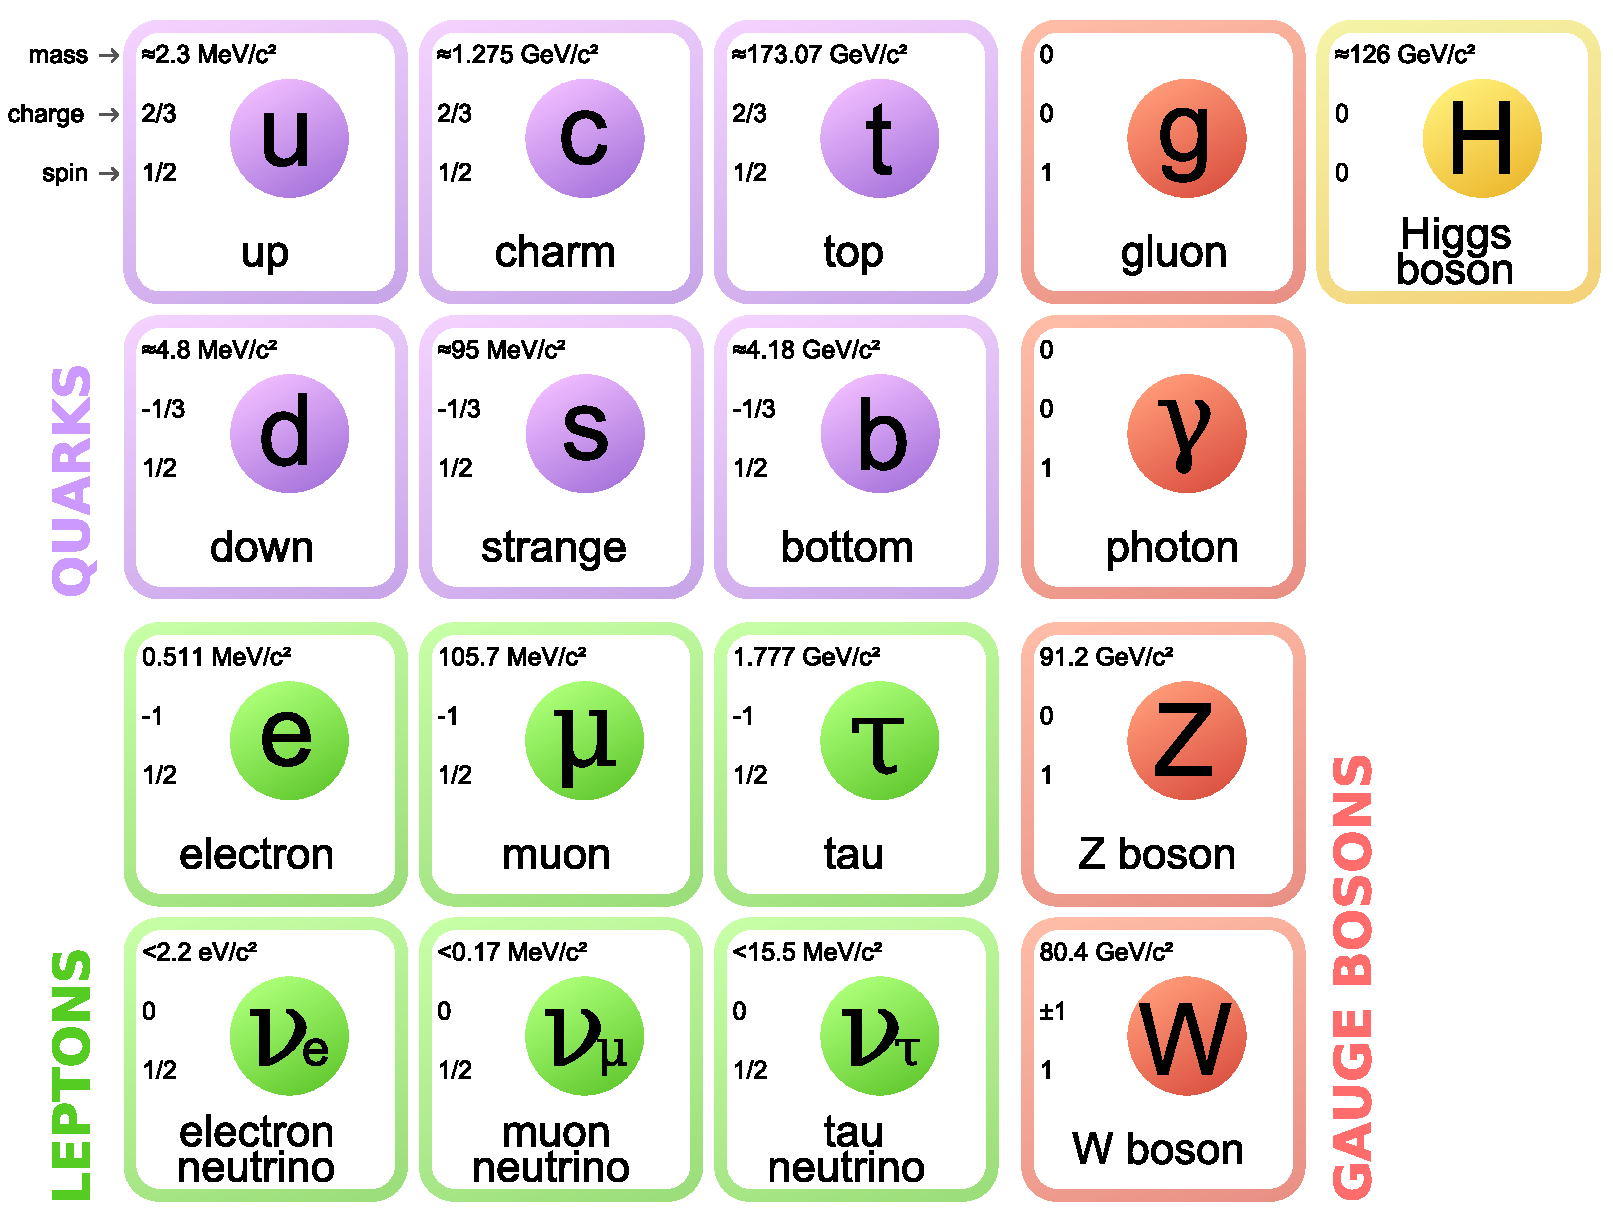
\includegraphics[height=0.33\textwidth]{Standard_Model_of_Elementary_Particles.pdf}
  \caption{Les particules élémentaires du Modèle Standard.}
    \label{fig:sm}
\end{figure}

\subsection{Les fermions}

Les fermions sont des particules élémentaires de spin 1/2, c'est-à-dire qu'elles obéissent la statistique de Fermi-Dirac, et sont ainsi soumises au principe d'exclusion de Pauli. Cela signifie qu'au niveau quantique, deux fermions ne peuvent pas occuper le même état quantique. C'est ce principe qui est responsable de l'existence des couches d'électrons dans les atomes, les électrons étant des fermions.

On dénombre dans le Modèle Standard 12 fermions : 6 quarks et 6 leptons. On groupe les leptons et les quarks 2 par 2 dans des générations :

\begin{description}
  \item[Les fermions] \begin{align*}
    \colvec{2}{e^-}{\nu_e} \colvec{2}{\mu^-}{\nu_\mu} \colvec{2}{\tau^-}{\nu_\tau}
  \end{align*}
  \item[Les quarks] \begin{align*}
    \colvec{2}{u}{d} \colvec{2}{c}{s} \colvec{2}{t}{b}
  \end{align*}
\end{description}

Parmi les leptons, on trouve les électrons, muons et taus, de charge électrique négative. On associe à chaque lepton un partenaire non massif\footnote{On sait maintenant que les neutrinos sont massifs, comme on pourra le voir par la suite}, et électriquement neutre, les neutrinos. Les leptons sont sensibles à l'interaction faible, et les leptons chargés à l'interaction électromagnétique. Les quarks sont des particules massives de charge électrique fractionnaire, et en plus porteur d'une charge de couleur. Ils sont donc sensibles, en plus de l'interaction électromagnétique et l'interaction faible, à l'interaction forte.

A chacune des 12 particules élémentaires est associée une anti-particule, c'est-à-dire une particule de même masse, mais avec des nombres quantiques et une charge opposés : on compte donc 24 constituants élémentaires de la matière.

\subsection{Les interactions fondamentales}

On dénombre trois interactions fondamentales, théorisées et unifiées sous un même formalisme par le Modèle Standard :

\begin{description}
  \item[L'interaction électromagnétique] Cette interaction couple les particules chargés, et a pour médiateur le photon, un boson non massif. C'est l'interaction qui permet la cohésion des atomes.
  \item[L'interaction forte] Cette interaction couple les particules colorées, c'est-à-dire les quarks. Ses médiateurs sont les 8 gluons, bosons non massif. C'est l'interaction qui permet la cohésion du noyau atomique.
  \item[L'interaction faible] Cette interaction couple tous les fermions. Elle a pour médiateurs deux bosons massifs chargés $W^{\pm}$ et un boson neutre massif $Z^0$. Cette interaction est responsable des désintégrations nucléaires $\beta^{\pm}$, qui, au sein du noyau atomique, transforment un proton en neutron ou inversement. C'est la seule interaction à laquelle les neutrinos soient sensibles.
\end{description}

Une quatrième interaction existe, l'interaction gravitationnelle. Cette interaction n'est pas décrite par le Modèle Standard, mais peut être négligée vu la faible masse des particules élémentaires et sa faiblesse face aux trois autres interactions.

\begin{table} \centering
  \begin{tabular}{@{}ccccc@{}} \toprule
    Interaction & boson(s) & masse (\SI{}{\GeV}) & intensité relative & portée (m) \\ \bottomrule
    \multirow{2}{*}{faible} & $W^{\pm}$ & \SI{80.385 \pm 0.015} & \multirow{2}{*}{1} & \multirow{2}{*}{\tilde $10^{-18}$} \\
     & $Z^0$ & \SI{91.1876 \pm 0.0021} & & \\
    forte & $g$ & 0 & 25 & \tilde $10^{-15}$ \\
    électromagnétique & $\gamma$ & 0 & 0.8 & $\infty$ \\
    gravitationnelle & graviton ? & ? & $10^{-41}$ & $\infty$ \\ \bottomrule
  \end{tabular}
  \caption{Les interactions fondamentales et leurs bosons médiateurs.}
  \label{tab:interactions}
\end{table}

\bigskip

Le détails et les bosons médiateurs des interactions fondamentales sont présentés table \ref{tab:interactions}.

\subsubsection{Le boson de Higgs}

Le mécanisme de Higgs permet d'expliquer comment les fermions et les bosons massifs acquièrent leur masse. Théorisé en 1964 par R. Brout, F. Englert et P. Higgs, ce mécanisme prévoit l'existence d'une nouvelle particule de spin 0 (un boson) et massive : le boson de Higgs.

% 
% Le 4 juillet 2012, le CERN a annoncé la découverte d'une nouvelle particule compatible avec le boson de Higgs du Modèle Standard, ayant une masse de \SI{125.9 \pm 0.4}{\GeV}. Cette découverte conforte encore une fois la validité du Modèle Standard.

\section{Paramétrisation théorique}

Avant de rentrer plus en détails dans la paramétrisation théorique du modèle standard, il convient dans un premier temps d'introduire le formalisme mathématique utilisé.

Comme on le verra par la suite, le modèle standard est bâti en exploitant les symétries qui existent entre les différentes particules élémentaires. Le formalisme le plus adapté a cette paramétrisation est le formalisme de Lagrange.

En mécanique classique, les équations d'Euler-Lagrange permettent d'obtenir les équations du mouvement d'une particule :
\begin{align}
  \frac{d}{dt} \left( \frac{\partial L}{\partial \dot{q_i}} \right) - \frac{\partial L}{\partial q_i} &= 0
\end{align}

où $q_i$ sont les coordonnées généralisées des particules, $t$ la variable temps, et $\dot{q_i} = dq_i / dt$. Le Lagrangien L est lui défini par une relation reliant l'énergie cinétique ($T$) et l'énergie potentielle ($V$) :
\begin{align*}
  L &= T - V
\end{align*}

On peut étendre ce formalisme dans le cas au coordonnées continue. Dans ce cas, on transforme les coordonnées discrètes en champ $\phi(x, t)$ (ou $\phi(x)$, et $x$ le quadri-vecteur position). Le Lagrangien devient donc
\begin{align*}
  L(q_i, \dot{q_i}, t) \rightarrow \mathcal{L}\left(\phi, \frac{\partial \phi}{\partial x_\mu}, t\right)
\end{align*}

$\mathcal{L}$ est la densité lagrangienne, et on a la relation
\begin{align*}
  L &= \int \mathcal{L}
\end{align*}

Les équations de Lagrange deviennent
\begin{align} \label{eq:lagrange}
  \frac{\partial}{\partial x_\mu}\left( \frac{\partial \mathcal{L}}{\partial \left( \sfrac{\partial \phi}{\partial x_\mu} \right)} \right) - \frac{\partial \mathcal{L}}{\partial \phi} &= 0
\end{align}

C'est à l'aide de se formalisme que nous allons construire le modèle standard. En effet, une fois le Lagrangien établi, il est possible d'en dériver tout un jeu de règles, que l'on nomme règles de Feynman, et qui permettent de quantifier l'interaction entre les particules élémentaire (vertex d'interaction) et leur propagation (propagateur). Plus de détails seront donnés par la suite, mais il est néanmoins déjà important de noter que, dans le Lagrangien :

\begin{enumerate}
  \item Les propagateurs sont associés aux termes quadratiques du Lagrangien
  \item Les autres termes correspondent aux vertex d'interactions. Les règles de Feynman associées aux vertex sont simplement les termes dans $i\mathcal{L}$ qui contiennent les champs interagissant.
\end{enumerate}

% Afin d'extraire des informations sur les observables physiques, tel que les sections efficaces par exemple, on utilise un développement perturbatif. En effet, la probabilité de transition d'un état initial $\ket{i}$ à un état final $\ket{f}$ est calculée en utilisant la règle d'or de Fermi. Cette règle est obtenue grâce à la théorie des perturbations, en considérant que le temps nécessaire à l'interaction est bien plus petit que le temps nécessaire à l'observation.

% La précision du résultat dépend de l'ordre du calcul. Le premier ordre, celui le plus simple à calculer, correspond à un nombre de vertex de 2, et est appelé calcul à l'arbre (ou \emph{LO}, pour \emph{Leading Order}). Richard Feynman proposa en 1949 un ensemble de règles facilitant le calcul des observables à partir de diagrammes. Lorsque l'on considère des diagrammes d'ordre supérieurs, des boucles font leur apparition, provoquant des divergences lors des calculs. On verra par la suite que ces divergences peuvent être contournées par une redéfinition des couplages de la théorie : c'est la renormalisation.

\subsection{L'interaction électromagnétique (QED)} \label{sec:qed}

On considère le cas d'une particule de masse $m$ à laquelle on associe une fonction d'onde $\Psi(x)$, représenté par un spineur de dimension 4. On définit le Lagrangien $\mathcal{L}$ par
\begin{align} \label{eq:lagrangien_qed_simple}
  \mathcal{L} &= i \bar{\Psi} \gmu \dmuc \Psi -m \bar{\Psi}\Psi
\end{align}
où $\gmu$ sont des matrices $4 \times 4$, appelées matrices de Dirac. Ce choix, complètement arbitraire, permet de retrouver l'équation de Dirac\footnote{$\left(i \gmuc \dmu - m\right) \Psi = 0$} lorsque l'on applique \eqref{eq:lagrange}. Intéressons nous maintenant plus particulièrement aux symétries de ce Lagrangien. On s'aperçoit rapidement qu'il est invariant par changement de phase (aussi appelé jauge). En effet, en effectuant la transformation
\begin{align*}
  \Psi &\rightarrow \Psi^\prime = e^{i\theta}\Psi
\end{align*}
et en notant que
\begin{align*}
  \dmu \Psi &\rightarrow e^{i\theta}\dmu \Psi\\
  \bar{\Psi} = \Psi^\dagger \gzeroc &\rightarrow e^{-i\theta}\bar{\Psi}
\end{align*}

On a bien
\begin{align*}
  \mathcal{L} &\rightarrow \mathcal{L}^\prime = \mathcal{L}
\end{align*}

On dit que le Lagrangien est invariant de jauge globale (la phase est la même dans tout l'espace-temps). Les transformations du genre $U(\theta) = e^{i\theta}, \theta \in \mathbb{C}$ forment le groupe de symétrie unitaire Abélien $U(1)$.

Cette invariance a une conséquence très importante. En effet, d'après le théorème de N{\oe}ther, toute symétrie interne ou externe correspond à une quantité conservée. L'exemple le plus connu est probablement la conservation de l'énergie d'un système, cause directe de l'invariance par translation dans le temps. Dans le cas de notre Lagrangien, cette invariance conduit à l'équation de conservation
\begin{align} \label{eq:e_current}
  \dmu j^\mu &= 0 & \text{avec} && j^\mu &= -e \bar{\Psi} \gmuc \Psi
\end{align}
Le courant électronique $j^\mu$ est donc conservé, et on en déduit que la charge, définie par $Q = \int j^0 d^3x$ est aussi conservée.

Cette symétrie globale de jauge n'est pas la plus générale. Il serait en effet plus satisfaisant si la phase pouvait varier localement ($\theta \rightarrow \theta(x)$). Malheureusement, le Lagrangien \eqref{eq:lagrangien_qed_simple} n'est pas invariant lorsque l'on effectue la transformation\footnote{On a introduit l'opérateur de charge $Q$, dont les valeurs propres sont $\pm 1$ pour les leptons, et $\pm\frac{1}{3}$ et $\pm\frac{2}{3}$ pour les quarks. $Q$ est le générateur du groupe $U(1)$.}
\begin{align*}
  \Psi \rightarrow e^{i\theta(x)Q}\Psi
\end{align*}

En effet, la dérivée de $\Psi$ se transforme maintenant comme
\begin{align} \label{eq:brisure_jauge_local}
  \dmu \Psi \rightarrow e^{i\theta(x)}\dmu\Psi + iQe^{i\theta(x)}\Psi\dmu\theta(x)
\end{align}

Le terme $\dmu\theta(x)$ brise l'invariance de jauge. Il est cependant intéressant de voir ce qu'il se passe si on impose l'invariance du Lagrangien.

Pour ce faire, il suffit de remplacer la dérivée $\dmu$ dans la définition du Lagrangien par une autre dérivée $D_\mu$, appelée dérivée covariante. Cette nouvelle dérivée se transforme comme
\begin{align*}
  D_\mu\Psi &\rightarrow e^{i\theta(x)Q}D_\mu\Psi
\end{align*}
Afin de pouvoir écrire une telle dérivée, il est nécessaire d'introduire un nouveau champ vectoriel, $A_\mu$, qui se transforme de façon à annuler le terme en $\dmu \theta(x)$ dans \eqref{eq:brisure_jauge_local}. On définit la dérivée covariante par\footnote{le terme $e$ (charge électrique) est purement conventionnel}
\begin{align*}
  D_\mu &= \dmu + ieQA_\mu
\end{align*}
où $A_\mu$ se transforme comme
\begin{align} \label{eq:photon_jauge_transformation}
  A_\mu &\rightarrow A_\mu - \frac{1}{e}\dmu\theta(x)
\end{align}

En remplaçant $\dmu$ par $D_\mu$, on obtient le Lagrangien invariant locale de jauge
\begin{align*}
  \mathcal{L} &= \Psib\left(i\gmuc\dmu - m\right)\Psi - e\Psib \gmuc Q A_\mu \Psi
\end{align*}

En forçant le Lagrangien à être invariant locale de jauge, nous sommes obligé d'introduire un nouveau champ vectoriel (champ de jauge): c'est le photon. Afin de vraiment interpréter ce nouveau champ comme le photon, il est nécessaire d'ajouter dans le Lagrangien un terme correspondant à l'énergie cinétique du photon. Le seul candidat invariant lors de la transformation \eqref{eq:photon_jauge_transformation} doit être construit à partir du tenseur
\begin{align*}
  F_{\mu\nu} &= \dmu A_\nu - \partial_\nu A_\mu
\end{align*}

On obtient donc finalement le Lagrangien décrivant l'interaction électromagnétique
\begin{align} \label{eq:l_qed}
  \mathcal{L}_{\text{QED}} &= \Psib\left(i\gmuc\dmu - m\right)\Psi - e\Psib \gmuc Q A_\mu \Psi - \frac{1}{4} F_{\mu\nu}F^{\mu\nu}
\end{align}
Un dernier point reste à remarquer. Il n'est pas possible d'ajouter un terme $\frac{1}{2}m^2A_\mu A^\mu$ sans violer l'invariance locale de jauge. Le photon doit donc être sans masse.

\bigskip

Imposer l'invariance locale de jauge du Lagrangien nous a forcé à introduire une nouvelle particule, sans masse : le photon. Nous verrons par la suite qu'imposer l'invariance locale de jauge nous permet de décrire aussi bien l'interaction faible (via l'unification électrofaible) que l'interaction forte.

\subsection{L'interaction forte (QCD)} \label{sec:qcd}

Le modèle des quarks est une grande réussite, et a permis d'expliquer de façon élégante la prolifération de nouvelles particules ($\pi^{0/+/-}$, $K$, $\eta$, \ldots). Cependant, la découverte du $\Delta^{++}$ en 1951 remet en cause le modèle. En effet, cet hadron est composé de trois quarks $u$. Le principe d'exclusion de Pauli interdit deux particules de spin $\frac{1}{2}$ d'être dans le même état quantique. Étant de spin $\frac{3}{2}$, $\Delta^{++}$ est forcément composée de deux $u$ de même spin, ce qui n'est pas autorisé par le principe d'exclusion.

La solution à ce problème est d'introduire un nouveau nombre quantique, similaire à la charge électrique : la charge de couleur. Un quark peut donc exister en trois couleurs différentes : rouge ($R$), vert ($V$), bleu ($B$), et un anti-quark en cyan ($\bar{R}$), magenta ($\bar{V}$) et jaune ($\bar{B}$)\footnote{Par analogie à la synthèse des couleurs}. En réalité, $\Delta^{++}$ est composé de $u_R u_V u_B$, ce qui permet de s'affranchir du principe d'exclusion de Pauli : chaque quark est dans un état quantique différent. Afin de restreindre l'effet de l'introduction de ce nombre quantique, les états liés doivent être neutres du point de vue de la couleur. Cela implique donc qu'il ne peut exister que des états liés $q_i\bar{q}_i$, $q_R q_V q_B$ ou $\bar{q}_{\bar{R}} \bar{q}_{\bar{V}} \bar{q}_{\bar{B}}$. où $i$ est la couleur ($R$, $V$ ou $B$)\footnote{On peut aussi imaginer des états liés à 4 ou 5 quarks non colorés. Ils n'ont encore jamais été observé, mais de nombreuses recherches sont actuellement en cours}.

% Ce nouveau nombre quantique permet aussi d'expliquer pourquoi il n'existe pas d'état lié $qq$ ou $\bar{q}\bar{q}$ : un état lié de quarks doit apparaître "blanc", c'est-à-dire non coloré. Ainsi, un méson est toujours un état lié $q_i\bar{q}_i$, où $i$ est la couleur ($R$, $V$ ou $B$), et un hadron un état $q_R q_V q_B$ ou $\bar{q}_{\bar{R}} \bar{q}_{\bar{V}} \bar{q}_{\bar{B}}$.

\bigskip

Le Lagrangien de la QCD est basé sur la même idée que section \ref{sec:qed}, à la seule différence que l'on remplace la symétrie de jauge $U(1)$ par $SU(3)$, puisque chaque quark existe en trois couleurs différentes. Le Lagrangien devient donc
\begin{align*}
  \mathcal{L} &= \bar{q}_i^j\left(i\dmu\gmuc -m\right)q_i^j
\end{align*}
où $i$ représente la charge de couleur et $j$ la saveur du quark.

Comme précédemment, on requiert que le Lagrangien soit invariant sous une transformation de jauge locale, c'est-à-dire qu'il soit invariant lorsque l'on applique la transformation
\begin{align} \label{eq:su3_jauge}
  q(x) \rightarrow Uq(x) = e^{i \theta_a(x) T_a}q(x) \simeq \left(1 + i\theta_a(x) T_a\right)q(x)
\end{align}
où $T_a$ sont un ensemble de 8 matrices, et $\theta_a$ sont les paramètres du groupe. Un choix conventionnel pour $T_a$ est $\frac{\lambda_a}{2}$, où $\lambda$ sont les matrices de Gell-Mann. Ce groupe est non Abélien puisque les générateurs du groupe $T_a$ ne commutent pas entre eux :
\begin{align*}
  \left[T_i, T_j\right] &= i f_{ijk} T_k
\end{align*}

Les coefficients $f_{ijk}$ sont réels et sont appelées constantes de structure du groupe. Après la transformation \eqref{eq:su3_jauge}, on a
\begin{align*}
  \dmu q \rightarrow (1 + i\theta_a(x) T_a)q + iT_aq\dmu\theta_a(x)
\end{align*}

L'invariance de jauge est donc ici aussi violée par le terme en $\dmu\theta_a$. On procède de la même façon que pour la QED. On introduit la dérivée covariante
\begin{align*}
  D_\mu &= \dmu + igT_aG_\mu^a
\end{align*}

Cette fois, nous sommes obligés d'introduire non pas un champ vectoriel, mais huit, un pour chaque générateur du groupe de symétrie. Ces nouveaux champs se transforment de la façon suivante :
\begin{align*}
  G_\mu^a \rightarrow G_\mu^a - \frac{1}{g} \dmu \theta_a - f_{abc}\theta_bG_\mu^c
\end{align*}

Le dernier terme est nécessaire puisque $SU(3)$ est un groupe non Abélien. Pour finir, il suffit d'ajouter les termes d'énergie cinétique pour chacun des huit nouveaux champs au Lagrangien pour obtenir la paramétrisation de la QCD :
\begin{align} \label{eq:l_qcd}
  \mathcal{L}_{\text{QCD}} &= \bar{q}_i^j\left(i\dmu\gmuc -m\right)q_i^j - g\left(\bar{q}_i^j\gmuc T_a q_i^j\right)G_\mu^a - \frac{1}{4}G_{\mu\nu}^aG_a^{\mu\nu}
\end{align}

\begin{figure}[t!] \centering
  \subcaptionbox{\label{fig:3_gluons_vertex}}[.4\linewidth]{
  \begin{fmfgraph*}(180,100)
    \fmfpen{0.5}
    \fmfleft{i1}
    \fmfright{o1,o2}
    \fmf{gluon}{i1,v1,o1}
    \fmf{gluon}{v1,o2}
    \fmfdot{v1}
  \end{fmfgraph*}}\qquad%
  \subcaptionbox{\label{fig:4_gluons_vertex}}[.4\linewidth]{
  \begin{fmfgraph*}(180,100)
    \fmfpen{0.5}
    \fmfleft{i1,i2}
    \fmfright{o1,o2}
    \fmf{gluon}{i1,v1,o1}
    \fmf{gluon}{i2,v1,o2}
    \fmfdot{v1}
  \end{fmfgraph*}}
  \caption{Vertex d'interaction à 3 (\protect\subref{fig:3_gluons_vertex}) et 4 (\protect\subref{fig:4_gluons_vertex}) gluons.}
  \label{fig:gluon_self_interaction}
\end{figure}

Le tenseur $G_{\mu\nu}$ est défini de façon analogue à $F_{\mu\nu}$, mais, étant donné le caractère non Abélien du groupe, des termes supplémentaires sont présent :
\begin{align*}
  G_{\mu\nu}^a &= \dmu G_\nu^a - \partial_\nu G_\mu^a - g f^{abc} G_{b,\mu} G_{c,\nu}
\end{align*}

On peut finalement interpréter les huit nouveaux champs vectoriels comme les huit gluons du Modèle Standard. Le Lagrangien \eqref{eq:l_qcd} représente donc l'interaction entre des quarks colorés et des bosons vecteur $G_\mu$, les gluons, avec une constante de couplage $g$. Comme pour le photon, il n'est pas possible d'introduire un terme de masse sans briser l'invariance locale de jauge. Les gluons doivent donc être sans masse.

Une des propriétés remarquables du tenseur $G_{\mu\nu}^a$ est que, contrairement à $F_{\mu\nu}$, il contient des termes d'auto-interaction ($\propto G_\mu^b G_\nu^c$). En effet, les gluons étant médiateur de l'interaction force et portant eux même une charge de couleur, ils peuvent interagir entre eux, comme on peut le voir figure \ref{fig:gluon_self_interaction}.

\subsection{L'unification électrofaible}

On a pu voir précédemment que les médiateurs de l'interaction faible sont les bosons chargés $W^{\pm}$, ainsi que le boson neutre $Z^0$. On peut voir figure \ref{fig:w_decay} la désintégration d'un boson $W$ en $e\nu$.

\begin{figure} \centering
  \subcaptionbox{$W^- \rightarrow e^- \bar{\nu}_e$}[.4\linewidth]{
  \begin{fmfgraph*}(180,100)
    \fmfpen{0.5}
    \fmfleft{i1}
    \fmfright{o1,o2}
    \fmf{boson,label=$W^-$}{i1,v1}
    \fmf{fermion}{o1,v1,o2}
    \fmfdot{v1}
    \fmflabel{$e^-$}{o2}
    \fmflabel{$\bar{\nu}_e$}{o1}
  \end{fmfgraph*}}\qquad%
  \subcaptionbox{$W^+ \rightarrow e^+ \nu_e$}[.4\linewidth]{
  \begin{fmfgraph*}(180,100)
    \fmfpen{0.5}
    \fmfleft{i1}
    \fmfright{o1,o2}
    \fmf{boson,label=$W^+$}{i1,v1}
    \fmf{fermion}{o1,v1,o2}
    \fmfdot{v1}
    \fmflabel{$e^+$}{o1}
    \fmflabel{$\nu_e$}{o2}
  \end{fmfgraph*}}
  \caption{Désintégration des bosons $W^{\pm}$ en $e\nu$}
  \label{fig:w_decay}
\end{figure}

De façon analogique au courant électromagnétique \eqref{eq:e_current}, on introduit le courant faible chargé

\begin{align*}
  j^\mu_{\text{w}} &= G \bar{u}_\nu \gmuc u_e
\end{align*}
où $G$ est la constante de couplage, et $u_i$ un spineur de Dirac associée à la particule $i$.

Ce courant est invariant lors des transformations de parité. Malheureusement, bien que permettant d'expliquer la plupart des observations sur la désintégration $\beta$, cette formulation du courant échoue sur d'autres points. En effet, en étudiant la désintégration $\beta$ de nombreux atomes (tel que le cobalt \citep{co60}), il s'est avéré que l'interaction faible ne fait apparaître que des neutrino d'hélicité gauche ($\nu_L$) ou des anti-neutrino d'hélicité droite ($\bar{\nu}_R$) : ceci est une violation directe de l'invariance de la parité, et il est nécessaire que le courant faible reflète ceci.

Parmi les invariants de Lorentz qui ne sont pas invariants par parité, on trouve les structures $\frac{1}{2}\gmuc(1 - \gfivec)$ et $\frac{1}{2}\gmuc(1 + \gfivec)$. Si l'on omet le terme $\gmuc$, nécessaire pour obtenir le courant, ces deux structures sont respectivement les projecteurs de chiralité gauche et droite. Lorsque la masse devient négligeable devant l'énergie, la chiralité se confond avec l'hélicité. Le neutrino n'ayant pas de masse, le projecteur de chiralité projette aussi l'hélicité. L'expérience nous oblige donc à choisir la structure $\frac{1}{2}\gmuc(1 - \gfivec)$ (structure $V - A$, pour Vecteur - Axial), puisque l'interaction faible ne couple uniquement que les neutrino d'hélicité gauche. Le courant faible chargé devient alors

\begin{align}
  j^\mu_{\text{w}} &= G \bar{u}_\nu \frac{1}{2} \gmuc \left(1 - \gfivec \right) u_e
\end{align}

On peut ré-exprimer le courant faible en décomposant $u$ en $u_L$ et $u_R$. En omettant la constante de couplage $G$, et en considérant uniquement le cas de l'électron $e$, on obtient alors
\begin{align*}
&\left. \begin{aligned}
  J_\mu^+ &= \bar{u}_\nu \frac{1}{2} \gmu \left(1 - \gfivec \right) u_e \\
   &\equiv \bar{\nu} \frac{1}{2} \gmu \left(1 - \gfivec \right) e = \bar{\nu}_L \gmu e_L
\end{aligned} \right\}\,W^+ \rightarrow e^+ \nu_e\\
&\left. \begin{aligned}
  J_\mu^- &= \bar{u}_e \frac{1}{2} \gmu \left(1 - \gfivec \right) u_\nu \\
   &\equiv \bar{e} \frac{1}{2} \gmu \left(1 - \gfivec \right) \nu = \bar{e}_L \gmu \nu_L
\end{aligned} \right\}\,W^- \rightarrow e^- \bar{\nu}_e
\end{align*}
où $J_\mu^+$ et $J_\mu^-$ sont respectivement les courants liés aux $W^+$ et $W^-$.

On peut réécrire de façon plus succincte l'équation précédente en introduisant un nouveau doublet, $\chi_L$, défini comme
\begin{align*}
  \chi_L = \colvec{2}{\nu}{e^-}_L
\end{align*}
ainsi que les opérateur $\tau_+$ et $\tau_-$, défini comme $\tau_{\pm} = \frac{1}{2}\left( \tau_1 \pm i\tau_2 \right)$ ($\tau_i$ sont les trois matrices de Pauli). Les courants faibles chargés peuvent être réécrit comme
\begin{align*}
  J_\mu^+ &= \bar{\chi}_L \gmu \tau_+ \chi_L \\
  J_\mu^- &= \bar{\chi}_L \gmu \tau_- \chi_L
\end{align*}

La structure $V-A$ de l'interaction faible disparaît pour laisser apparaître une interaction purement vectorielle entre fermions d'hélicité gauche, interaction ressemblant fortement à celle de QED. Cette observation nous laisse entrevoir une possible unification entre l'interaction faible et électromagnétique : l'interaction électrofaible.

\bigskip

On a défini $J_\mu^{\pm}$ à l'aide des matrices de Pauli, générateurs du groupe de symétrie $SU(2)$. Essayons de définir le courant neutre $J_\mu^3$ :
\begin{align*}
  J_\mu^3 &= \bar{\chi}_L \gmu \frac{1}{2} \tau_3 \chi_L = \rowvec{2}{\bar{\nu}}{e^+}_L \gmu \frac{1}{2} \begin{pmatrix}
    1 & 0 \\
    0 & -1
  \end{pmatrix} \colvec{2}{\nu}{e^-}_L \\
  &= \frac{1}{2} \bar{\nu}_L \gmu \nu_L - \frac{1}{2} e^+_L \gmu e^-_L
\end{align*}

On peut ainsi former avec $J_\mu^i$, $i = 1 \ldots 3$ un triplet "d'isopin" de courant faible
\begin{align*}
  J_\mu^i &= \bar{\chi}_L \gmu \frac{1}{2} \tau_i \chi_L
\end{align*}

On définit l'équivalent de la charge par $T^i = \int J_0^i d^3x$. Ces charges forment les générateurs du groupe $SU(2)_L$, avec comme relation de commutation
\begin{align*}
  \left[ T^i, T^j \right] &= i \epsilon_{ijk}T^k
\end{align*}

On peut être tenter d'interpréter $J_\mu^3$ comme le courant faible neutre associé au $Z^0$. Malheureusement, ceci est incorrect, puisque le courant que l'on vient d'écrire ne couple que des particules de chiralité gauche, contrairement au $Z^0$, qui couple à la fois les chiralités gauche et droite. Cependant, le courant électromagnétique est aussi un courant neutre, qui couple les deux chiralités. On rappelle que $ej^{EM}_\mu = e\Psib \gmu Q \Psi$, où $Q$ est l'opérateur de charge.

Afin de sauver la symétrie $SU(2)_L$, nous sommes contraint de faire intervenir l'interaction électromagnétique afin d'avoir un courant neutre faible convenable. Nous étendons la symétrie en formant deux combinaisons orthogonales qui ont des transformations défini sous $SU(2)_L$ : la première combinaison, $J_\mu^3$ permet de former le triplet d'isospin. La seconde combinaison $j_\mu^Y$ doit rester invariant sous $SU(2)_L$ : c'est le courant neutre d'hypercharge (on généralise ici la charge électrique), donné par
\begin{align*}
  j_\mu^Y &= \Psib \gmu Y \Psi
\end{align*}
et on définit l'hypercharge $Y$ par une relation reliant la charge électrique $Q$ et la "charge" neutre faible $T^3$ :
\begin{align} \label{eq:q_t_y}
  Q &= T^3 + \frac{Y}{2}
\end{align}

$Y$ est ainsi un générateur du groupe $U(1)_Y$, et $\vec{T}$ les générateurs du groupe $SU(2)_L$. On étend ainsi le groupe $SU(2)_L$ au groupe de symétrie $SU(2)_L \times U(1)_Y$ en unifiant les interactions faible et électromagnétique \citep{PhysRevD.2.1285,PhysRevLett.19.1264}.

On a alors les doublets d'isopin $\chi_L$, composés des fermions de même famille de chiralité gauche et qui se transforment sous $SU(2)_L$ et $U(1)_Y$. Enfin, on classifie les fermions de chiralité droite dans des singlets d'isospin, invariant sous $SU(2)_L$ et qui se transforment sous $U(1)_Y$.
\begin{align*}
  \chi_L &= \colvec{2}{\nu}{e}_L, \colvec{2}{u}{d}_L & & \text{doublet d'isospin} \\
  \Psi_R &= e_R, u_R \text{ ou } d_R & & \text{singlet d'isospin}
\end{align*}

\bigskip

On procède maintenant de la même façon que pour QED et QCD. On introduit le Lagrangien $L$ défini par
\begin{align*}
  \mathcal{L} &= \bar{\chi}_L\left(i\gmuc\dmu - m\right)\chi_L + \Psib_R \left(i\gmuc\dmu - m\right) \Psi_R
\end{align*}
$\chi_L$ et $\Psi_R$ se transforment respectivement sous $SU(2)_L \times U(1)_Y$ et $U(1)_Y$, selon les relations
\begin{align*}
  \chi_L &\rightarrow \chi^\prime_L = e^{i\vec{\theta}(x) \cdot \vec{T}\,+\,i\iota(x) Y}\chi_L \\
  \Psi_R &\rightarrow \Psi_R^\prime = e^{i\iota(x) Y}\Psi_R
\end{align*}

On impose maintenant l'invariance locale de jauge au Lagrangien. On remplace la dérivée par deux dérivées covariantes $D_\mu^i$, définies par
\begin{align*}
  D_\mu^1 &= \dmu + ig_1\frac{1}{2}\vec{\tau} \cdot \vec{W}_\mu + ig_2 \frac{Y}{2} B_\mu\text{, avec }\frac{1}{2} \vec{\tau} = \vec{T}\\
  D_\mu^2 &= \dmu + ig_2 \frac{Y}{2} B_\mu
\end{align*}

Encore une fois, imposer l'invariance locale de jauge nous force à introduire quatre nouveaux champs vectoriels, un pour chaque générateur du groupe de symétrie : un triplet d'isospin $\vec{W}_\mu$ et un singlet $B_\mu$. Ces nouveaux champs se transforment comme
\begin{align*}
  B_\mu &\rightarrow B_\mu - \frac{1}{g_2} \dmu \iota(x) \\
  W^i_\mu &\rightarrow W^i_\mu - \frac{1}{g_1} \dmu \theta^i(x) - \epsilon^{ijk} \theta_j(x) W_{k,\mu}
\end{align*}

Afin de compléter le Lagrangien, il nous reste à ajouter les termes cinétiques des quatre nouveaux champs. On introduit donc quatre tenseurs, défini par
\begin{align*}
  B_{\mu\nu} &= \dmu B_\nu - \partial_\nu B_\mu\\
  W^i_{\mu\nu} &= \dmu W^i_\nu - \partial_\nu W^i_\mu - g_1 \epsilon^{ijk} W_{j,\mu} W_{k,\nu}
\end{align*}

En ajoutant tous les termes ensemble, on obtient le Lagrangien de l'interaction électrofaible :
\begin{align} \label{eq:l_ewk}
 \begin{aligned}
   \mathcal{L}_{\text{EWK}} =\ &\bar{\chi}_L \gmuc \left( i\dmu - g_1 \frac{1}{2} \vec{\tau} \cdot \vec{W}_\mu - g_2 \frac{Y}{2} B_\mu \right) \chi_L + \Psib_R \gmuc \left( i\dmu - g_2 \frac{Y}{2} B_\mu \right) \Psi_R \\
 &- \frac{1}{4}B_{\mu\nu}B^{\mu\nu} - \frac{1}{4}\vec{W}_{\mu\nu} \cdot \vec{W}^{\mu\nu}
 \end{aligned}
\end{align}

\begin{table} \centering
  \begin{tabular}{@{}cccccccc@{}} \toprule
    \multicolumn{3}{c}{Génération} & \multicolumn{5}{c}{Nombres quantiques} \\
    I & II & III & $SU(3)_c$ & $SU(2)_L$ & Y & $T^3$ & Q \\ \midrule
    \multirow{2}{*}{$\colvec{2}{\nu_e}{e^-}_L$} & \multirow{2}{*}{$\colvec{2}{\nu_\mu}{\mu^-}_L$} & \multirow{2}{*}{$\colvec{2}{\nu_\tau}{\tau^-}_L$} & \multirow{2}{*}{1} & \multirow{2}{*}{2} & \multirow{2}{*}{-1} & 1/2 & 0 \\
    & & & & & & -1/2 & -1\\
    $e_R^-$ & $\mu_R^-$ & $\tau_R^-$ & 1 & 1 & -2 & 0 & -1 \\ \midrule
    \multirow{2}{*}{$\colvec{2}{u}{d}_L$} & \multirow{2}{*}{$\colvec{2}{c}{s}_L$} & \multirow{2}{*}{$\colvec{2}{t}{b}_L$} & \multirow{2}{*}{3} & \multirow{2}{*}{2} & \multirow{2}{*}{$\sfrac{1}{3}$} & 1/2 & $\sfrac{+2}{3}$ \\
    & & & & & & -1/2 & $\sfrac{-1}{3}$\\
    $u_R$ & $c_R$ & $t_R$ & 3 & 1 & $\sfrac{4}{3}$ & 0 & $\sfrac{+2}{3}$ \\
    $d_R$ & $s_R$ & $d_R$ & 3 & 1 & $\sfrac{-2}{3}$ & 0 & $\sfrac{-1}{3}$ \\ \midrule
    \multirow{2}{*}{$\colvec{2}{\phi^+}{\phi^0}$} & & & \multirow{2}{*}{1} & \multirow{2}{*}{2} & \multirow{2}{*}{1} & 1/2 & 1 \\
    & & & & & & -1/2 & 0 \\ \bottomrule
  \end{tabular}
  \caption{Les nombres quantiques des particules élémentaires. Le doublet de Higgs a été ajouté sur la dernière ligne afin d'avoir un aperçu de ses nombres quantiques.}
  \label{tab:nbr_quantiques}
\end{table}

Les termes en $m\bar{\chi}_L\chi_L$ et $m\Psib\Psi$ ont disparu du Lagrangien final. En effet, ces termes ne sont pas invariant sous transformation locale de jauge : les fermions perdent donc leur masse lors de l'unification électrofaible. De même, comme pour le photon ou les gluons, il n'est pas possible d'ajouter des termes de masse pour les nouveaux bosons introduit : ils doivent donc être sans masse.

\bigskip

Cette formulation de l'interaction faible permet de retrouver les deux bosons chargés de l'interaction faible, $W^{\pm}$, défini par
\begin{align*}
  W^{\pm} &= \frac{1}{\sqrt{2}} \left(W^1 \mp iW^2 \right)
\end{align*}

Il n'est cependant pas possible d'interpréter $W^3$ comme le boson $Z^0$, ni $B$ comme le photon, pour les mêmes raisons que précédemment. Tout n'est pas perdu, et nous verrons par la suite que ces deux champs vectoriels se mélangent pour former le $Z^0$ et le photon.

\bigskip

Comme formulée aux travers de ce manuscrit, la théorie électrofaible a trois problèmes
\begin{enumerate}
  \item L'interaction électrofaible ne couple que les fermions d'une même famille. Si cela ne pose aucun soucis théorique, l'expérience montre que l'interaction faible couple des familles différentes\footnote{Par exemple, on observe $K^+ \rightarrow \pi^+ \pi^0$ où un quark $s$ se transforme en quark $d$}. Cabibbo apportât la solution en 1963 : il postula que les états propre de masse des quarks n'étaient pas états propres de l'interaction faible. Autrement dit, les quarks que nous observons sont en réalité un mélange entre les quarks états propre de l'interaction faible. Si on désigne avec un $^\prime$ les états propres de l'interaction faible, l'idée de Cabibbo s'écrit
  \begin{align*}
    \colvec{2}{d^\prime}{s^\prime} &= \begin{pmatrix}
      \cos{\theta_c} & \sin{\theta_c} \\
      - \sin{\theta_c} & \cos{\theta_c}
    \end{pmatrix} \colvec{2}{d}{s}
  \end{align*}
  où $\theta_c$ est l'angle de Cabibbo, et représente le mélange entre les différentes saveur de quarks. En réalité, le passage de l'espace vectoriel formé par les états propres de l'interaction faible à l'espace vectoriel formé par les états propres de masse s'effectue par une rotation d'angle $\theta_c$. La valeur de $\theta_c$ est déterminée de façon très précise par l'expérience à \SI{13.015}{\degree}.
  
  Le mécanisme a été ensuite généralisé par Kobayashi et Maskawa aux trois générations de quarks \citep{CKM}. La matrice de rotation de Cabibbo devient une matrice $3 \times 3$ : la matrice CKM.
  \begin{align*}
    \colvec{3}{d^\prime}{s^\prime}{b^\prime} &= \begin{pmatrix} V_{ud} & V_{us} & V_{ub} \\ V_{cd} & V_{cs} & V_{cb} \\ V_{td} & V_{ts} & V_{tb} \end{pmatrix} \colvec{3}{d}{s}{b}
  \end{align*}
  
  Expérimentalement \citep{pdg}, ses valeurs sont :
  \begin{align*}
    V_{\text{CKM}} &= \begin{pmatrix}
      0.97427 \pm 0.00015 & 0.22534 \pm 0.00065 & 0.00351^{+0.00015}_{-0.00014} \\
      0.22520 \pm 0.00065 & 0.97344 \pm 0.00016 & 0.0412^{+0.0011}_{-0.0005} \\
      0.00867^{+0.00029}_{-0.00031} & 0.0404^{+0.0011}_{-0.0005} & 0.999146^{+0.000021}_{-0.000046}      
    \end{pmatrix}
  \end{align*}

  \item On a vu qu'imposer l'invariance locale de jauge fait apparaître quatre nouveaux champs, forcément sans masse. Néanmoins, les bosons $W$ et $Z$ sont massifs. Afin de pouvoir continuer à interpréter ces nouveaux champs comme les médiateurs de l'interaction faible, il est nécessaire d'introduire un mécanisme qui permet de donner une masse à ces médiateurs : c'est le mécanisme de Higgs, qui, au travers de l'introduction d'un nouveau champ scalaire et d'une brisure de la symétrie électrofaible, permet de d'ajouter un terme de masse au Lagrangien sans briser l'invariance locale de jauge.
  
  \item Les termes de masses des fermions ne sont pas invariant sous une transformation de jauge locale : ils doivent être enlevés du Lagrangien. On verra par la suite que le même mécanisme permet d'ajouter des termes de masses au Lagrangien invariant de jauge locale.
  
\end{enumerate}

\subsection{Brisure spontanée de symétrie}

Intéressons nous au Lagrangien d'un champ scalaire complexe $\phi = \frac{1}{\sqrt{2}} (\phi_1 + i \phi_2)$ :
\begin{align*}
  \mathcal{L} &= (\dmu \phi )^\star ( \dmuc \phi ) - V(\phi) = \frac{1}{2} \left( \dmu \phi_1 \right)^2 + \frac{1}{2} \left( \dmu \phi_2 \right)^2 - V(\phi) \\
  V(\phi) &= \mu^2 \phi^\star \phi + \lambda \left( \phi^\star \phi \right)^2 = \frac{1}{2} \mu^2 \left( \phi_1^2 + \phi_2^2 \right) + \frac{1}{4} \lambda \left( \phi_1^2 + \phi_2^2 \right)^2,\ \lambda > 0
\end{align*}
% $\mu^2 > 0$, ce Lagrangien décrit deux champ scalaires de masse $\mu$.

Le minimum du potentiel est
\begin{align*}
  \frac{\partial V}{\partial \phi } &= 0 &\rightarrow&& \left( \phi_1^2 + \phi_2^2 \right) = v^2 = - \frac{\mu^2}{\lambda}
\end{align*}

Si on considère $\mu^2 < 0$, c'est l'équation d'un cercle de rayon $v$. Le potentiel admet ainsi une infinité de minimum, différents de $\phi = 0$ : la symétrie du Lagrangien est brisée\footnote{$V(\phi)$ est le potentiel le plus simple qui permet d'exhiber la brisure de la symétrie}. Cependant, les calculs perturbatifs, qui sont au c{\oe}ur de la théorie qui permet de construire le Modèle Standard, doivent être réalisés autour du minimum du potentiel. On réexprime donc le champ scalaire par une expansion autour de son minimum. Par convention, on choisi $\phi_2 = 0$ et donc $\phi_1 = \phi = v$ au minimum. On a alors
\begin{align*}
  \phi(x) = \frac{1}{\sqrt{2}} \left[ v + \eta(x) + i\xi(x) \right]
\end{align*}
où $\eta(x)$ est une variation infinitésimale le long du rayon du cercle, et $\xi(x)$ une variation infinitésimale perpendiculaire à $\eta(x)$.

On réinjecte la nouvelle paramétrisation dans le Lagrangien. On trouve
\begin{align*}
  \mathcal{L} &= \frac{1}{2}\left( \dmu \xi \right)^2 + \frac{1}{2}\left( \dmu \eta \right)^2 + \mu^2\eta^2 + \ldots
\end{align*}
où on a omis les termes croisés entre $\eta$ et $\xi$. $\mu^2$ étant négatif, on peut interpréter le troisième terme comme le terme de masse du champ $\eta$, avec $m_\eta = \sqrt{-2\mu^2}$. Cependant, aucun terme de masse n'apparaît pour le champ $\xi$ : la brisure de symétrie permet donc d'introduire un champ massif, accompagné d'un autre champ, sans masse, que l'on nomme boson de Goldstone.

Il existe cependant un moyen de faire disparaître ce champ non massif. En remplaçant le champ complexe par un doublet de $SU(2)_L$, et en imposant le Lagrangien a être invariant locale de jauge, les bosons de Goldstone vont se mélanger pour donner naissance à un champ scalaire massif : c'est le mécanisme de Higgs, introduit historiquement par \citet{PhysRevLett.13.321,PhysRevLett.13.508,PhysRevLett.13.585}.

\begin{figure} \centering
  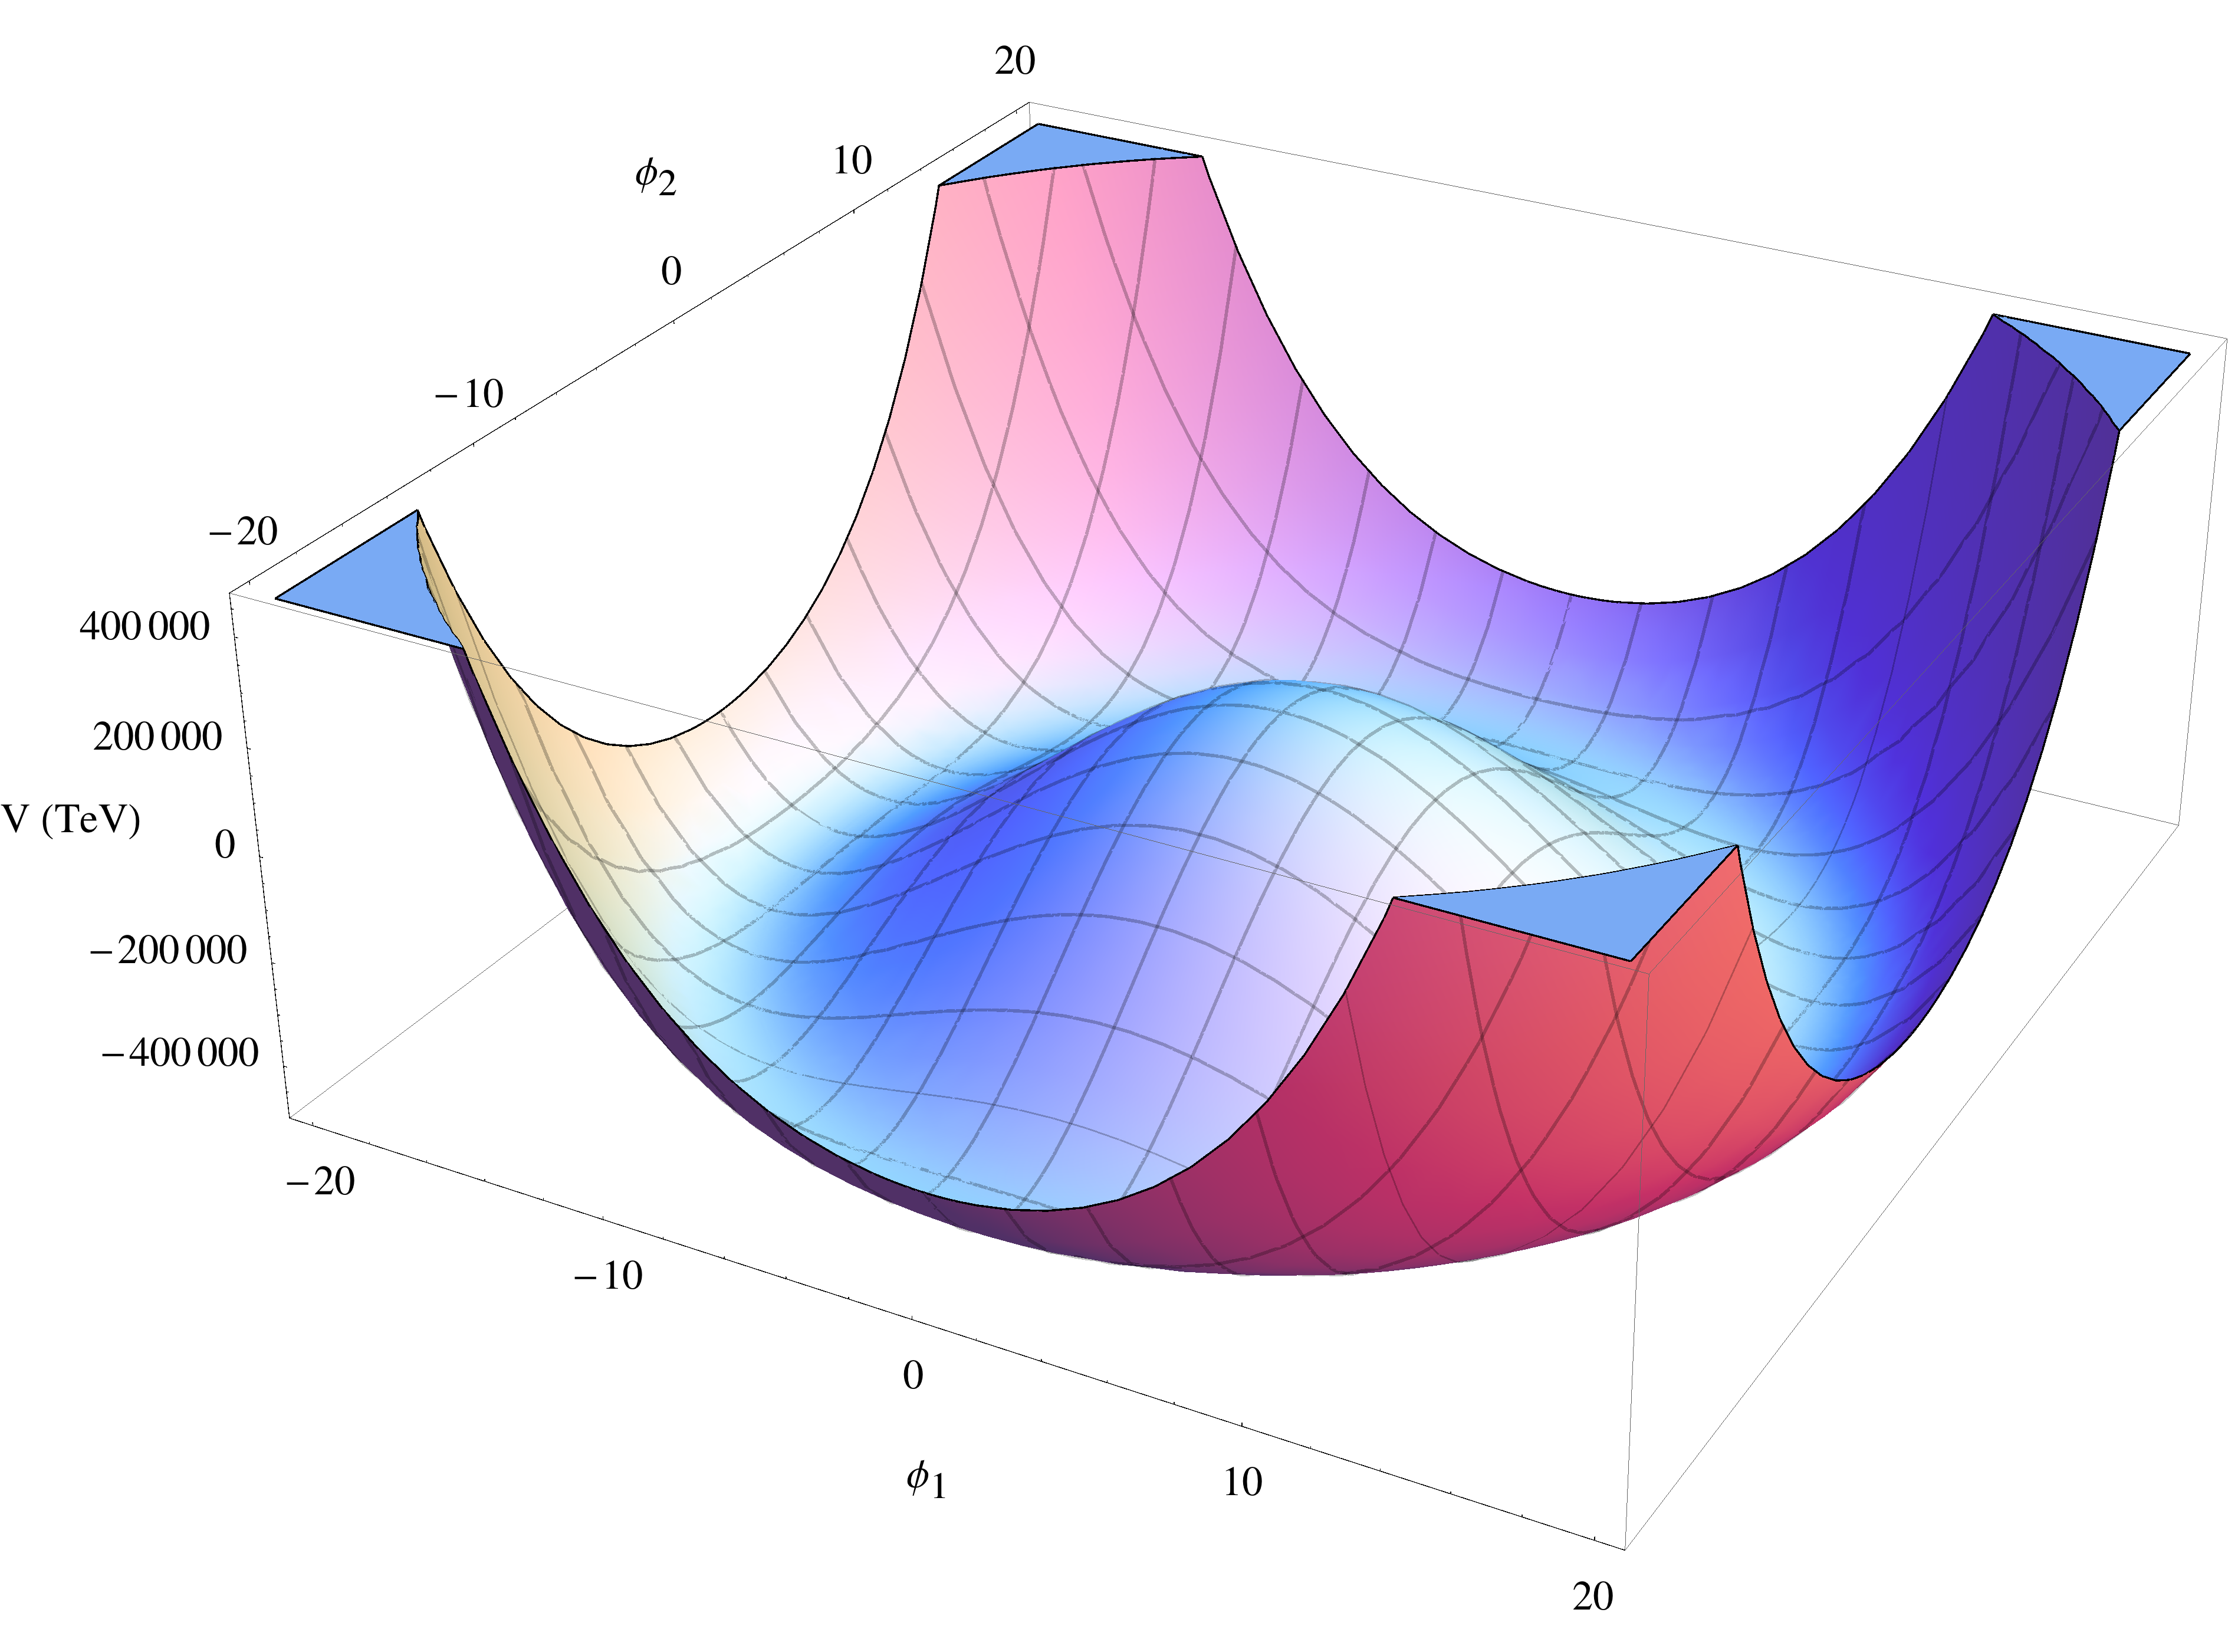
\includegraphics[width=0.6\linewidth]{Higgs_potential.png}
  \caption{Le potentiel de Higgs tracé avec les valeurs de $\mu^2$ et $\lambda$ calculées pour $m_{h} = \SI{125.3}{\GeVc}$}
\end{figure}

\subsection{Le mécanisme de Higgs}

Nous sommes intéressés par un mécanisme qui nous permet d'introduire une masse pour les médiateurs de l'interaction faible. On brise la symétrie $SU(2)_L \times U(1)_Y$ en introduisant un champ scalaire, doublet d'isospin, interagissant avec les quatre champ vectoriels $\vec{W}_\mu$ et $B_\mu$. On ajoute ainsi un terme $\mathcal{L}_2$ au Lagrangien $\mathcal{L}_\text{EWK}$ \eqref{eq:l_ewk}
\begin{align} \label{eq:l_higgs_ewk}
  \mathcal{L}_2 &= \left( \dmu \phi \right)^\star \left( \dmu \phi \right) - V(\phi)
\end{align}

On impose l'invariance locale de jauge sous une transformation de $SU(2)_L \times U(1)_Y$
\begin{align*}
  \phi \rightarrow e^{i\vec{\theta}(x) \cdot \vec{T}\,+\,i\iota(x) Y} \phi
\end{align*}

Cette invariance introduit les quatre champs vectoriels de l'interaction électrofaible. En procédant de façon identique aux sections précédentes, on obtient
\begin{align*}
  \mathcal{L}_2 &= \left| \left( i \dmu - g_1 \frac{1}{2} \vec{\tau} \cdot \vec{W}_\mu - g_2 \frac{Y}{2} B_\mu \right) \phi \right|^2 - V(\phi)
\end{align*}

On choisit comme champ scalaire un doublet d'isospin d'hypercharge $Y = 1$
\begin{align*}
 \phi &= \colvec{2}{\phi^+}{\phi^0} \quad \text{avec} \quad \begin{aligned}
    \phi^+ &= \frac{1}{\sqrt{2}} ( \phi_1 + i \phi_2 ) \\
    \phi^0 &= \frac{1}{\sqrt{2}} ( \phi_3 + i \phi_4 )
  \end{aligned}
\end{align*}

$V(\phi)$ est le potentiel de Higgs, qui admet comme minimum
\begin{align*}
  \frac{1}{2} ( \phi_1^2 + \phi_2^2 + \phi_3^2 + \phi_4^2 ) = - \frac{\mu^2}{2\lambda}
\end{align*}

Sans perte de généralité, on choisit un minimum défini par
\begin{align*}
  \phi_1 = \phi_2 = \phi_4 = 0, \quad \phi_3^2 = v^2 = - \frac{\mu^2}{2\lambda}
\end{align*}

On réexprime le champ scalaire par son expansion autour du minimum
\begin{align*}
  \phi(x) = \frac{1}{\sqrt{2}} \colvec{2}{0}{v + \eta(x) + i \frac{\vec{\tau}}{2} \cdot \vec{\xi}(x) } \simeq \frac{1}{\sqrt{2}} \exp{\left[i\frac{\vec{\tau} \cdot \vec{\xi}(x)}{2v}\right]} \colvec{2}{0}{v + \eta(x)} 
\end{align*}

En injectant $\phi$ dans le Lagrangien, on fait apparaître un terme de masse pour chacun des champs $\vec{W}_\mu$ et $B_\mu$, un terme de masse pour le champ scalaire $\eta$, mais aussi trois nouveaux champs scalaires non massif $\vec{\xi}$. Cependant, on voit aussi apparaître des termes de la forme $\dmu \xi W^\mu$ et $\dmu \xi B^\mu$. En terme d'interaction, ces termes correspondent à
\begin{center} \begin{fmfgraph*}(180,30)
  \fmfleft{i1} \fmfright{o1}
  \fmf{scalar,label=$\xi$}{i1,v1}
  \fmf{boson,label=$W$}{v1,o1}
  \fmfdot{v1}
\end{fmfgraph*} \end{center}
et suggèrent que nous n'avons pas correctement identifié les particules fondamentales dans le Lagrangien. Celui ci étant invariant de jauge, nous sommes libre de choisir n'importe quelle jauge pour l'exprimer, et en particulier une jauge qui permet d'obtenir $\vec{\xi} = \vec{0}$. En remplaçant $\eta$ par $h$, on choisit comme transformation
\begin{align*}
  \phi(x) \rightarrow \frac{1}{\sqrt{2}} e^{i\vec{\theta}(x) \cdot \vec{T}\,+\,i\iota(x) Y} \colvec{2}{0}{v + h(x)}
\end{align*}

Pour conserver l'invariance par transformation de jauge locale, les champs $\vec{W}_\mu$ et $B_\mu$ se transforment maintenant de façon à faire disparaître les champs scalaires $\vec{\xi}$! Il ne reste plus que le champ scalaire $h(x)$ dans le Lagrangien: c'est le champ de Higgs.

\bigskip

Afin d'obtenir les termes de masse associés aux champs $\vec{W}_\mu$, on remplace dans le Lagrangien \eqref{eq:l_higgs_ewk} $\phi$ par sa valeur au minimum 
\begin{align*}
  \phi(x) = \frac{1}{\sqrt{2}} \colvec{2}{0}{v}
\end{align*}

On obtient alors
\begin{align*}
&\left| \left( - g_1 \frac{1}{2} \vec{\tau} \cdot \vec{W}_\mu - g_2 \frac{1}{2} B_\mu \right) \phi \right|^2 \\
& \quad = \frac{1}{8} \left| \begin{pmatrix}
  - g_1 W^3_\mu - g_2 B_\mu & -g_1 \left( W^1_\mu -i W^2_\mu \right) \\
  -g_1 \left( W^1_\mu + i W^2_\mu \right) &  g_1 W^3_\mu - g_2 B_\mu 
\end{pmatrix} \colvec{2}{0}{v} \right|^2 \\
& \quad = \left( \frac{1}{2} v g_1 \right)^2 W^+_\mu W^{- \mu} + \frac{1}{8} v^2 \rowvec{2}{W^3_\mu}{B_\mu} \begin{pmatrix}
   g_1^2 & - g_1 g_2 \\
   - g_1 g_2 & g_2^2
 \end{pmatrix} \colvec{2}{W^3_\mu}{B_\mu} 
\end{align*}

Le premier terme est le terme de masse des bosons chargés, $W^{\pm}$. On a
\begin{align*}
  M_{W^{\pm}} &= \frac{1}{2} v g_1
\end{align*}

Le dernier terme contient les champs $W^3_\mu$ et $B_\mu$. On a vu précédemment que ces champs ne peuvent pas être interprétés comme les bosons $Z^0$ et $\gamma$, puisque $W^3$ ne couple que des particules d'hélicité gauche. Cependant, on constate que ce terme comporte des éléments non diagonaux : le mécanisme de Higgs fait apparaître naturellement un mélange entre les champs $W^3_\mu$ et $B_\mu$ pour donner naissance aux champs $Z_\mu$ et $A_\mu$.
\begin{align*}
  \frac{1}{8} v^2 \rowvec{2}{W^3_\mu}{B_\mu} \begin{pmatrix}
   g_1^2 & - g_1 g_2 \\
   - g_1 g_2 & g_2^2
 \end{pmatrix} \colvec{2}{W^3_\mu}{B_\mu} &= \frac{1}{8} v^2 \left( g_1W^3_\mu - g_2 B_\mu \right)^2 + 0 \left( g_2 W^3_\mu + g_1B_\mu \right) \\
 &= \frac{1}{8} v^2 \left(g_1^2 + g_2^2\right) Z_\mu^2 + 0 A_\mu^2
\end{align*}
avec
\begin{align*}
  Z_\mu &= \frac{g_1W^3_\mu - g_2 B_\mu}{\sqrt{g_1^2 + g_2^2}} & & & A_\mu &= \frac{g_2W^3_\mu + g_1 B_\mu}{\sqrt{g_1^2 + g_2^2}} \\  
\end{align*}

Le terme de masse d'un boson vecteur neutre étant de la forme $\frac{1}{2} M_V^2 V_\mu^2$, on identifie
\begin{align*}
  M_Z &= \frac{1}{2} v \sqrt{g_1^2 + g_2^2} & & & M_A &= 0
\end{align*}

L'introduction d'un nouveau champ scalaire se couplant  à $\vec{W_\mu}$ et à $B_\mu$ permet, grâce au mécanisme de Higgs, de générer une masse pour les médiateurs de l'interaction faible, tout en gardant le photon non massif. On peut réexprimer le mélange entre $W^3_\mu$ et $B_\mu$ en introduisant l'angle de mélange $\theta_W$ (angle de Weinberg), et en posant
\begin{align*}
  \frac{g_2}{g_1} &= \tan \theta_W
\end{align*}

On obtient alors
\begin{align} \label{eq:ewk_mixing}
  \colvec{2}{A_\mu}{Z_\mu} &= \begin{pmatrix}
    \cos \theta_W & \sin \theta_W \\
    - \sin \theta_W & \cos \theta_W
  \end{pmatrix} \colvec{2}{B_\mu}{W^3_\mu}
\end{align}
et
\begin{align*}
  \frac{M_W}{M_Z} &= \cos \theta_W
\end{align*}

Connaissant maintenant l'existence d'un mélange entre les bosons $W^3_\mu$ et $B_\mu$, on peut injecter \eqref{eq:ewk_mixing} dans \eqref{eq:l_ewk}. En ne considérant que la partie neutre du Lagrangien, on obtient
\begin{align*}
  \mathcal{L}_{\text{neutre}} &= \bar{\chi}_L \gmuc \left( -g_1 T^3 W^3_\mu -g_2 \frac{Y}{2} B_\mu \right) \chi_L + \Psib_R \gmuc \left(-g_2 \frac{Y}{2} B_\mu \right) \Psi_R \\
  &\begin{aligned} =\ &\bar{\chi}_L \gmuc \left( \left\{ -g_1 T^3 \sin\theta_W -g_2 \frac{Y}{2} \cos\theta_W \right\} A_\mu \right. \\
                     +&\hphantom{\bar{\chi}_L \gmuc \left(\vphantom{\frac{Y}{2}}\right.} \left. \left\{ -g_1 T^3 \cos\theta_W + g_2 \frac{Y}{2} \sin\theta_W \right\} Z_\mu \right) \chi_L\\
                     +&\Psib_R \gmuc \left( \left\{-g_2 \frac{Y}{2} \cos\theta_W\right\}A_\mu + \left\{ g_2 \frac{Y}{2} \sin\theta_W \right\} Z_\mu \right) \Psi_R
                     \end{aligned}
\end{align*}

On sait que le couplage au photon, obtenu grâce au Lagrangien QED \eqref{eq:l_qed}, est de la forme $e Q A_\mu$. En utilisant la relation \eqref{eq:q_t_y}, on trouve que les couplages $g_1$ et $g_2$ doivent satisfaire la relation suivante
\begin{align*}
  g_1 \sin\theta_W = g_2 \cos\theta_W = e
\end{align*}

Les couplages de l'interaction électrofaible ne sont pas indépendant, et sont reliés à la charge électrique.

\subsection{Champ de Higgs et masses des fermions}

On a vu précédemment que le champ scalaire introduit présentait un minimum de potentiel obtenu pour une valeur $\phi \neq 0$. On réexprime donc $\phi$ par une expansion autour de son minimum $v$
\begin{align*}
  \phi(x) = \frac{1}{\sqrt{2}} \colvec{2}{0}{v + h(x)}
\end{align*}

En injectant $\phi$ dans le potentiel $V(\phi)$, on obtient
\begin{align*}
  V(\phi) &= \frac{1}{4} v^2\mu^2 - \mu^2h^2 - \frac{\mu^2}{v} h^3 + \frac{1}{4} \lambda h^4
\end{align*}

Le champ de Higgs est donc massif, et on a $m_h = \sqrt{-\mu^2} = \sqrt{2v^2 \lambda}$, nouveau paramètre libre de la théorie. Les deux derniers termes représentent l'interaction du champ de Higgs avec lui même (à trois et quatre vertex). On dit qu'il est auto-couplant.

\bigskip

Dans le Lagrangien électrofaible \eqref{eq:l_ewk}, le terme de masse des fermions n'a pas pu être inclus puisqu'il brisait l'invariance locale de jauge. En effet, si on considère le terme $m\Psib\Psi$, on a
\begin{align*}
  m \Psib \Psi &= m \Psib \left[ \frac{1}{2} \left(1 - \gfivec\right) + \frac{1}{2} \left(1 + \gfivec\right) \right] \Psi \\
  &= m \left[ \Psib_R \Psi_L + \Psib_L \Psi_R \right]
\end{align*}

Ce terme dépend donc à la fois des composantes de chiralité gauche et droite du champ. Hors, ces quantités ne se transforment pas de la même façon sous une transformation $SU(2)_L \times U(1)_Y$ : l'invariance est brisée.

Il s'avère que le même doublet de Higgs peut aussi générer la masse des fermions du Modèle Standard. On procède de façon analogue à la section précédent, et on introduit dans le Lagrangien un terme invariant sous $SU(2)_L \times U(1)_Y$ :
\begin{align*}
  \mathcal{L}_3 &= -G_f \left[ \rowvec{2}{\bar{\nu}}{\bar{f}}_L \phi f_R + \bar{f}_R \phi^\dagger \colvec{2}{\nu}{f}_L \right] \qquad f = e, \mu, \tau
\end{align*}

On substitue $\phi$ par son expansion autour du minimum, et on obtient
\begin{align*}
  \mathcal{L}_3 &= -\frac{G_f}{\sqrt{2}} v (\bar{f}_L f_R + \bar{f}_R f_L) -\frac{G_f}{\sqrt{2}} v (\bar{f}_L f_R + \bar{f}_R f_L)h
\end{align*}

Les leptons acquièrent donc une masse $m_f = \frac{G_f v}{\sqrt{2}}$. Le dernier terme représente quant à lui l'interaction des leptons avec le champ de Higgs, avec un couplage proportionnel à la masse. On introduit donc trois nouveaux paramètres libres dans la théorie, un pour chaque fermion : ce sont les couplages de Yukawa des leptons au champ de Higgs.

Intéressons nous maintenant aux quarks. Leur masse est générée de façon identique, à une différence près : il faut un moyen de générer une masse pour les quarks de type \emph{up} qui, contrairement aux neutrinos, ont une masse. On introduit un nouveau doublet de Higgs $\phi_C$, qui se transforme de façon identique à $\phi$, et qui se couple aux quarks de type \emph{up}
\begin{align*}
  \phi_C &= -i \tau_2 \phi^\star = \colvec{2}{- \bar{\phi}^0}{\phi^-} \xrightarrow[\text{brisure de symétrie}]{} \frac{1}{\sqrt{2}} \colvec{2}{v + h}{0}
\end{align*}

Le nouveau terme à insérer dans le Lagrangien est
\begin{align*}
  \mathcal{L}_4 &= -G_d^{ij} \rowvec{2}{\bar{u}_i}{\bar{d}_i^\prime} \colvec{2}{\phi^+}{\phi^0} d_{jR} - G_u^{ij} \rowvec{2}{\bar{u}_i}{\bar{d}_i^\prime} \colvec{2}{- \bar{\phi}^0}{\phi^-} u_{jR} + \text{conjugué hermitien}
\end{align*}

On substitue $\phi$ par son expansion autour du minimum, et on obtient
\begin{align*}
  \mathcal{L}_4 &= - m_d^i \bar{d}_i d_i \left( 1 + \frac{h}{v} \right) - m_u^i \bar{u}_i u_i \left( 1 + \frac{h}{v} \right)
\end{align*}

Comme pour le cas des fermions, on introduit six nouveaux paramètres libres dans la théorie, un pour chaque quark.

\bigskip

\begin{figure}
  \subcaptionbox{\label{fig:higgs_mgg}}[.45\linewidth]{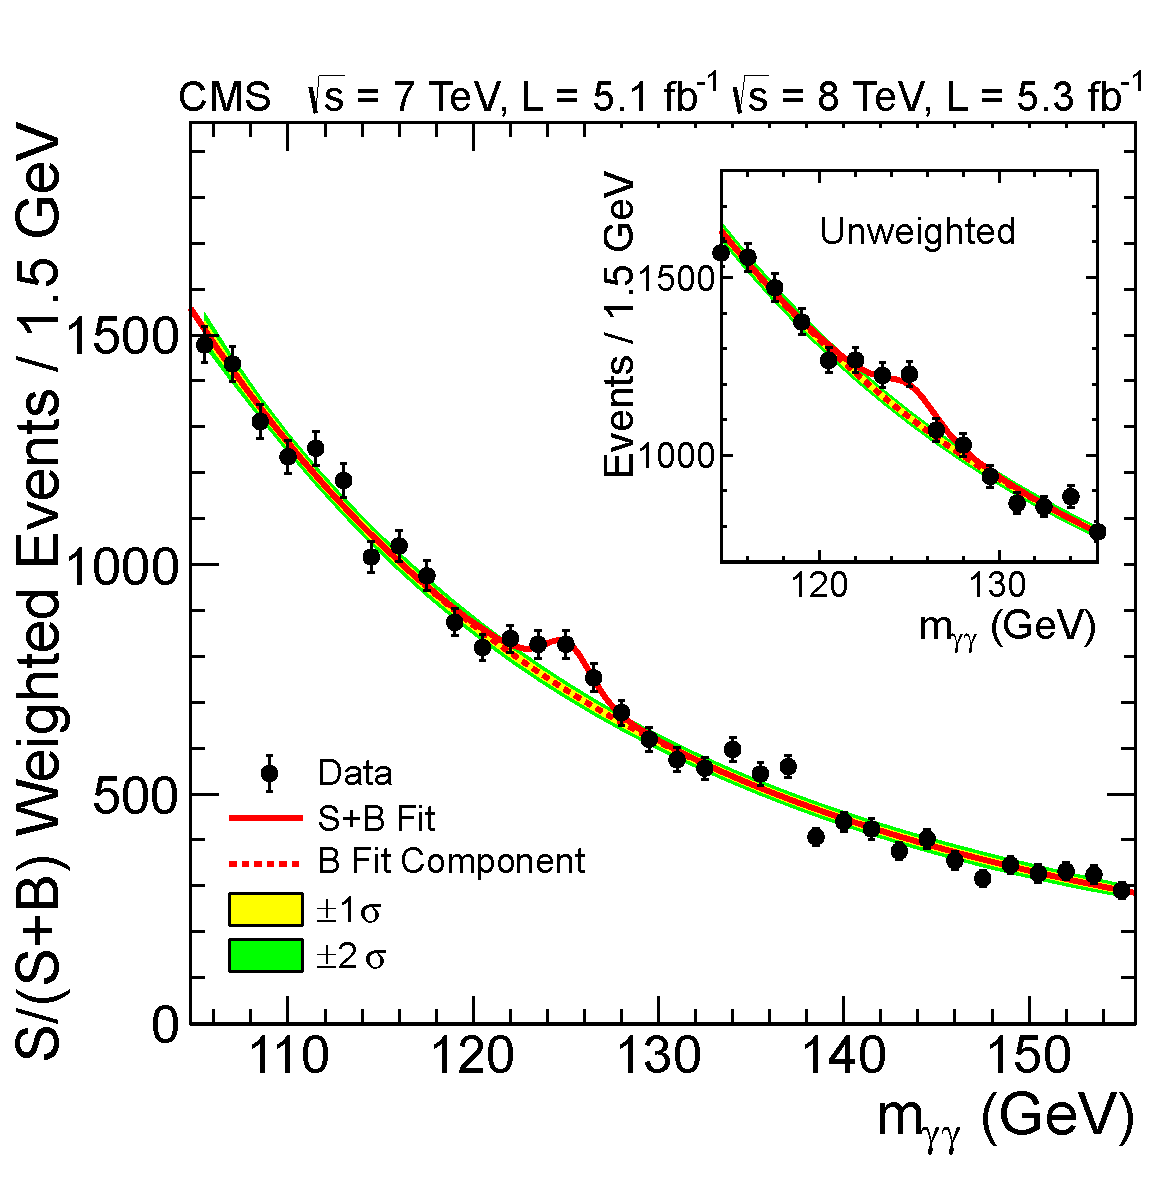
\includegraphics[width=0.45\textwidth]{higgs_mgg.pdf}}\hfill
  \subcaptionbox{\label{fig:higgs_pvalue}}[.45\linewidth]{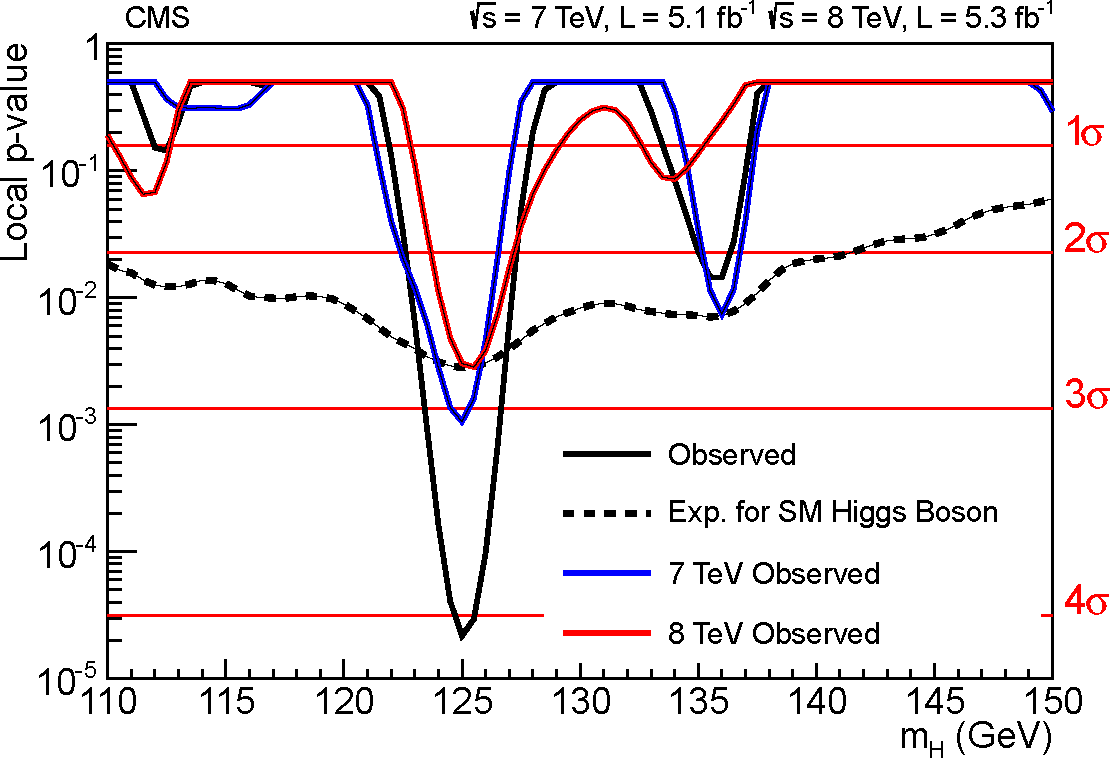
\includegraphics[width=0.45\textwidth]{higgs_pvalue.pdf}}
  \caption{A gauche, spectre de masse invariante $H \rightarrow m_{\gamma\gamma}$. A droite, la \emph{p-value} associée à cette mesure, qui correspondant à la probabilité que la mesure soit compatible avec une absence de signal. On voit clairement la présence d'une nouvelle particule aux alentour de \SI{125}{\GeV}.}
\end{figure}

Au travers de la brisure de symétrie et du mécanisme de Higgs, on a pu voir comment les bosons de jauges $W$ et $Z$, les leptons et les quarks acquièrent une masse.
\begin{itemize}
  \item Les masses des bosons de jauge faible s'exprime à l'aide de $\mu^2$ et $\lambda$, les paramètres du potentiel de Higgs.
  \item Les masses des fermions deviennent des paramètres libres de la théorie.
\end{itemize}

Le mécanisme de Higgs prévoit donc l'existence d'un nouveau champ scalaire, le champ de Higgs. Le boson associé a une masse $m_h = \sqrt{2v^2\lambda}$. Plus de 30 ans après sa prédiction, le CERN a officiellement annoncée le 4 juillet 2012 la découverte d'une nouvelle particule compatible avec le boson de Higgs \citep{higgs_cms,higgs_atlas}. Cette particule a été observée dans plusieurs canaux de désintégrations, dont $H \rightarrow \gamma\gamma$ et $H \rightarrow ZZ$. On peut voir figure \ref{fig:higgs_mgg} le spectre de masse invariante $m_{\gamma\gamma}$ pour l'expérience CMS, où on voit clairement une déviation par rapport à la prédiction théorique, et figure \ref{fig:higgs_pvalue} la \emph{p-value} associée à la découverte. La \emph{p-value} représente la probabilité que la mesure soit compatible avec une absence de signal. On remarque la très nette déviation autour de \SI{125}{\GeV}.

% Des signes sont aussi présent dans la désintégration $\tau\tau$, ce qui serait la preuve qu'il est en effet correct d'étendre le mécanisme de Higgs pour générer la masse des fermions.
Selon les derniers résultats, ce boson a une masse de $m_h = \SI{125.9 \pm 0.4}{\GeV}$ \citep{pdg}. De nombreuses recherches sont encore en cours afin de déterminer si ce boson est bien celui prédit par le Modèle Standard, mais les premiers résultats laissent à penser que c'est le cas.

% \subsection{Renormalisation} \label{sec:renormalisation}

% Lorsque l'on ajoute des boucles aux diagrammes d'un processus à l'arbre, le calcul de l'élément de matrice de transition diverge. Par exemple, lors du passage du diagramme \ref{fig:ee_annihilation} au diagramme \ref{fig:ee_annihilation_high_order}, il est nécessaire d'intégrer sur toutes les impulsions possibles, puisque la particule qui forme la boucle est virtuelle. Ceci entraîne l'apparition de terme de la forme $\int k dk$, avec $k \rightarrow \infty$. termes qui divergent.

% \begin{figure}[t] \centering
%   \subcaptionbox{\label{fig:ee_annihilation}}[.4\linewidth]{
%   \begin{fmfgraph*}(180,100)
%     \fmfpen{0.5}
%     \fmfleft{i1,i2}
%     \fmfright{o1,o2}
%     \fmf{fermion}{i1,v1,i2}
%     \fmf{fermion}{o1,v2,o2}
%     \fmfdot{v1} \fmfdot{v2}
%     \fmf{photon,label=$\gamma$}{v1,v2}
%     \fmflabel{$e^-$}{i1} \fmflabel{$e^+$}{i2} 
%     \fmflabel{$e^+$}{o1} \fmflabel{$e^-$}{o2} 
%   \end{fmfgraph*}}\qquad%
% %   \subcaptionbox{\label{fig:ee_annihilation_high_order}}[.4\linewidth]{
% %   \begin{fmfgraph*}(180,100)
% %     \fmfpen{0.5}
% %     \fmfleft{i1,i2}
% %     \fmfright{o1,o2}
% %     \fmf{fermion}{i1,g1,v1,g2,i2}
% %     \fmf{fermion,tension=0.5}{o1,v2,o2}
% %     \fmfdot{v1} \fmfdot{v2}
% %     \fmf{photon,label=$\gamma$}{v1,v2}
% %     \fmf{photon,label=$\gamma$,tension=0,left=0.7}{g1,g2}
% %     \fmflabel{$e^-$}{i1} \fmflabel{$e^+$}{i2} 
% %     \fmflabel{$e^+$}{o1} \fmflabel{$e^-$}{o2} 
% %   \end{fmfgraph*}}
%   \subcaptionbox{\label{fig:ee_annihilation_high_order}}[.4\linewidth]{
%   \begin{fmfgraph*}(180,100)
%     \fmfpen{0.5}
%     \fmfleft{i1,i2}
%     \fmfright{o1,o2}
%     \fmf{fermion}{i1,v1,i2}
%     \fmf{fermion}{o1,v2,o2}
%     \fmfdot{v1} \fmfdot{v2}
%     \fmf{photon,label=$\gamma$,tension=2}{v1,g1}
%     \fmf{photon,label=$\gamma$,tension=2}{g2,v2}
%     \fmf{fermion,left=1,label=$e^-$}{g1,g2}
%     \fmf{fermion,left=1,label=$e^+$}{g2,g1}
%     \fmflabel{$e^-$}{i1} \fmflabel{$e^+$}{i2} 
%     \fmflabel{$e^+$}{o1} \fmflabel{$e^-$}{o2} 
%   \end{fmfgraph*}}
%   \caption{Diagrammes de Feynman $e^+e^- \rightarrow e^+e^-$ d'ordre 1 (\protect\subref{fig:ee_annihilation}) et d'ordre 2 (\protect\subref{fig:ee_annihilation_high_order}).}
%   \label{fig:ee_annihilation_total}
% \end{figure}

% Néanmoins, il est possible de supprimer ces divergences en introduisant un \emph{cut-off} dans la théorie, c'est-à-dire une énergie arbitraire jusqu'où le modèle est valide. Ce nouveau paramètre est ensuite absorbé dans une redéfinition de la constante de couplage du processus, qui par conséquence n'est plus constante mais dépend de l'énergie du processus : c'est la renormalisation.

% \bigskip

% Pour l'interaction électromagnétique, la constante de couplage $\alpha_0$ devient, après renormalisation
% \begin{align*}
%   \alpha\left(Q^2\right) &= \frac{\alpha(\mu^2)}{1 - \frac{\alpha(\mu^2)}{2\pi} \ln\left( \frac{Q^2}{\mu^2} \right) }
% \end{align*}
% où $Q^2$ est l'énergie à laquelle évaluer la constante de couplage, et $\mu^2$ la valeur de l'échelle de renormalisation.

% Dans le cas de l'interaction forte, la constante de couplage $\alpha_s$ devient
% \begin{align*}
%   \alpha_s\left(Q²\right) &= \frac{\alpha_s(\mu^2)}{1 + \frac{\alpha_s(\mu^2)}{12\pi} \left(33 - 2n_f\right) \ln\left( \frac{Q^2}{\mu^2} \right) }
% \end{align*}
% où $n_f$ est le nombre de saveurs (6 quarks). Une chose importante à noter est que la constante de couplage de l'interaction forte \emph{diminue} avec l'énergie, and devient faible pour des faibles distances d'interaction : c'est la liberté asymptotique. A l'inverse, plus la distance d'interaction augmente, plus l'interaction est importe : à partir d'une certaine distance, l'énergie disponible est suffisante pour créer une paire $q\bar{q}$. Il n'est ainsi pas possible d'observer un quark seul, c'est le confinement.

% On définit une nouvelle échelle, $\Lambda^2$, définit comme la valeur à laquelle la constante de couplage devient trop importante pour que le calcul perturbatif puisse être utilisé. On a
% \begin{align*}
%   \Lambda^2 &= \mu^2 \exp\left( \frac{-12\pi}{(33 - 2n_f) \alpha_s\left(\mu^2\right)} \right) \\
%   \alpha_s\left(Q^2\right) &= \frac{12 \pi}{\left(33 - 2n_f\right) \ln\left( \frac{Q^2}{\Lambda^2} \right)}
% \end{align*}

% On peut voir $\Lambda$ comme la frontière entre le monde des quarks libres, décrit correctement par des calculs perturbatifs, et le monde des quarks liés. Afin de décrire ces états, les calculs perturbatifs ne sont pas correct, la constante de couplage étant grande devant l'unité. On peut utiliser des techniques de simulation telle que la QCD sur réseau \citep{PhysRevD.10.2445}.

\section{Faiblesses du Modèle Standard} \label{sec:sm_weakness}

Depuis son développement dans les années 1960, le Modèle Standard est un succès expérimental. Il a en effet prédit l'existence des bosons $W^{\pm}$, $Z$, des quarks $b$ et $t$ avant leur découverte. Si l'on exclu la récente découverte d'une particule compatible avec le boson de Higgs en 2012, la dernière découverte est celle du quark $t$ en 1995 au Tevatron, l'accélérateur de particule du FNAL, aux États-Unis. On présente figure \ref{fig:ewk_fit} les derniers résultats de l'ajustement des paramètres de la théorie électrofaible. En effet, le Modèle Standard permet de relier quasiment tous les paramètres par des relations. L'ajustement permet donc de comparer directement les prédictions du Modèle Standard avec les mesures expérimentales. Les différences entre les valeurs expérimentales et les valeurs ajustées sont toutes inférieures à 3 $\sigma$, démonstration du succès du Modèle Standard.

Malgré ce succès qui dure depuis plus de 50 ans, un certain nombre d'interrogations et de problèmes demeurent. En effet, un certain nombre d'éléments laissent à penser que le Modèle Standard n'est qu'un modèle effectif à baisse énergie d'une théorie plus fondamentale.

\begin{figure} \centering
  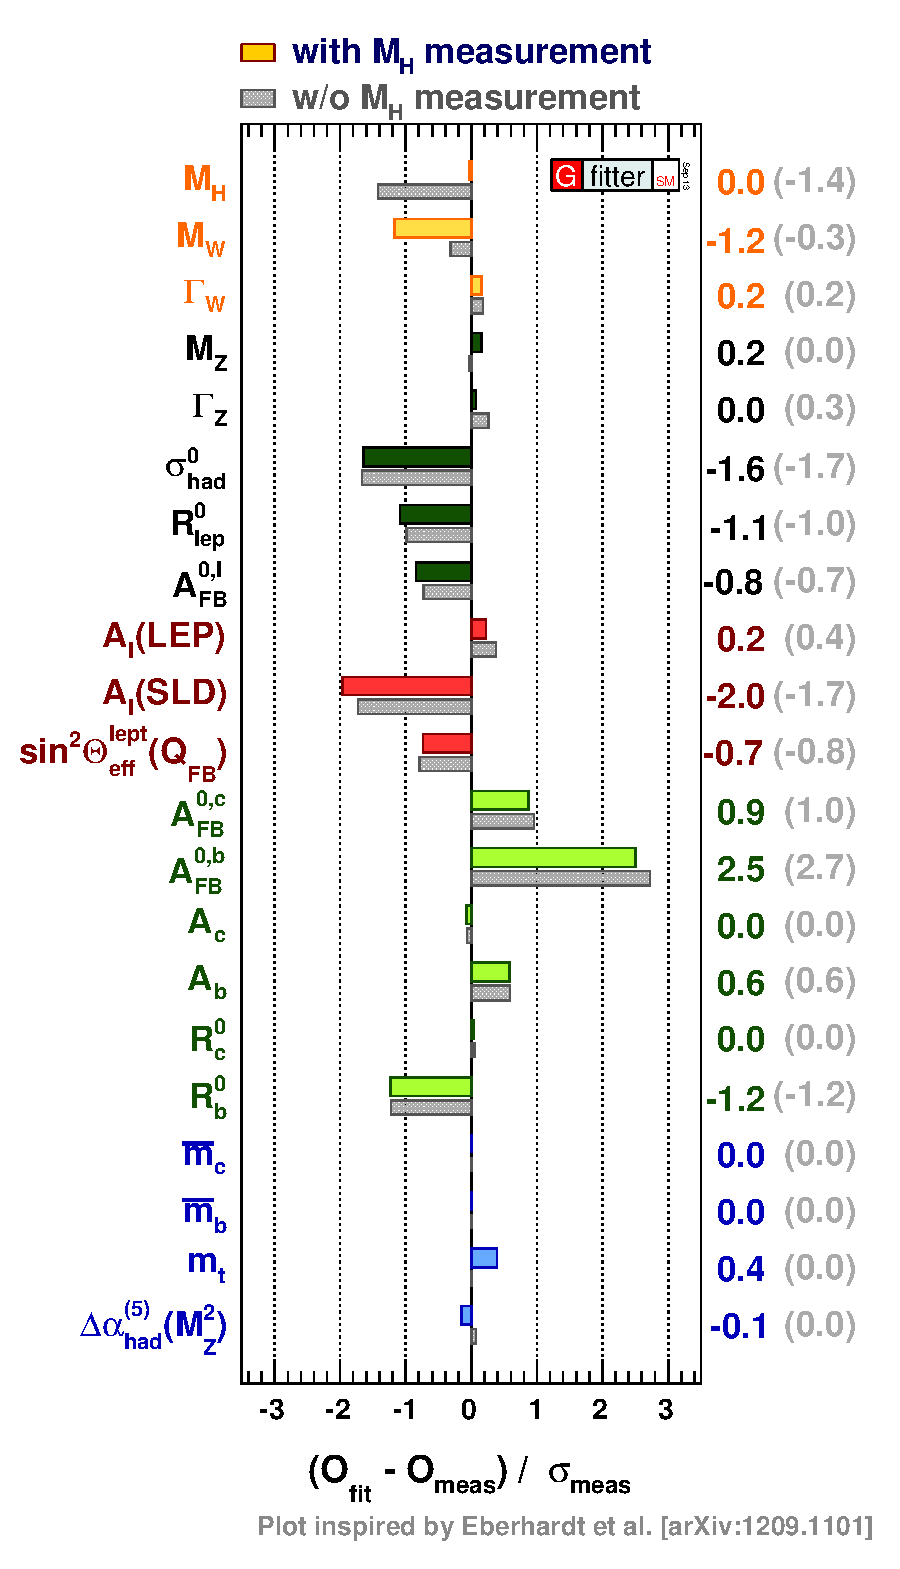
\includegraphics[height=0.9\textheight]{PullPlotTwoBarsCol_logo.eps}
  \caption{Comparaison entre les valeurs expérimentales et les valeurs ajustées des principales observables de la théorie électrofaible du Modèle Standard, pour deux cas de figures : en couleurs, l'ajustement inclut la découverte du probable boson de Higgs ; en gris, ce résultat n'est pas utilisé. Les valeurs à droite correspondent au \emph{pull}, c'est-à-dire à la différence entre la valeur expérimentale et la valeur ajustée, exprimée en sigma, où 1$\sigma$ correspond à un intervalle de confiance de \SI{68.2}{\%}. Les faibles écarts observés ($<$ à 3 $\sigma$) sont une démonstration du succès du Modèle Standard. Résultats issus de \citep{ewk_fit}.}
  \label{fig:ewk_fit}
\end{figure}

\begin{description}
  \item[Nombre de paramètres libres] Tel que construit, le Modèle Standard comporte 19 paramètres libres : les 6 masses des quarks, les 3 masses des leptons, l'angle de mélange électrofaible, les 4 paramètres de la matrice CKM, les 3 constantes de couplage, et les deux paramètres du potentiel de Higgs. L'un des objectifs majeur de la Physique étant de décrire de façon la plus simple possible les phénomènes, tout laisse à penser qu'une théorie comportant moins de paramètres libres engloberait le Modèle Standard.
  \item[Nombre de générations] Les contraintes sur le nombre de générations de leptons proviennent des mesure de la largeur du $Z$, et conduisent à une prédiction de 3 générations. Néanmoins, une quatrième génération plus massive que la masse du $Z$ ou non couplée à l'interaction faible n'est pas exclue ; le Modèle Standard ne prédit pas le nombre de générations de fermions.
  \item[L'ajustement fin] Les diagrammes de Feynman qui contribuent au calcul de la masse du boson de Higgs incluent des boucles, qui conduisent à des divergences. Le Modèle Standard étant une théorie renormalisable, ces divergences peuvent être absorbées dans la masse du boson, conduisant à une masse effective ($m_h$) différente de la masse nue ($m_{h, 0}$) \citep{higgs_mass} :
  \begin{align*}
    m_h^2 &= m_{h, 0}^2 - \frac{3 \Lambda^2}{8 \pi^2 v^2} \left(m_h² + 2m_W^2 + m_Z^2 - 4m_t\right)
  \end{align*}
  où $\Lambda$ est le \emph{cut-off} (la limite haute de l'intégrale). Si on considère le Modèle Standard valide jusqu'à l'échelle de la grande unification ($\Lambda = \SI{\tilde e16}{\GeV}$), et un boson de Higgs avec $m_h = \SI{125}{\GeV}$, il est nécessaire de procéder à un ajustement jusqu'à la vingtième décimale entre la masse nue du boson et les corrections radiatives. Cet ajustement fin suggère l'existence d'autres processus qui viendraient naturellement annuler ces corrections radiatives.
  \item[Quantification de la charge électrique] On sait par l'expérience que la charge électrique est quantifiée, et doit être un multiple de $e = \SI{1.602176565(35)}{\coulomb}$ ($1$ pour les leptons, $\sfrac{1}{3}$ pour les quarks). L'opérateur de charge $Q$ est introduit afin de reproduire cette quantification, mais aucune justification théorique n'est donnée dans le cadre du le Modèle Standard.
\begin{figure} \centering
  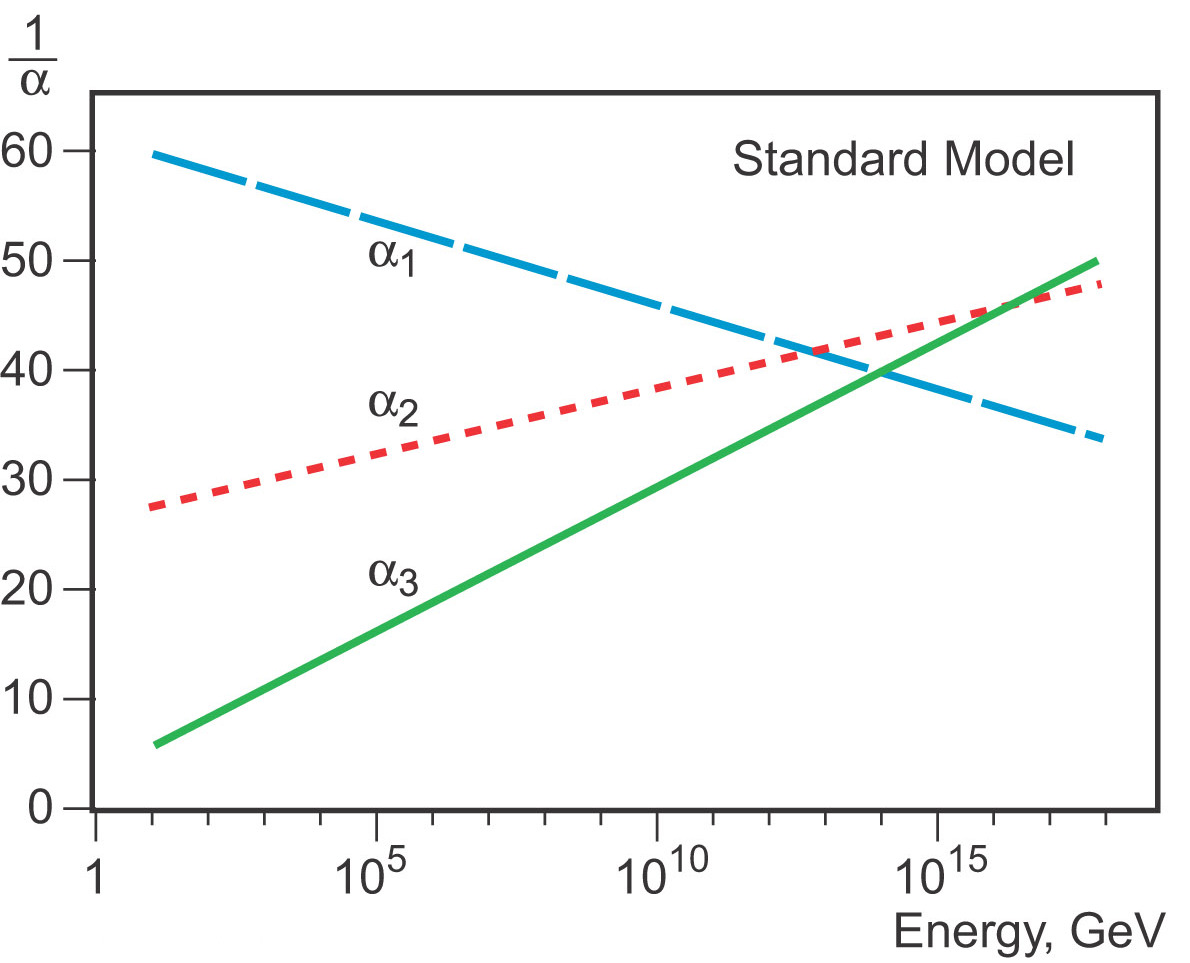
\includegraphics[width=0.5\linewidth]{running_coupling.jpg}
  \caption{L'évolution des constantes de couplages du Modèle Standard en fonction de l'énergie. On remarque qu'à une certaine énergie, les constantes de couplages semblent être identique : un signe d'une possible unification des interactions ?}
  \label{fig:unification}
\end{figure}
  \item[Grande unification] On peut voir figure \ref{fig:unification} l'évolution des constantes de couplage en fonction de l'énergie. Ces constantes semblent tendre à s'unifier à une certain énergie, ce qui pourrait indiquer une possible unification entre les trois interactions. De nombreux modèles au-delà du Modèle Standard modifient les couplages de façon à ce que les trois interactions se croisent en un unique point.
  \item[Neutrinos] Le Modèle Standard que l'on vient de bâtir prévoit des neutrinos sans masse. La découverte de l'oscillation des neutrinos (\tilde 1970 avec la découverte de l'oscillation des neutrinos solaires) impose néanmoins aux neutrinos d'être massif. De façon analogue aux quarks, il est possible d'inclure dans le Modèle Standard un terme supplémentaire afin de permettre aux neutrinos d'acquérir une masse grâce au mécanisme de Higgs. Il reste cependant à expliquer pourquoi il existe une telle différence de masse entre les leptons et les neutrinos (\SI{511}{\keV} contre \SI{\tilde 1}{\eV}). La solution pourrait venir du mécanisme de \emph{see-saw}. En effet, l'existence de neutrinos massifs impose l'existence de neutrinos de chiralité droite. Si on postule que ces neutrinos droits sont des particules de Majorana\footnote{Une particule de Majorana est une particule étant sa propre anti-particule.}, il est possible d'ajouter au Lagrangien, en plus du terme de masse de Higgs, un nouveau terme de masse, invariant sous une transformation $SU(2)_L \times U(1)_Y$, de la forme :
\begin{align*}
  \mathcal{L} &= \frac{-M}{2} \left[ \left(\nu_R^C\right)^\dagger \nu_R + \nu_R^\dagger \nu_R^C \right] \\
              &= \frac{-M}{2} \left[ \nu_R^\dagger \nu_R + \nu_R \nu_R^\dagger \right]
\end{align*}
où l'exposant $C$ correspondant à la conjugaison de charge. En combinant ce terme avec celui obtenu par le mécanisme de Higgs, on trouve
\begin{align*}
  \mathcal{L} &= \rowvec{2}{\nu_L^\dagger}{\nu_R^\dagger} \begin{pmatrix}
    0 & m_D\\
    m_D & M
  \end{pmatrix} \colvec{2}{\nu_L}{\nu_R}
\end{align*}
où $m_D$ est la masse obtenue grâce au mécanisme de Higgs, et $M$ grâce au terme de Majorana. Afin d'obtenir les états propres de masse, on diagonalise la matrice. Les valeurs propres sont
\begin{align*}
  m_1 &\simeq \frac{m_D^2}{M} &&& m_2 &\simeq M
\end{align*}
  
  Si on choisi comme valeur pour $m_D$ une valeur proche de la masse des fermions, et une valeur très grande pour $M$, on voit que l'on génère deux masses : une très faible, $m_1$, qui serait la masse des neutrinos gauches, et une très grande, $m_2$, qui serait la masse d'un hypothétique neutrino droit.
  
% Les neutrinos étant massif, il existe forcément des neutrinos de chiralité droite. N'ayant jamais été observés, ces neutrinos semblent insensible aux trois interactions fondamentales du Modèle Standard : il ne porte ainsi aucune charge électrique, de couleur ou faible. On peut donc considérer le neutrino droit comme une particule de Majorama, c'est-à-dire une particule étant sa propre anti-particule. Dans ce cas, il est possible d'inclure dans le Lagrangien un terme de masse invariant sous transformation de jauge locale, de la forme

\medskip
  
L'oscillation des neutrinos peut elle être expliquée de manière analogue au mélange entre les quarks. On introduit une nouvelle matrice de mélange entre les neutrinos états propres de masse et les neutrinos états propre de l'interaction faible : la matrice PMNS \citep{neutrino_mixing_1,neutrino_mixing_2}. Cette matrice est paramétrisée par trois angles de mélange et une phase. Les dernières valeurs expérimentales \citep{pdg} sont
    \begin{align*}
      \theta_{12} \simeq  \SI{34}{\degree}, \theta_{23} \simeq \SI{45}{\degree}, \theta_{13} \simeq \SI{9.1}{\degree} 
    \end{align*}
    la phase $\delta CP$ n'ayant pas encore été mesurée.
  
%   Il reste cependant à expliquer pourquoi la masse des neutrinos est si faible comparée à celle des autres leptons. En effet, les limites expérimentales pose une limite supérieure sur la masse des neutrinos \citep{pdg} de $\SI{2}{\eV}$ pour $\nu_e$, $\SI{0.19}{\MeV}$ pour $\nu_\mu$ et $\SI{18.2}{\MeV}$ pour $\nu_\tau$.
  
  \item[Gravitation] Le Modèle Standard unit sous un même formalisme mathématique les interactions électromagnétiques, faible et forte. La gravitation est elle décrite par la relativité générale. A l'échelle de grande unification, l'interaction gravitionnelle devient du même ordre de grandeur que les autres interactions et ne peut plus être négligée : une nouvelle théorie est alors nécessaire tenant compte de la gravité.
  
  De nombreuses tentatives ont eu lieu pour quantifier la gravitation. Elles se heurtent toutes au même problème : une fois intégrée à la théorie, celle-ci n'est plus renormalisable et conduit à des probabilités infinies. Néanmoins, les recherches continuent, et la théorie la plus prometteuse est actuellement la théorie des supercordes, qui permet d'unifier sous un même formalisme les quatre interactions fondamentales, en considérant les particules fondamentales non pas comme des particules, mais comme des cordes vibrantes.
\end{description}

% \begin{figure} \centering
%   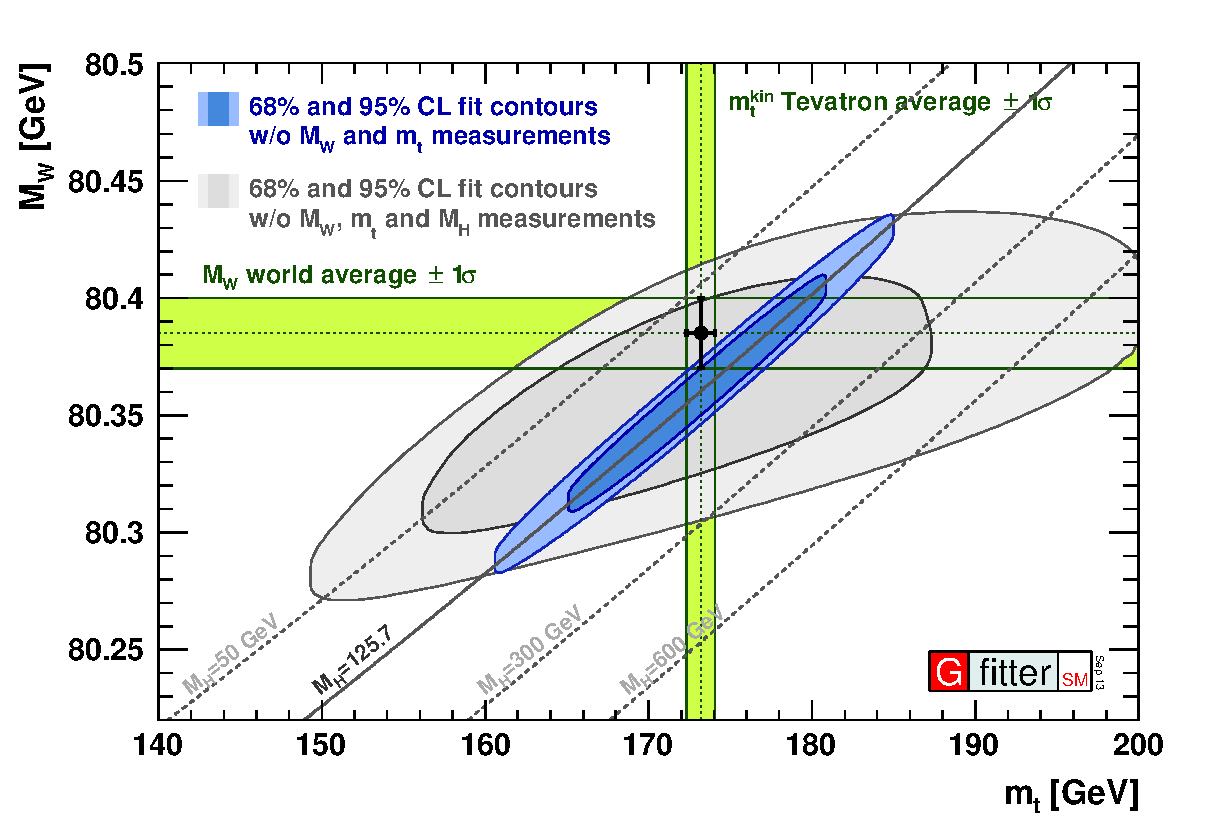
\includegraphics[width=0.55\linewidth]{W_vs_top_logo.eps}
%   \caption{Contour du fit des paramètres électrofaible du Modèle Standard en fonction de $m_t$ et $m_W$. Les valeurs expérimentales de $m_t$ et $m_W$ sont en jaune. Le contour gris n'inclue pas la valeur de $m_h = \SI{125.7}{\GeV}$ dans le fit, à la différence du contour bleue. Les prédictions théoriques sont en accord avec l'expérience.}
%   \label{fig:ewk_w_vs_top}
% \end{figure}

% \begin{figure} \centering
%   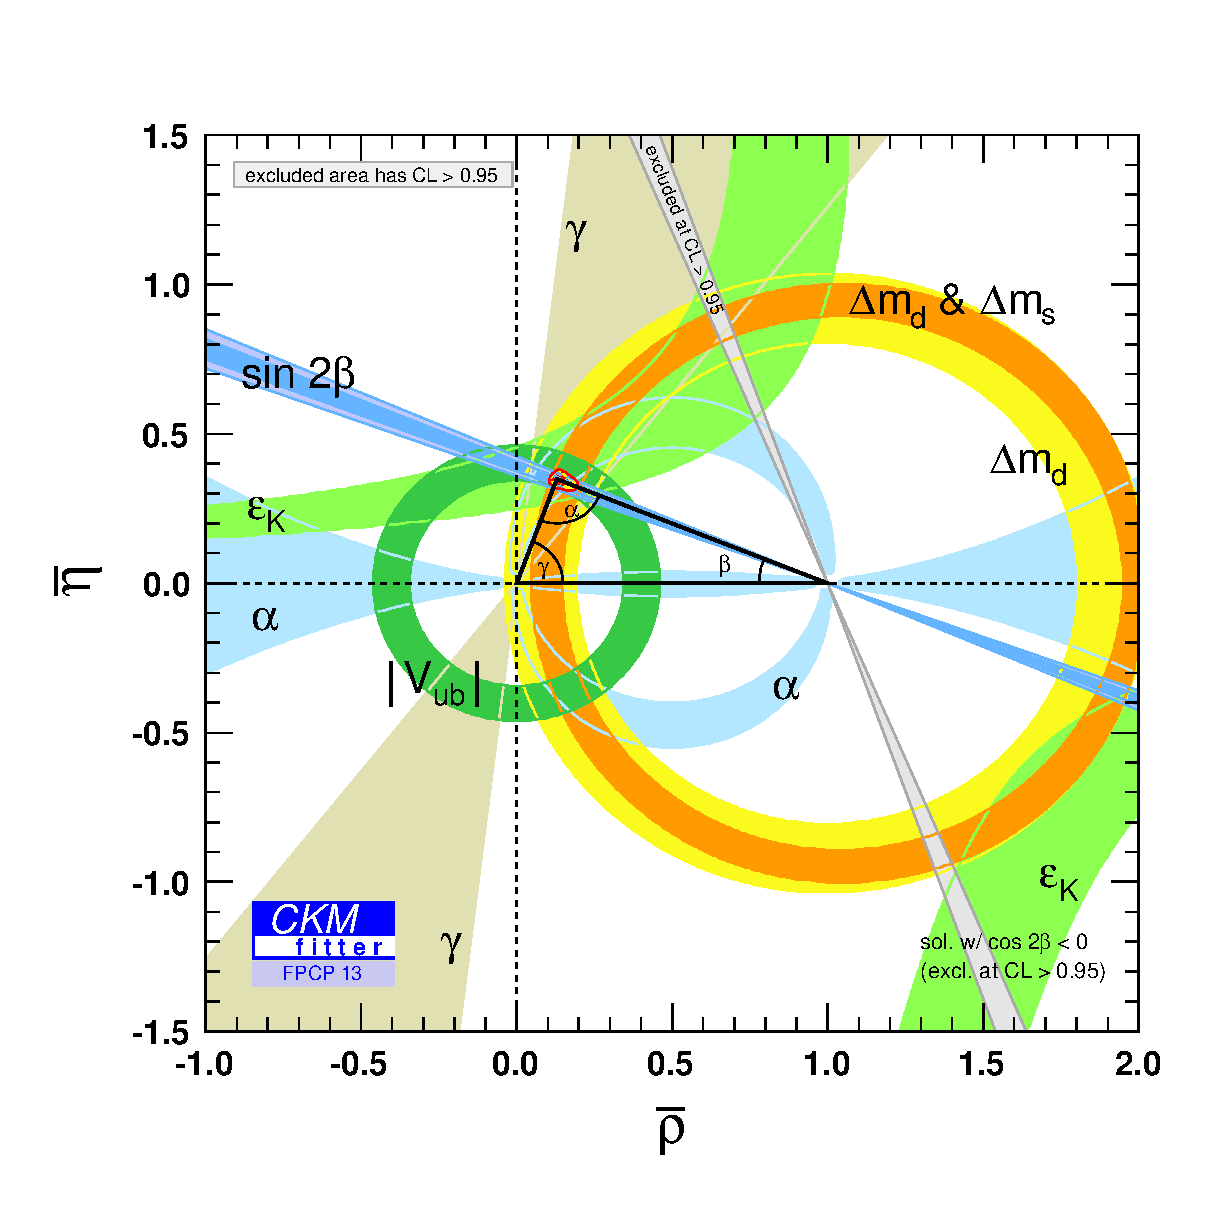
\includegraphics[width=0.55\linewidth]{ckm_triangle.eps}
%   \caption{Triangle d'unitarité de la matrice CKM. REFERENCE}
%   \label{fig:ckm_triangle}
% \end{figure}

\section{Conclusion}

On a vu au cours de ce chapitre comment a été construit le Modèle Standard. Fort de nombreuses prédictions et de la récente découverte d'un boson compatible avec le boson de Higgs par le CERN, le Modèle Standard est plus que jamais un succès théorique. Néanmoins, de nombreux arguments laissent penser que le Modèle Standard n'est qu'une théorie effective d'une théorie plus simple et plus globale.

\bigskip

Il existe de nombreuses théories au-delà du Modèle Standard permettant de résoudre les faiblesses du modèle. Ces théories prédisent de nouvelles particules, de nouveaux bosons voire de nouvelles dimensions. Il est donc important pour les expérimentateurs de disposer d'outils adaptés permettant de vérifier les prédictions de ces nombreuses théories. C'est le cas du \emph{Large Hadron Collider} (\emph{LHC}, grand collisionneur de hadrons), dont la description détaillée est l'objet du prochain chapitre.

\end{fmffile}

\cleardoublepage\chapter{Dispositif expérimental} \label{chap:detecteur}

%\section{Les accélérateurs de particules}

La particule élémentaire la plus massive du Modèle Standard est le quark top, avec une masse d'environ \SI{173}{\GeV}. Si l'on souhaite explorer des zones où peuvent se trouver de la nouvelle physique, il faut être en mesure de pouvoir générer des particules beaucoup plus massive, et donc fournir une grande quantité d'énergie. On utilise pour cela des accélérateurs de particules, qui permettent de faire collisionner deux particules accélérées à grande énergie dans le but de produire d'autres particules beaucoup plus massives.

On distingue deux grandes classes d'accélérateurs de particules, chacune avec ses avantages et ses défauts : les accélérateurs linéaires et les accélérateurs circulaires.

\begin{itemize}
  \item Les accélérateurs linéaires accélèrent les particules en ligne droite. L'énergie atteinte étant proportionnelle à la longueur d'accélération, ces accélérateurs sont souvent limités en énergie. Leur principale force vient de l'absence de rayonnement synchroton lors de l'accélération, ce qui permet d'utiliser des électrons pour les collisions tout en atteignant des énergies élevés. Les électrons étant des particules fondamentales, les signatures expérimentales des collisions sont extrêmement claires, ce qui permet d'effectuer des mesures de précisions.
  \item Les accélérateurs circulaires accélèrent les particules le long d'un anneau. Les particules effectuant plusieurs tours, la montée en énergie est considérable. Il est néanmoins nécessaire de courber la trajectoire des particules pour obtenir cette trajectoire circulaire, ce qui cause l'apparition de rayonnement synchroton. Pour garder une énergie importante, il faut donc utiliser des particules très massives, telles que des protons. Les signatures expérimentales des collisions deviennent alors plus compliquées, puisque plusieurs partons peuvent participer à la collision.
\end{itemize}

Traditionnellement, on dénomme les accélérateurs circulaires des accélérateurs à découverte, puisqu'il est possible, avec une même énergie dans le centre de masse, de balayer toute une zone en énergie. En effet, les hadrons n'étant pas des particules élémentaires, les partons participant à la collision emportent une certaine fraction de l'impulsion disponible. On fixe donc une borne supérieure à l'énergie disponible, mais pas de borne inférieure. Au contraire, les accélérateurs linéaires sont eux des machines de précisions. Grâce à leur environnement propre, il est possible d'étudier très précisément des phénomènes particuliers, par exemple ceux découvert dans un accélérateur circulaire.

\section{Le Large Hadron Collider (LHC)}

Le grand collisionneur de hadrons est à ce jour le plus grand et le plus puissant accélérateur de particules au monde. Il est installé en lieu et place du LEP (\emph{Large Electron Positron collider}), dans un tunnel de \SI{27}{\km} de circonférence, enfoui à plus de \SI{100}{\m} au dessous de la surface. Géographiquement, le LHC est situé à la frontière Franco-Suisse, sur le site du CERN (Organisation Européenne pour la Recherche Nucléaire).

Composé de deux anneaux, le LHC permettra d'accélérer des protons à des énergies de \SI{7}{\TeV} (\SI{14}{\TeV} dans le centre de masse), grâce à 16 cavités radio-fréquence, et maintenu le long d'une trajectoire circulaire par environ 9500 aimants. Refroidis à une température de \SI{1.8}{\K} grâce à de l'hélium super fluide, ces aimants supraconducteurs délivrent un champ magnétique nominal de \SI{8.33}{\tesla}.

Le premier faisceau a circulé au LHC le 10 septembre 2008. Malheureusement, le 19 septembre 2008, un incident de cryogénie entraînât une interruption de plus d'un an, et ce n'est que le 20 novembre 2009 que les anneaux du LHC accueillirent de nouveau des protons. A partir du 23 novembre, les premières collisions $pp$ destinées à la physique ont commencé à être enregistrées par les détecteurs. S'en suivirent 3 années de montée en puissance progressive, passant d'une énergie de \SI{7}{\TeV} dans le centre de masse en 2010-2011 à \SI{8}{\TeV} en 2012. Au moment de la rédaction de ce manuscrit, le LHC est arrêté pour environ 2 ans. Cet arrêt planifié permet de préparer le LHC au passage à \SI{14}{\TeV}. Il est aussi mis à profit afin de mettre à jour légèrement les détecteurs. Les collisions $pp$ pour la physique devraient reprendre en avril 2015.

\subsection{L'accélération des protons}
Avant d'atteindre leur énergie nominale dans l'anneau du LHC, les protons sont accélérés graduellement le long de différents accélérateurs :

\begin{figure} \centering
  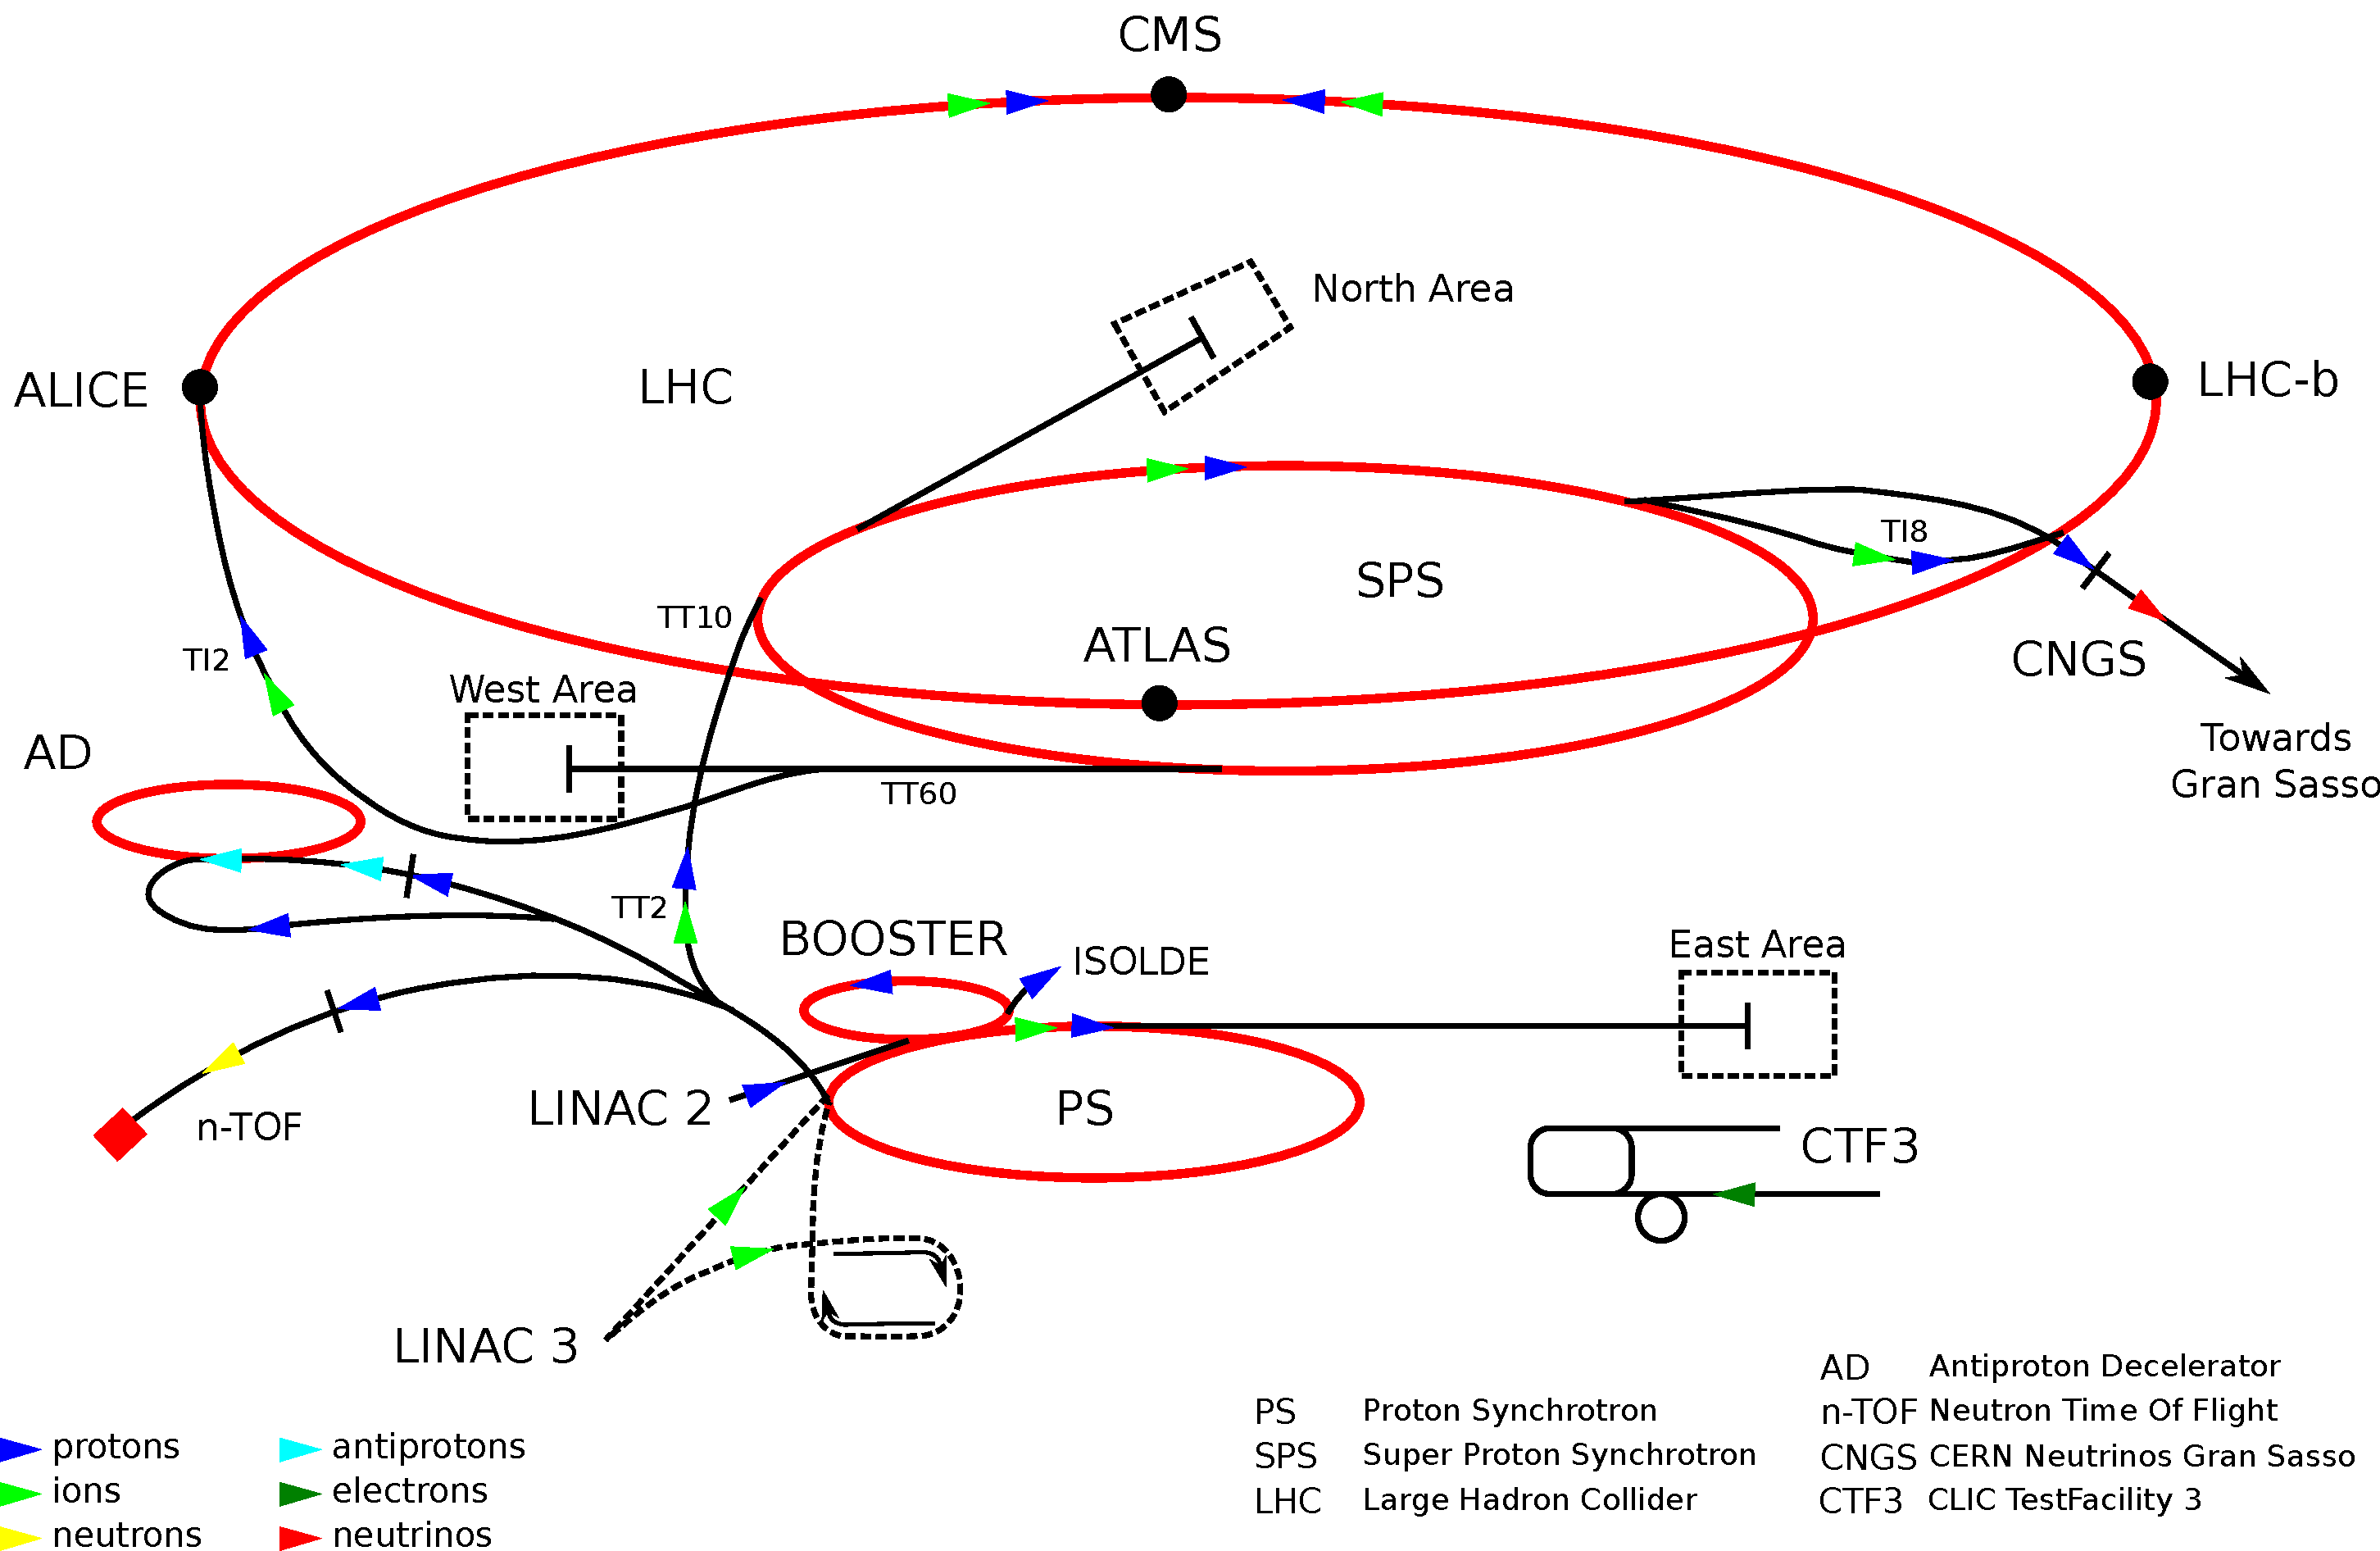
\includegraphics[width=0.7\textwidth]{Cern-accelerator-complex.pdf}
  \caption{Le complexe d'accélérateurs du CERN}
  \label{fig:lhc_complex}
\end{figure}

\begin{description}
  \item[Le LINAC 2 (1978)] Tout commence par une simple bouteille d'hydrogène. Un champ électrique ionise le gaz afin d'arracher les électrons du noyau. Les protons restant sont accélérés jusqu'à une énergie de \SI{50}{\MeV}.
  \item[Le \emph{Proton Synchroton Booster} (PSB -- 1972)] Le faisceau est ensuite injecté dans le PSB, un accélérateur circulaire, où les protons atteignent une énergie de \SI{1.4}{\GeV}.
  \item[Le \emph{Proton Synchroton} (PS -- 1959)] Dans cet accélérateur, les protons atteignent une énergie de \SI{25}{GeV}.
  \item[Le \emph{Super Proton Synchroton} (SPS -- 1976)] Le faisceau subit sa dernière étape d'accélération dans le SPS, atteignant cette fois ci une énergie de \SI{450}{\GeV}, avant d'être injecté dans le LHC et accéléré pour atteindre l'énergie nominale de \SI{7}{\TeV} par faisceau.
  %\item[Le LHC] L'énergie du faisceau est suffisante pour atteindre l'anneau du LHC. Il est cette fois accéléré jusqu'à l'énergie nominale.
\end{description}

Un schéma descriptif de la chaîne d'accélération du CERN est présenté figure \ref{fig:lhc_complex}

\subsection{La luminosité}

La luminosité instantanée est une variable clé d'un accélérateur de particule. Exprimée en \si{\per\square\cm\per\second}, elle est proportionnelle au nombre de collisions par seconde et par centimètre carré. On l'exprime au LHC en fonction de diverses variables caractéristiques de la forme des paquets de protons,
de l'énergie, de la séparation des paquets, etc. On a
\begin{align*}
  \mathcal{L}_{\text{inst}} &= \frac{\gamma\,f\,n_p\,N_p^2}{4\pi\,\epsilon_n\,\beta^*} = \frac{f\,n_p\,N_p^2}{4\pi\,\sigma_x\,\sigma_y}
\end{align*}
où $\gamma$ est le boost de Lorentz, $f$ la fréquence de révolution des paquets, $n_p$ le nombre de paquets de protons, $N_p$ le nombre de protons par paquets, $\epsilon_n$ l'émittance transverse\footnote{L'émittance est une mesure du parallélisme du faisceau.}, $\beta^*$ la fonction d'amplitude\footnote{Afin de favoriser les collisions $pp$, les deux faisceaux sont rapprochés l'un de l'autre autour du point du collision. $\beta^*$ mesure la distance entre le point d'interaction et l'endroit où le faisceau double de largeur.} et $\sigma_{x,y}$ les tailles transverses du faisceau au point d'interaction. Les valeurs des différents paramètres du faisceau sont donnés table \ref{tab:lhc_beam} pour les trois années de fonctionnement.

\begin{figure} \centering
  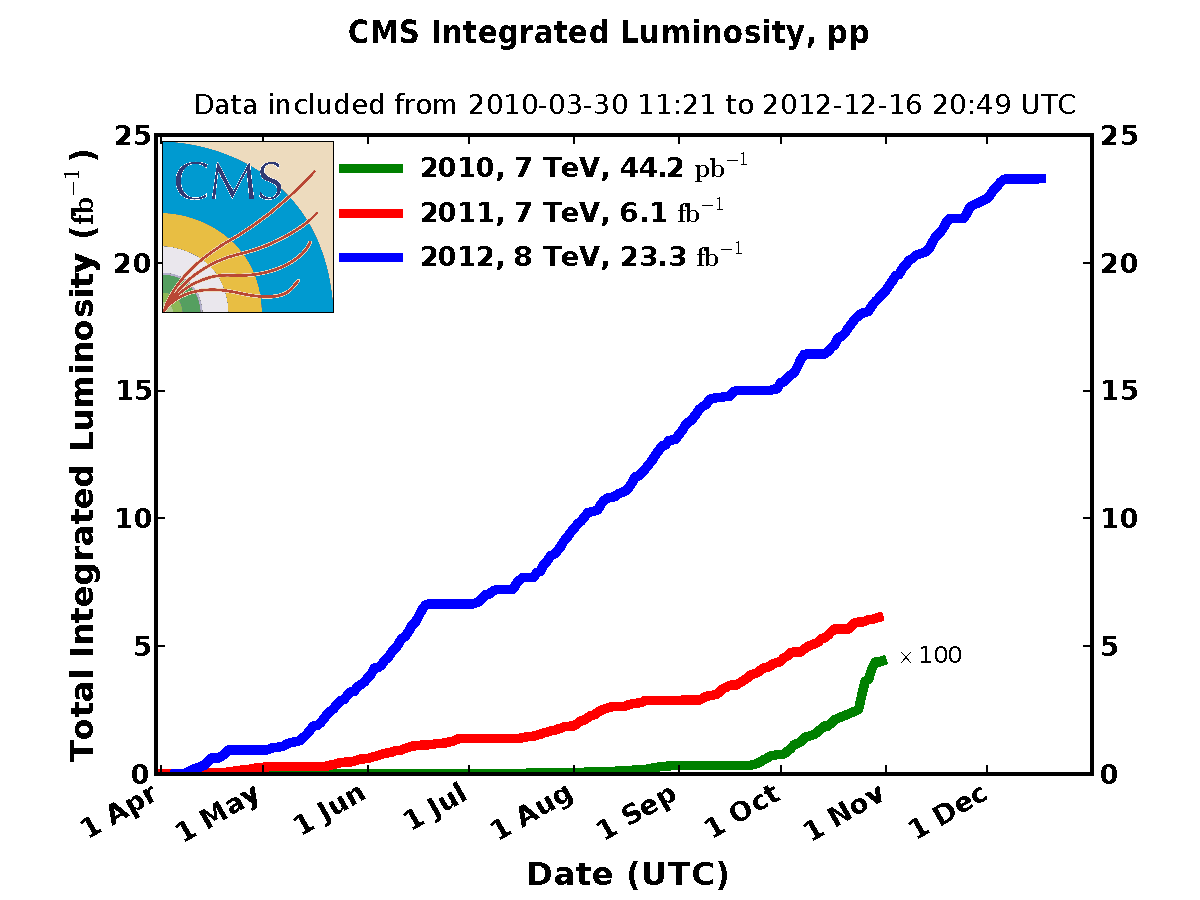
\includegraphics[width=0.7\textwidth]{chapitre2/figs/CMS_lumi.pdf}
  \caption{Luminosité intégrée collectée par l'expérience CMS au cours des années 2010 (vert), 2011 (rouge) et 2012 (bleu). La distribution de la luminosité collectée a été zoomé 100x pour pouvoir la distinguer sur le graphique.}
  \label{fig:lumi}
\end{figure}

\begin{table} \centering
  \begin{tabular}{@{}ccccc@{}} \toprule
  \multirow{2}{*}{Caractéristiques} & \multicolumn{4}{c}{Conditions} \\ \cmidrule{2-5}
  & nominales & 2010 & 2011 & 2012 \\ \midrule
  Énergie par faisceau (\si{\TeV}) & 7 & \num{3.5} & \num{3.5} & \num{4} \\
  $\mathcal{L}_\text{inst}$ (\si{\per\square\cm\per\s}) & \num{e34} & \num{2.1e32} & \num{3.7e33} & \num{7.7e33}\\
  $\mathcal{L}$ (\si{\invfb}) & 100 & \num{36e-3} & \num{4.98} & \num{19.7} \\ \midrule
  Temps entre paquet (\si{\ns}) & 25 & > 150 & 75 / 50 & 50 \\
  Nombre de paquets & 2808 & 368 & 1092 & 1380\\
  Protons par paquets (\num{e11}) & \num{1.15} & \num{1.2} & \num{1.45} & \num{1.7}\\
  $\beta^*$ (\si{\m}) & \num{0.55} & \num{2.0} - \num{3.5} & \num{1.0} - \num{1.5} & \num{0.6} \\ \bottomrule
  \end{tabular}
  \caption{Les différents paramètres du faisceau $pp$ du LHC pour les trois premières années de fonctionnement}
  \label{tab:lhc_beam}
\end{table}

\medskip

On obtient la luminosité totale en intégrant $\mathcal{L}_{\text{inst}}$ sur la durée de prise de données, $\mathcal{L} = \int \mathcal{L}_\text{inst}\,dt$. C'est grâce à cette luminosité que l'on quantifie la quantité de données disponible (statistique) pour les expériences. En effet, le nombre d'événements produit par les collisions pour un processus donné est
\begin{align*}
  N &= \mathcal{L} \sigma
\end{align*}
où $\sigma$ est la section efficace du processus. On voit donc que pour une section efficace donnée, le nombre d'événements produit est directement proportionnel à la luminosité. Il est donc primordial d'avoir une luminosité instantanée la plus grande possible et une durée de prise de données la plus longue possible afin d'être en mesure d'observer des processus rare. On peut voir figure \ref{fig:lumi} la distribution de la luminosité collectée par l'expérience CMS (section \ref{sec:cms}) au cours de 3 années de prise de données.

\bigskip

Bien qu'opérant actuellement à des énergies presque deux fois plus faible que celles prévues par les conditions nominales, le LHC est déjà capable de fournir une luminosité instantanée pic équivalente à celle sensée être obtenue à \SI{14}{\TeV}. Cela laisse présager d'excellentes performances lors de la reprise en 2015.

\subsection{L'empilement}

Lors d'un croisement de paquets de protons, plusieurs interactions $pp$ peuvent avoir lieu : la collision principale forme l'événement dur, et c'est celle ci qu'on souhaite étudier. Les autres collisions (élastiques ou inélastiques) viennent parasiter la collision principale, et se superposent à l'événement dur. Cet effet est communément appelé empilement (\pu (PU) en anglais). Le nombre d'événements de PU par collision dépend de la configuration du LHC. En 2012, on l'estime à environ 21, et il est prévu qu'il passe à environ 40 lors de la reprise en 2015.

\medskip

On distingue deux types d'empilement différent : celui produit en même temps que l'événement dur est le plus handicapant, puisqu'il va entraîner de l'activité non désirée au sein du détecteur, et ainsi perturber la reconstruction des particules produites lors de la collision principale. C'est le PU "in-time". On distingue aussi le PU "out-of-time", principalement causé par le temps de réponse des détecteurs. Lors de collisions intenses, il est possible que les détecteurs soient toujours occupés à traiter un événement alors qu'une autre collision survient, produisant alors une superposition des deux événements pendant un court instant.

\subsection{Les expériences}

Le LHC étant un collisionneur circulaire, il est possible de faire se croiser les faisceaux de protons à plusieurs endroits. On peut donc installer plusieurs dispositifs expérimentaux, un à chaque point de croisement. Le LHC compte 4 points de croisements, et donc 4 expériences majeures : ALICE \citep{alice}, ATLAS \citep{atlas}, CMS \citep{cms} et LHCb \citep{lhcb}.

\begin{description}
  \item[A Large Ion Collider Experiment (ALICE)] Cette expérience est principalement dédiée à l'étude du déconfinement de la matière nucléaire, le plasma de quark et gluon. Les données qu'elle utilise sont celles issues des collisions d'ions lourds ($Pb-Pb$ ou $p-Pb$), mais les collisions $pp$ sont aussi utilisées afin de calibrer le détecteur.
  \item[A Toroidal LHC ApparatuS (ATLAS) / Compact Muon Solenoid (CMS)] Ce sont les deux expériences généralistes du LHC. En effet, le programme de physique de ATLAS et CMS est très vaste, et couvre la recherche du boson de Higgs et de nouvelle physique, les mesures de précisions du Modèle Standard, ainsi que la recherche de candidats matière noire. Souvent mises en concurrence, ces expériences sont pourtant complémentaires. Ainsi, on a pu voir le 4 juillet 2012 ces deux expériences annoncer conjointement la découverte d'une particule compatible avec le boson de Higgs \citep{higgs_atlas,higgs_cms}, chacune confirmant ainsi les résultats de l'autre.
  \item[Large Hadron Collider beauty (LHCb)] C'est la dernière expérience majeure du LHC, principalement dédiée à la mesure de précision du Modèle Standard ainsi qu'à l'étude de la violation de la symétrie CP, grâce à l'étude poussée du quark $b$. La collaboration LHCb a d'ailleurs annoncé récemment avoir observée pour la première fois la violation de symétrie CP dans le système $B_s$ \citep{lhcb_bs}, telle que prévu par le Modèle Standard. Cette récente découverte permet de contraindre encore plus fortement certains modèles de nouvelle physique.
\end{description}

En plus de ces 4 expériences majeures, on trouve 3 autres expériences au LHC, installées à proximité des points de croisement des faisceaux : LHCf \citep{lhcf}, MoEDAL \citep{moedal} et TOTEM \citep{totem}.

\begin{description}
  \item[Large Hadron Collider forward] Située a environ \SI{140}{\m} de part et d'autre de ATLAS, ce détecteur étudie les particules créées à très petits angles, principalement afin de simuler la production de rayon cosmiques de très haute intensité en laboratoire.
  \item[Monopole and Exotics Detector at the LHC (MoEDAL)] Située juste en aval de LHCb, MOeDAL traque les monopôles magnétiques, grâce a un détecteur spécialement conçu pour ce rôle.
  \item[TOTal Elastic and diffractive cross section Measurement (TOTEM)] Destinée à la mesure précise de la luminosité du LHC, cette expérience étudie les particules créées à très petits angles. Elle peut ainsi mesurer la section efficace élastique des collisions $pp$.
\end{description}

% \bigskip
% 
% Les travaux effectués dans cette thèse ont tous été réalisés à l'aide des données prise par le détecteur CMS. Voyons

\section{L'expérience Compact Muon Solenoid (CMS)} \label{sec:cms}

\begin{figure} \centering
  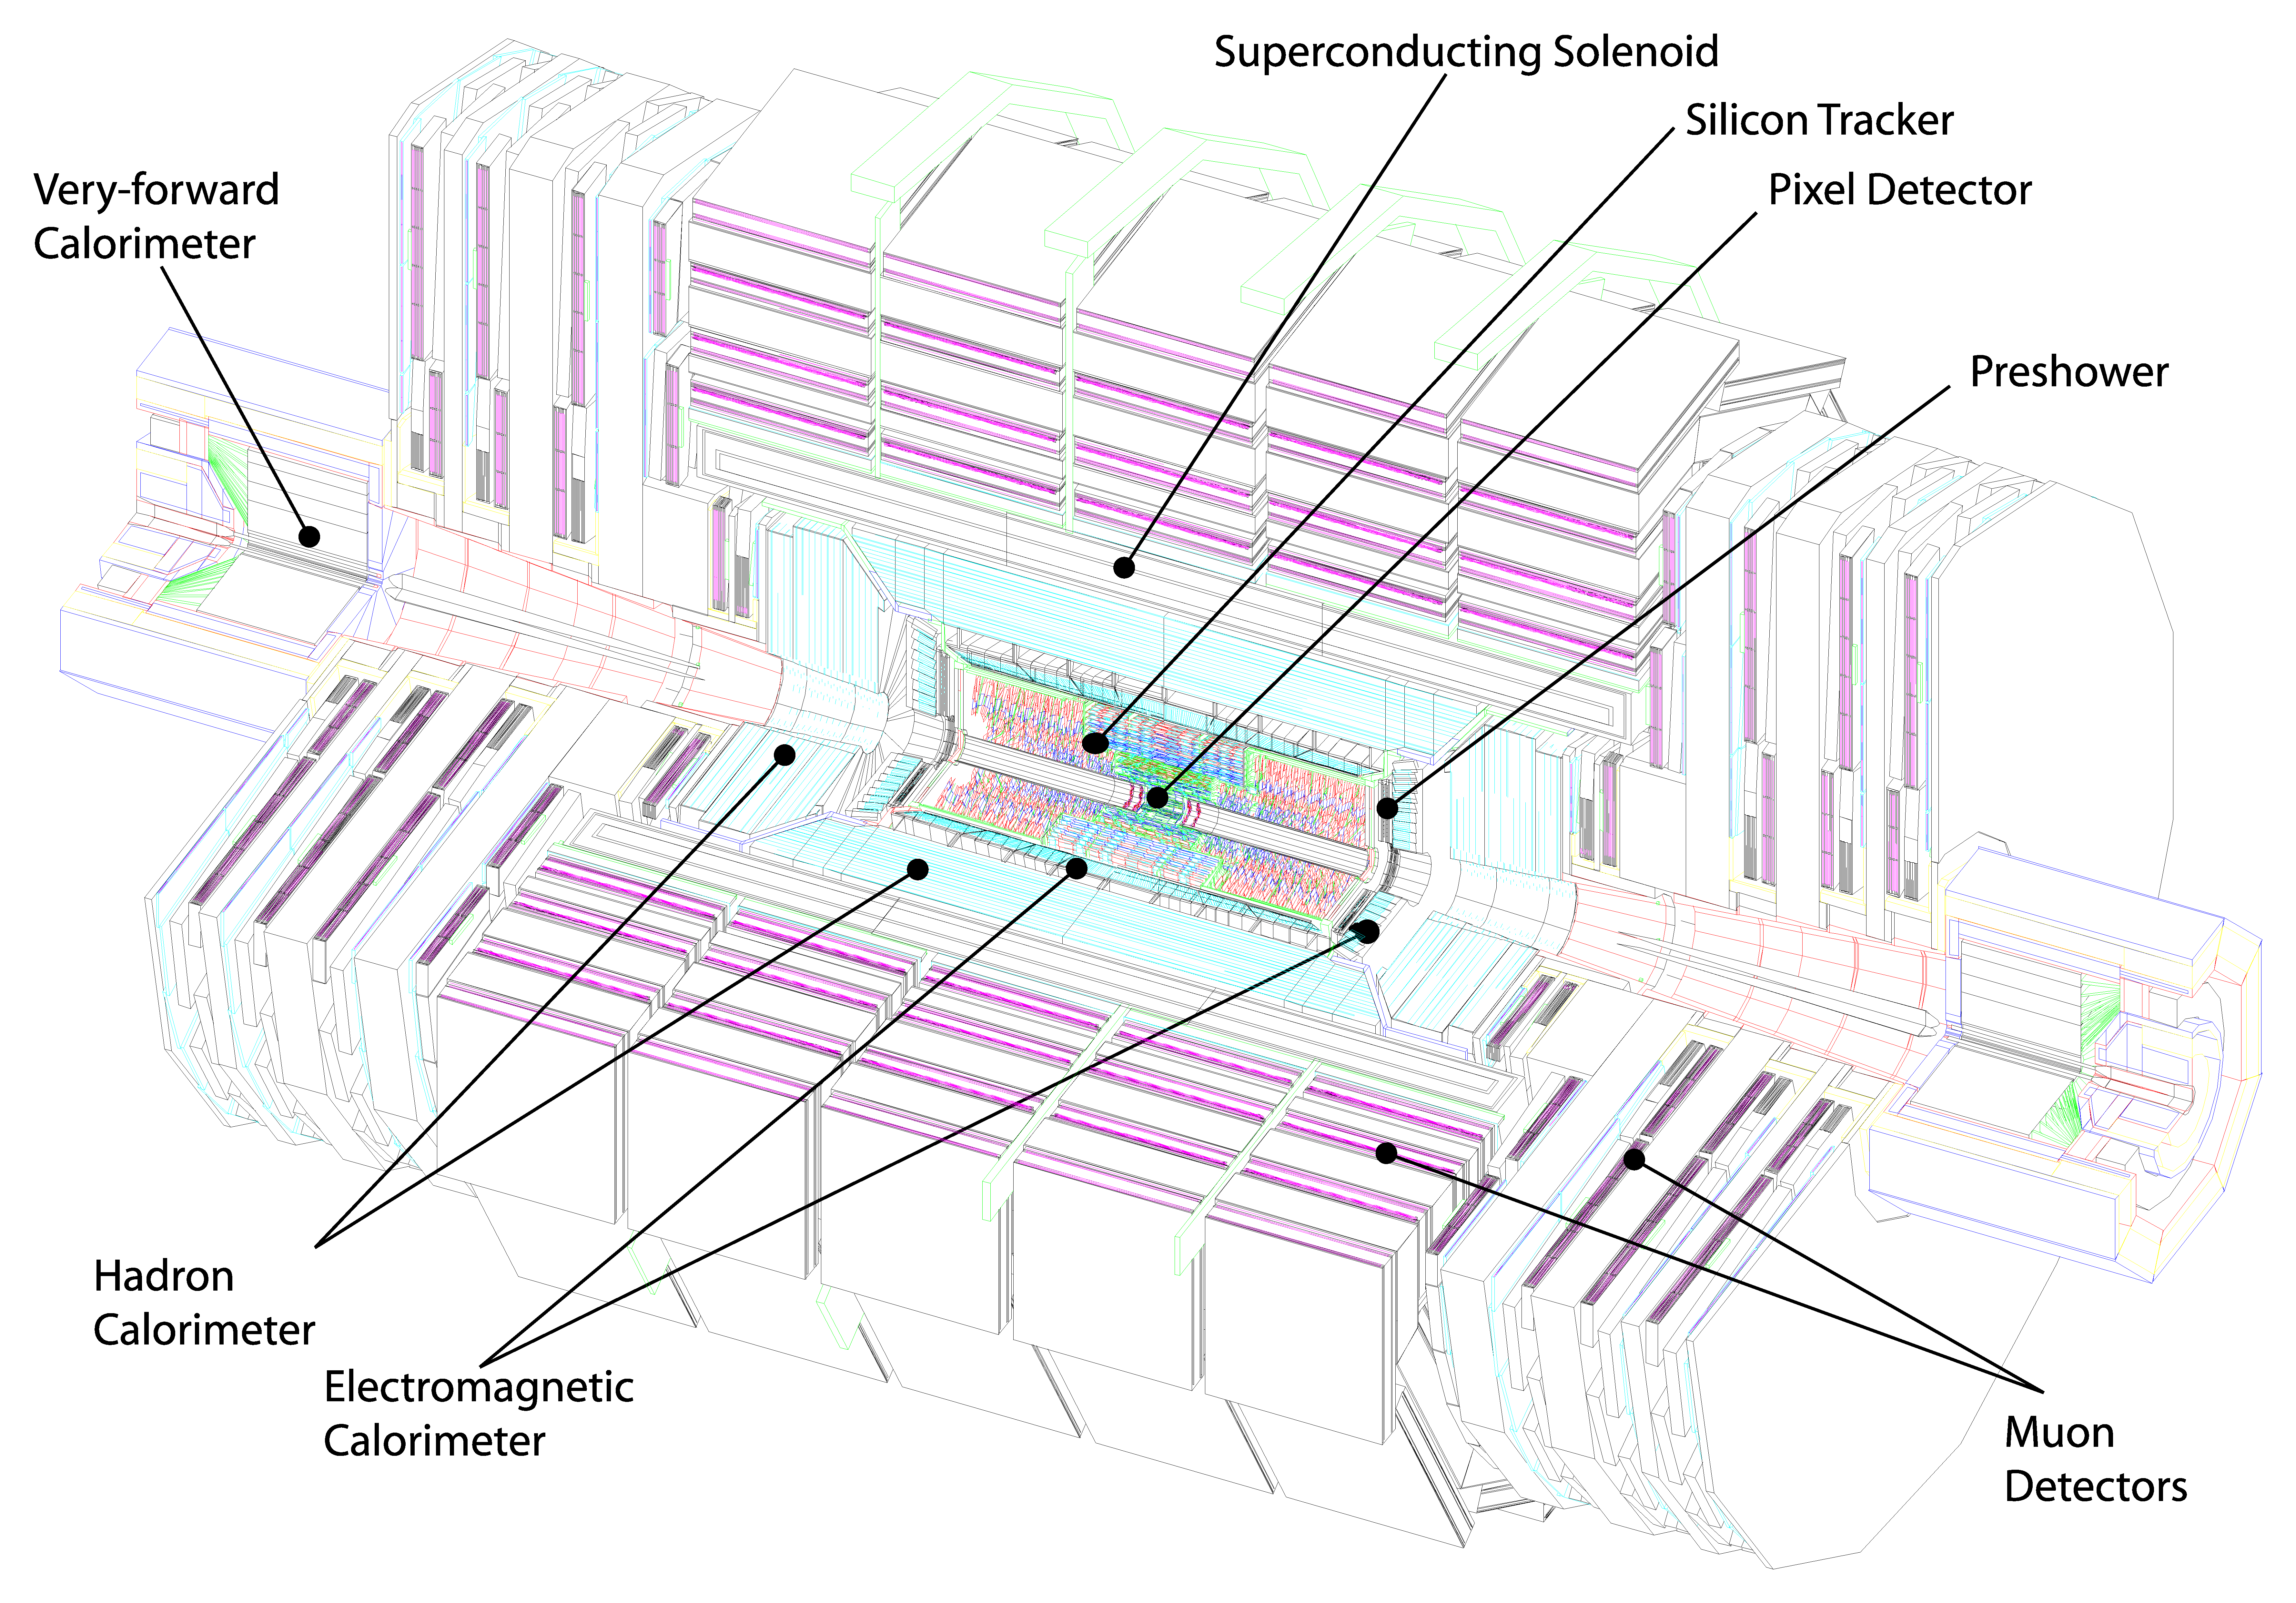
\includegraphics[width=0.7\textwidth]{chapitre2/figs/CMS_2.pdf}
  \caption{Vue en perspective du détecteur CMS}
  \label{fig:cms}
\end{figure}

Les travaux effectués dans cette thèse ayant tous été réalisés à l'aide des données collectées par le détecteur CMS, il est intéressant d'étudier plus en détails sa composition.

\bigskip

CMS (figure \ref{fig:cms}) est situé au point 5 du LHC. C'est un détecteur relativement compact, mesurant \SI{28.7}{\m} de long avec un rayon de \SI{7.5}{\m}, pour un poids de \SI{14000}{\tonne}. Afin de pouvoir définir correctement certaines variables, il est nécessaire de définir un repère. L'origine de ce repère se situe au centre du détecteur. L'axe $x$ pointe vers le centre de l'anneau du LHC, et l'axe $z$ est tangent à la direction du faisceau. L'axe $y$, perpendiculaire aux deux autres axes, pointe vers le haut.

L'angle azimutal $\phi \in \left[-\pi, \pi\right]$ est mesuré dans le plan $yx$, à partir de l'axe $x$. L'angle $\theta$, lui, est défini à partir de l'axe $z$ dans le plan transverse $yz$. On préfère cependant utilisé la pseudo-rapidité $\eta$ plutôt que $\theta$, puisque la production de particules est constante suivant $\eta$, mais pas suivant $\theta$. On défini la pseudo-rapidité par
\begin{align*}
  \eta &= -\ln\left[\tan\left(\frac{\theta}{2}\right)\right] = \frac{1}{2} \ln\left(\frac{\abs{\vec{p}} + p_L}{\abs{\vec{p}} - p_L}\right)
\end{align*}
où $p_L$ est la projection de l'impulsion le long de l'axe du faisceau.

Le LHC étant un collisionneur hadronique, il n'est pas possible de connaître à l'avance l'énergie exacte de la collision. En effet, les hadrons n'étant pas des particules élémentaires, ce sont les partons qui vont interagir, chacun emportant de façon aléatoire une fraction de l'impulsion disponible. On peut cependant appliquer la conservation de l'énergie dans le plan transverse, puisque, comme le faisceau se déplace uniquement le long de l'axe $z$, le bilan d'énergie dans le plan transverse $xy$ doit être nul. Il est alors commode de définir différentes variables transverses, telle que l'impulsion transverse ou l'énergie transverse, définies comme la projection vectorielle dans le plan $xy$. On a ainsi
\begin{align*}
  \pt &= \sqrt{p_x^2 + p_y^2} = \frac{\abs{\vec{p}}}{\cosh\eta} \\
  \et &= E \sin\theta = \frac{E}{\cosh\eta}
\end{align*}

%Pour un détecteur parfait ayant une couverture angulaire totale, on doit avoir $\et = 0$.

L'un des objectifs principaux de CMS, qui figure d'ailleurs dans son nom, est de pouvoir mesurer avec une grande précision l'impulsion des particules, même celles les plus boostées, et particulièrement l'impulsion des muons. On utilise pour cela un champ magnétique intense de \SI{3.8}{\tesla}, produit grâce à un solénoïde, afin de courber la trajectoire des particules. CMS est aussi constitué de couches de de sous-détecteurs, apportant chacun des informations particulières sur la collision, telles que l'énergie des particules, leurs trajectoires mais aussi leur identité. Chaque sous-détecteur est décrit en détail dans les sections suivantes.

\begin{figure}[t] \centering
  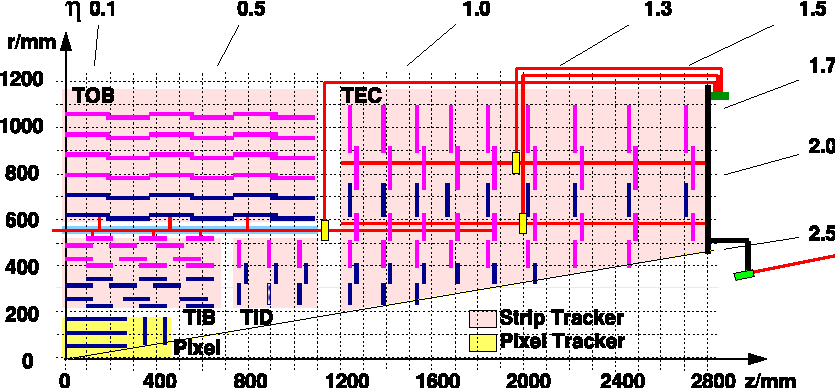
\includegraphics[width=0.7\textwidth]{chapitre2/figs/tracker.pdf}
  \caption{Représentation simplifiée du trajectographe de l'expérience CMS.}
  \label{fig:tracker}
\end{figure}

\subsection{Le trajectographe}

Le trajectographe est l'un des composants les plus important de CMS. Il est en effet chargé de reconstruire la trajectoire courbée des particules chargées, et ainsi d'en déduire leur impulsion, mais aussi de reconstruire les vertex d'interactions. Cylindre d'une longueur de \SI{5.5}{\m} et de \SI{1.1}{\m} de rayon, le trajectographe est composée de deux parties, conçues pour couvrir une région angulaire entre $0 < \eta < \num{2.5}$.

\smallskip

La première partie est le détecteur à pixels. Il est composé de trois couches de détections situées au plus proche du point de collision (à $r = \SI{4}{\cm}$, $r = \SI{7}{\cm}$ et $r = \SI{11}{cm}$), et de quatre disques (bouchons) disposés 2 à 2 à chaque extrémité ($z = \pm \SI{34.5}{\cm}$ et $z = \pm \SI{46.5}{\cm}$). Ce détecteur en silicium comporte environ 65 millions de pixels, mesurant chacun \SI{100}{\um} par \SI{150}{\um}, pour une superficie totale de détection d'environ \SI{1}{\square\m}. Sa résolution est inférieure à $\SI{10}{\um}$ dans le plan $r\phi$ (voir figure \ref{fig:pixel_resolution}) et $\SI{20}{\um}$ en $Z$.

La deuxième partie est le détecteur à micropistes. Englobant le détecteur à pixels, ce détecteur est composé de plus de 10 couches en silicium, pour un total d'environ 10 millions de micropistes. On dénombre 4 sous-ensemble :

\begin{description}
  \item[Le TIB] (\emph{Tracker Inner Barrel}) C'est la partie interne du tonneau du trajectographe, composée de 4 couches de micropistes.
  \item[Le TID] (\emph{Tracker Inner enDcaps}) Cette partie constitue les bouchons internes, et complète le TIB. Elle compte trois couches de détection.
  \item[Le TOB] (\emph{Tracker Outer Barrel}) Entourant le TIB, cette partie du tonneau externe est constituée de six couches de micropistes.
  \item[Le TEC] (\emph{Tracker EndCaps}) Composée de neuf couches, cette partie complète le TOB. Elle forme les deux bouchons externes.
\end{description}

L'agencement du trajectographe, avec les détecteurs à pixels et à micropistes, est présenté en détails figure \ref{fig:tracker}.

\begin{figure} \centering
  \subcaptionbox{Évolution de la résolution dans le plan $r\phi$ du détecteur à pixel du trajectographe en fonction de la luminosité totale collectée, déterminée à l'aide des données collectées en 2012.\label{fig:pixel_resolution}}[.45\textwidth]{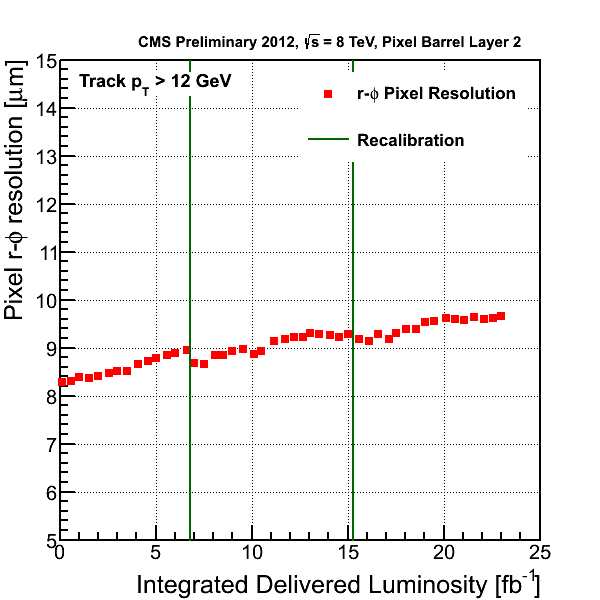
\includegraphics[width=0.45\textwidth]{chapitre2/figs/pixel_detector_resolution_over_time.png}}\hfill
  \subcaptionbox{Efficacité de reconstruction des coups du détecteur à pixel du trajectographe en fonction de la luminosité instantanée, déterminée à l'aide des données collectées en 2012.\label{fig:pixel_efficiency}}[.45\textwidth]{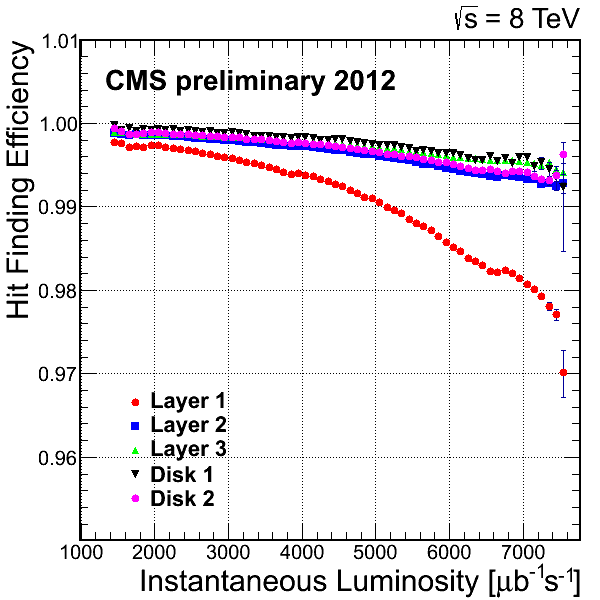
\includegraphics[width=0.45\textwidth]{chapitre2/figs/pixel_detector_efficiency_over_time.png}}
  \caption{Résolution (\subref{fig:pixel_resolution}) et efficacité de reconstruction (\subref{fig:pixel_efficiency}) du détecteur à pixels du trajectographe.}
\end{figure}

\subsection{Le calorimètre électromagnétique}

Situé juste après le trajectographe, le calorimètre électromagnétique (ECAL) sert à mesurer de façon précise l'énergie des électrons et des photons. Sachant qu'un des canaux majeurs d'étude du boson de Higgs est sa désintégration en deux photons, un soin tout particulier a été apporté lors de la conception de ce calorimètre.

Une des contraintes majeures qui a dicté sa conception est l'espace disponible entre le trajectographe et le solénoïde, assez réduit. Ce manque de place a éliminé la technologie la plus avancée existante à l'époque de la conception, le calorimètre à argon liquide\footnote{C'est la technologie qu'a choisi ATLAS pour son calorimètre électromagnétique.}. Il a au final été choisi d'utiliser un détecteur à scintillation, formé d'un ensemble de cristaux de tungstate de plomb ($PbWO_4$). Le calorimètre couvre une région angulaire entre $0 < \abs{\eta} < 3$, et est séparé en deux parties : le tonneau (EB, pour \emph{ECAL Barrel}, $0 < \abs{\eta} < \num{1.479})$ et le bouchon (EE, pour \emph{ECAL Endcap}, $\num{1.479} < \abs{\eta} < 3$).

\subsubsection{Les cristaux}

Le ECAL est constitué de 76200 cristaux de tungstate de plomb : 61200 dans le tonneau, et 15000 dans les bouchons. Le choix du tungstate de plomb a été dicté par plusieurs contraintes : la résistance aux radiations, le coût, mais principalement un encombrement réduit. En effet, ses cristaux ont été spécialement conçu pour avoir une faible longueur de radiation\footnote{Longueur pour qu'un électron perde $\sfrac{2}{3}$ de son énergie.} ($X_0 = \SI{0.89}{\cm}$), ce qui permet d'utiliser des cristaux ayant une épaisseur modeste ($\num{25.8}X_0$ dans le tonneau, et $\num{24.7}X_0$ dans les bouchons) tout en stoppant les particules même les plus énergétiques. Un autre aspect très intéressant du $PbWO_4$ est son faible rayon de molière (\SI{2.19}{\cm}) \footnote{90\% de l'énergie de la gerbe électromagnétique est contenue dans un cylindre de rayon le rayon de molière.}. Il est ainsi possible d'utiliser des cristaux ayant des dimensions très réduites (\SI{21.8}{\mm} $\times$ \SI{21.8}{\mm} dans le tonneau, et \SI{24.7}{\mm} $\times$ \SI{24.7}{\mm} dans les bouchons), ce qui permet d'obtenir une très grande granularité en $\eta$ et $\phi$.
En contrepartie de ces excellentes caractéristiques, les cristaux de tungstate de plomb ont un inconvénient majeur : leur réponse est très sensible à la température (\tilde $\SI[per-mode = symbol]{2}{\percent\per\degreeCelsius}$). Il est donc nécessaire de maintenir une température très stable dans ECAL : un système de refroidissement permet de maintenir la température dans le ECAL à $\pm \SI{0.05}{\degreeCelsius}$.

\medskip

Le calorimètre électromagnétique est un détecteur à scintillation : lors du passage d'un électron ou d'un photon, de la lumière est émise en quantité proportionnelle à l'énergie déposée dans le cristal. Afin de collecter cette lumière, des photodétecteurs sont associés à chaque cristal. Les conditions de fonctionnement dans le détecteur étant rude (champ magnétique de \SI{8.3}{\tesla}, très fortes radiations), deux technologies différentes ont été retenues : les photodiodes à avalanches pour le tonneau (APD), et les phototriodes à vide pour les bouchons (VPT).

\subsubsection{Le détecteur à pied de gerbe}

On a vu qu'un des canaux de détection le plus prometteur pour le boson de Higgs est sa désintégration en deux photons. Cependant, certains hadrons neutres, tels que les $\pi^0$, peuvent imiter la présence d'un photon énergique lorsqu'ils se désintègrent en deux photons. Ces deux photons sont très proche l'un de l'autre, et la granularité du calorimètre n'est pas suffisante pour les détecter comme deux particules distinctes. A la place, un unique photon énergétique sera détecté. Afin de palier à ce problème, il a été décidé de placer un détecteur à pied de gerbe juste avant le calorimètre électromagnétique, uniquement dans les bouchons\footnote{Un détecteur à pied de gerbe est aussi prévu pour le tonneau, mais n'est pas encore installé}. Ce détecteur, couvrant une région en $\abs{\eta}$ entre \num{1.653} et \num{2.6}, permet d'initier la gerbe électromagnétique avant d'entrer dans le ECAL, grâce à une plaque de plomb et d'aluminium. Composé d'une surface de détection en silicium de \SI{8}{\square\meter}, il possède une granularité bien plus importante que le ECAL, avec des bandes de détection de \SI{2}{\mm} de large. Il est ainsi possible de distinguer correctement les photons issus d'un $\pi^0$ boosté.

\begin{figure}[t] \centering
  \subcaptionbox{Réponse relative des cristaux en fonction du temps, pour différentes zones en \aeta. \label{fig:ecal_transparency}}[0.45\textwidth]{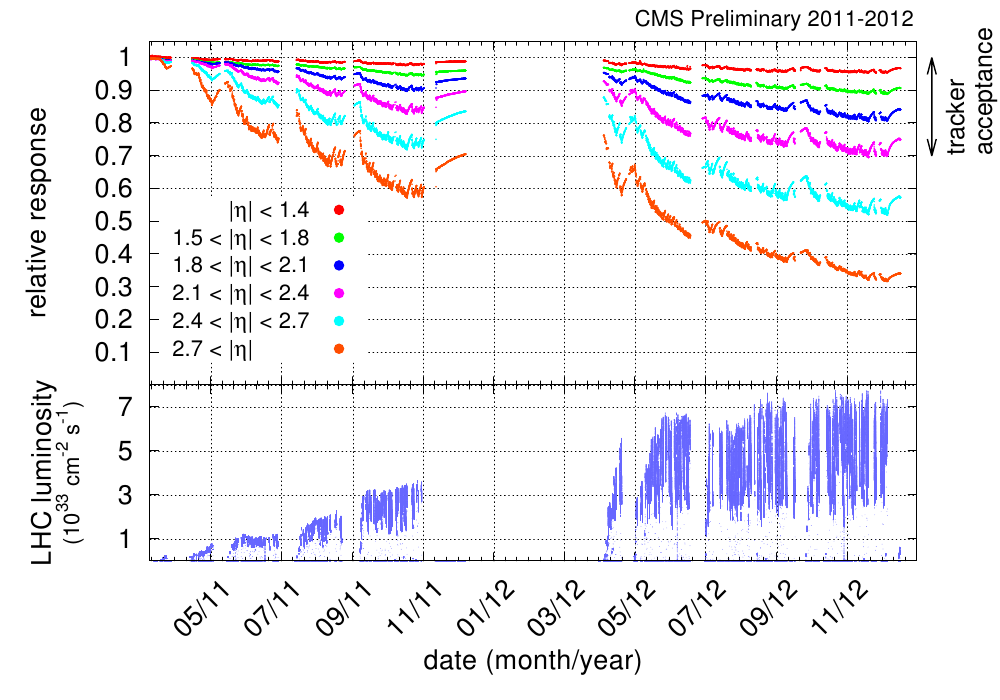
\includegraphics[width=0.45\textwidth]{chapitre2/figs/ecal_transparency.png}} \hfill
  %\subcaptionbox{Résolution relative en énergie des cristaux en fonction de $\eta$ des superclusters.}[0.45\textwidth]{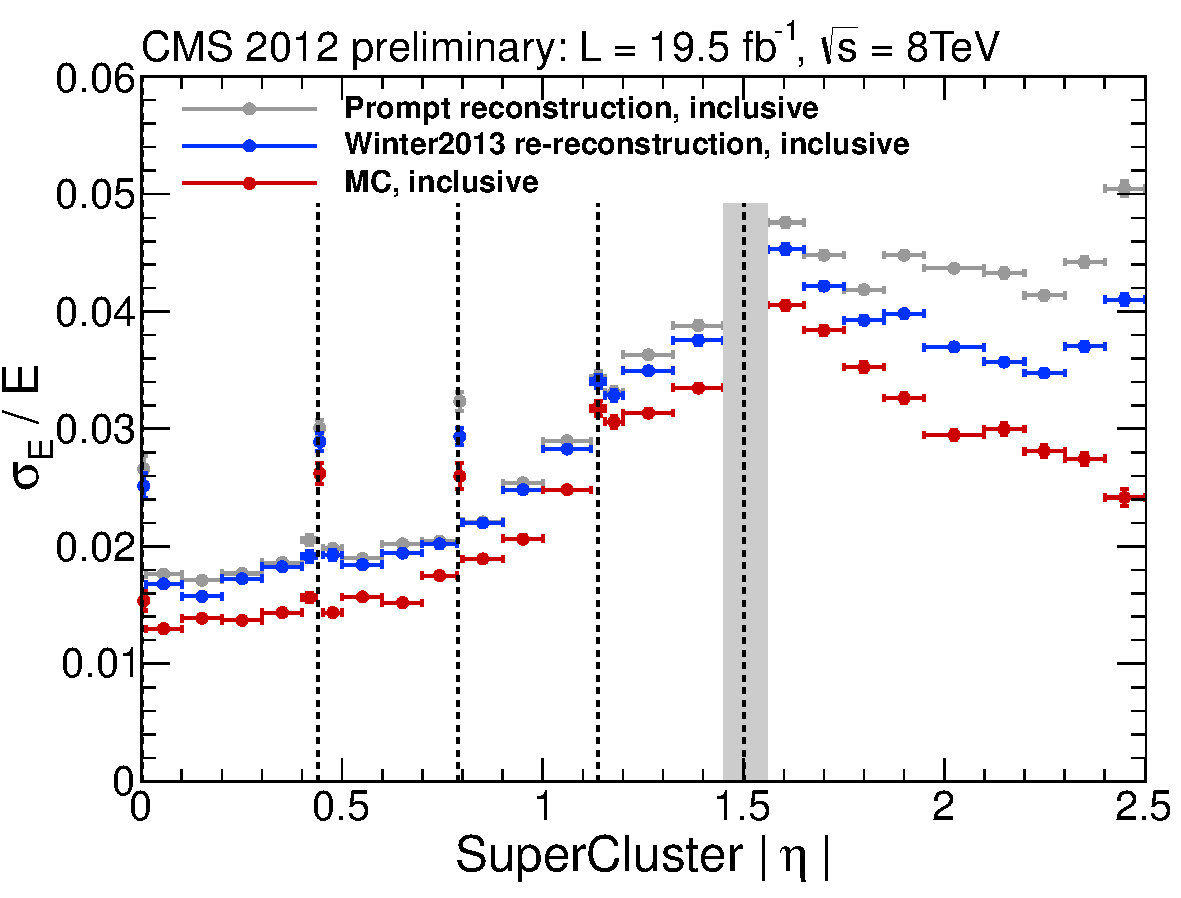
\includegraphics[width=0.45\textwidth]{chapitre2/figs/ecal_resolution.pdf}}
  \subcaptionbox{Effet des corrections de transparence des cristaux sur la masse invariante $M_{ee}$ sur des événements $Z \rightarrow ee$. \label{fig:ecal_corrections}}[0.45\textwidth]{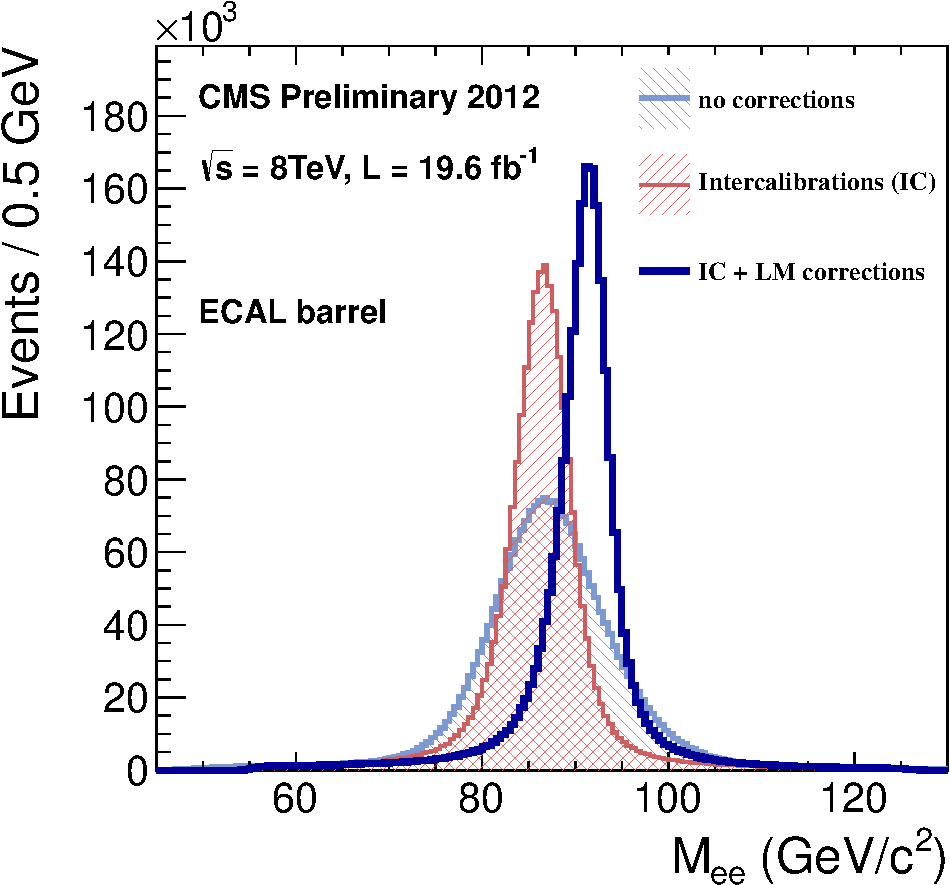
\includegraphics[width=0.45\textwidth]{chapitre2/figs/ecal_corrections_effect.pdf}}
  \caption{Performance des cristaux du ECAL}
  \label{fig:ecal_performance}
\end{figure}

\subsubsection{Performances}

Les cristaux du ECAL sont très sensibles aux radiations, et perdent de la transparence au fil du temps. Afin de mesurer cet effet, un système de contrôle a été mis en place. Toutes les 20 minutes, un laser est envoyé dans tous les cristaux afin de mesurer leur transparence. On peut voir figure \ref{fig:ecal_transparency} la réponse relative des cristaux du ECAL en fonction de la date de prise de données. On voit clairement la diminution de la réponse, due à l'impact des radiations sur les cristaux. Des corrections sont déployées après coup pour corriger cet effet. On peut voir figure \ref{fig:ecal_corrections} l'effet de ces corrections. La courbe hachurée bleue représente le spectre de masse invariante des événements $\PZ \rightarrow \Pelectron \APelectron$ sans aucune correction. En ajoutant graduellement les corrections de transparence du ECAL, on obtient la courbe rouge, puis la courbe bleue. On voit une très nette amélioration de la valeur moyenne et de la résolution.

\bigskip

La résolution du ECAL peut être paramétrée de la façon suivante :
\begin{align*}
  \left( \frac{\sigma}{E} \right)^2 &= \left( \frac{S}{\sqrt{E}} \right)^2 + \left( \frac{N}{E} \right)^2 + C^2
\end{align*}
où $S$ est le terme stochastique, dû aux fluctuations dans l'étalement latéral de la gerbe électronique, $N$ le terme de bruit, dû aux bruits des composants électroniques, et $C$ le terme constant, dû principalement aux erreurs d'inter-calibrations.

Elle a été évaluée lors de tests sur faisceaux en 2006 à
\begin{align*}
  \left( \frac{\sigma}{E} \right)^2 &= \left( \frac{\SI{2.8}{\%}}{\sqrt{E}} \right)^2 + \left( \frac{\num{0.12}}{E} \right)^2 + \left(\SI{0.30}{\%}\right)^2
\end{align*}
ce qui équivaut, pour un électron de $E = \SI{120}{\GeV}$, à $\sigma = \SI{1.90}{\GeV}$. Récemment, la résolution du ECAL a été évaluée en utilisant les données collectées en 2012. On peut voir figure \ref{fig:ecal_resolution} l'évolution de la résolution en fonction de la position angulaire des super-clusters. On constate que pour $\abs{\eta} < 1.3$, la résolution est inférieure à \SI{3}{\%}, soit $\sigma = \SI{3.6}{\GeV}$. C'est donc une excellente performance pour le détecteur.

\begin{figure} \centering
  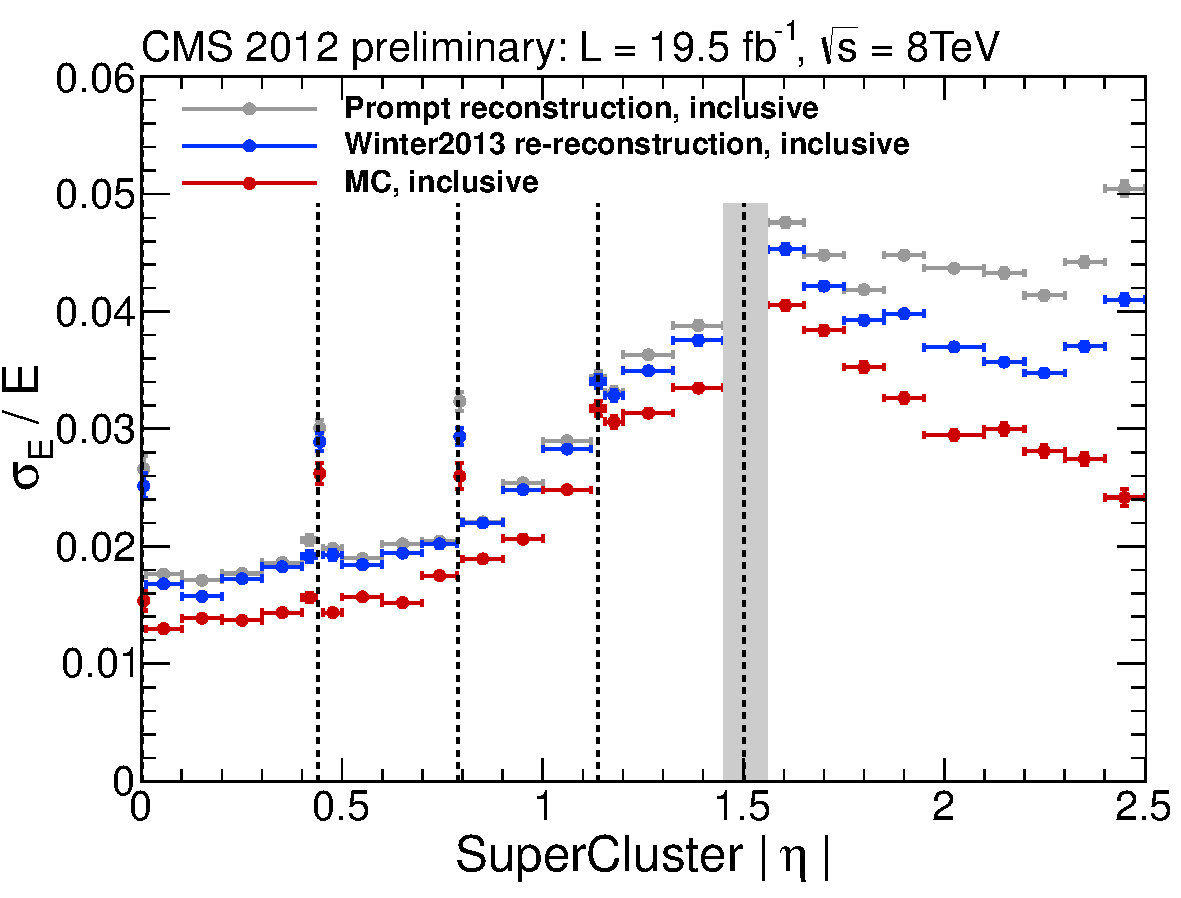
\includegraphics[width=0.4\textwidth]{chapitre2/figs/ecal_resolution.pdf}
  \caption{Évolution de la résolution totale du ECAL en fonction de la position angulaire $\eta$ du super-cluster}
  \label{fig:ecal_resolution}
\end{figure}

\subsection{Le calorimètre hadronique} \label{sec:hcal}

Le rôle du calorimètre hadronique (HCAL, pour \emph{Hadronic CALorimeter}) est de mesurer l'énergie des hadrons neutres et chargés, grâce à l'utilisation d'un détecteur à échantillonnages. Une succession de couches d'absorbants et de scintillateurs permettent de déterminer la trajectoire et l'énergie d'une particule incidente. De façon analogue au calorimètre électromagnétique, il est constitué de deux parties : une partie tonneau et deux bouchons.

L'absorbant retenu pour le tonneau et les bouchons est le laiton. Étant installé au sein d'un puissant champ magnétique, il fallait en effet choisir un métal paramagnétique. Le laiton a aussi l'avantage d'être quasi transparent pour les muons : leur détection intervenant après le HCAL, il est en effet important que les muons ne perdent pas d'énergie dans le HCAL, au risque de biaiser l'estimation de leur impulsion. Chaque couche d'absorbant mesure \SI{5}{\cm} d'épaisseur dans le tonneau, et \SI{8}{\cm} dans les bouchons. Entre chaque couche d'absorbant se trouve une couche de scintillateur plastique de \SI{3.7}{\mm} d'épaisseur. La lumière produite lors du passage d'une particule est collectée par des fibres optiques, puis amplifiée par des photodiodes hybrides.

\medskip

Le tonneau couvre une zone angulaire entre $0 \leq \abs{\eta} < \num{1.48}$, et est composé de deux parties différentes. La première partie, le HB, mesure \SI{89}{\cm} de profondeur, soit seulement \SI{5.82}{\lambda_0}\footnote{La longueur d'interaction nucléaire, $\lambda_0$, est une longueur caractéristique des matériaux. C'est la longueur après laquelle \SI{36.8}{\%} ($\sfrac{1}{e}$) des hadrons sont absorbés par le milieu. Pour le laiton, on a $\lambda_0 = \SI{16.42}{\cm}$}. Cette longueur est insuffisante pour absorber la totalité de la gerbe hadronique. Une deuxième partie, le HO, a donc été ajouté, située à l'extérieur du solénoïde. L'aimant sert alors d'absorbeur, et le HO détecte les gerbes longues ou tardives. Les bouchons couvrent eux une zone angulaire entre $1.48 \leq \abs{\eta} < \num{3}$. La longueur totale du calorimètre est, en incluant le ECAL, d'environ \SI{10}{\lambda_0}, suffisant pour stopper la gerbe hadronique.

\bigskip

Ainsi constitué, le HCAL couvre une région angulaire entre $0 \leq \abs{\eta} < \num{3}$. Cependant, afin de correctement mesurer l'énergie manquante dans la collision, il est important de couvrir au maximum tout l'espace angulaire. Ainsi, un détecteur parfait couvrirait une zone $0 \leq \abs{\eta} < \infty$. Ce n'est malheureusement pas possible puisqu'il faut laisser un espace libre pour le faisceau de particules. Le HCAL comprend une troisième partie, plus à l'avant, couvrant une zone angulaire entre $\num{3} \leq \abs{\eta} < \num{5}$, le HF. C'est un cylindre de \SI{130}{\cm} de rayon, situé à \SI{11.2}{\m} du point d'interaction. D'une longueur de \SI{165}{\cm} (\tilde \SI{10}{\lambda_0}), il est constitué d'un absorbeur en acier, dans lequel sont introduites des fibres optiques en quartz. Les particules chargées entrant dans le milieu émettent de la lumière Cherenkov, collectée par les fibres puis amplifiée. Ce détecteur est ainsi principalement sensible à la partie électromagnétique des gerbes hadroniques.

\fxerror{Mettre quelques lignes sur la mesure de la luminosité dans le HF ?}

\subsection{Le solénoïde}

L'aimant supraconducteur de CMS a été conçu afin de fournir un champ magnétique de \SI{3.8}{\tesla}. De forme cylindrique de rayon \SI{6}{\m}, long de \SI{12.5}{\meter}, il est parcouru par un courant électrique de \SI{19.14}{\kilo\ampere}. Afin de maintenir son état supraconducteur, l'aimant est refroidi par un système de cryostat fonctionnant à l'hélium superfluide. Il est ainsi constamment maintenu à une température de \SI{1.9}{\kelvin}.

On a vu déjà précédemment l'intérêt d'un puissant champ magnétique. En effet, la trajectoire d'une particule chargée se courbe en présence d'un champ magnétique, avec un rayon de courbure proportionnel à son impulsion :
\begin{align*}
  r &= \frac{p}{qB}
\end{align*}
avec $r$ le rayon de courbure de la trajectoire, $p$ l'impulsion, $q$ la charge de particule et $B$ l'intensité du champ magnétique. Plus $r$ est petit, plus il est simple à mesurer, puisque la courbure de la trajectoire est plus prononcée. Afin de mesurer de façon précise l'impulsion des particules, même les plus boostées, il est donc nécessaire d'utiliser un champ magnétique puissant afin d'optimiser $r$.

\subsection{Le détecteur à muons}

\begin{figure}[tb] \centering
  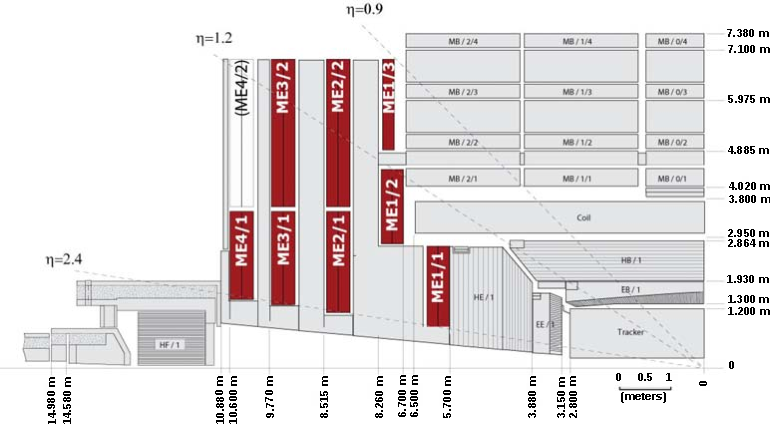
\includegraphics[width=0.8\textwidth]{chapitre2/figs/CSC.pdf}
  \caption{Vue un-quart du détecteur CMS. Les chambres à pistes cathodiques des bouchons sont illustrées en rouge.}
  \label{fig:cms_csc}
\end{figure}


Le détecteur à muons joue un rôle central dans CMS, puisqu'il couvre trois fonctions principales : identifier les muons, mesurer leur impulsion, et assurer une partie du déclenchement. C'est la partie la plus externe de CMS, que seul les muons peuvent atteindre. Il est ainsi beaucoup plus facile de mesurer l'impulsion de ces particules, grâce à l'éloignement entre le trajectographe et ce détecteur.

\begin{figure}[p] \centering
  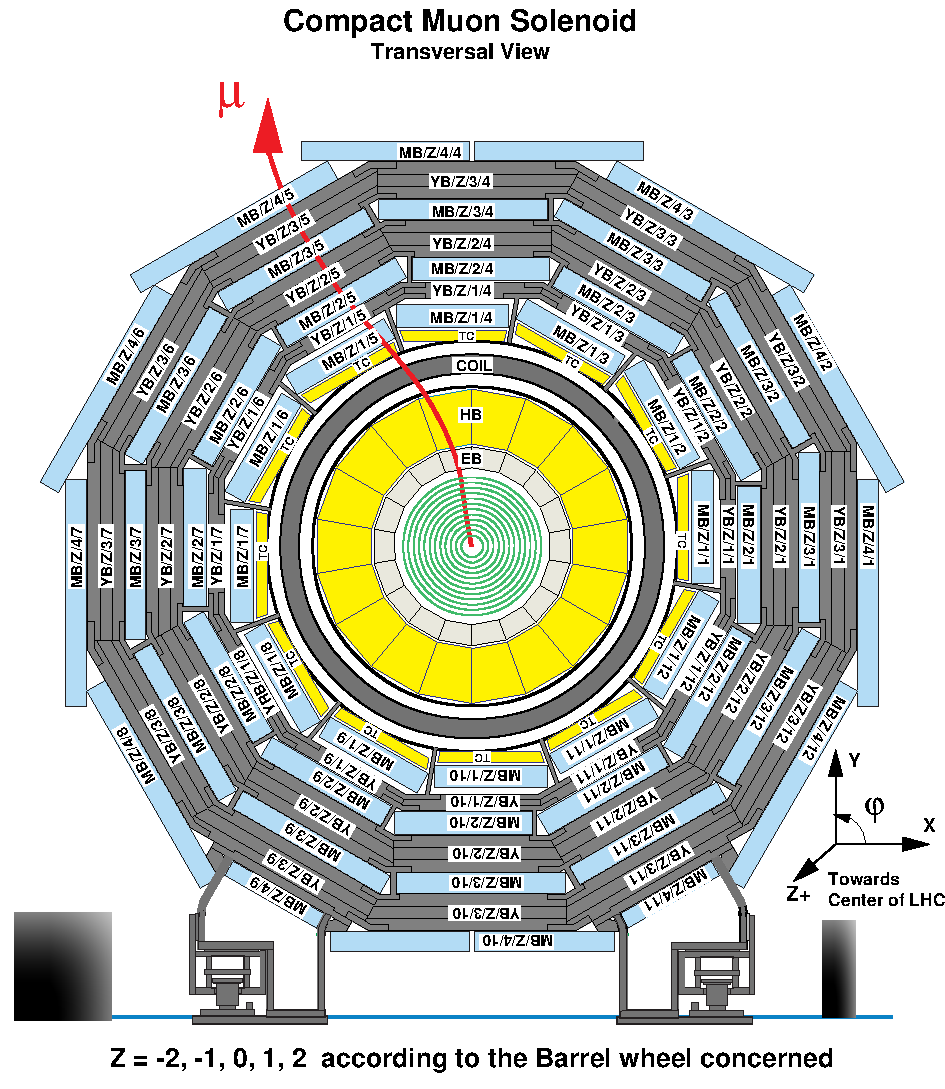
\includegraphics[width=0.95\textwidth]{chapitre2/figs/CMS_transverse_view.pdf}
  \caption{Agencement des tubes à dérives dans le tonneau de CMS (vue transverse). Chaque rectangle bleu correspond à un tube à dérive.}
  \label{fig:cms_dt}
\end{figure}

On trouve trois technologies différentes au sein du détecteur à muons : les tubes à dérive (DT, pour \emph{Drift Tube}) et les chambres à pistes cathodique (CSC, pour \emph{Cathod Strip Chamber}), utilisés pour mesurer les propriétés des muons, et les détecteurs à plaques résistives (RPC, pour \emph{Resistive Plate Chamber}) utilisés par le système de déclenchement.

\begin{description}
  \item[Les tubes à dérive] Installés dans le tonneau (voir figure \ref{fig:cms_dt}), ces détecteurs couvrent une zone angulaire $\abs{\eta} < 1.2$. On en compte 250 dans le détecteur.
  \item[Les chambres à pistes cathodiques] Ces détecteurs sont utilisés dans les bouchons (voir figure \ref{fig:cms_csc}), là où le champ magnétique n'est pas constant et le taux de radiation élevé. 540 de ces modules sont installés, couvrant une zone angulaire $\num{0.9} < \abs{\eta} < \num{2.4}$.
  \item[Les détecteurs à plaques résistives] Présents à la fois dans le tonneau et dans les bouchons, ils permettent d'assurer une partie du déclenchement. En effet, leur temps de réponse est bien inférieur à \SI{25}{\ns}, ce qui permet de décider très rapidement si un événement est digne d’intérêt ou s'il peut être jeté.
\end{description}

%\subsubsection{Performances}

\subsection{Le système de déclenchement}

\begin{figure} \centering
  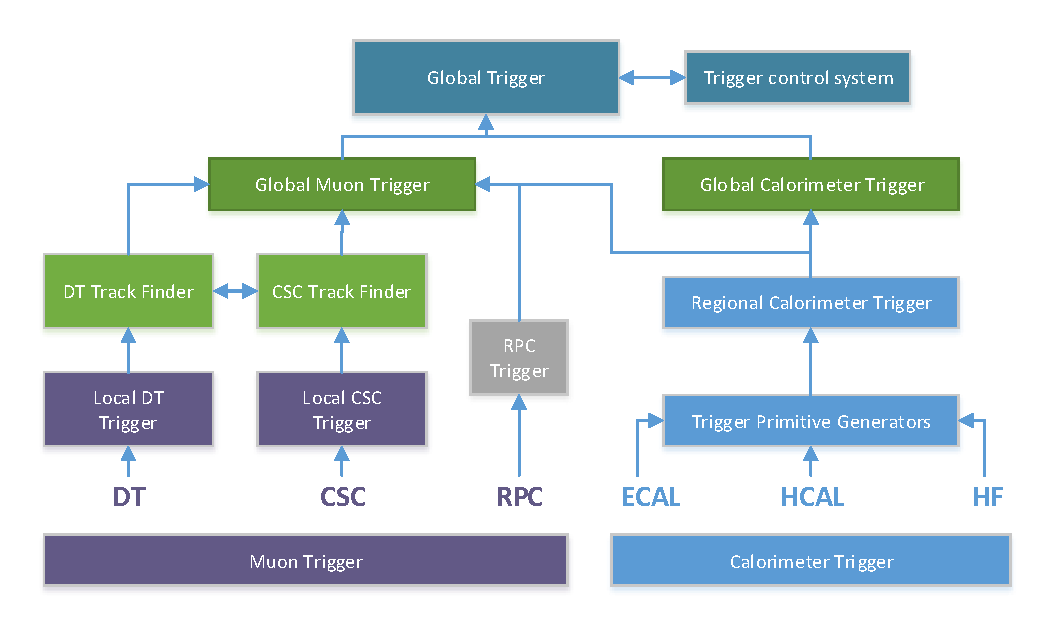
\includegraphics[width=0.7\textwidth]{chapitre2/figs/L1.pdf}
  \caption{L'architecture du déclencheur de niveau 1}
  \label{fig:l1}
\end{figure}

Aux conditions nominales, le temps entre chaque collision est de \SI{25}{\ns}, soit une fréquence de \SI{40}{\mega\hertz}. En estimant la taille d'un événement à environ \SI{1}{\mega\octet}, on obtient alors un débit de données de \SI{40}{\tera\octet\per\second}, débit bien trop élevé pour être traité en temps réel. Il est donc nécessaire de réduire ce débit en jetant des événements. Tout l'enjeu est de réussir à jeter des événements dont on sait à l'avance qu'ils ne seront pas intéressant (pas de collision de grande intensité, bruit trop important, \ldots). On utilise pour cela un système de déclenchement (\emph{trigger}), composé dans CMS de deux niveaux : le niveau 1 (L1, figure \ref{fig:l1}) et le HLT (\emph{High Level Trigger}, pour déclencheur de haut niveau, figure \ref{fig:daq}). Ces systèmes doivent être capable de décider en temps réel si un événement à un intérêt physique ou non.

\begin{description}
  \item[Le L1] Ce premier niveau de déclenchement réduit le taux d’événements à \SI{100}{\kHz}, à l'aide d'un système électronique ultra-rapide. En utilisant directement les informations provenant du détecteur à muons et des calorimètres, la décision de garder ou non l'événement est prise en moins de \SI{3.2}{\us}. Cette électronique est hautement configurable, et peut être reconfigurée à tout moment. Ainsi, 128 algorithmes de déclenchement tournent en parallèle, ce qui permet de fournir des lot de données adaptées aux besoins des analyses de physique.
  \item[Le HLT] Le taux d'événements en sortie du L1 est encore trop important, et doit être réduit à environ \SI{400}{\Hz} afin d'être stockable en temps réel. Le HLT est chargée d'effectuée cette sélection. Pour cela, une ferme d'ordinateurs est installée à proximité du détecteur et sélectionne les événements digne d’intérêt. Il dispose des données de tous les sous-détecteurs et effectue une reconstruction rapide afin d'obtenir une description de l'événement en terme d'objets physiques plutôt qu'en terme de signaux électriques. Le temps moyen alloué au HLT pour prendre une décision est d'environ \SI{50}{\ms}. Les analyses de physique ayant des besoins particuliers, plusieurs chemins de déclenchement tournent en parallèle. On définit ainsi plusieurs lots de données, chacun regroupant une collection de chemins de déclenchement. On trouve par exemple le lot de données \emph{SingleMu}, qui regroupe les chemins de déclenchement demandant au moins un muon d'une certaine impulsion.
\end{description}

\begin{figure}[tb] \centering
  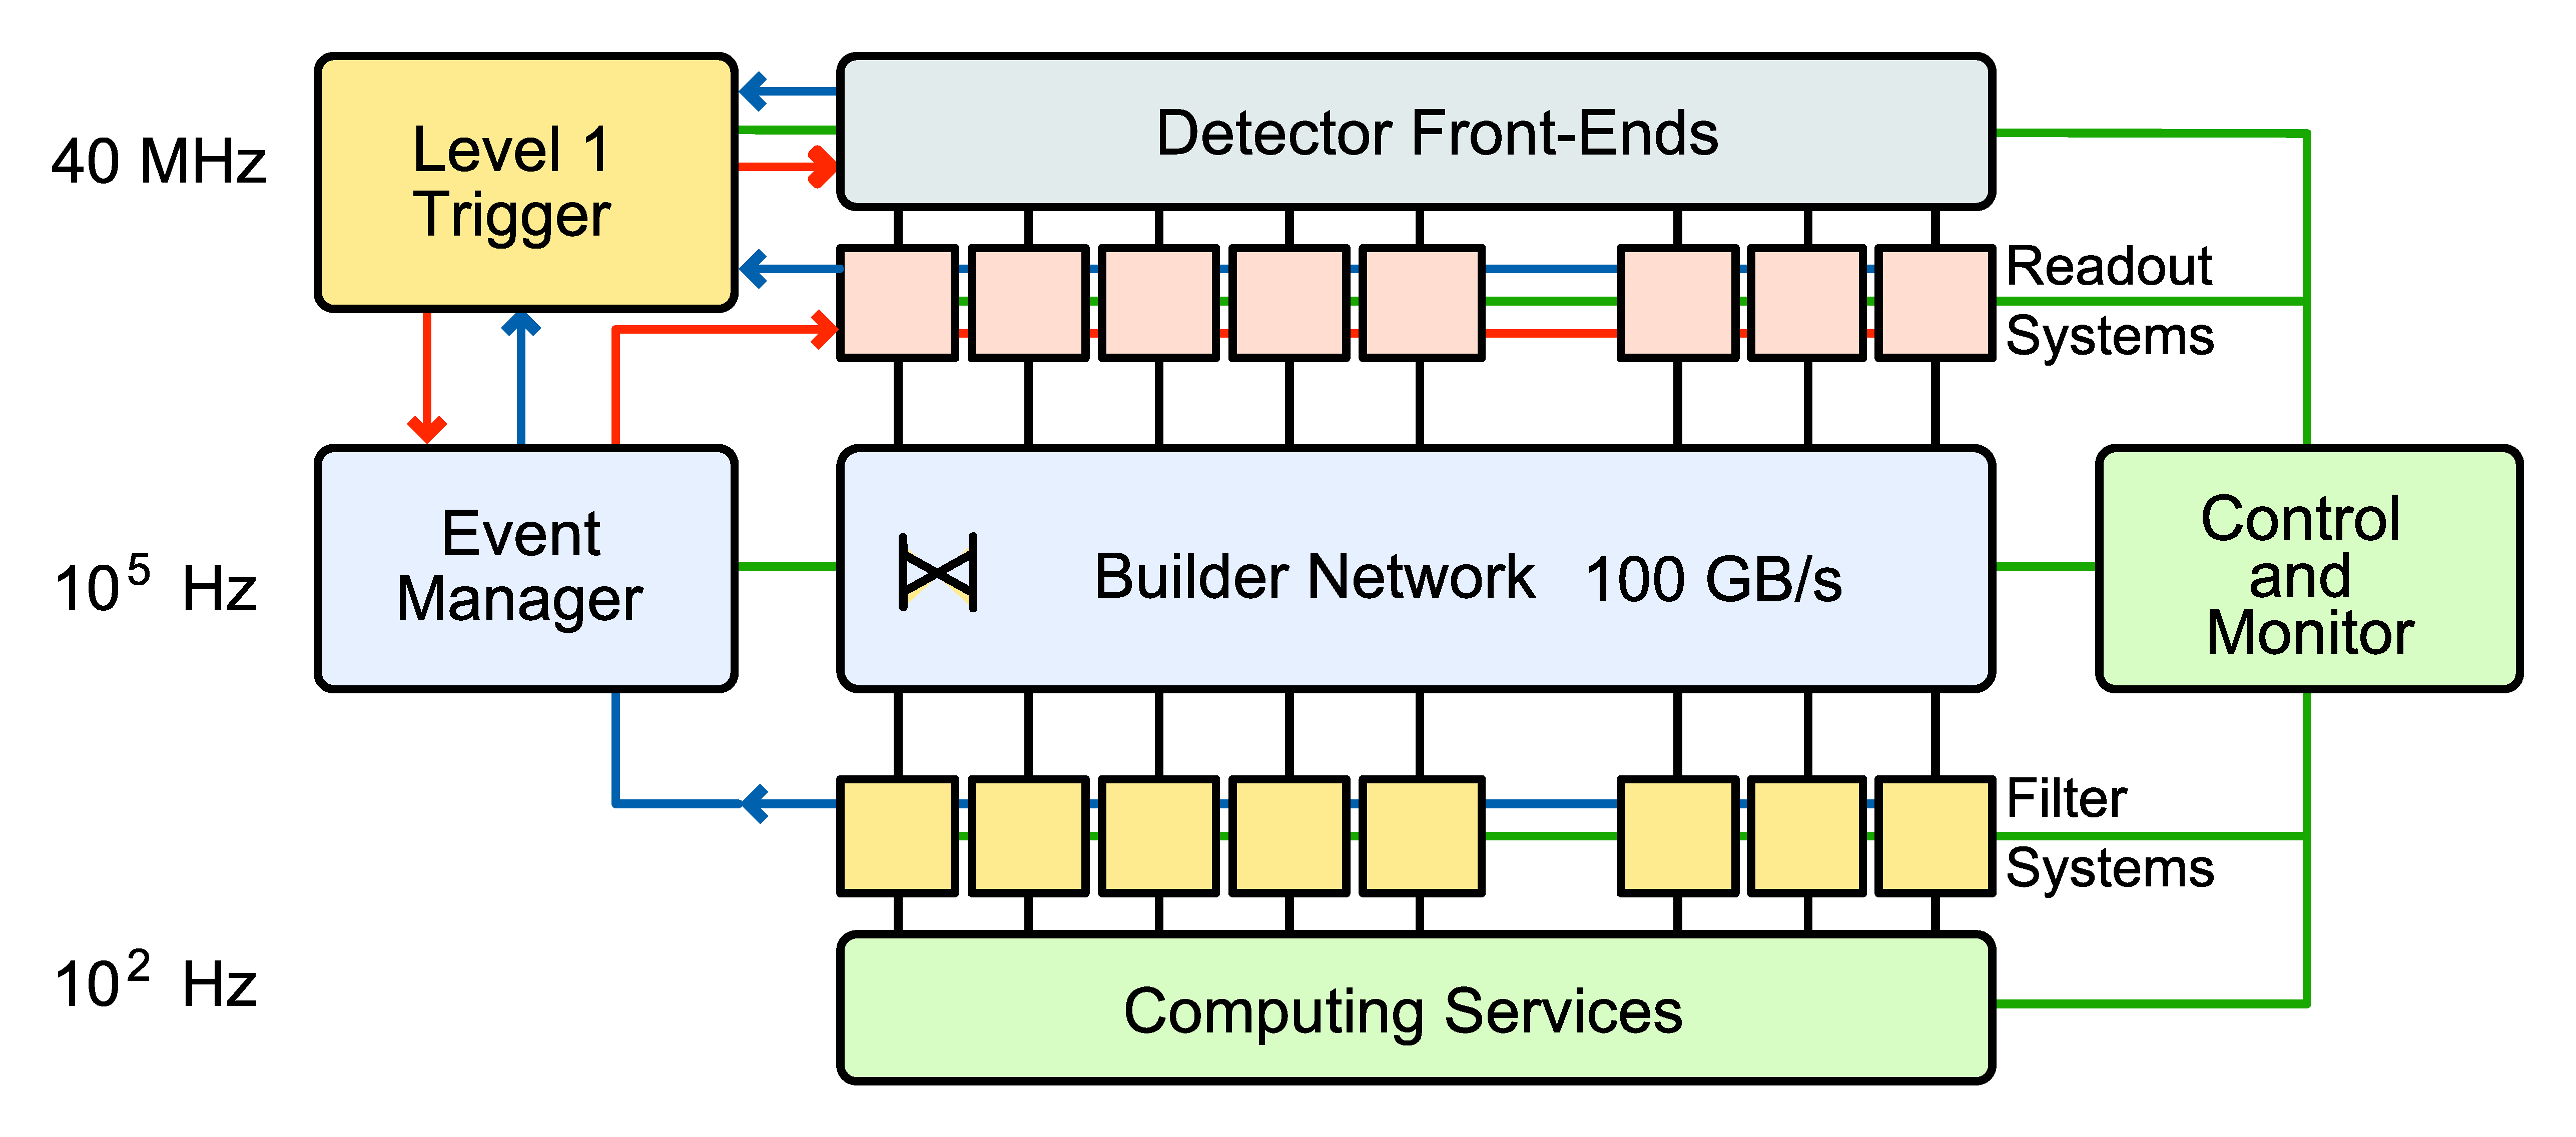
\includegraphics[width=0.7\textwidth]{chapitre2/figs/DAQ.pdf}
  \caption{Schéma de la chaîne d'acquisition de données de CMS}
  \label{fig:daq}
\end{figure}

Une fois accepté, l'événement est stocké de façon définitive dans un centre de stockage à haute redondance, le \emph{Tier-0}.

\section{Conclusion}

Tout au long de ce chapitre, on a vu comment le LHC, et le détecteur CMS, ont été pensés afin d'enrichir nos connaissances sur la physique du Modèle Standard. De nouvelles perspectives s'ouvrent dans le recherche de nouvelles physique au delà du Modèle Standard, et les mesures de précisions vont permettre de tester encore plus ce modèle. Mais pour que les analyses de physique puisse travailler, il faut dans un premier temps reconstruire les collisions, c'est-à-dire convertir les signaux électriques issus des sous-détecteurs en objets physiques (électrons, muons, \dots). Les méthodes employées par CMS sont décrites en détails dans le chapitre suivant.
\cleardoublepage\chapter{Génération, simulation et reconstruction des événements} \label{chap:reco}

Afin d'être en mesure de confronter les prédictions théoriques aux données expérimentales, il faut être capable de simuler la réponse du détecteur pour un processus donné. Pour cela, il faut tout d'abord simuler une collision entre deux protons comme si elle avait vraiment eut lieu au LHC. On utilise pour cela des outils développés spécifiquement pour cet usage, appelés générateurs d'événements Monte Carlo (MC), qui permettent de simuler l'interaction entre deux partons et de générer toutes les particules créées lors de la collision. Il est ensuite nécessaire de simuler l'interaction de ces particules avec le détecteur, afin d'extraire les réponses des différents sous-détecteurs. Ces différentes étapes sont traitées dans ce chapitre., en commençant par une description succincte des processus de génération et de simulation. La majeure partie de ce chapitre sera consacrée à la description des algorithmes de reconstruction des particules, cruciaux pour les analyses de physique.

\section{Génération des événements}

\fxerror{Compléter cette partie - 1 ou 2 pages de plus}

%Afin d'extraire des informations sur les observables physiques, telles que les sections efficaces par exemple, on utilise un développement perturbatif. En effet, la probabilité de transition d'un état initial $\ket{i}$ à un état final $\ket{f}$ est calculée en utilisant la règle d'or de Fermi. Cette règle est obtenue grâce à la théorie des perturbations, en considérant que le temps nécessaire à l'interaction est bien plus petit que le temps nécessaire à l'observation.

%La précision du résultat dépend de l'ordre du calcul. Le premier ordre, celui le plus simple à calculer, correspond à un nombre de vertex de 2, et est appelé calcul à l'arbre (ou \emph{LO}, pour \emph{Leading Order}).

\subsection{L'événement dur}

Lors d'une collision entre deux protons, seul les constituants (les partons: quarks et gluons) vont interagir, chacun emportant une certaine fraction $x$ de l'impulsion totale du proton incident. Afin d'extraire des informations sur les observables physiques, telles que les sections efficaces par exemple, on utilise un développement perturbatif à plusieurs ordres.

L'événement dur est décrit de façon analytique en utilisant ce développement perturbatif. Le générateur détermine grâce à un ensemble de règles, appelées règles de Feynman, la matrice de transition entre l'état initial et l'état final. Le calcul au premier ordre (LO, \emph{Leading Order}) est disponible pour les processus les plus importants du Modèle Standard, implémenté dans des programmes tel que \texttt{MadGraph} \citep{madgraph} par exemple. Les simulations aux ordres supérieurs deviennent extrêmement complexes, et sont disponibles seulement pour un petit nombre de processus et ont été implémenté dans des programmes particuliers comme \texttt{Powheg} \citep{Alioli:2010xd}, \texttt{MC@NLO} \citep{1126-6708-2002-06-029}, etc.

La section efficace partonique $\sigma_{ij} \rightarrow X$, avec $i, j = \Pgluon, \Pquark$ et $X$ un état final choisit, peut s'exprimer de la façon suivante :
\begin{align}
  \sigma_{X} &= \sum_{ij} \int \displaylimits_0^1 \int \displaylimits_0^1 f_i\left( x_i, \mu^2 \right) f_j\left(x_j, \mu^2\right) \sigma_{ij \rightarrow X}\, \mathrm{d}x_i \mathrm{d}x_j \notag \\
  \sigma_{ij \rightarrow X} &\propto \int \prod \displaylimits_{k = 1}^{N} \frac{\mathrm{d}^3p_k}{\left( 2 \pi \right)^2 2 E_k} \delta^4\left( p_i + p_j - \sum_{k = 1}^{N} p_k \right) \left| \mathcal{M}_{fi} \right|^2 \label{eq:section_efficace}
\end{align}
où $f_{i, j}$ est la densité de probabilité partonique (détaillée \cref{sec:pdf}), $x_i$ la fraction d'impulsion emportée par le parton $i$, $\mu^2$ l'échelle d'énergie du processus et $\mathcal{M}_{fi}$ l'élément de matrice de transition entre l'état initial $i$ et l'état final $f$. L'élément de matrice est calculé jusqu'à un ordre donné, limité par l'ordre auquel les calculs théoriques ont pu être mené, et l'intégration est effectuée numériquement selon une méthode d'intégration Monte Carlo.

\begin{figure}[tbp]
    \centering
    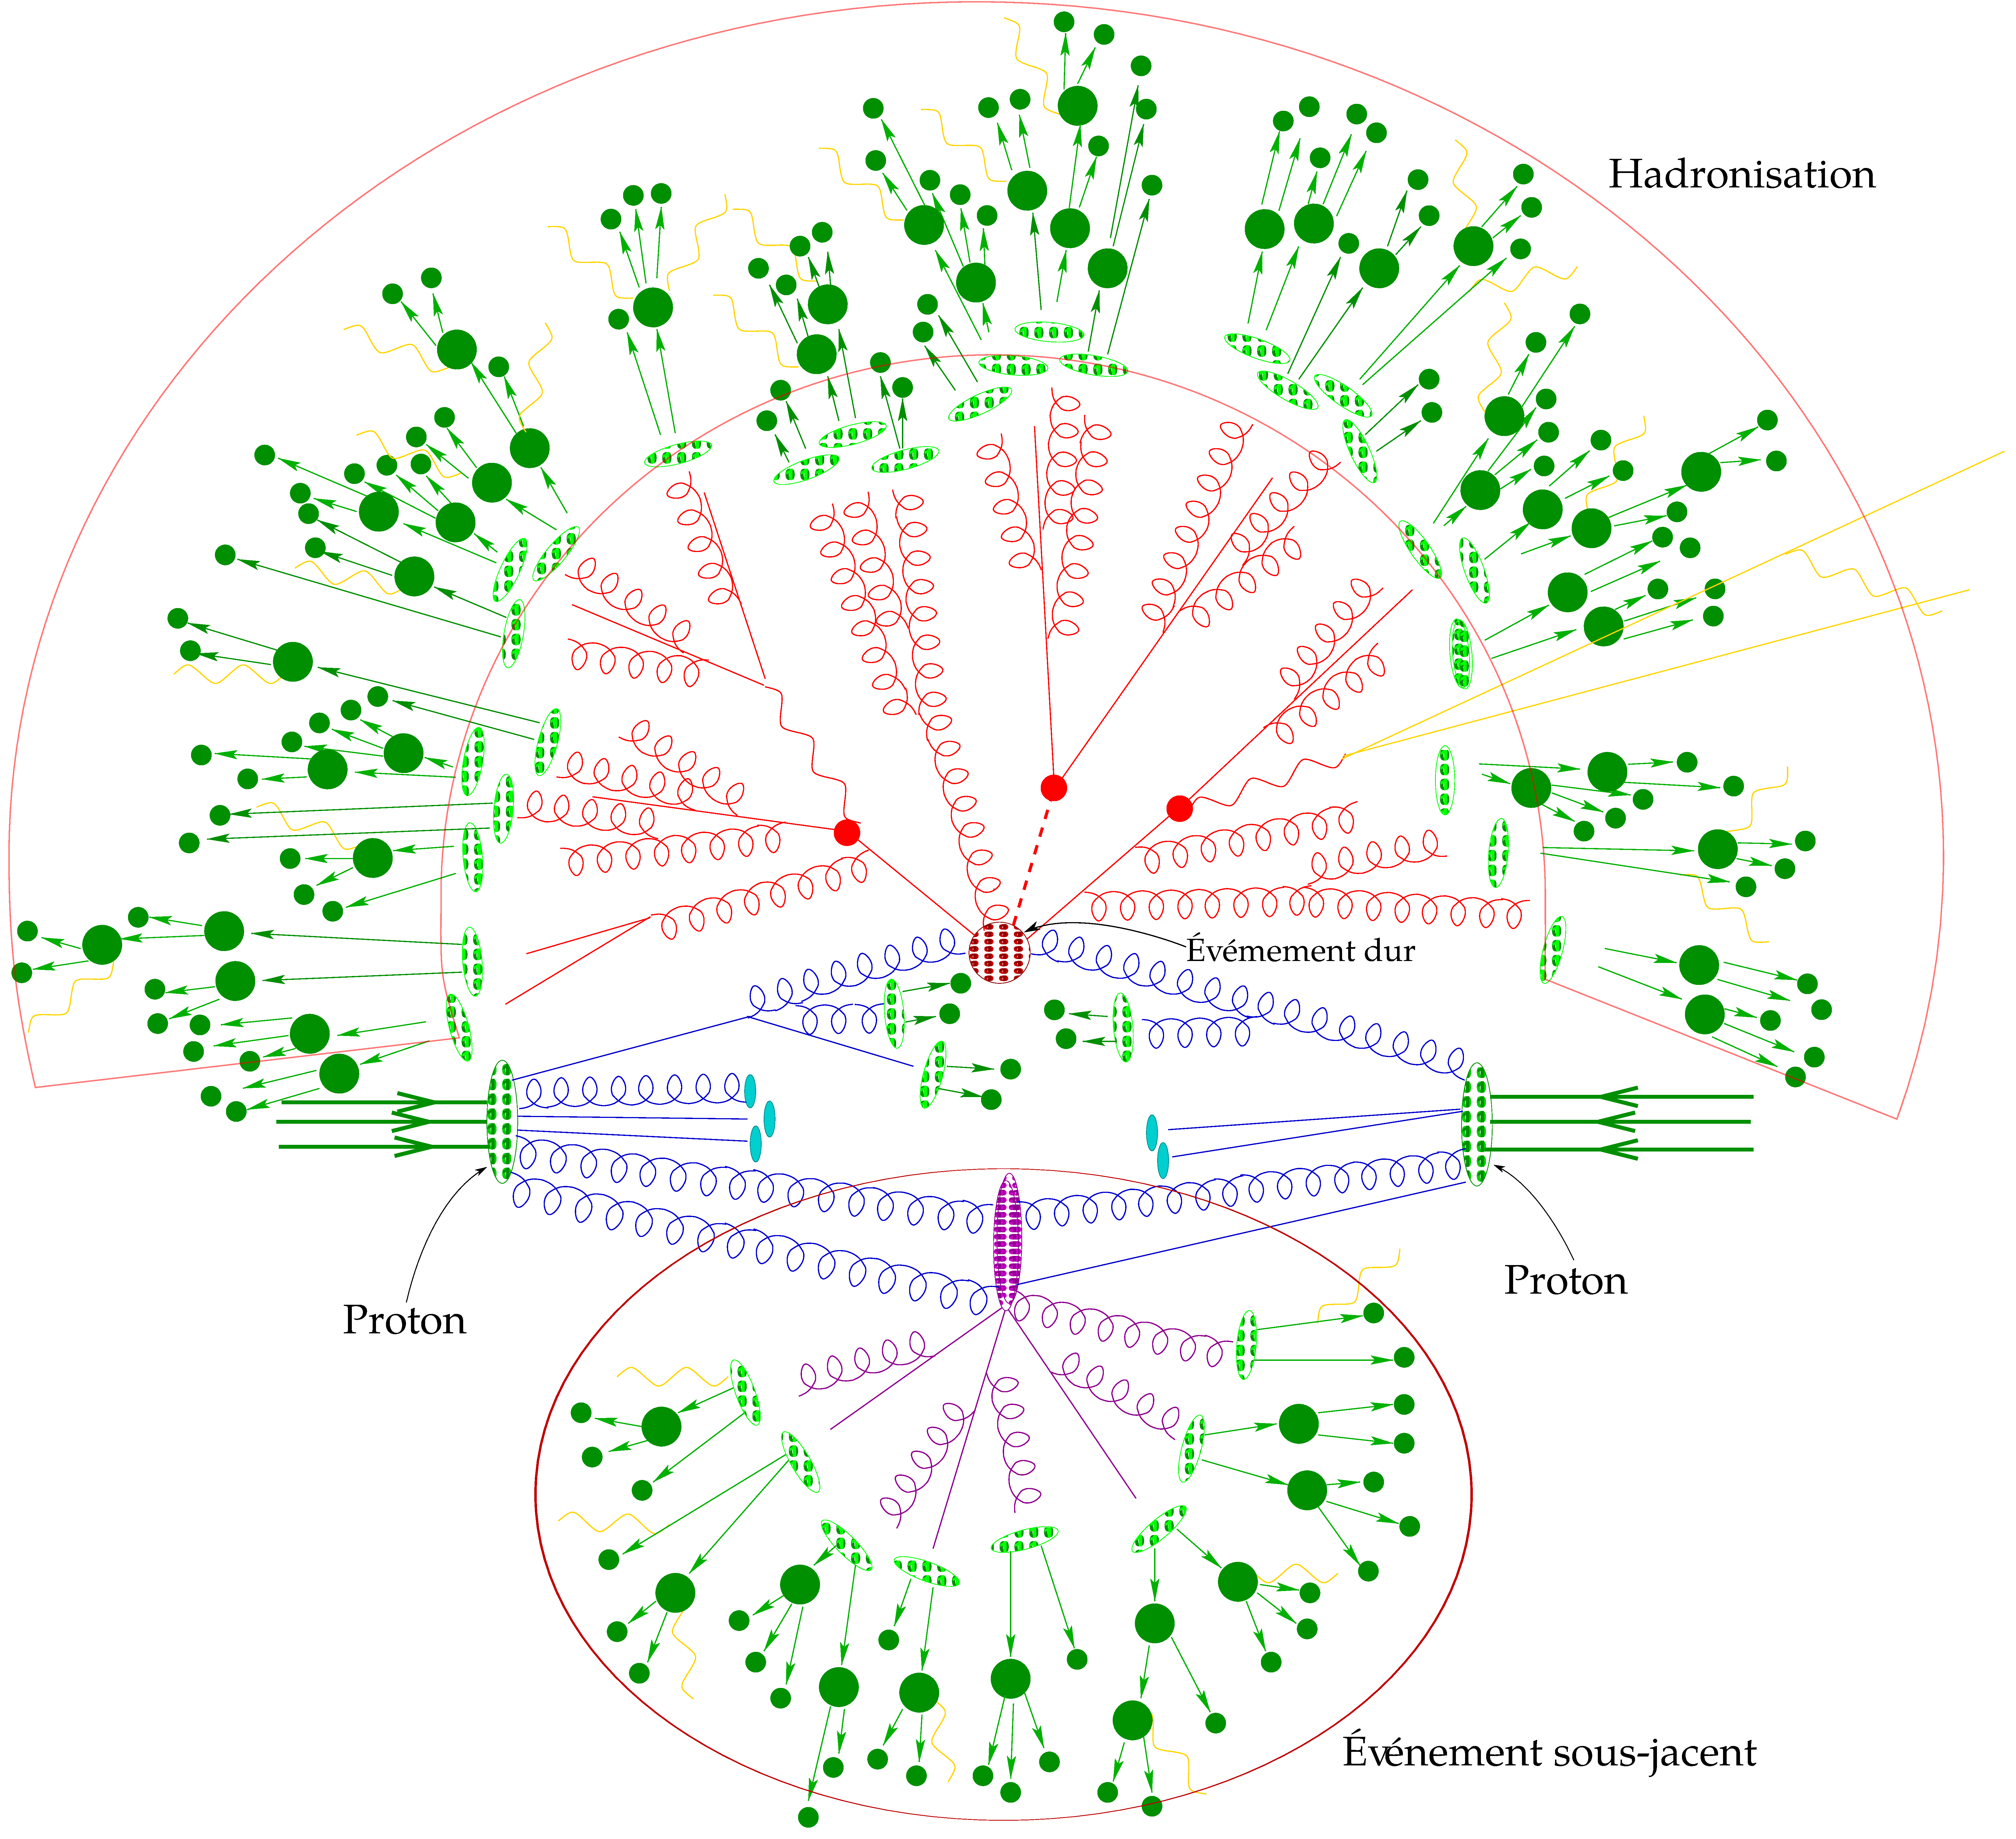
\includegraphics[width=0.99\textwidth]{chapitre3/figs/parton_shower_legend.pdf}
    \caption{Représentation graphique d'une collision de deux protons simulée à l'aide d'un générateur. L'événement dur (au centre, en rouge) est produit par l'interaction de deux partons. Les trois particules produites (rond rouge plein) se désintègrent. C'est à ce niveau qu'intervient l'hadronisation.Des radiations de photons (jaune) ont été rajoutées à chaque étape.}
    \label{fig:parton_shower}
\end{figure}

On obtient en sortie du générateur le quadrivecteur impulsion de chaque particule produite lors de l'événement dur.

\subsection{Densité de probabilité partonique (PDF)} \label{sec:pdf}

Le calcul des sections efficaces des processus faisant intervenir des hadrons nécessite la connaissance des densités de probabilité partonique (PDF) $f_i\left( x, \mu^2 \right)$, qui représente la probabilité de trouver un parton $i$ au sein du hadron, emportant une fraction d'impulsion $x$ lors d'un processus à l'échelle d'énergie $\mu^2$. Ces fonctions ne peuvent pas être déterminées par des calculs perturbatifs, mais sont obtenus à partir d'ajustement sur les données expérimentales. Les principales sources de données proviennent des mesures de l'expérience HERA, permettant de sonder la structure du proton en faisant collisionner des protons avec des électrons. L'étude de la production des jets au Tevatron et au LHC contribue également considérablement à la connaissance des PDFs des gluons. Malheureusement, l'échelle d'énergie du LHC permet d'obtenir des collisions à très petit $x$ et très grand $\mu^2$, gamme non couverte par les données expérimentales : il est nécessaire d'extrapoler les PDFs, augmentant ainsi les incertitudes liées aux PDFs.

\smallskip

Deux groupes principaux fournissent les PDFs, CTEQ \citep{Owens:2012bv} et MSTW \citep{Martin:2009iq}, qui publient régulièrement des nouvelles PDFs tenant compte des dernières mesures. La \cref{fig:cj12} présente les PDFs pour divers partons issues du jeu de PDFs CJ12, pour une échelle en énergie $\mu^2 = \SI{100}{\GeV}$.

\begin{figure}[tbp]
  \centering
  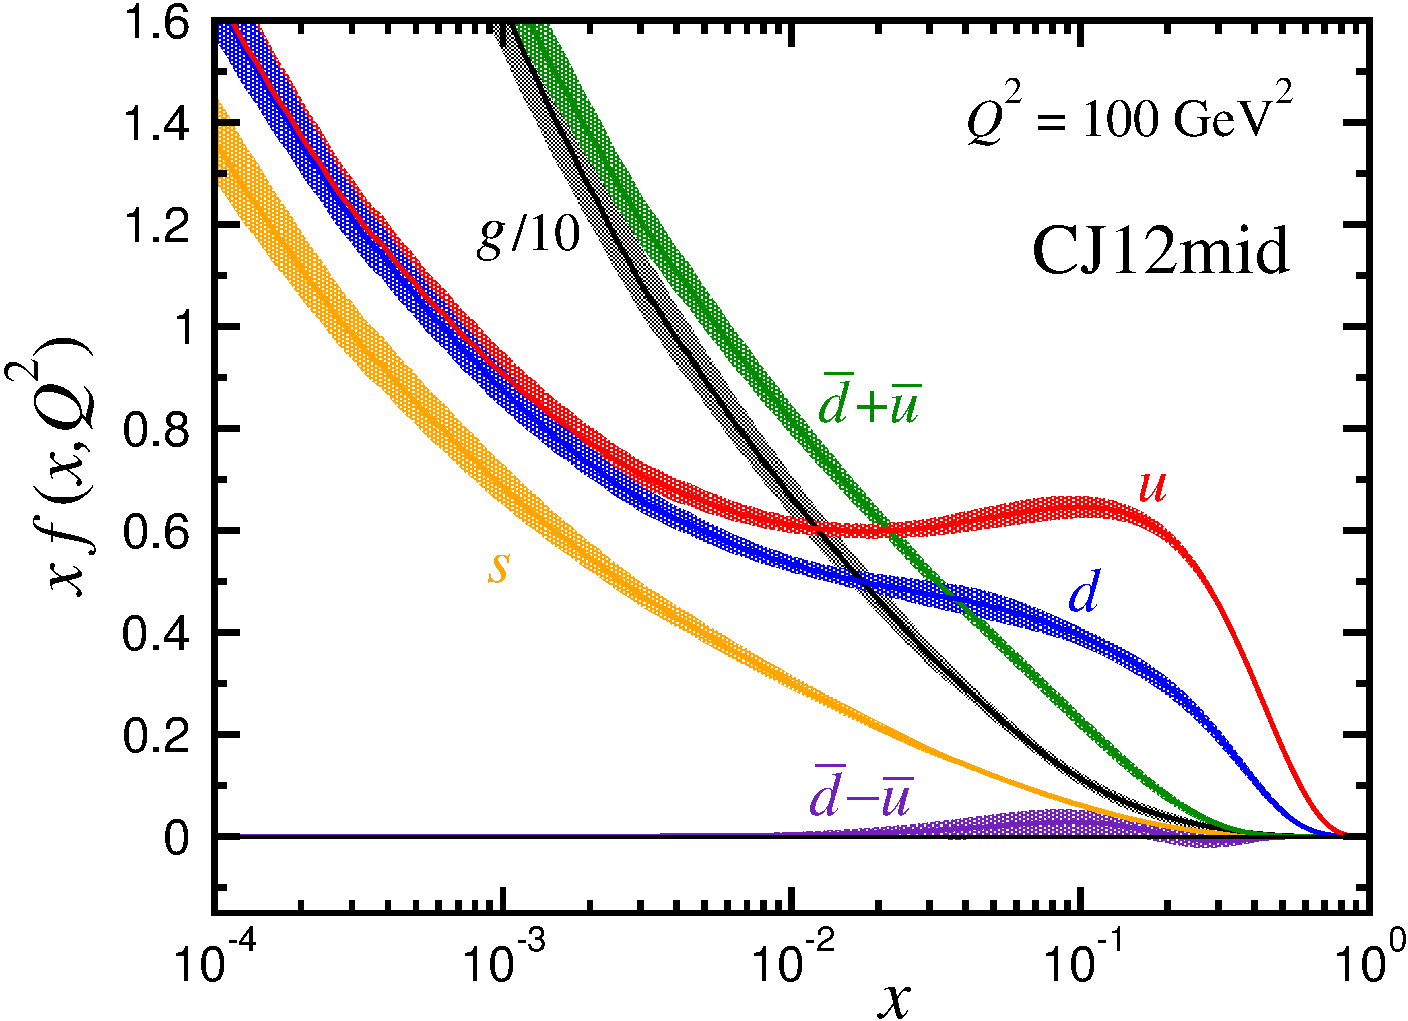
\includegraphics[width=0.6\textwidth]{chapitre3/figs/Fx_errl.pdf}
  \caption{PDFs pour divers partons issues du jeu de PDFs CJ12 \citep{Owens:2012bv}.}
  \label{fig:cj12}
\end{figure}


\subsection{L'hadronisation des partons : la gerbe partonique}

La majeure partie des particules produites lors de l'événement dur ne sont pas stables, et vont se désintégrer avant d'être détectée. Le cas des partons est encore plus complexe. Dans un premier temps, ils vont radier des gluons \emph{via} interaction forte, créant ainsi une gerbe partonique. Ensuite, étant des particules colorées, ils doivent obligatoirement se lier à d'autres partons afin de former des états non colorés (hadrons), c'est-à-dire neutre du point de vue de l'interaction forte. Ce processus est appelé hadronisation, et a lieu environ \SI{5e-24}{\s} après la production de la particule. Les hadrons ainsi formés peuvent ou non être stable. Lors de leur désintégration, les nouvelles particules produites vont à leur tour s'hadroniser. On obtient ainsi une cascade de désintégrations et d'hadronisations.

Ces effets sont très complexe à simuler, puisque à l'échelle d'énergie où ils se produisent, la QCD devient non-perturbative. Des programmes dédiés permettent néanmoins de simuler toute la chaîne d'hadronisation des particules, chacun utilisant des algorithmes spécialisés afin de simuler au mieux le développement de la gerbe partonique et de la chaine d'hadronisation. Parmi ces programmes, on peut citer \texttt{Pythia} \citep{pythia} et \texttt{Herwig} \citep{Corcella:2000bw}.

\section{Simulation des événements}

Une fois l'hadronisation terminée, on dispose d'une liste de particules créées lors de la collision. Avant de pouvoir comparer les prédictions théoriques aux données collectées, il reste encore à simuler la réponse du détecteur. Deux approches sont possibles : une simulation détaillée, basée sur \texttt{Geant\;4} \citep{Agostinelli2003250}, mais très coûteuse en temps de calcul, et une moins détaillée, mais extrêmement plus rapide. Chaque méthode permet, grâce à des algorithmes différents, de simuler :
\begin{itemize}
    \item Le passage des particules dans le détecteur
    \item Les courbures des trajectoires des particules chargées par le champ magnétique
    \item Les gerbes électromagnétiques et hadroniques
    \item Les interactions particules - matières
    \item La réponse électrique des détecteurs
\end{itemize}

En plus de la liste ci-dessus, la simulation est aussi responsable de la désintégration des particules instables produites lors de la génération. En effet, la notion de stabilité dépend de l'échelle de temps considérée : une particule ne se désintégrant pas avant un temps $\tau$ est considérée comme stable. Ainsi, une particule peut être vue stable par le générateur Monte Carlo, mais instable par la simulation. Cette particule se désintègre donc à l'intérieur du détecteur, et cet effet doit être pris en compte pour une simulation complète.

\medskip

On décrit rapidement les deux méthodes de simulation ci-dessous.

\subsection{La simulation complète du détecteur}

Cette simulation repose sur une description extrêmement précise du détecteur. Ainsi, une réplique détaillée du détecteur est créée en 3-dimensions, comprenant même le câblage électrique des divers sous-détecteurs. Ce modèle est ensuite utilisé par le logiciel \texttt{Geant\;4}, qui va simuler la propagation, l'interaction, les diffusions multiples et la réponse des détecteurs pour chacune des particules créées lors de la collision. C'est une simulation très coûteuse en temps de calcul : la simulation d'un événement peut atteindre jusqu'à 2 minutes selon la complexité de l'état final.

\subsection{La simulation rapide du détecteur}

Une solution de simulation plus rapide existe au sein de la collaboration. Développée spécialement pour CMS \citep{1742-6596-219-3-032053}, cette simulation utilise une géométrie simplifiée du détecteur, et considère que les matériaux des sous-détecteurs ont une densité constante. La simulation des interactions au sein des divers sous-détecteurs est approximée en se basant sur les simulations complètes du détecteur. Tout en étant beaucoup rapide (environ \SI{200}{\ms} par événement), cette simulation permet de reproduire la plupart des observations avec une erreur de l'ordre du pourcent.  Elle est beaucoup utilisée pour les études de mise-à-jour des détecteurs, où il est nécessaire de pouvoir simuler très rapidement l'effet d'une modification du détecteur sur les observables physiques.

\section{Reconstruction des événements}

La reconstruction d'un événement est effectuée de façon identique, que ça soit de la simulation ou une prise de données réelle. En effet, la simulation du détecteur fournie en sortie les signaux électriques des sous-détecteurs, de façon identique à ce qui se passe lors des vraies collisions.

\subsection{L'algorithme \emph{Particle-Flow} (PF)}

CMS utilise un algorithme spécialisé pour reconstruire les objets physiques : l'algorithme du \emph{particle-flow} \citep{pf,cms_pf_2,cms_pf_jets,cms_pf_leptons}. En utilisant l'information de tous les sous-détecteurs pour reconstruire l'événement, cet algorithme permet d'améliorer significativement la résolution des particules reconstruites, et s'avère être un moyen efficace de contrebalancer les faiblesses du HCAL : on peut en effet utiliser l'excellente performance du trajectographe pour aider à la reconstruction des hadrons chargés.

Le \emph{particle-flow} permet de reconstruire les 5 types de particules stables détectées par CMS : les électrons, les muons, les photons, et certains hadrons neutres et chargés. Ces particules sont ensuite utilisées comme des briques élémentaires pour reconstruire des objets plus complexe, comme les jets. Ces briques étant ensuite utilisées par les analyses de physique, il est primordial que le \emph{particle-flow} possède une efficacité de reconstruction la plus haute possible, tout en ayant un taux de fausse identification le plus faible possible. Ces contraintes ont conduit a l'élaboration d'algorithmes dédiés de trajectographie et de calorimétrie, détaillés ci-dessous.

\subsubsection{Trajectographie itérative} \label{sec:tracks_reconstruction}

L'impulsion des hadrons est mesurée avec une résolution bien meilleure par le trajectographe que par les calorimètres. Comme près de \sfrac{2}{3} de l'énergie d'un jet est dû à la présence de hadrons chargés, le trajectographe joue un rôle majeur dans la performance du \emph{particle-flow}.

Afin de reconstruire les trajectoires des particules avec une grande efficacité, tout en conservant un taux de faux minimal, une procédure itérative \citep{cms_tracks}, basée sur un filtre de Kalman (KF), est employée. La reconstruction commence en utilisant seulement les \emph{hits} des deux premières couches du détecteur à pixels, ainsi que la position du vertex primaire. C'est ce qu'on appelle la graine de l'algorithme. On cherche ensuite à compléter la trajectoire en utilisant les \emph{hits} des autres couches du trajectographe. Les contraintes lors de cette première étape sont vraiment fortes, ce qui conduit à une efficacité de reconstruction moyenne, mais à un très faible taux de faux.

Avant l'étape suivante, les \emph{hits} associés de façon certaine à une trajectoire sont enlevés de la liste des \emph{hits} disponibles, et on réitère ensuite la même procédure en relâchant un peu les contraintes, ce qui permet d'améliorer l'efficacité de reconstruction, tout en gardant un taux de faux très faible grâce à la réduction du nombre de combinaison. Après la troisième itération, on obtient une efficacité de reconstruction de \SI{99.5}{\%} pour les muons isolés et de plus de \SI{90}{\%} pour les hadrons chargés. Pour les quatrième et cinquième itérations la contrainte sur le point d'interaction est relâchée, ce qui permet de reconstruire les trajectoires des hadrons chargés secondaires ayant un vertex d'interaction déplacé.

Grâce à cet algorithme de trajectographie itérative, la trajectoire d'une particule chargée ne laissant que 3 \emph{hits}, avec un $p_T$ de seulement \SI{150}{\MeV} et un vertex de production éloigné de plus de \SI{50}{\cm} de l'axe du faisceau est reconstruite avec un taux de faux de l'ordre du pour-cent. On peut voir figure \ref{fig:iterative_tracking_eff} l'efficacité de reconstruction des trajectoires grâce à l'utilisation de l'algorithme de trajectographie itératif.

\begin{figure} \centering
  \subcaptionbox{\label{fig:tracking_eff_mu}}[0.45\textwidth]{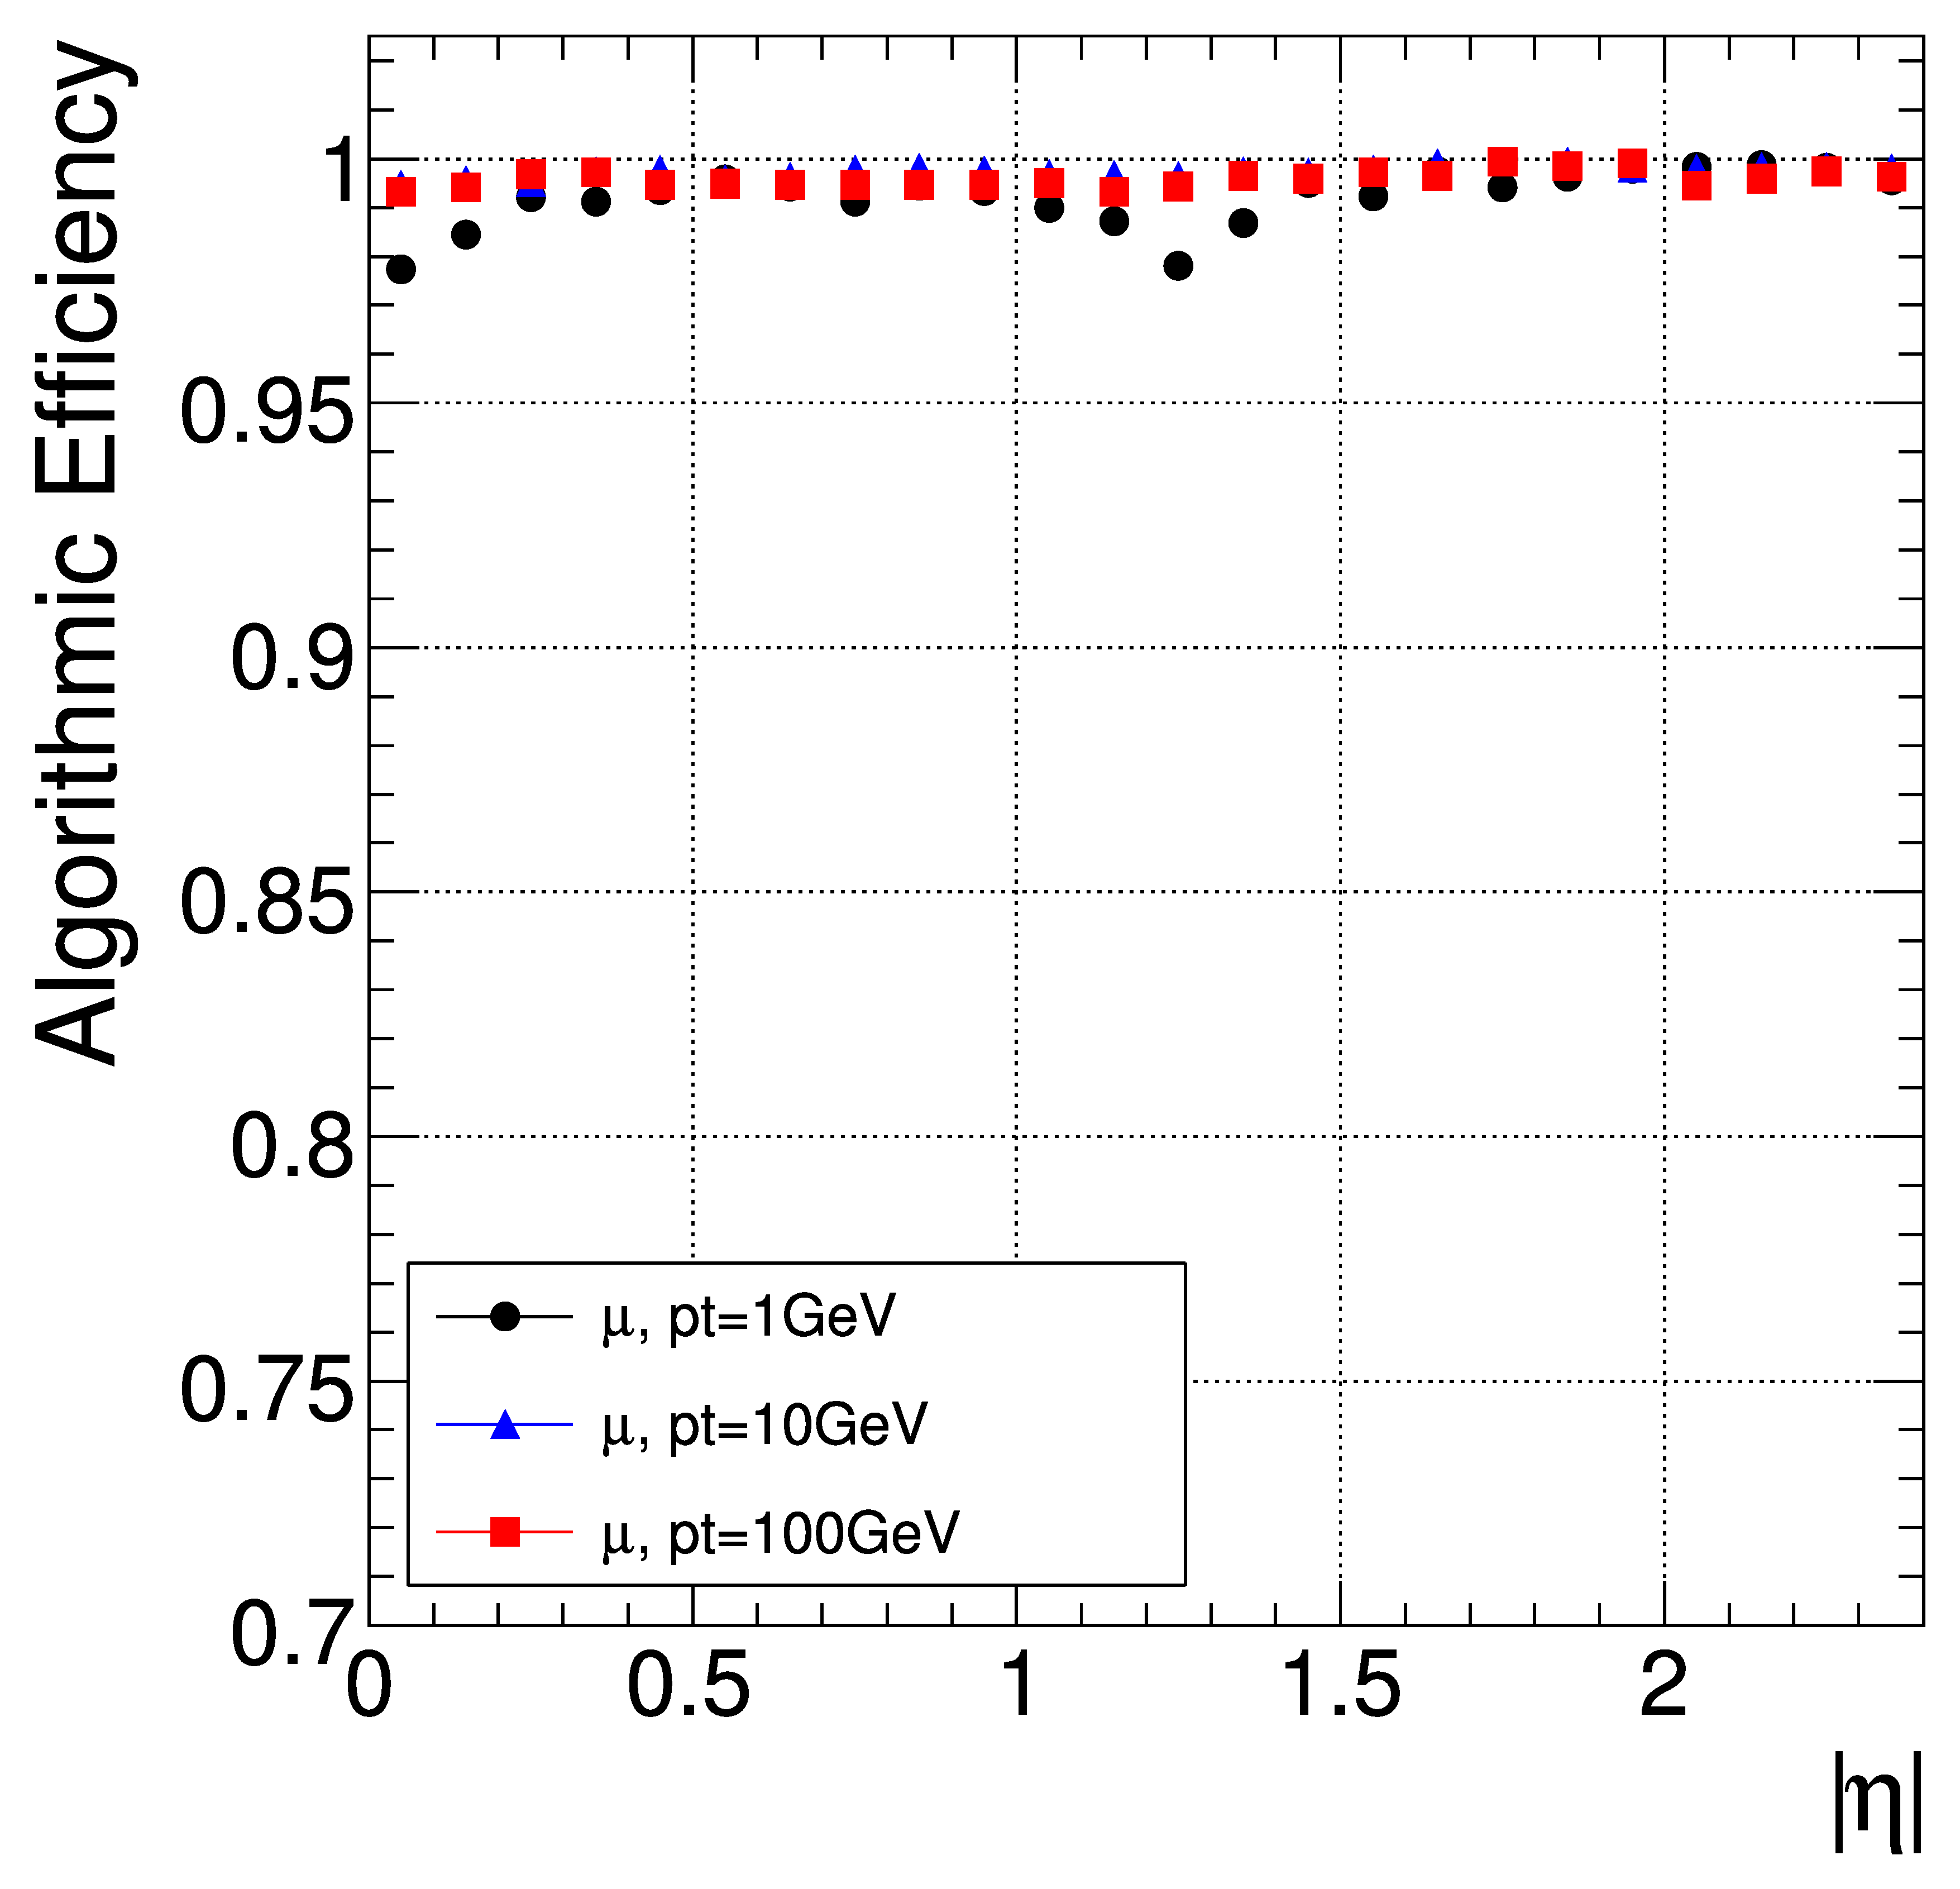
\includegraphics[width=0.45\textwidth]{chapitre3/figs/iterative_tracking_mu.pdf}}\hfill
  \subcaptionbox{\label{fig:tracking_eff_pi}}[0.45\textwidth]{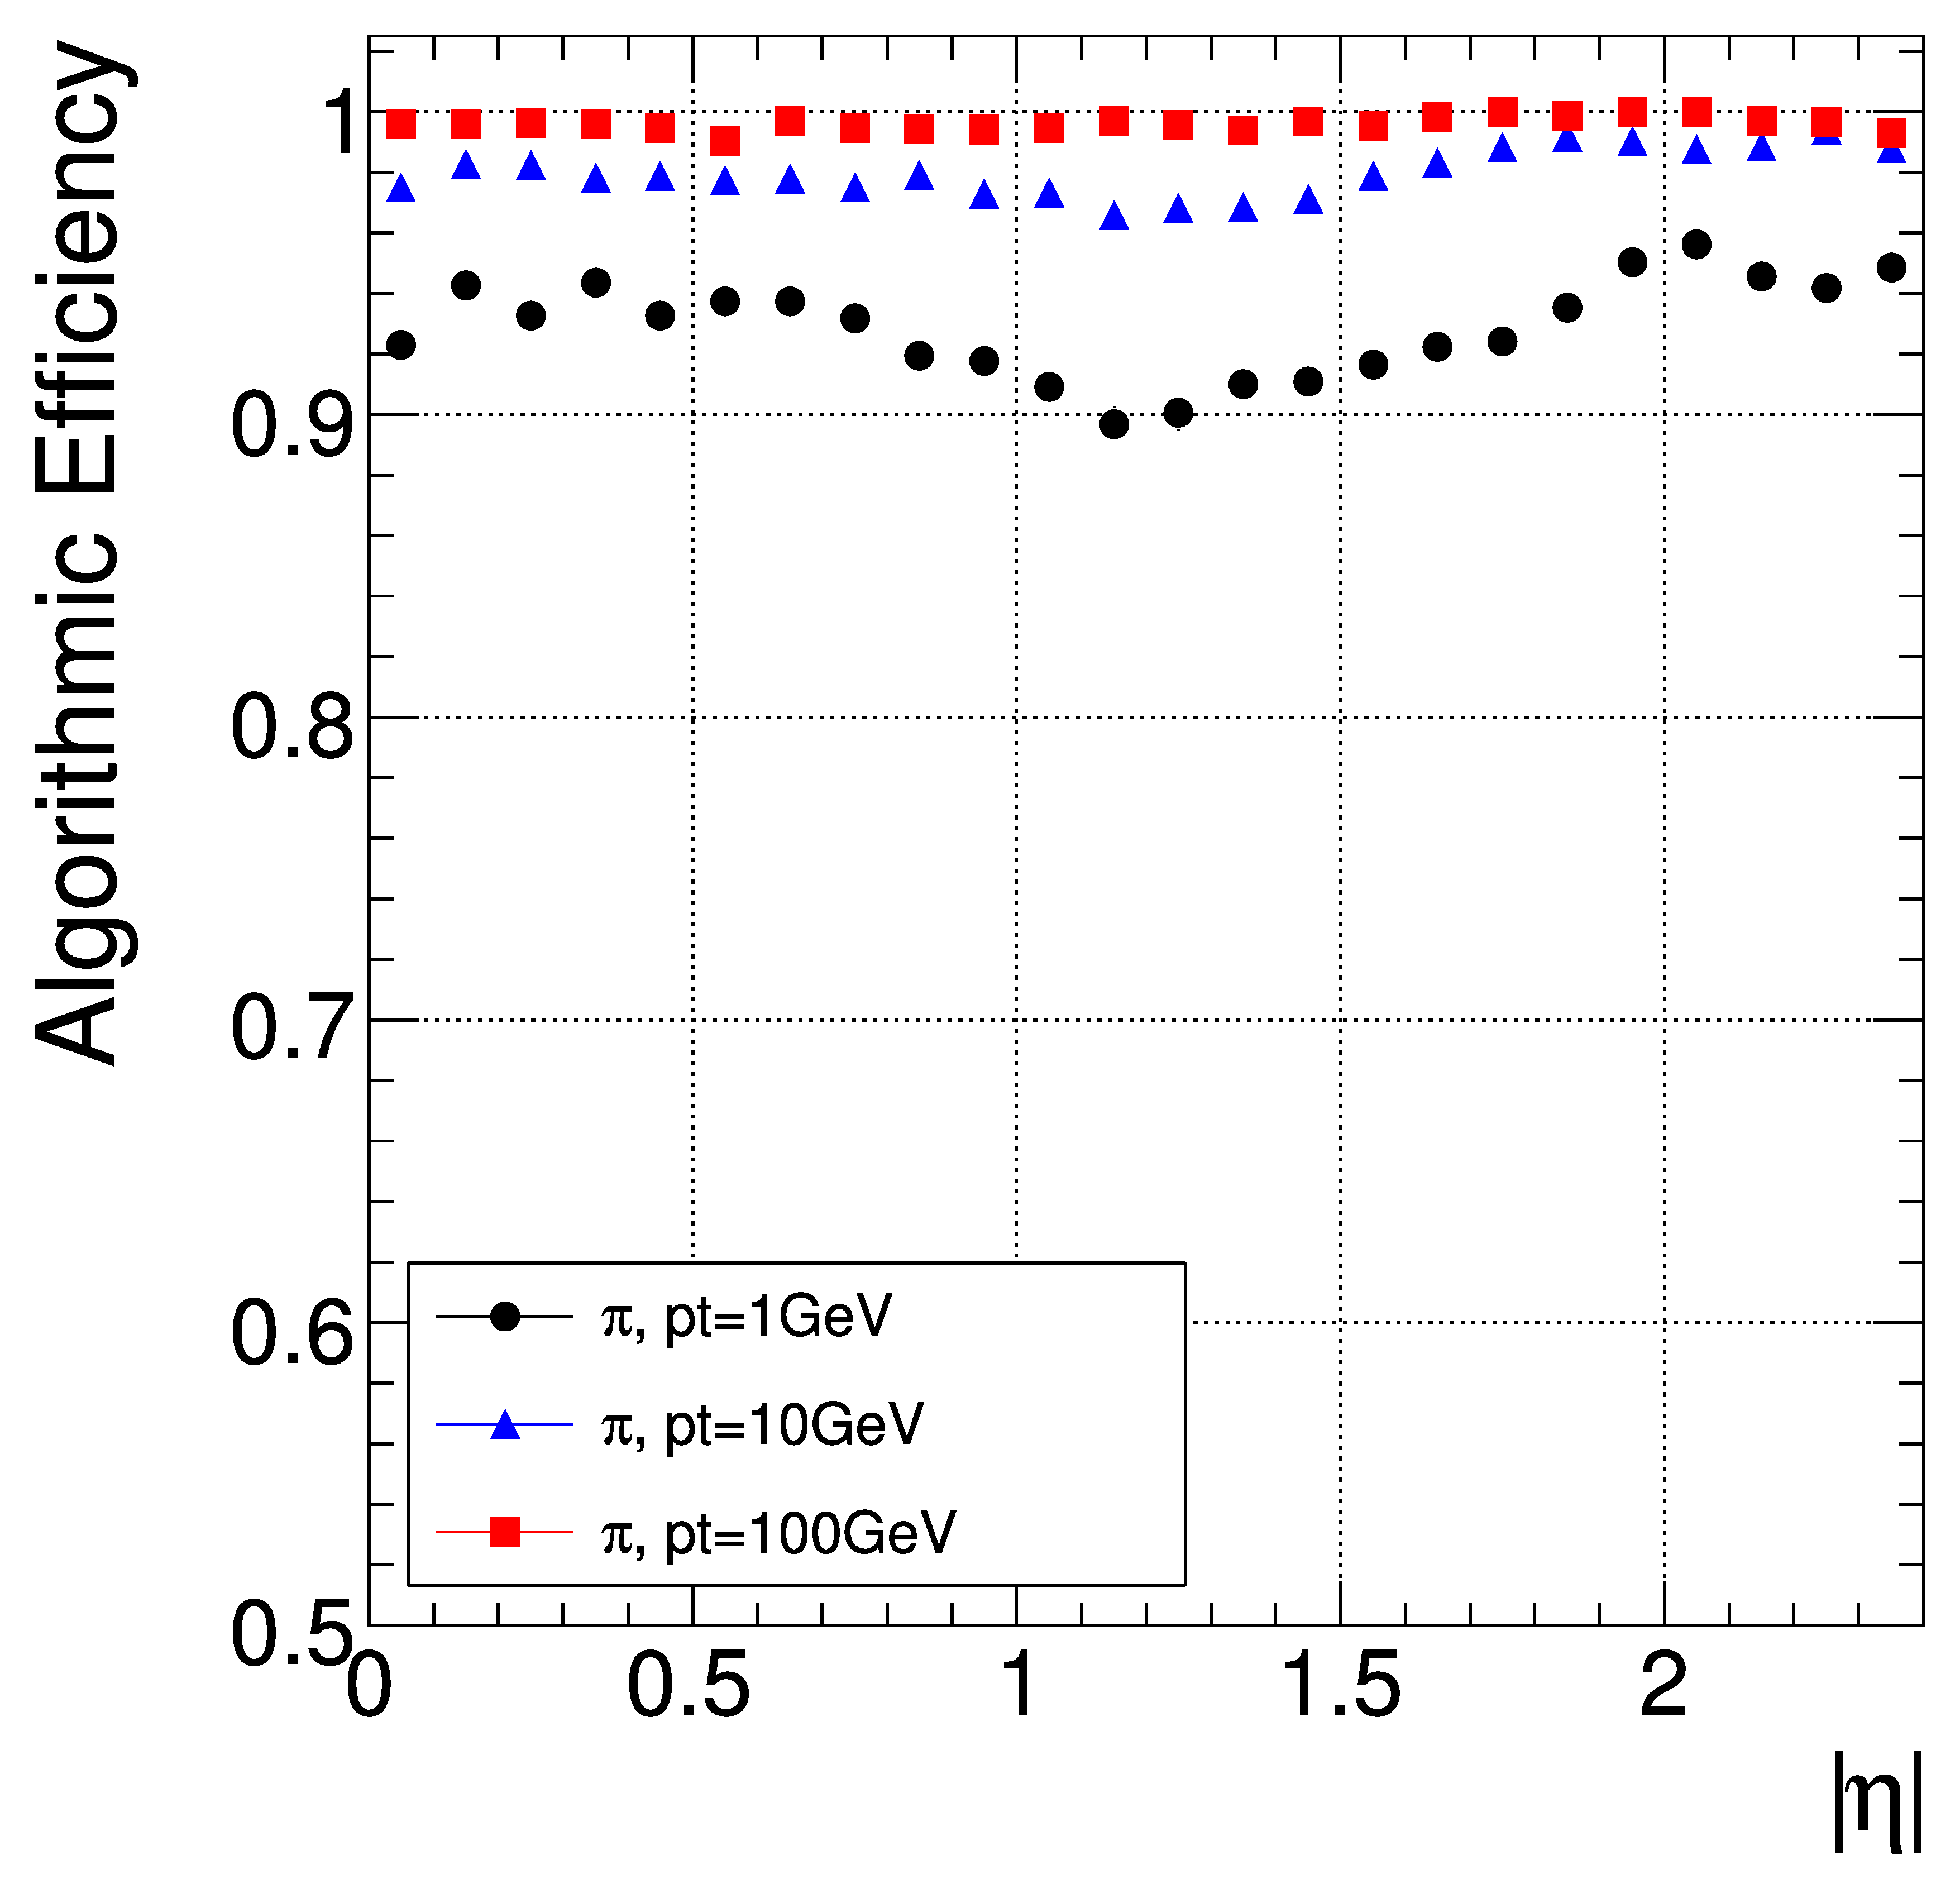
\includegraphics[width=0.45\textwidth]{chapitre3/figs/iterative_tracking_pi.pdf}}
  \caption{Efficacité de reconstruction des trajectoires pour des muons (\subref{fig:tracking_eff_mu}) et pour des pions (\subref{fig:tracking_eff_pi}).}
  \label{fig:iterative_tracking_eff}
\end{figure}

\subsubsection{Agglomération calorimétrique}

Un algorithme d'agglomération calorimétrique cherche à atteindre 4 buts :
\begin{enumerate}
  \item Mesurer l'énergie et la direction des particules neutres (photon, hadrons neutres).
  \item Séparer les dépôts d'énergies des particules neutres de ceux des particules chargées.
  \item Reconstruire les électrons et le rayonnement Bremsstrahlung associé.
  \item Aider à la mesure de l'énergie des hadrons chargés pour lesquels la trajectoire n'a pas été bien reconstruite (hadrons de bas \pt).
\end{enumerate}

L'algorithme spécifique développé pour le \emph{particle-flow} permet d'atteindre une très haute efficacité de reconstruction, tout en gardant un grand pouvoir de séparation des dépôts d'énergie. L'agglomération est effectuée de façon séparée dans chaque sous-calorimètre (tonneau du ECAL, tonneau du HCAL, bouchons du ECAL et HCAL, \ldots), et ce en trois phases.

\medskip

\begin{figure}
  \subcaptionbox{\label{fig:calo_topo}}[0.45\textwidth]{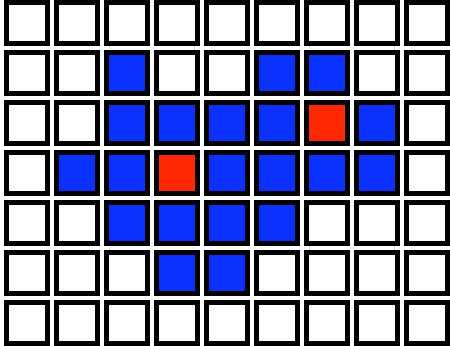
\includegraphics[width=0.45\textwidth]{chapitre3/figs/calo_topoclus_seeds.pdf}}\hfill
  \subcaptionbox{\label{fig:calo_depth}}[0.45\textwidth]{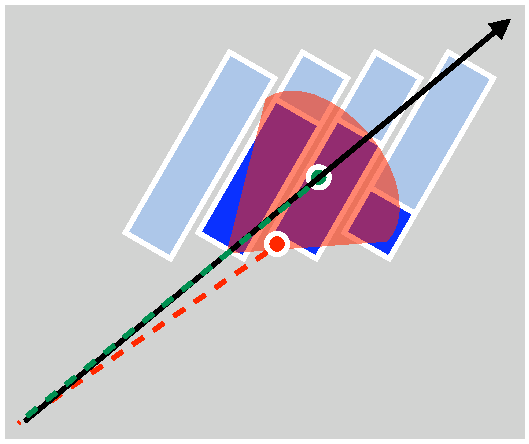
\includegraphics[width=0.45\textwidth]{chapitre3/figs/calo_depthcor.pdf}}
  \caption{Agglomérat topologique contenant deux graines (\subref{fig:calo_topo}) et détermination de la profondeur du dépôt d'énergie (\subref{fig:calo_depth}). En rouge, la position déterminée sans tenir compte de la profondeur biaise \aeta. En vert, la profondeur est correctement estimée.}
\end{figure}

Premièrement, on identifie les graines de l'algorithme comme les cellules calorimétrique où l'énergie dépasse un certain seuil, fixé à une valeur supérieure au niveau de bruit du détecteur. Les cellules en contact avec une graine (4 ou 8 suivant la configuration) ne peuvent pas devenir des graines à leur tour. On construit ensuite des "agglomérats topologiques", en partant des graines et en agrégeant les cellules avec au moins un côté en commun avec la graine et avec une énergie au dessus d'un seuil, fixé comme deux fois la déviation standard du bruit électronique dans le ECAL (\SI{80}{\MeV} dans le tonneau, \tilde \SI{300}{\MeV} dans les bouchons) et à \SI{800}{\MeV} dans le HCAL. Il peut y avoir plusieurs graines dans un même agglomérat topologique. Dans ce cas, le partage de l'énergie entre chaque graine est effectuée selon la distance entre la cellule et la graine, en considérant que les gerbes électromagnétiques déposent leur énergie selon un profil gaussien, dont la largeur ne dépend pas de l'énergie.

\medskip

La position de l'agrégat est déterminée à partir de la graine et des 4 ou 8 cellules voisines, à l'aide de la formule
\begin{align*}
  X &= \frac{ \sum_i{w_i X_i} }{ \sum_i{w_i} }\text{, avec } w_i = \ln{\frac{E_i}{E_{th}}}
\end{align*}
avec $X = x, y$ ou $z$, $X_i$ la position de la cellule $i$, $E_i$ l'énergie de la cellule $i$, et $E_{th}$ le seuil d'énergie. Dans le cas où l'agrégat ne compte qu'une seule graine, toutes les cellules de l'agrégat sont utilisées pour calculer la position. Afin de ne pas introduire de biais en $\eta$ lors de la détermination de la position, on estime la profondeur du maximum de la gerbe électronique par la formule
\begin{align*}
  p &= a\left( b + \ln{E} \right)
\end{align*}
où $p$ est la profondeur, $a$ et $b$ sont des constantes qui dépendent de $\eta$, et $E$ l'énergie totale de l'agrégat. On peut voir figure \ref{fig:calo_depth} l'effet de cette procédure sur la détermination de la position angulaire de l'agrégat.

\subsubsection{L'algorithme de liaison} \label{sec:pf_links}

Il reste maintenant à lier ensemble les traces et les agrégats reconstruits puisqu'une particule peut déposer de l'énergie dans les divers sous-détecteurs, tout en éliminant toute possibilité de double comptage de l'énergie. L'algorithme produit donc des "blocs" d'éléments qui vont ensuite servir pour reconstruire les particules. Grâce à l'excellente granularité de CMS, chaque bloc compte en moyenne 2-3 éléments, ce qui permet aux algorithmes de reconstructions des particules de rester extrêmement performant, et ce même quand les événements deviennent très complexes.

\paragraph{Les liens traces – agrégats calorimétriques}

Les traces reconstruites dans le trajectographe sont extrapolées :
\begin{itemize}
  \item Dans le calorimètre électromagnétique, jusqu'à une profondeur correspondant au maximum attendu d'une gerbe électromagnétique
  \item Dans le calorimètre hadronique, jusqu'à une profondeur d'une interaction nucléaire ($\lambda_0$, voir \cref{sec:hcal}), longueur caractéristique d'une gerbe hadronique.
\end{itemize}

On relie la trace à un agrégat si la position extrapolée de la trace passe dans la zone délimitée par l'agrégat. Cette zone peut être augmentée d'une unité (un cristal pour le ECAL, ou une tour pour le HCAL) dans chaque direction, afin de tenir compte de possibles trous entre les modules calorimétriques, de l'incertitude sur la profondeur du maximum de la gerbe, et enfin des multiples diffusions des particules de très bas \pt. On peut voir figure \ref{fig:pf_links} la connexion entre deux traces et des agrégats calorimétriques pour un événement enregistré en décembre 2009 par CMS. On définit la distance du lien par la distance $\Delta R = \sqrt{\eta^2 + \phi^2}$ dans le plan ($\eta$, $\phi$).

\begin{figure}
  \subcaptionbox{ECAL\label{fig:pf_links_ecal}}[0.45\textwidth]{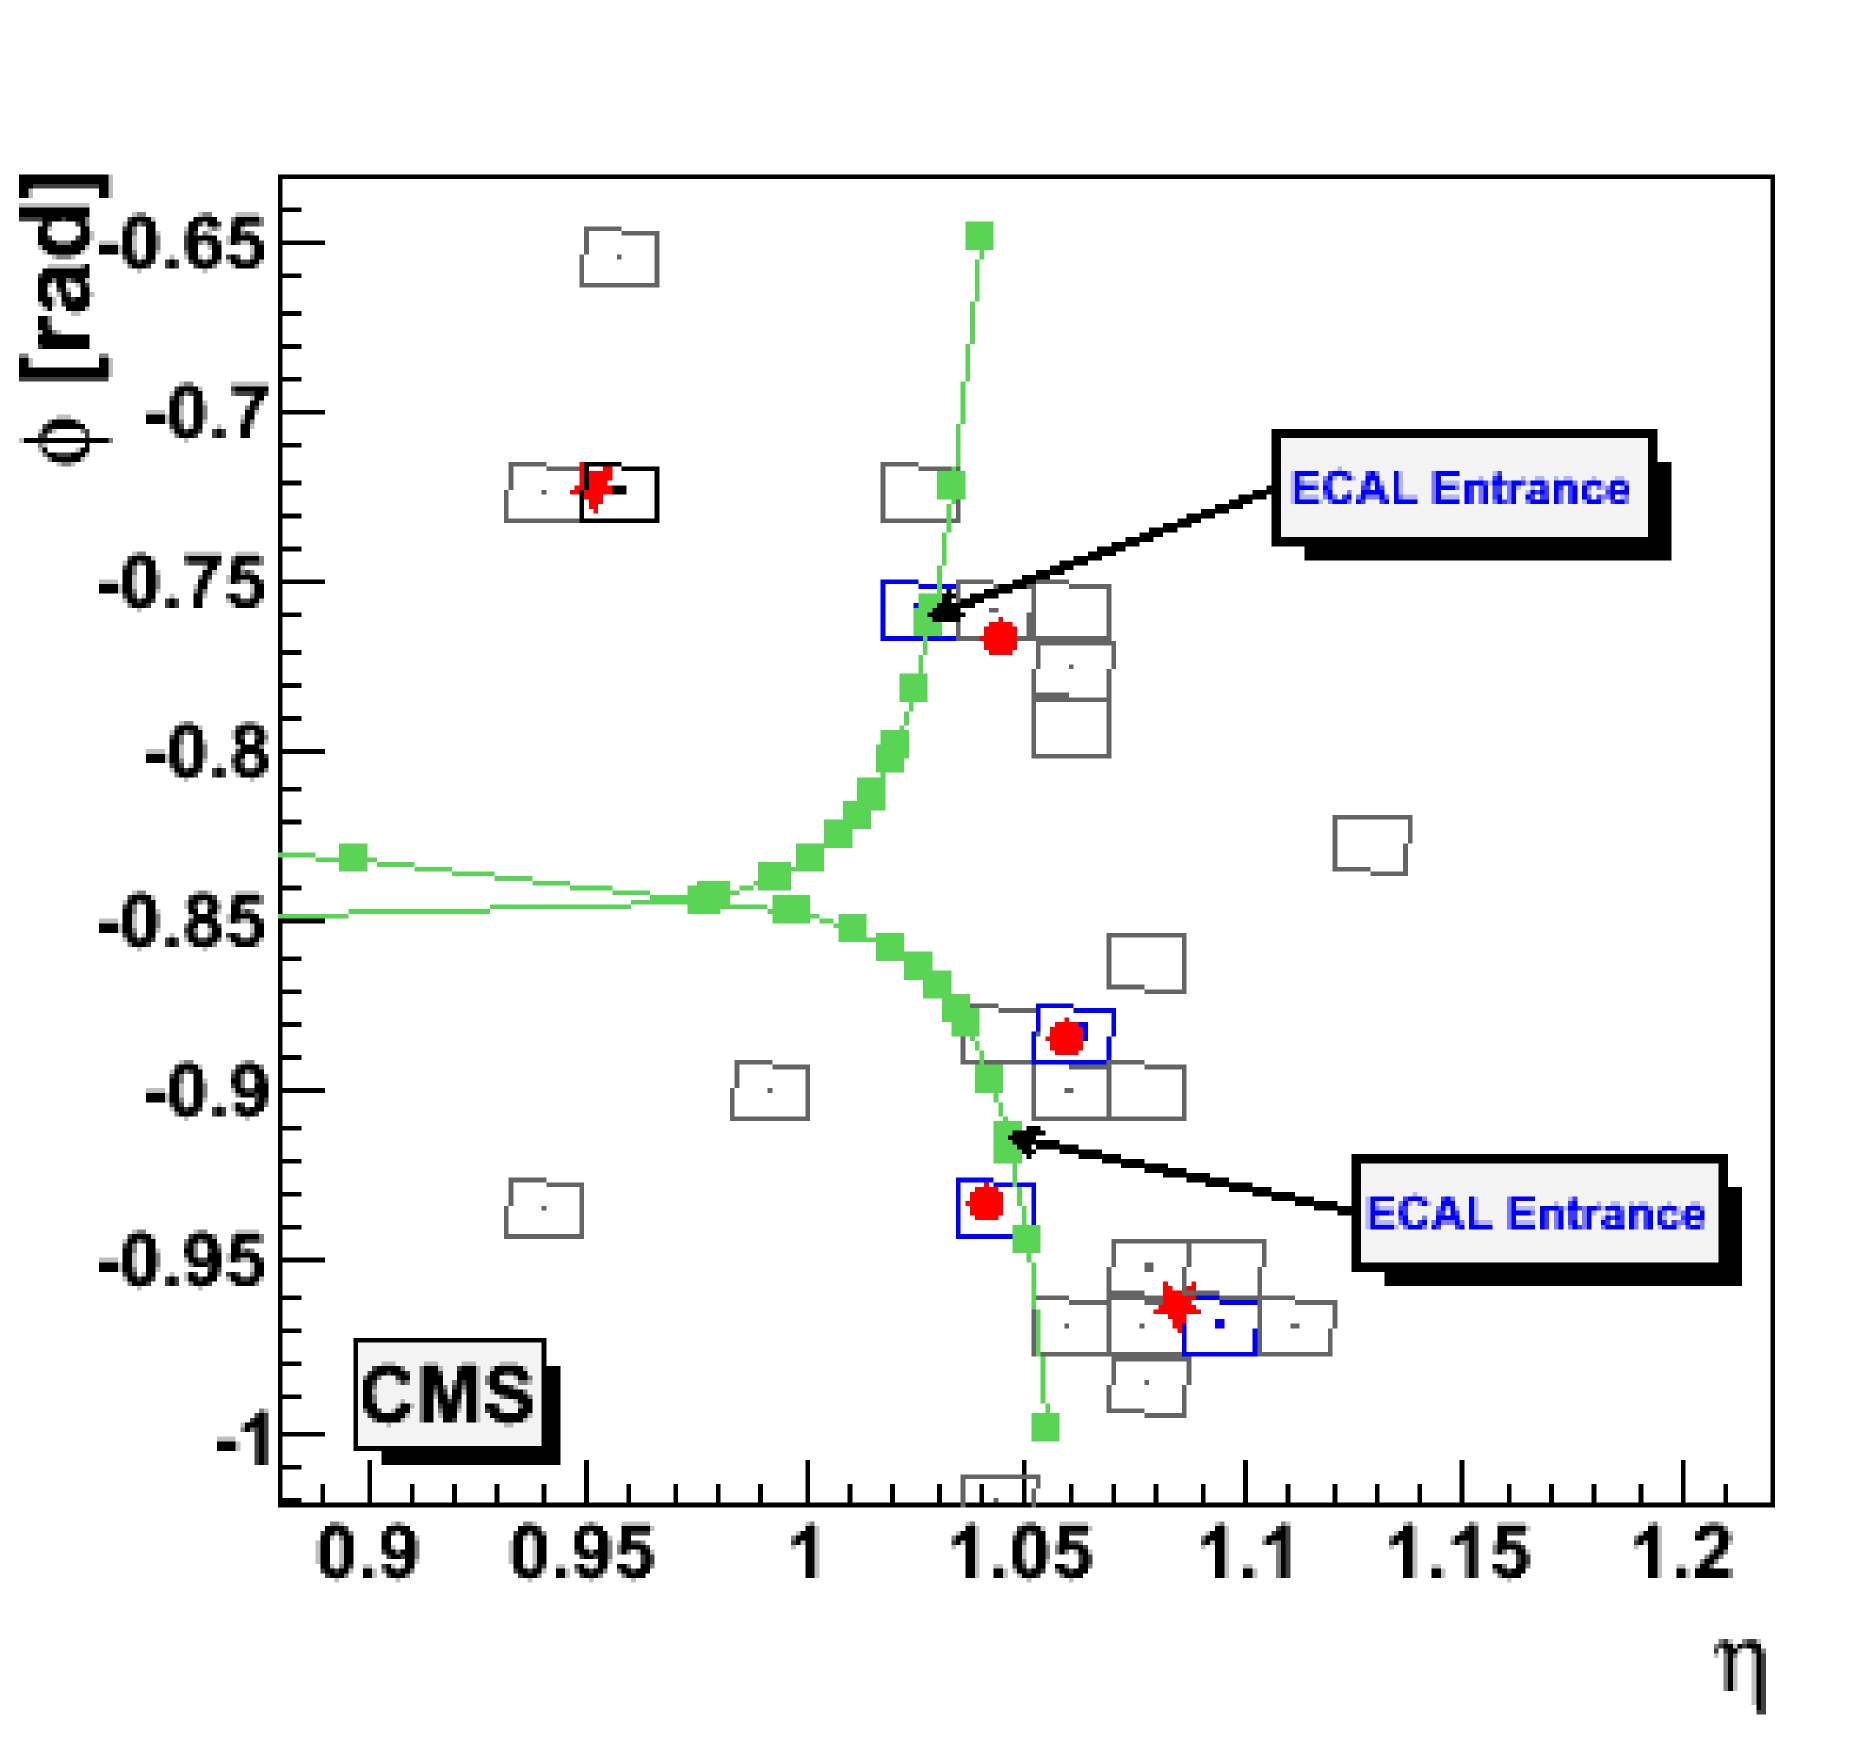
\includegraphics[width=0.45\textwidth]{chapitre3/figs/pf_links_ecal.png}}\hfill
  \subcaptionbox{HCAL\label{fig:pf_links_hcal}}[0.45\textwidth]{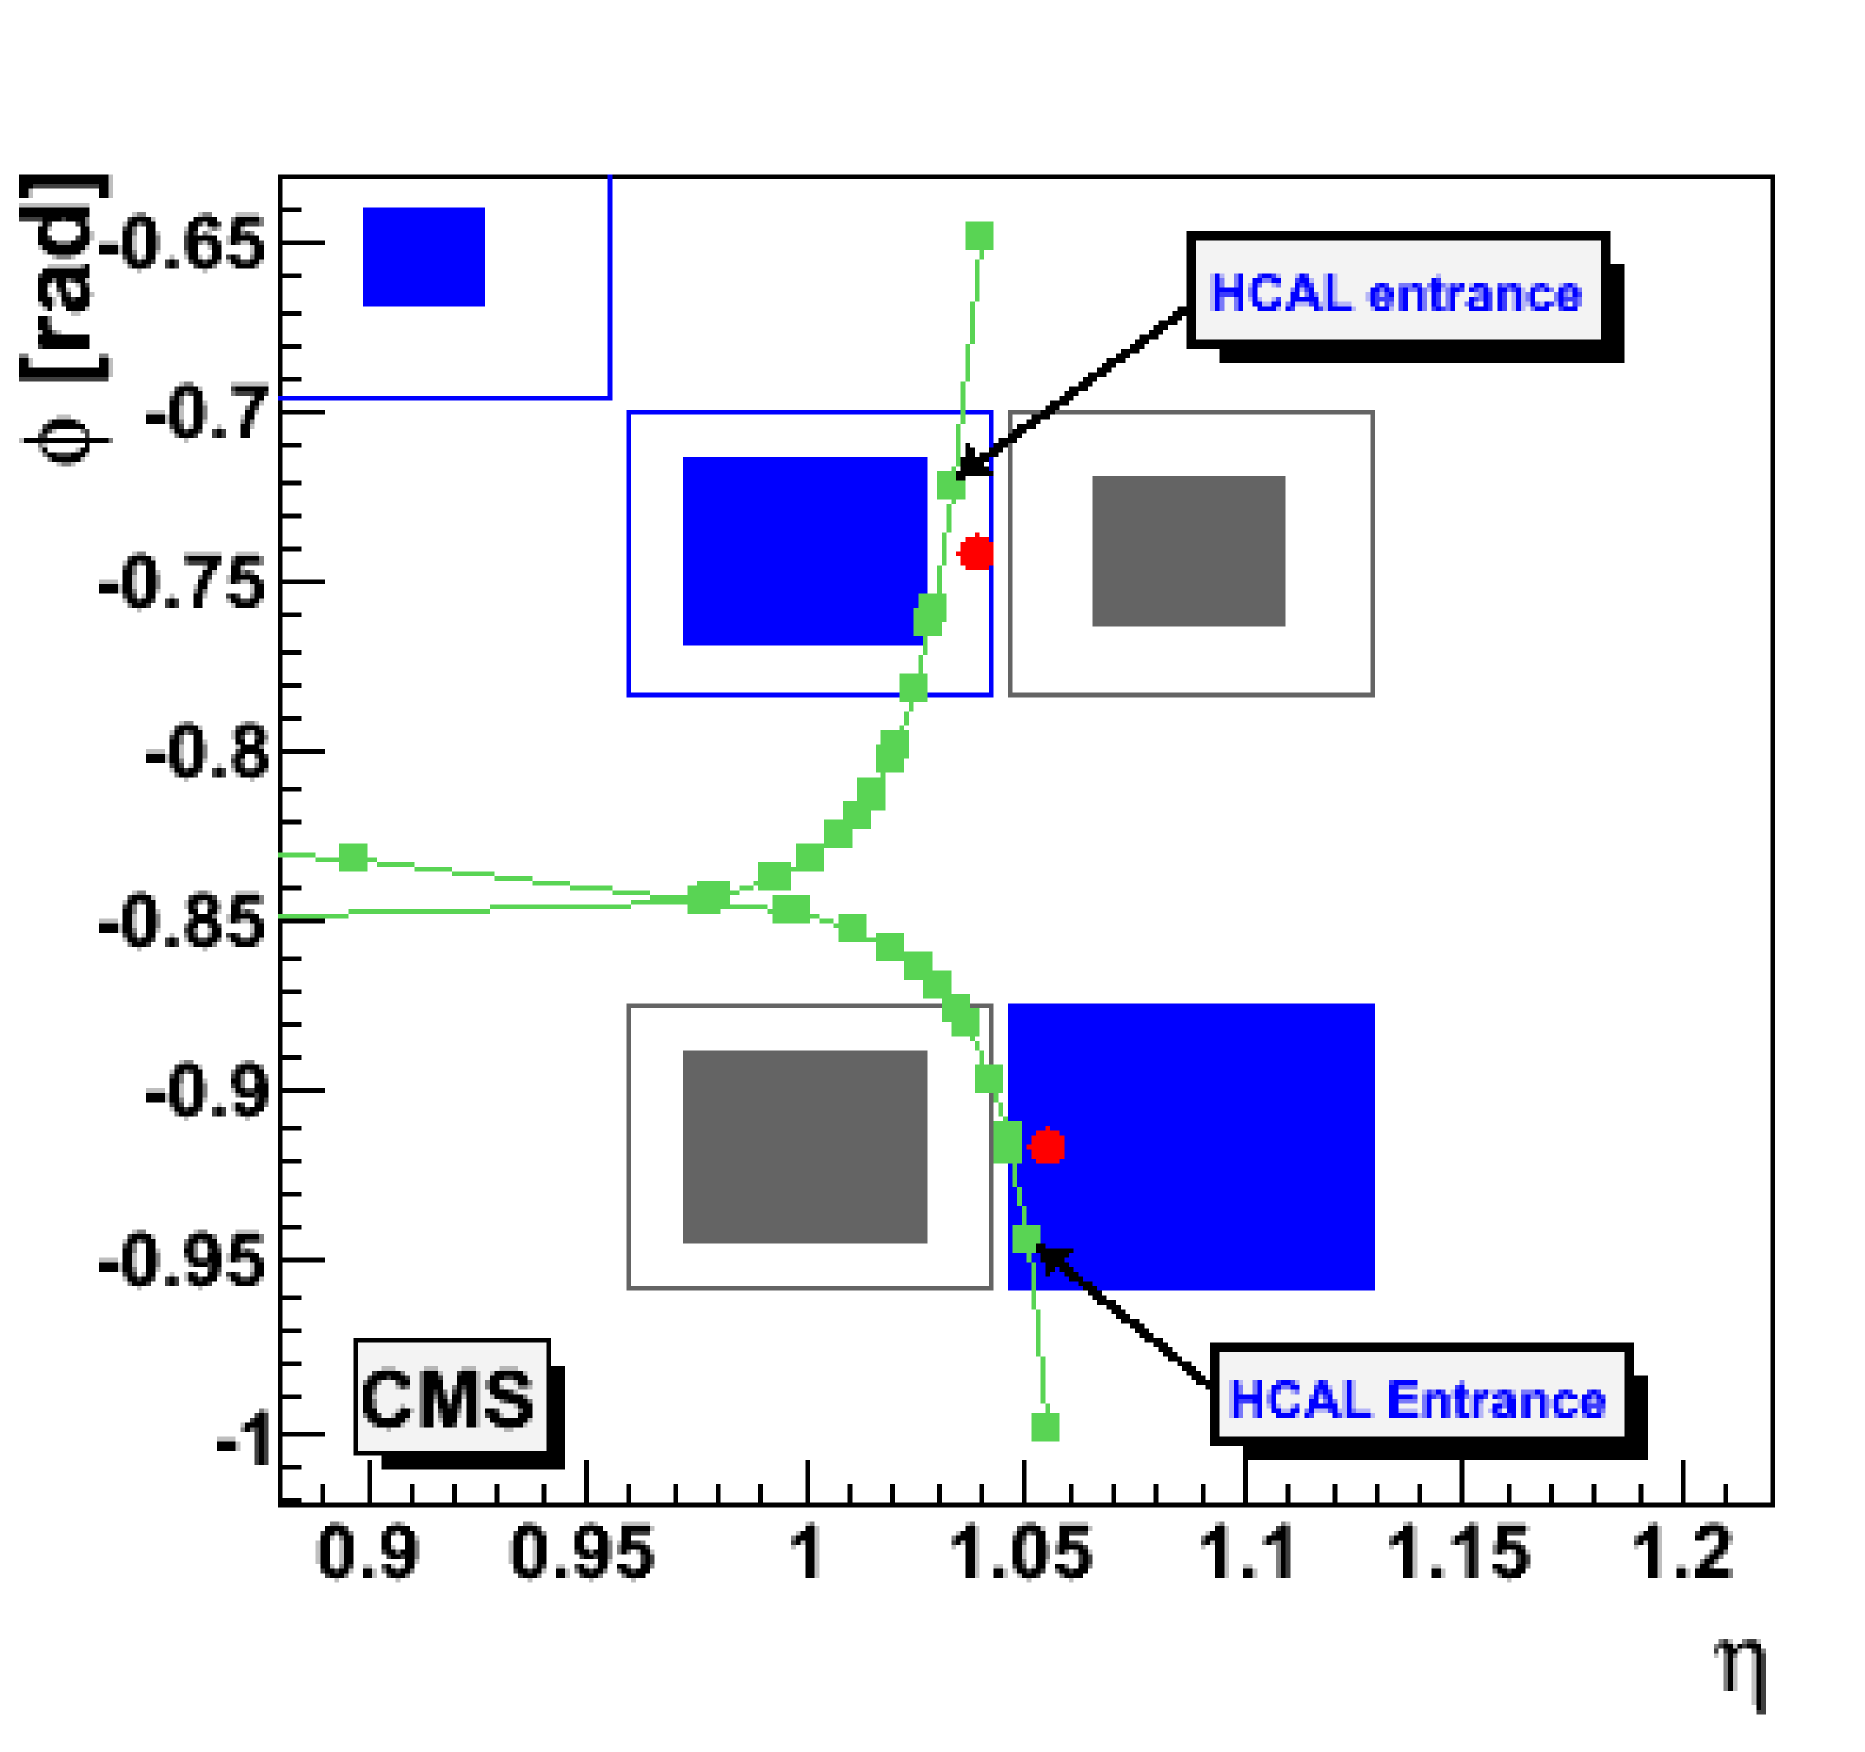
\includegraphics[width=0.45\textwidth]{chapitre3/figs/pf_links_hcal.png}}
  \caption{Connexion entre les traces et les agrégats calorimétriques. Les traces (les lignes vertes avec marqueurs carrés) sont liées avec un ou deux agrégats dans le ECAL (\subref{fig:pf_links_ecal}) et un agrégat dans le HCAL (\subref{fig:pf_links_hcal}). Chaque carré gris représente une cellule calorimétrique. Les ronds rouges représente les agrégats liés à une trace, alors que les étoiles rouges sont les agrégats non liés.}
  \label{fig:pf_links}
\end{figure}

Afin de collecter l'énergie perdue par les électrons par rayonnement Bremsstrahlung, des trajectoires tangentes à la trajectoire principale sont extrapolées dans le ECAL. Un agrégat est lié à la trace principale comme candidat photon Bremsstrahlung si la trajectoire extrapolée passe dans la zone de l'agrégat, comme défini juste avant.

\paragraph{Les liens ECAL – HCAL}

De façon similaire, un lien entre les deux calorimètres est créé lorsque la position de l'agrégat formé dans le calorimètre électromagnétique est contenu dans la zone limitée par l'agrégat formé dans le calorimètre hadronique. L'enveloppe des agrégats peut ici aussi être agrandie d'une unité de chaque côté. La distance du lien est donné par $\Delta R$. %dans le plan ($\eta$, $\phi$).

\paragraph{Les liens trajectographe – détecteur à muons} \label{sec:pf_link_mu}

Le spectromètre à muons reconstruit aussi des traces. Un lien est fait (qu'on appelle muon global) avec les traces du trajectographe lorsque l'ajustement entre les deux traces donne un $\chi^2$ acceptable. Si une trace dans le détecteur à muons peut être associée à plusieurs traces dans le trajectographe, le lien est fait entre les deux traces qui donnent le plus petit $\chi^2$. Pour ce type de lien, la distance du lien est donné par le $\chi^2$.

\subsection{L'identification des particules}

Après application de l'algorithme de liaison (voir \cref{sec:pf_links}), on dispose d'une liste de blocs, composés chacun d'environ 2-3 éléments (traces ou agrégats calorimétriques). Il reste maintenant à identifier chaque bloc en tant que particule. Cette identification conduira à la création d'une liste de particules, donnant une description globale de l'événement.

\subsubsection{Reconstruction des muons} \label{sec:muon_reco}

Les premières particules à être reconstruites sont les muons \citep{cms_muons_reco}, avant même le début de la reconstruction de l'événement grâce au \emph{particle-flow}. Les muons laissant des traces à la fois dans le trajectographe et dans le spectromètre à muons, deux types de reconstructions sont utilisées :

\begin{description}
    \item[Reconstruction des muons globaux] Pour chaque trace dans le spectromètre à muons, on cherche par extrapolation une trace correspondante dans le trajectographe, afin de déterminer une trace globale grâce à une interpolation des deux trajectoires. Cette technique est similaire à celle utilisée dans l'algorithme de lien trajectoire -- détecteur à muons présenté \cref{sec:pf_link_mu}. A haute impulsion transverse ($\pt \gtrsim \SI{200}{\GeV}$), cette méthode permet d'améliorer la résolution de l'impulsion comparé à l'utilisation de la trace du trajectographe uniquement.
    \item[Reconstruction des \emph{tracker} muons] On ne considère ici que les traces présentes dans le trajectographe comme possibles candidats muons. Ces traces sont extrapolées jusqu'au détecteur à muons, en prenant en compte les pertes d'énergie et l'incertitude due aux multiples diffusions. Si au moins un segment\footnote{Un segment correspond à une petite trace dans le spectromètre à muons, composée de quelques \emph{hits} de DT ou CSC} dans le spectromètre coïncide avec la trajectoire extrapolée, la trace est identifiée comme un muon. Pour les muons de faible impulsion ($\pt \lesssim
 \SI{5}{\GeV}$), cette approche est plus performante que la reconstruction des muons globaux, puisqu'il est nécessaire d'avoir un seul segment qui coïncide, au lieu de plusieurs pour l'autre méthode.
\end{description}

La majorité des muons sont reconstruits comme muons globaux ou \emph{tracker} muons, voire comme les deux. Cependant, pour environ \SI{1}{\%} des muons, aucune trace n'est trouvée dans le trajectographe. On classe donc ces muons dans une troisième catégorie, les muons \emph{standalone}.

\medskip

\begin{figure}[tbp]
    \centering
    \subcaptionbox{\label{fig:dimu_jpsi}}[0.49\textwidth]{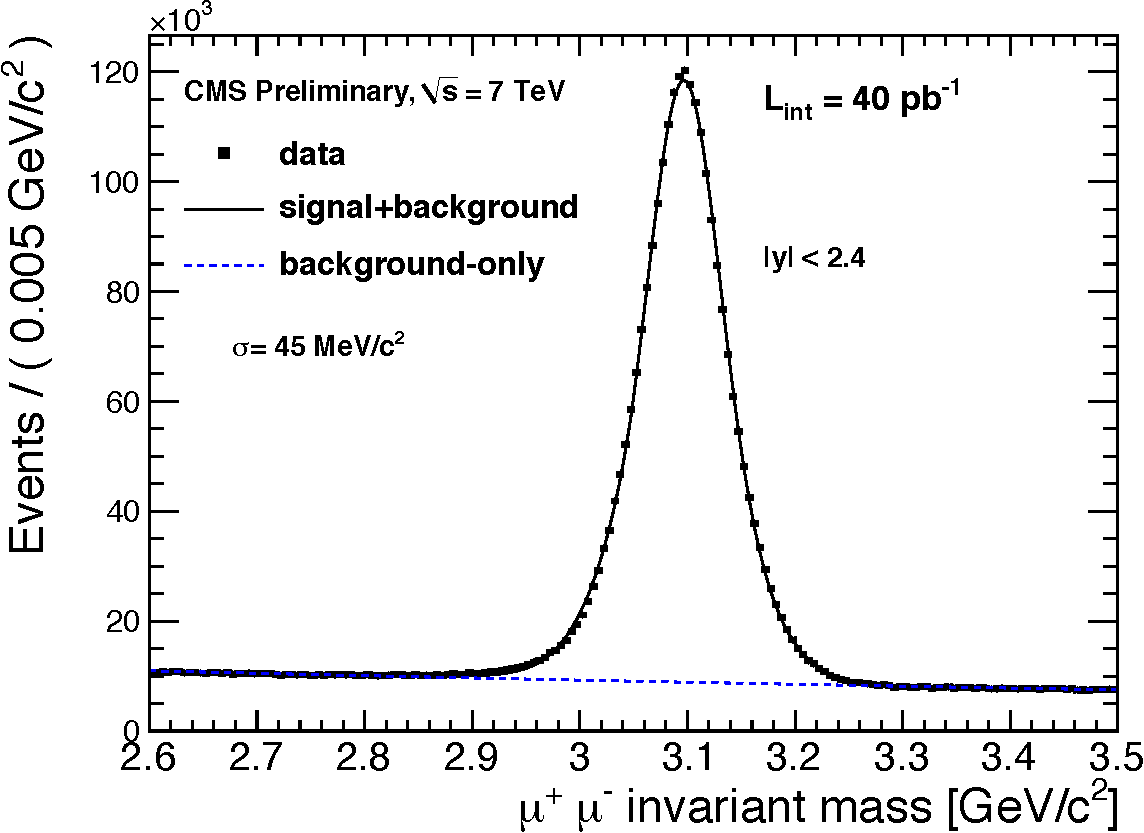
\includegraphics[width=0.49\textwidth]{chapitre3/figs/JPsi40pb-1.pdf}} \hfill
    \subcaptionbox{\label{fig:dimu_mass}}[0.49\textwidth]{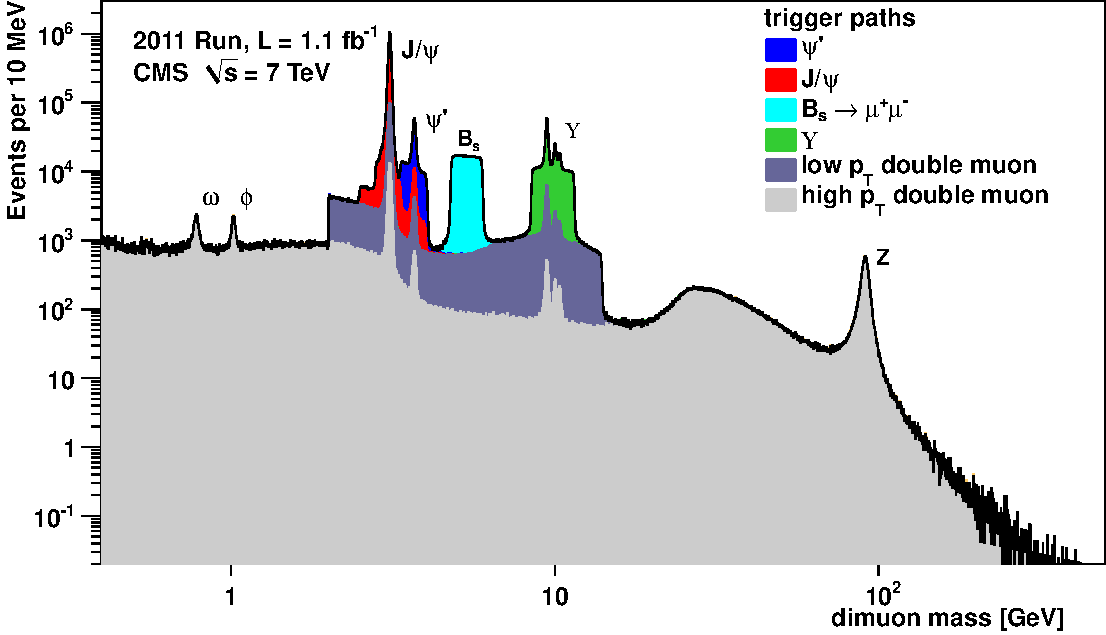
\includegraphics[width=0.49\textwidth]{chapitre3/figs/mass_dimu.pdf}}
    \caption{(\subref{fig:dimu_jpsi}) Comparaison entre la simulation et les données pour des événements $\PJpsi \rightarrow \Pmuon \APmuon$, reconstruit à l'aide des données 2010. La résolution sur la reconstruction du pic de masse du \PJpsi est de $\SI{45}{\MeV}$. (\subref{fig:dimu_mass}) Spectre de masse invariante di-muons reconstruit à l'aide des données 2011. L'excellente résolution permet même de reconstruire les résonances $\omega$ et $\phi$.}
    \label{fig:dimu_mass_spectrum}
\end{figure}

On regroupe ensuite les trois catégories de muons dans une liste de candidats muons. Les candidats muons globaux et \emph{tracker} muons qui partagent la même trace du trajectographe sont fusionnés en un seul candidat.

Afin d'identifier les muons \emph{particle-flow}, une sélection est effectuée sur les candidats muons reconstruits avec l'algorithme standard. On dénombre trois sélections différentes : "isolé", "\emph{pf-tight}" et "\emph{pf-loose}". Les muons sont considérés isolés si, dans un cône de taille $R = \num{0.3}$ centré sur le muon, la somme du \pt des traces et des agrégats calorimétriques est inférieure à \SI{10}{\%} de l'impulsion du muon. Dans ce cas, l'effet du \emph{particle-flow} est limité puisque l'environnement immédiat autour du muon est propre. Par conséquent, une grande efficacité est obtenue en appliquant une sélection peu contraignante : les muons doivent seulement être des muons globaux.

Une fois les muons isolés traités, les sélections \emph{pf-loose} et \emph{pf-tight} sont appliquées aux muons restants. Ces deux sélections sont optimisées pour identifier les muons au sein des jets. La sélection \emph{pf-tight} demande un certain nombre de \emph{hits} dans les traces du spectromètre à muons. Il faut de plus que les dépôts d'énergies dans les calorimètres soient compatibles avec ceux obtenus par des simulations. La sélection \emph{pf-loose} relâche la contrainte sur le nombre de \emph{hits}, et supprime la contrainte sur les dépôts d'énergies.

Pour chaque muon reconstruit, on enlève les blocs \emph{particle-flow} correspondants de la liste des blocs disponibles, et on procède ensuite à la reconstruction des électrons. On présente \cref{fig:dimu_mass_spectrum} les performances de reconstruction des muons à l'aide du \pu. La résolution obtenue sur des événements $\PJpsi \rightarrow \Pmuon \APmuon$ est mesurée à $\sigma = \SI{45}{\MeV}$ (\cref{fig:dimu_jpsi}). On peut aussi voir \cref{fig:dimu_mass} le spectre de masse invariante di-muons reconstruit à l'aide des données 2011. L'excellente performance de la reconstruction permet de reconstruire les résonances di-muons de 1 à \SI{100}{\GeV}.

\subsubsection{Reconstruction des électrons}

L'algorithme de reconstruction des traces de CMS (voir \cref{sec:tracks_reconstruction}) est optimisé pour reconstruire les traces des muons. Les électrons étant beaucoup plus léger que les muons, la radiation Bremsstrahlung est amplifiée par un facteur $\left( \sfrac{m_\mu}{m_e} \right)^4 \simeq \num{1.83e9}$, ce qui met en défaut l'algorithme de reconstruction des traces. En effet, la trajectoire des électrons peut changer brusquement lors de l'émission d'un photon Bremsstrahlung, et l'algorithme de reconstruction n'arrive plus à suivre la trajectoire abrupte de l'électron. En cas d'émission d'un photon de basse énergie, l'algorithme peut arriver à reconstruire quand même la trajectoire de l'électron, mais au prix d'une grande incertitude et d'un $\chi^2$ grand.

Un algorithme dédié a été développé par CMS pour contrer ces problèmes \citep{pf,cms_pf_leptons,cms_pf_electrons}. La trajectoire de l'électron est redéfinie, en modélisant le rayonnement Bremsstrahlung par une somme de gaussienne (algorithme GSF, pour \emph{Gaussian Sum Filter}. Le nombre de paramètres libres étant important (plus d'une dizaine), l'algorithme est capable de suivre les brusques changements de trajectoires, et procure ainsi une bien meilleure estimation de l'impulsion des électrons. En contre-partie, cet algorithme est très gourmand en ressource (environ \SI{200}{\ms} par trace), et ne peut donc être utilisé que sur un nombre réduit de traces. Il est alors nécessaire d'effectuer une pré-sélection dans les traces existantes afin d'extraire celles qui ont le plus de chance d'être produites par un électron.

\begin{figure}[tbp]
    \centering
    \subcaptionbox{\label{fig:bdt_electron}}[0.5\textwidth]{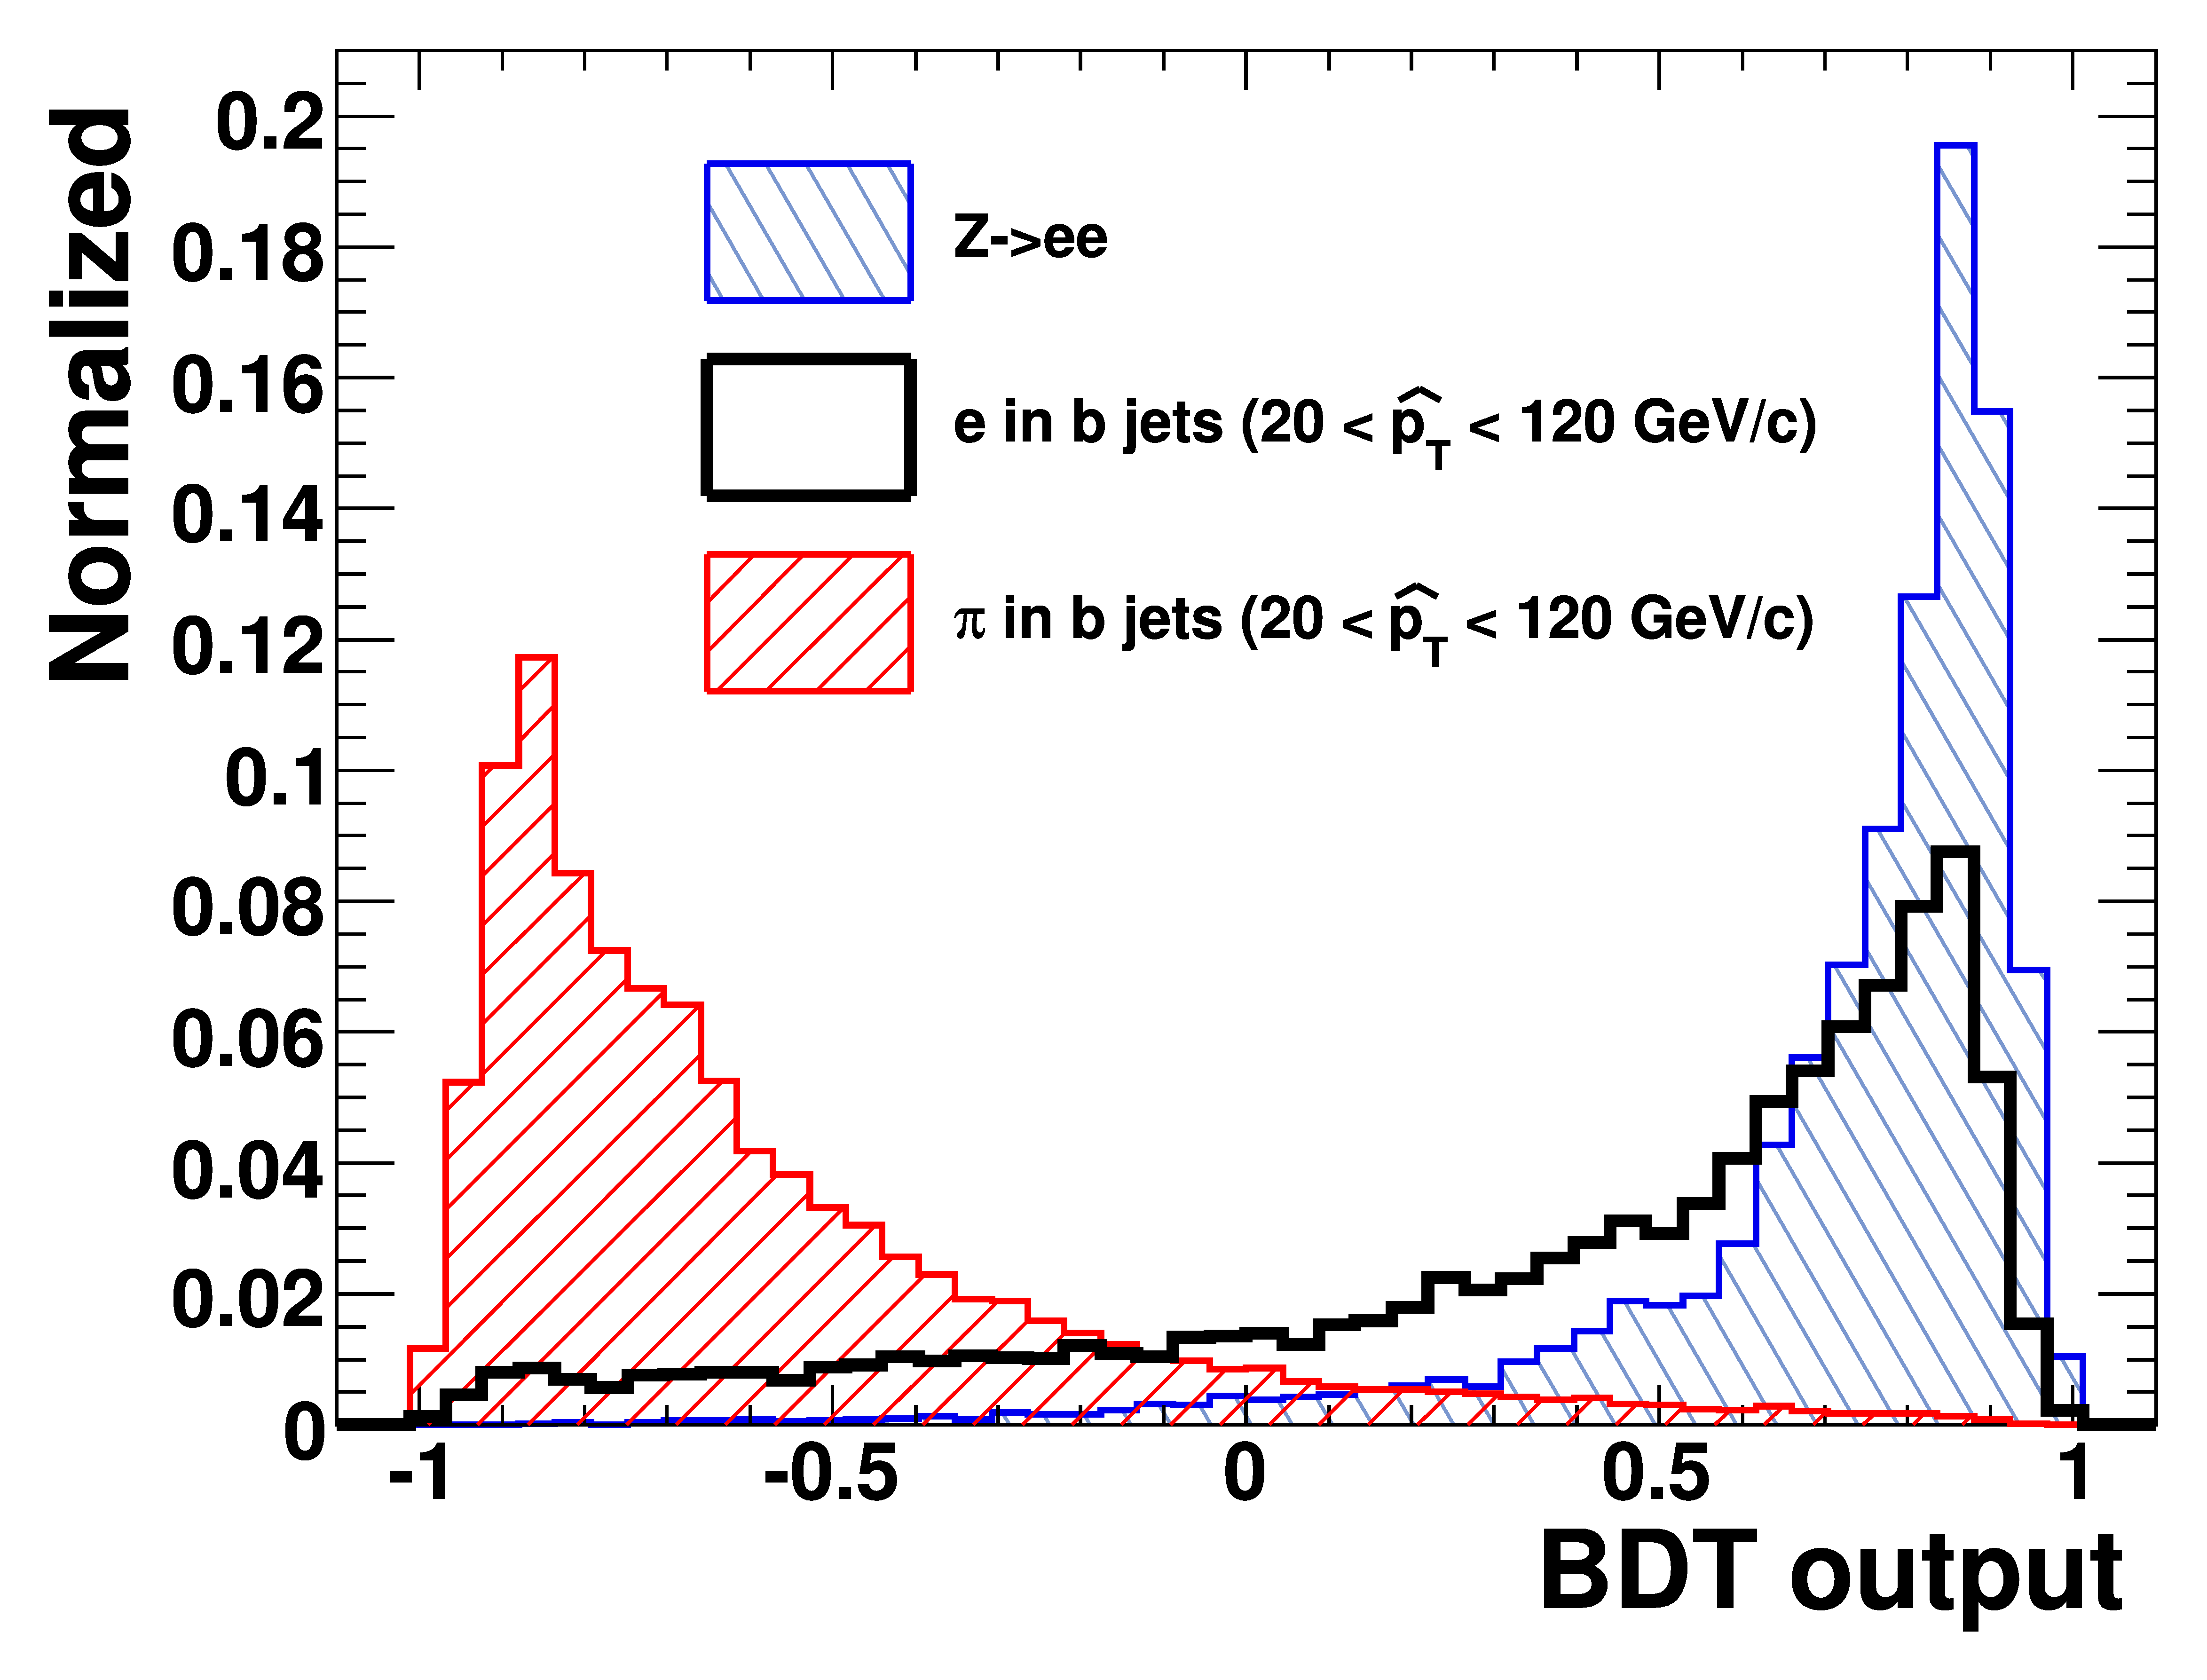
\includegraphics[width=0.5\textwidth]{chapitre3/figs/bdt_electron.pdf}} \hfill
    \subcaptionbox{\label{fig:jspi_ee}}[0.45\textwidth]{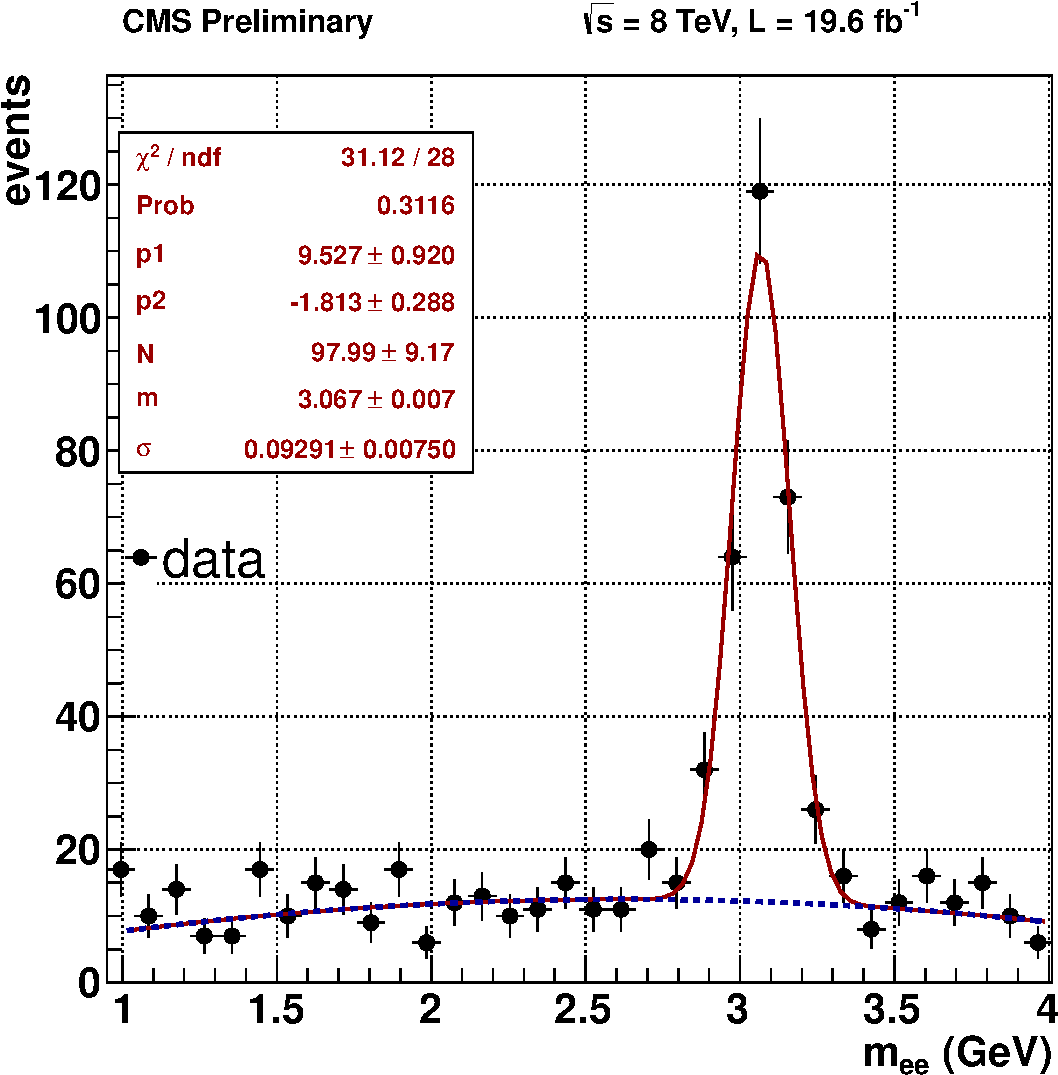
\includegraphics[width=0.45\textwidth]{chapitre3/figs/jspi_ee.pdf}}
    \caption{(\subref{fig:bdt_electron}) Sortie de l'algorithme de pré-sélection des électrons, pour des électrons isolés (bleu), des électrons dans des jets de $b$ (noir) et pour des pions dans des jets de $b$ \citep{pf}. (\subref{fig:jspi_ee}) Masse invariante di-électrons sur les données 2012 pour des événements $\PJpsi \rightarrow \Pelectron \Ppositron$ \citep{cms_electron_perf}.}
    \label{fig:electron_perf}
\end{figure}

La pré-sélection des électrons exploite les caractéristiques des traces. Lorsque la radiation Bremsstrahlung est négligeable, l'algorithme classique reconstruit une trace et on trouve un bloc \emph{particle-flow} associé. Si le rapport $E/p$ est proche de l'unité, la trace est sélectionnée. Lorsque le rayonnement Bremsstrahlung n'est pas négligeable, deux effets sont possibles :
\begin{itemize}
    \item L'algorithme de reconnaissance de traces échoue lors d'un changement abrupt de trajectoire. La trace résultante contient alors un petit nombre de \emph{hits}.
    \item L'algorithme de reconnaissance de traces reconstruit une trace, mais le $\chi^2$ associé est grand.
\end{itemize}

Une sélection est appliquée en utilisant le nombre de \emph{hits} et le $\chi^2$, puis une interpolation GSF (avec seulement 5 paramètres libres, donc moins contraignante) est effectuée si la trace passe la sélection. Le $\chi^2$ de cette interpolation ($\chi^2_{GSF}$), le rapport $\chi^2_{KF} / \chi^2_{GSF}$, le nombre de \emph{hits} ainsi que le facteur de qualité du lien ECAL -- trace sont utilisés en entrée d'un algorithme d'arbres de décision boosté. La sortie de cet algorithme est présentée \cref{fig:bdt_electron}. On peut voir l'excellente discrimination entre les électrons isolés et les pions, et la bonne séparation entre les électrons non isolés et les pions. Les performances de reconstruction des électrons sont évaluées sur des événements \PJpsi $\rightarrow \Pelectron \APelectron$ (\cref{fig:jspi_ee}). On obtient une résolution de reconstruction $\sigma = \SI{93}{\MeV}$.

On considère le candidat comme un électron si la sortie de l'algorithme est supérieure à \num{-0.1} \citep{cms_pf_electrons}. Dans ce cas, les blocs \emph{particle-flow} sont retirés de la liste des blocs disponibles.

\subsubsection{Reconstruction des hadrons et des photons}

A ce stade, il ne reste plus que les blocs \emph{particle-flow} correspondant aux hadrons (chargés ou neutres), ainsi qu'aux photons. Avant d'entamer la reconstruction, il convient de simplifier un peu les liens créés par l'algorithme de liaison. Si une trace est liée à plusieurs agrégats dans le HCAL, seule le lien ayant la plus petite distance ($\Delta R$, voir \cref{sec:pf_links}) est gardée. On procède de façon identique pour les liens dans le ECAL.

Dans de très rares cas, l'énergie des agrégats calorimétriques liés à une trace peut être très inférieure à l'impulsion de celle-ci. Si cette différence est supérieure à $3\sigma$, cela est probablement le signe de la présence d'un muon, ou d'une fausse trace. Un algorithme spécialisé, basé sur le même principe que celui servant à reconstruire les muons, mais avec des contraintes relâchées, permet d'identifier ces muons. S'il s'avère qu'aucun muon n'est présent, la trace est considérée comme fausse et est supprimée des blocs \emph{particle-flow}. Moins de \SI{0.3}{‰} des traces sont concernées par cette procédure.

Chaque trace restante donne lieu à la création de hadrons chargés \emph{particle-flow}, dont l'impulsion et l'énergie est mesurée directement depuis la trace, selon l'hypothèse d'un pion chargé. Deux cas sont possibles :
\begin{itemize}
    \item L'énergie des agrégats calorimétriques liés à cette trace est compatible avec l'impulsion mesurée par la trace (dans les incertitudes). L'impulsion du hadron chargé est alors améliorée en combinant les informations de la trace et des agrégats calorimétriques, grâce à une moyenne pondérée. Cette combinaison est surtout intéressante à très haute énergie / très haut \aeta, où les paramètres des traces sont mesurés avec une grande incertitude.
    \item L'énergie des agrégats calorimétriques est plus grande que l'impulsion de la trace liée. C'est le cas si des photons ou des hadrons neutres, ne laissant pas de traces dans le trajectographe, ont déposés leur énergie au même endroit. Il faut donc réussir à correctement associer l'énergie avec les bonnes particules.

    \smallskip

    Si l'excès d'énergie ($E_\text{agrégats} - p_\text{trace}$) est supérieur à l'énergie déposée dans le ECAL ($E_E$), deux particules sont reconstruites : on assigne l'énergie du ECAL à un photon \emph{particle-flow}, et le restant de l'excès ($E_\text{HCAL} - p_\text{trace}$) à un hadron neutre \emph{particle-flow}. Dans le cas contraire, seul un photon \emph{particle-flow} est reconstruit avec l'excès d'énergie. La priorité donnée aux photons sur les hadrons neutres dans le ECAL est justifiée par l'observation que seul environ \SI{3}{\%} de l'énergie des hadrons neutres est déposée dans le calorimètre électromagnétique.
\end{itemize}

Enfin, les blocs \emph{particle-flow} restant n'ont aucune trace liée. On reconstruit avec les agrégats dans le ECAL les photons \emph{particle-flow}, et avec ceux dans le HCAL les hadrons neutres \emph{particle-flow}.

\begin{figure}[tbp]
    \centering
    \subcaptionbox{\label{fig:mgg}}[0.55\textwidth]{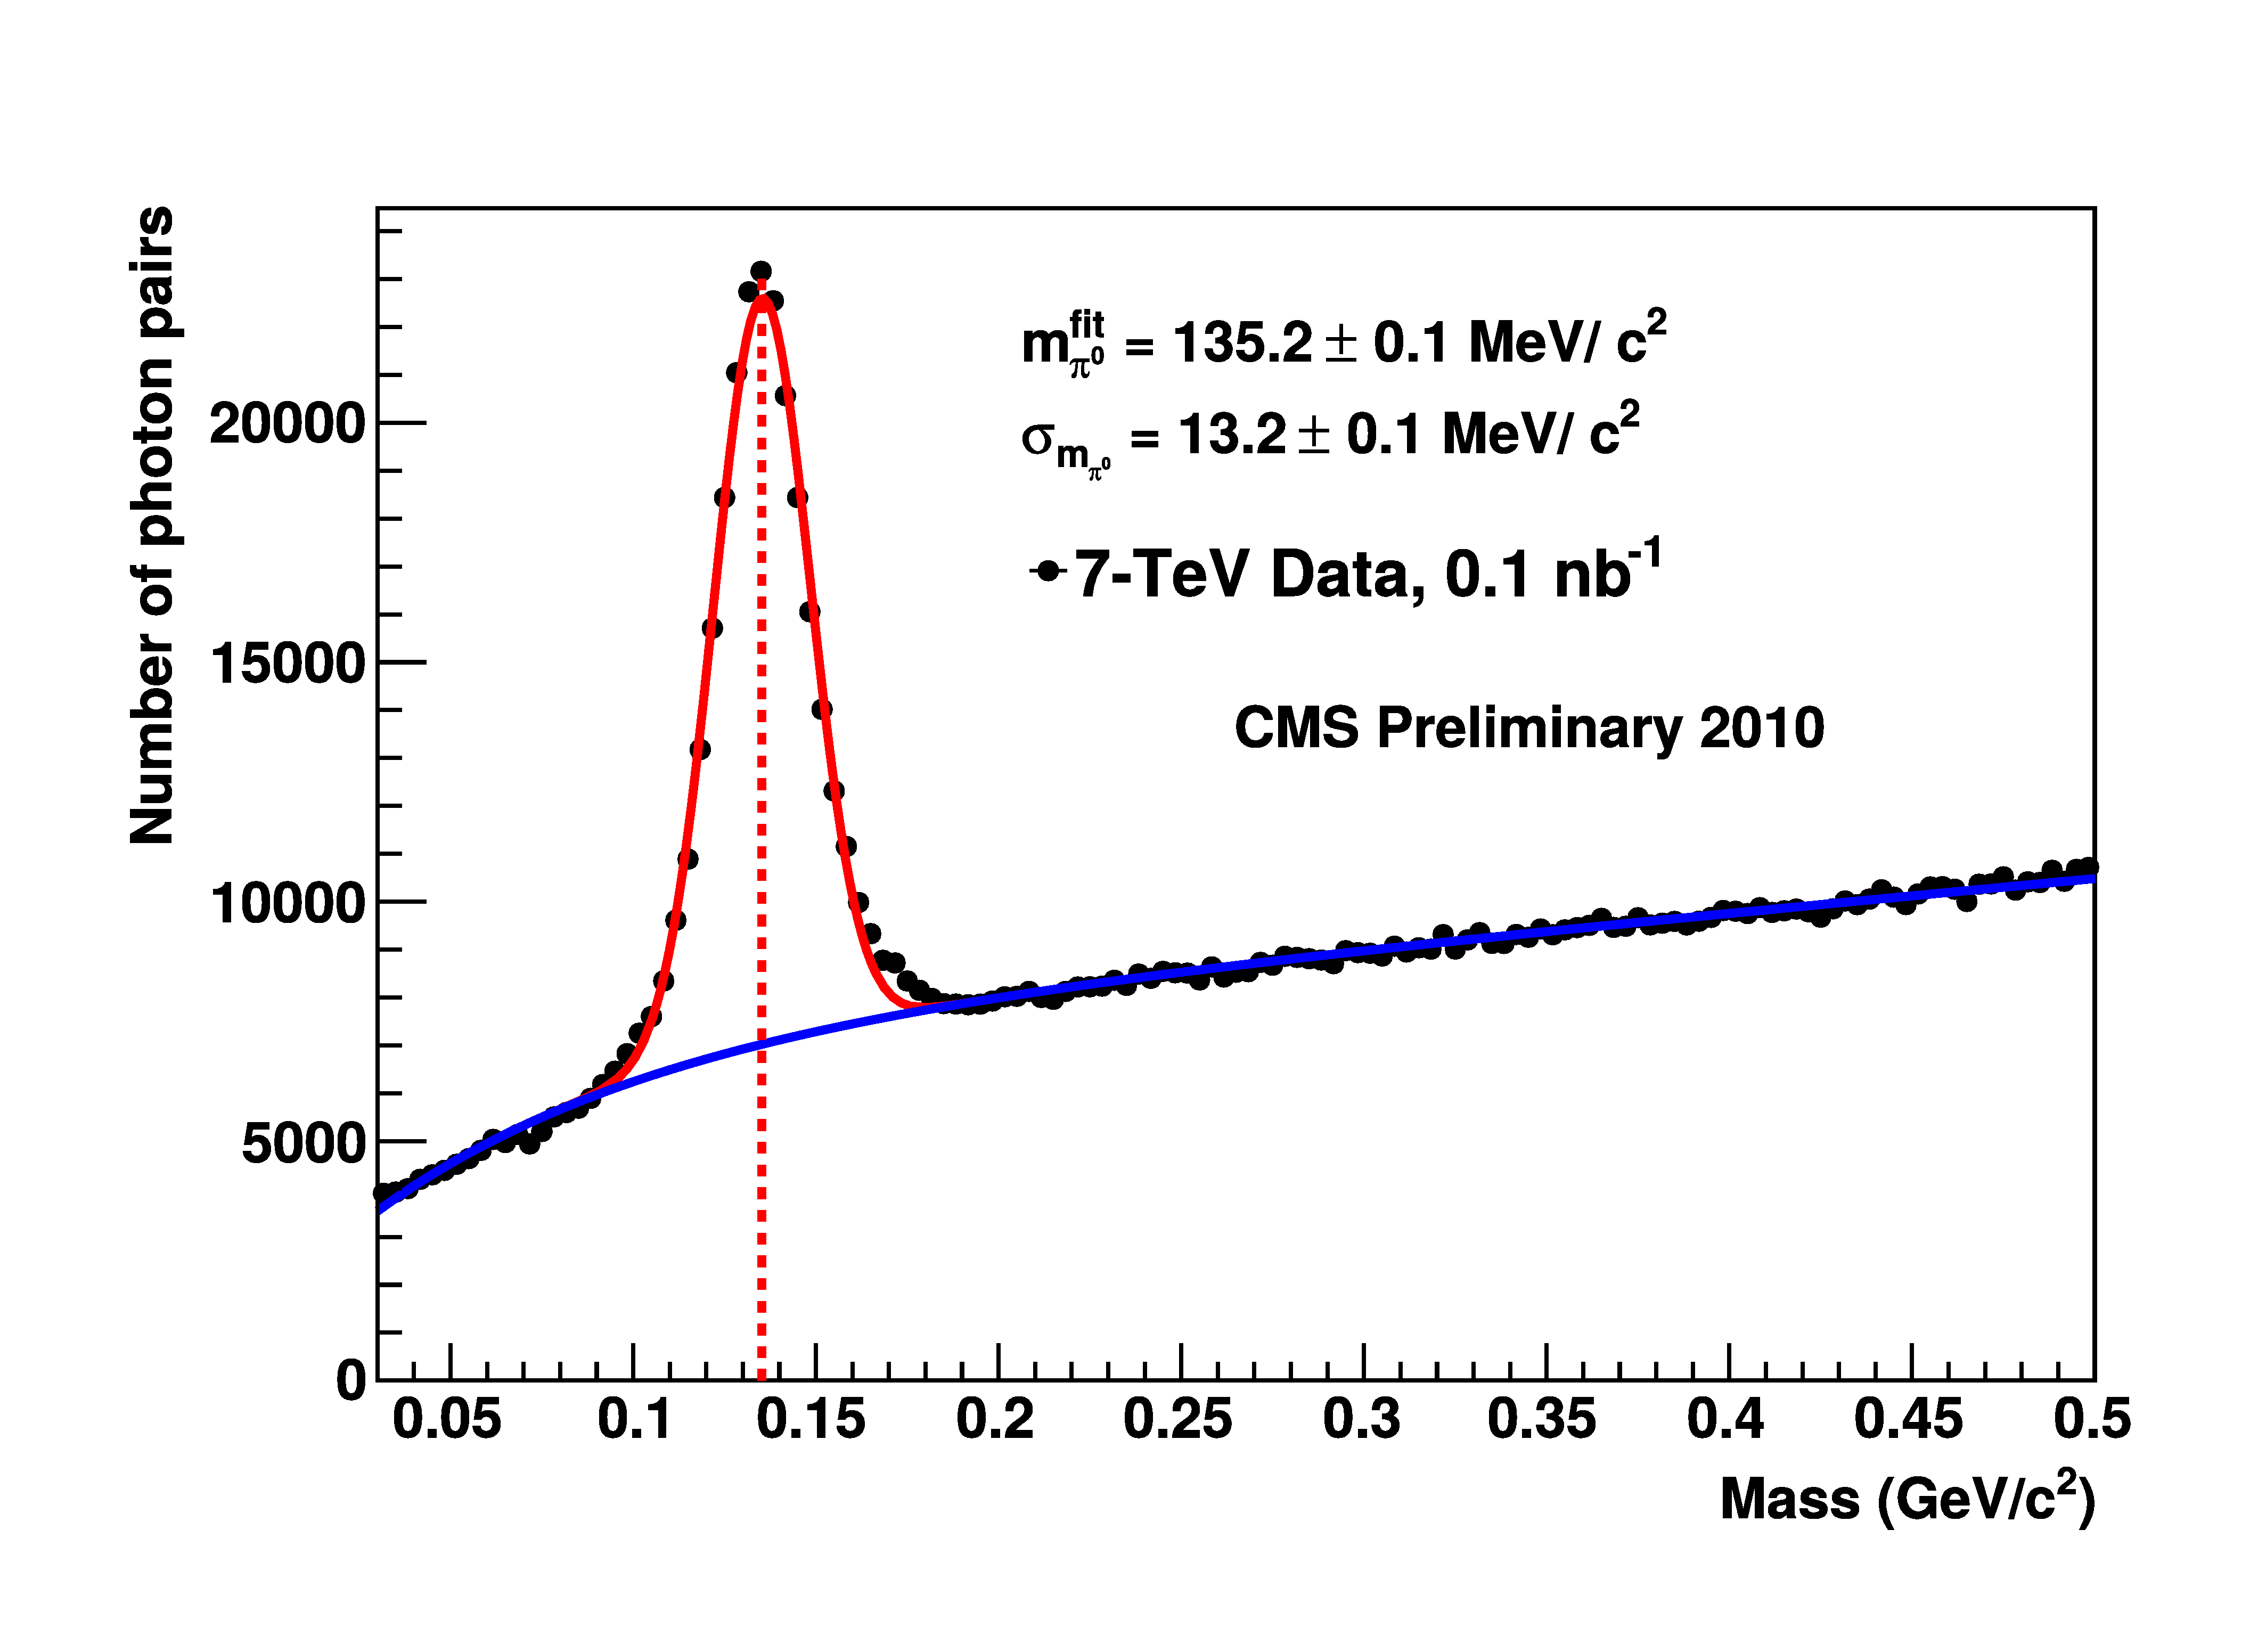
\includegraphics[width=0.55\textwidth]{chapitre3/figs/pf_photons.pdf}} \hfill
    \subcaptionbox{\label{fig:gamma_eff}}[0.44\textwidth]{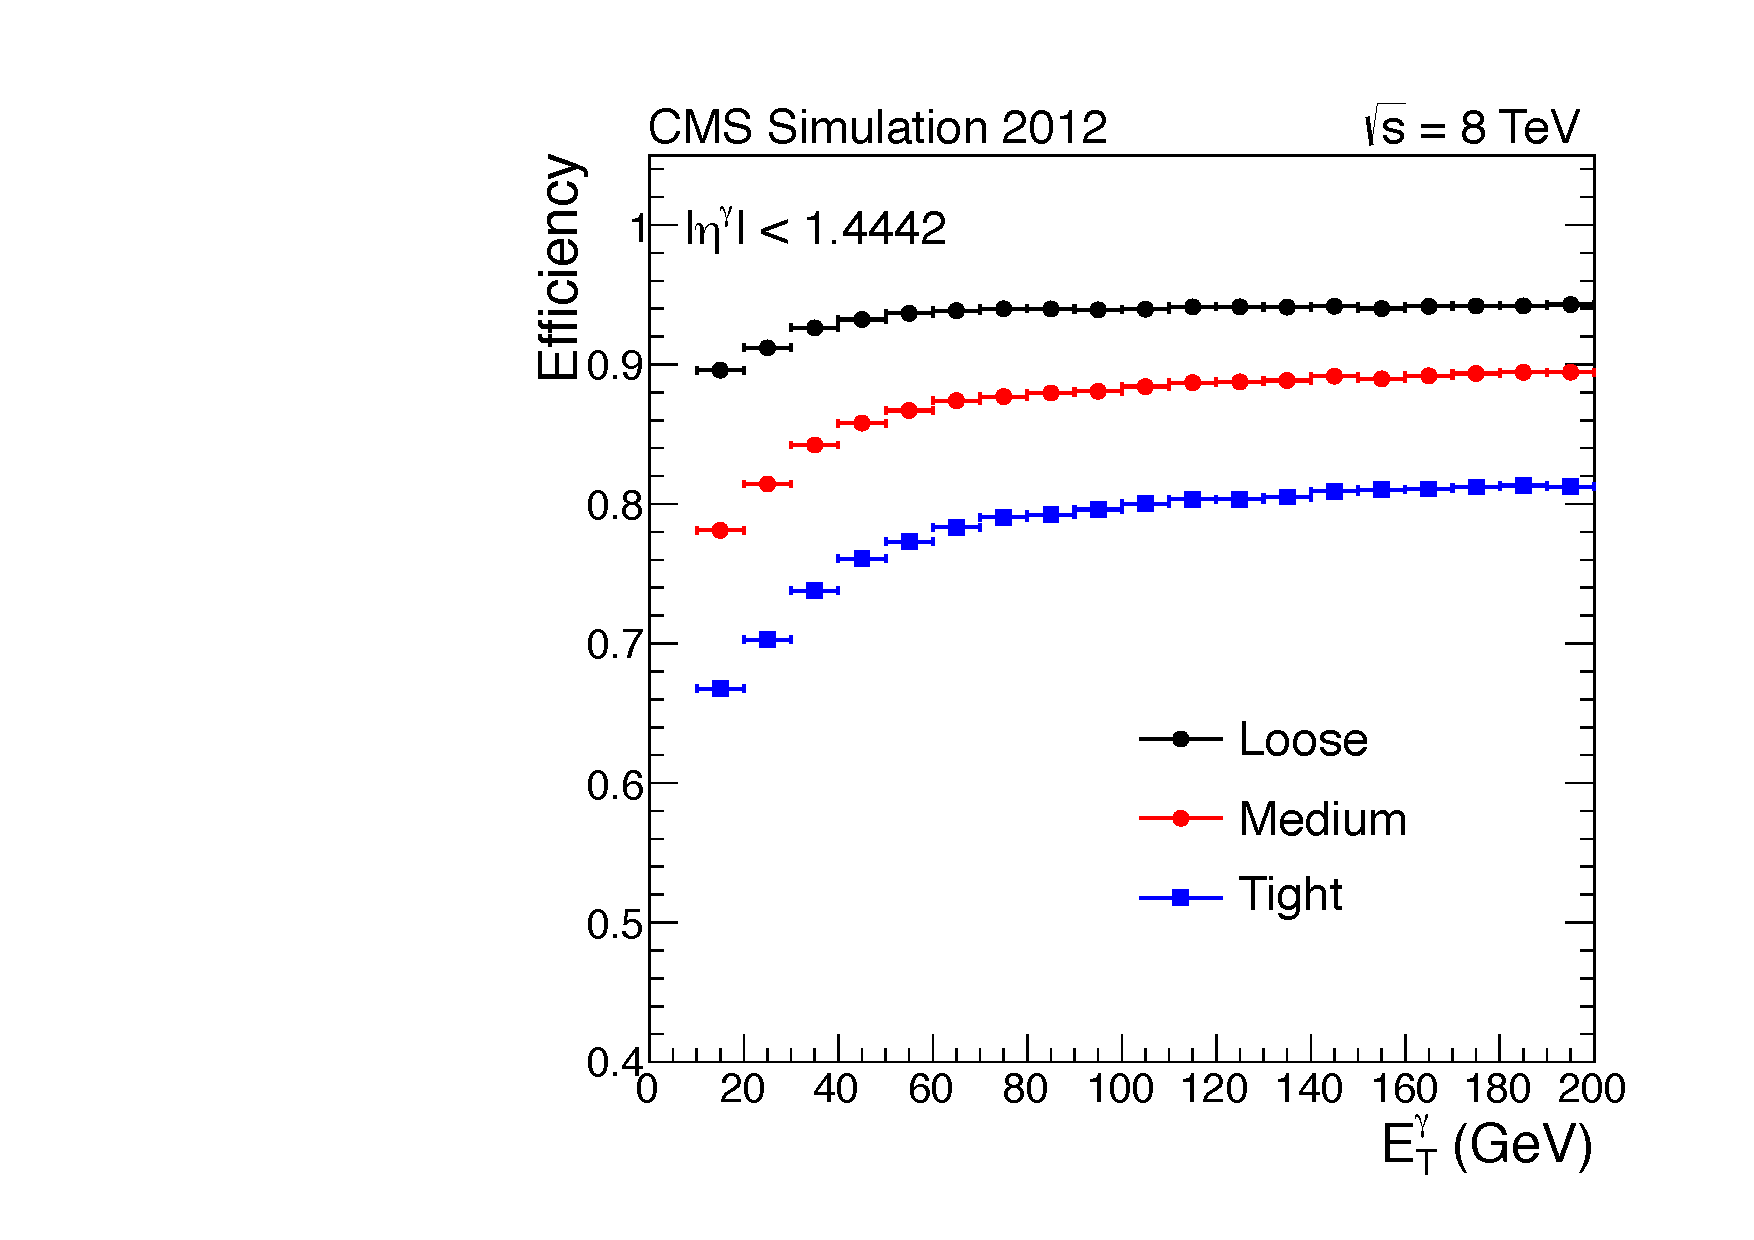
\includegraphics[width=0.44\textwidth]{chapitre3/figs/photon_eff.pdf}}
    \caption{(\subref{fig:mgg}) Distribution de la masse invariante $\gamma\gamma$ dans le tonneau obtenu à l'aide des données 2010, à l'aide d'une sélection optimisée pour les $\pi^0$. Le désaccord avec la mesure de la masse du $\pi^0 = \SI{135}{\MeV}$ est inférieur à \SI{1}{\%}. \citep{cms_pf_jets}. (\subref{fig:gamma_eff}) Efficacité d'identification des photons pour les trois points de fonctionnement recommandés par CMS \citep{cms_photon_perf}.}
    \label{fig:pf_photons}
\end{figure}

On présente \cref{fig:mgg} la résolution expérimentale obtenue lors de la reconstruction d'événement $\Ppizero \rightarrow \Pgamma \Pgamma$. On trouve une résolution $\sigma = \SI{13}{\MeV}$. L'efficacité d'identification pour les trois points de fonctionnement définis par la collaboration CMS est présentée \cref{fig:gamma_eff}. Dans tous les cas, cette efficacité est supérieure à \SI{65}{\%}.

\subsubsection{Isolation des leptons} \label{sec:lepton_isolation}

Bien souvent, il est important pour les analyses de physique de savoir si un lepton est isolé, c'est-à-dire de savoir si l'activité autour du lepton est faible. L'isolation du lepton est définie par la relation
\begin{align*}
  I_{\Plepton} &= \frac{\sum{\pt^\text{hadrons chargés}} + \sum{\pt^\text{hadrons neutres}} + \sum{\pt^\text{photons}}}{\pt^{\Plepton}}
\end{align*}
où les sommes portent sur les particules contenues dans un cône de rayon $\Delta R$ centré autour du lepton. Ainsi, plus $I$ tend vers 0, plus la particule est isolée. Deux valeurs de $\Delta R$ sont utilisées, suivant la saveur du lepton :
\begin{align*}
  \Delta R &= \num{0.4} \quad\text{muons}\\
  \Delta R &= \num{0.3} \quad\text{électrons}
\end{align*}

Dans le cas des muons, la définition de l'isolation $I$ est modifiée afin d'être plus robuste face au \pu. On considère en effet les hadrons chargés provenant d'un vertex autre que le vertex principal comme du \pu : ils ne sont donc pas utilisés dans le calcul de l'isolation. Ce n'est malheureusement pas suffisant, puisque le \pu est aussi composé de hadrons neutres et de photons : on estime que ces hadrons sont responsables d'environ la moitié de l'énergie du \pu. Ainsi, on soustrait du calcul de l'isolation la moitié de l'énergie des hadrons identifiés comme provenant du \pu, en vérifiant bien que l'énergie provenant de la partie neutre ne soit jamais négative. On obtient alors
\begin{align*}
  I_{\Pmu}^\text{corrigé} &= \frac{\sum{\pt^\text{hadrons chargés}} + \overbrace{\left(\sum{\pt^\text{hadrons neutres}} + \sum{\pt^\text{photons}} - \num{0.5} \sum{\pt^\text{hadrons chargés \pu}} \right)}^{= 0 \text{ si négatif}}}{\pt^{\Plepton}}
\end{align*}
On considère un muon comme isolé si $I_{\Pmu}^\text{corrigé} < \SI{12}{\%}$.

\smallskip

Pour les électrons, on applique une procédure similaire. Néanmoins, au lieu de soustraire la moitié de l'énergie des hadrons chargés provenant du \pu, on estime l'énergie restant due au \pu en utilisant la densité d'énergie dans l'événement par unité de surface ($\rho$, voir \cref{sec:jec_l1}). Au lieu d'utiliser la surface du cône d'isolation, parfois délicate à calculer géométriquement, pour estimer la quantité d'énergie du \pu, on évalue une surface effective ($EA$) sur des événements \PZ $\rightarrow$ \Pelectron{}\Ppositron.% Cette surface est définie comme le rapport entre la pente de la droite $\rho = f(N_{\text{vertex}})$ et la pente de la droite $I = f(N_\text{vertex})$. \fxnote{Revoir la partie sur EA.}
\begin{align*}
  I_{\Pe}^\text{corrigé} &= \frac{\sum{\pt^\text{hadrons chargés}} + \overbrace{\left(\sum{\pt^\text{hadrons neutres}} + \sum{\pt^\text{photons}} - \rho\,EA \right)}^{= 0 \text{ si négatif}}}{\pt^{\Plepton}}
\end{align*}
On considère un électron comme isolé si $I_{\Pe}^\text{corrigé} < \SI{10}{\%}$. Cette valeur est plus faible en raison de la taille du cône plus faible également.

\subsection{Calibration des calorimètres}

\begin{figure}[tbp]
    \centering
    \subcaptionbox{\label{fig:hadron_calib_barrel}}[0.48\textwidth]{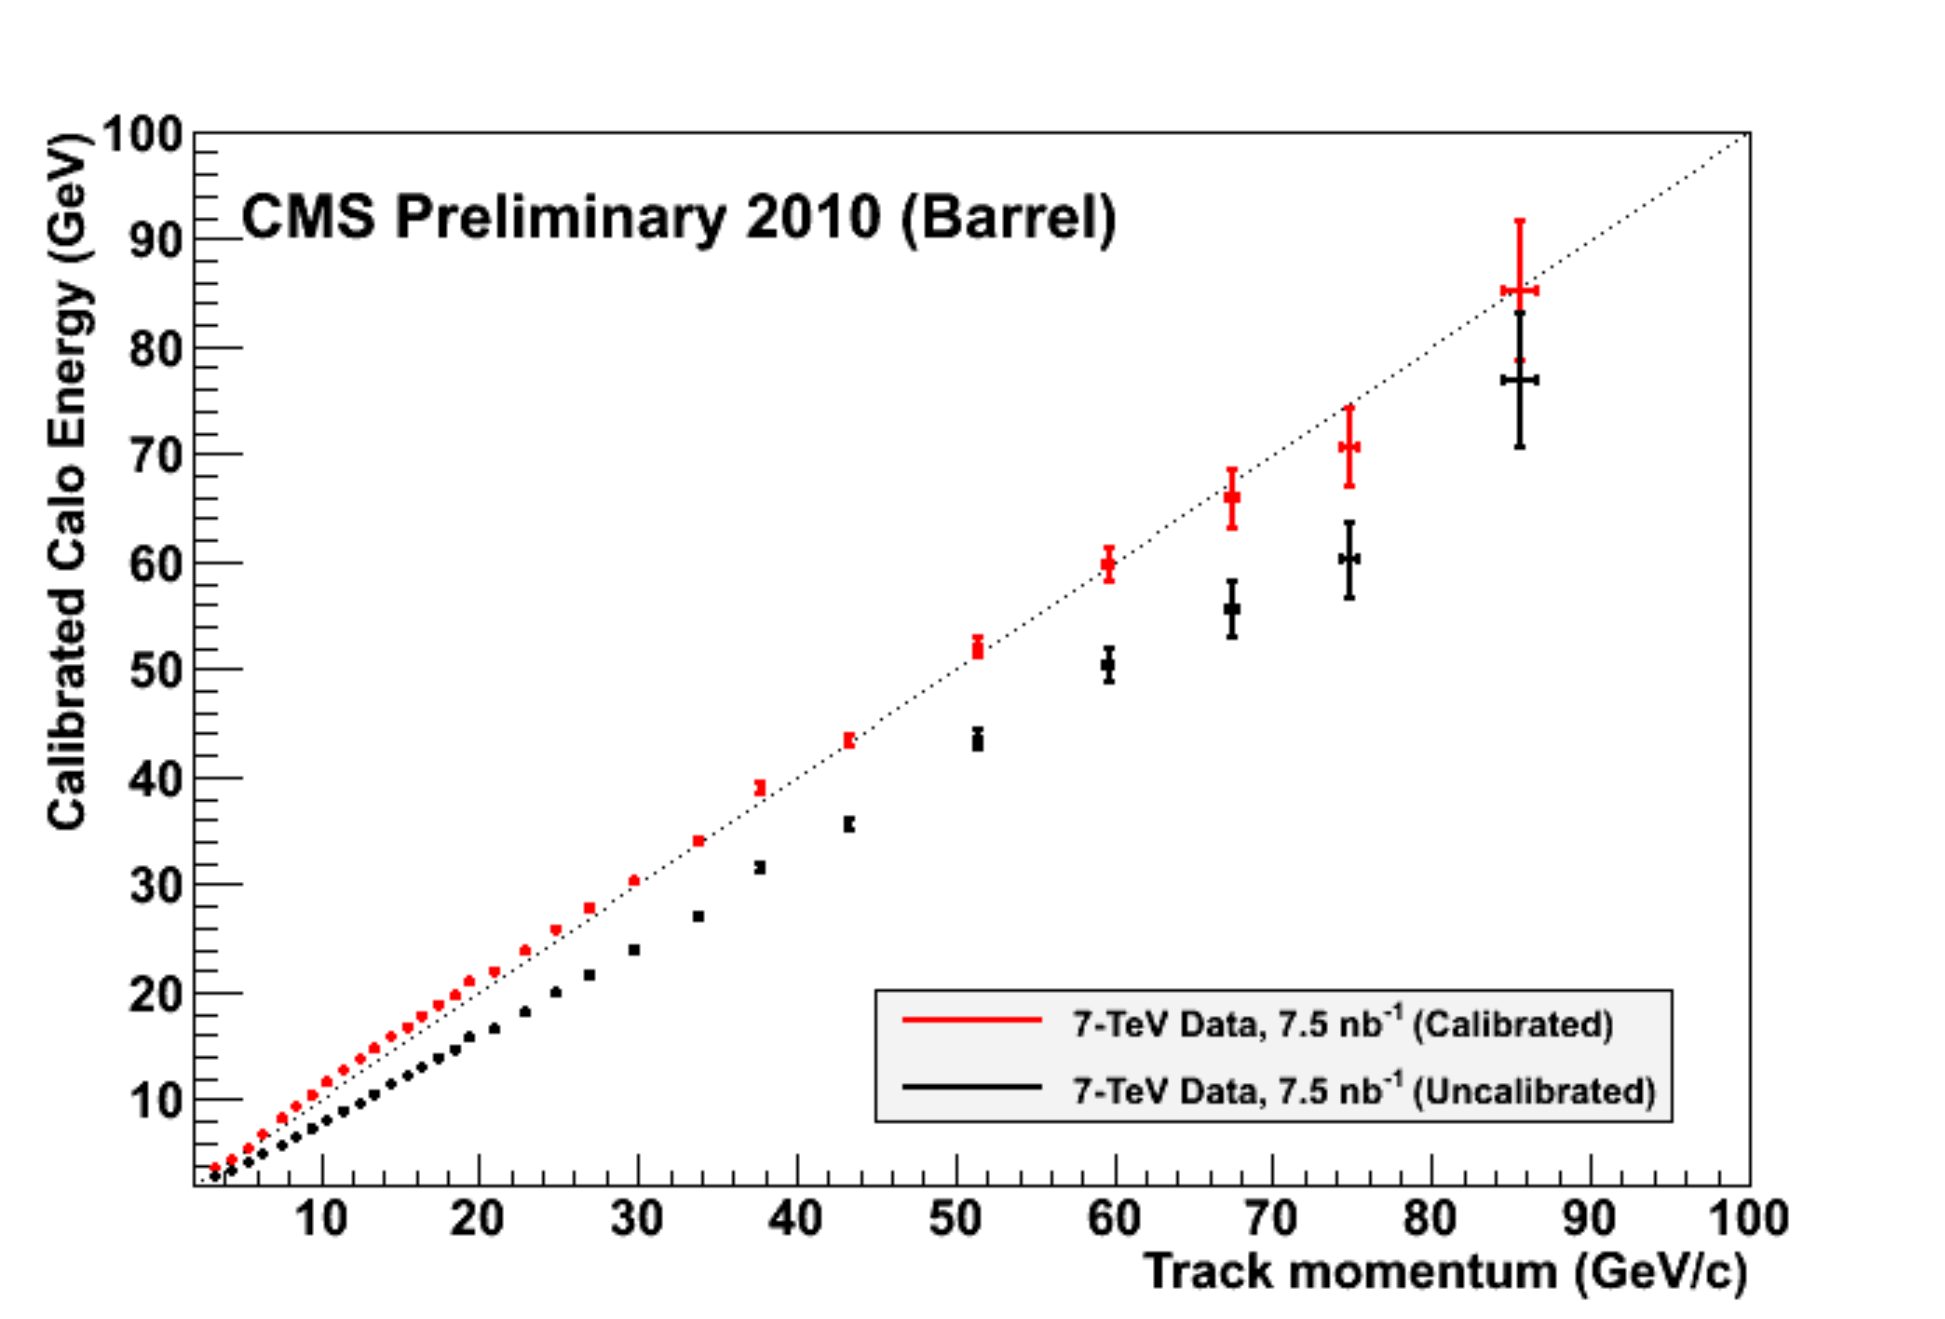
\includegraphics[width=0.48\textwidth]{chapitre3/figs/hadron_calib_barrel.png}} \hfill
    \subcaptionbox{\label{fig:hadron_calib_endcap}}[0.48\textwidth]{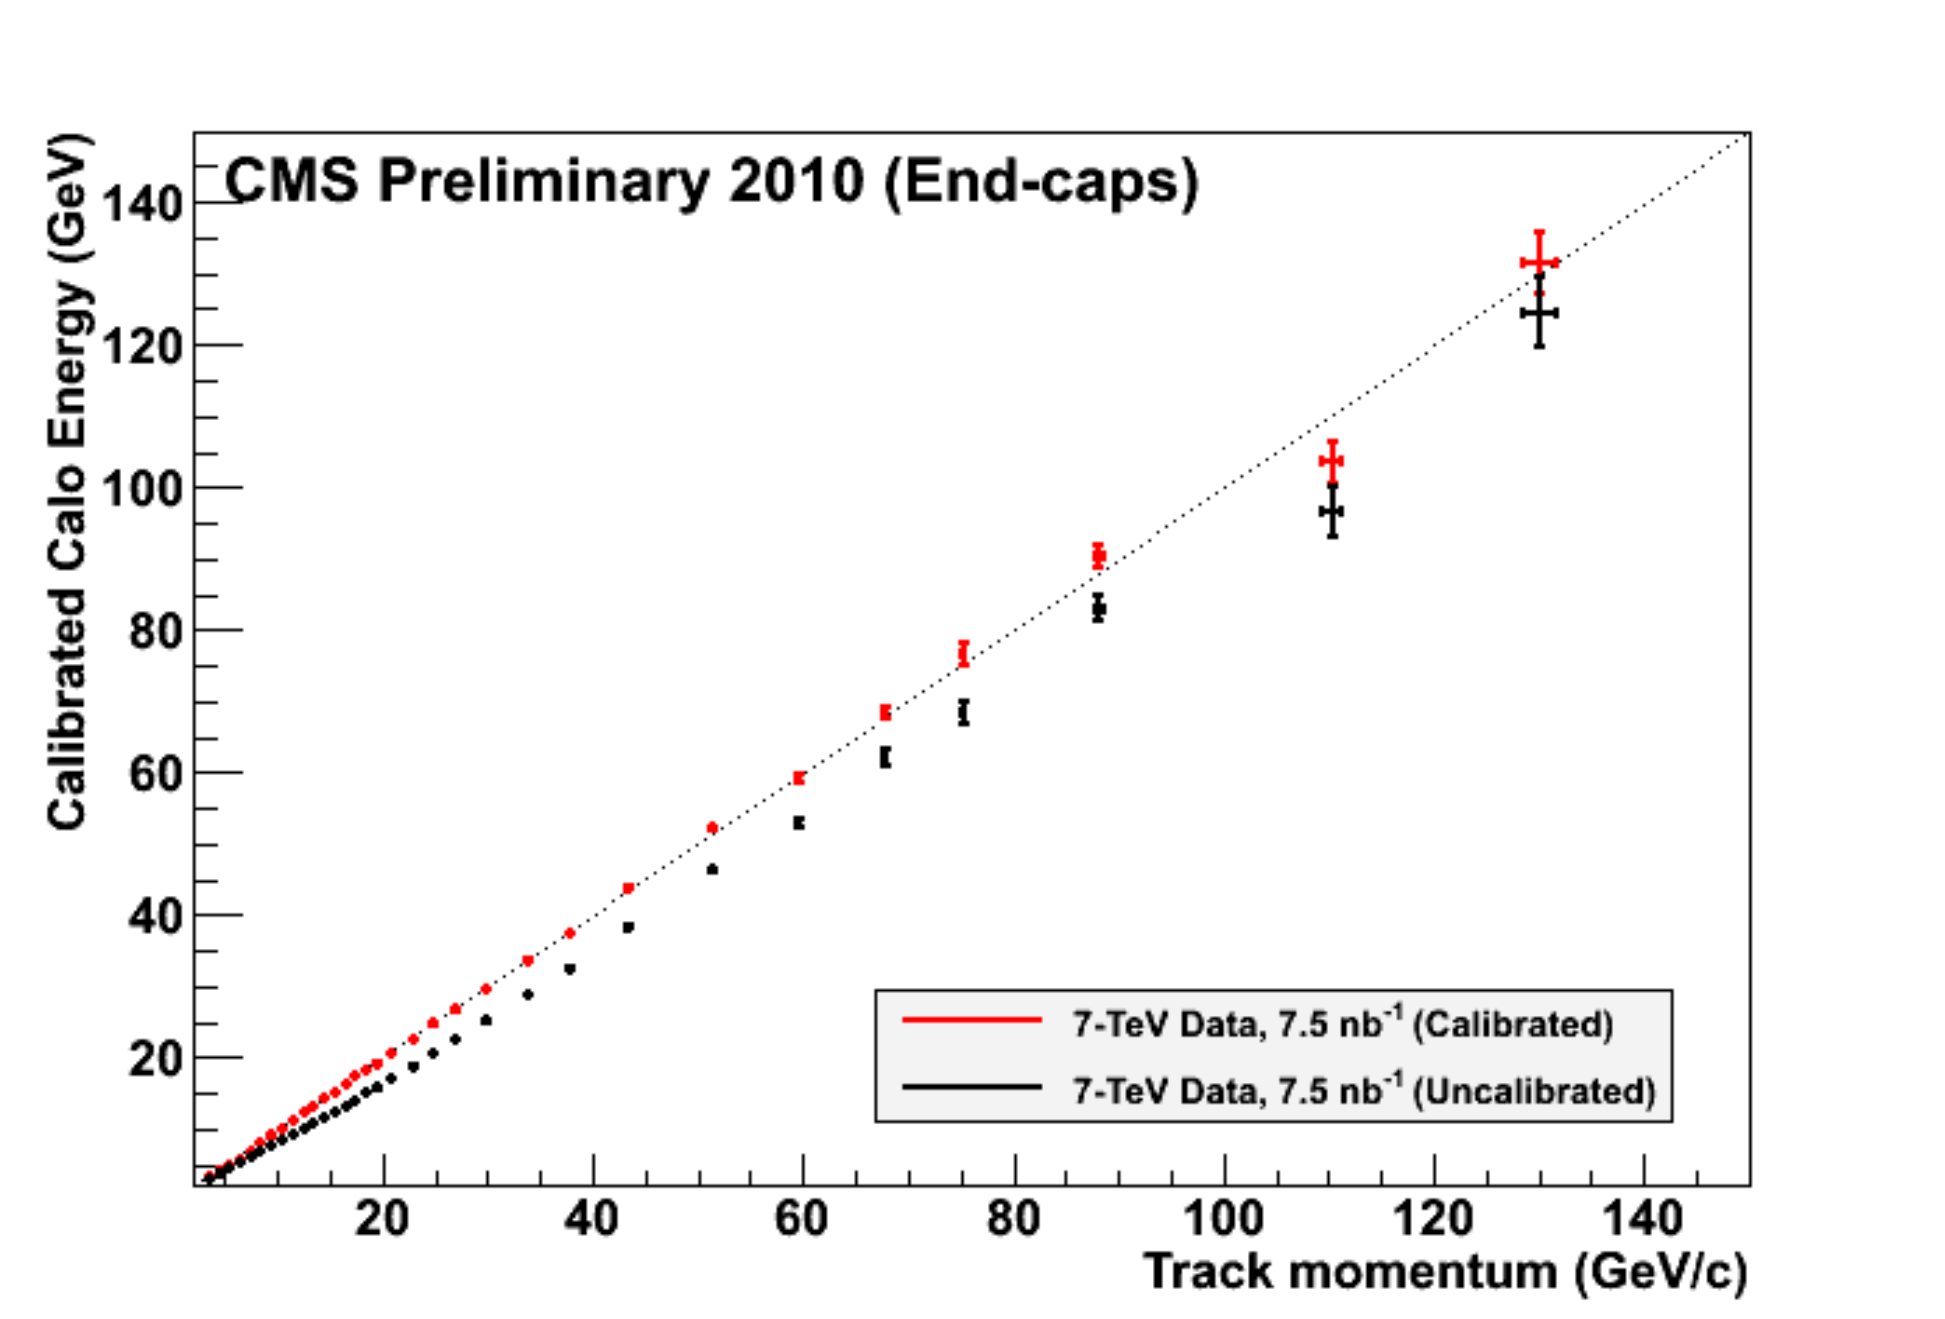
\includegraphics[width=0.48\textwidth]{chapitre3/figs/hadron_calib_endcap.png}}
    \caption{Effet de la calibration de l'énergie des hadrons chargés dans le tonneau (\subref{fig:hadron_calib_barrel}) et dans les bouchons (\subref{fig:hadron_calib_endcap}).}
    \label{fig:hadron_calib}
\end{figure}

Afin d'estimer au mieux l'énergie des particules reconstruites, les calorimètres doivent être calibrés en fonction du type de particules reconstruites. Par exemple, la réponse du calorimètre pour les photons ou les hadrons chargés n'est pas identique.

Pour les électrons et les photons, des corrections sont dérivées en utilisant la simulation comme référence, et en exploitant des processus physiques bien connu, tel que $\PZ \rightarrow \Pelectron \Ppositron$ pour la calibration des électrons ou $\PZ \rightarrow \Pmuon \APmuon \Pphoton$ pour la calibration des photons.

Pour les hadrons chargés, l'énergie calorimétrique associée au bloc \emph{particle-flow} est calibrée par la fonction
\begin{align*}
  E_\text{calib} &= a + b\left(E, \eta\right) E_\text{ECAL} + c\left(E, \eta\right)E_\text{HCAL}
\end{align*}
où $a$, $b$, $c$ sont des constantes de calibration à déterminer, $E$ l'énergie totale non calibrée du hadron chargé, et $\eta$ la pseudo-rapidité de la cellule du HCAL. Ces constantes ont été déterminées sur les premières données en 2010. On peut voir \cref{fig:hadron_calib} l'effet de la calibration sur la détermination de l'énergie des hadrons chargés. Cette calibration impacte directement la mesure de l'énergie des photons et des hadrons neutres. Elle est donc primordiale.

\subsection{Reconstruction des jets} \label{sec:jet_reco}

% \begin{figure}[tbp]
%     \centering
%     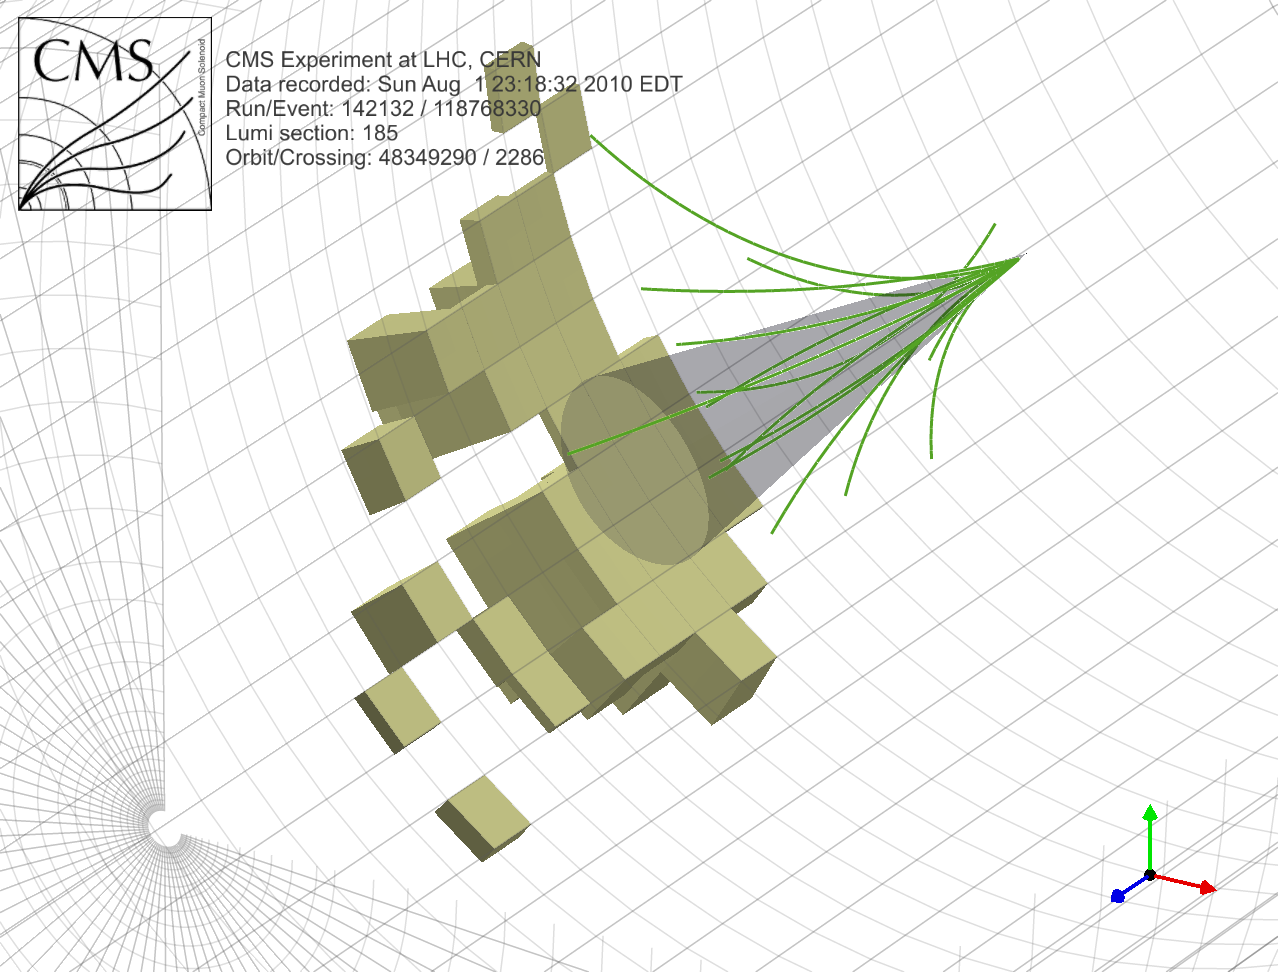
\includegraphics[width=0.5\textwidth]{chapitre3/figs/jet.png}
%     \caption{Reconstruction d'un jet dans CMS. Les traces et les dépôts calorimétriques ont été rendus visible.}
%     \label{fig:jet}
% \end{figure}

A cause du confinement lié à l'interaction forte, les quarks et gluons produits lors des collisions ne peuvent pas être observés directement. En effet, lors de leurs propagations, ils vont se combiner avec d'autre quarks pour former des hadrons. On obtient alors une cascade d'hadronisation, et on détecte ainsi une gerbe de particules en lieu et place d'un quark. Cette gerbe de particules, formées principalement de hadrons, mais aussi de leptons, est appelée \emph{jet}. %On peut voir \cref{fig:jet} la reconstruction d'un jet dans CMS. On voit bien une grande quantité de traces, associées à l'hadronisation d'un quark ou d'un gluon.

Grâce à l'algorithme de \emph{particle-flow}, on dispose d'une description globale de l'événement, sous forme d'une liste de particules. On utilise des algorithmes spécialisés qui vont parcourir la liste des particules, et former des agrégats suivant certains critères de distance entre les particules, différents selon les algorithmes. CMS utilise majoritairement deux types d'algorithmes : l'algorithme \emph{anti-$k_T$} \citep{antikt} et l'algorithme \emph{Cambridge-Aachen} (C-A) \citep{ca_jets}. Ce dernier est principalement utilisé lorsque l'on cherche une possible sous-structure au sein d'un jet. Par exemple, dans le cas de la désintégration d'un boson $W$ de très grande impulsion, les deux quarks peuvent être produits de façon très colinéaire, entraînant la reconstruction d'un seul gros jet, au lieu de deux.

Dans le but d'éviter d’agréger au sein d'un jet des leptons isolés, on commence par les supprimer de la liste des particules. On évite ainsi des double comptage de l'énergie, où un lepton pourrait se trouver dans une collection leptons mais aussi dans un jet. On définit l'isolation d'un lepton comme le rapport entre l'énergie des particules contenues dans un cône de rayon $\Delta R$, centré sur le lepton, sur l'énergie de ce lepton. En dessous d'un certain seuil (typiquement, \num{10} ou \SI{12}{\%}), on considère le lepton isolé.

\medskip

\begin{figure}[tbp]
    \centering
    \subcaptionbox{\label{fig:jets_akt}}[0.45\textwidth]{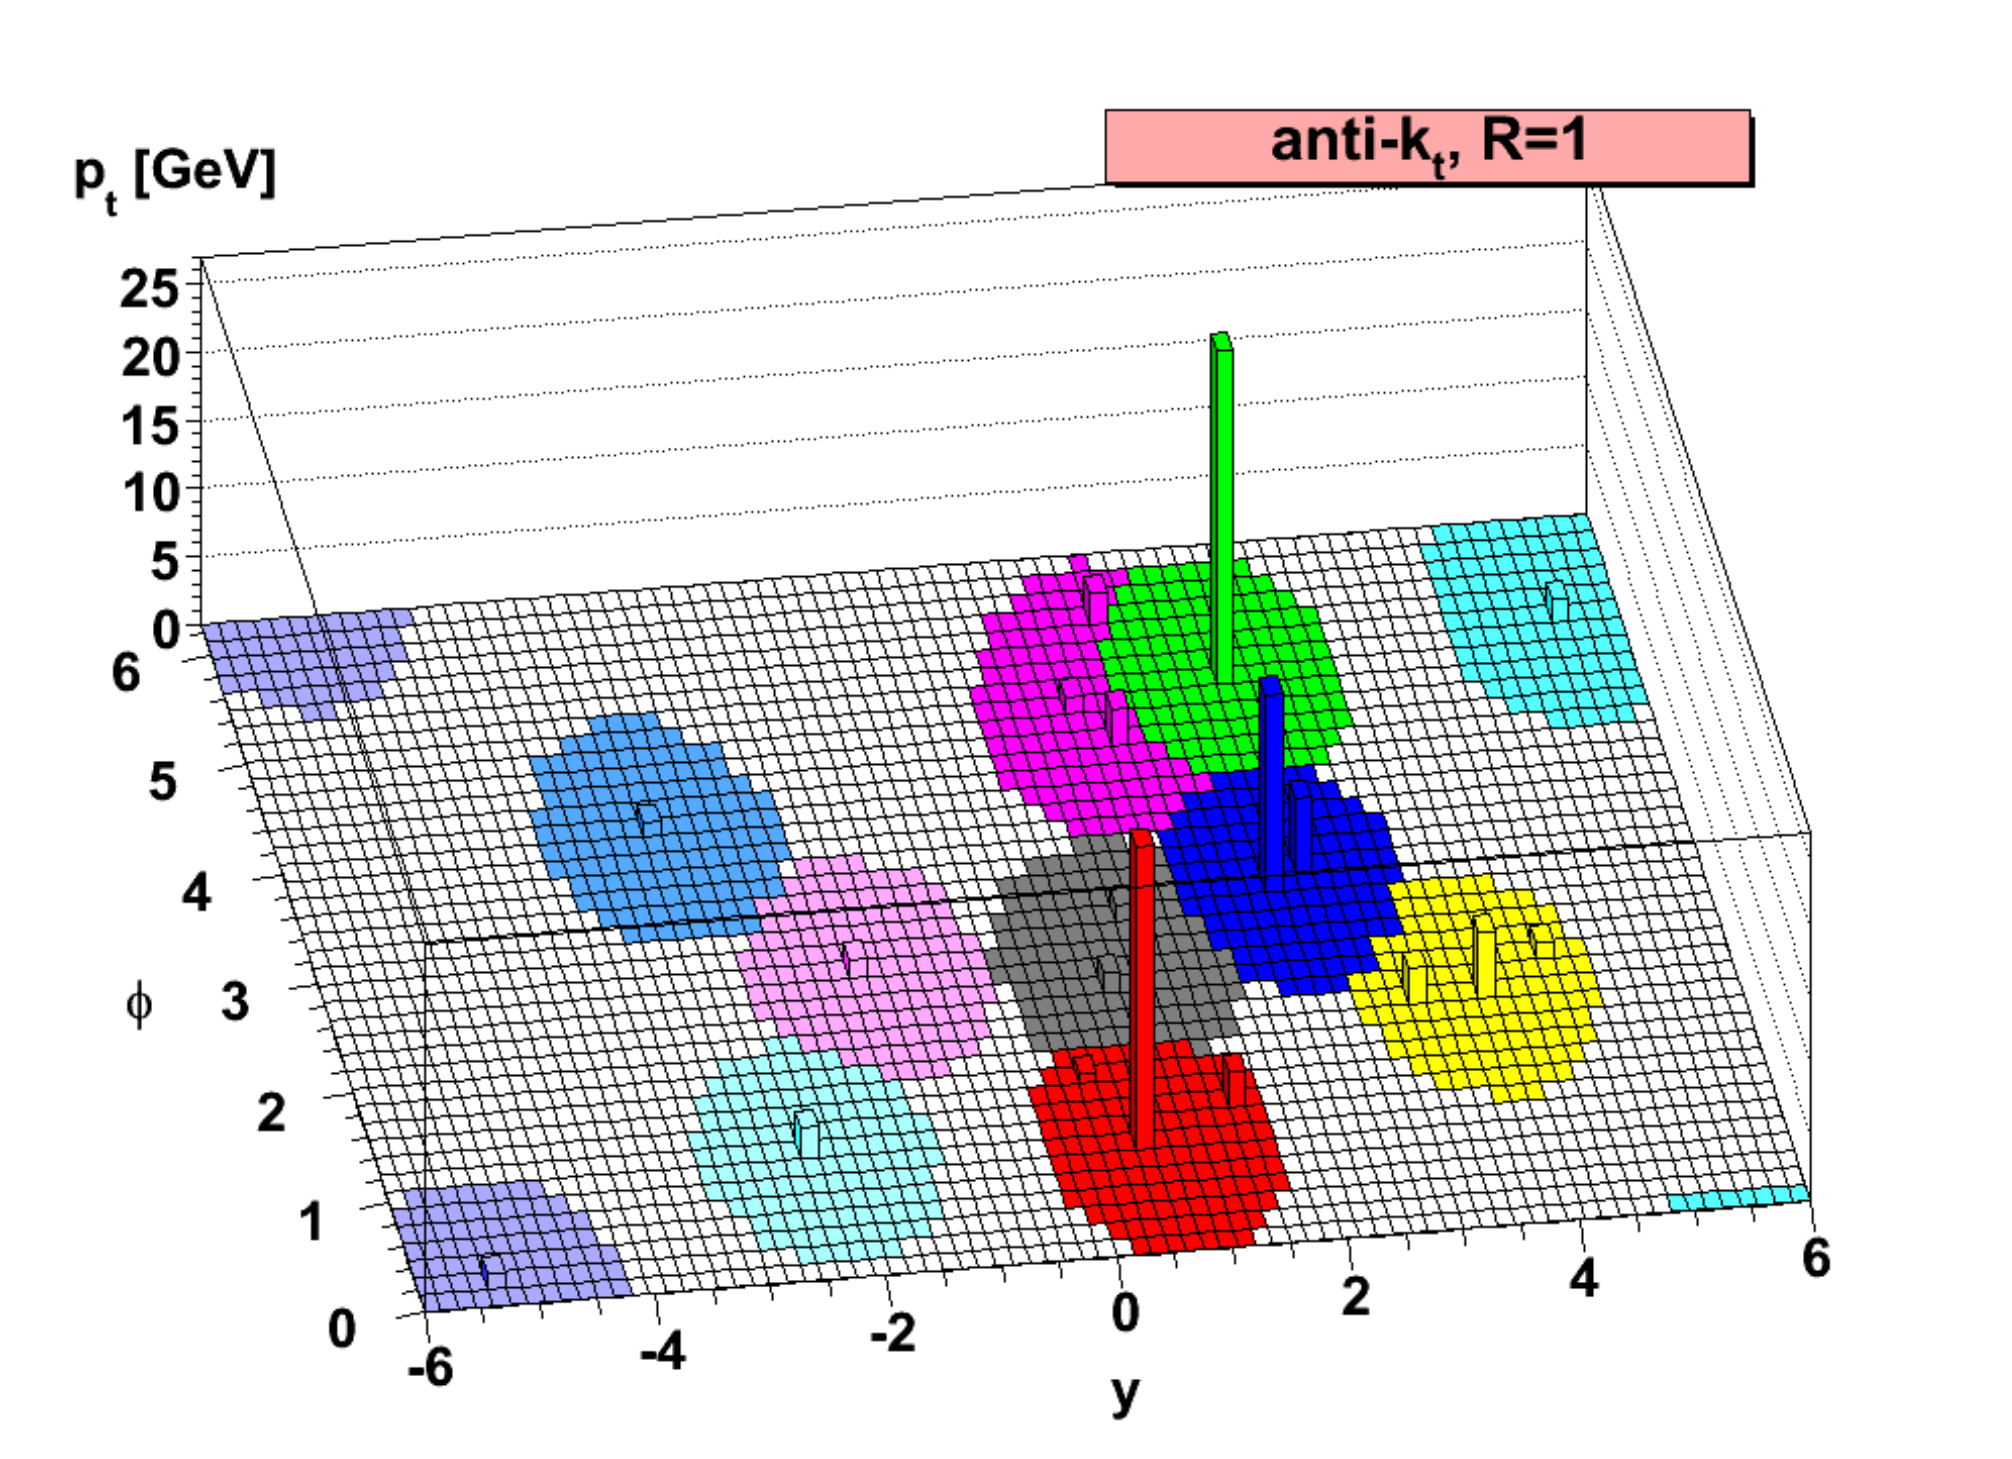
\includegraphics[width=0.45\textwidth]{chapitre3/figs/jets_akt.png}} \hfill
    \subcaptionbox{\label{fig:jets_ca}}[0.45\textwidth]{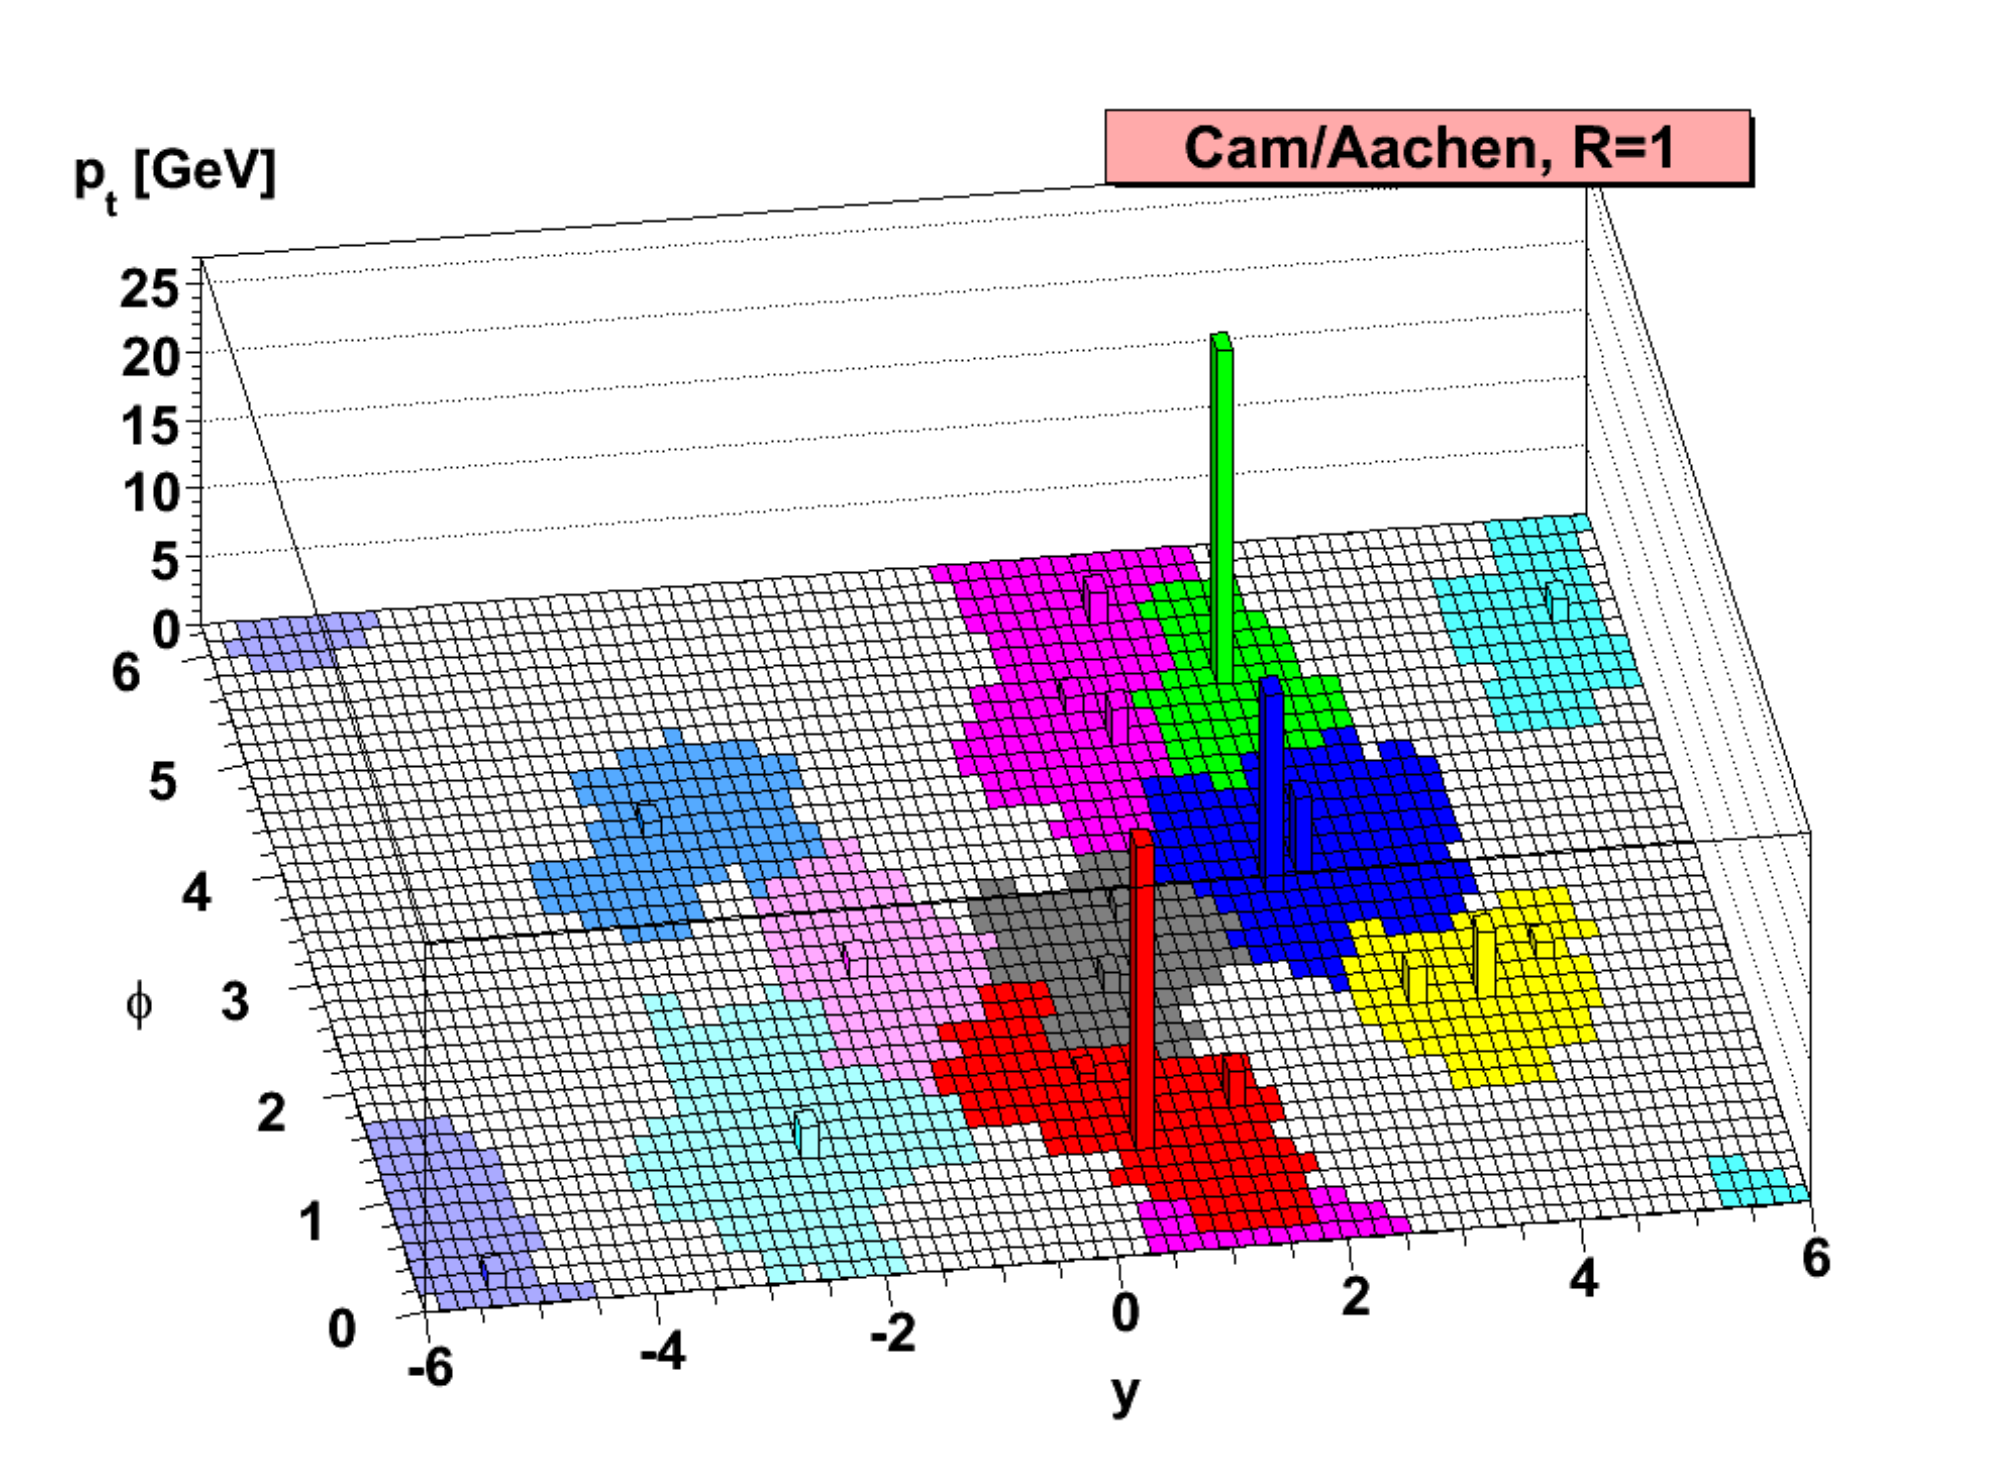
\includegraphics[width=0.45\textwidth]{chapitre3/figs/jets_ca.png}}
    \caption{Reconstruction des jets dans le plan ($\eta$, $\phi$) effectuée sur le même événement par l'algorithme anti-$k_T$ (\subref{fig:jets_akt}) et par l'algorithme C-A (\subref{fig:jets_ca}), pour une distance $R = 1$ \citep{antikt}.}
    \label{fig:akt_ca}
\end{figure}

Les deux algorithmes précédemment mentionné itèrent sur la collection de particules, et tentent de construire un jet en associant les particules deux à deux. Pour ce faire, ils utilisent les quantités suivantes :
\begin{align*}
  d{ij} &= \text{min}\left( k_{T, i}^n, k_{T, j}^n \right) \frac{\Delta R^2_{ij}}{R^2} \\
  d_{iB} &= k^n_{T, i}
\end{align*}
où $k_{T, i}$ est l'impulsion transverse de la particule $i$ par rapport à l'axe du faisceau, $\Delta R_{ij}$ la distance entre $i$ et $j$ dans le plan ($\eta$, $\phi$), et $R$ une distance, choisie par l'utilisateur, symbolisant la largeur du jet. Pour l'algorithme \emph{anti-$k_T$}, on a $n = -2$, tandis que pour C-A, on a $n = 1$. $d_{iB}$ est un estimateur de la distance entre la particule $i$ et le faisceau.

L'algorithme cherche la valeur minimum $d_{min}$ entre tous les $d_{ij}$ et $d_{iB}$. Si le minimum est obtenu pour une valeur de $d_{ij}$, les particules $i$ et $j$ sont fusionnées (leurs quadrivecteurs sont sommés), et l'algorithme recommence. Au contraire, si le minimum est obtenu pour $d_iB$, la particule $i$ (souvent résultant de la fusion de plusieurs autres particules lors des itérations précédentes de l'algorithme) est considérée comme un jet et enlevée de la liste des particules. L'algorithme stoppe quand aucune particule ne reste.

La seule différence entre ces deux algorithmes vient de la façon dont le choix des particules à grouper est fait. Pour l'algorithme \emph{anti-$k_T$}, le poids de chaque paire est proportionnel à $\text{min}\left( 1 / k^2_{T,i}, 1 / k^2_{T,j} \right)$, ce qui revient à fusionner les particules de grande impulsions les plus proches en premier. Dans le cas de l'algorithme C-A, le poids est uniquement proportionnel à la distance entre les paires : les particules les plus proches sont fusionnées en premier. On peut voir \cref{fig:akt_ca} un exemple de reconstruction des jets sur un même événement par les deux algorithmes.

\bigskip

Une alternative à la reconstruction des jets \emph{particle-flow} existe, utilisant les amas calorimétriques en entrée des algorithmes de reconstructions des jets. Cette méthode était utilisée par CMS avant la mise en place du \pf, bien plus performant. On présente \cref{fig:pf_vs_calo_jets_reso} la résolution des jets pour l'algorithme \emph{particle-flow} (pf-jets) et la reconstruction calorimétrique (calo-jets). On voit très nettement l'amélioration apportée par la reconstruction \emph{particle-flow}. On présente également \cref{fig:pf_jets_composition} la composition des jets \pf reconstruit sur les données. Les jets sont constitués majoritairement de hadrons chargés et de photons.

\begin{figure}[tbp]
    \centering
    \subcaptionbox{\label{fig:pf_vs_calo_jets_reso}}[0.45\textwidth]{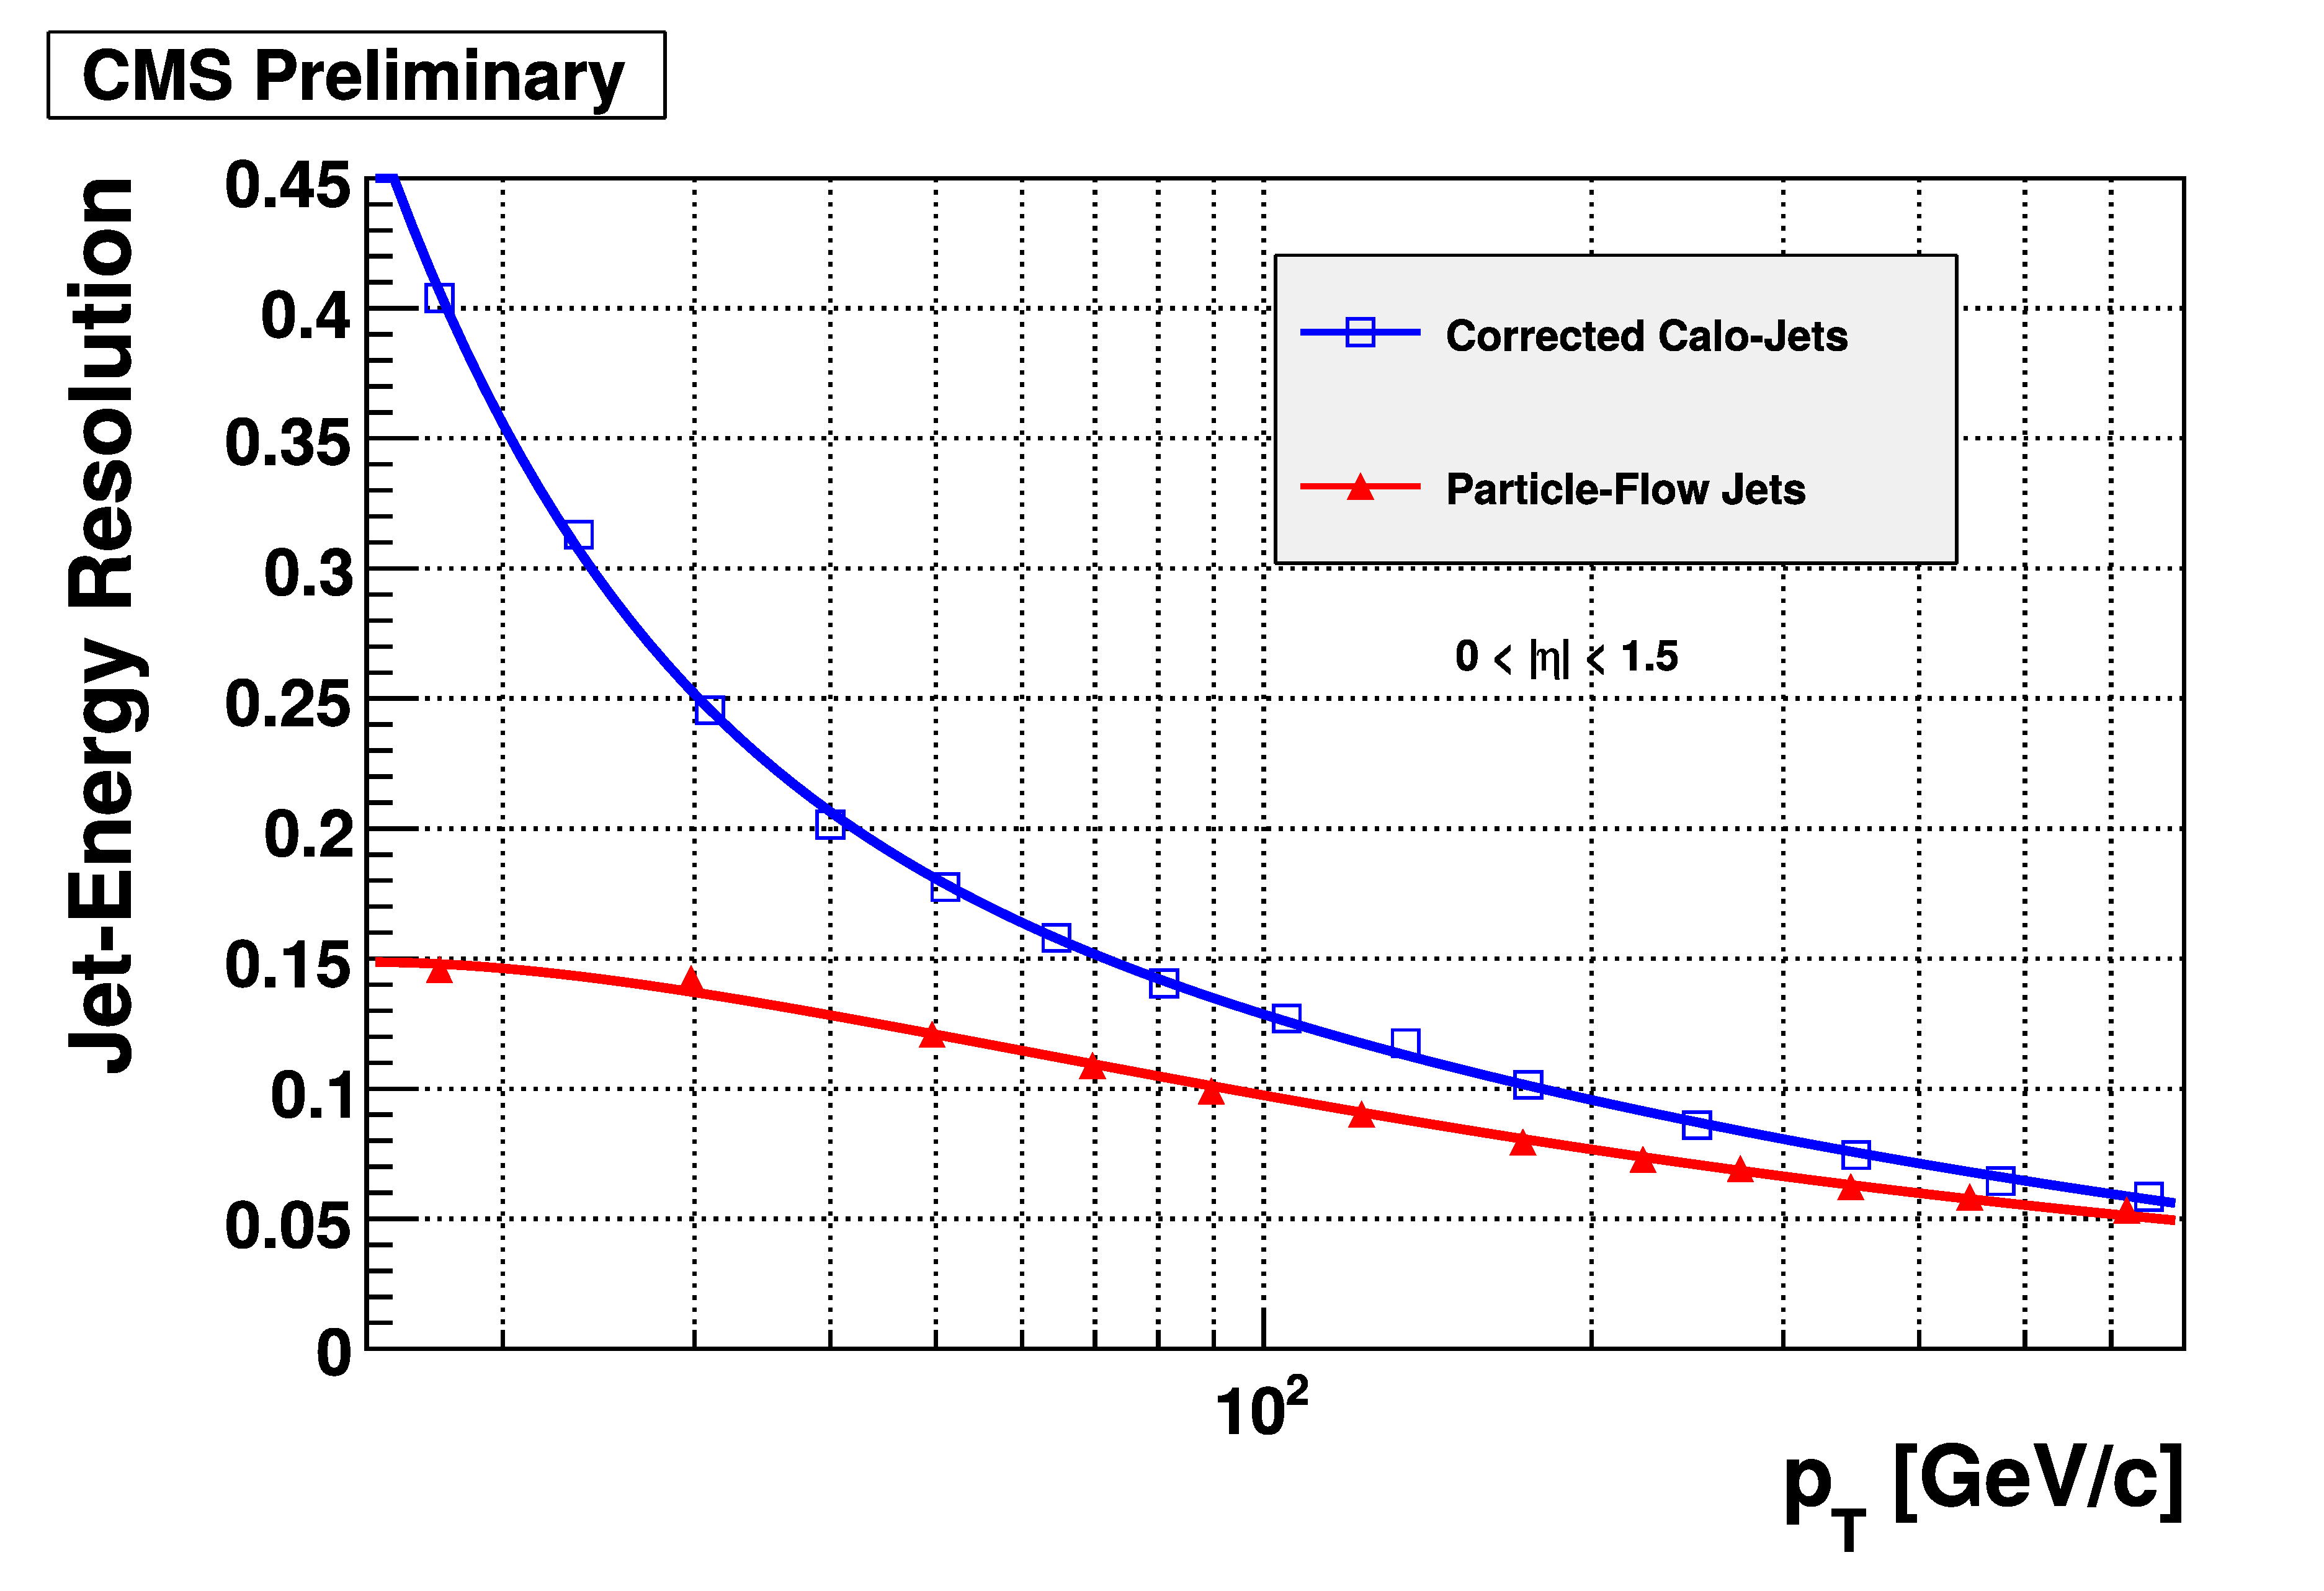
\includegraphics[width=0.45\textwidth]{chapitre3/figs/pf_vs_calo_jets.pdf}} \hfill
    \subcaptionbox{\label{fig:pf_jets_composition}}[0.45\textwidth]{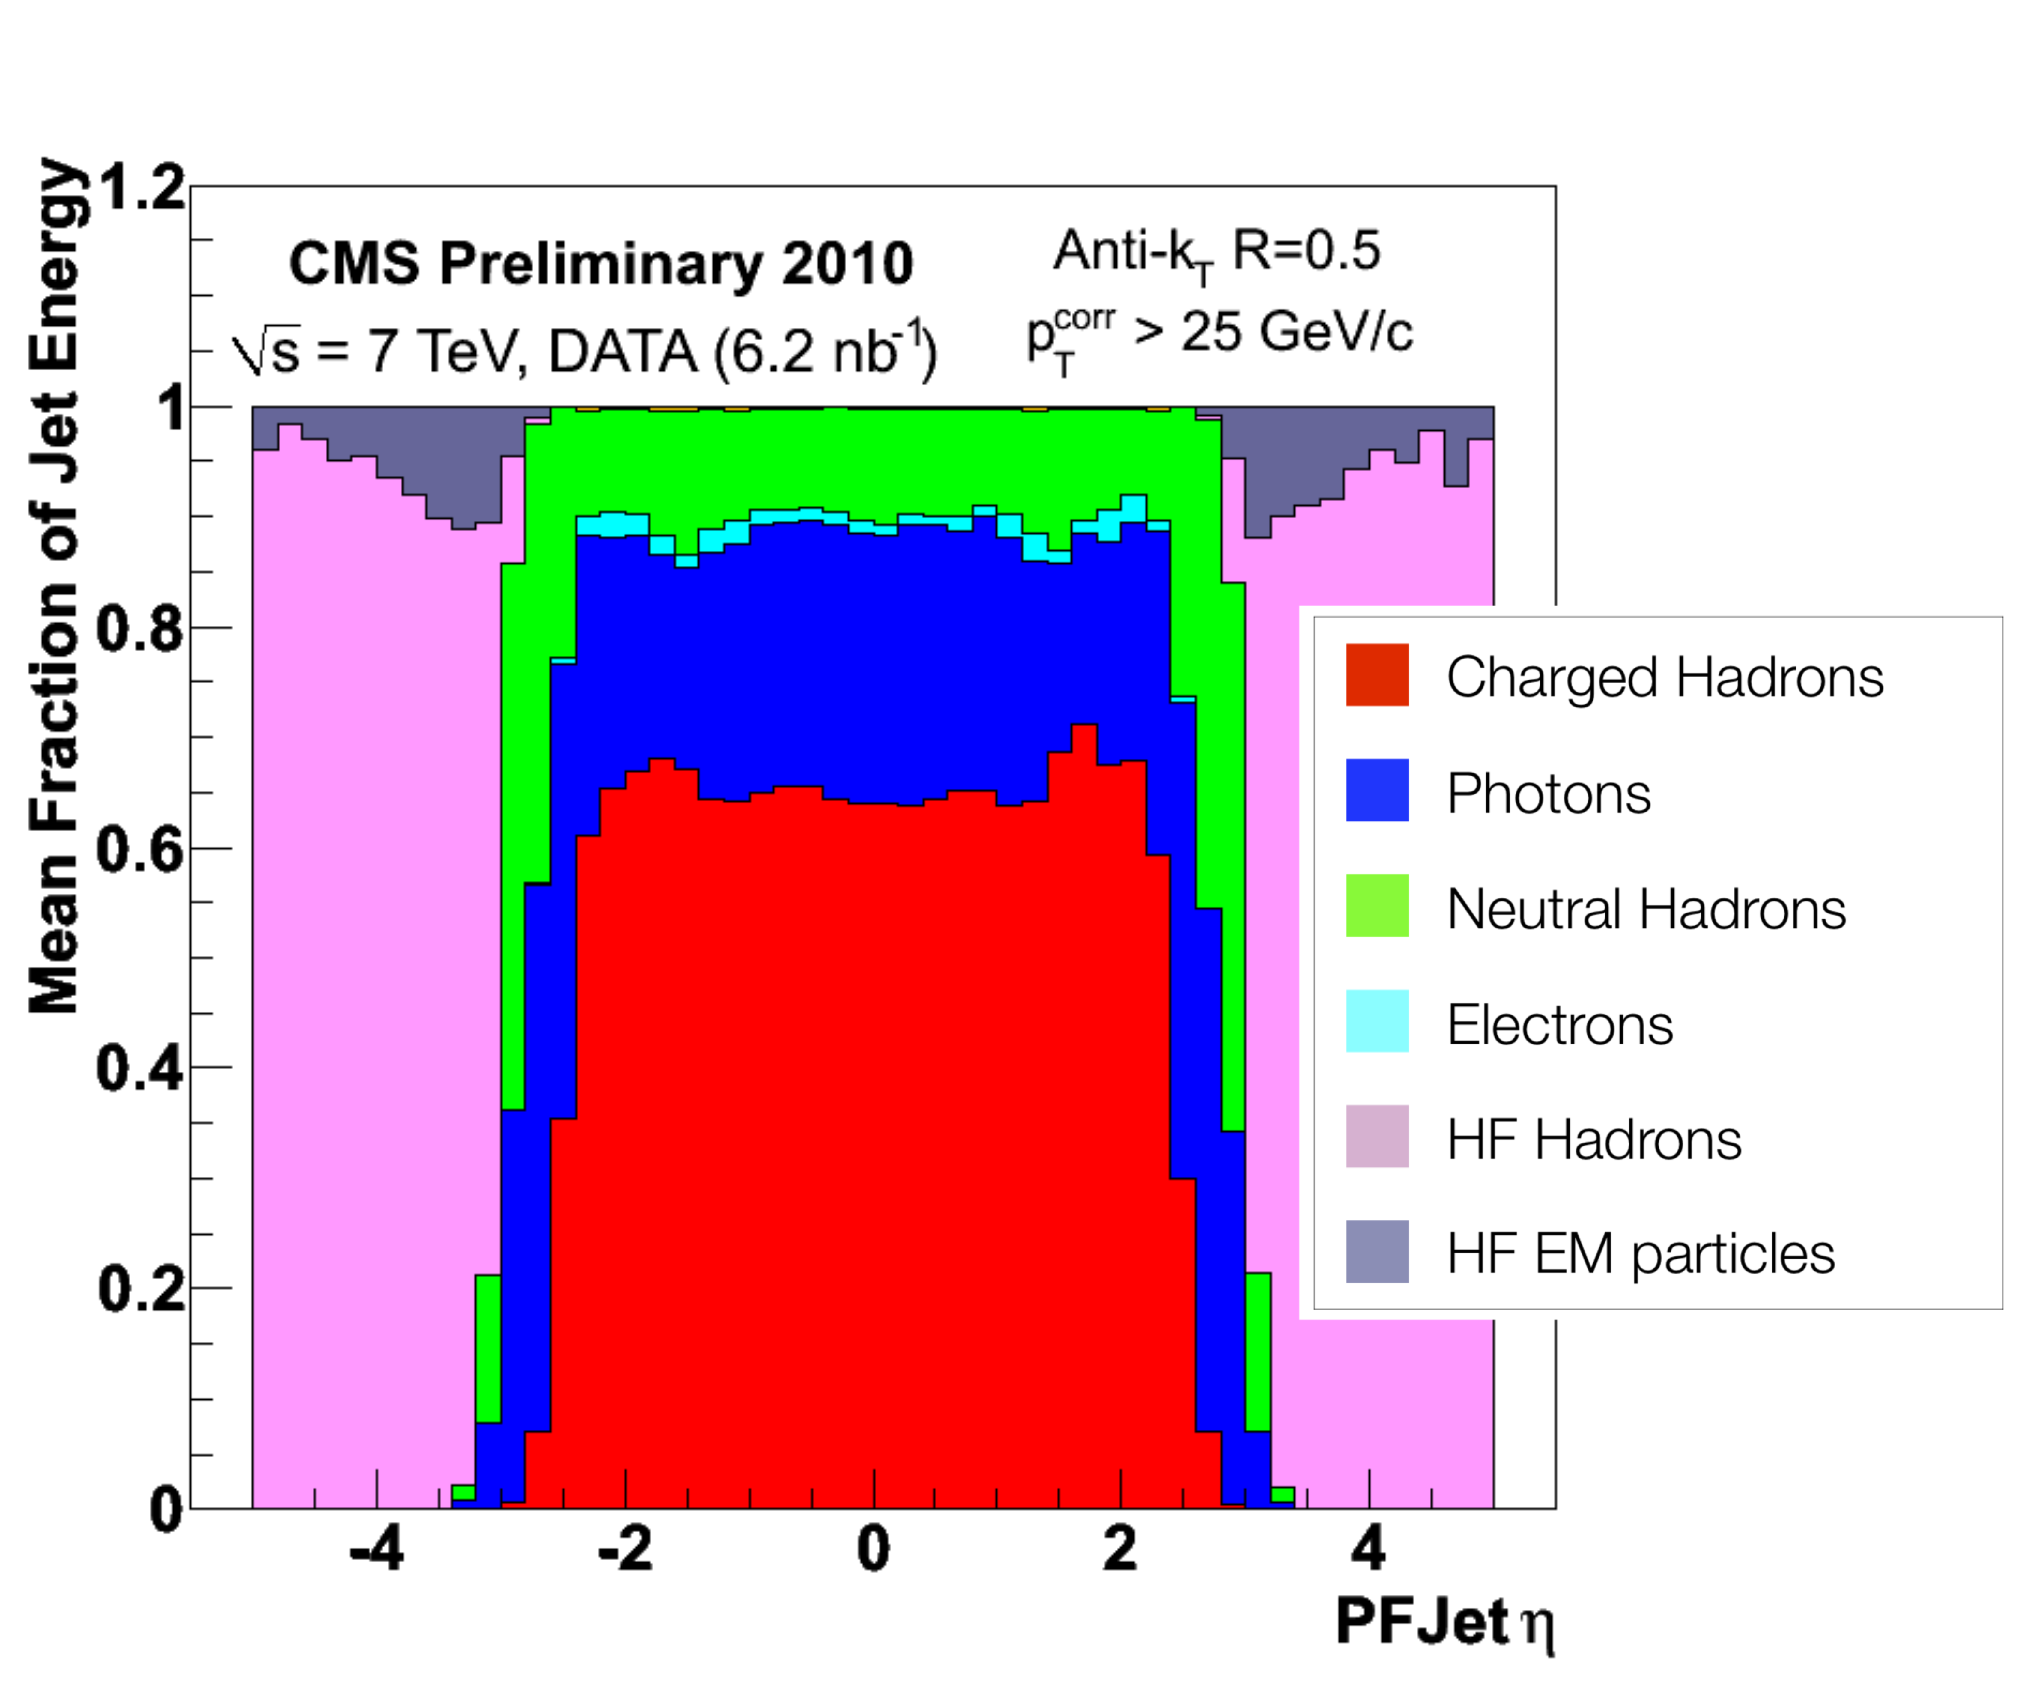
\includegraphics[width=0.45\textwidth]{chapitre3/figs/pf_jets_composition.png}}
    \caption{(\subref{fig:pf_vs_calo_jets_reso}) Résolution sur la reconstruction des jets \emph{particle-flow} (rouge) et calorimétriques (bleu) et (\subref{fig:pf_jets_composition}) composition énergétique des jets \emph{particle-flow}. La proportion de hadrons chargés chute brutalement à partir de $\abs{\eta} > 2.4$, puisque le trajectographe n'est plus disponible pour les identifier \citep{cms_pf_jets}.}
    \label{fig:pf_jets_perf}
\end{figure}

\subsubsection{Correction de l'énergie des jets}

L'énergie des jets reconstruits nécessite d'être calibrée pour plusieurs raisons. Premièrement, il arrive que des particules créées lors de l'hadronisation ne soient pas correctement agglomérées dans le jet, souvent parce que la trajectoire de ces particules dévie trop de la trajectoire initiale du quark. Enfin, des problèmes de calibrations des sous-détecteurs viennent aussi dégrader la mesure de l'énergie des jets.

La calibration des jets est effectuée en différentes étapes, présentées en détails dans le \cref{chap:jetmet}.

\subsubsection{L'algorithme d'identification des jets de $b$} \label{sec:b_tagging}

\begin{figure}[tbp]
    \centering
    \subcaptionbox{\label{fig:btag_discri}}[0.45\textwidth]{\includegraphics[width=0.45\textwidth]{chapitre3/figs/btag_tt_csv.pdf}} \hfill
    \subcaptionbox{\label{fig:btag_csv_eff}}[0.45\textwidth]{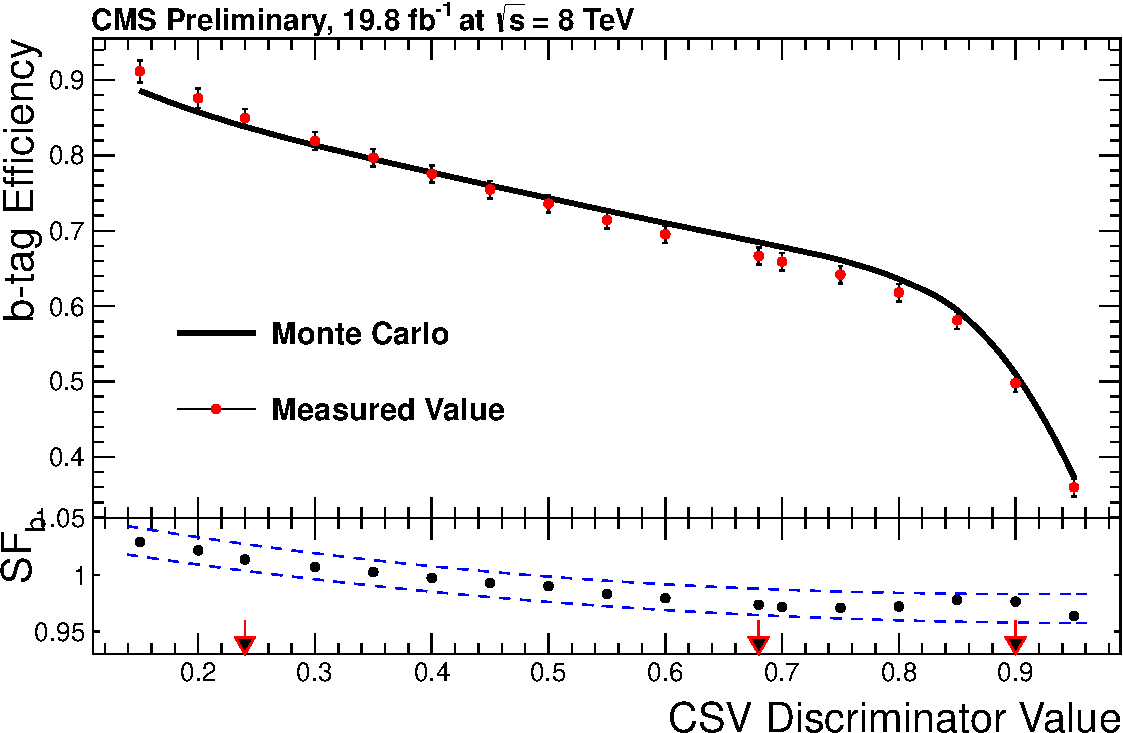
\includegraphics[width=0.45\textwidth]{chapitre3/figs/btag_csv_eff.pdf}}
    \caption{(\subref{fig:btag_discri}) Sortie de l'analyse multivariée de l'algorithme CSV sur un échantillon enrichi \ttbar. Les hautes valeurs sont enrichies en quark $b$, et les trois flèches correspondent aux points de fonctionnements (lâche, moyen, et dur) défini par la collaboration. (\subref{fig:btag_csv_eff}) Efficacité d'étiqueter un jet de $b$ en fonction de la valeur du discriminant. Un point de fonctionnement lâche est plus efficace, mais étiquette aussi plus souvent d'autres jets comme jets de $b$ \citep{btag_perf}.}
    \label{fig:btag_perf}
\end{figure}


Les propriétés des hadrons $B$ peuvent être utilisées pour identifier les jets qu'ils forment. Ces propriétés incluent, entre autre, leur grande masse et leur grand temps de vie. Plusieurs algorithmes sont disponibles dans CMS permettant d'identifier les jets formés par un quark $b$ (\emph{b-tagging}, pour étiquetage des $b$), chacun exploitant une spécificité des hadrons $B$. L'algorithme actuellement utilisé par la collaboration CMS est l'algorithme \emph{Combined Secondary Vertex} (CSV, vertex secondaire combiné), qui est une combinaison de plusieurs algorithmes.

Cette algorithme exploite toutes les variables connues pour discriminer les jets de $b$, telles que des informations sur des vertex déplacés, la cinématique du jet, etc. Une analyse multivariée (MVA) permet ensuite de fournir un discriminant, et trois points de fonctionnements sont définis, chacun augmentant l'efficacité de correctement étiqueter un jet de $b$, mais au détriment d'un taux de faux plus important (voir \cref{fig:btag_perf}). Pour le point de fonctionnement moyen, l'efficacité de correctement étiqueter un jet de $b$ est \tilde\SI{70}{\%}, tandis que la probabilité d'étiqueter comme $b$ un jet d'une autre saveur est \tilde{1}{\%}.

\subsection{L'énergie transverse manquante} \label{sec:met}

\begin{figure}[tbp]
    \centering
    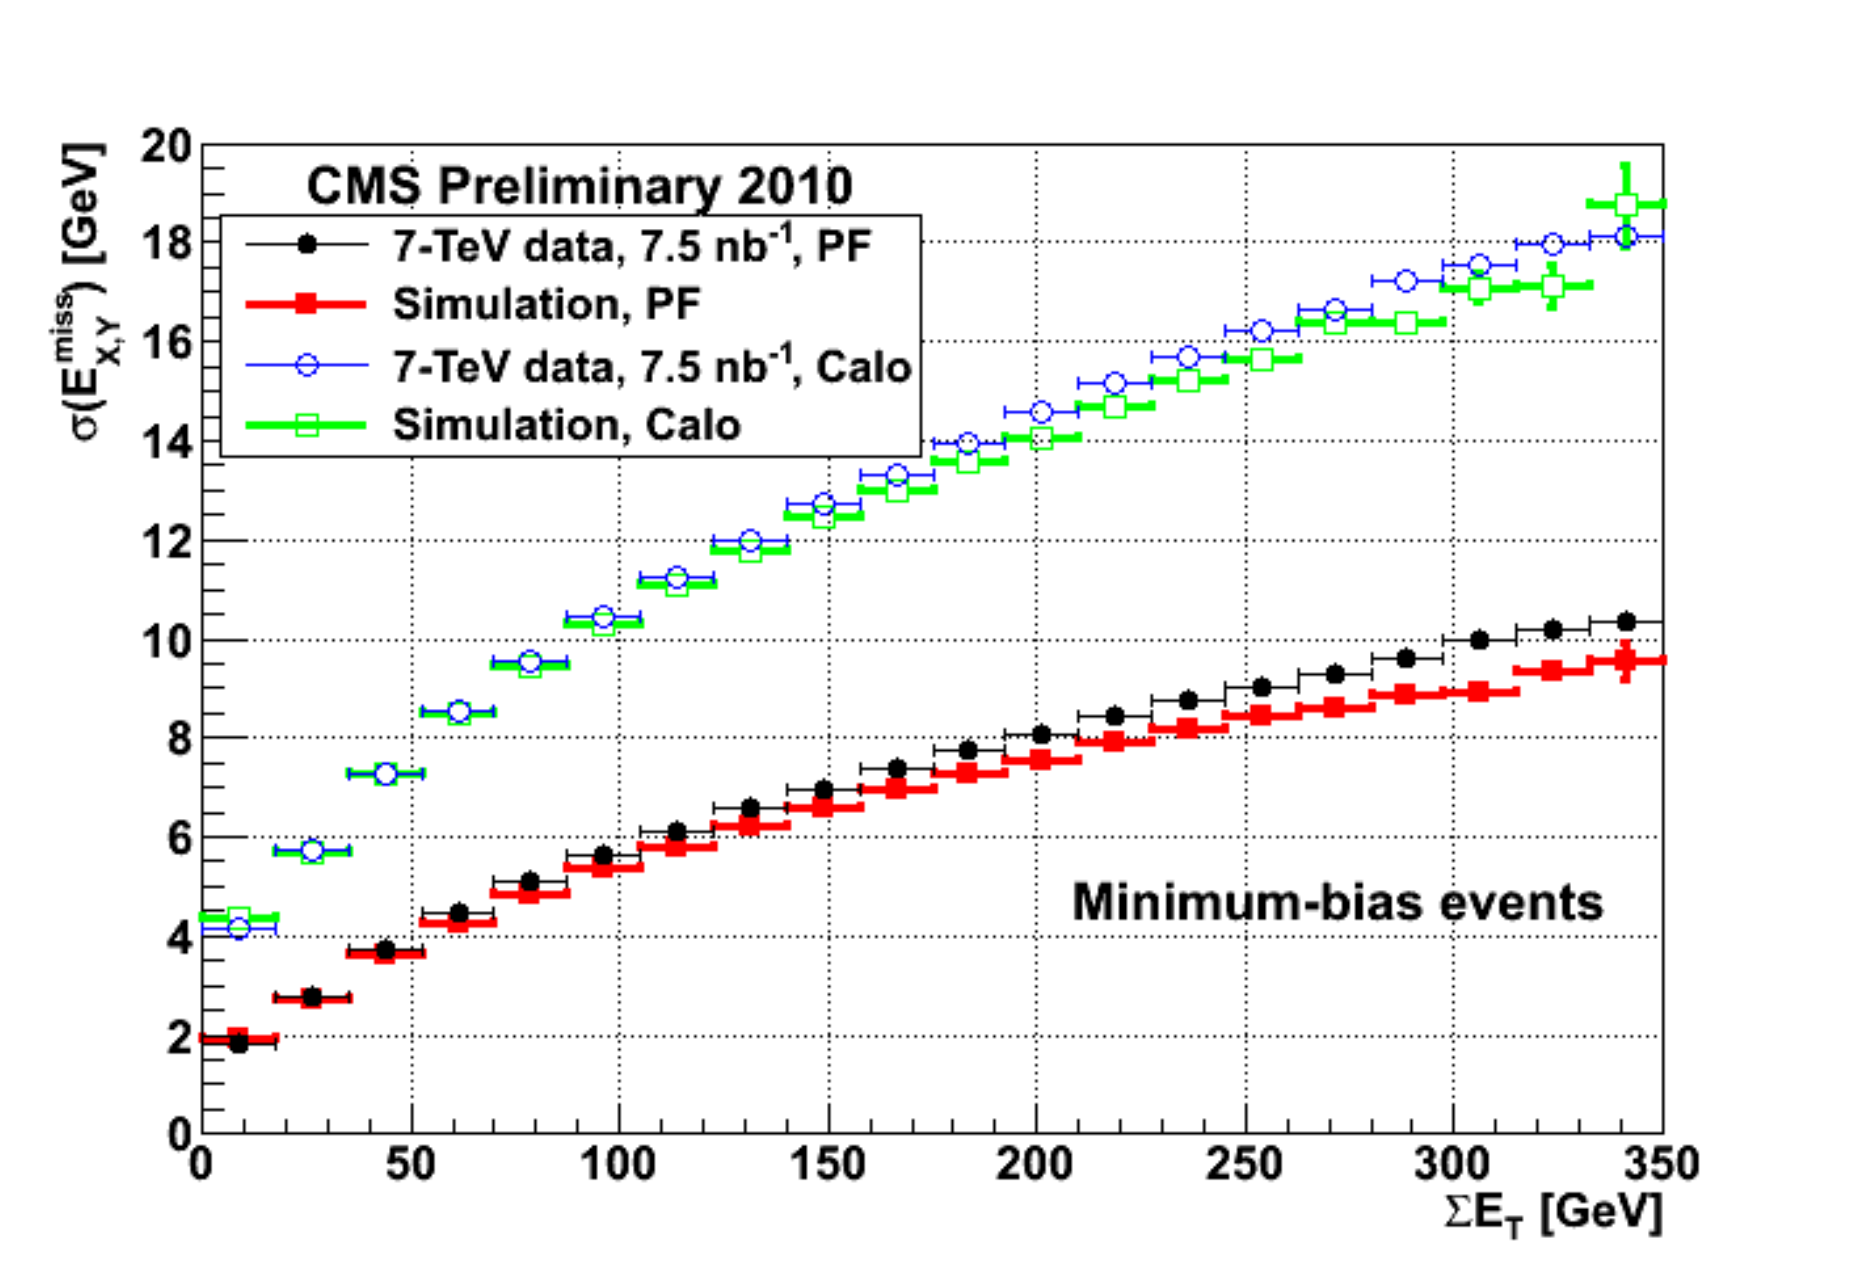
\includegraphics[width=0.7\textwidth]{chapitre3/figs/pf_met_resolution.png}
    \caption{Résolution de l'énergie transverse manquante \emph{particle-flow} et calorimétrique en fonction de la somme scalaire de l'énergie transverse de toutes les particules dans l'événement ($\sum E_T$), obtenue sur les données 2010. \citep{cms_pf_jets}.}
    \label{fig:met_resolution}
\end{figure}

Par définition, les collisions au sein de CMS se déroulent le long de l'axe $z$. L'impulsion dans le plan ($x$, $y$) est donc nulle. Par conservation de l'impulsion, ce bilan doit rester nul après reconstruction de l'événement : un bilan non nul signifie que des particules n'ont pas été correctement reconstruites. C'est par exemple le cas des neutrinos, qui n'interagissent que très peu avec la matière, et ne sont par conséquent jamais détectés.

Afin de quantifier cette perte d'énergie, on introduit le vecteur énergie transverse manquante. La norme de ce vecteur est communément appelée énergie transverse manquante (MET), symbolisée par \met. A l'aide de l'algorithme de \emph{particle-flow}, on définit le vecteur énergie transverse manquante comme l'opposé de la somme vectorielle des impulsions transverses de toutes les particules de l'événement. La résolution sur la mesure de \met est très importante, puisque de nombreux modèles de nouvelle physique prédisent des particules qui interagissent peu voire pas avec la matière : l'énergie manquante est alors le seul moyen de pouvoir les mettre en évidence. On présente \cref{fig:met_resolution} la résolution de \met reconstruite grâce au \emph{particle-flow}, obtenue sur les données 2010. À titre de comparaison, la résolution de \met reconstruite seulement à l'aide des dépôts calorimétriques (calomet) est aussi présentée dans la même figure.

\section{Conclusion}

On a pu voir au cours de ce chapitre combien il est important de posséder une chaine de simulation complète et performante. Dans un premier temps, il faut être capable de générer correctement un processus physique. Cette étape est réalisée par les générateurs d'événements à éléments de matrice, ainsi que par les générateur à gerbe partonique. Il est ensuite nécessaire de simuler de façon précise la réponse du détecteur. Cette étape est cruciale, et impose une excellente connaissance du détecteur : des progrès sont continuellement réalisés afin d'améliorer la simulation. Enfin, le processus de reconstruction des objets physiques, commun à la simulation et aux données collectées, est capital pour les analyses de physique. CMS dispose de puissants outils de reconstruction. À l'aide de l'algorithme du \pf, tous les sous-détecteurs sont utilisés pour la reconstruction des objets physique, ce qui permet d'améliorer sensiblement la résolution des objets reconstruits. On dispose également d'algorithmes performants pour la reconstruction des jets, primordial dans un environnement hadronique où un grand nombre de jets sont produits.

\medskip

Le prochain chapitre est dédié aux corrections en énergie appliquées aux jets, en insistant particulièrement sur le dernier niveau de correction, qui fût l'un des travaux que j'ai effectué durant ma thèse.
\cleardoublepage\chapter{Correction en énergie des jets à l'aide d'événements \texorpdfstring{$\Pphoton$}{γ} + jets} \label{chap:jetmet}

\begin{fmffile}{chapitre4}

Comme on a pu le voir au chapitre précédent, les algorithmes de reconstruction des jets sont complexes : ils opèrent sur une liste d'objets et les agglomèrent s'ils respectent certaines conditions (voir \cref{sec:jet_reco}). Les propriétés du jet (énergie, impulsion, charge, etc.) sont ainsi déterminées grâce à ces constituants. Ainsi, s'il en manque certains, ou si leurs énergies sont mal déterminées, les propriétés du jet seront impactées.

\smallskip

C'est pourquoi on applique aux jets toute une série de corrections, destinées à corriger ces effets. Les différentes étapes de correction sont détaillées dans ce chapitre.

\section{Les différents niveaux de correction}

Plusieurs effets sont à prendre en compte lorsque l'on veut corriger l'énergie des jets. En effet, la réponse des sous-détecteurs peut varier selon plusieurs facteurs, tels que la présence de \pu, la position angulaire et l'impulsion transverse des particules, le type de particule, ...

CMS a adopté une approche factorisée afin de corriger convenablement ces effets. Plusieurs niveaux de corrections sont ainsi définis, chacun corrigeant un effet particulier. Chaque niveau dépend des corrections appliquées au niveau précédent, et l'ordre dans lequel sont appliquées ces corrections est donc important. On compte trois niveaux de corrections différents :

\begin{description}
    \item[Niveau 1] Ce niveau de correction corrige les effets du \pu et du bruit des détecteurs.
    \item[Niveau 2 et 3] Ces niveaux permettent de corriger les variations d'efficacité de la reconstruction des jets, en fonction de l'angle et l'impulsion transverse des jets.
\end{description}

Ces corrections sont appliquées à la fois aux données collectées et à la simulation. Néanmoins, il est apparu que la simulation ne reproduisait pas (encore) parfaitement la réalité. Il a donc été décidé d'ajouter un quatrième niveau de correction, nommé corrections résiduelles, appliqué uniquement aux données, qui permet de corriger des dernières différences qui subsistent entre données et simulation.

\medskip

Chaque niveau est décrit en détails ci-dessous.

\subsection[Les corrections de niveau 1]{Les corrections de niveau 1 \citep{1748-0221-6-11-P11002}} \label{sec:jec_l1}

On a déjà vu lors du \cref{chap:detecteur} que le \pu entraînait une activité supplémentaire dans le détecteur. Cela se traduit directement par une augmentation de l'énergie des jets reconstruits, puisque certaines particules agglomérées au sein d'un jet proviennent en réalité des interactions parasites plutôt que de l'événement dur.

\medskip

Grâce à l'algorithme du \pf, il est possible de réduire l'impact du \pu sur la reconstruction des jets en appliquant un filtre spécial chargé d'éliminer les hadrons chargés provenant des interactions secondaires. On a en effet vu \cref{sec:pileup} que le \pu venait des collisions parasites d'autres protons. Pour les particules chargées, il est possible d'utiliser le trajectographe pour déterminer très précisément la position des vertex d'interaction. Seules les particules provenant du vertex primaire sont intéressantes. On élimine ainsi les hadrons chargés provenant des vertex de \pu.

Ce n'est cependant pas suffisant pour totalement supprimer la contribution du \pu, puisque environ \SI{40}{\%} de l'énergie d'un jet provient de hadrons neutres ou de photons (voir \cref{fig:pf_jets_composition}).

\bigskip

Tous les jets ne sont pas sensibles de la même façon au \pu. On estime la fraction d'énergie de chaque jet due au \pu en calculant la densité d'énergie $\rho$ par unité de surface, qui caractérise l'activité des jets du \pu. Pour ce faire, on utilise l'aire des jets ($A$), définie comme l'étalement du jet dans le plan $\eta - \phi$. La densité $\rho$ est alors définie comme la médiane de la distribution $p_T^j / A_j$, où $j$ est l'index d'un jet dans l'événement.

On corrige ainsi événement par événement et jet par jet la contribution du \pu en appliquant un facteur de correction $C$ donné par
\begin{align*}
  C &= 1 - \frac{(\rho - \rho_0) \, \beta(\eta) \, A_j}{p_T^{\text{non corrigé}}}
\end{align*}
où $\rho_0$ est la contribution à la densité d'énergie de l'événement sous-jacent et du bruit électronique, mesurée dans des événements avec une seule interaction (sans \pu), et $\beta$ un facteur de correction dépendant de $\eta$, qui permet de tenir compte de la non uniformité de la mesure de la densité d'énergie $\rho$ en $\eta$.

% Deux méthodes sont employées dans CMS afin de supprimer la contribution du \pu : la méthode \emph{offset} et la méthode \emph{fastjet} \citep{l1fastjet_1,l1fastjet_2}. La méthode \emph{fastjet} est maintenant standard dans CMS, et repose sur la méthode \emph{offset}.

% \begin{figure}
%   \subcaptionbox{\label{fig:l1_offset}}[0.45\textwidth]{\includegraphics[width=0.45\textwidth]{chapitre4/figs/l1_offset.pdf}} \hfill
%   \subcaptionbox{\label{fig:l1_offset_vs_fastjet}}[0.45\textwidth]{\includegraphics[width=0.45\textwidth]{chapitre4/figs/l1_offset_vs_fastjet.pdf}} \hfill
%   \caption{(\subref{fig:l1_offset}) \emph{offset} en fonction du nombre de vertex, pour $\num{2} < \aeta < \num{2.1}$, calculé sur des événements multi-jets simulés. (\subref{fig:l1_offset_vs_fastjet}) comparaison entre les méthodes \emph{offset} et \emph{fastjet}.}
%   \label{fig:jec_l1}
% \end{figure}

% \subsubsection{La méthode \emph{offset}}

% Des événements de biais minimum\footnote{Un événement de biais minimum est un événement représentatif d'une collision \Pproton{}\Pproton} sont utilisés afin d'estimer l'énergie moyenne portée par un jet à cause du \pu. \fxnote{dire pourquoi du min  bias} Cette énergie moyenne est déterminée en fonction du nombre de vertex ($N_{PV}$), ainsi qu'en fonction de $\aeta$ (voir \cref{fig:l1_offset}). On obtient ainsi une correction dépendante du nombre de vertex, ainsi que de \aeta. Cette correction est à soustraire de l'énergie du jet afin de supprimer la contribution du \pu.

% \subsubsection{La méthode \emph{fastjet}}

% Il s'avère que tous les jets ne portent pas la même énergie due au \pu. La méthode \emph{fastjet} améliore ainsi la méthode \emph{offset} en ajoutant une dépendance des corrections en fonction de l'aire des jets ($A$) et en fonction de la densité d'énergie ($\rho$), définie comme la médiane de la distribution $p_T^j / A_j$, où $j$ est l'index d'un jet dans l'événement. La correction obtenue est donc dépendante de $\rho$, de $A$ et de \aeta. On présente \cref{fig:l1_offset_vs_fastjet} une comparaison entre ces deux méthodes.

\begin{figure}
  \subcaptionbox{\label{fig:l1_no_corr}}[0.45\textwidth]{\includegraphics[width=0.45\textwidth]{chapitre4/figs/l1_effect_no_corr.pdf}} \hfill
  \subcaptionbox{\label{fig:l1_with_corr}}[0.45\textwidth]{\includegraphics[width=0.45\textwidth]{chapitre4/figs/l1_effect_with_corr.pdf}} \hfill
  \caption{Évolution de la réponse des jets en fonction de l'impulsion transverse simulée, avant l'application des corrections de niveau 1 (\subref{fig:l1_no_corr}) et après (\subref{fig:l1_with_corr}), pour différentes classes de $N_{PV}$.}
  \label{fig:jec_l1_effect}
\end{figure}

\bigskip

Après application des corrections de niveau 1, la réponse des jets, définie comme le rapport en l'impulsion transverse du jet sur l'impulsion transverse vraie\footnote{L'impulsion transverse vraie d'un jet est la valeur de l'impulsion transverse dans le cas où le jet est parfaitement reconstruit. Cette valeur est déterminée en agglomérant les particules directement en sortie du générateur, plutôt que les particules après reconstruction.}, n'est plus dépendante du nombre de vertex primaires, comme on peut le voir \cref{fig:jec_l1_effect}.

\subsection[Les corrections de niveau 2 et 3]{Les corrections de niveau 2 et 3 \citep{1748-0221-6-11-P11002}} \label{sec:jec_l2l3}

Les corrections de niveau 2 (corrections en fonction de \aeta) et de niveau 3 (corrections en fonction de \pt) sont appliquées après celles de niveau 1. Ces deux niveaux de corrections forment en réalité une correction unique, la séparation en deux niveaux distincts étant purement historique.

Après les corrections de niveau 1, la réponse n'est plus dépendante du \pu. Néanmoins, elle varie toujours en fonction de \aeta et du $p_T$. On corrige cette dépendance grâce à la simulation.

\begin{figure}[tbp]
    \centering
    \subcaptionbox{\label{fig:resp_l1l2l3}}[0.45\textwidth]{\includegraphics[width=0.45\textwidth]{chapitre4/figs/response_after_l1l2l3.pdf}} \hfill
    \subcaptionbox{\label{fig:jet_flavor_resp}}[0.45\textwidth]{\includegraphics[width=0.45\textwidth]{chapitre4/figs/jet_flavor_response.pdf}} \hfill
    \caption{(\subref{fig:resp_l1l2l3}) Réponse des jets après application des corrections de niveau 1, 2 et 3, pour des événements multi-jets simulés. (\subref{fig:jet_flavor_resp}) Différence de réponse entre les jets légers (\Pup, \Pdown, \Pstrange), les jets de gluons, les jets de \Pcharm et les jets de \Pbottom.}
\end{figure}

\smallskip

On utilise des événements multi-jets pour déterminer les facteurs de corrections à appliquer. On réalise une grille 2D en $\eta$ et en $p_T$, et, pour chaque classe, on détermine la réponse des jets définie comme
\begin{align*}
  R &= \dfrac{p_T}{p_T^\text{vrai}}
\end{align*}
où $p_T^\text{vrai}$ est l'impulsion transverse du jet généré à partir des particules MC (impulsion transverse vraie). Le facteur de correction est alors $1 / R$, et dépend à la fois de $\eta$ et de $p_T$.


%Afin de corriger ces effets, on utilise des événements di-jets. Par conservation de l'impulsion transverse, on a donc $p_T^\text{jet 1} = p_T^\text{jet 2}$. De plus, on considère que les jets dans la région centrale du détecteur ($\aeta < \num{1.3}$) sont correctement reconstruit. On sélectionne donc des événements avec au moins un jet dans la région centrale, et on calcule la réponse $R$, définie comme $p_T^\text{jet} / p_T^\text{central}$, en fonction de \aeta et $p_T$. Dans le cas d'une reconstruction parfaite, la réponse vaut 1. Dans le cas contraire, le facteur de correction à appliquer est $1 / R$.

%\begin{figure}
  %\subcaptionbox{\label{fig:l2l3_response}}[0.45\textwidth]{\includegraphics[width=0.45\textwidth]{chapitre4/figs/l2l3_response.pdf}} \hfill
  %\subcaptionbox{\label{fig:l1l2l3}}[0.45\textwidth]{\includegraphics[width=0.45\textwidth]{chapitre4/figs/response_after_l1l2l3.pdf}} \hfill
  %\caption{Évolution de la réponse des jets en fonction de l'impulsion transverse simulée, avant l'application des corrections de niveau 1 (\subref%{fig:l1_no_corr}) et après (\subref{fig:l1_with_corr}), pour différentes classes de $N_{PV}$.}
%  \label{fig:jec_l2l3}
%\end{figure}

\bigskip

On présente \cref{fig:resp_l1l2l3} la réponse des jets après application des corrections de niveau 1, 2 et 3, pour des événements multi-jets simulés. La réponse est linéaire, c'est-à-dire indépendante de $p_T$, et vaut maintenant 1. La dépendance en $\eta$ est aussi supprimée lors de l'application des corrections de niveau 2 et 3.

\bigskip

Ces facteurs de corrections ont été déterminés sur des événements multi-jets, très riches en jets de gluons. Cependant, on peut voir \cref{fig:jet_flavor_resp} que la réponse du jet dépend de sa saveur. Pour l'instant, cette différence de réponse est prise en compte aux travers des erreurs systématiques, et on verra plus loin dans ce chapitre que des études sont menées par CMS afin de déterminer des corrections aussi dépendantes de la saveur des jets.

\subsection[Les corrections résiduelles]{Les corrections résiduelles \citep{1748-0221-6-11-P11002}} \label{sec:jec_res}

Les corrections précédentes sont toutes dérivées à l'aide de la simulation. Malheureusement, cette simulation n'est pas parfaite, et des différences existent entre la réponse des jets dans la simulation et dans les données collectées. On applique ainsi un autre niveau de corrections, uniquement sur les données, afin de corriger des dernières différences entre données et simulation. Ces corrections, dépendantes de \aeta et du $p_T$ des jets, sont déterminées à l'aide d'événements $\PZ \rightarrow \left[ \Pmuon \APmuon \, | \, \Pelectron \APelectron \right] $ + jets ou $\Pphoton$ + jets, ainsi que des événements di-jets pour la dépendance en \aeta.

La détermination des corrections résiduelles à l'aide d'événement $\Pphoton$ + jets est décrite en détail dans la \cref{sec:jetmet_gamma_jet}.

\subsection{Erreurs systématiques} \label{sec:jec_uncertainties}

Face à la complexité de la détermination des corrections des jets, l'erreur systématique associée est souvent l'erreur dominante dans les analyses de physique, atteignant souvent des valeurs proches de \SI{10}{\%}. Beaucoup d'efforts sont faits pour améliorer notre compréhension des détecteurs et ainsi réduire ces erreurs systématiques.

\medskip

On trouve \cref{fig:jetmet_uncertainties} l'évolution des erreurs systématiques en fonction de \pt (\cref{fig:uncertainties_vs_pt}) et en fonction de \aeta (\cref{fig:uncertainties_vs_eta}). Cette erreur se décompose en 6 sources indépendantes :

\begin{figure}[tbp]
    \centering
    \subcaptionbox{\label{fig:uncertainties_vs_pt}}[0.45\textwidth]{\includegraphics[width=0.45\textwidth]{chapitre4/figs/uncertainties/uncertainties_vs_pt.pdf}} \qquad
    \subcaptionbox{\label{fig:uncertainties_vs_eta}}[0.45\textwidth]{\includegraphics[width=0.45\textwidth]{chapitre4/figs/uncertainties/uncertainties_vs_eta.pdf}}
    \caption{Erreurs systématiques associées aux corrections des jets en fonction de \pt (\subref{fig:uncertainties_vs_pt}) pour $\aeta \simeq 0$, et en fonction de \aeta (\subref{fig:uncertainties_vs_eta}) pour $\pt = \SI{100}{\GeV}$.}
    \label{fig:jetmet_uncertainties}
\end{figure}

\begin{itemize}
  \item Les erreurs systématiques liées à la détermination des corrections résiduelles (\emph{absolute scale} et \emph{relative scale}).
  \item Les méthodes employées pour déterminer les corrections résiduelles ne permettent pas d'aller à très bas / haut $p_T$. Une extrapolation est alors réalisée, en se basant sur les résultats obtenus à bas $p_T$. Une erreur systématique est associée à cette procédure (\emph{extrapolation}).
  \item Une erreur systématique liée à la modélisation du \pu (\pu).
  \item La différence de réponse liée à la saveur des jets est prise en compte à travers une erreur systématique dédiée (\emph{jet flavor}).
  \item Les conditions de reconstruction et de calibration du détecteur ont changé pendant la prise de données 2012. Ces différences n'ont pas été propagées à la simulation, et on voit apparaitre des différences de réponse en fonction de la date de la prise de données. Ces différences sont prises en compte \emph{via} une erreur systématique (\emph{time stability}).
\end{itemize}

On constate que la présence de \pu (ligne bleue) contribue en majorité à l'incertitude totale à bas \pt, alors que l'extrapolation devient dominante à haut \pt. De nouvelles techniques de suppression du \pu au niveau 1 sont ainsi en cours de développement, afin de réduire cette erreur systématique. Néanmoins, pour des jets de \SI{100}{\GeV} dans le tonneau ($\aeta < \num{1.3}$), l'erreur systématique totale est inférieure à \SI{2}{\%}.

\section{Détermination des corrections résiduelles à l'aide d'événements \texorpdfstring{$\Pphoton$}{γ} + jets} \label{sec:jetmet_gamma_jet}

\subsection{Intérêt des événements \texorpdfstring{$\Pphoton$}{γ} + jets}

L'application des corrections résiduelles permet de corriger les dernières différences de réponse entre la simulation et les données collectées, après calibrations de niveau 1, 2 et 3. Pour cela, on mesure la réponse des jets à la fois dans les données et dans la simulation, et on corrige les données de la différence de réponse, afin de faire en sorte que la réponse dans les données et dans la simulation soit identique. Il est donc nécessaire d'utiliser un processus physique qui permet de connaître de façon la plus précise possible l'énergie d'un jet, sans avoir à utiliser la vérité de la simulation.

\begin{figure}[t!] \centering
  \subcaptionbox{\label{fig:g_plus_jet_1}}[.4\linewidth]{
  \begin{fmfgraph*}(180,120)
    \fmfpen{0.5}
    \fmfleft{i1,i2}
    \fmfright{o1,o2}
    \fmf{gluon}{i1,v1}
    \fmf{fermion}{i2,v1}
    \fmf{fermion,label=\Pquark}{v1,v2}
    \fmf{fermion}{v2,o1}
    \fmf{photon}{v2,o2}
    \fmffreeze
    \fmfdot{v1,v2}
    \fmflabel{\Pquark}{i2}
    \fmflabel{\Pquark}{o1}
    \fmflabel{\Pphoton}{o2}
  \end{fmfgraph*}}\qquad \quad%
  % \begin{fmfgraph*}(180,120)
  %   \fmfpen{0.5}
  %   \fmfleft{i1,i2}
  %   \fmfright{o1,o2,o3}
  %   \fmf{gluon}{i2,v1}
  %   \fmf{gluon}{v3,o1}
  %   \fmf{fermion}{i1,v3}
  %   \fmf{fermion,label=\APquark}{v3,v2,v1}
  %   \fmf{fermion}{v1,o3}
  %   \fmffreeze
  %   \fmf{photon,label=\Pphoton}{v2,o2}
  %   \fmfdot{v1,v2,v3}
  %   \fmflabel{\Pquark}{i1}
  %   \fmflabel{\Pquark}{o3}
  % \end{fmfgraph*}}\qquad \quad%
  \subcaptionbox{\label{fig:g_plus_jet_2}}[.4\linewidth]{
  % \begin{fmfgraph*}(180,120)
  %   \fmfpen{0.5}
  %   \fmfstraight
  %   \fmfleft{i1,i2}
  %   \fmfright{o1,o2,o3}
  %   \fmf{fermion}{i1,v1,i2}
  %   \fmf{fermion}{v4,v2}
  %   \fmf{phantom}{o1,v4}
  %   \fmf{fermion,label=\Pquark}{v2,v3}
  %   \fmf{photon,label=$\Pphoton$}{v3,o3}
  %   \fmf{gluon}{v1,v2}
  %   \fmffreeze
  %   \fmf{fermion}{v3,o2}
  %   \fmfdot{v1,v2,v3}
  %   \fmflabel{\APquark}{i2}
  %   \fmflabel{\Pquark}{i1}
  %   \fmflabel{\Pquark}{o2}
  %   \fmflabel{\APquark}{v4}
  % \end{fmfgraph*}
  \begin{fmfgraph*}(180,120)
    \fmfpen{0.5}
    \fmfstraight
    \fmfleft{i1,i2}
    \fmfright{o1,o2,o3}
    \fmf{fermion}{i2,v3}
    \fmf{fermion,label=\APquark}{v3,v2}
    \fmf{gluon}{i1,v1,o1}
    \fmf{gluon}{v2,v1}
    \fmf{photon}{v3,o3}
    \fmffreeze
    \fmf{fermion}{v2,o2}
    \fmflabel{\Pquark}{i2}
    \fmflabel{\Pquark}{o2}
    \fmflabel{\Pphoton}{o3}
  \end{fmfgraph*}
  }
  \caption{Exemples de diagrammes de Feynman associés à la production d'un photon et d'un jet (\subref{fig:g_plus_jet_1}) et d'un photon et de deux jets (\subref{fig:g_plus_jet_2}).}
  \label{fig:gamma_jet_diagrams}
\end{figure}

On utilise pour cela des processus comportant uniquement deux particules dans l'état final : une particule dont on connaît très bien les propriétés (boson \PZ, photon, \ldots), qui sera notre sonde, et un jet. On utilise ensuite les propriétés de la sonde pour déterminer celles du jet. Par la suite, seuls les événements \Pphoton + jets seront abordés.

\bigskip

On présente \cref{fig:gamma_jet_diagrams} deux diagrammes de Feynman représentant la production d'un photon accompagné d'un ou deux jets. L'impulsion dans le plan transverse étant nulle au moment de la collision, on a dans l'état final
\begin{align*}
  \vec{p}_T &= 0 = \vec{p}_{T}^{\Pphoton} + \vec{p}_T^\text{jet}\\
  \norm{\vec{p}_T^{\Pphoton}} &= \norm{\vec{p}_T^{\text{jet}}}
\end{align*}

Ainsi, il est suffisant de connaître l'impulsion transverse de la sonde pour déterminer l'impulsion transverse du jet. L'utilisation du photon comme sonde comporte certains avantages :
\begin{itemize}
  \item Comme on a déjà pu le voir lors du \cref{chap:reco}, le calorimètre électromagnétique est bien plus performant que le calorimètre hadronique. La résolution sur la reconstruction des photons est \tilde\SI{2}{\%}, contre \tilde{10}{\%} pour les jets.
  \item Comparé à d'autres processus comme \PZ + jets, la section efficace de production \Pphoton + jets au LHC à \SI{8}{\TeV} est bien plus grande : le nombre d'événements disponible est ainsi plus important.
  \item La production d'événements \Pphoton + jets n'est pas résonante, à la différence des événements \PZ + jets. Il est ainsi possible d'explorer une gamme en impulsion transverse beaucoup plus large.
\end{itemize}

\subsection{Détermination de la réponse des jets}

% On cherche à déterminer la réponse $R$ des jets, qui tend vers 1 si l'on reconstruit parfaitement le jet. On utilise deux méthodes différentes pour déterminer cette réponse : la méthode de la balance et la méthode MPF, détaillées ci-dessous.

Deux méthodes différentes sont utilisées afin de déterminer la réponse $R$ des jets : la méthode de la balance et la méthode MPF, détaillées ci-dessous.

\subsubsection{La méthode de la balance}

On utilise le principe de conservation de l'impulsion transverse. Pour un événement où le photon est parfaitement équilibré avec le jet dans le plan transverse, on a
\begin{align*}
  \norm{\vec{p}_T^{\Pphoton}} &= \norm{\vec{p}_T^{jet}}
\end{align*}
et on définit la réponse $R$ par la relation
\begin{align*}
    R &= \frac{p_T^\text{jet}}{p_T^{\Pphoton}}
\end{align*}

Cette méthode est très simple et performante. Néanmoins, elle est très sensible au \pu, ainsi qu'aux radiations dans l'état final. En effet, la présence d'autres jets dans l'état final vont venir perturber la balance entre le jet et le photon. Il est cependant possible de restaurer cet équilibre, en utilisant une extrapolation.

\paragraph{L'extrapolation}

La balance entre le photon et le jet est perturbée par la présence de jets additionnels dans l'événement, provenant de radiations dans l'état final. On définit $\alpha$ comme le rapport entre l'impulsion transverse du second jet de l'événement et l'impulsion transverse du photon,
\begin{align*}
    \alpha &= \frac{p_T^{\text{\ordinalnum{2} jet}}}{p_T^\gamma}
\end{align*}

Afin de réduire l'influence des jets additionnels sur la réponse, on effectue un découpage de la réponse en $\alpha$, et on extrapole le comportement de la réponse pour $\alpha \rightarrow 0$.

\subsubsection{La méthode MPF (\emph{Missing $E_T$ projection fraction})} \label{sec:mpf}

Un événement \Pphoton + jets n'a pas d'énergie transverse manquante. Ainsi, au niveau partonique, on a
\begin{align*}
  \vec{p}_T^{\Pphoton} + \vec{p}_T^{\text{recul}} &= -\vec{\met} = \vec{0}
\end{align*}
où $\vec{p}_T^{\text{recul}}$ est le vecteur impulsion transverse de toutes les particules dans l'événement différentes du photon.

Après reconstruction, on a
\begin{align*}
  R_{\Pphoton} \, \vec{p}_T^{\Pphoton} + R_{\text{recul}} \, \vec{p}_T^{\text{recul}} &= -\vec{\met}
\end{align*}
$R_X$ désigne ici la réponse des détecteurs lors de la reconstruction de l'objet $X$.

On considère que les photons sont reconstruits de façon parfaite, on pose donc $R_{\Pphoton} = 1$. En utilisant le fait que $\vec{p}_T^{\text{recul}} = -\vec{p}_T^{\Pphoton}$ on obtient
\begin{align*}
  R_{\text{recul}} &= 1 + \frac{\vec{\met} \cdot \vec{p}_T^{\Pphoton}}{\left( p_T^{\Pphoton} \right)^2} \equiv R_{\text{MPF}}
\end{align*}

À la différence de la méthode de la balance, cette méthode n'est pas dépendante de la présence de jets additionnels dans l'événement, mais requiert par contre une excellente reconstruction de l'énergie transverse manquante. C'est le cas dans CMS grâce à l'utilisation de l'algorithme du \pf.

\medskip

Cette méthode est utilisée pour produire les corrections officielles. La méthode de la balance permet de vérifier la compatibilité des corrections obtenues.

\end{fmffile}

\subsection{Sélection des événements} \label{sec:jetmet_sel}

Pour déterminer les corrections résiduelles, on sélectionne sur les données des événements contenant un unique photon, ainsi qu'un ou deux jets. Le principal bruit de fond est dû aux événements multi-jets où un jet est incorrectement identifié comme un photon. On étudie les performances de notre sélection sur des événement \Pphoton + jets simulés, considérés comme notre signal, ainsi que sur des événements multi-jets, le bruit de fond.

Afin d'éliminer une grande partie du bruit de fond, une sélection est appliquée. La première étape consiste à sélectionner des événements contenant uniquement un seul photon. On utilise pour cela une méthode d'identification des photons. Suivant les besoin des analyses, cette méthode peut être optimisée pour obtenir une grande efficacité de sélection et une faible pureté (beaucoup d'événements sont sélectionnés, mais certains ne sont pas des vrais photons) ou au contraire une grande pureté et une faible efficacité (moins d'événements sont sélectionnés, mais la probabilité qu'ils ne soient pas de vrais photons est très faible).

On souhaite obtenir les événements les plus purs possibles. On choisit donc le point de fonctionnement offrant la plus grande pureté (\tilde\SI{96}{\%} des photons sont des vrais photons), mais une efficacité plus faible ($\tilde \SI{70}{\%}$). Cette identification est définie de la façon suivante :

\begin{enumerate}
    \item Un contrôle est effectué pour vérifier que le photon n'est pas en réalité un électron dont la trace n'a pas pu être liée au dépôt calorimétrique, et qu'il ne provient pas du rayonnement bremsstrahlung d'un électron lors de son passage dans le ECAL.
    \item Le ratio entre l'énergie collectée dans le calorimètre hadronique et l'énergie collectée dans le calorimètre électromagnétique doit être inférieur à \SI{5}{\%}. La majorité de l'énergie doit donc être déposée dans le calorimètre électromagnétique.
    \item $\sigma_{i\eta i\eta} < \num{0.011}$. Cette variable représente la largeur de l'agrégat calorimétrique en \aeta, et est caractéristique de la forme de la gerbe électronique dans le calorimètre électromagnétique, plus étalée dans le cas d'un électron que d'un photon.
\end{enumerate}

En plus de ces trois critères, on demande que le photon soit isolé. On définit l'isolation $I$ comme le rapport entre l'énergie de toutes les particules \pf contenues dans un cône de rayon $\Delta R = \num{0.3}$ centré autour du photon et l'énergie du photon. Cette valeur étant hautement sensible au \pu, on applique une procédure qui permet de diminuer son impact, en corrigeant cette isolation par un facteur dépendant de la densité d'énergie $\rho$. On a ainsi $I_\text{corr} = \max{\left(I - f(\rho), 0\right)}$. On effectue des coupures sur cette isolation selon trois différents types de particules : les hadrons neutres, chargés, et les photons :

\begin{itemize}
    \item $I_\text{hadrons neutres} < \num{0.4} + \num{0.04} \, p_T^{\Pphoton}$
    \item $I_\text{hadrons chargés} < \num{0.7}$
    \item $I_\text{photons} < \num{0.5} + \num{0.005} \, p_T^{\Pphoton}$
\end{itemize}

Afin de ne garder que les photons les mieux reconstruits, on sélectionne uniquement ceux reconstruits dans le tonneau, avec $\aeta < \num{1.3}$, et une impulsion transverse d'au moins \SI{40}{\GeV}.

\medskip

\begin{figure}[tbp] \centering
  \subcaptionbox{\label{fig:schema_gamma_jet}}[0.45\textwidth]{\scalebox{2}{\begin{tikzpicture}[rotate=45]
    \draw[draw=red!50!black,dashed,->] (0:0) -- (95:1.5) ;
    \draw (90:1) node[right] {\tiny $\gamma$} ;

    \draw[draw=blue!60,dashed,->] (0:0) -- (-85:1.7) ;

    \draw[dashed] (95:4mm) arc (90:-80:4mm) ;
    \draw (5:7mm) node {\tiny $\Delta\phi$} ;

    \begin{scope}[rotate=5]
      \fill[top color=blue!50!black,bottom color=blue!10,middle color=blue,shading=axis,opacity=0.25] (0,-13mm) circle (3mm and 1mm);
      \fill[left color=blue!50!black,right color=blue!50!black,middle color=blue!50,shading=axis,opacity=0.25] (3mm,-13mm) -- (0,0mm) -- (-3mm,-13mm) arc (180:360:3mm and 1mm);
      \draw[draw=blue!50!black,opacity=0.25] (-3mm,-13mm) arc (180:360:3mm and 1mm) -- (0,0mm) -- cycle;
      \draw[draw=blue!50!black,opacity=0.25,densely dashed] (-3mm,-13mm) arc (180:0:3mm and 1mm);
    \end{scope}

    \draw (-55:0.9) node {\tiny jet} ;
    \draw (0:0) node {\tiny $\bullet$} ;

  \end{tikzpicture}}} \quad
  \subcaptionbox{\label{fig:schema_gamma_jets}}[0.45\textwidth]{\scalebox{2}{\begin{tikzpicture}
    \draw[draw=red!50!black,dashed,->] (0:0) -- (45:1.5) ;
    \draw (40:1) node[right] {\tiny $\gamma$} ;

    \draw[draw=blue!60,dashed,->] (0:0) -- (-100:1) ;
    \draw[draw=blue!60,dashed,->] (0:0) -- (-162.5:1.7) ;

    \begin{scope}[rotate=-72]
      \fill[top color=blue!50!black,bottom color=blue!10,middle color=blue,shading=axis,opacity=0.25] (0,-13mm) circle (3mm and 1mm);
      \fill[left color=blue!50!black,right color=blue!50!black,middle color=blue!50,shading=axis,opacity=0.25] (3mm,-13mm) -- (0,0mm) -- (-3mm,-13mm) arc (180:360:3mm and 1mm);
      \draw[draw=blue!50!black,opacity=0.25] (-3mm,-13mm) arc (180:360:3mm and 1mm) -- (0,0mm) -- cycle;
      \draw[draw=blue!50!black,opacity=0.25,densely dashed] (-3mm,-13mm) arc (180:0:3mm and 1mm);
    \end{scope}

    \begin{scope}[rotate=-10]
      \fill[top color=blue!50!black,bottom color=blue!10,middle color=blue,shading=axis,opacity=0.25] (0,-7mm) circle (2mm and 0.5mm);
      \fill[left color=blue!50!black,right color=blue!50!black,middle color=blue!50,shading=axis,opacity=0.25] (2mm,-7mm) -- (0,0mm) -- (-2mm,-7mm) arc (180:360:2mm and 0.5mm);
      \draw[draw=blue!50!black,opacity=0.25] (-2mm,-7mm) arc (180:360:2mm and 0.5mm) -- (0,0mm) -- cycle;
      \draw[draw=blue!50!black,opacity=0.25,densely dashed] (-2mm,-7mm) arc (180:0:2mm and 0.5mm);
    \end{scope}

    \draw (-84:1) node {\tiny jet} ;
    \draw (-187:1.1) node {\tiny jet} ;
    \draw (0:0) node {\tiny $\bullet$} ;

  \end{tikzpicture}}}
  \caption{Un événement $\gamma$ + jets parfaitement dos-à-dos (\subref{fig:schema_gamma_jet}) et où la balance est brisée (\subref{fig:schema_gamma_jets}).}
  \label{fig:schema_g_jet}
\end{figure}

On demande au moins un jet dans l'événement, reconstruit grâce à l'algorithme anti-$k_T$, avec une largeur de cône $R = \num{0.5}$, composé d'au moins deux particules. Cette identification est très efficace ($> \SI{99}{\%}$) et permet d'éliminer les faux jets dû à des bruits dans les détecteurs. La séparation azimutale $\abs{\Delta \phi}$ dans le plan transverse entre le photon et le premier jet de l'événement doit être supérieure à \SI{2.8}{\radian}, afin de ne conserver que les événements où le photon et le jet sont dos-à-dos. Les \cref{fig:schema_gamma_jet,fig:schema_gamma_jets} représentent un événement $\Pphoton$ + jets avec 1 ou 2 jets. Dans le cas où un second jet est présent, on vérifie que son énergie est inférieure à \SI{20}{\%} de celle du photon ($\alpha < \num{0.20}$), afin d'éviter de conserver des événements trop déséquilibrés. Cette condition n'est appliquée que si $p_T^{\text{\ordinalnum{2} jet}} \geq \SI{10}{\GeV}$. Tous les jets sont corrigés avec les corrections de niveau 1, 2 et 3.

\label{page:met_propagation} Toutes les corrections effectuées sur les jets sont ensuite propagées à l'énergie transverse manquante. En effet, on rappelle que \met est définie comme l'opposé de la somme vectorielle des impulsions transverses de toutes les particules de l'événement. Si jamais l'impulsion d'une particule est modifiée après calcul de \met, il est nécessaire de propager ces modifications afin de garder une définition cohérente de l'énergie transverse manquante. Ainsi, si pour un jet, on procède à la correction suivante :
\begin{align*}
  p_x \rightarrow p_x + \Delta p_x \\
  p_y \rightarrow p_y + \Delta p_y
\end{align*}
la correction à appliquer sur l'énergie transverse manquante est :
\begin{align*}
  \METx^{\text{corr}} &= \METx - \Delta p_x \\
  \METy^{\text{corr}} &= \METy - \Delta p_y
\end{align*}

Pour terminer la sélection, un véto est imposé sur la présence d'électrons ou de muons isolés dans l'événement. Sur des événements de signal simulés, cette sélection a une efficacité de \tilde \SI{20}{\%}, et inférieure à \tilde\SI{1}{‰} sur le bruit de fond.

\bigskip

Sur les données, on demande à ce que les événements aient passé les chemins de déclenchement demandant un photon isolé. Plusieurs de ces chemins existent en fonction de l'impulsion du photon, dont la plupart avec un facteur de \emph{prescale}\footnote{Il arrive que certains chemins de déclenchement laissent passer trop d'événements. Afin d'éviter de surcharger le HLT, on applique un facteur de \emph{prescale}, définit comme l'inverse de la probabilité de garder un événement. Plus ce facteur est grand, moins les événements ont de chance d'être conservés.} différent de 1. Afin de pouvoir comparer les données et la simulation sans être gêné par ce facteur, on applique une coupure supplémentaire sur l'impulsion transverse du photon à \SI{175}{\GeV}. Cette coupure n'est pas appliquée pour déterminer les facteurs de corrections, mais uniquement pour comparer les distributions.

\smallskip

Finalement, la simulation des événements multi-jets et $\gamma$ + jets a été effectuée pendant la prise de données. À cette époque, le profil de \pu n'était pas encore connu précisément, et une estimation de ce profil a été utilisée pour la simulation. On repondère donc le profil de \pu de la simulation pour qu'il corresponde à celui observé sur les données collectées.

\begin{figure}[p]
    \centering
    \subcaptionbox{\label{pt_photon}}[0.45\textwidth]{\includegraphics[width=0.45\textwidth]{chapitre4/figs/ptPhoton_passedID_log.pdf}}\hfill
    \subcaptionbox{\label{pt_first_jet}}[0.45\textwidth]{\includegraphics[width=0.45\textwidth]{chapitre4/figs/ptFirstJet_passedID_log.pdf}}
    \subcaptionbox{\label{pt_second_jet}}[0.45\textwidth]{\includegraphics[width=0.45\textwidth]{chapitre4/figs/ptSecondJet_passedID_log.pdf}}\hfill
    \subcaptionbox{\label{met}}[0.45\textwidth]{\includegraphics[width=0.45\textwidth]{chapitre4/figs/MET_passedID_log.pdf}}
    \caption{Comparaison entre la simulation (histogrammes) et les données (points) de l'impulsion transverse pour le photon (\subref{pt_photon}), pour le premier jet de l'événement (\subref{pt_first_jet}), le second (\subref{pt_second_jet}) ainsi que pour l'énergie transverse manquante (\subref{met}) après sélection. Une coupure additionnelle sur l'impulsion transverse du photon à \SI{175}{\GeV} a été appliquée pour éviter les effets du facteur de \emph{prescale} des différents chemins de déclenchement (plus de détails \cref{sec:jetmet_strategy}). Ces distributions sont normalisées au nombre d'événements dans les données, et la zone hachurée représente les incertitudes.}
    \label{fig:pt_photon_jet}
\end{figure}

\bigskip

On présente \cref{fig:pt_photon_jet} une comparaison entre la simulation et les données pour l'impulsion transverse du photon, du premier jet de l'événement, du second, ainsi que l'énergie transverse manquante. Les distributions sont normalisées au nombre d'événements dans les données, et l'incertitude sur la simulation comprend l'incertitude statistique, l'incertitude sur la luminosité de \SI{2.6}{\%}, ainsi qu'une incertitude de \SI{10}{\%} sur la valeur des sections efficaces de production \Pphoton + jets et multi-jets. On constate quelques désaccords dans les \cref{pt_first_jet,met}. On considère néanmoins que l'accord est suffisant pour notre analyse, puisque aucune erreur systématique n'est présente dans ces distributions, et qu'à aucun moment ces comparaisons ne sont utilisées dans l'analyse.

\subsection{Stratégie d'analyse} \label{sec:jetmet_strategy}

Les événements sélectionnés sont classés suivant l'impulsion transverse du photon et la position angulaire du jet, afin d'augmenter la sensibilité de l'analyse. 14 classes sont définies en impulsion transverse :

\setlength{\columnsep}{0pt}
\begin{multicols}{4}
  \begin{itemize} \setlength{\itemsep}{0.4\itemsep}
      \item 40 - \SI{50}{\GeV}
      \item 50 - \SI{60}{\GeV}
      \item 60 - \SI{75}{\GeV}
      \item 100 - \SI{125}{\GeV}
      \item 125 - \SI{155}{\GeV}
      \item 155 - \SI{180}{\GeV}
      \item 180 - \SI{210}{\GeV}
      \item 250 - \SI{300}{\GeV}
      \item 300 - \SI{350}{\GeV}
      \item 350 - \SI{400}{\GeV}
      \item 400 - \SI{500}{\GeV}
      \item 500 - \SI{600}{\GeV}
      \item 600 - \SI{800}{\GeV}
      \item 800 - \SI{5000}{\GeV}
  \end{itemize}
\end{multicols}

\begin{table} \centering
  \subcaptionbox{Run ACD\label{tab:triggers_runACD}}[0.45\textwidth]{
  \begin{tabular}{@{}cc@{}} \toprule
    Classes en \ptg & Déclencheurs \\ \midrule
    40 - \SI{60}{\GeV} & \texttt{HLT\_Photon30} \\
    60 - \SI{100}{\GeV} & \texttt{HLT\_Photon50} \\
    100 - \SI{155}{\GeV} & \texttt{HLT\_Photon90} \\
    155 - $\inf$ & \texttt{HLT\_Photon135} \\ \bottomrule
  \end{tabular}
  } \qquad
  \subcaptionbox{Run B\label{tab:triggers_runB}}[0.45\textwidth]{
  \begin{tabular}{@{}cc@{}} \toprule
    Classe en \ptg & Déclencheurs \\ \midrule
    40 - \SI{60}{\GeV} & \texttt{HLT\_Photon30} \\
    60 - \SI{100}{\GeV} & \texttt{HLT\_Photon50} \\
    100 - \SI{155}{\GeV} & \texttt{HLT\_Photon90} \\
    155 - \SI{180}{\GeV} & \texttt{HLT\_Photon135} \\
    180 - $\inf$ & \texttt{HLT\_Photon150} \\ \bottomrule
  \end{tabular}}
  \caption{Chemins de déclenchement associés aux classes en \ptg, pour deux périodes de prises de données correspondantes à des conditions de déclenchement différentes.}
  \label{tab:triggers_jetmet}
\end{table}

À \SI{8}{\TeV} et à l'arbre, un processus $\Pphoton$ + 1 / 2 jets a une section efficace de \SI[allow-number-unit-breaks]{99668 \pm 236}{\pb}. À cause de cette section efficace élevée, les chemins de déclenchement demandant simplement un photon possèdent un facteur de \emph{prescale}. Le seul qui ne l'est pas demande ainsi un photon d'au moins \SI{150}{\GeV}. Afin d'éviter tout biais possible dans l'analyse, chaque classe en \ptg{} a été choisie de façon à être associée de façon exclusive à un chemin de déclenchement précis, tout en ayant, si possible, une efficacité de déclenchement maximale. Par exemple, pour la classe 100 - \SI{125}{\GeV}, on demande à ce que l'événement ait déclenché le chemin demandant un photon d'au moins \SI{90}{\GeV} (\texttt{HLT\_Photon90}). Les \SI{10}{\GeV} de différence entre le seuil du déclencheur et la classe en \pt permettent de tenir compte des possibles corrections en énergie entre le photon reconstruit au niveau HLT et le photon \pf. À partir de \SI{155}{\GeV} (ou \SI{180}{\GeV} pour une période spécifique de prise de données), tous les événements doivent déclencher le premier chemin ayant un facteur de \emph{prescale} de 1. Le \cref{tab:triggers_jetmet} résume les chemins de déclenchement associés à chaque classe en \ptg. Les chemins de déclenchement ayant changé pendant la période de prise de données (notamment avec l'apparition puis la disparition du déclencheur \texttt{HLT\_Photon150}), deux tableaux sont présents, un pour chaque période de prise de données.

Les facteurs de \emph{prescale} des chemins de déclenchement vont aussi affecter les distributions de \pu associées. Ainsi, lors de la procédure de repondération du \pu sur la simulation, il faut tenir compte du déclencheur associé à l'événement. En fonction de l'impulsion transverse du photon dans les événements simulés, on détermine quel chemin de déclenchement l'événement aurait dû déclencher sur les données pour passer la sélection, et on utilise cette information pour obtenir le profil de \pu correspondant. On présente \cref{fig:pu_jetmet} une comparaison entre deux profils de \pu, obtenus pour deux chemins de déclenchement différents. On voit très clairement la différence entre les deux profils.

\begin{figure}[tbp]
    \centering
    \includegraphics[width=0.5\textwidth]{chapitre4/figs/pu_plot.pdf}
    \caption{Distribution du nombre moyen d'interactions par croisement de faisceaux pour deux chemins de déclenchement, \texttt{HLT\_Photon30} (rouge) et \texttt{HLT\_Photon150} (bleu)}
    \label{fig:pu_jetmet}
\end{figure}

\bigskip

On procède également à une classification selon $\aeta$ du jet, en 7 classes :

\begin{multicols}{4}
  \begin{itemize} \setlength{\itemsep}{0.4\itemsep}
      \item \num{0} - \num{0.8}
      \item \num{0.8} - \num{1.3}
      \item \num{1.3} - \num{1.9}
      \item \num{1.9} - \num{2.5}
      \item \num{2.5} - \num{3}
      \item \num{3} - \num{3.2}
      \item \num{3.2} - \num{5.2}
  \end{itemize}
\end{multicols}

\begin{figure}[p]
    \centering
    \subcaptionbox{\label{fig:bal_eta013_pt_125_155}}[0.45\textwidth]{\includegraphics[width=0.45\textwidth]{chapitre4/figs/resp_balancing_eta013_ptPhot_125_155.pdf}}\hfill
    \subcaptionbox{\label{fig:bal_eta013_pt_210_250}}[0.45\textwidth]{\includegraphics[width=0.45\textwidth]{chapitre4/figs/resp_balancing_eta013_ptPhot_210_250.pdf}}
    \subcaptionbox{\label{fig:mpf_eta013_pt_125_155}}[0.45\textwidth]{\includegraphics[width=0.45\textwidth]{chapitre4/figs/resp_mpf_eta013_ptPhot_125_155.pdf}}\hfill
    \subcaptionbox{\label{fig:mpf_eta013_pt_210_250}}[0.45\textwidth]{\includegraphics[width=0.45\textwidth]{chapitre4/figs/resp_mpf_eta013_ptPhot_210_250.pdf}}
    \caption{Réponses pour la méthode de la balance (haut) et pour la méthode MPF (bas), pour deux classes en \pt : 125 - \SI{155}{\GeV} (gauche) et 210 - \SI{250}{\GeV} (droite). Pour toutes les distributions, $\aeta < \num{1.3}$. Les histogrammes représentent la simulation et les points les données. La ligne noire correspond à la réponse moyenne $R_m$ extraite sur les données et la ligne bleue celle extraite sur la simulation. Les distributions sont normalisées à la luminosité, et la zone hachurée représente les incertitudes.}
    \label{fig:responses_mpf_balancing}
\end{figure}

Pour chaque classe en $p_T^{\gamma}$ et $\aeta$, on calcule la réponse en utilisant la méthode de la balance et la méthode MPF, sur les données et sur la simulation. On présente \cref{fig:responses_mpf_balancing} les distributions des réponses obtenues pour les deux méthodes, pour diverses classes en \pt, et pour $\aeta < \num{1.3}$. Pour chaque classe, on extrait la réponse moyenne $R_m$, définie comme la moyenne de la distribution des réponses, ainsi que la résolution $\sigma$, définie comme la moyenne quadratique de la distribution des réponses (RMS) divisée par $R_m$. Sur chaque distribution représentée \cref{fig:responses_mpf_balancing}, les réponses moyennes sont représentées par une ligne noire pour les données, et par une ligne bleue pour la simulation. On constate que ces réponses sont différentes, et c'est ce biais que l'on souhaite corriger en appliquant les corrections résiduelles.

\subsection{Résultats} \label{sec:jetmet_results}

Pour chaque distribution des réponses, on extrait la réponse moyenne et la résolution. Afin d'extraire les corrections résiduelles, on trace l'évolution de $R_m$ en fonction de l'impulsion transverse du photon, pour les données et la simulation, pour différentes classes en \aeta. En calculant le rapport entre données et simulation, on détermine le facteur de correction à appliquer sur les données.

On définit le facteur de correction $f$ par
\begin{align*}
  f &= \frac{R_m^{\text{simulation}}}{R_m^{\text{données}}}
\end{align*}

En appliquant ce facteur de correction sur les données, on a
\begin{align*}
  f\;R_m^{\text{données}} &= R_m^{\text{simulation}}
\end{align*}
ce qui est effectivement le but recherché.

\bigskip

On présente par la suite les résultats obtenus avec les méthodes de la balance et MPF, avec et sans extrapolation, qui permettent d'extraire le facteur de correction résiduel. Pour chaque méthode, les distributions des réponses moyennes seront présentées pour différentes classes en \aeta.

\subsubsection{Méthode de la balance, sans extrapolation}

On présente \cref{fig:balancing_resp} les distributions des réponses moyennes pour différentes classes en \aeta. Le ratio entre les données et la simulation accompagne ces distributions, ce qui permet d'extraire les facteurs de corrections. Pour ce faire, une interpolation linéaire par une constante est dérivée à l'aide des divers ratios.
% On trouve aussi \cref{fig:balancing_reso} les distributions des résolutions pour les mêmes classes en \aeta. Même si ces résolutions ne sont pas utilisées pour dériver les corrections résiduelles, elles sont intéressantes pour se rendre compte des performances de reconstruction des algorithmes. On s'aperçoit d'ailleurs que les jets sont mieux reconstruits sur la simulation que sur les données. Cet effet donne lieu à une autre série de corrections pour la résolution, qui vise à dégrader la résolution des jets sur la simulation pour correspondre à celle des données.

\begin{figure}[p]
    \centering
    \subcaptionbox{\label{fig:bal_eta008}}[0.45\textwidth]{\includegraphics[width=0.45\textwidth]{chapitre4/figs/resp_balancing/response_eta008_balancing.pdf}}\hfill
    \subcaptionbox{\label{fig:bal_eta0813}}[0.45\textwidth]{\includegraphics[width=0.45\textwidth]{chapitre4/figs/resp_balancing/response_eta0813_balancing.pdf}}
    \subcaptionbox{\label{fig:bal_eta1319}}[0.45\textwidth]{\includegraphics[width=0.45\textwidth]{chapitre4/figs/resp_balancing/response_eta1319_balancing.pdf}}\hfill
    \subcaptionbox{\label{fig:bal_eta1925}}[0.45\textwidth]{\includegraphics[width=0.45\textwidth]{chapitre4/figs/resp_balancing/response_eta1925_balancing.pdf}}
    \caption{Réponses moyennes pour la méthode de la balance pour $\aeta < \num{0.8}$ (\subref{fig:bal_eta008}), $\num{0.8} \leq \aeta < \num{1.3}$ (\subref{fig:bal_eta0813}), $\num{1.3} \leq \aeta < \num{1.9}$ (\subref{fig:bal_eta1319}), et $\num{1.9} \leq \aeta < \num{2.5}$ (\subref{fig:bal_eta1925}). Le ratio entre les données et la simulation est présenté sous chaque distribution, accompagné d'une interpolation linéaire constante (ligne orange). La bande jaune représente l'erreur sur cette interpolation.}
    \label{fig:balancing_resp}
\end{figure}

% \begin{figure}[p]
%     \centering
%     \subcaptionbox{\label{fig:reso_bal_eta008}}[0.45\textwidth]{\includegraphics[width=0.45\textwidth]{chapitre4/figs/reso_balancing/resolution_eta008_balancing.pdf}}\hfill
%     \subcaptionbox{\label{fig:reso_bal_eta0813}}[0.45\textwidth]{\includegraphics[width=0.45\textwidth]{chapitre4/figs/reso_balancing/resolution_eta0813_balancing.pdf}}
%     \subcaptionbox{\label{fig:reso_bal_eta1319}}[0.45\textwidth]{\includegraphics[width=0.45\textwidth]{chapitre4/figs/reso_balancing/resolution_eta1319_balancing.pdf}}\hfill
%     \subcaptionbox{\label{fig:reso_bal_eta1925}}[0.45\textwidth]{\includegraphics[width=0.45\textwidth]{chapitre4/figs/reso_balancing/resolution_eta1925_balancing.pdf}}
%     \caption{Résolutions pour la méthode de la balance pour $\aeta < \num{0.8}$ (\subref{fig:reso_bal_eta008}), $\num{0.8} \leq \aeta < \num{1.3}$ (\subref{fig:reso_bal_eta0813}), $\num{1.3} \leq \aeta < \num{1.9}$ (\subref{fig:reso_bal_eta1319}), et $\num{1.9} \leq \aeta < \num{2.5}$ (\subref{fig:reso_bal_eta1925}). Le ratio entre les données et la simulation est présenté sous chaque distribution, accompagné d'une interpolation linéaire constante (ligne orange). La bande jaune représente l'erreur sur cette interpolation.}
%     \label{fig:balancing_reso}
% \end{figure}

\begin{table}[p!] \centering
 \begin{tabular}{@{}ccc@{}} \toprule
 Classe en \aeta & ratio & $f$ \\ \midrule
 \num{0} - \num{0.8} & \num{0.966 \pm 0.001} & \num{1.035 \pm 0.001}\\
 \num{0.8} - \num{1.3} & \num{0.957 \pm 0.001} & \num{1.044 \pm 0.001}\\
 \num{1.3} - \num{1.9} & \num{0.958 \pm 0.001} & \num{1.044 \pm 0.001}\\
 \num{1.9} - \num{2.5} & \num{0.935 \pm 0.002} & \num{1.070 \pm 0.002}\\
 \num{2.5} - \num{3} & \num{0.909 \pm 0.005} & \num{1.100 \pm 0.005}\\
 \num{3} - \num{3.2} & \num{0.813 \pm 0.012} & \num{1.230 \pm 0.018}\\
 \num{3.2} - \num{5.2} & \num{0.429 \pm 0.025} & \num{2.333 \pm 0.136}\\
 \bottomrule
 \end{tabular}
 \caption{Ratios et facteurs de correction pour différentes classes en \aeta obtenus grâce à la méthode de la balance, sans extrapolation.}
 \label{tab:res_balancing}
\end{table}

\begin{table}[p!] \centering
 \begin{tabular}{@{}ccc@{}} \toprule
 Classe en \aeta & ratio & $f$ \\ \midrule
 \num{0} - \num{0.8} & \num{0.974 \pm 0.001} & \num{1.027 \pm 0.001}\\
 \num{0.8} - \num{1.3} & \num{0.966 \pm 0.001} & \num{1.036 \pm 0.001}\\
 \num{1.3} - \num{1.9} & \num{0.961 \pm 0.001} & \num{1.041 \pm 0.001}\\
 \num{1.9} - \num{2.5} & \num{0.944 \pm 0.002} & \num{1.060 \pm 0.002}\\
 \num{2.5} - \num{3} & \num{0.923 \pm 0.005} & \num{1.083 \pm 0.006}\\
 \num{3} - \num{3.2} & \num{0.844 \pm 0.013} & \num{1.185 \pm 0.018}\\
 \num{3.2} - \num{5.2} & -  & -\\
 \bottomrule
 \end{tabular}
 \caption{Ratios et facteurs de correction pour différentes classes en \aeta obtenus grâce à la méthode de la balance, avec extrapolation.}
 \label{tab:res_balancing_extrap}
\end{table}


\begin{figure}[p!]
    \centering
    \subcaptionbox{\label{fig:bal_extrap_eta008}}[0.45\textwidth]{\includegraphics[width=0.45\textwidth]{chapitre4/figs/resp_balancing_extrap/response_eta008_balancing_extrap.pdf}}\hfill
    \subcaptionbox{\label{fig:bal_extrap_eta0813}}[0.45\textwidth]{\includegraphics[width=0.45\textwidth]{chapitre4/figs/resp_balancing_extrap/response_eta0813_balancing_extrap.pdf}}
    \subcaptionbox{\label{fig:bal_extrap_eta1319}}[0.45\textwidth]{\includegraphics[width=0.45\textwidth]{chapitre4/figs/resp_balancing_extrap/response_eta1319_balancing_extrap.pdf}}\hfill
    \subcaptionbox{\label{fig:bal_extrap_eta1925}}[0.45\textwidth]{\includegraphics[width=0.45\textwidth]{chapitre4/figs/resp_balancing_extrap/response_eta1925_balancing_extrap.pdf}}
    \caption{Réponses moyennes pour la méthode de la balance, avec extrapolation, pour $\aeta < \num{0.8}$ (\subref{fig:bal_extrap_eta008}), $\num{0.8} \leq \aeta < \num{1.3}$ (\subref{fig:bal_extrap_eta0813}), $\num{1.3} \leq \aeta < \num{1.9}$ (\subref{fig:bal_extrap_eta1319}), et $\num{1.9} \leq \aeta < \num{2.5}$ (\subref{fig:bal_extrap_eta1925}). Le ratio entre les données et la simulation est présenté sous chaque distribution, accompagné d'une interpolation linéaire constante (ligne orange). La bande jaune représente l'erreur sur cette interpolation.}
    \label{fig:balancing_extrap_resp}
\end{figure}

\bigskip

On présente dans le \cref{tab:res_balancing} un résumé des ratios et des facteurs de correction extraits pour chaque classe en \aeta. Le ratio est stable dans le tonneau ($\aeta < \num{2.1}$), avec un facteur de correction d'environ \SI{4}{\%}. Dans les bouchons, le ratio chute jusqu'à des facteurs de correction atteignant \SI{23}{\%}. Au delà de \SI{3.2}{\radian}, l'absence de trajectographe empêche la bonne reconstruction des hadrons chargés, et la réponse devient très mauvaise.

\subsubsection{Dépendance de la réponse en fonction de l'activité additionnelle} \label{sec:res_balancing_extrap}

\begin{figure}[tbp]
    \centering
    \subcaptionbox{\label{fig:extrap_balancing}}[0.45\textwidth]{\includegraphics[width=0.45\textwidth]{chapitre4/figs/extrap/response_eta013_ptPhot_155_180.pdf}}\hfill
    \subcaptionbox{\label{fig:extrap_mpf}}[0.45\textwidth]{\includegraphics[width=0.45\textwidth]{chapitre4/figs/extrap/responseMPF_eta013_ptPhot_155_180.pdf}}
    \caption{Extrapolation de la réponse moyenne pour la méthode de la balance (\subref{fig:extrap_balancing}) et la méthode MPF (\subref{fig:extrap_mpf}). Pour la méthode de la balance, la réponse de la simulation (MC) a été séparée en deux parties, détaillées \cref{sec:res_balancing_extrap}.}
\end{figure}


% \begin{figure}[p!]
%     \centering
%     \subcaptionbox{\label{fig:reso_bal_extrap_eta008}}[0.45\textwidth]{\includegraphics[width=0.45\textwidth]{chapitre4/figs/reso_balancing_extrap/resolution_eta008_balancing_extrap.pdf}}\hfill
%     \subcaptionbox{\label{fig:reso_bal_extrap_eta0813}}[0.45\textwidth]{\includegraphics[width=0.45\textwidth]{chapitre4/figs/reso_balancing_extrap/resolution_eta0813_balancing_extrap.pdf}}
%     \subcaptionbox{\label{fig:reso_bal_extrap_eta1319}}[0.45\textwidth]{\includegraphics[width=0.45\textwidth]{chapitre4/figs/reso_balancing_extrap/resolution_eta1319_balancing_extrap.pdf}}\hfill
%     \subcaptionbox{\label{fig:reso_bal_extrap_eta1925}}[0.45\textwidth]{\includegraphics[width=0.45\textwidth]{chapitre4/figs/reso_balancing_extrap/resolution_eta1925_balancing_extrap.pdf}}
%     \caption{Résolutions pour la méthode de la balance, avec extrapolation, pour $\aeta < \num{0.8}$ (\subref{fig:reso_bal_extrap_eta008}), $\num{0.8} \leq \aeta < \num{1.3}$ (\subref{fig:reso_bal_extrap_eta0813}), $\num{1.3} \leq \aeta < \num{1.9}$ (\subref{fig:reso_bal_extrap_eta1319}), et $\num{1.9} \leq \aeta < \num{2.5}$ (\subref{fig:reso_bal_extrap_eta1925}). Le ratio entre les données et la simulation est présenté sous chaque distribution, accompagné d'une interpolation linéaire constante (ligne orange). La bande jaune représente l'erreur sur cette interpolation.}
%     \label{fig:balancing_extrap_reso}
% \end{figure}

On a vu précédemment que la méthode de la balance était sensible à la présence de jets additionnels dans l'événement. Afin de corriger cet effet, on extrapole la réponse moyenne à $\alpha \rightarrow 0$. On présente \cref{fig:extrap_balancing} un exemple d'extrapolation pour la méthode de la balance, pour $155 \leq p_T^\gamma < \SI{180}{\GeV}$ et $\aeta < \num{1.3}$, et \cref{fig:extrap_mpf} pour la méthode MPF. On constate une très nette dépendance de la réponse moyenne en fonction de $\alpha$ pour la méthode de la balance. Au contraire, la méthode MPF n'est pas dépendante de la présence d'activité additionnelle. Ce comportement est attendu puisque, par définition, la méthode MPF utilise déjà l'activité additionnelle pour calculer la réponse ($p_T^\text{recul}$, voir \cref{sec:mpf}).

Pour la méthode de la balance, on sépare la réponse de la simulation en deux parties. On a
\begin{align*}
  R_m &= \frac{\ptfjet}{\ptg} = \underbrace{ \frac{\ptfjet}{p_T^{\text{\ordinalnum{1} jet généré}}} }_{\text{intrinsèque}} \; \times \; \underbrace{ \frac{p_T^{\text{\ordinalnum{1} jet généré}}}{\ptg} }_{\text{déséquilibre}}
\end{align*}

%\afterpage{\clearpage}

La partie intrinsèque n'est pas dépendante de la présence de jets additionnels, d'où l'allure plate \cref{fig:extrap_balancing}. Elle est uniquement sensible aux problèmes de calibrations des divers détecteurs, problèmes résolus à l'aide des corrections de niveau 1, 2 et 3. C'est ainsi qu'on obtient une réponse intrinsèque très proche de l'unité. La deuxième partie correspond au déséquilibre entre le photon et le premier jet de l'événement, et dépend fortement de $\alpha$.

On utilise comme réponse moyenne la valeur de l'interpolation pour $\alpha = 0$, et on reproduit la même procédure que dans la section précédente. À haut \pt et haut \aeta, la statistique n'est parfois pas suffisante pour réaliser l'extrapolation. Dans ce cas, le point est simplement ignoré et n'apparaît pas dans la distribution des réponses.

On présente \cref{fig:balancing_extrap_resp} les distributions des réponses moyennes après extrapolation pour différentes classes en \aeta. Les facteurs de correction sont récapitulés dans le \cref{tab:res_balancing_extrap}. On constate une légère amélioration des ratios pour toutes les classes en \aeta. Aucun résultat n'est disponible pour la dernière classe en \aeta, le nombre d'événements n'étant pas suffisant pour effectuer une extrapolation.

\subsubsection{Méthode MPF}

On présente les distributions des réponses moyennes obtenues avec la méthode MPF \cref{fig:mpf_resp}. Un récapitulatif des résultats peut être trouvé dans le \cref{tab:res_mpf}.

\begin{table}[htb] \centering
 \begin{tabular}{@{}ccc@{}} \toprule
 Classe en \aeta & ratio & $f$ \\ \midrule
 \num{0} - \num{0.8} & \num{0.9748 \pm 0.0009} & \num{1.0258 \pm 0.0010} \\
 \num{0.8} - \num{1.3} & \num{0.9673 \pm 0.0011} & \num{1.0338 \pm 0.0012} \\
 \num{1.3} - \num{1.9} & \num{0.9649 \pm 0.0012} & \num{1.0364 \pm 0.0013} \\
 \num{1.9} - \num{2.5} & \num{0.9472 \pm 0.0014} & \num{1.0557 \pm 0.0016} \\
 \num{2.5} - \num{3} & \num{0.9270 \pm 0.0026} & \num{1.0788 \pm 0.0030} \\
 \num{3} - \num{3.2} & \num{0.8598 \pm 0.0097} & \num{1.1631 \pm 0.0131} \\
 \num{3.2} - \num{5.2} & \num{0.9191 \pm 0.0103} & \num{1.0881 \pm 0.0122} \\
 \bottomrule
 \end{tabular}
 \caption{Ratios et facteurs de correction pour différentes classes en \aeta obtenus grâce à la méthode MPF.}
 \label{tab:res_mpf}
\end{table}

\begin{figure}[p!]
    \centering
    \subcaptionbox{\label{fig:mpf_eta008}}[0.45\textwidth]{\includegraphics[width=0.45\textwidth]{chapitre4/figs/resp_mpf/response_eta008_mpf.pdf}}\hfill
    \subcaptionbox{\label{fig:mpf_eta0813}}[0.45\textwidth]{\includegraphics[width=0.45\textwidth]{chapitre4/figs/resp_mpf/response_eta0813_mpf.pdf}}
    \subcaptionbox{\label{fig:mpf_eta1319}}[0.45\textwidth]{\includegraphics[width=0.45\textwidth]{chapitre4/figs/resp_mpf/response_eta1319_mpf.pdf}}\hfill
    \subcaptionbox{\label{fig:mpf_eta1925}}[0.45\textwidth]{\includegraphics[width=0.45\textwidth]{chapitre4/figs/resp_mpf/response_eta1925_mpf.pdf}}
    \caption{Réponses moyennes pour la méthode MPF, sans extrapolation, pour $\aeta < \num{0.8}$ (\subref{fig:mpf_eta008}), $\num{0.8} \leq \aeta < \num{1.3}$ (\subref{fig:mpf_eta0813}), $\num{1.3} \leq \aeta < \num{1.9}$ (\subref{fig:mpf_eta1319}), et $\num{1.9} \leq \aeta < \num{2.5}$ (\subref{fig:mpf_eta1925}). Le ratio entre les données et la simulation est présenté sous chaque distribution, accompagné d'une interpolation linéaire constante (ligne orange). La bande jaune représente l'erreur sur cette interpolation.}
    \label{fig:mpf_resp}
\end{figure}

% \begin{figure}[p!]
%     \centering
%     \subcaptionbox{\label{fig:reso_mpf_eta008}}[0.45\textwidth]{\includegraphics[width=0.45\textwidth]{chapitre4/figs/reso_mpf/resolution_eta008_mpf.pdf}}\hfill
%     \subcaptionbox{\label{fig:reso_mpf_eta0813}}[0.45\textwidth]{\includegraphics[width=0.45\textwidth]{chapitre4/figs/reso_mpf/resolution_eta0813_mpf.pdf}}
%     \subcaptionbox{\label{fig:reso_mpf_eta1319}}[0.45\textwidth]{\includegraphics[width=0.45\textwidth]{chapitre4/figs/reso_mpf/resolution_eta1319_mpf.pdf}}\hfill
%     \subcaptionbox{\label{fig:reso_mpf_eta1925}}[0.45\textwidth]{\includegraphics[width=0.45\textwidth]{chapitre4/figs/reso_mpf/resolution_eta1925_mpf.pdf}}
%     \caption{Résolutions pour la méthode MPF, sans extrapolation, pour $\aeta < \num{0.8}$ (\subref{fig:reso_mpf_eta008}), $\num{0.8} \leq \aeta < \num{1.3}$ (\subref{fig:reso_mpf_eta0813}), $\num{1.3} \leq \aeta < \num{1.9}$ (\subref{fig:reso_mpf_eta1319}), et $\num{1.9} \leq \aeta < \num{2.5}$ (\subref{fig:reso_mpf_eta1925}). Le ratio entre les données et la simulation est présenté sous chaque distribution, accompagné d'une interpolation linéaire constante (ligne orange). La bande jaune représente l'erreur sur cette interpolation.}
%     \label{fig:mpf_reso}
% \end{figure}

Par rapport à la méthode de la balance, on constate deux améliorations. Premièrement, les ratios sont plus proches de l'unité, avec des incertitudes comparables. Deuxièmement, ces ratios sont plus stables en fonction de \aeta, particulièrement à haut \aeta, là où le nombre d'événements est réduit.

\begin{figure}[p!]
    \centering
    \subcaptionbox{\label{fig:npv_bal_eta013}}[0.4\textwidth]{\includegraphics[width=0.4\textwidth]{chapitre4/figs/resp_vs_npv/resp_balancing_eta013_vs_npv_FITLINE.pdf}}\qquad
    \subcaptionbox{\label{fig:npv_mpf_eta013}}[0.4\textwidth]{\includegraphics[width=0.4\textwidth]{chapitre4/figs/resp_vs_npv/resp_mpf_eta013_vs_npv_FITLINE.pdf}}
    \caption{Évolution des réponses pour les méthodes de la balance (\subref{fig:npv_bal_eta013}) et MPF (\subref{fig:npv_mpf_eta013}) en fonction du nombre de vertex primaires.}
    \label{fig:resp_vs_npv}
\end{figure}

Ces résultats étaient prévisibles : on a vu précédemment que la méthode était beaucoup moins sensible à l'activité secondaire dans le détecteur, puisqu'elle utilise dès sa définition la totalité de l'impulsion transverse des particules. La présence du \pu n'affecte ainsi pas les performances de la méthode MPF. On peut voir \cref{fig:resp_vs_npv} l'évolution du ratio données sur simulation pour la méthode de la balance et la méthode MPF en fonction du nombre de vertex primaires. On constate que la réponse de la méthode MPF est plus proche de l'unité, et ce même à haut nombre d'interactions. De plus, elle reste stable en fonction du nombre de vertex, contrairement à la méthode de la balance, où on constate une faible évolution.

\subsubsection{Résolution}

Comme évoqué précédemment, on extrait en plus des réponses la résolution sur la réponse des jets. Ces résolutions ne sont pas utilisées dans l'analyse, mais il est néanmoins intéressant de voir les performances de chaque méthode d'extraction de la réponse. La \cref{fig:resolutions} présente les résolutions sur les réponses pour les méthodes de la balance et MPF, pour la classe $\aeta < \num{1.3}$. On constate que la différence de résolution entre les données et la simulation est d'environ \SI{20}{\percent} pour la méthode de la balance, et de seulement \tilde\SI{5}{\percent} pour la méthode MPF.

\begin{figure}[tbp] \centering
    \subcaptionbox{Méthode de la balance}[0.4\textwidth]{\includegraphics[width=0.4\textwidth]{chapitre4/figs/reso_balancing/resolution_eta013_balancing.pdf}} \qquad
    \subcaptionbox{Méthode MPF}[0.4\textwidth]{\includegraphics[width=0.4\textwidth]{chapitre4/figs/reso_mpf/resolution_eta013_mpf.pdf}}
    \caption{Résolutions sur la réponse des jets pour les méthodes de la balance et MPF, pour $\aeta < \num{1.3}$.}
    \label{fig:resolutions}
\end{figure}

\subsection{Extraction des corrections résiduelles}

\begin{figure}[tbp]
  \centering
  \includegraphics[width=0.65\textwidth]{chapitre4/figs/jec_residuals_combined.pdf}
  \caption{Extraction des facteurs de corrections résiduels grâce à une combinaison entre les analyses $\PZ \rightarrow \Pmuon \APmuon$ + jets, \PZ $\rightarrow$ \Pelectron \APelectron + jets et \Pphoton + jets.}
  \label{fig:jec_residuals_combined}
\end{figure}


Afin d'obtenir les corrections résiduelles finales, on combine les résultats de l'analyse \Pphoton + jets avec les analyses $\PZ \rightarrow \Pmuon \APmuon$ + jets et \PZ $\rightarrow$ \Pelectron \APelectron + jets. La \cref{fig:jec_residuals_combined} présente la combinaison entre ces trois analyses. Une interpolation globale entre les trois résultats permet d'obtenir les facteurs de corrections résiduelles officiels. Cette interpolation est étendue aux zones à bas et haut $p_T$, non couvertes par les analyses : les incertitudes liées à cette extrapolation sont utilisées comme source d'erreurs systématiques, comme présenté \cref{sec:jec_uncertainties}.

\bigskip

On constate que les résultats des trois analyses sont compatibles entre eux. On extrait ainsi un ratio données sur simulation de \SI{0.983 \pm 0.004}{}. La même procédure est reproduite pour chaque classe en \aeta. Les corrections résiduelles ainsi dérivées sont utilisées par toute la collaboration.

\subsection{Test d'intégrité}


\begin{figure}[tbp]
    \centering
    \subcaptionbox{Sans corrections résiduelles\label{fig:mpf_no_residuals_eta013_pt_210_250}}[0.45\textwidth]{\includegraphics[width=0.45\textwidth]{chapitre4/figs/resp_mpf_eta013_ptPhot_210_250.pdf}} \qquad
    \subcaptionbox{Avec corrections résiduelles\label{fig:mpf_residuals_eta013_pt_210_250}}[0.45\textwidth]{\includegraphics[width=0.45\textwidth]{chapitre4/figs/resp_mpf_eta013_ptPhot_210_250_residuals.pdf}}
    \caption{Réponses pour la méthode MPF pour une en \ptg entre 210 - \SI{250}{\GeV}, pour $\aeta < \num{1.3}$, avec et sans corrections résiduelles.}
    \label{fig:comp_mpf_residuals}
\end{figure}

Les corrections résiduelles déterminées, on peut maintenant vérifier l'effet produit. Pour cela, on recommence l'analyse en corrigeant les jets avec tous les niveaux de corrections disponibles, et on extrait les nouveaux ratios des réponses. Si tout est parfait, on s'attend à obtenir des ratios proche de 1.

La \cref{fig:comp_mpf_residuals} présente la distribution des réponses pour une classe en \ptg entre 210 - \SI{250}{\GeV} pour la méthode MPF, sans corrections résiduelles (\subref{fig:mpf_no_residuals_eta013_pt_210_250}) et avec (\subref{fig:mpf_residuals_eta013_pt_210_250}). On constate bien une amélioration de la réponse moyenne sur les données grâce à l'ajour des corrections résiduelles : le décalage observé précédemment entre les distributions des réponses données et simulation a disparu. Afin de confirmer cette observation, on peut voir \cref{fig:comp_mpf_residuals_2} les distributions des réponses moyennes après application des corrections résiduelles. Comme prévu, le ratio est amélioré par rapport au \cref{tab:res_mpf}, ce qui permet de valider nos corrections. Le ratio n'est cependant pas égal à 1, mais cet écart est néanmoins couvert par les erreurs systématiques détaillées \cref{sec:jec_uncertainties}.

\begin{figure}[tbp]
    \centering
    \subcaptionbox{\label{fig:resp_mpf_residuals_eta008}}[0.45\textwidth]{\includegraphics[width=0.45\textwidth]{chapitre4/figs/resp_mpf_residuals/response_eta008_mpf.pdf}} \qquad
    \subcaptionbox{\label{fig:resp_mpf_residuals_eta0813}}[0.45\textwidth]{\includegraphics[width=0.45\textwidth]{chapitre4/figs/resp_mpf_residuals/response_eta0813_mpf.pdf}}
    \caption{Réponses moyennes pour la méthode MPF, après corrections résiduelles, pour deux classes \aeta : $\num{< 0.8}$ et \num{0.8} - \num{1.3}.}
    \label{fig:comp_mpf_residuals_2}
\end{figure}

\section{Corrections résiduelles dépendantes de la saveur des jets}

Tout au long de ce chapitre, les corrections en énergie des jets ont été dérivées sans tenir compte de la saveur du jet. Il est cependant tout à fait raisonnable d'imaginer que la réponse d'un jet puisse dépendre de sa saveur. Cette hypothèse est en effet confirmée, comme on a pu le voir \cref{fig:jet_flavor_resp}. Actuellement, cette différence de réponse est prise en compte dans les incertitudes systématiques, en utilisant comme valeur la différence entre la réponse des jets légers et les jets de gluons, qui encadrent la réponse des jets de \Pcharm et \Pbottom (\tilde\SI{2}{\percent}, voir \cref{fig:flavor_response}).

Il est donc intéressant de regarder comment varient les différents niveaux de corrections appliquées aux jets en fonction de la saveur de ces jets. Des études sont actuellement en cours dans CMS, et cette section aborde rapidement les premières études préliminaires réalisées pour les corrections résiduelles.

\subsection{Détermination de la saveur d'un jet}

\begin{figure}[tbp] \centering
    \subcaptionbox{\label{fig:flavor_response}}[0.49\textwidth]{\includegraphics[width=0.49\textwidth]{chapitre4/figs/flavor_response.pdf}}
    \subcaptionbox{\label{fig:qgd}}[0.48\textwidth]{\includegraphics[width=0.48\textwidth]{chapitre4/figs/qgd.pdf}}
    \caption{(\subref{fig:flavor_response}) Facteurs de corrections dépendants de la saveur dérivées à l'aide de la vérité Monte-Carlo. (\subref{fig:qgd}) Valeur du discriminant quark\-/gluon pour des événements simulées (histogrammes) et pour les données 2012 (points noirs). Les jets de quarks ont majoritairement une valeur du discriminant proche de 1.}
\end{figure}

Le parton de l'événement dur responsable de la création d'un jet permet de définir sa saveur. On dispose déjà d'un algorithme permettant d'identifier les jets provenant d'un quark \Pbottom, présenté \cref{sec:b_tagging}. Il s'avère que cet algorithme est aussi capable d'identifier les jets provenant d'un quark \Pcharm, ces jets ayant des caractéristiques similaires aux jets de \Pbottom. Il reste donc à différencier les jets provenant d'un gluon de ceux provenant d'un quark léger (\Pup, \Pdown, \Pstrange). On dispose pour cela d'un algorithme spécialisé, le discriminant quark\-/gluon (QGD, \emph{Quark-Gluon discriminant}) \citep{CMS-PAS-JME-13-002}, qui permet de séparer les jets provenant d'un quark de ceux provenant d'un gluon. Cet algorithme exploite plusieurs différences entre ces jets :
\begin{itemize}
  \item Le nombre de particules chargées constituant les jets de gluons est plus important que dans les jets de quarks, puisque les gluons, contrairement aux quarks, portent une "double" charge de couleur \citep{Dremin:2000wt}.
  \item Pour des raisons similaires, l'étalement du jet dans le plan $(\eta, \phi)$ est plus important pour les jets provenant de gluons que pour les jets provenant de quarks.
\end{itemize}

La \cref{fig:qgd} présente les performances de l'algorithme. Un grand pouvoir de séparation entre jets de quarks et jets de gluons est obtenu, les jets de quarks ayant majoritairement une valeur du discriminant proche de 1, alors que les jets de gluons sont plus proches de 0.

\begin{figure}[p!] \centering
    \subcaptionbox{jets légers}[0.48\textwidth]{\includegraphics[width=0.48\textwidth]{chapitre4/figs/flavor/2DTaggingPlan_uds_ptPhot_100_800_stageM2.pdf}}
    \subcaptionbox{jets de \Pcharm}[0.48\textwidth]{\includegraphics[width=0.48\textwidth]{chapitre4/figs/flavor/2DTaggingPlan_c_ptPhot_100_800_stageM2.pdf}} \\
    \subcaptionbox{jets de \Pbottom}[0.48\textwidth]{\includegraphics[width=0.48\textwidth]{chapitre4/figs/flavor/2DTaggingPlan_b_ptPhot_100_800_stageM2.pdf}}
    \subcaptionbox{jets de gluons}[0.48\textwidth]{\includegraphics[width=0.48\textwidth]{chapitre4/figs/flavor/2DTaggingPlan_g_ptPhot_100_800_stageM2.pdf}}
    \caption{Distribution de la fraction des différentes saveurs de jets dans le plan 2D. Une couleur bleue signifie une zone pauvre en jets, et une couleur rouge riche en jets. Les cadres noirs représentent les zones sélectionnées enrichies en saveur.}
    \label{fig:2d_zones}
\end{figure}

\begin{table}[p!] \centering
  \begin{tabular}{@{}lcccc@{}} \toprule
     %\multirow{2}{*}{Zone} & \multicolumn{4}{c}{Fraction (\%)} \\ \cmidrule{2-5}
     & \multicolumn{4}{c}{Fraction (\%)} \\ \cmidrule{2-5}
     Zone & \Pup \Pdown \Pstrange & \Pcharm & \Pbottom & gluon \\ \midrule
     enrichie en \Pup \Pdown \Pstrange  & \num{89.3} & \num{7.0} & \num{0.1} & \num{3.6} \\
     enrichie en \Pcharm & \num{22.5} & \num{66.1} & \num{8.5} & \num{2.9} \\
     enrichie en \Pbottom & \num{6.6} & \num{17.1} & \num{66.1} & \num{10.2} \\
     enrichie en gluons & \num{49.8} & \num{9.4} & \num{0.8} & \num{40.0} \\ \bottomrule
  \end{tabular}
  \caption{Fractions des différentes saveurs de jets pour chacune des zones enrichies.}
  \label{tab:2d_zones}
\end{table}

\bigskip

On combine l'algorithme d'étiquetage des jets de \Pbottom avec le discriminant quark\-/gluon afin d'extraire la saveur d'un jet. On créé pour cela un plan 2D avec un abscisse la valeur de sortie de l'algorithme d'étiquetage des jets de \Pbottom (CSV), et en ordonnée la valeur du discriminant quark\-/gluon. On définit ensuite quatre zones dans ce plan, chacune enrichie en une certaine saveur de jets. Les quatre zones retenues sont :
\begin{description}
  \item[Enrichie en jets légers] $CSV < \num{0.10}$ et $QGD > \num{0.85}$
  \item[Enrichie en jets \Pcharm] $\num{0.70} < CSV < \num{0.90}$ et $QGD > \num{0.55}$
  \item[Enrichie en jets \Pbottom] $CSV > \num{0.95}$
  \item[Enrichie en jets de gluons] $CSV < \num{0.3}$ et $QGL < \num{0.05}$
\end{description}

Chacune des zones enrichies est représentée visuellement sur la \cref{fig:2d_zones}, et les fractions de chaque saveur de jets dans chacune des zones sont résumées dans le \cref{tab:2d_zones}. On constate une très bonne discrimination pour les jets légers, de \Pbottom et de \Pcharm, mais moins bonne pour les jets de gluons.

\subsection{Estimation de la réponse par saveur}

Pour chacune des zones enrichies en saveur, on est capable de mesurer la réponse des jets sur les données et la simulation, en utilisant les méthodes définies précédemment dans ce chapitre. Cependant, ce qui nous intéresse réellement est la réponse par saveur, et non pas la réponse par zone. Les réponses en saveurs sont reliées aux réponses par zones par la relation suivante :
\begin{align} \label{eq:resp_zone}
  \begin{pmatrix}
    \mathcal{R}_1 \\ \mathcal{R}_2 \\ \mathcal{R}_3 \\ \mathcal{R}_4
  \end{pmatrix}
  &=
  \begin{pmatrix}
    f^1_{\text{\Pup{}\Pdown{}\Pstrange}} & f^1_{\Pcharm} & f^1_{\Pbottom} & f^1_\text{g} \\
    f^2_{\text{\Pup{}\Pdown{}\Pstrange}} & f^2_{\Pcharm} & f^2_{\Pbottom} & f^2_\text{g} \\
    f^3_{\text{\Pup{}\Pdown{}\Pstrange}} & f^3_{\Pcharm} & f^3_{\Pbottom} & f^3_\text{g} \\
    f^4_{\text{\Pup{}\Pdown{}\Pstrange}} & f^4_{\Pcharm} & f^4_{\Pbottom} & f^4_\text{g}
  \end{pmatrix}
  \begin{pmatrix}
    \mathcal{R_\text{\Pup{}\Pdown{}\Pstrange}} \\
    \mathcal{R_{\Pcharm}} \\
    \mathcal{R_{\Pbottom}} \\
    \mathcal{R_\text{g}}
  \end{pmatrix}
\end{align}
où $R_i$, $i = 1\,..\,4$ sont les réponses dans la zone $i$, connues sur les données et la simulation, $R_j$, $j = $ \Pup{}\Pdown{}\Pstrange, \Pcharm, \Pbottom, g sont les réponses en saveur, connues uniquement sur la simulation, et $f^i_j$ est la fraction de jets de saveur $j$ contenus dans la région $i$. Ces fractions sont déterminées à l'aide de la simulation (voir \cref{tab:2d_zones}).

Afin d'extraire les réponses en saveur, on inverse l'\cref{eq:resp_zone} :
\begin{align} \label{eq:resp_flavor}
  \begin{pmatrix}
    \mathcal{R_\text{\Pup{}\Pdown{}\Pstrange}} \\
    \mathcal{R_{\Pcharm}} \\
    \mathcal{R_{\Pbottom}} \\
    \mathcal{R_\text{g}}
  \end{pmatrix}
  &=
  \begin{pmatrix}
    f^1_{\text{\Pup{}\Pdown{}\Pstrange}} & f^1_{\Pcharm} & f^1_{\Pbottom} & f^1_\text{g} \\
    f^2_{\text{\Pup{}\Pdown{}\Pstrange}} & f^2_{\Pcharm} & f^2_{\Pbottom} & f^2_\text{g} \\
    f^3_{\text{\Pup{}\Pdown{}\Pstrange}} & f^3_{\Pcharm} & f^3_{\Pbottom} & f^3_\text{g} \\
    f^4_{\text{\Pup{}\Pdown{}\Pstrange}} & f^4_{\Pcharm} & f^4_{\Pbottom} & f^4_\text{g}
  \end{pmatrix}^{-1}
  \begin{pmatrix}
    \mathcal{R}_1 \\ \mathcal{R}_2 \\ \mathcal{R}_3 \\ \mathcal{R}_4
  \end{pmatrix}
\end{align}

\subsection{Composition en saveur des événements \texorpdfstring{\Pphoton + jets}{gamma + jets}}

La \cref{fig:gjet_flavor} représente l'évolution de la composition en saveur des événements \Pphoton + jets en fonction de l'impulsion transverse du photon. Comme on peut le constater, ces événements sont très largement composés de jets légers (\tilde\SI{70}{\%}). En deuxième viennent les jets de gluons, avec une fraction comprise entre \tilde10 et \tilde\SI{30}{\%}. Les jets de \Pcharm composent près de \SI{20}{\%} de l'échantillon à bas $p_T$, mais deviennent négligeables à haut $p_T$. Enfin, dans toute la gamme en $p_T$, la fraction de jets de \Pbottom est constante et négligeable (\tilde\SI{2}{\%}).

\bigskip

L'étude de la réponse en fonction de la saveur des jets à l'aide des événements \Pphoton + jets est ainsi principalement intéressante pour les jets légers et les jets de gluons. Pour les autres jets, la statistique disponible risque de limiter l'impact de l'étude.

\subsection{Résultats}

La première étape de l'analyse consiste à vérifier la validité de la méthode. On utilise les mêmes événements que pour l'extraction des corrections résiduelles, avec la même sélection. On extrait la réponse pour chacune des zones enrichies, en se limitant uniquement à la méthode MPF, plus performante que les autres méthodes. En utilisant l'\cref{eq:resp_flavor}, on calcule la réponse pour chaque saveur, en utilisant les fractions de jets dans chaque zone enrichie dérivées à l'aide de la simulation. Le résultat obtenu est ensuite comparé à la réponse en saveur calculée en utilisant la vérité Monte Carlo. Cette confrontation est présentée \cref{fig:2d_mc_vs_mc}. Les réponses des jets légers, \Pcharm et \Pbottom sont bien reproduites, alors que la réponse des jets de gluons est légèrement surestimée (\tilde \SI{2}{\%}). C'est en effet la catégorie pour laquelle il est le plus difficile d'obtenir une zone réellement enrichie, ce qui rend la méthode présentée ci-dessus moins performante. Cette différence est cependant couverte par les erreurs systématiques associées à la saveur, et on estime donc que ces résultats permettent de valider notre méthode d'extraction des réponses.

\begin{figure}[tbp]
  \centering
  \includegraphics[width=0.60\textwidth]{chapitre4/figs/flavor/gammajet_flavors.pdf}
  \caption{Composition en saveur des jets pour des événements \Pphoton + jets.}
  \label{fig:gjet_flavor}
\end{figure}

\begin{figure}[tbp] \centering
    \subcaptionbox{\label{fig:2d_mc_vs_mc}}[0.48\textwidth]{\includegraphics[width=0.48\textwidth]{chapitre4/figs/flavor/Mean_ptPhot_100_800_withRatio_MC_MCtruth.pdf}}
    \subcaptionbox{\label{fig:flavor_results}}[0.48\textwidth]{\includegraphics[width=0.48\textwidth]{chapitre4/figs/flavor/Mean_ptPhot_100_800_withRatio_data_MC.pdf}}
    \caption{Comparaison entre les réponses calculées à l'aide de \ref{eq:resp_flavor} et la vérité Monte Carlo (\subref{fig:2d_mc_vs_mc}) et entre les données et la simulation (\subref{fig:flavor_results}). Un ratio est présentée en bas de chaque figure, accompagné d'une interpolation linéaire. La zone jaune représente l'erreur sur cette interpolation.}
\end{figure}

\bigskip

On extrait maintenant la réponse par saveur sur les données et sur la simulation. Il est à noter que pour cette étude, les corrections résiduelles sont appliquées sur les données, puisqu'on souhaite vérifier si elles sont sensibles à la saveur des jets. On calcule ensuite le facteur de correction supplémentaire à appliquer grâce au ratio entre la réponse sur les données et celle sur la simulation, de façon identique à la \cref{sec:jetmet_results}. La \cref{fig:flavor_results} présente la comparaison entre la réponse obtenue sur les données et celle obtenue sur la simulation. Le ratio entre ces réponses est ajouté en bas de la figure. Comme on peut le constater, les réponses données et simulations sont compatibles entre elles dans les incertitudes. Ainsi, la simulation permet de correctement reproduire la réponse observée sur les données.

\bigskip

  % Cette étude préliminaire ouvre la voix à des corrections résiduelles dépendantes de la saveur dans CMS. Le nombre d'événements disponible après sélection n'est cependant pas encore suffisant pour pouvoir réaliser une étude en différentes classes en impulsion transverse et \aeta, qui pourrait mettre en évidence une dépendance de la réponse en fonction de la saveur.

L'effet de la saveur des jets sur la réponse ne semblent pas être perceptible au travers des événements \Pgamma + jets. La méthode employée dans cette étude permet de reproduire la réponse observée sur les données à l'aide de la simulation, et reproduit également les réponses obtenues à l'aide de la vérité Monte-Carlo. La seule difficulté vient de la réponse des gluons, surestimée d'environ \tilde\SI{2}{\percent}, ordre de grandeur des erreurs systématiques associées à la saveur. Cette étude préliminaire pourrait ainsi servir à valider ces erreurs systématiques, en s'assurant que les différences de réponses sont couvertes par ces erreurs. Cela semble être le cas, mais il est nécessaire d'effectuer une étude complète en tenant compte des incertitudes systématiques avant de pouvoir réellement conclure.

\section{Conclusion}

Au travers de ce chapitre, on a vu en détail comment CMS détermine les corrections en énergie des jets. L'enjeu est en effet important, puisqu'une mauvaise calibration des jets peut avoir d'énormes conséquences sur les analyses de physique. Ainsi, l'expérience CDF du Tevatron publie en 2011 un nouveau résultat et annonce la mise en évidence d'une nouvelle résonance dans le spectre de masse di-jet, à environ \SI{125}{\GeV} \citep{CDF_old}. Cependant, l'expérience partenaire au Tevatron, \dzero, ne voit elle aucun signe de cette résonance dans ses propres données. Il s'avère qu'il s'agissait en réalité d'un problème de corrections en énergie des jets entre les jets de gluons et les jets de quarks, confirmé il y a peu \citep{CDF_new}. Même aujourd'hui, les corrections en énergie des jets restent la source d'incertitude dominante dans la majorité des mesures de précision, telles que la mesure de la masse du quark top par exemple. Il est donc capital de maîtriser au mieux ces corrections afin de réduire le plus possible leurs incertitudes.

\bigskip

Les événements \Pphoton + jets sont de puissants outils pour déterminer les facteurs de corrections résiduelles des jets. On utilise en effet l'excellente reconstruction des photons pour contraindre l'énergie des jets. On obtient ainsi des facteurs de corrections, utilisés globalement par toute la collaboration CMS, et plus particulièrement dans les analyses présentées dans les \cref{chap:zprime,chap:higgs}.

\bigskip

La dernière partie de ce chapitre est consacrée à l'étude préliminaire de la réponse en fonction de la saveur dans la détermination des corrections résiduelles. Aucune dépendance n'a été trouvé, mais le nombre d'événements disponible n'est pas encore suffisant pour réaliser une étude dépendante de l'impulsion transverse et de \aeta. Il semble cependant que la dépendance en saveur des réponses soit correctement couverte par les erreurs systématiques.
\cleardoublepage\chapter{Le quark top au LHC : production et nouvelle physique} \label{chap:new_physics}

\begin{fmffile}{chapitre5}

Le quark top est la particule élémentaire la plus lourde connue à ce jour. De par ses propriétés, le quark top doit jouer un rôle spécial dans la découverte de physique au-delà du Modèle Standard. En effet, de nombreux modèles prédisent de nouvelles particules se couplant préférentiellement au quark top. Afin d'être en mesure de mettre en évidence de la nouvelle physique dans le secteur du quark top, il est nécessaire de comprendre et décrire ses propriétés au sein du Modèle Standard.

\bigskip

Le quark top a été découvert en 1995 par les expériences \dzero et CDF au Tevatron. Son existence était cependant prédite bien avant son observation. En effet, le quark \Pbottom, découvert en 1977, se désintègre par interaction faible, désintégration autorisée uniquement lorsque la particule appartient à un doublet de $SU(2)_L$, ce qui implique qu'un partenaire d'isospin du quark \Pbottom doit exister. La grande différence de masse entre le quark \Pbottom et le quark top explique les 18 années de recherches nécessaires avant sa découverte.

\bigskip

Le LHC est l'accélérateur parfait pour l'étude des propriétés du quark top : il y est en effet produit en grande quantité. On présente ci-dessous les différents modes de production du quark top, ainsi que ses modes de désintégrations. Un résumé de ses propriétés sera aussi présenté.

\section{Production du quark top}

\subsection{Production par paires}

Le mécanisme de production dominant des quarks top en collisionneur hadronique se fait par interaction forte. Comme cette interaction conserve la saveur, le quark top doit être produit par paire. À \SI{14}{\TeV}, environ \SI{80}{\%} de cette production s'effectue par fusion de gluons, et \SI{20}{\%} par annihilation de quarks. Depuis peu, la section efficace de production de paire \ttbar est calculée de façon exacte au NNLO (\emph{next-to-next-to-leading order}) \citep{Czakon:2013goa}. Au LHC, pour $\sqrt{s} = \SI{8}{\TeV}$, cette section efficace a pour valeur $\sigma_{\ttbar} = \SI{245.8}{\pb}$, avec une incertitude d'environ \SI{4}{\percent}. La \cref{fig:tt_sigma} montre l'évolution de la section efficace de production en fonction de l'énergie dans le centre de masse, et la \cref{fig:ttbar_diagrams} résume les diagrammes de Feynman des différents modes de production de paires \ttbar.

\begin{figure}[tbp]
    \centering
    \includegraphics[width=0.6\textwidth]{chapitre6/figs/LHC-sqrt_s-abs-short.pdf}
    \caption{Évolution de la section efficace de production de paires \ttbar en fonction de l'énergie dans le centre de masse. Les incertitudes liées à l'échelle de renormalisation (vert) ainsi qu'aux densités de probabilité partonique (gris) sont aussi représentées. Les mesures de la section efficace de production par les expériences ATLAS et CMS à \SI{7}{\TeV} et \SI{8}{\TeV} sont représentées par des points.}
    \label{fig:tt_sigma}
\end{figure}

\begin{figure}[tbp] \centering
    \subcaptionbox{\label{fig:ttbar_fusion_gluon_1}}[0.32\textwidth]{
    \begin{fmfgraph*}(120,60)
        \fmfpen{0.5}
        \fmfleft{i1,i2}
        \fmfright{o1,o2}
        \fmf{gluon}{i1,v1,i2}
        \fmf{gluon}{v1,v2}
        \fmf{fermion}{o1,v2,o2}
        \fmfdot{v1,v2}
        \fmflabel{$t$}{o2}
        \fmflabel{$\bar{t}$}{o1}
    \end{fmfgraph*}
    }\hfill
    \subcaptionbox{\label{fig:ttbar_fusion_gluon_2}}[0.32\textwidth]{
    \begin{fmfgraph*}(140,60)
        \fmfpen{0.5}
        \fmfleft{i1,i2}
        \fmfright{o1,o2}
        \fmf{gluon}{i1,v1}
        \fmf{gluon}{i2,v2}
        \fmf{fermion}{o1,v1}
        \fmf{fermion}{v2,o2}
        \fmf{fermion,tension=1}{v1,v2}
        \fmfdot{v1,v2}
        \fmflabel{$t$}{o2}
        \fmflabel{$\bar{t}$}{o1}
    \end{fmfgraph*}
    } \hfill
    \subcaptionbox{\label{fig:ttbar_qq}}[0.32\textwidth]{
    \begin{fmfgraph*}(120,60)
        \fmfpen{0.5}
        \fmfleft{i1,i2}
        \fmfright{o1,o2}
        \fmf{fermion}{i1,v1,i2}
        \fmf{gluon}{v1,v2}
        \fmf{fermion}{o1,v2,o2}
        \fmfdot{v1,v2}
        \fmflabel{$t$}{o2}
        \fmflabel{$\bar{t}$}{o1}
    \end{fmfgraph*}
    }\hfill
    \caption{Diagrammes de Feynman de production de paires \ttbar par fusion de gluons (\subref{fig:ttbar_fusion_gluon_1}, \subref{fig:ttbar_fusion_gluon_2}), ainsi que par annihilation de quarks (\subref{fig:ttbar_qq}).}
    \label{fig:ttbar_diagrams}
\end{figure}

Lors du redémarrage du LHC en 2015 à \SI{14}{\TeV}, la section efficace de production \ttbar sera de \SI{953.6}{\pb}, soit près de 4 fois plus grande que celle à \SI{8}{\TeV}.

\subsection{Production célibataire}

Un deuxième mode de production permet de produire des quarks top célibataires, \emph{via} l'interaction faible. Trois canaux de production existent, présentés \cref{fig:singletop_diagrams,fig:singletop_diagrams_2}. Le diagramme \cref{fig:single_top_t_channel}, connu sous le nom de voie t, est le processus dominant, avec une section efficace NNLO approchée de \SI{87.2}{\pb} au LHC à \SI{8}{\TeV} \citep{Kidonakis:2012db}. Les deux autres canaux sont la voie s (\cref{fig:single_top_s_channel}, $\sigma = \SI{5.55}{\pb}$ \citep{Kidonakis:2012db}) et la production associée d'un quark top et d'un boson \PW (voie tW, \cref{fig:singletop_diagrams_2}, $\sigma = \SI{22.2}{\pb}$ \citep{Kidonakis:2012db}). La confirmation expérimentale de ces canaux de production est très récente. En effet, le Tevatron conclut à l'existence des canaux s et t en 2009 \citep{Aaltonen:2009jj}, tandis que le canal tW a été observé pour la première fois en 2014 par l'expérience CMS \citep{Chatrchyan:1642680}.

\smallskip

Il est aussi à noter que, étant donné que le proton est chargé positivement, la production de quarks top est privilégiée face à la production de quarks anti-top. Ainsi, dans les voies s et t, la section efficace de production de quarks top est près de 2 fois plus grande que celle de production de quarks anti-top.

\begin{figure}[btp] \centering
    \subcaptionbox{\label{fig:single_top_s_channel}}[0.48\textwidth]{
    \fmfframe(0,10)(0,0){\begin{fmfgraph*}(160,70)
        \fmfpen{0.5}
        \fmfleft{i1,i2}
        \fmfright{o1,o2}
        \fmf{fermion}{i1,v1,i2}
        \fmf{boson,label=\PWplus}{v1,v2}
        \fmf{fermion}{o1,v2,o2}
        \fmfdot{v1,v2}
        \fmflabel{\Pquark}{i1}
        \fmflabel{\APquark}{i2}
        \fmflabel{\Ptop}{o2}
        \fmflabel{\APbottom}{o1}
    \end{fmfgraph*}}
    }\hfill
    \subcaptionbox{\label{fig:single_top_t_channel}}[0.48\textwidth]{
    \fmfframe(0,10)(0,0){\begin{fmfgraph*}(160,70)
        \fmfpen{0.5}
        \fmfleft{i1,i2}
        \fmfright{o1,o2}
        \fmf{fermion}{i1,v1,o1}
        \fmf{fermion}{i2,v2,o2}
        \fmf{boson,label=\PWplus}{v1,v2}
        \fmfdot{v1,v2}
        \fmflabel{\Ptop}{o1}
        \fmflabel{\Pbottom}{i1}
        \fmflabel{$\Pquark^\prime$}{o2}
        \fmflabel{\Pquark}{i2}
    \end{fmfgraph*}}
    }
    \caption{Diagrammes de Feynman de la production de quark top célibataire, en voie s (\subref{fig:single_top_s_channel}) et en voie t (\subref{fig:single_top_s_channel})}
    \label{fig:singletop_diagrams}
\end{figure}


\begin{figure}[tbp] \centering
    \subcaptionbox{}[0.48\textwidth]{
    \begin{fmfgraph*}(160,70)
        \fmfpen{0.5}
        \fmfleft{i1,i2}
        \fmfright{o1,o2}
        \fmf{fermion}{i1,v1}
        \fmf{fermion,label=\Pbottom}{v1,v2}
        \fmf{gluon}{i2,v1}
        \fmf{boson}{v2,o2}
        \fmf{fermion}{v2,o1}
        \fmfdot{v1,v2}
        \fmflabel{\Ptop}{o1}
        \fmflabel{\APbottom}{i1}
        \fmflabel{\PWplus}{o2}
    \end{fmfgraph*}
    }\hfill
    \subcaptionbox{}[0.48\textwidth]{
    \begin{fmfgraph*}(160,70)
        \fmfpen{0.5}
        \fmfleft{i1,i2}
        \fmfright{o1,o2}
        \fmf{fermion}{i1,v1}
        \fmf{fermion,label=$t$}{v1,v2}
        \fmf{gluon}{i2,v2}
        \fmf{boson}{v1,o1}
        \fmf{fermion}{v2,o2}
        \fmfdot{v1,v2}
        \fmflabel{$t$}{o2}
        \fmflabel{$b$}{i1}
        \fmflabel{\PWplus}{o1}
    \end{fmfgraph*}
    }
    \caption{Diagrammes de Feynman de la production associée d'un quark top célibataire et d'un boson \PW (voie tW).}
    \label{fig:singletop_diagrams_2}
\end{figure}

\section{Désintégration du quark top}

La durée de vie mesurée du quark top est d'environ $\SI{3.3e-25}{\s}$ \citep{pdg}. Ce temps de vie est suffisamment faible pour que le quark top se désintègre avant que le processus d'hadronisation ne commence ($\tau_{\text{hadronisation}} \simeq \SI{3e-24}{\s}$). Il offre donc une possibilité unique d'étudier un quark dans un état non-lié.

Le quark top se désintègre uniquement par interaction faible, selon trois modes de désintégration : $\Ptop \rightarrow \Pbottom \PWplus$, $\Ptop \rightarrow \Pstrange \PWplus$ et $\Ptop \rightarrow \Pdown \PWplus$. La probabilité que ces désintégrations interviennent est proportionnelle aux éléments de la matrice CKM, respectivement à $\abs{V_{\Ptop\Pbottom}}^2$, $\abs{V_{\Ptop\Pstrange}}^2$ et $\abs{V_{\Ptop\Pdown}}^2$. Le terme dominant est $\abs{V_{\Ptop\Pbottom}}^2 = \num{0.89 \pm 0.07}$ \citep{pdg}. Ainsi, le quark top se désintègre majoritairement en $\Ptop \rightarrow \Pbottom \PWplus$, avec un rapport d'embranchement de $\num{0.91 \pm 0.04}$ \citep{pdg}. La mesure de la section efficace de production de quarks top célibataires permet donc de mesurer directement $\abs{V_{\Ptop\Pbottom}}$.

L'état final exact de la désintégration du quark top dépend de la désintégration du \PW, qui se désintègre environ \SI{33}{\%} du temps en lepton - neutrino, et \SI{67}{\%} en paire de quark-antiquark. Les rapports d'embranchements exacts de la désintégration du \PW sont résumés \cref{fig:br_W}.

\begin{table}[h] \centering
    \begin{tabular}{@{}cc@{}} \toprule
      Canal & Rapport d'embranchement  \\ \midrule
      \Pe + \Pnue & \num{0.1075 \pm 0.0013} \\
      \Pmu + \Pnum & \num{0.1057 \pm .0015} \\
      \Ptau + \Pnut & \num{0.1125 \pm .0020} \\
      \Pquark\APquark & \num{0.6760 \pm .0027} \\
      \bottomrule
    \end{tabular}
    \caption{Rapports d'embranchements des différents canaux de désintégration du boson \PW \citep{pdg}.}
    \label{fig:br_W}
\end{table}

Lors d'une production par paire, les deux quarks top vont se désintégrer de façon indépendante. Le \PW ayant 4 modes de désintégration, l'état final d'une désintégration \ttbar peut être classé en 3 catégories :

\begin{itemize}
    \item Les deux \PW se désintègrent en $\Plepton + \Pneutrino$. On parle alors de désintégration di-leptonique (canal di-lepton).
    \item Un \PW se désintègre en $\Plepton + \Pneutrino$, et le deuxième en $\Pquark\APquark$. C'est le canal semi-lepto\-ni\-que, aussi appelé lepton + jets.
    \item Finalement, les deux \PW peuvent aussi se désintégrer en $\Pquark\APquark$. On parle dans ce cas de canal tout-hadronique.
\end{itemize}

\begin{figure}[tbp]
    \centering
    \subcaptionbox{\label{fig:top_pair_decay_channels}}[0.45\textwidth]{\includegraphics[width=0.40\textwidth]{chapitre5/figs/top_pair_decay_channels.pdf}} \qquad
    \subcaptionbox{\label{fig:top_pair_branching_frac}}[0.45\textwidth]{\includegraphics[width=0.45\textwidth]{chapitre5/figs/top_pair_branching_frac.pdf}}
    \caption{Canaux de désintégration d'une paire \ttbar (\subref{fig:top_pair_decay_channels}) et rapports d'embranchements des différents canaux de désintégration d'une paire \ttbar (\subref{fig:top_pair_branching_frac}).}
\end{figure}

Cette classification est résumée \cref{fig:top_pair_decay_channels}. Les rapports d'embranchements associés à chaque canal de désintégration sont résumés \cref{fig:top_pair_branching_frac}. On constate ainsi qu'environ \SI{46}{\%} des paires \ttbar se désintègrent dans le canal tout-hadronique, \tilde\SI{45}{\%} dans le canal semi-leptonique, et \tilde\SI{9}{\%} dans le canal di-leptonique. Les diagrammes de Feynman associés à ces désintégrations sont présentés \cref{fig:top_pair_decay_feynman}.


\begin{figure}[p]
    \centering
    \subcaptionbox{\label{fig:top_pair_decay_dileptonic}}[0.48\textwidth]{\begin{fmfgraph*}(180,150)
        \fmfpen{0.5}
        \fmfleft{t1,i1,i2,t2}
        \fmfright{o1,o2,o3,o4,o5,o6}

        \fmf{gluon}{i1,v1,i2}
        \fmf{gluon}{v1,v2}
        \fmf{fermion,label=\APtop,label.side=left}{v3,v2}
        \fmf{fermion,label=\Ptop,label.side=left}{v2,v4}
        \fmf{boson,label=\PWplus,label.side=left}{v4,v6}
        \fmf{boson,label=\PWminus,label.side=right}{v3,v5}
        \fmf{fermion}{v5,o1}
        \fmf{fermion}{o6,v6}

        \fmffreeze

        \fmf{fermion}{o3,v3}
        \fmf{fermion}{v4,o4}

        \fmf{fermion}{v6,o5}
        \fmf{fermion}{o2,v5}

        \fmflabel{\Pleptonminus}{o1}
        \fmflabel{\APnulepton}{o2}

        \fmflabel{\APbottom}{o3}
        \fmflabel{\Pbottom}{o4}

        \fmflabel{\Pnulepton}{o5}
        \fmflabel{\Pleptonplus}{o6}

        \fmfdot{v1,v2,v3,v4,v5,v6}
    \end{fmfgraph*}}\hfill
    \subcaptionbox{\label{fig:top_pair_decay_semileptonic}}[0.48\textwidth]{\begin{fmfgraph*}(180,150)
        \fmfpen{0.5}
        \fmfleft{t1,i1,i2,t2}
        \fmfright{o1,o2,o3,o4,o5,o6}

        \fmf{gluon}{i1,v1,i2}
        \fmf{gluon}{v1,v2}
        \fmf{fermion,label=\APtop,label.side=left}{v3,v2}
        \fmf{fermion,label=\Ptop,label.side=left}{v2,v4}
        \fmf{boson,label=\PWplus,label.side=left}{v4,v6}
        \fmf{boson,label=\PWminus,label.side=right}{v3,v5}
        \fmf{fermion}{v5,o1}
        \fmf{fermion}{o6,v6}

        \fmffreeze

        \fmf{fermion}{o3,v3}
        \fmf{fermion}{v4,o4}

        \fmf{fermion}{v6,o5}
        \fmf{fermion}{o2,v5}

        \fmflabel{\Pleptonminus}{o1}
        \fmflabel{\APnulepton}{o2}

        \fmflabel{\APbottom}{o3}
        \fmflabel{\Pbottom}{o4}

        \fmflabel{\Pquark}{o5}
        \fmflabel{$\APquark^\prime$}{o6}

        \fmfdot{v1,v2,v3,v4,v5,v6}
    \end{fmfgraph*}}\\


    \subcaptionbox{\label{fig:top_pair_decay_hadronic}}[0.48\textwidth]{\fmfframe(0,50)(0,30){\begin{fmfgraph*}(180,150)
        \fmfpen{0.5}
        \fmfleft{t1,i1,i2,t2}
        \fmfright{o1,o2,o3,o4,o5,o6}
        \fmf{gluon}{i1,v1,i2}
        \fmf{gluon}{v1,v2}
        \fmf{fermion,label=\APtop,label.side=left}{v3,v2}
        \fmf{fermion,label=\Ptop,label.side=left}{v2,v4}
        \fmf{boson,label=\PWplus,label.side=left}{v4,v6}
        \fmf{boson,label=\PWminus,label.side=right}{v3,v5}
        \fmf{fermion}{v5,o1}
        \fmf{fermion}{o6,v6}
        \fmffreeze
        \fmf{fermion}{o3,v3}
        \fmf{fermion}{v4,o4}
        \fmf{fermion}{v6,o5}
        \fmf{fermion}{o2,v5}
        \fmflabel{$\Pquark^\prime$}{o1}
        \fmflabel{\APquark}{o2}
        \fmflabel{\APbottom}{o3}
        \fmflabel{\Pbottom}{o4}
        \fmflabel{\Pquark}{o5}
        \fmflabel{$\APquark^\prime$}{o6}
        \fmfdot{v1,v2,v3,v4,v5,v6}
    \end{fmfgraph*}}}
    \caption{Diagrammes de Feynman de la désintégration d'une paire \ttbar dans le canal di-leptonique (\subref{fig:top_pair_decay_dileptonic}), dans le canal semi-leptonique (\subref{fig:top_pair_decay_semileptonic}), ainsi que dans le canal tout-hadronique (\subref{fig:top_pair_decay_hadronic}).}
    \label{fig:top_pair_decay_feynman}
\end{figure}

\section{Propriétés du quark top}

Il est très intéressant d'étudier précisément les propriétés du quark top, puisque toutes déviations par rapport aux prédictions du Modèle Standard seraient le signe d'éventuelle nouvelle physique. Cette section présente un récapitulatif des dernières mesures expérimentales des ces propriétés, en ce limitant exclusivement aux mesures obtenues avec des événements \ttbar.

\subsection{Masse}

Comme pour les autres particules du Modèle Standard, la masse du quark top est un paramètre libre. Néanmoins, cette masse est liée aux autres paramètres du Modèle Standard à travers les corrections radiatives de la masse du boson \PW. Elle peut donc être contrainte grâce à des mesures de précisions des autres paramètres. Cette masse est mesurée précisément par les expériences du LHC et du Tevatron, et est en excellent accord avec les prédictions théoriques du Modèle Standard :

\begin{align*}
  m_t^{\text{théorique}} &= 175{,}8 \substack{+2{,}7 \\ -2{,}4}\,\si{\GeV}\ \text{\citep{ewk_fit}} \\
  m_t^{\text{Tevatron}} &= 173{,}20 \pm 0{,}51\;\text{(stat.)} \pm 0{,}71\;\text{(syst.)}\;\si{\GeV}\ \text{\citep{CDF:2013jga}}\\
  m_t^{\text{LHC}} &= 173{,}29 \pm 0{,}23\;\text{(stat.)} \pm 0{,}92\;\text{(syst.)}\;\si{\GeV}\ \text{\citep{CMS:2013sfa}}\\
  m_t^{\text{LHC + Tevatron}} &= 173{,}34 \pm 0{,}27\;\text{(stat.)} \pm 0{,}71\;\text{(syst.)}\;\si{\GeV}\ \text{\citep{ATLAS:2014wva}}
\end{align*}

La \cref{fig:top_mass_combination} présente la dernière combinaison (mars 2014) des mesures de la masse du quark top effectuées par les expériences ATLAS, CDF, CMS et \dzero. C'est à ce jour la valeur la plus précise jamais mesurée, connue à moins d'\SI{1}{\GeV}.

\begin{figure}[tbp]
    \centering
    \includegraphics[width=0.70\textwidth]{chapitre5/figs/world_top_mass.pdf}
    \caption{Mesure de la masse du quark top grâce aux combinaisons des analyses ATLAS, CDF, CMS et \dzero \citep{ATLAS:2014wva}.}
    \label{fig:top_mass_combination}
\end{figure}

\subsection{Largeur}

La largeur de désintégration du quark top est prédite par le Modèle Standard. Des calculs au NLO \citep{Jezabek19891} donnent
\begin{align*}
  \Gamma_t &= \frac{G_F m_t^3}{8 \pi \sqrt{2}} \, \abs{V_{tb}}^2 \, \left( 1 - \frac{M_W^2}{m_t^2} \right)^2 \left( 1 + 2 \frac{M_W^2}{m_t^2} \right) \left[ 1 - \frac{2 \alpha_s}{3 \pi} \left( \frac{2\pi^2}{3} - \frac{5}{2} \right) \right].
\end{align*}

À l'aide de cette formule, on obtient une largeur $\Gamma_t = \SI{1.27}{\GeV}$, soit un temps de vie $\tau_t = \SI{5.16e-25}{\s}$. Expérimentalement, elle a été déterminée par les expériences \dzero et CDF au Tevatron. La valeur la plus précise obtenue à ce jour est $\Gamma_t = 2{,}00 \substack{+0{,}47 \\ -0{,}43}\,\si{\GeV}$ \citep{Abazov:2012vd}, en bon accord avec la valeur théorique.

\subsection{Charge électrique}

Rien ne permet de prouver que la particule découverte au Tevatron est bien le partenaire d'isospin du quark \Pbottom. Un modèle particulier propose en effet un quark de charge $-4/3$ et de masse \tilde \SI{170}{\GeV} comme alternative au quark top du Modèle Standard \citep{PhysRevD.59.091503}.

Afin de déterminer la charge électrique du quark top, on sélectionne des événements \ttbar dans le canal semi-leptonique. Dans le cas du Modèle Standard, on a
\begin{align*}
  \Ptop^{(2/3)} \rightarrow \Pbottom^{(-1/3)} + \PW^{(+1)}
\end{align*}
alors que dans le cas d'un quark top exotique ($\Ptop_X$), on aurait
\begin{align*}
  \Ptop_X^{(-4/3)} \rightarrow \Pbottom^{(-1/3)} + \PW^{(-1)}
\end{align*}
où la charge électrique est spécifiée entre parenthèse. En identifiant la charge du quark \Pbottom ainsi que celle du lepton (émis lors de la désintégration du boson \PWpm), il est possible de déduire la charge du quark top. Des analyses menées par les collaborations ATLAS, CDF et CMS ont permis de confirmer que la charge du quark top découvert au Tevatron est bien de charge $2/3$, avec un niveau de confiance supérieur à \SI{99}{\%} \citep{CMS-PAS-TOP-11-031,Aaltonen:2013sgl,Aad:2013uza}.


\subsection{Hélicité du boson \texorpdfstring{\PW}{W}}

Le quark top se désintègre uniquement par interaction faible, principalement en \Pbottom{}\PW. L'interaction faible ne couplant que les particules de chiralité gauche, cela limite les états d'hélicité autorisés par le Modèle Standard pour le boson \PW. En effet, au niveau de l'arbre et dans la limite d'un quark \Pbottom non massif, seuls les états d'hélicité gauche et longitudinale sont autorisés. Au NNLO, le Modèle Standard prédit les fractions d'hélicité du boson \PW suivantes \citep{Czarnecki:2010gb} :
\begin{align*}
  F_0 &= \num{0.687 \pm 0.005} \\
  F_G &= \num{0.311 \pm 0.005} \\
  F_D &= \num{0.0017 \pm 0.0001}
\end{align*}

Une déviation dans la mesure de ces fractions d'hélicité serait le signe d'un couplage \Ptop{}\PW{}\Pbottom anormal, et donc un signe de nouvelle physique. Ces fractions ont été mesurées expérimentalement par l'expérience CMS \citep{CMS-PAS-TOP-13-008}. Les valeurs obtenues,
\begin{align*}
  F_0 &= 0{,}659 \pm 0{,}015\;\text{(stat.)} \pm 0{,}023\;\text{(syst.)} \\
  F_G &= 0{,}350 \pm 0{,}010\;\text{(stat.)} \pm 0{,}024\;\text{(syst.)} \\
  F_D &= -0{,}009 \pm 0{,}006\;\text{(stat.)} \pm 0{,}020\;\text{(syst.)}
\end{align*}
sont en parfait accord avec le Modèle Standard.

\subsection{Corrélations de spin}

À cause de son temps de vie très faible, l'information de spin du quark top est directement transmise à ses produits de désintégration. La corrélation entre les spins des quarks top d'une même paire \ttbar est ainsi directement observable dans les distributions angulaires des produits de désintégration. Le Modèle Standard prédit une forte corrélation de spin \citep{PhysRevD.53.4886}, c'est-à-dire que les quarks top d'une même paire sont principalement de même hélicité, et de nombreux modèles de nouvelle physique prédisent une modification du facteur de corrélation.

\medskip

Si l'on se concentre sur la désintégration de paires \ttbar dans le canal di-leptonique, la différence entre les angles azimutaux des leptons ($\Delta\phi_{\Pleptonplus\Pleptonminus}$) est sensible à la corrélation de spin des paires \ttbar, et peut être mesurée sans reconstruire l'événement \ttbar. À l'aide de cette variable, on peut mesurer une asymétrie, définie par
\begin{align*}
  A_{\Delta\phi} &= \frac{ N\left(\Delta\phi_{\Pleptonplus\Pleptonminus} > \frac{\pi}{2} \right) - N\left(\Delta\phi_{\Pleptonplus\Pleptonminus} < \frac{\pi}{2} \right) }{ N\left(\Delta\phi_{\Pleptonplus\Pleptonminus} > \frac{\pi}{2} \right) + N\left(\Delta\phi_{\Pleptonplus\Pleptonminus} < \frac{\pi}{2} \right) },
\end{align*}
qui fournit une excellente discrimination entre une production \ttbar corrélée ou non-corrélée. Les mesures les plus récentes sont fournies par les collaborations ATLAS \citep{ATLAS:2012ao} et CMS \citep{Chatrchyan:2013wua}, qui trouvent des résultats en parfait accord avec les prédictions du Modèle Standard. Les résultats de CMS sont résumés dans le \cref{tab:top_correlation}.

\begin{table}[ht] \centering
\begin{tabular}{@{}cccc@{}} \toprule
Asymétrie & Mesure & Théorie (NLO, corrélé) & Théorie (NLO, décorrélé) \\ \midrule
$A_{\Delta\phi}$ & \num{0.113 \pm 0.017} & $0{,}115 \substack{+0{,}014 \\ -0{,}016}$ & $0{,}210 \substack{+0{,}013 \\ -0{,}008}$ \\
\bottomrule
\end{tabular}
\caption{Comparaison entre les mesures expérimentales et la théorie pour la corrélation de spin de paires \ttbar. Les mesures expérimentales indiquent la présence de corrélation de spin dans les paires \ttbar.}
\label{tab:top_correlation}
\end{table}

\section{Au-delà du Modèle Standard}

On a déjà vu lors du \cref{chap:sm} que de nombreux arguments laissent penser que le Modèle Standard n'est qu'une théorie effective d'un modèle plus fondamental se manifestant à plus haute énergie. De nombreux modèles existent ainsi, chacun prédisant de nouvelles particules, interactions, dimensions, ... Pour autant, aucun n'a encore été confirmé expérimentalement, et de nombreuses recherches sont actuellement en cours au sein des expériences du LHC afin de tenter de découvrir des signes de nouvelle physique, ou, le cas échéant, de contraindre l'espace des paramètres de ces modèles.

Parmi ces modèles, beaucoup prévoient des phénoménologies où le quark top joue un rôle particulier. En effet, étant la particule fondamentale la plus massive, il est naturel de penser que des nouvelles particules à l'échelle du \si{\TeV} se désintègrent préférentiellement en donnant au moins un quark top. Les travaux réalisés au cours de cette thèse se concentrent sur la recherche de déviations dans le spectre de masse invariante \ttbar ($\mathrm{d}\sigma / \mathrm{d}\mtt$), déviations pouvant être causées par la production résonante de paire de quark top \emph{via} la désintégration d'une particule exotique. Ces déviations peuvent se présenter sous plusieurs formes, selon la présence ou non d'interférences avec la production du Modèle Standard. Dans le cas le plus simple, elles prennent la forme d'un pic dans le spectre de masse invariante. Des structures plus complexes peuvent aussi être observées, comme la présence d'un pic suivi d'un trou, voire d'un excès continu d'événement dans tout le spectre de masse. Ces déviations seront présentées plus en détails dans les \cref{chap:zprime,chap:higgs}, dédiés à la recherche expérimentale de résonances dans le spectre de masse \ttbar.

\medskip

De nombreux modèles prédisent des particules se désintégrant en paires de quark top. On présente ci-dessous une description succincte des modèles les plus prometteurs, qui ne se veut en aucun cas exhaustive. Les analyses présentées dans les prochains chapitres tentent de mettre en évidence les particules prédites par ces modèles.% On présente \cref{tab:summary_bsm} un résumé des modèles de nouvelle physique, classé selon le spin des particules prédites, leur parité sous la symétrie CP, et leur représentation sous $SU(3)_c$.

\subsection{Le Modèle Standard et les résonances \ttbar}

À la différence des autres quarks, il n'existe pas d'état lié \ttbar, son temps de vie étant trop faible devant le temps moyen d'hadronisation. La seule production résonante \ttbar prédite par le Modèle Standard se produit par la désintégration du boson de Higgs. La récente découverte d'un boson compatible avec le boson de Higgs, de masse \tilde\SI{125}{\GeV}, exclut cette possibilité puisque $m_{\PHiggs} < 2\,m_{\Ptop}$. Il n'existe donc aucune prédiction de résonance \ttbar par le Modèle Standard. Toute déviation dans le spectre de masse \ttbar serait ainsi la preuve de l'existence de nouvelle physique.

\subsection{Modèles à deux doublets de Higgs} \label{sec:2hdm}

Un seul doublet de Higgs est introduit par le Modèle Standard pour procéder à la brisure de symétrie électrofaible, mais on peut imaginer introduire plus d'un doublet. On considère plus spécifiquement dans cette section l'extension la plus simple du secteur scalaire de Higgs, où deux doublets participent à la brisure de la symétrie électrofaible, $\phi_1$ et $\phi_2$ (modèle 2HDM) \citep{Lee:1973iz,PhysRevD.15.1958,PhysRevD.18.2574}, extension nécessaire dans plusieurs modèles de nouvelle physique, tels que la supersymétrie par exemple.

\bigskip

Si l'on considère que la symétrie CP est conservée, le potentiel scalaire le plus général pour deux doublets d'hypercharge $Y = +1$, $\phi_1$ et $\phi_2$ est
\begin{align*}
  V &= m_{11}^2 \phi_1^\dagger \phi_1 + m_{22}^2 \phi_2^\dagger \phi_2 - m_{12}^2 \left( \phi_1^\dagger \phi_2 + \phi_2^\dagger \phi_1 \right) + \frac{\lambda_1}{2} \left( \phi_1^\dagger \phi_1 \right)^2 + \frac{\lambda_2}{2} \left( \phi_2^\dagger \phi_2 \right)^2 \\
    &+ \lambda_3 \phi_1^\dagger \phi_1 \phi_2^\dagger \phi_2 + \lambda_4 \phi_1^\dagger \phi_2 \phi_2^\dagger \phi_1 + \frac{\lambda_5}{2} \left[ \left(\phi_1^\dagger \phi_2 \right)^2 + \left( \phi_2^\dagger \phi_1 \right)^2\right]
\end{align*}
où $m_{ij}$ et $\lambda_i$ sont les paramètres réels de la théorie. La valeur minimale des champs $\phi_1$ et $\phi_2$ est
\begin{align*}
  \phi_1^0 &= \colvec{2}{0}{\dfrac{v_1}{\sqrt{2}}}, & \phi_2^0 &= \colvec{2}{0}{\dfrac{v_2}{\sqrt{2}}}
\end{align*}

On réexprime les champs scalaires autour de leur valeur au minimum. On trouve
\begin{align*}
  \phi_a = \colvec{2}{\phi_a^+}{\left( v_a + \rho_a + i\eta_a \right) / \sqrt{2}},\quad a = 1, 2
\end{align*}
soit 8 champs scalaires. Après brisure spontanée de la symétrie électrofaible, trois champs disparaissent pour donner la masse des bosons \PWpm et \PZz. Il reste au final cinq champs de Higgs scalaires : deux bosons chargés scalaires, \PHpm, deux bosons neutres scalaires, \PHz et \Phz, et un boson neutre pseudo-scalaire, \PAz. Les couplages des champs scalaires sont déterminés par
\begin{align*}
  \tan \beta &= \frac{v_2}{v_1},
\end{align*}
ainsi que par $\alpha$, l'angle de mélange entre \Phz et \PHz. On a en effet
\begin{align*}
 \PAz &= \eta_1 \sin \beta - \eta_2 \cos \beta \\
 \Phz &= \rho_1 \sin \alpha - \rho_2 \cos \alpha \\
 \PHz &= -\rho_1 \cos \alpha - \rho_2 \sin \alpha
\end{align*}

% Fixer la masse d'un des champs scalaires et $\tan \beta$ suffit à décrire totalement la dynamique des champs du 2HDM \fxnote{réécrire}.

\bigskip

Si l'on souhaite éviter les courants neutres changeant la saveur, fortement contraints par les mesures expérimentales, deux types de modèles sont possibles, suivant les couplages des quarks aux doublets de Higgs. Dans le modèle de type I, tous les quarks se couplent uniquement à $\phi_2$. Dans le modèle de type II, les quarks \emph{up} se couplent à $\phi_2$ et les quarks \emph{down} se couplent à $\phi_1$. Pour les deux modèles, les leptons se couplent uniquement à $\phi_2$. Les couplages des bosons scalaires neutres aux fermions sont résumés dans le \cref{tab:2hdm_couplings}.

\bigskip

À l'arbre, deux paramètres suffisent pour décrire le secteur de Higgs, et les masses des bosons \PHz et \PAz ne sont pas bornées. Dès lors qu'une de ces masses est supérieure à $2 m_{\Ptop}$, la désintégration en paires \ttbar est possible. Selon les paramètres du modèle, le rapport d'embranchement de cette désintégration peut être augmenté, et même devenir dominant voire exclusif, comme on peut le voir \cref{fig:2hdm_br}. Dans le cas d'un pseudo-scalaire, l'étude du spectre de masse invariante de paires \ttbar peut même être l'unique moyen de détection, puisque la conservation de la symétrie CP interdit la désintégration d'un pseudo-scalaire en \PWp{}\PWm{} ou \PZ{}\PZ{}.

\begin{table} \centering
    \begin{tabular}{@{}ccccccc@{}} \toprule
    & \multicolumn{3}{c}{Type I} & \multicolumn{3}{c}{Type II} \\ \midrule
    & \Phz & \PHz & \PAz & \Phz & \PHz & \PAz \\ \cmidrule{2-7}
    quarks \emph{up} & $\dfrac{\cos \alpha}{\sin \beta}$ & $\dfrac{\sin \alpha}{\sin \beta}$ & $-i \gfive \cot \beta$ & $\dfrac{\cos \alpha}{\sin \beta}$ & $\dfrac{\sin \alpha}{\sin \beta}$ & $-i \gfive \cot \beta$ \\
    quarks \emph{down} / leptons & $\dfrac{\cos \alpha}{\sin \beta}$ & $\dfrac{\sin \alpha}{\sin \beta}$ & $i \gfive \cot \beta$ & $- \dfrac{\sin \alpha}{\cos \beta}$ & $\dfrac{\cos \alpha}{\cos \beta}$  & $-i \gfive \tan \beta$ \\ \bottomrule
    \end{tabular}
    \caption{Couplage des champs scalaires neutres aux fermions, pour les modèles de type I et II.}
    \label{tab:2hdm_couplings}
\end{table}

\begin{figure}[tbp] \centering
    \subcaptionbox{\label{fig:gg_h_tt}}[0.49\textwidth]{\fmfframe(0,0)(0,50){\begin{fmfgraph*}(180,90)
        \fmfpen{0.5}
        \fmfleft{i1,i2}
        \fmfright{o1,o2}
        \fmf{gluon}{i1,v1}
        \fmf{gluon}{i2,v2}
        \fmf{fermion,tension=0.7}{v3,v1,v2,v3}
        \fmf{scalar,label=\PHz,, \PAz,label.side=left}{v3,v4}
        \fmf{fermion}{v4,o2}
        \fmf{fermion}{o1,v4}
        \fmflabel{\APtop}{o1}
        \fmflabel{\Ptop}{o2}
        \fmfdot{v1,v2,v3,v4}
        \fmfv{label=\Ptop,label.dist=20}{v3}
    \end{fmfgraph*}}}\hfill
    \subcaptionbox{\label{fig:2hdm_br}}[0.49\textwidth]{\includegraphics[width=0.49\textwidth]{chapitre5/figs/2hdm_br.png}}
    \caption{(\subref{fig:gg_h_tt}) Diagramme de Feynman de la production d'un boson scalaire neutre par fusion de gluons. (\subref{fig:2hdm_br})
    Rapport d'embranchement d'un Higgs scalaire en \bbbar (rouge) et \ttbar (bleu), pour différentes masses. Les rapports d'embranchement ont été calculés pour $\tan \beta = 1$ pour le modèle de type I. \citep{Branco:2011iw}}
    \label{fig:2hdm}
\end{figure}

\begin{figure}[tbp] \centering
    \subcaptionbox{\label{fig:2hdm_mtt_scalar}}[0.49\textwidth]{\includegraphics[width=0.49\textwidth]{chapitre5/figs/2hdm_interference.pdf}}\hfill
    \subcaptionbox{\label{fig:2hdm_mtt_pseudoscalar}}[0.49\textwidth]{\includegraphics[width=0.49\textwidth]{chapitre5/figs/2hdm_interference_pseudoscalar.pdf}}
    \caption{Distribution de masse invariante \mtt en présence d'un boson de Higgs scalaire (\subref{fig:2hdm_mtt_scalar}) ou pseudo-scalaire (\subref{fig:2hdm_mtt_pseudoscalar}) supplémentaire se couplant à \ttbar, pour différentes masses. Les interférences avec le Modèle Standard (ligne pleine) sont clairement visibles, avec une structure pic - trou \citep{Dicus:1994bm}. Les interférences destructives sont plus marquées dans le cas d'une résonance pseudo-scalaire.}
    \label{fig:2hdm_mtt}
\end{figure}

\bigskip

Intéressons nous plus particulièrement aux bosons neutres, et plus spécifiquement à \PHz et \PAz avec une masse $m > 2 m_{\Ptop}$. Pour ces deux particules, le mode de production dominant au LHC se produit par fusion de gluon (voir \cref{fig:gg_h_tt}). L'état initial et final étant le même que le mode de production de paire \ttbar par fusion de gluon (voir \cref{fig:ttbar_fusion_gluon_1}), un phénomène d'interférence va apparaitre. En effet, l'élément de matrice $\mathcal{M}_{fi}$ intervenant dans le calcul de la section efficace (\cref{eq:section_efficace}) doit être calculé en prenant en compte les deux processus. On a donc
\begin{align*}
  \mathcal{M}_{fi} &= \mathcal{M}_{fi}^{\text{QCD}} + \mathcal{M}_{fi}^{\text{Higgs}}
\end{align*}
où $\mathcal{M}_{fi}^{\ttbar}$ est l'élément de matrice partiel du processus \Pgluon{}\Pgluon $\rightarrow$ \ttbar, et $\mathcal{M}_{fi}^{\text{Higgs}}$ l'élément de matrice partiel du processus \Pgluon{}\Pgluon $\rightarrow$ \PHz, \PAz $\rightarrow$ \ttbar. Lors de l'élévation au carré, les termes d'interférences apparaissent :
\begin{align*}
  \abs{\mathcal{M}_{fi}}^2 &= \abs{\mathcal{M}_{fi}^{\text{QCD}}}^2 + \abs{\mathcal{M}_{fi}^{\text{Higgs}}}^2 + \underbrace{\mathcal{M}_{fi}^{*\,\text{QCD}}\mathcal{M}_{fi}^{\text{Higgs}} + \mathcal{M}_{fi}^{\text{QCD}}\mathcal{M}_{fi}^{*\,\text{Higgs}}}_{\text{termes d'interférences}}
\end{align*}

Ces interférences peuvent être constructives (augmenter la section efficace) ou destructives (diminuer la section efficace) si l'élément de matrice partiel comporte une partie imaginaire. Dans le cas des bosons scalaires du modèle 2HDM, le mode de production fait intervenir une boucle de quark top virtuels, dont le couplage comporte un terme imaginaire. La résonance comportera alors une structure classique en forme de pic, où les interférences sont constructives, mais aussi un trou, où les interférences sont destructives. Cet effet particulier peut être très important, conduisant à une résonance avec une structure en pic suivi d'un trou, comme on peut le voir \cref{fig:2hdm_mtt}.

\subsection{Modèles technicolor et topcolor}

La masse des particules fondamentales est introduite par le Modèle Standard grâce au mécanisme de Higgs, détaillé lors du \cref{chap:sm}. Ce mécanisme nécessite l'introduction d'un champ scalaire qui brise la symétrie électrofaible. Les masses des particules élémentaires ne sont cependant pas prédites, et restent des paramètres libres du modèle. Ce modèle est souvent qualifié de non-naturel, dans le sens où il nécessite des ajustements fins pour garder la masse du boson de Higgs à \tilde \SI{100}{\GeV} (voir \cref{sec:sm_weakness}).

\smallskip

Le modèle technicolor \citep{PhysRevD.19.1277,PhysRevD.20.2619} évite ce problème en introduisant une nouvelle interaction de jauge similaire à celle de QCD. Le groupe de jauge considéré est dans le plupart des cas $SU(N_{T})$, ce qui revient à introduire $N_T^2 - 1$ bosons de jauges, appelés \emph{technigluons}. On introduit en plus de nouveaux fermions sans masse, les \emph{technifermions}, qui se couplent uniquement à cette nouvelle interaction. Ce choix implique donc l'existence d'une symétrie chirale $SU(N^{T}_f)_L \times SU(N^{T}_f)_R$, où $N^{T}_f$ est le nombre de saveurs des technifermions. Comme la QCD, cette interaction est asymptotiquement libre à très grande énergie, et devient forte proche de l'échelle d'énergie de la technicolor, $\Lambda_{TC} \simeq \SI{246}{\GeV}$. Il se forme alors des condensats de technifermions (\emph{technimesons} ou \emph{technibaryons}), qui brisent spontanément la symétrie chirale : les technifermions acquièrent alors dynamiquement une masse et un certain nombre de bosons de Goldstone sont créés. Si en plus ces technifermions se transforment sous $SU(2)_L \times U(1)_Y$ comme des doublets d'isopin gauche et des singlets d'isopin droit (comme les fermions du Modèle Standard), les bosons de Goldstones vont se coupler aux trois bosons médiateurs de l'interaction faible et ainsi leur donner une masse.

\smallskip

Un modèle réaliste de technicolor doit aussi pouvoir expliquer la masse des fermions. Il faut donc que les fermions du Modèle Standard se couplent aux technifermions. Le modèle de technicolor étendu \citep{Eichten1980125,Dimopoulos1979237} (ETC) étend le secteur de jauge de la technicolor afin d'ajouter des bosons de jauge massifs additionnels qui se couplent à la fois aux fermions et aux technifermions. La principale difficulté à laquelle doit faire face le modèle de technicolor étendue est la prédiction de courants neutres changeant la saveur des fermions. Un tel mécanisme est hautement supprimé dans le Modèle Standard, et les contraintes expérimentales sur de tels courants sont très importantes. Néanmoins, la technicolor étendue permet de prédire la masse de toutes les particules, mais échoue à prédire une masse élevée pour le quark top.

\medskip

Le modèle théorique topcolor \citep{Hill:1991at} a été développé dans le but d'expliquer la grande masse du quark top. Le secteur de jauge de la QCD est étendu et contenu dans un groupe de jauge $SU(3)_1 \times SU(3)_2$. L'interaction de jauge de $SU(3)_2$ couple faiblement les quarks de première et deuxième générations, alors que l'interaction de jauge de $SU(3)_1$ couple très fortement les quarks de troisième génération. La brisure $SU(3)_1 \times SU(3)_2 \rightarrow SU(3)_C$ produit un octet de bosons massifs, les \emph{topgluons}, qui se couplent principalement à $\Pbottom\APbottom$ et \ttbar. Cette interaction permet la création de condensat $\ttbar$. Le quark top acquiert alors une masse dynamique $m_t \propto \braket{\ttbar}$. Le principal problème de ce modèle est soit (1) l'échelle d'énergie se situe à très haute énergie, et la quantité d'ajustements fins nécessaire pour obtenir la masse du quark top est énorme, ou (2) l'échelle d'énergie se situe autour du \si{\TeV}, mais la masse du quark top est prédite trop grande.

\bigskip

\begin{figure}[tbp] \centering
    \subcaptionbox{\label{fig:zprime_feynman}}[0.39\textwidth]{\fmfframe(0,0)(0,50){\begin{fmfgraph*}(140,70)
        \fmfpen{0.5}
        \fmfleft{i1,i2}
        \fmfright{o1,o2}
        \fmf{fermion}{i1,v1,i2}
        \fmf{boson,label=\zprime,label.side=left}{v1,v2}
        \fmf{fermion}{o1,v2,o2}
        \fmflabel{\APtop}{o1}
        \fmflabel{\Ptop}{o2}
        \fmflabel{\Pquark}{i1}
        \fmflabel{\APquark}{i2}
        \fmfdot{v1,v2}
    \end{fmfgraph*}}}
    \subcaptionbox{\label{fig:mtt_zprime}}[0.60\textwidth]{\includegraphics[width=0.60\textwidth]{chapitre5/figs/mtt_zprime.pdf}}
    \caption{(\subref{fig:zprime_feynman}) Diagramme de Feynman de la production d'un boson \zprime par annihilation de quarks. (\subref{fig:mtt_zprime}) Distribution de masse invariante \ttbar en présence de résonances de \zprime (rouge) et topgluons (bleu et orange), prédites par le modèle TC2, pour une masse $m = \SI{2}{\TeV}$ \citep{Frederix:2007gi}.}
    \label{fig:zprime}
\end{figure}

Afin d'obtenir la masse des fermions, on considère généralement le modèle topcolor en tandem avec un autre modèle, bien souvent avec le modèle de technicolor étendu. On parle alors de "Topcolor assisted Technicolor" \citep{Hill:1994hp} (TC2, technicolor assistée par topcolor). La brisure de la symétrie électrofaible est obtenue par la technicolor. La grande masse du quark top est obtenue par une combinaison de
\begin{enumerate}
    \item Une petite composante fondamentale, $\epsilon m_{\Ptop} \ll m_{\Ptop}$, générée par ETC, de l'ordre de la masse du quark \Pbottom.
    \item Une large composante, $(1 - \epsilon)m_{\Ptop} \simeq m_{\Ptop}$, générée par la dynamique topcolor.
\end{enumerate}

Le même mécanisme s'applique aussi au quark \Pbottom. Un moyen de supprimer la création de condensat $\Pbottom\APbottom$ consiste à introduire une nouvelle interaction attractive dans le canal \ttbar et répulsive dans le canal \bbbar. On étend pour cela le secteur de jauge de l'hypercharge faible $U(1)_Y \rightarrow U(1)_{Y1} \times U(1)_{Y2}$, où $U(1)_{Y1}$ couple préférentiellement la première et deuxième génération, et $U(1)_{Y2}$ couple préférentiellement la troisième génération. La brisure de cette symétrie fait apparaitre un nouveau boson neutre de spin 1, le \zprime.

\medskip

Les topgluons et \zprime prédits par ces modèles peuvent se désintégrer en \ttbar, parfois de façon dominante. On observerait alors une résonance dans le spectre de masse \ttbar, comme on peut le voir \cref{fig:mtt_zprime}. Dans certaines configurations, il est possible d'obtenir un \zprime leptophobique \citep{Harris:1999ya} : une telle particule ne pourrait être détectée que par l'étude des paires de quarks top. On peut voir \cref{fig:zprime_feynman} l'unique mode de production d'un boson \zprime au LHC. L'interférence avec la production du Modèle Standard (\cref{fig:ttbar_qq}) est très faible et peut être négligée.

% \begin{figure}[tbp]
%     \centering
%     \includegraphics[width=0.60\textwidth]{chapitre5/figs/mtt_gravitons_add.pdf}
%     \caption{caption}
%     \label{fig:label}
% \end{figure}

\subsection{Modèles à dimensions supplémentaires}

Les modèles à dimensions supplémentaires ont principalement été développés afin de fournir une explication au problème de hiérarchie du Modèle Standard. En effet, l’interaction gravitationnelle est \SI{e32} fois plus faible que l'interaction faible. Dans le but d'expliquer cette différence de couplage, on introduit une ou plusieurs dimensions supplémentaires, dans lesquelles la gravitation est beaucoup plus forte que dans les dimensions usuelles de l'espace-temps. Tous ces modèles prédisent de nouveaux bosons de spin 2, les gravitons, médiateurs de l'interaction gravitationnelle.

%\subsubsection{Les modèles Randall-Sundrum}

\bigskip

Concentrons nous sur un type particulier de modèles, les modèles Randall-Sundrum. Ces modèles ajoutent une dimension supplémentaire finie aux quatre dimensions de l'espace temps \citep{Randall:1999ee,Randall:1999vf}. Cette dimension est repliée sur elle même, et elle est limitée par deux branes. La métrique est donnée par
\begin{align*}
  \mathrm{d}s^2 &= e^{-2 \kappa \abs{y}} \eta_{\mu\nu} \mathrm{d}x^\mu \mathrm{d}x^\nu + \mathrm{d}y^2
\end{align*}
où $\kappa$ est la courbure de l'espace anti de Sitter $AdS_5$, $y$ est la coordonnée dans la dimension supplémentaire, bornée par le rayon de compactification $R$ de cette dimension ($- \pi R \leq y \leq \pi R$), $\eta_{\mu\nu}$ le tenseur métrique et $x^\mu$ les coordonnées des quatre dimensions usuelles. La dimension supplémentaire est confinée entre deux 3-branes (brane à 3 dimensions), localisées à $y = 0$ et $y = \pm \pi R$, et seuls le graviton et le champ de Higgs peuvent se propager dans la cinquième dimension.

\smallskip

En introduisant une nouvelle dimension, la valeur au minimum $v$ du champ de Higgs est supprimée exponentiellement : le couplage ressenti dans notre brane n'est ainsi qu'un couplage effectif :
\begin{align*}
  v_{\text{eff}} &= e^{- \kappa \abs{y}} \, v
\end{align*}

\begin{figure}[tbp]
    \centering
    \includegraphics[width=0.6\textwidth]{chapitre5/figs/RS/hierarchie.pdf}
    \caption{Illustration de la génération du problème de hiérarchie. La brane \si{\TeV} est ici positionnée à $y = L = \pi R$.}
    \label{fig:hierarchie}
\end{figure}

Les masses des particules dans le Modèle Standard étant proportionnelles à $v$, on observe ainsi une suppression exponentielle de toutes les masses, expliquant ainsi le problème de hiérarchie. La \cref{fig:hierarchie} illustre cet effet : une valeur $\kappa R \simeq 11$ est suffisante pour générer la hiérarchie entre l’interaction gravitationnelle et l'interaction faible. La brane localisée à $y = 0$ est communément appelée "brane de Planck". Le couplage de l'interaction gravitationnelle y est comparable au couplage de l'interaction faible, et les particules se propageant dans cette brane ont typiquement des masses de l'ordre de la masse de Planck. Au contraire, la brane localisée à $y = \pm \pi R$ est appelée "brane \si{\TeV}" : la gravité y est très faible, et c'est ici que sont localisées les particules du Modèle Standard.

% Le problème de hiérarchie est expliqué par la fonction exponentielle, qui dépend du rayon de compactification, présente devant la métrique de l'espace à 4 dimensions usuel. Ainsi, un petit rayon de compactification peut entrainer d'énorme différentes entre l'échelle de Planck et l'échelle électrofaible. Un facteur $\kappa R \simeq 10$ permet en effet de retrouver la hiérarchie entre l'échelle de Planck et l'échelle électrofaible.

\medskip

La dimension supplémentaire étant compactifiée, on voit apparaitre des excitations de Kaluza-Klein du graviton, dont la masse $m_n$ de la $\text{n}^\text{e}$ excitation est donnée par $m_n = x_n \kappa e^{-\pi \kappa R}$, avec $x_n$ la valeur du $\text{n}^\text{e}$ zéro de la fonction de Bessel $J_1(x)$ \citep{Davoudiasl:2000wi}. Le graviton se couplant préférentiellement à la masse, la désintégration en paire \ttbar est dominante : chaque mode d'excitation apparait alors comme une résonance dans le spectre de masse \ttbar, comme on peut le voir \cref{fig:mtt_gravitons_RS}.

\bigskip

\begin{figure}[tbp]
    \centering
    \includegraphics[width=0.60\textwidth]{chapitre5/figs/mtt_gravitons_RS.pdf}
    \caption{Distribution de masse invariante \ttbar en présence de résonances de gravitons de Kaluza-Klein, prédites par le modèle Randall-Sundrum. La masse du premier mode d'excitation est $m = \SI{600}{\GeV}$, et les différentes couleurs représentent différents choix de paramètres théoriques \citep{Frederix:2007gi}.}
    \label{fig:mtt_gravitons_RS}
\end{figure}

Une extension courante des modèles de Randall-Sundrum \citep{Davoudiasl:2000wi,Lillie:2007yh,Agashe:2003zs,Agashe:2006hk} permet en plus d'expliquer la hiérarchie de masse entre les particules du Modèle Standard. Dans ces modèles, les champs du Modèle Standard sont autorisés à se propager dans la dimension supplémentaire. Comme la dimension est compactifiée, on voit apparaitre des excitations de Kaluza-Klein pour tous les fermions et bosons du Modèle Standard. On identifie ainsi les particules du Modèle Standard comme étant les excitations d'ordre 0 de Kaluza-Klein.
Les fermions acquièrent leur masse grâce au couplage avec le champ de Higgs. La masse "4d" est obtenue en intégrant le long de la \ordinalnum{5} dimension :
\begin{align*}
  m_i &\propto \int \limits_{-\pi R}^{\pi R} \frac{\mathrm{d}y}{2 \pi R} \, \lambda_i^\text{(5)} \, e^{-4 \kappa \abs{y}} \, H(y) \, f_0^i(y) \\
  H(y) &= H_0 \, e^{4 \kappa \left(\abs{y} - \pi R \right)}
\end{align*}
où $i$ représente le fermion considéré (\Pe, \Pmu, \Ptop, ...), $\lambda_i^\text{(5)}$ le couplage de Yukawa "5d", $H(y)$ est la fonction d'onde dans la \ordinalnum{5} dimension associée au boson de Higgs et $f_0^i(y)$ la fonction d'onde dans la \ordinalnum{5} dimension associée au fermion $i$. Ainsi, la masse des fermions dépend du recouvrement entre les deux fonctions d'ondes. En supposant que la fonction d'onde du Higgs est quasiment localisée sur la brane \si{\TeV} (voir \cref{fig:rs}, en \gris), il est possible d'expliquer la hiérarchie des masses en choisissant judicieusement les fonctions d'ondes associées aux fermions : plus le recouvrement avec la fonction d'onde du Higgs sera grand, plus la masse du fermion sera importante. Par exemple, pour expliquer la grande masse du quark top, on privilégiera une fonction d'onde ayant un fort recouvrement (courbe \rouge sur la \cref{fig:rs}), et pour les autres fermions, un faible recouvrement (courbe \orange sur la \cref{fig:rs}).

\medskip

\begin{figure}[tbp]
    \centering
    \includegraphics[width=0.8\textwidth]{chapitre5/figs/RS/RS_wave_functions.pdf}
    \caption{Représentation schématique des fonctions d'ondes dans la \protect\ordinalnum{5} dimension.}
    \label{fig:rs}
\end{figure}

Parmi les signatures expérimentales de ces modèles, attardons nous spécifiquement sur le premier mode excité des gluons, un gluon massif de spin 1 (\kkg, \kkglu). Du fait du très fort recouvrement entre les fonctions d'ondes des quarks top et des gluons K. K. (voir \cref{fig:rs}), la rapport d'embranchement $\kkg \rightarrow \ttbar$ est proche de \SI{100}{\percent}. L'étude du spectre de masse \ttbar est alors le moyen le plus prometteur de mettre en évidence de telles particules.

\section{Conclusion}

On a vu au travers de ce chapitre que les propriétés du quark top sont de mieux en mieux connues. De nombreuses études sont menées afin d'améliorer nos connaissances, indispensables pour la recherche de nouvelle physique, mais également pour vérifier la cohérence du Modèle Standard.

\medskip

De nombreuses extensions du Modèle Standard prédisent de nouvelles particules se désintégrant préférentiellement en quark top. Expérimentalement, ces particules peuvent se manifester par la présence de résonances dans le spectre de masse \ttbar. Suivant le spin et le mode de production des particules, ces résonances peuvent avoir des structures différentes, comme un pic dans le spectre de masse, voire des structures plus compliquées comme un pic - trou. Il est donc primordial d'avoir une excellente description de \mtt pour espérer détecter des déviations.

\smallskip

L'étude du spectre de masse \mtt est donc un puissant moyen de recherche de nouvelle physique : les \cref{chap:zprime,chap:higgs} exploitent ainsi \mtt pour la recherche expérimentale de nouvelle physique : le \cref{chap:zprime} sera consacré à la recherche de résonances de spin 1, telles que prédites par les modèles topcolor et Randall-Sundrum. Le \cref{chap:higgs} sera lui consacré à la recherche de résonances de spin 0, telles que prédites par les modèles à deux doublets de Higgs.

\end{fmffile}
\cleardoublepage\chapter{Reconstruction expérimentale d'événements \ttbar}

Les \cref{chap:zprime,chap:higgs} sont consacrés à la recherche de nouvelle physique dans le spectre de masse invariante de paires \ttbar. Avant de pouvoir chercher de quelconques déviations dans le spectre de masse, il faut être capable de reconstruire la masse invariante du système \ttbar. Ce chapitre présente les techniques mises en œuvre pour la reconstruction de la masse invariante de paires \ttbar.

\section{Masse invariante du système \ttbar}

En utilisant le quadrivecteur énergie-impulsion ($p = \left(E,\,\vec{p}\right)$), la masse invariante est définie comme la norme de $p$ :
\begin{align*}
  m^2 &= \norm{p}^2 = E^2 - \norm{\vec{p}}^2
\end{align*}

Concentrons nous uniquement sur la désintégration semi-leptonique de paires \ttbar, c'est-à-dire un quark top qui se désintègrent en \Plepton{}\Pneutrino{}\Pbottom, et le deuxième en \Pbottom{}\Pquark{}\APquark (voir \cref{fig:top_pair_decay_semileptonic})\footnote{Ce choix particulier sera expliqué en détail dans le chapitre suivant.}. Toutes les particules peuvent être reconstruites, excepté le neutrino. En effet, n'interagissant que très faiblement avec la matière, les neutrinos traversent le détecteur sans laisser de dépôts dans les sous-détecteurs. Le seul moyen d'identifier les neutrinos est d'utiliser l'énergie transverse manquante. En faisant le bilan d'énergie de la collision dans le plan transverse, le neutrino apparait comme de l'énergie manquante. Dans le cas d'une désintégration \ttbar, on identifie la totalité de l'énergie transverse manquante comme venant du neutrino.

Afin de reconstruire la masse invariante du système \ttbar, il faut être capable de reconstruire la cinématique de chaque produit de la désintégration. On peut ensuite reconstruire la masse invariante \ttbar :
\begin{align} \label{eq:invariant_mass_tt}
  m_{\ttbar} &= \norm{ p_{\Plepton} + p_{\Pneutrino} + p_{\Pquark} + p_{\APquark} + p_{\Pbottom}^{\text{hadronique}} + p_{\Pbottom}^\text{leptonique} }
\end{align}

Deux problèmes majeurs se posent :
\begin{itemize}
    \item 4 jets composent l'état final d'une désintégration \ttbar. Il faut donc être capable de correctement identifier ces jets parmi les nombreux jets de \pu ou de radiations dans l'événement. Pour cela, diverses techniques peuvent être employées, décrites plus loin dans ce chapitre.
    \item L'énergie transverse manquante est utilisée pour reconstruire le neutrino. Comme le bilan d'énergie ne peut être effectué que dans le plan transverse, seule l'impulsion transverse du neutrino est définie, c'est-à-dire $p_x^{\Pnu}$ et $p_y^{\Pnu}$. Il faut donc trouver un moyen de reconstruire $p_z^{\Pnu}$ qui sera utilisé dans le calcul de la masse invariante \ttbar. C'est l'objet de la \cref{sec:neutrino}.
\end{itemize}

Une fois ces problèmes surmontés, il est possible de reconstruire la masse invariante pour chaque événement. Il est ainsi possible d'obtenir un spectre de masse invariante.

\section{Reconstruction du neutrino} \label{sec:neutrino}

Comme on a vu précédemment, la présence d'un neutrino se caractérise par de l'énergie manquante. En considérant que la seule source d'énergie manquante dans l'événement provient du neutrino, on a alors
\begin{align*}
  p_t^{\Pneutrino} &= \met
\end{align*}

Afin de reconstruire la masse invariante, il faut pouvoir reconstruire la composante longitudinale de l'impulsion transverse du neutrino. On sait que le neutrino émis vient obligatoirement de la désintégration d'un boson \PW en $\Plepton + \Pneutrino$. On peut déterminer la composante $p_z$ de l'impulsion du neutrino en utilisant comme contrainte la valeur de la masse du boson \PW ($m = \SI{80.385 \pm 0.015}{\GeV}$ \citep{pdg}). On a :
\begin{align*}
  m_{\PW}^2 &= \left( E_{\Pneutrino} + E_{\Plepton} \right)^2 - \norm{ \vec{p}_{\Pneutrino} + \vec{p}_{\Plepton} }^2 \\
  &= m_{\Plepton} + 2E_{\Pneutrino}E_{\Plepton} - 2 \vec{p}_{\Pneutrino} \cdot \vec{p}_{\Plepton}
\end{align*}

Après quelques calculs, on obtient une équation d'ordre 2 permettant de déterminer $p_z^{\Pnu}$ :
\begin{align*}
  a \, \left( p_z^{{\Pneutrino}} \right)^2 + b \, p_z^{{\Pneutrino}} + c &= 0
\end{align*}
avec
\begin{align*}
  a &= E_{\Plepton}^2 - \left( p_z^{{\Pneutrino}} \right)^2 \\
  b &= \left( m_{\Plepton}^2 - m_{\PW}^2 - 2 \left( p_x^{\Plepton} p_x^{\Pneutrino} + p_y^{\Plepton} p_y^{\Pneutrino} \right) \right) p_z^{\Plepton} \\
  c &= E_{\Plepton}^2 \left( p_z^{\Pneutrino} \right)^2 - \left( \frac{1}{2} \left( m_{\PW}^2 - m_{\Plepton}^2 \right) + p_x^{\Plepton} p_x^{\Pneutrino} + p_y^{\Plepton} p_y^{\Pneutrino} \right)^2
\end{align*}

\begin{figure}[tbp]
    \centering
    \includegraphics[width=0.55\textwidth]{chapitre6/figs/neutrino_energy/plot_met_energy.pdf}
    \caption{Effet de la reconstruction de la composante longitudinale du neutrino sur la mesure de l'énergie du neutrino sur des événements \ttbar simulés (en \textcolor{rouge_grandmere}{rouge}, avant reconstruction de $p_z$, en \textcolor{orange}{orange} après reconstruction). À titre de comparaison, l'énergie du neutrino au niveau générateur (en \textcolor{bleu_gris}{gris}) est aussi tracée.}
    \label{fig:neutrino_correction}
\end{figure}

Dans \tilde\SI{16}{\%} des cas, cette équation n'a pas de solution réelle. Cela peut être le cas lorsque l'énergie transverse manquante est surestimée. Dans ce cas, on cherche une solution réelle en faisant varier $p_x^{\Pneutrino}$ et $p_y^{\Pneutrino}$ de façon identique et synchronisée jusqu'à obtenir une solution réelle.

Lorsque l'on obtient deux solutions réelles, le choix est fait en utilisant la contrainte de la masse du quark top. Le neutrino provient en effet de la cascade de désintégration $\Ptop \rightarrow \Pbottom \PW$, $\PW \rightarrow \Plepton \Pneutrino$. On retient la solution qui donne la masse invariante à trois corps entre le lepton, le neutrino et le jet \Pbottom provenant de la désintégration leptonique d'un quark top\footnote{Le choix de ce jet est l'objet de la \cref{sec:chi2}} la plus proche de la masse du quark top.

\medskip

La \cref{fig:neutrino_correction} présente l'effet de la reconstruction de la composante longitudinale sur la mesure de l'énergie du neutrino. Avant reconstruction, l'énergie du neutrino est clairement sous estimée. Une fois $p_z^{\Pnu}$ reconstruit, l'énergie du neutrino coïncide avec l'énergie du neutrino générée. On mesure ici toute l'importance de la reconstruction du neutrino sur la mesure de l'énergie, et donc sur la reconstruction de la masse invariante du système \ttbar.

\section{Choix de la bonne combinaison de jets} \label{sec:chi2}

Lors d'une désintégration \ttbar dans le canal semi-leptonique, 4 jets composent l'état final : 2 jets de \Pbottom, provenant de la désintégrations des deux quarks top, et deux jets de quark légers, provenant de la désintégration hadronique d'un des bosons \PW.

De nombreux jets additionnels sont produits lors d'une collision au LHC, venant du \pu, de l'événement sous-jacent, de radiations de gluon, etc. Il faut donc un moyen d'identifier précisément les jets provenant de la désintégration \ttbar parmi tous les jets de l'événement. Deux méthodes sont étudiées dans cette section, la méthode de tri par $\chi^2$, et la méthode de tri par MVA (\emph{Multi-Variate Analysis}, analyse multi-variée).

\medskip

Ces deux méthodes sont utilisées après sélection. Cette sélection sera détaillée dans les prochains chapitres, puisqu'elle est dépendante de l'analyse. Néanmoins, on sélectionne typiquement des événements ayant un seul lepton isolé (électron ou muon), et au moins 4 jets. Ces événements constituent la signature expérimentale d'un événement \ttbar, et sont appelés événements candidats \ttbar.

\subsection{Algorithme de tri par \texorpdfstring{$\chi^2$}{chi²}}

Pour chaque événement candidat \ttbar, parmi $N (\geq 4)$ jets sélectionnés, on distingue $\binom{N}{N - 4}$ sous-ensembles de 4 jets. Pour chaque sous ensemble, on compte 12 combinaisons possibles pour assigner les jets si l'on considère les jets provenant de la désintégration du \PW hadronique indiscernables.

\medskip

Afin de choisir la bonne combinaison, on minimise une variable de $\chi^2$, construite à partir de composantes qui permettent de discriminer entre les bonnes et les mauvaises combinaisons. Le $\chi^2$ total est donné par
\begin{align} \label{eq:chi2}
  \chi^2 &= \chi^2_{m_{\Ptop}^{\text{lept.}}} + \chi^2_{m_{\Ptop}^{\text{hadr.}}} + \chi^2_{m_{\PW}^{\text{hadr.}}} + \chi^2_{H_{T}^{\text{frac.}}}
\end{align}
où

\begin{align*}
  \chi^2_X &= \frac{\left( X_\text{mesuré} - \left\langle X_\text{MC} \right\rangle \right)^2}{\sigma_\text{MC}^2}
\end{align*}
avec $X$ le discriminant considéré, $X_\text{mesuré}$ la valeur du discriminant mesurée, $\left\langle X_\text{MC} \right\rangle$ la valeur de référence du discriminant et $\sigma_\text{MC}$ l'incertitude sur la valeur de référence du discriminant.

Les discriminants formant le $\chi^2$ total sont :
\begin{itemize}
    \item $\chi^2_{m_{\Ptop}^{\text{lept.}}}$ : masse du quark top dans la branche leptonique. Deux valeurs sont utilisées, selon la saveur du lepton (électron ou muon).
    \item $\chi^2_{m_{\Ptop}^{\text{hadr.}}}$ : masse du quark top dans la branche hadronique.
    \item $\chi^2_{m_{\PW}^{\text{hadr.}}}$ : masse du boson \PW dans la branche hadronique.
    \item $\chi^2_{H_{T}^{\text{frac.}}}$ : $\sum\limits_i{p_T} / \sum\limits_j{p_T}$ où $i$ court sur les 4 jets considérés comme issus du système \ttbar, et $j$ sur tous les jets sélectionnés.
\end{itemize}

\begin{figure}[p] \centering
    \subcaptionbox{$m_{\Ptop}^{\text{lept.}}$ semi-$\mu$}[0.41\textwidth]{\includegraphics[width=0.41\textwidth]{chapitre6/figs/chi2/chi2_discrimant_combinations_leptonic_top_mass_mu.pdf}} \qquad
    \subcaptionbox{$m_{\Ptop}^{\text{lept.}}$ semi-e}[0.41\textwidth]{\includegraphics[width=0.41\textwidth]{chapitre6/figs/chi2/chi2_discrimant_combinations_leptonic_top_mass_e.pdf}} \\
    \subcaptionbox{$m_{\Ptop}^{\text{hadr.}}$}[0.41\textwidth]{\includegraphics[width=0.41\textwidth]{chapitre6/figs/chi2/chi2_discrimant_combinations_hadronic_top_mass.pdf}} \qquad
    \subcaptionbox{$m_{\PW}^{\text{hadr.}}$}[0.41\textwidth]{\includegraphics[width=0.41\textwidth]{chapitre6/figs/chi2/chi2_discrimant_combinations_w_mass.pdf}} \\
    \subcaptionbox{$H_{T}^{\text{frac.}}$}[0.41\textwidth]{\includegraphics[width=0.41\textwidth]{chapitre6/figs/chi2/chi2_discrimant_combinations_ht_frac.pdf}}
    \caption{Distributions pour chaque discriminant du $\chi^2$. Les points noirs correspondent aux valeurs calculées en utilisant les bonne combinaisons de jets, à comparer avec les valeurs calculées en utilisant toutes les combinaisons de jets (histogramme jaune). Une interpolation gaussienne est superposée afin d'extraire les valeurs de références ainsi que leurs incertitudes.}
    \label{fig:chi2_distributions}
\end{figure}

Les valeurs de références des discriminants sont définies comme les valeurs les plus probables des discriminants sur la simulation. Afin d'extraire ces valeurs, on reconstruit l'événement \ttbar en utilisant uniquement la bonne association de jet. Cette bonne association est déterminée en utilisant la vérité Monte Carlo. À chaque jet reconstruit, on tente d'assigner un parton provenant de la désintégration \ttbar. Cette procédure d'assignation est réalisée en demandant que la distance entre le jet reconstruit et le parton dans le plan $(\eta, \phi)$ ($\Delta R = \sqrt{\Delta \eta^2 + \Delta \phi^2}$) soit inférieure à $0.4$, et que la différence d'impulsion transverse ($\Delta p_T$) soit inférieure à \SI{300}{\%}. Dans le cas où aucune association ne peut être faite (\tilde \SI{60}{\%} des cas), l'événement n'est considéré ni pour les bonnes ni pour les mauvaises combinaisons.

\begin{table} \centering
    \begin{tabular}{@{}ccc@{}} \toprule
        Discriminant $x$& Valeur de référence $X_\text{MC}$ & Incertitude ($\sigma_\text{MC}$) \\ \midrule
        $m_{\Ptop}^{\text{lept.}}$ (semi-e) & \SI{170.88}{\GeV} & \SI{17.29}{\GeV} \\
        $m_{\Ptop}^{\text{lept.}}$ (semi-$\mu$) & \SI{170.94}{\GeV} & \SI{17.36}{\GeV} \\
        $m_{\Ptop}^{\text{hadr.}}$ & \SI{175.16}{\GeV} & \SI{17.35}{\GeV} \\
        $m_{\PW}^{\text{hadr.}}$ & \SI{84.06}{\GeV} & \SI{10.12}{\GeV} \\
        $H_{T}^{\text{frac.}}$ & \num{1} & \num{0.15} \\ \bottomrule
    \end{tabular}
    \caption{Valeurs de références et incertitudes pour chaque discriminant utilisé dans le calcul du $\chi^2$. Ces valeurs ont été déterminées sur des événements \ttbar simulés.}
    \label{tab:chi2_ref_values}
\end{table}

On évalue la valeur de chaque discriminant pour chaque bonne combinaison. La \cref{fig:chi2_distributions} présente les distributions de chaque discriminant. Les valeurs de références et les incertitudes associées sont extraites grâce à une interpolation avec une fonction gaussienne (en rouge sur les figures). Seule la distribution de $H_T^\text{frac.}$ n'est pas gaussienne. Pour ce cas particulier, la valeur moyenne et la moyenne quadratique (RMS) de la distribution sont utilisées.

Le \cref{tab:chi2_ref_values} résume les valeurs de références utilisées pour le calcul du $\chi^2$, avec leurs incertitudes associées. Ces valeurs ont été déterminées sur des événements \ttbar simulés.

\bigskip

Le choix de la bonne combinaison de jets est effectuée de la façon suivante : pour chaque événement sélectionné, on itère sur tous les sous-ensembles de 4 jets de l'événement. Pour chaque sous-ensemble, on calcule pour toutes les combinaisons de jets la valeur du $\chi^2$. On retient au final la combinaison qui minimise le $\chi^2$. On peut voir \cref{fig:chi2_distribution} la distribution du $\chi^2$ pour toutes les combinaisons (gris) et pour la bonne combinaison (rouge). On voit que choisir la valeur du $\chi^2$ la plus petite permet de sélectionner majoritairement la bonne combinaison.

\begin{figure}[tbp] \centering
    \subcaptionbox{\label{fig:chi2_distribution}}[0.48\textwidth]{\includegraphics[width=0.48\textwidth]{chapitre6/figs/chi2/chi2_distribution.pdf}} \hfill
    \subcaptionbox{\label{fig:chi2_ptsyst}}[0.48\textwidth]{\includegraphics[width=0.48\textwidth]{chapitre6/figs/chi2/chi2_discrimant_combinations_pt_syst.pdf}}
    \caption{(\subref{fig:chi2_distribution}) Comparaison entre les distributions de $\chi^2$ pour toutes les combinaisons de jets (\textcolor{bleu_gris}{gris}) et pour la bonne combinaison de jets (\textcolor{rouge_grandmere}{rouge}), réalisée à partir d'événements \ttbar simulées. La courbe \textcolor{rouge_grandmere}{rouge} est normalisée au nombre d'événements de la courbe \textcolor{bleu_gris}{grise}. (\subref{fig:chi2_ptsyst}) $p_T$ du système \ttbar pour les bonnes combinaisons ainsi que toutes les combinaisons.}
\end{figure}

Pour pouvoir évaluer les performances de l'algorithme de tri par $\chi^2$, il est utile de donner quelques définitions :

\begin{itemize}
    \item On parle d'\textbf{événement associable} s'il est possible d'associer à chaque parton de la désintégration \ttbar un jet reconstruit, selon la procédure détaillée ce-dessus.
    \item On parle d'\textbf{événement associé} si un événement est associable, et si l'algorithme de tri par $\chi^2$ a permis de choisir correctement les 4 jets provenant de la désintégration \ttbar. Pour cette classe d'événement, la position des jets n'est pas importante.
    \item Enfin, on parle d'\textbf{événement associé et bien placé} si un événement est associé, et si les 4 jets sélectionnés sont aussi bien placé, c'est-à-dire si le jet choisi pour être le jet \Pbottom leptonique est correct, etc.
\end{itemize}

\begin{figure}[tbp]
  \centering
  \includegraphics[width=0.48\textwidth]{chapitre6/figs/chi2/jet_selection_efficiency.pdf}
  \caption{ Évolution de l'efficacité d'obtenir un événement associé en fonction de la masse invariante \ttbar généré pour l'algorithme de tri par $\chi^2$ (\textcolor{rouge_grandmere}{rouge}) ou en sélectionnant simplement les 4 jets de plus haute impulsions (\textcolor{bleu_gris}{gris}).}
  \label{fig:chi2_vs_jets}
\end{figure}

Lorsque l'on reconstruit la masse invariante \ttbar, on reconstruit la masse invariante d'un système à 6 corps (voir \cref{eq:invariant_mass_tt}). La position des jets sélectionnés n'a au final aucune influence sur la valeur de la masse invariante. Seul importe le fait de choisir les 4 bons jets. On cherche donc à maximiser l'efficacité d'obtenir la bonne combinaison de jets. Pour cela, on cherche à savoir si l'ajout d'un autre terme dans le $\chi^2$ permet d'améliorer cette efficacité. L'étude s'est concentrée sur la possible d'ajouter le $p_T$ du système \ttbar comme variable discriminante. On peut voir \cref{fig:chi2_ptsyst} le pouvoir de discrimination d'une telle variable. Les résultats de cette étude sont présentés \cref{tab:chi2_study}. En ajoutant une variable supplémentaire, l'efficacité diminue de près d'\SI{1}{\%}. Le choix a donc été fait de garder le $\chi^2$ tel que présenté \cref{eq:chi2}.

\begin{table}[h] \centering
    \begin{tabular}{@{}ccccc@{}} \toprule
        & sans $H_{T}^{\text{frac.}}$ ni $p_{T}^{\ttbar}$ & avec $p_{T}^{\ttbar}$ & avec $H_{T}^{\text{frac.}}$ & avec $H_{T}^{\text{frac.}}$ et $p_{T}^{\ttbar}$ \\ \midrule
        $\epsilon_\text{associé}$ & \SI{75.92 \pm 0.13}{\%} & \SI{76.30 \pm 0.12}{\%} & \SI{79.55 \pm 0.12}{\%} & \SI{78.99 \pm 0.12}{\%} \\
        $\epsilon_\text{associé et bien placé}$ & \SI{41.63 \pm 0.15}{\%} & \SI{41.96 \pm 0.14}{\%} & \SI{44.04 \pm 0.14}{\%} & \SI{43.75 \pm 0.14}{\%} \\ \bottomrule
    \end{tabular}
    \caption{Efficacité d'obtenir un événement associé ($\epsilon_\text{associé}$) et un événement associé et bien placé ($\epsilon_\text{associé et bien placé}$) pour différentes configurations du $\chi^2$. La configuration optimale est celle utilisant uniquement le terme supplémentaire $H_{T}^{\text{frac.}}$.}
    \label{tab:chi2_study}
\end{table}

D'autres méthodes existent pour sélectionner la bonne combinaison de jets. La plus simple d'entre elle consiste à sélectionner les 4 jets de plus haute impulsion. On compare \cref{fig:chi2_vs_jets} les performances de l'algorithme de tri par $\chi^2$ par rapport cette méthode. On constate que l'algorithme de tri par $\chi^2$ est bien plus performant que le simple choix des 4 jets, avec une différence d'efficacité variant entre \tilde\SI{15}{\%} et \tilde\SI{30}{\%} en fonction de la masse invariante \ttbar générée.

% \begin{figure}[tbp] \centering
%     \subcaptionbox{\label{fig:chi2_vs_jets}}[0.48\textwidth]{\includegraphics[width=0.48\textwidth]{chapitre6/figs/chi2/jet_selection_efficiency.pdf}}
%     \caption{(\subref{fig:chi2_vs_jets}) Évolution de l'efficacité d'obtenir un événement associé en fonction de la masse invariante \ttbar généré pour l'algorithme de tri par $\chi^2$ (\textcolor{rouge_grandmere}{rouge}) ou en sélectionnant simplement les 4 jets de plus haute impulsions (\textcolor{bleu_gris}{gris}).}
%     \label{fig:label}
% \end{figure}

\subsection{Algorithme de tri par MVA}

Des nombreuses variables rentrent en jeu lors du calcul de la masse invariante \ttbar. Une méthode simple pour les exploiter serait d'étendre le $\chi^2$ (\cref{eq:chi2}) pour ajouter autant de termes que nécessaire. Cela suppose néanmoins que les variables que l'on utilise comme discriminant soient gaussiennes, ce qui est le cas pour des distributions de masses invariantes, mais pas pour d'autres variables, telles que $\Delta \phi$ entre deux objets, ou l'impulsion transverse d'un autre objet.

Afin d'exploiter toutes les informations possibles pour discriminer entre bonnes et mauvaises combinaisons, une analyse multi-variée a été mise en place, utilisant comme algorithmes les arbres de décisions boostés (BDT, \emph{Boosted Decision Tree}) et un réseau de neurones (NN, \emph{Neural Network}).

%Deux algorithmes différents sont comparées dans cette section : les arbres de décisions boostés (BDT, \emph{Boosted Decision Tree}) et les réseaux de neurones (NN, \emph{Neural Network}).

\subsubsection{Arbres de décisions boostés}

\begin{figure}[tbp] \centering
    \includegraphics[width=0.55\textwidth]{chapitre6/figs/BDT.pdf}
    \caption{Vue schématique d'un arbre de décision. En commençant au nœud racine, une suite de sélections binaires sont appliquées en utilisant le discriminant $x_i$, qui peut varier ou non à chaque nœud de la sélection. A la fin de chaque branche de sélection, l'événement est classé comme "signal" (S) ou comme "fond" (B).}
    \label{fig:bdt}
\end{figure}

Un arbre de décision est un algorithme de classification des événements utilisant en entrée plusieurs variables, et qui permet en sortie de classer les événements en deux catégories distinct : "signal" ou "fond". L'algorithme commence au nœud racine, où une première coupure sur une variable $x_i$ est appliquée.Une deuxième coupure sur une variable $x_j$ est ensuite appliquée, qui dépend du résultat de la première coupure: on obtient ainsi 2 nouveaux noeuds. Cette procédure est répétée jusqu'à ce qu'une condition d'arrêt soit atteinte. L'événement est alors classé "signal" ou "fond". Un exemple d'arbre de décision est présenté \cref{fig:bdt}.

Afin de construire un tel arbre, une phase d'entrainement est nécessaire. Cette entrainement est réalisé à la fois sur des événements classés comme "signal" et sur des événements classés comme "fond". Un des principaux problèmes de cet algorithme est son instabilité vis-à-vis des fluctuations statistiques dans l'échantillon utilisé pour l'entrainement. Par exemple, si deux variables font preuves d'un pouvoir de discrimination similaire, une fluctuation statistique pourrait décider l'algorithme à utiliser la première variable au lieu de la deuxième.

Le problème est contourné en construisant une "forêt" d'arbres de décision. La classification d'un événement en "signal" ou "fond" est déterminée par le résultat majoritaire sur tous les arbres. L'entrainement de chaque arbre est réalisé sur le même échantillon. La seule différence vient de l'application d'un poids particulier à chaque événement : les événements mal classés durant l'entrainement de l'arbre de décision auront un poids plus grand lors de l'entrainement de l'arbre suivant. Cette technique est appelé \emph{boost} \citep{Freund1997119} et permet de stabiliser l'algorithme.

\subsubsection{Réseau de neurones}

Un réseau de neurones consiste en une collection interconnectée de neurones, où chaque neurone dispose d'une fonction de transfert transformant une valeur d'entrée en valeur de sortie. En utilisant plusieurs couches de neurones, il est possible de créer un réseau complexe qui permet de classer des événements. La \cref{fig:nn} présente une vue schématique d'un réseau de neurones.

\begin{figure}[tbp] \centering
    \includegraphics[width=0.55\textwidth]{chapitre6/figs/Neural_network.pdf}
    \caption{Vue schématique d'un réseau de neurones. En vert, deux neurones d'entrées sont connectés à des neurones "cachés" (bleu), eux même connectés à un neurone de sortie (jaune).}
    \label{fig:nn}
\end{figure}

\subsubsection{Classification des événements \ttbar}

L'utilisation d'un MVA permet de classer un événement en deux catégories : "signal" ou "fond". Pour notre cas particulier, la catégorie "signal" correspond au choix de la bonne combinaison de jets, et "fond" aux mauvaises combinaisons. Les variables rentrant dans la composition du MVA sont exactement les mêmes que celles de l'algorithme de $\chi^2$. Utiliser des variables angulaires ou cinématiques est possible, mais rend l'algorithme MVA dépendant du mode de production des paires \ttbar. Or, on souhaite pouvoir utiliser cet algorithme sur des processus de nouvelle physique : on doit donc garder l'algorithme le plus indépendant possible du mode de production.

\bigskip

Les \cref{fig:mva_bdt_discr,fig:mva_nn_discr} présentent les valeurs de sorties de chaque MVA. On constate l'excellente discrimination entre les bonnes et mauvaises combinaisons. On identifie ici la bonne combinaison celle qui possède la plus grande valeur de sortie du MVA. Le \cref{tab:chi2_vs_bdt_vs_nn} résume les efficacités de sélectionner la bonne combinaison de jets pour l'algorithme de tri par $\chi^2$, pour le BDT et le NN. Malgré un très bon pouvoir de discrimination, l'algorithme de tri par $\chi^2$ reste plus performant que les deux MVA.

\begin{table}[tbp] \centering
    \sisetup{separate-uncertainty = true}
    \begin{tabular}{@{}cccc@{}} \toprule
        & $\chi^2$ & BDT & NN \\ \midrule
        $\epsilon_\text{associé}$ & \SI{80.23 \pm 1.08}{\%} & \SI{78.12 \pm 1.17}{\%} & \SI{74.33 \pm 1.18}{\%} \\
        $\epsilon_\text{associé et bien placé}$ & \SI{44.27 \pm 1.34}{\%} & \SI{44.56 \pm 1.34}{\%} & \SI{38.51 \pm 1.31}{\%} \\ \bottomrule
    \end{tabular}
    \caption{Efficacité d'obtenir un événement associé ($\epsilon_\text{associé}$) et un événement associé et bien placé ($\epsilon_\text{associé et bien placé}$) pour différentes configurations du $\chi^2$. La configuration optimale est celle utilisant uniquement le terme supplémentaire $H_{T}^{\text{frac.}}$.}
    \label{tab:chi2_vs_bdt_vs_nn}
\end{table}

\begin{figure}[tbp] \centering
    \subcaptionbox{\label{fig:mva_bdt_discr}}[0.48\textwidth]{\includegraphics[width=0.48\textwidth]{chapitre6/figs/mva/mva_BDT.pdf}}
    \subcaptionbox{\label{fig:mva_nn_discr}}[0.48\textwidth]{\includegraphics[width=0.48\textwidth]{chapitre6/figs/mva/mva_NN.pdf}}
    \caption{Valeurs de sortie pour les bonnes (bleu) et mauvaises (rouge) combinaisons, pour l'algorithme BDT (\subref{fig:mva_bdt_discr}) et le réseau de neurones (\subref{fig:mva_nn_discr}).}
\end{figure}

\bigskip

L'étude dédiée au MVA est encore très préliminaire. De nombreuses améliorations sont possibles, comme par exemple optimiser la liste des variables en entrée afin d'améliorer encore la discrimination entre bonnes et mauvaises combinaisons. Avant que ces études ne soient menées, il a été décidé de ne pas utiliser de MVA en raison des moins bonnes performances par rapport à l'algorithme de tri par $\chi^2$.

\section{Performance de la reconstruction de la masse invariante}

Deux critères sont utilisés afin de déterminer la qualité de la reconstruction de la masse invariante. Le plus important est la résolution, définie comme la différence entre la masse invariante reconstruite ($\mtt^\text{reco}$) et la masse invariante générée ($\mtt^\text{gen}$). Ainsi, plus la reconstruction est de qualité, plus la résolution est faible. On peut aussi observer la linéarité de la reconstruction, en traçant l'évolution de $\mtt^\text{reco}$ en fonction de $\mtt^{gen}$. Cette section est dédiée à la comparaison de ces deux critères pour l'algorithme de tri par $\chi^2$ ainsi que pour le BDT. À cause des faibles performances du réseau de neurones, cet algorithme n'est pas inclut dans cette étude.

\bigskip

La \cref{fig:mtt_reso_chi2} présente la résolution obtenue avec l'utilisation de l'algorithme de tri par $\chi^2$ sur la masse invariante \mtt. Il est intéressant de comparer ce résultat avec l'utilisation des quatre jets de plus grande impulsion de l'événement pour reconstruire la masse invariante. Les performances de ces deux algorithmes sont présentées dans la \cref{fig:mtt_reso_chi2_vs_four_jets}. La \cref{fig:mtt_response_chi2_vs_four_jets} montre la linéarité de la reconstruction pour ces deux algorithmes, tandis que la \cref{fig:mtt_reso_vs_mtt_gen_chi2_vs_four_jets} présente l'évolution de la résolution en fonction de $\mtt^\text{gen}$. On peut observer deux effets opposés : utiliser l'algorithme de tri par $\chi^2$ permet d'améliorer la résolution d'environ \SI{2}{\%}, au détriment d'une légère perte de linéarité. Le critère de résolution est cependant plus important que la linéarité, puisqu'on cherche à détecter des résonances dans le spectre de masse invariante : une résonance plus étroite est plus aisée à détecter qu'une résonance large. À l'augmentation de la résolution s'ajoute aussi un élargissement des queues de la distribution de résolution, comme on peut le voir en comparant la \cref{fig:mtt_reso_four_jets} à la \cref{fig:mtt_reso_chi2}. L'utilisation de l'algorithme par $\chi^2$ permet donc d'améliorer significativement le spectre de masse invariante reconstruit.

\begin{figure}[tbp] \centering
    \subcaptionbox{\label{fig:mtt_reso_chi2}}[0.48\textwidth]{\includegraphics[width=0.48\textwidth]{chapitre6/figs/mtt_resolution_chi2.pdf}} \hfill
    \subcaptionbox{\label{fig:mtt_reso_four_jets}}[0.48\textwidth]{\includegraphics[width=0.48\textwidth]{chapitre6/figs/mtt_resolution_four_jets.pdf}}
    \caption{Résolution de la masse invariante \mtt évaluée sur des événements \ttbar simulés, en utilisant l'algorithme de tri par $\chi^2$ (\subref{fig:mtt_reso_chi2}) et en utilisant les quatre jet de plus haut \pt (\subref{fig:mtt_reso_four_jets}).}
\end{figure}

\begin{figure}[tbp] \centering
    \subcaptionbox{\label{fig:mtt_response_chi2_vs_four_jets}}[0.48\textwidth]{\includegraphics[width=0.48\textwidth]{chapitre6/figs/mtt_response_comparison_chi2_four_jets.pdf}}\hfill
    \subcaptionbox{\label{fig:mtt_reso_vs_mtt_gen_chi2_vs_four_jets}}[0.48\textwidth]{\includegraphics[width=0.48\textwidth]{chapitre6/figs/mtt_resolution_comparison_chi2_four_jets.pdf}}
    \caption{Linéarité de la reconstruction (\subref{fig:mtt_response_chi2_vs_four_jets}) et évolution de la résolution en fonction de $\mtt^\text{gen}$ (\subref{fig:mtt_reso_vs_mtt_gen_chi2_vs_four_jets}) pour l'algorithme de tri par $\chi^2$ (\rouge) et en utilisant les quatre jets de plus haut \pt (\vertc).}
    \label{fig:mtt_reso_chi2_vs_four_jets}
\end{figure}

\bigskip

On compare aussi les performances du BDT par rapport à l'algorithme de tri par $\chi^2$. La \cref{fig:mtt_reso_bdt} présente la résolution sur la masse invariante obtenue avec l'utilisation du BDT (à comparer à la \cref{fig:mtt_reso_chi2}). Là encore, la résolution est dégradée par l'utilisation du BDT. La \cref{fig:mtt_reso_chi2_vs_bdt} confirme cette analyse : la linéarité de la reconstruction est identique entre les deux algorithmes, mais la résolution est dégradée sur toute la gamme de masse invariante.

\begin{figure}[tbp]
  \centering
  \includegraphics[width=0.48\textwidth]{chapitre6/figs/mtt_resolution_bdt.pdf}
  \caption{Résolution de la masse invariante \mtt obtenue avec l'utilisation du BDT, évaluée sur des événements \ttbar simulés.}
  \label{fig:mtt_reso_bdt}
\end{figure}


\begin{figure}[tbp] \centering
    \subcaptionbox{\label{fig:mtt_response_chi2_vs_bdt}}[0.48\textwidth]{\includegraphics[width=0.48\textwidth]{chapitre6/figs/mtt_response_comparison_chi2_bdt.pdf}}\hfill
    \subcaptionbox{\label{fig:mtt_reso_vs_mtt_gen_chi2_vs_bdt}}[0.48\textwidth]{\includegraphics[width=0.48\textwidth]{chapitre6/figs/mtt_resolution_comparison_chi2_bdt.pdf}}
    \caption{Linéarité de la reconstruction (\subref{fig:mtt_response_chi2_vs_bdt}) et évolution de la résolution en fonction de $\mtt^\text{gen}$ (\subref{fig:mtt_reso_vs_mtt_gen_chi2_vs_bdt}) pour l'algorithme de tri par $\chi^2$ (\rouge) et pour le BDT (\vertc).}
    \label{fig:mtt_reso_chi2_vs_bdt}
\end{figure}

\bigskip

Les résultats de cette étude montrent tous que l'algorithme de tri par $\chi^2$ est le plus performant en terme de résolution, au détriment d'une légère perte de linéarité de la reconstruction en fonction de masse invariante générée. Il est intéressant de voir s'il est possible d'améliorer encore les performances de reconstruction en améliorant la résolution. On a en effet vu plus haut qu'une résonance étroite augmente le potentiel de découverte. Un moyen d'améliorer cette résolution est d'utiliser un ajustement cinétique, détaillé dans la suite.

\subsection{Ajustement cinématique}

Pour un événement \ttbar, les objets reconstruits (leptons, jets, ...) doivent vérifier certaines contraintes cinématiques, telles que la conservation de l'énergie ou reproduire les masses invariantes des particules. Néanmoins, l'impulsion et l'énergie des particules utilisées pour reconstruire l'événement \ttbar ne sont connues qu'avec des incertitudes, liées à la résolution expérimentale, aux techniques de reconstruction, etc. Ces incertitudes peuvent conduire à un non-respect des contraintes d'un événement \ttbar.

\medskip

% L'idée de l'ajustement cinématique est simple : faire varier les quantités physiques des objets sélectionnées, dans leurs incertitudes, afin de respecter au mieux les con\-traintes d'un événement \ttbar. On utilise pour cela la méthode des multiplicateurs de Lagrange afin de trouver les valeurs optimales des quantités physiques des particules sélectionnées sous diverses contraintes.
L'idée de l'ajustement cinématique est simple : on utilise la connaissance de la cinématique d'un événement \ttbar afin d'améliorer la résolution des objets physiques. La méthode des multiplicateurs de Lagrange est utilisée pour optimiser les quantités physiques de chaque objet et respecter au mieux les contraintes d'un événement \ttbar.

\bigskip

\begin{figure}[p] \centering
    \subcaptionbox{\label{fig:kinfit_matched_events}}[0.90\textwidth]{\includegraphics[width=0.90\textwidth]{chapitre6/figs/kinfit/mtt_resolution_with_kinfit_2011_resolutions_good_solutions_on_TTbar.pdf}} \\
    \subcaptionbox{\label{fig:kinfit_all_events}}[0.90\textwidth]{\includegraphics[width=0.90\textwidth]{chapitre6/figs/kinfit/mtt_resolution_with_kinfit_2011_resolutions_on_TTbar.pdf}}
    \caption{Résolution sur la masse invariante \mtt sans ajustement cinématique (\textcolor{violet}{violet}), après ajustement cinématique (\textcolor{vert}{vert}) et après ajustement cinématique et une coupure $p > 0.2$ (\textcolor{rouge_grandmere}{rouge}). Les distributions ont été obtenues avec des événements \ttbar simulés, en utilisant la bonne combinaison de jets (\subref{fig:kinfit_matched_events}) et avec tous les événements (\subref{fig:kinfit_all_events}).}
    \label{fig:kinfit_ttbar}
\end{figure}

On utilise l'ajustement cinématique en sortie de l'algorithme de tri par $\chi^2$ : les particules provenant de la désintégration des paires \ttbar sont déjà sélectionnées. L'ajustement cinématique est donc utilisé uniquement pour ajuster au mieux les contraintes, et non pas pour le choix des bonnes combinaisons de jets. Les contraintes utilisées dans l'algorithme sont les suivantes :
\begin{itemize}
    \item La masse invariante des deux jets légers doit être égale à la masse du boson \PW.
    \item La masse invariante du neutrino, du lepton ainsi que du jet \Pbottom leptonique doit être égale à la masse du quark top.
    \item La masse invariante des deux jets légers ainsi que du jet \Pbottom hadronique doit être égale à la masse du quark top.
\end{itemize}

L'effet de l'ajustement cinématique sur la résolution de la masse invariante est présenté \cref{fig:kinfit_ttbar} pour des événements \ttbar simulés. Afin d'améliorer les performances de l'ajustement cinématique, une coupure supplémentaire est réalisée sur la valeur de sortie $p$ de l'algorithme, qui définie la qualité de l'ajustement. On demande $p > 0.2$ (courbe \textcolor{rouge_grandmere}{rouge} sur les distributions des figures \ref{fig:kinfit_ttbar}).

% Pour chaque objet physique, on définit le lagrangien
% \begin{align*}
%   L(\vec{x}, \vec{\lambda}) &= \phi(\vec{x}) + \vec{\lambda} \cdot \left( \psi(\vec{x}) - c \right)
% \end{align*}
% où 

% Résoudre
% \begin{align*}
%   \nabla_{\vec{x}, \vec{\lambda}} L(\vec{x}, \vec{\lambda}) &= 0
% \end{align*}

\bigskip

L'utilisation de l'ajustement cinématique permet d'améliorer la résolution sur la masse invariante d'environ \SI{25}{\%} sur des événements associés et de près de \SI{40}{\%} en utilisant tous les événements. Cependant, ce gain en résolution est contrebalancé par une perte d'efficacité de sélection d'environ \SI{45}{\%} en utilisant uniquement des événements associés, et \tilde\SI{95}{\%} en utilisant tous les événements. Si l'on ne coupe pas sur $p$, l'efficacité reste constante, mais le gain en résolution n'est plus que de \tilde\SI{5}{\%}.

\bigskip

On verra dans le \cref{chap:zprime} que ces bons résultats sur des événements \ttbar du Modèle Standard n'impliquent pas forcément de bonnes performances pour des événements \ttbar produits par de la nouvelle physique. En effet, l'ajustement cinématique est optimiser pour la cinématique de la désintégration de paires \ttbar Modèle Standard, et on verra dans le prochain chapitre que cette cinématique peut être vraiment différente dans le cas de nouvelle physique. À cause de cette différence, on observe une dégradation de la résolution lors de l'utilisation de l'ajustement cinématique. Cette dégradation nous a poussé à ne pas utiliser l'ajustement cinématique pour reconstruire la masse invariante \ttbar.

\fxnote{Ajouter linéarité et resolution vs mtt gen après KinFit}

\section{Conclusion}

Comme on a pu le voir tout au long de ce chapitre, deux étapes sont nécessaires pour reconstruire la masse invariante \ttbar. Dans un premier temps, il est nécessaire de choisir correctement les jets provenant de la désintégration des quarks top, et non pas des jets provenant du \pu ou de radiations. On utilise pour cela un algorithme de tri par $\chi^2$, qui s'est trouvé plus performant que des algorithmes plus complexes comme les MVA. Une fois les jets sélectionnés, il reste à reconstruire la composante longitudinale de l'impulsion du neutrino, ce qui permet d'évaluer correctement l'énergie. Finalement, il est possible de reconstruire la masse invariante du système \ttbar. La résolution typique obtenue sur cette reconstruction est d'environ \SI{55}{\GeV}.

\bigskip

Toutes ces techniques sont utilisées avec succès dans les analyses de recherche de nouvelles physiques, sujets des \cref{chap:zprime,chap:higgs}.
\cleardoublepage\chapter{Recherche de résonances de spin 1 dans le spectre de masse \ttbar} \label{chap:zprime}

Ce chapitre est consacré entièrement à la recherche de résonances de spin 1 dans le spectre de masse \ttbar. Plusieurs modèles (topcolor, dimensions supplémentaires, etc.) prédisent de nouvelles particules de spin 1 se manifestant comme des résonances dans le spectre \mtt (voir \cref{chap:new_physics} pour plus de détails).

\bigskip

Plus spécifiquement, cette analyse se concentre sur la recherche de \zprime, boson neutre massif, ainsi que sur la recherche d'excitations de Kaluza-Klein du gluon, dans le modèle Randall-Sundrum. Néanmoins, on verra par la suite qu'un effort particulier a été fait pour rendre l'analyse indépendante du modèle théorique considéré.

\section{Signaux et bruits de fonds}

On modélise le signal par une résonance générique, dont la largeur est libre, tout comme la section efficace. Afin de couvrir une vaste gamme de modèles théoriques, deux types de résonances sont modélisées :
\begin{itemize}
    \item Une résonance dont la largeur $\Gamma = \num{0.01} \, \mzp$ est plus faible que la résolution expérimentale sur la reconstruction de la masse invariante \ttbar, qu'on appelle résonance étroite.
    \item Une résonance dont la largeur $\Gamma = \num{0.10} \, \mzp$ est équivalente à la résolution expérimentale sur la reconstruction de la masse invariante \ttbar, qu'on appelle résonance large.
\end{itemize}

Chaque échantillon de signal est générée à l'aide de \texttt{MadGraph\;4}, en utilisant un modèle de \zprime générique. Dans ce modèle, le \zprime possède les même couplages fermioniques que le boson \PZ du Modèle Standard, et le rapport d'embranchement en \ttbar est fixé à \SI{100}{\%}. Plusieurs masses sont générées, allant de \SI{500}{\GeV} à \SI{2}{\TeV}, par pas de \SI{250}{\GeV} (sauf $\mzp = \SI{1750}{\GeV}$).

\smallskip

En plus d'une production de \zprime génériques, on génère également des résonances selon un modèle théorique particulier d'excitations de Kaluza-Klein du gluon (\kkg) \citep{Agashe:2006hk,Randall:1999vf} à l'aide de \texttt{Pythia\;8}. Dans ce modèle, la largeur de la résonance ainsi que la section efficace de production sont fixées par la masse de la résonance, et on génère des masses de \SI{700}{\GeV}, \SI{1}{\TeV}, \SI{1.2}{\GeV} et \SI{1.5}{\TeV}. Dans ce modèle aussi, le rapport d'embranchement en \ttbar est fixé à \SI{100}{\percent}.

\medskip

La \cref{fig:mtt_gen} présente les distributions de masse invariante \ttbar pour chacune des résonances simulées, au niveau générateur (sans effet de reconstruction). On constate l'apparition à haute masse d'un queue dans les distributions de masse invariante, visible principalement pour les résonances larges et les gluons de Kaluza-Klein. C'est distorsion est due à la présence des densités de probabilité partonique : on observe ainsi une convolution entre le signal, caractérisée par une fonction Breit-Wigner, et une fonction exponentiellement décroissante pour les PDFs.

\begin{figure}[tbp] \centering
    \subcaptionbox{\zprime étroit}[0.33\textwidth]{\includegraphics[width=0.33\textwidth]{chapitre7/figs/mtt_zprime_narrow_gen.pdf}} \hfill
    \subcaptionbox{\zprime large}[0.33\textwidth]{\includegraphics[width=0.33\textwidth]{chapitre7/figs/mtt_zprime_large_gen.pdf}} \hfill
    \subcaptionbox{\kkglu}[0.325\textwidth]{\includegraphics[width=0.325\textwidth]{chapitre7/figs/mtt_rsgluons_gen.pdf}}
    \caption{Masse invariante \ttbar pour chaque point de signal généré.}
    \label{fig:mtt_gen}
\end{figure}

\bigskip

L'analyse se concentre exclusivement sur le canal de désintégration des paires \ttbar semi-leptonique, pour plusieurs raisons :
\begin{itemize}
    \item Le rapport d'embranchement dans ce canal est \tilde\SI{44}{\%}, contre \SI{11}{\%} pour le canal di-leptonique, et \SI{45}{\%} pour le canal tout-hadronique.
    \item La présence d'un lepton constitue une signature expérimentale claire. L'avantage par rapport au canal di-leptonique, outre le rapport d'embranchement, vient de l'absence d'ambiguïté pour le choix du neutrino, améliorant la résolution de reconstruction.
    \item L'absence de neutrino dans le canal tout-hadronique est compensé par la nécessité de correctement sélectionner les 6 bons jets provenant de la désintégration \ttbar dans un environnement hadronique.
\end{itemize}

Expérimentalement, une telle désintégration se traduit par la présence d'un lepton isolé, de 4 jets, et de l'énergie transverse manquante (neutrino). Tous les processus physique du Modèle Standard produisant des états finaux similaires sont considérés comme des bruits de fond, le plus important étant la production de paires \ttbar du Modèle Standard, bruit de fond irréductible. Les autres bruits de fond considérés sont :
\begin{itemize}
    \item La production d'un boson \PW avec des jets associés (\PW + jets).
    \item La production d'un boson \PZ avec des jets associés (\PZ + jets) : un des leptons provenant de la désintégration du \PZ est mal identifié.
    \item La production d'un quark top célibataire.
\end{itemize}

\begin{table} \centering
  \begin{tabular}{@{}ccc@{}} \toprule
    Processus & Section efficace (\si{\pb}) & Luminosité équivalente (\si{\invfb}) \\ \midrule
    \ttbar & \num{245.8} (NNLO) & \num{84.3} \\
    \PW + jets & \num{37509} (NNLO) & \num{1.5} \\
    \PZ + jets & \num{3504} (NNLO) & \num{8.7} \\
    Top célibataire (voie s) & \num{5,6} (NNLO appr.) & \num{72.0} \\
    Top célibataire (voie t) & \num{87,1} (NNLO appr.) & \num{65.4} \\
    Top célibataire (voie t\PW) & \num{22.4} (NNLO appr.) & \num{44.3} \\ \bottomrule
  \end{tabular}
  \caption{Section efficace et luminosité équivalente pour chacun des bruits de fond considérés.}
  \label{tab:backgrounds}
\end{table}

D'autres processus entrent aussi dans la composition du bruit de fond, tels que les événements multi-jets ou di-bosons (\PW{}\PW, \PZ{}\PZ, \PW{}\PZ). Après notre sélection, le nombre d'événement provenant de ces fonds est très largement minoritaire face aux autres fonds. Ils ne sont donc pas inclus dans notre analyse. Le \cref{tab:backgrounds} liste les sections efficaces de production les plus précises disponibles pour chaque bruit de fond considéré, ainsi que la luminosité équivalente disponible pour l'analyse, définie par $\mathcal{L_\text{equiv}} = N_\text{généré} \, / \, \sigma$. Ces sections efficaces sont utilisées pour normaliser les distributions des bruits de fonds.

\bigskip

Afin de reproduire correctement les conditions de \pu des données, les événements dans la simulation sont pondérés de telle sorte que la distribution du nombre d'interactions par croisement de faisceau soit identique dans les données et la simulation.

\section{Sélection des événements} \label{sec:zprime_sel}

On souhaite sélectionner des événements compatibles avec la désintégration semi-leptonique de paires \ttbar, c'est-à-dire comprenant un lepton isolé, au moins 4 jets et de l'énergie transverse manquante. On applique pour cela une série de coupures afin de réduire le plus possible le bruit de fond tout en gardant un maximum d'événements de signal.

\medskip

Chaque événement est catégorisé selon la saveur du lepton. On définit ainsi le canal semi-muonique (semi-$\mu$), lorsque le lepton isolé est un muon, et le canal semi-électronique (semi-e) lorsque c'est un électron. Le tau n'est pas considéré, puisqu'il nécessite des techniques d'identifications et de reconstructions spéciales.

\subsection{Identification des objets}

L'événement est reconstruit à l'aide de l'algorithme du \pf, décrit en détail dans le \cref{chap:reco}. Plusieurs étapes supplémentaires sont ajoutées à la reconstruction permettant de limiter les effets du \pu sur la reconstruction des jets :
\begin{itemize}
    \item On identifie les leptons isolés parmi les candidats \pf (voir \cref{sec:lepton_isolation}).
    \item On identifie ensuite les hadrons chargés provenant d'un vertex d'interaction autre que le vertex principal comme du \pu.
    \item L'agglomération des jets est ensuite effectuée avec les candidats \pf qui ne sont pas identifiés comme \pu ou leptons isolés.
\end{itemize}

Des critères de qualité sont appliqués aux muons et électrons \pf, afin de s'assurer de la qualité des objets utilisés dans l'analyse. Ces critères sont détaillés dans la suite de cette section. La sélection sera-elle détaillée dans la prochaine section. Pour chaque saveur, deux jeux de critères sont définis : une sélection lâche, qui servira pour effectuer un veto sur la présence de leptons additionnels, et une sélection forte, utilisée pour sélectionner le lepton principal.

\subsubsection{Muons} \label{sec:sel_muon}

Afin d'être identifié comme lâche, un muon doit passer les coupures suivantes :
\begin{itemize}
    \item Le muon doit être reconstruit avec l'algorithme du \pf, et être soit \emph{tracker} ou global (voir \cref{sec:muon_reco}).
    \item L'isolation relative $I_{\Pmu}^\text{corrigé}$ doit être inférieure à \SI{20}{\%}.
    \item L'impulsion transverse doit être supérieur à \SI{10}{\GeV}, et $\aeta < \num{2.5}$.
\end{itemize}

\begin{figure}[tbp] \centering
    \subcaptionbox{\label{fig:muon_id_eff}}[0.48\textwidth]{\includegraphics[width=0.48\textwidth]{chapitre7/figs/muon_id_efficiency.png}} \hfill
    \subcaptionbox{\label{fig:muon_iso_eff}}[0.48\textwidth]{\includegraphics[width=0.48\textwidth]{chapitre7/figs/muon_iso_efficiency.png}}
    \caption{Efficacité de la sélection appliquée aux muons (hors isolation) (\subref{fig:muon_id_eff}) ainsi que l'isolation (\subref{fig:muon_iso_eff}) en fonction de \aeta, pour les données 2012 (noir) ainsi que la simulation (rouge).}
\end{figure}

En plus de ces coupures, on identifie un muon de qualité (\emph{tight}) s'il vérifie les critères suivants :
\begin{itemize}
  \item Le muon doit être reconstruit avec l'algorithme du \pf, et être un muon global.
  \item L'isolation relative $I_{\Pmu}^\text{corrigé}$ (voir \cref{sec:lepton_isolation}) doit être inférieure à \SI{12}{\%}.
  \item La valeur du $\chi^2$ de l'ajustement global de la trace du muon divisé par le nombre de degrés de liberté de l'ajustement doit être inférieure à \num{10}.
  \item Le nombre de \emph{hits} laissés par le muons dans les couches du trajectographe doit être au moins égal à 5, afin d'assurer une mesure précise de l'impulsion transverse.
  \item L'ajustement global de la trace doit inclure au moins un \emph{hit} dans les chambres à muons.
  \item La distance longitudinale de la trace par rapport au vertex primaire $d_Z$ doit être inférieure à \SI{0.5}{\cm}.
  \item La distance du paramètre d'impact transverse par rapport au vertex primaire $d_0$ doit être inférieure à \SI{0.2}{\cm}.
  \item L'impulsion transverse du muon doit être supérieure à \SI{26}{\GeV}, et $\aeta < \num{2.1}$.
\end{itemize}

La \cref{fig:muon_id_eff} présente l'efficacité de cette sélection, qui varie entre \num{88} et \SI{98}{\%}. L'efficacité de l'isolation, évaluée sur les données après sélection, est présentée sur la \cref{fig:muon_iso_eff}, et varie entre \num{92} et \SI{96}{\%}.

\subsubsection{Électrons} \label{sec:sel_electron}

De façon analogue aux muons, on définit également deux jeux de critères pour identifier les électrons, détaillés dans le tableau ci-dessous.

\begin{table}[htbp] \centering
  \begin{tabular}{@{}ccc@{}} \toprule

  Variable & Électron lâche & Électron de qualité \\ \midrule
  & \multicolumn{2}{c}{électron \pf} \\
  $\Delta \eta_{IN}$ & \num{< 0.007} & \num{< 0.004} \\
  $\Delta \phi_{IN}$ & \num{< 0.8} & \num{< 0.03} \\
  $\sigma_{i\eta i\eta}$ & \num{< 0.01} & \num{< 0.01} \\
  $ H / E $ & \num{< 0.15} & \num{< 0.12} \\
  $d_0$ & \num{< 0.04} & \num{< 0.02} \\
  $d_Z$ & \num{< 0.2} & \num{< 0.1} \\
  $1 / E - 1 / P$ & - & < 0.05 \\
  \pt & \SI{>= 20}{\GeV} & \SI{>= 30}{\GeV} \\
  $\aeta$ & \num{< 2.5} & \num{< 2.5} \\
  $I_{\Pe}^\text{corrigé}$ (voir \cref{sec:lepton_isolation}) & \num{< 0.15} & \num{< 0.10} \\
  \bottomrule

  \end{tabular}
\end{table}

$\Delta \eta_{IN}$ est la différence entre $\eta$ de l'agrégat calorimétrique et $\eta$ de la trace de l'électron, $\Delta \phi_{IN}$ entre la différence entre $\phi$ de l'agrégat calorimétrique et $\phi$ de la trace de l'électron, et $\sigma_{i\eta i\eta}$ et $H / E$ sont définis dans la \cref{sec:jetmet_sel}. L'efficacité de la sélection d'un électron de qualité est présentée dans la \cref{fig:electron_id_eff}, et varie entre \num{75} et \SI{90}{\percent} pour les électrons considérés par l'analyse.

\begin{figure}[thbp]
  \centering
  \includegraphics[width=0.53\textwidth]{chapitre7/figs/electron_id_eff.pdf}
  \caption{Comparaison entre l'efficacité de la sélection d'un électron de qualité pour la simulation (rouge) et les données 2012 (noir). Le ratio entre données et simulation est présenté en dessous de la figure.}
  \label{fig:electron_id_eff}
\end{figure}

\subsubsection{Jets}

Les jets sont reconstruits à l'aide de l'algorithme anti-$k_T$, avec une largeur de cône $R = \num{0.5}$ (voir \cref{sec:jet_reco}). Toutes les particules \pf n'étant ni des leptons isolés, ni du \pu sont utilisées dans l'agglomération des jets. Les corrections de niveaux 1, 2 et 3 sont appliquées, ainsi que les corrections résiduelles sur les données uniquement (plus de détails dans les \cref{sec:jec_l1,sec:jec_l2l3,sec:jec_res}).

On a évoqué rapidement dans le \cref{chap:jetmet} que la résolution des jets sur la simulation était meilleure que celle des jets reconstruits sur les données. On applique une série de corrections afin de dégrader la résolution des jets sur la simulation, afin de correspondre mieux à celle des données. L'impulsion transverse des jets est corrigé par un facteur $C$, définit par :
\begin{align*}
  C &= \max\left(0, 1 + \left[ 1 - \frac{\pt^\text{gen}}{\pt^\text{jet}} \right] \, f(\pt, \eta)\right)
\end{align*}
où $\pt^\text{jet}$ est l'impulsion transverse du jet, $\pt^\text{gen}$ est l'impulsion transverse du jet généré, et $f(\pt, \eta)$ un facteur de correction permettant de dégrader la résolution des jets. Les corrections en énergie et en résolution des jets sont propagées à l'énergie transverse manquante (voir \cref{sec:jetmet_sel}, \cpageref{page:met_propagation} pour plus détails).

L'algorithme utilisé pour l'étiquetage des jets de \Pbottom est présenté en détails \cref{sec:b_tagging}. Afin d'éliminer les jets provenant des bruits des détecteurs, une sélection lâche est appliquée, demandant que la fraction d'énergie hadronique du jet soit inférieure à \SI{99}{\percent}, et que le nombre de particules constituants le jet soit au moins égal à 2. Cette sélection a une efficacité supérieure à \SI{99}{\%}.

\subsubsection{Énergie transverse manquante}

L'énergie transverse manquante est reconstruite à l'aide de toutes les particules \pf de l'événement, comme décrit \cref{sec:met}. Toutes les corrections appliquées aux jets sont propagées à l'énergie transverse manquante.

\medskip

La distribution de l'énergie transverse manquante est isotrope en $\phi$ à cause d'une symétrie de rotation des collisions autour de l'axe $z$. Il est cependant observé sur les données qu'après reconstruction, la distribution de $\phi$ de l'énergie transverse manquante n'est pas constante, mais présente une oscillation sinusoïdale de période \tilde$\num{2}\pi$. Cette oscillation peut avoir plusieurs causes, telle qu'une réponse anisotropique des détecteurs, des cellules calorimétriques inactives, un mauvais alignement des détecteurs, ainsi qu'un décalage du point d'interaction. On corrige cet effet, préjudiciable pour la reconstruction de la masse invariante, en décalant l'origine des coordonnées $x$ et $y$ :
\begin{align*}
  \METx &= \METx^\text{non corrigé} + c_x\\
  \METy &= \METy^\text{non corrigé} + c_y
\end{align*}
où $c_y$ et $c_y$ sont les facteurs de corrections, dérivées centralement par la collaboration. L'effet de cette correction est visible dans la \cref{fig:met_phi}.

\bigskip

\begin{figure}[tbp] \centering
    \subcaptionbox{\label{fig:met_phi}}[0.48\textwidth]{\includegraphics[width=0.48\textwidth]{chapitre7/figs/met_phi_corrections.pdf}}
    \subcaptionbox{\label{fig:met_cleaning}}[0.48\textwidth]{\includegraphics[width=0.48\textwidth]{chapitre7/figs/met_cleaning.pdf}}
    \caption{(\subref{fig:met_phi}) Oscillation en $\phi$ de l'énergie transverse manquante, sans aucune correction (\rouge), après propagation de la correction en énergie des jets (\violet), et après corrections dédiées à l'oscillation en $\phi$ (\vertc). (\subref{fig:met_cleaning}) Effet du nettoyage des données 2012 sur l'énergie transverse manquante.}
\end{figure}

Lors de l'analyse des données, certains événements contenaient une quantité anormalement grande d'énergie transverse manquante. Cette fausse énergie manquante a plusieurs origines :
\begin{itemize}
  \item Des collisions peuvent se produire entre les protons des faisceaux et le gaz résiduel dans les tubes transportant les protons. Dans de rare cas, ces particules peuvent traverser le détecteur, et ainsi apparaître comme de l'énergie transverse manquante.
  \item Du bruit anormal dans le HCAL, causé par des problèmes de lecture des photodiodes, peut provoquer de la fausse énergie manquante jusqu'à l'échelle du \si{\TeV}.
  \item Il arrive que le système de synchronisation temporelle du HCAL, utilisant un faisceau laser, se déclenche en même temps qu'une collision. Ce phénomène est extrêmement rare (en 2011, 216 événements ont été identifiés), mais peut causer de grandes valeurs d'énergie transverse manquante.
  \item Certains cristaux du ECAL sont connus pour être très bruyant. Ils sont donc ignorés lors de la reconstruction. Beaucoup d'énergie peut ainsi être manqué lorsqu'une particule interagit avec ces cristaux, provoquant une source anormale d'énergie transverse manquante.
\end{itemize}

Des filtres ont ainsi été développés afin de supprimer les événements contenant de la fausse énergie transverse manquante. On peut voir sur la \cref{fig:met_cleaning} l'effet d'un tel nettoyage : avec l'utilisation des filtres, la queue de la distribution, causée par de la fausse \met, disparaît.

\subsection{Sélection des événements}

% Les données collectées par CMS sont classées dans plusieurs ensembles selon les chemins de déclenchements activés. Pour cette analyse, la totalité des données collectées en 2012 est utilisée, correspond à une luminosité intégrée totale de \SI{19.6}{\invfb}. Deux ensembles de données particuliers sont utilisés :
% \begin{itemize}
%   \item L'ensemble \emph{SingleMu}, pour le canal semi-muonique.
%   \item L'ensemble \emph{SingleElectron}, pour le canal semi-électronique.
% \end{itemize}

% On souhaite sélectionner des événements ayant un lepton isolé ainsi qu'au moins 4 jets. Afin de baisser au maximum les seuils en impulsion transverse sur les chemins de déclenchements, on demande aux données d'avoir activé les chemins de déclenchements demandant un lepton isolé et au moins 3 jets centraux ($\aeta < \num{2.5}$). On arrive ainsi à obtenir

On considère pour l'analyse la totalité des données collectées par CMS en 2012 (\SI{19.6}{\invfb}), et plus particulièrement les événements ayant activé des chemins de déclenchements demandant un muon isolé d'au moins \SI{17}{\GeV} ou un électron isolé d'au moins \SI{25}{\GeV}, accompagnés d'au moins trois jets d'au moins \SI{30}{\GeV}. Les conditions de prises de données ayant changé pendant l'année 2012, les seuils sur l'impulsion transverse des jets des chemins de déclenchements ont dû être ajustés. Ainsi, on demande au final 4 chemins différents pour le canal semi-muonique et 4 pour le canal semi-électronique. Dans les figures qui suivent, ces chemins ont pour alias respectivement \texttt{HLT\_MuX} (\texttt{HLT\_EleX}), X = A, B, C et D.

\bigskip

La sélection appliquée pour chaque canal est identique, excepté la saveur du lepton demandé. Pour être sélectionné, une événement doit contenir :

\begin{itemize}
  \item Exactement un muon (électron) de qualité, suivant les critères définis \cref{sec:sel_muon} (\cref{sec:sel_electron}). L'événement est rejeté s'il contient en plus un ou plusieurs leptons vérifiant les conditions lâches.
  \item Au moins 4 jets avec $\aeta < \num{2.4}$ et $\pt > 70\,/\,50\,/\,30\,/\,\SI{30}{\GeV}$. Cette coupure étagée permet d'optimiser le rapport signal sur bruit.
  \item Au moins 1 jet étiqueté \Pbottom.
  \item $\met > \SI{20}{\GeV}$. Cette coupure permet d'éliminer une majorité du fond multi-jets.
\end{itemize}

Les événements passant la sélection sont ensuite classés en 4 catégories, selon la saveur du lepton et le nombre de jets étiquetés \Pbottom :
\begin{center}
  \begin{tabular}{c} \toprule
    muon \\
    électron \\ \bottomrule
  \end{tabular} \qquad $\otimes$ \qquad
  \begin{tabular}{c} \toprule
    Exactement 1 jet étiqueté \Pbottom \\
    Au moins 2 jets étiquetés \Pbottom \\ \bottomrule
  \end{tabular}
\end{center}

\section{Performances de la sélection}

\subsection{Efficacité des chemins de déclenchements} \label{sec:zp_eff_hlt}

\begin{figure}[tbp] \centering
    \subcaptionbox{Canal semi-muonique}[0.48\textwidth]{\includegraphics[width=0.48\textwidth]{chapitre7/figs/HLT/HLTturnon_mu_fourthJet_zoom.pdf}}
    \subcaptionbox{Canal semi-électronique}[0.48\textwidth]{\includegraphics[width=0.48\textwidth]{chapitre7/figs/HLT/HLTturnon_el_fourthJet_zoom.pdf}}
    \caption{Efficacité des chemins de déclenchements en fonction de l'impulsion transverse du quatrième jet.}
    \label{fig:trig_eff}
\end{figure}


\begin{table}[p!] \centering \footnotesize
\begin{tabular}{@{}ccccc@{}} \toprule
 & \texttt{HLT\_MuA} & \texttt{HLT\_MuB} & \texttt{HLT\_MuC} & \texttt{HLT\_MuD} \\ \midrule
$\epsilon$ ($\mzp = \SI{750}{\GeV}$)& \num{0.909\pm 0.006} & \num{0.909\pm 0.006}& \num{0.917\pm 0.006} & \num{0.909\pm 0.006} \\
$\epsilon$ ($\mzp = \SI{1000}{\GeV}$)& \num{0.899\pm 0.007} & \num{0.916\pm 0.006} & \num{0.928\pm 0.006} & \num{0.918\pm 0.006} \\
$\epsilon$ ($\mzp = \SI{1250}{\GeV}$)& \num{0.889\pm 0.008} & \num{0.908\pm 0.007} & \num{0.904\pm 0.007} & \num{0.908\pm 0.007} \\
$\epsilon$ ($\mzp = \SI{1500}{\GeV}$)& \num{0.900\pm 0.008} & \num{0.908\pm 0.008} & \num{0.904\pm 0.008} & \num{0.930\pm 0.007} \\
$\epsilon$ (\ttbar)& \num{0.891\pm 0.006} & \num{0.912\pm 0.006} & \num{0.915\pm 0.006} & \num{0.929\pm 0.006} \\ \hline
\end{tabular}
\caption{Efficacités des chemins de déclenchements pour le canal semi-muonique, et au moins 2 jets étiquetés \Pbottom.}
\label{tab:HLT_mu_eff_2btag}
\end{table}

\begin{table}[p!] \centering \footnotesize
\begin{tabular}{@{}ccccc@{}} \toprule
 & \texttt{HLT\_MuA} & \texttt{HLT\_MuB} & \texttt{HLT\_MuC} & \texttt{HLT\_MuD} \\ \midrule
$\epsilon$ ($\mzp = \SI{750}{\GeV}$)& \num{0.902\pm 0.007} & \num{0.920\pm 0.006} & \num{0.921\pm 0.006} & \num{0.913\pm0.007} \\
$\epsilon$ ($\mzp = \SI{1000}{\GeV}$)& \num{0.897\pm 0.007} & \num{0.918\pm 0.006} & \num{0.917\pm 0.006} & \num{0.922\pm 0.006} \\
$\epsilon$ ($\mzp = \SI{1250}{\GeV}$)& \num{0.899\pm 0.008} & \num{0.904\pm 0.007} & \num{0.902\pm 0.007} & \num{0.919\pm 0.006} \\
$\epsilon$ ($\mzp = \SI{1500}{\GeV}$)& \num{0.902\pm 0.007} & \num{0.910\pm 0.008} & \num{0.919\pm 0.007} & \num{0.925\pm 0.007} \\
$\epsilon$ (\ttbar)& \num{0.883\pm 0.006} & \num{0.915\pm 0.006} & \num{0.913\pm 0.006} & \num{0.919\pm 0.006} \\ \hline
\end{tabular}
\caption{Efficacités des chemins de déclenchements pour le canal semi-muonique, et exactement 1 jet étiqueté \Pbottom.}
\label{tab:HLT_mu_eff_1btag}
\end{table}

\begin{table}[p!] \centering \footnotesize
\begin{tabular}{@{}ccccc@{}} \toprule
 & \texttt{HLT\_EleA} & \texttt{HLT\_EleB} & \texttt{HLT\_EleC} & \texttt{HLT\_EleD} \\ \midrule
$\epsilon$ ($\mzp = \SI{750}{\GeV}$)& \num{0.955\pm 0.005} & \num{0.956\pm 0.005} & \num{0.958\pm 0.005} & \num{0.966\pm0.005} \\
$\epsilon$ ($\mzp = \SI{1000}{\GeV}$)& \num{0.968\pm 0.004} & \num{0.962\pm 0.005} & \num{0.966\pm 0.004} & \num{0.975\pm 0.004} \\
$\epsilon$ ($\mzp = \SI{1250}{\GeV}$)& \num{0.958\pm 0.005} & \num{0.957\pm 0.005} & \num{0.958\pm 0.005} & \num{0.964\pm 0.005} \\
$\epsilon$ ($\mzp = \SI{1500}{\GeV}$)& \num{0.955\pm 0.006} & \num{0.954\pm 0.006} & \num{0.950\pm 0.006} & \num{0.963\pm 0.005} \\
$\epsilon$ (\ttbar)& \num{0.956\pm 0.005} & \num{0.960\pm 0.004} & \num{0.958\pm 0.004} & \num{0.973\pm 0.004}  \\ \hline
\end{tabular}
\caption{Efficacités des chemins de déclenchements pour le canal semi-électronique, et au moins 2 jets étiquetés \Pbottom.}
\label{tab:HLT_el_eff_2btag}
\end{table}

\begin{table}[p!] \centering \footnotesize
\begin{tabular}{@{}ccccc@{}} \toprule
 & \texttt{HLT\_EleA} & \texttt{HLT\_EleB} & \texttt{HLT\_EleC} & \texttt{HLT\_EleD} \\ \midrule
$\epsilon$ ($\mzp = \SI{750}{\GeV}$)& \num{0.949\pm 0.005} & \num{0.954\pm 0.005} & \num{0.960\pm 0.005} & \num{0.976\pm0.004} \\
$\epsilon$ ($\mzp = \SI{1000}{\GeV}$)& \num{0.950\pm 0.005} & \num{0.962\pm 0.005} & \num{0.957\pm 0.005} & \num{0.960\pm 0.005} \\
$\epsilon$ ($\mzp = \SI{1250}{\GeV}$)& \num{0.958\pm 0.005} & \num{0.947\pm 0.005} & \num{0.962\pm 0.005} & \num{0.963\pm 0.004} \\
$\epsilon$ ($\mzp = \SI{1500}{\GeV}$)& \num{0.945\pm 0.005} & \num{0.932\pm 0.006} & \num{0.946\pm 0.006} & \num{0.960\pm 0.005} \\
$\epsilon$ (\ttbar)& \num{0.956\pm 0.005} & \num{0.954\pm 0.004} & \num{0.957\pm 0.004} & \num{0.968\pm 0.004} \\ \hline
\end{tabular}
\caption{Efficacités des chemins de déclenchements pour le canal semi-électronique, et exactement 1 jet étiqueté \Pbottom.}
\label{tab:HLT_el_eff_1btag}
\end{table}

Afin d'estimer au mieux l'efficacité des chemins de déclenchements utilisés par l'analyse, chaque chemin a été simulé individuellement pour chaque point de signal considéré. Il est ainsi possible d'évaluer l'efficacité de chaque chemin.

Un facteur de correction additionnel est appliqué à chaque efficacité pour tenir compte des différences de performances entre la simulation des chemins et les données. Ces facteurs sont calculés centralement par la collaboration avec une sélection identique pour les leptons, mais légèrement différente (plus lâche) pour les jets. La \cref{fig:trig_eff} présente un exemple de courbes d'efficacités pour les chemins de déclenchement utilisés dans l'analyse. On peut constater que les coupures appliquées sur les jets permettent d'être sur le plateau d'efficacité des chemins. On peut ainsi utiliser une efficacité non dépendante de l'impulsion transverse des objets. Les \cref{tab:HLT_mu_eff_2btag,tab:HLT_mu_eff_1btag,tab:HLT_el_eff_2btag,tab:HLT_el_eff_1btag} résument les efficacités obtenues pour chaque chemin de déclenchement, pour chacune des catégories de l'analyse et séparément pour chaque masse de signal et le bruit de fond \ttbar : l'efficacité de déclenchement n'est pas dépendante de la masse du \zprime, et  est compatible entre \zprime et \ttbar. Pour le canal semi-muonique, l'efficacité moyenne est d'environ \SI{90}{\%}, et environ \SI{95}{\%} pour le canal semi-électronique.

% \begin{figure}[tbp] \centering
%     \subcaptionbox{Canal semi-muonique}[0.48\textwidth]{\includegraphics[width=0.48\textwidth]{chapitre7/figs/HLT/HLTturnon_mu_lepton_zoom.pdf}}
%     \subcaptionbox{Canal semi-électronique}[0.48\textwidth]{\includegraphics[width=0.48\textwidth]{chapitre7/figs/HLT/HLTturnon_el_lepton_zoom.pdf}}
%     \caption{Efficacité des chemins de déclenchements en fonction de l'impulsion transverse du lepton.}
%     \label{fig:trig_eff_leptons}
% \end{figure}

% \begin{figure}[tbp] \centering
%     \subcaptionbox{\ordinalnum{1} jet}[0.48\textwidth]{\includegraphics[width=0.48\textwidth]{chapitre7/figs/HLT/HLTturnon_mu_firstJet_zoom.pdf}} \hfill
%     \subcaptionbox{\ordinalnum{2} jet}[0.48\textwidth]{\includegraphics[width=0.48\textwidth]{chapitre7/figs/HLT/HLTturnon_mu_secondJet_zoom.pdf}} \\
%     \subcaptionbox{\ordinalnum{3} jet}[0.48\textwidth]{\includegraphics[width=0.48\textwidth]{chapitre7/figs/HLT/HLTturnon_mu_thirdJet_zoom.pdf}} \hfill
%     \subcaptionbox{\ordinalnum{4} jet}[0.48\textwidth]{\includegraphics[width=0.48\textwidth]{chapitre7/figs/HLT/HLTturnon_mu_fourthJet_zoom.pdf}}
%     \caption{Efficacité des chemins de déclenchements en fonction de l'impulsion des quatre premiers jets de l'événement pour le canal semi-muonique.}
%     \label{fig:trig_eff_mu_jets}
% \end{figure}

% \begin{figure}[tbp] \centering
%     \subcaptionbox{\ordinalnum{1} jet}[0.48\textwidth]{\includegraphics[width=0.48\textwidth]{chapitre7/figs/HLT/HLTturnon_el_firstJet_zoom.pdf}} \hfill
%     \subcaptionbox{\ordinalnum{2} jet}[0.48\textwidth]{\includegraphics[width=0.48\textwidth]{chapitre7/figs/HLT/HLTturnon_el_secondJet_zoom.pdf}} \\
%     \subcaptionbox{\ordinalnum{3} jet}[0.48\textwidth]{\includegraphics[width=0.48\textwidth]{chapitre7/figs/HLT/HLTturnon_el_thirdJet_zoom.pdf}} \hfill
%     \subcaptionbox{\ordinalnum{4} jet}[0.48\textwidth]{\includegraphics[width=0.48\textwidth]{chapitre7/figs/HLT/HLTturnon_el_fourthJet_zoom.pdf}}
%     \caption{Efficacité des chemins de déclenchements en fonction de l'impulsion des quatre premiers jets de l'événement pour le canal semi-électronique.}
%     \label{fig:trig_eff_e_jets}
% \end{figure}

\subsection{Efficacité de sélection} \label{sec:zprime_eff_sel}

\begin{table}[p!] \centering
  \begin{tabular}{ccccccc} \toprule
    & \SI{500}{\GeV} & \SI{750}{\GeV} & \SI{1000}{\GeV} & \SI{1250}{\GeV} & \SI{1500}{\GeV} & \SI{2000}{\GeV} \\ \midrule
    $\epsilon$, semi-$\mu$ & \num{0.55 \pm 0.02} & \num{1.60 \pm 0.03} & \num{1.87 \pm 0.03} & \num{1.86 \pm 0.03} & \num{1.63 \pm 0.03} & \num{1.13 \pm 0.02} \\
    $\epsilon$, semi-e & \num{0.47 \pm 0.01} & \num{1.43 \pm 0.03} & \num{1.74 \pm 0.03} & \num{1.80 \pm 0.03} & \num{1.61 \pm 0.03} & \num{1.22 \pm 0.03} \\ \bottomrule
  \end{tabular}
  \caption{Efficacités de sélection du signal pour différentes masses de \zprime dans l'hypothèse de résonances étroites, en demandant exactement 1 jet étiqueté \Pbottom. Ces efficacités sont calculés par rapport à la désintégration $\zprime \rightarrow \ttbar$ inclusive.}
  \label{tab:eff_narrow_1b}
\end{table}

\begin{table}[p!] \centering
  \begin{tabular}{ccccccc} \toprule
    & \SI{500}{\GeV} & \SI{750}{\GeV} & \SI{1000}{\GeV} & \SI{1250}{\GeV} & \SI{1500}{\GeV} & \SI{2000}{\GeV} \\ \midrule
    $\epsilon$, semi-$\mu$ & \num{0.51 \pm 0.01} & \num{1.62 \pm 0.03} & \num{1.90 \pm 0.03} & \num{1.67 \pm 0.03} & \num{1.38 \pm 0.03} & \num{0.81 \pm 0.02} \\
    $\epsilon$, semi-e & \num{0.43 \pm 0.01} & \num{1.46 \pm 0.03} & \num{1.68 \pm 0.03} & \num{1.57 \pm 0.03} & \num{1.32 \pm 0.03} & \num{0.81 \pm 0.02} \\ \bottomrule
  \end{tabular}
  \caption{Efficacités de sélection du signal pour différentes masses de \zprime dans l'hypothèse de résonances étroites, en demandant au moins 2 jets étiquetés \Pbottom. Ces efficacités sont calculés par rapport à la désintégration $\zprime \rightarrow \ttbar$ inclusive.}
  \label{tab:eff_narrow_2b}
\end{table}

\begin{table}[p!] \centering
  \begin{tabular}{ccccccc} \toprule
    & \SI{500}{\GeV} & \SI{750}{\GeV} & \SI{1000}{\GeV} & \SI{1250}{\GeV} & \SI{1500}{\GeV} & \SI{2000}{\GeV} \\ \midrule
    $\epsilon$, semi-$\mu$ & \num{0.66 \pm 0.02} & \num{1.57 \pm 0.03} & \num{1.89 \pm 0.03} & \num{1.81 \pm 0.03} & \num{1.65 \pm 0.03} & \num{1.31 \pm 0.03} \\
    $\epsilon$, semi-e & \num{0.48 \pm 0.02} & \num{1.25 \pm 0.02} & \num{1.63 \pm 0.03} & \num{1.60 \pm 0.03} & \num{1.66 \pm 0.03} & \num{1.28 \pm 0.03} \\ \bottomrule
  \end{tabular}
  \caption{Efficacités de sélection du signal pour différentes masses de \zprime dans l'hypothèse de résonances larges, en demandant exactement 1 jet étiqueté \Pbottom. Ces efficacités sont calculés par rapport à la désintégration $\zprime \rightarrow \ttbar$ inclusive.}
  \label{tab:eff_large_1b}
\end{table}

\begin{table}[p!] \centering
  \begin{tabular}{ccccccc} \toprule
    & \SI{500}{\GeV} & \SI{750}{\GeV} & \SI{1000}{\GeV} & \SI{1250}{\GeV} & \SI{1500}{\GeV} & \SI{2000}{\GeV} \\ \midrule
    $\epsilon$, semi-$\mu$ & \num{0.62 \pm 0.02} & \num{1.60 \pm 0.03} & \num{1.81 \pm 0.03} & \num{1.64 \pm 0.03} & \num{1.40 \pm 0.03} & \num{1.07 \pm 0.02} \\
    $\epsilon$, semi-e & \num{0.48 \pm 0.02} & \num{1.38 \pm 0.03} & \num{1.55 \pm 0.03} & \num{1.52 \pm 0.04} & \num{1.35 \pm 0.04} & \num{1.02 \pm 0.02} \\ \bottomrule
  \end{tabular}
  \caption{Efficacités de sélection du signal pour différentes masses de \zprime dans l'hypothèse de résonances larges, en demandant au moins 2 jets étiquetés \Pbottom. Ces efficacités sont calculés par rapport à la désintégration $\zprime \rightarrow \ttbar$ inclusive.}
  \label{tab:eff_large_2b}
\end{table}

\begin{table}[p!] \centering
  \begin{tabular}{ccccccc} \toprule
    & \SI{500}{\GeV} & \SI{700}{\GeV} & \SI{1000}{\GeV} & \SI{1200}{\GeV} & \SI{1500}{\GeV} \\ \midrule
    $\epsilon$, semi-$\mu$ & \num{1.26 \pm 0.04} & \num{1.55 \pm 0.04} & \num{1.53 \pm 0.03} & \num{1.48 \pm 0.04} & \num{1.20 \pm 0.03} \\
    $\epsilon$, semi-e & \num{1.09 \pm 0.03} & \num{1.36 \pm 0.04} & \num{1.50 \pm 0.03} & \num{1.33 \pm 0.04} & \num{1.25 \pm 0.04} \\ \bottomrule
  \end{tabular}
  \caption{Efficacités de sélection du signal pour différentes masses de \kkglu, en demandant exactement 1 jet étiqueté \Pbottom. Ces efficacités sont calculés par rapport à la désintégration $\kkg \rightarrow \ttbar$ inclusive.}
  \label{tab:eff_kk_1b}
\end{table}

\begin{table}[tbp] \centering
  \begin{tabular}{ccccccc} \toprule
    & \SI{500}{\GeV} & \SI{700}{\GeV} & \SI{1000}{\GeV} & \SI{1200}{\GeV} & \SI{1500}{\GeV} \\ \midrule
    $\epsilon$, semi-$\mu$ & \num{1.25 \pm 0.04} & \num{1.47 \pm 0.04} & \num{1.40 \pm 0.03} & \num{1.26 \pm 0.04} & \num{1.02 \pm 0.03} \\
    $\epsilon$, semi-e & \num{1.08 \pm 0.03} & \num{1.38 \pm 0.04} & \num{1.35 \pm 0.03} & \num{1.27 \pm 0.04} & \num{0.96 \pm 0.03} \\ \bottomrule
  \end{tabular}
  \caption{Efficacités de sélection du signal pour différentes masses de \kkglu, en demandant au moins 2 jets étiquetés \Pbottom. Ces efficacités sont calculés par rapport à la désintégration $\kkg \rightarrow \ttbar$ inclusive.}
  \label{tab:eff_kk_2b}
\end{table}

Les \cref{tab:eff_narrow_1b,tab:eff_narrow_2b} présentent les efficacités de sélection pour différentes masses de \zprime dans l'hypothèse de résonances étroites et pour les 4 catégories de l'analyse. Ces efficacités sont inclusives, c'est-à-dire calculées en considérant tous les canaux de désintégrations des paires \ttbar, et pas seulement le canal semi-leptonique. De façon équivalente, les efficacités obtenues dans le cas de \zprime larges sont résumées dans les \cref{tab:eff_large_1b,tab:eff_large_2b}, et dans les \cref{tab:eff_kk_1b,tab:eff_kk_2b} dans le cas des gluons de Kaluza-Klein. Toutes ces efficacités sont calculées après avoir appliqué une coupure supplémentaire $\mtt > \SI{550}{\GeV}$ (les raisons d'un tel choix sont décrites plus loin dans ce chapitre). Cette coupure explique pourquoi l'efficacité de sélection pour la résonance à \SI{500}{\GeV} est faible comparé aux autres masses.

\bigskip

Afin d'obtenir l'efficacité de sélection d'un éventuel signal sur les données, des facteurs de correction sont appliqués pour tenir compte des différences de performances de l'algorithme d'étiquetage des \Pbottom ainsi que l'efficacité d'identification et d'isolation des leptons entre la simulation et les données. Ces facteurs de corrections sont calculés centralement par la collaboration, et dépendent de l'impulsion transverse et de la pseudo-rapidité des objets physiques concernés. Pour obtenir un facteur de correction global à appliquer aux efficacités de sélection, les valeurs centrales sont combinées en tenant compte des spectres en \pt et \aeta des objets physique du signal. On obtient au final les facteurs de corrections suivants, définis par le rapport $\epsilon_{\text{données}} \, / \, \epsilon_{\text{MC}}$ :
\begin{itemize}
  \item Identification et isolation des muons : \num{0.992 \pm 0.005}.
  \item Identification et isolation des électrons : \num{0.982 \pm 0.003}.
  \item Étiquetage des jets de \Pbottom : \num{1.043 \pm 0.022} pour exactement 1 jet étiqueté \Pbottom, et \num{0.927 \pm 0.038} pour au moins deux jets étiquetés \Pbottom.
\end{itemize}

\section{Stratégie de l'analyse}

Pour détecter d'éventuelles résonances dans le spectre de masse invariante de paires \ttbar, on reconstruit dans un premier temps \mtt à l'aide des méthodes présentées dans le \cref{chap:mtt_reco}. Plus précisément, on utilise l'algorithme de tri par $\chi^2$ pour sélectionner la bonne combinaison de jets. Les performances de cet algorithme sur des événements \zprime sont détaillées plus loin.

\smallskip

Il faut ensuite être capable de comparer le spectre \mtt reconstruit à l'aide des données collectées aux prédictions théoriques du Modèle Standard. Une première méthode consiste à estimer chacun ou une partie des bruits de fond en utilisant la simulation. Cette méthode nécessite d'avoir une excellente connaissance des générateurs d'événements, et introduit de nombreuses sources d'erreurs systématiques. Afin de réduire ces erreurs, il est possible d'estimer le bruit de fond directement sur les données, en utilisant une interpolation et la connaissance de la forme des distributions. On s'affranchit ainsi de toutes les incertitudes liées à l'utilisation de la simulation pour modéliser les bruits de fond. C'est cette méthode qui est utilisée dans l'analyse, la simulation étant utilisée uniquement pour obtenir la forme du signal, ainsi que l'efficacité de sélection. On sélectionne uniquement la région $\mtt > \SI{550}{\GeV}$ : la tâche se réduit alors à la recherche d'un signal résonant sur un fond strictement décroissant.

\smallskip

Une fois les bruits de fond estimés, la confrontation entre données et prédictions est possible. Toute déviation par rapport au bruit de fond attendu peut être due à la présence de signal, ou à une simple fluctuation statistique. Une analyse statistique est réalisée afin d'évaluer la signification statistique d'un éventuel signal, et, en cas d'absence de signal, de poser des limites sur les sections efficaces de production des processus de nouvelle physique. Cette procédure sera détaillée dans la \cref{sec:stat}.

%Si les deux sont en accord, cela ne veut pas forcément dire qu'un signal n'est présent, mais seulement que l'analyse n'est pas (encore) sensible à ce type de signal, à cause de mauvaises performances de reconstruction ou des sections efficaces théoriques trop faible face à la luminosité collectée. On utilise alors une méthode statistique afin de mettre des limites sur les sections efficaces des processus de nouvelle physique. Cette procédure sera détaillée dans la \cref{sec:stat}.

\subsection{Performances de la reconstruction pour le signal}

\begin{figure}[tbp]
  \centering
  \includegraphics[width=0.9\textwidth]{chapitre7/figs/chi2_eff_vs_zprime_mass.pdf}
  \caption{Évolution de l'efficacité d'avoir un événement associable (bleu), un événement associé (rouge), et un événement associé et bien placé (jaune) en fonction de la masse des résonances, dans l'hypothèse de résonances étroites. A titre de comparaison, l'efficacité de choisir la bonne combinaison de jets en utilisant les 4 premiers jets de l'événement est présentée en vert. Les efficacités présentées sont absolues, c'est-à-dire par exemple $\epsilon^\prime_\text{associé} \equiv \epsilon_\text{associable} \times \epsilon_\text{associé}$.}
  \label{fig:eff_vs_zprime}
\end{figure}

Les performances de l'algorithme de $\chi^2$ ont été présentées dans la \cref{sec:perf_reco_tt} pour des événements \ttbar Modèle Standard. Cette section est dédiée aux performances de cet algorithme sur des événements \ttbar provenant de la désintégration d'un \zprime.

La \cref{fig:eff_vs_zprime} présente l'évolution des efficacités liées à l'algorithme de $\chi^2$ (voir \cpageref{page:chi2_def} pour les définitions) en fonction de la masse des résonances. Pour des résonances légères (\num{500} et \SI{750}{\GeV}), l'efficacité d'avoir un événement associé est légèrement supérieure à celle du Modèle Standard (\tilde\SI{45}{\%} contre \tilde\SI{40}{\%}). Cependant, dès qu'on franchit le seuil du \si{\TeV}, cette efficacité chute fortement jusqu'à descendre sous les \SI{15}{\%} à \SI{2}{\TeV}. Cette baisse d'efficacité s'explique par la sélection employée par l'analyse. En demandant au moins 4 jets et un lepton isolé, l'analyse est optimisée pour les topologies non-boostées, c'est-à-dire où il est possible d'identifier chaque produit issu de la désintégration du système \ttbar. À partir du \si{\TeV}, les désintégrations deviennent boostées, ce qui peut avoir plusieurs conséquences :
\begin{itemize}
  \item Le lepton n'est plus nécessairement isolé.
  \item Étant boostés, les jets provenant de la désintégration du boson \PW hadronique voire du quark top hadronique peuvent se retrouver agglomérés au sein d'un même jet. L'événement comporte alors seulement 3 (2) jets provenant de la désintégration du système \ttbar, et non 4.
\end{itemize}
Afin de contourner ce problème, une autre analyse dédiée spécifiquement aux topologies boostées a été mise en place par une autre équipe. On verra à la fin de ce chapitre comment les résultats de notre analyse sont combinés avec cette analyse dédiée.

\medskip

\begin{figure}[tbp] \centering
    \subcaptionbox{$\mzp = \SI{750}{\GeV}$, résonance étroite.}[0.48\textwidth]{\includegraphics[width=0.48\textwidth]{chapitre7/figs/mtt_resolution_zprime_750_narrow.pdf}} \hfill
    \subcaptionbox{$\mzp = \SI{2000}{\GeV}$, résonance étroite.}[0.48\textwidth]{\includegraphics[width=0.48\textwidth]{chapitre7/figs/mtt_resolution_zprime_2000_narrow.pdf}}
    \caption{Résolution sur \mtt pour différentes masses de signal, représentée sous la forme d'un histogramme empilé. Les événements non-associables sont en jaune, ceux où la bonne combinaison de jets a été choisie en \rouge, et ceux où la mauvaise combinaison a été choisie en \gris.}
    \label{fig:mtt_reso_zprime}
\end{figure}

\begin{figure}[tbp] \centering
    \subcaptionbox{\label{fig:rms_zprime}}[0.48\textwidth]{\includegraphics[width=0.48\textwidth]{chapitre7/figs/signal_rms_vs_mtt.pdf}} \hfill
    \subcaptionbox{\label{fig:reso_zprime}}[0.48\textwidth]{\includegraphics[width=0.48\textwidth]{chapitre7/figs/signal_reso_vs_mtt.pdf}}
    \caption{Évolution de la moyenne quadratique de la résolution (RMS) (\subref{fig:rms_zprime}) et de la résolution relative (\subref{fig:reso_zprime}), extraite à l'aide d'une interpolation gaussienne, en fonction de la masse de la résonance, pour chaque type de signal considéré.}
    \label{fig:rms_reso_zprime}
\end{figure}

Parmi les événements associables, l'efficacité de l'algorithme de $\chi^2$ reste stable en fonction de la masse de la résonance, augmentant même légèrement à haute masse, et reste supérieure qu'en choisissant uniquement les 4 jets de plus haut \pt. La \cref{fig:mtt_reso_zprime} présente les résolutions obtenues sur la masse invariante pour deux masses de résonances, dans l'hypothèse de résonances étroites. On constate l'apparition d'une distorsion de la résolution à haute masse, causée intégralement par les événements non-associables ou non-associés. Pour ces événements, on tente de reconstruire la masse invariante du système \ttbar en utilisant des jets ne provenant probablement pas de la désintégration du système \ttbar. D'ailleurs, en regardant l'évolution de la moyenne quadratique (RMS) de la résolution en fonction de la masse des résonances (\cref{fig:rms_zprime}), on constate que tous les modèles considérés se comportent de la même façon lorsque la masse de résonance augmente : une distorsion de la résolution apparaît, de plus en plus marquée à mesure que la masse augmente. Notons que la RMS est utilisée plutôt que la résolution relative extraite de l'interpolation gaussienne afin de quantifier la distorsion de la résolution à haute masse. La \cref{fig:reso_zprime} montre quant à elle l'évolution de la résolution, extraite à l'aide d'une interpolation gaussienne, en fonction de la masse de la résonance. On remarque ici que la résolution est quasiment identique pour chaque point de masse et pour chaque type de modèle. Face à cette dégradation de la résolution à haute masse, on s'attend d'ores et déjà à de mauvaises performances de l'analyse dans ces régions de signal.

\begin{figure}[tbp] \centering
    \subcaptionbox{\label{fig:kf_zp_750}}[0.48\textwidth]{\includegraphics[width=0.48\textwidth,angle=-90,origin=c]{chapitre7/figs/kinfit/mtt_resolution_comparison_kf_zp750_all_events.pdf}} \hfill
    \subcaptionbox{\label{fig:kf_zp_2000}}[0.48\textwidth]{\includegraphics[width=0.48\textwidth,angle=-90,origin=c]{chapitre7/figs/kinfit/mtt_resolution_comparison_kf_zp2000_all_events.pdf}}
    \caption{Résolution sur \mtt avant (\rouge) et après (\vertc) utilisation de l'ajustement cinématique, pour un \zprime de masse $\mzp = \SI{750}{\GeV}$ (\subref{fig:kf_zp_750}) et $\mzp = \SI{2}{\TeV}$ (\subref{fig:kf_zp_2000}) en considérant tous les événements sélectionnés. Une coupure $p > \num{0.2}$ est appliquée pour obtenir la distribution \violette. Une interpolation par une Breit-Wigner est effectuée pour chaque distribution afin de faciliter la comparaison.}
    \label{fig:kf_zp}
\end{figure}

\subsubsection{L'ajustement cinématique} \label{sec:zprime_kf}

Les performances de l'ajustement cinématique ont été détaillées dans le \cref{chap:mtt_reco} pour des événements \ttbar Modèle Standard. Cette section complète cette étude en incluant des événements \ttbar produit par des processus de nouvelle physique, plus particulièrement des \zprime.

\medskip

La \cref{fig:kf_zp} présente l'effet de l'ajustement cinématique sur la résolution de la masse invariante pour deux masses de \zprime, $\mzp = \SI{750}{\GeV}$ et $\mzp = \SI{2}{\TeV}$, dans l'hypothèse de résonances étroites. Comme on peut le voir sur ces distributions, l'effet de l'ajustement cinématique est catastrophique : la résolution est fortement dégradée, allant même jusqu'à faire disparaître le pic de résonance à \SI{2}{\TeV}. L'effet, déjà présent sur des événements \ttbar Modèle Standard, se trouve encore plus accentué sur des événements \ttbar produits par des processus de nouvelle physique. En effet, à \SI{500}{\GeV}, l'efficacité d'avoir un événement associable est comparable à celle du Modèle Standard (environ \SI{35}{\percent}), et chute à mesure que la masse augmente. Dans la \cref{sec:mtt_kf} on a vu que l'ajustement cinématique gère très mal les événements où la mauvaise combinaison de jet est sélectionnée, ce qui explique pourquoi les performances de l'ajustement cinématique sont comparables à celles sur des événements \ttbar du Modèle Standard pour un \zprime de \SI{500}{\GeV}, et très mauvaises à \SI{2}{\TeV}.

\subsection{Comparaisons données / simulation}

Afin de valider notre sélection, il est utile de procéder à quelques comparaisons entre les données et la simulation. On rappelle cependant qu'à aucun moment les événements simulés des bruits de fonds ne sont utilisées dans la production des résultats finaux de cette analyse.

\medskip

\begin{figure}[p!] \centering
    \subcaptionbox{Canal semi-muonique}[0.49\textwidth]{\includegraphics[width=0.49\textwidth,angle=-90,origin=c]{chapitre7/figs/data_mc/2btag/semimu/hmttSelected_btag_sel.pdf}} \hfill
    \subcaptionbox{Canal semi-électronique}[0.49\textwidth]{\includegraphics[width=0.49\textwidth,angle=-90,origin=c]{chapitre7/figs/data_mc/2btag/semie/hmttSelected_btag_sel.pdf}}
    \caption{Comparaison entre les données et la simulation, en sélectionnant au moins 2 jets étiquetés \Pbottom{}. Un ratio est présenté en bas de la distribution. La simulation est normalisée au nombre d'événements dans les données, et la zone hachurée correspond aux incertitudes statistiques.}
    \label{fig:data_mc_2b}
\end{figure}
 \begin{figure}[p!] \centering
    \subcaptionbox{Canal semi-muonique}[0.49\textwidth]{\includegraphics[width=0.49\textwidth,angle=-90,origin=c]{chapitre7/figs/data_mc/1btag/semimu/hmttSelected_btag_sel.pdf}} \hfill
    \subcaptionbox{Canal semi-électronique}[0.49\textwidth]{\includegraphics[width=0.49\textwidth,angle=-90,origin=c]{chapitre7/figs/data_mc/1btag/semie/hmttSelected_btag_sel.pdf}}
    \caption{Comparaison entre les données et la simulation, en sélectionnant exactement moins 1 jet étiqueté \Pbottom{}. Un ratio est présenté en bas de la distribution. La simulation est normalisée au nombre d'événements dans les données, et la zone hachurée correspond aux incertitudes statistiques.}
    \label{fig:data_mc_1b}
\end{figure}

La \cref{fig:data_mc_2b} présente la comparaison entre les données et la simulation pour \mtt, pour une sélection d'au moins 2 jets étiquetés \Pbottom, pour les canaux semi-muonique et semi-électronique. La simulation est normalisée au nombre d'événements dans les données. De façon analogue, la \cref{fig:data_mc_1b} présente la comparaison entre les données et la simulation, pour une sélection d'exactement 1 jet étiqueté \Pbottom. Les incertitudes présentées sur les distributions ne tiennent compte que des incertitudes statistiques ainsi que l'incertitude sur la luminosité totale collectée.

\medskip

Les \cref{tab:sel_perf_mu,tab:sel_perf_e} résument le nombre d'événements de fond attendus pour une luminosité intégrée de \SI{19.6}{\invfb}, après sélection et application des facteurs de corrections, pour toutes les catégories de l'analyse.

\begin{table}[thbp] \centering
\begin{tabular}{@{}ccccccc@{}} \toprule
  & \ttbar & \PW + jets & \PZ + jets & top célib. & total & données \\ \midrule
  1 jet étiqueté \Pbottom & 52238 & 7117 & 833 & 3238 & \num{63426 \pm 313} & 65475 \\
  + $\mtt > \SI{550}{\GeV}$ & 26037 & 4630 & 564 & 1910 & \num{33140 \pm 249} & 34175 \\ \midrule
  2 jets étiquetés \Pbottom & 43774 & 821 & 104 & 1848 & \num{46547 \pm 133} & 48653 \\
  + $\mtt > \SI{550}{\GeV}$ & 20190 & 559 & 54 & 1102 & \num{21905 \pm 101} & 22561 \\ \bottomrule
\end{tabular}
\caption{Nombre d'événements de fonds attendus pour une luminosité de \SI{19.6}{\invfb} et pour le canal semi-muonique, après application de tous les facteurs de corrections sur la simulation. L'incertitude est uniquement statistique.}
\label{tab:sel_perf_mu}
\end{table}

\begin{table}[thbp] \centering
\begin{tabular}{@{}ccccccc@{}} \toprule
  & \ttbar & \PW + jets & \PZ + jets & top célib. & total & données \\ \midrule
  1 jet étiqueté \Pbottom & 46147 & 5639 & 802 & 2788 & \num{55491 \pm 288} & 60690 \\
  + $\mtt > \SI{550}{\GeV}$ & 23167 & 4110 & 515 & 1693 & \num{29485 \pm 240} & 32940 \\ \midrule
  2 jets étiquetés \Pbottom & 43213 & 747 & 137 & 1834 & \num{445932 \pm 141} & 43088 \\
  + $\mtt > \SI{550}{\GeV}$ & 17536 & 433 & 67 & 985 & \num{19459 \pm 93} & 20291 \\ \bottomrule
\end{tabular}
\caption{Nombre d'événements de fonds attendus pour une luminosité de \SI{19.6}{\invfb} et pour le canal semi-électronique, après application de tous les facteurs de corrections sur la simulation. L'incertitude est uniquement statistique.}
\label{tab:sel_perf_e}
\end{table}

Le nombre d'événements de fond attendus est systématiquement plus bas que le nombre d'événement observés sur les données. Cette différence peut être expliquée par le fait que le fond multi-jets n'est pas pris en compte dans les chiffres présentés ci-dessous. Afin de conforter cette hypothèse, la distribution de l'énergie manquante pour le canal semi-électronique est présentée sur la \cref{fig:data_mc_met}. Sur cette distribution, le désaccord entre la simulation et les données est principalement visible à bas \met, là où les événements multi-jets sont principalement localisés. En appliquant une coupure supplémentaire sur \met, $\met > \SI{80}{\GeV}$, le nombre d'événements de fond attendus dans ce canal devient \num{16682 \pm 136}, à comparer aux \num{16634} événements de données observés. La désaccord observé est donc dû à l'absence du fond simulé multi-jets.

\begin{figure}[tbp]
  \centering
  \includegraphics[width=0.48\textwidth,angle=-90,origin=c]{chapitre7/figs/data_mc/1btag/semie/hMET.pdf}
  \caption{Distribution de l'énergie transverse manquante pour le canal semi-électronique, en sélectionnant uniquement des événements avec uniquement 1 jet étiqueté \Pbottom. Le désaccord à bas \met est dû à l'absence du fond multi-jets.}
  \label{fig:data_mc_met}
\end{figure}

\section{Analyse statistique} \label{sec:stat}

On souhaite extraire le nombre d'événements de signal présent dans les données. On définit pour cela deux densités de probabilités (PDF), une permettant de décrire le bruit de fond, et une permettant de décrire la résonance. Ces deux fonctions sont ensuite sommées afin de fournir une PDF globale, utilisée ensuite pour ajuster les données. La procédure d'ajustement est décrite dans la prochaine section, et le choix des PDFs associées au fond et signal dans les sections suivantes.

\subsection{Structure de l'ajustement}

On dispose de deux PDFs, décrivant respectivement le fond et le signal. Ces PDFs, si elles sont analytiques, possèdent des paramètres libres, qu'on souhaite estimer sur les données pour le fond et sur la simulation pour le signal, en plus de la normalisation respective de chaque fonction. On réalise ainsi un ajustement utilisant la méthode du maximum de vraisemblance. La fonction de vraisemblance $\mathcal{L}$ est définie par
\begin{align*}
  \mathcal{L}(\mtt \mid \theta) &= \prod\limits_{i = 0}^B \left( \frac{\mu_i(\mtt^i \mid \theta)^{n_i} \, e^{- \mu_i(\mtt^i \mid \theta)}}{n_i!} \right) \\
  \mu_i(\mtt^i \mid \theta) &= N_S^i \; f_S(\mtt^i \mid \theta) + N_B^i \; f_B(\mtt^i \mid \theta)
\end{align*}
où $\theta$ symbolise l'ensemble des paramètres libres des PDFs, $B$ le nombre de classes en \mtt, $n_i$ le nombre d'événements dans la classe $i$, $N_S$ ($N_B$) le nombre d'événements de signal (de fond), et $f_S(\mtt^i \mid \theta)$ ($\;f_B(\mtt^i \mid \theta)\;$) la PDF décrivant le signal (le fond). Maximiser $\mathcal{L}$ permet d'obtenir les valeurs $\hat{\theta}$, $\hat{N_S}$ et $\hat{N_B}$ les plus probables, c'est-à-dire qui permettent d'obtenir la description optimale des données. Le nombre de classes en \mtt est fixé de façon à ce que chaque classe ait une largeur de \SI{4}{\GeV}.

\medskip

Les événements sélectionnés par l'analyse sont classés dans 4 catégories, selon le nombre de jets étiquetés \Pbottom et la saveur du lepton. Si un signal de nouvelle physique est présent, il doit apparaître de façon cohérente dans chacune des catégories. On effectue un ajustement simultané, en ajoutant comme contrainte que le nombre d'événements de signal dans chaque catégorie soit compatible avec l'efficacité de sélection dans cette catégorie. Lors de l’ajustement, les paramètres de la PDF décrivant le signal sont fixés aux valeurs déterminées sur la simulation, tandis que ceux de la PDF décrivant le fond sont libres de varier. Les PDFs du fond et du signal sont obtenues séparément pour chacune des catégories considérées dans l'analyse.

\bigskip

Une fois l'ajustement effectué, on peut extraire la section efficace de production de nouvelle physique en utilisant le nombre d'événements de signal déterminé par l'ajustement. On a
\begin{align} \label{eq:cross_section}
  \sigma &= \frac{\hat{N_S}}{\mathcal{L} \; \epsilon_{\text{sélection}}}
\end{align}
où $\mathcal{L}$ est ici la luminosité intégrée collectée, et $\epsilon_{\text{sélection}}$ l'efficacité de sélection du signal.

\subsection{Choix de la PDF de signal}

% \begin{figure}[tbp] \centering
%     \subcaptionbox{Exactement 1 jet étiqueté \Pbottom.}[0.99\textwidth]{\includegraphics[width=0.99\textwidth]{chapitre7/figs/signal/nominal-Zprime750_keysPdf_1_btag.pdf}} \\ \vspace{5mm}
%     \subcaptionbox{Au moins 2 jets étiquetés \Pbottom.}[0.99\textwidth]{\includegraphics[width=0.99\textwidth]{chapitre7/figs/signal/nominal-Zprime750_keysPdf_1_btag.pdf}}
%     \caption{Distributions de masse invariante de paires \ttbar pour un \zprime de masse $\mzp = \SI{750}{\GeV}$, dans l'hypothèse de résonances étroites, pour le canal semi-électronique (gauche) et le canal semi-muonique (droite). Une interpolation par noyaux gaussiens est superposée.}
%     \label{fig:label}
% \end{figure}

\begin{figure}[tbp] \centering
    \subcaptionbox{Canal semi-muonique, au moins 2 jets étiquetés \Pbottom.}[0.48\textwidth]{\includegraphics[width=0.48\textwidth,angle=-90,origin=c]{chapitre7/figs/signal/signal_zprime_750_mu_2b.pdf}} \hfill
    \subcaptionbox{Canal semi-électronique, au moins 2 jets étiquetés \Pbottom.}[0.48\textwidth]{\includegraphics[width=0.48\textwidth,angle=-90,origin=c]{chapitre7/figs/signal/signal_zprime_750_e_2b.pdf}} \\
    \subcaptionbox{Canal semi-muonique, exactement 1 jet étiqueté \Pbottom.}[0.48\textwidth]{\includegraphics[width=0.48\textwidth,angle=-90,origin=c]{chapitre7/figs/signal/signal_zprime_750_mu_1b.pdf}} \hfill
    \subcaptionbox{Canal semi-électronique, exactement 1 jet étiqueté \Pbottom.}[0.48\textwidth]{\includegraphics[width=0.48\textwidth,angle=-90,origin=c]{chapitre7/figs/signal/signal_zprime_750_e_1b.pdf}}
    \caption{Distributions de masse invariante de paires \ttbar pour un \zprime de masse $\mzp = \SI{750}{\GeV}$, dans l'hypothèse de résonances étroites. Une interpolation par noyaux gaussiens est superposée.}
    \label{fig:signal_pdf}
\end{figure}

Le signal est décrit en utilisant une interpolation par noyaux gaussiens \citep{Cranmer:2000du}. Cette méthode est préférée à une interpolation analytique principalement parce que la forme de signal change en fonction de la masse de la résonance. Il est ainsi difficile de trouver une forme analytique qui marche aussi bien à basse masse qu'à haute masse. Des tentatives ont été faite en utilisant une fonction Crystal-Ball, mais la description du signal n'était pas satisfaisante.

\medskip

La \cref{fig:signal_pdf} présente les distributions de masse invariante pour un \zprime de masse $\mzp = \SI{750}{\GeV}$, pour toutes les catégories de l'analyse. L'interpolation par noyaux gaussiens est superposée sur chaque distribution. Il est important de noter que l'interpolation par noyaux gaussiens n'est pas une fonction analytique : la PDF ainsi obtenue ne possède aucun paramètre libre.

\subsection{Choix de la PDF du fond} \label{sec:zp_bkg_pdf}

Le signal se manifeste sous la forme d'une résonance dans un spectre de masse décroissant. On cherche ainsi une fonction analytique strictement décroissante. Parmi plusieurs formes, on sélectionne la fonction qui biaise le moins l'analyse : en cas de présence de signal, la fonction décrivant le fond ne doit pas être en mesure d'absorber ce signal. Pour cela, plusieurs études ont été effectuée, décrites dans la suite de cette section.

\medskip

Trois fonctions sont considérées, inspirées des fonctions de distributions partoniques :
\begin{align}
  \frac{\mathrm{d}\sigma}{\mathrm{d}\mtt} &= \frac{\left( 1 - \frac{m}{\sqrt{s}} + c_3 \left( \frac{m}{\sqrt{s}} \right)^2 \right)^{c_1}}{m^{c_2}} \tag{PDF-A} \label{pdfA} \\
  \frac{\mathrm{d}\sigma}{\mathrm{d}\mtt} &= \frac{\left( 1 - \frac{m}{\sqrt{s}} \right)^{c_1} }{ \left( \frac{m}{\sqrt{s}}  \right)^{c_2 + c_3\ln{m / \sqrt{s}}}} \tag{PDF-B} \label{pdfB} \\
  %\frac{\mathrm{d}\sigma}{\mathrm{d}\mtt} &= \frac{\left( 1 - \frac{m}{\sqrt{s}} \right)^{c_1} }{ m^{c_2} } \tag{PDF-C}
  \frac{\mathrm{d}\sigma}{\mathrm{d}\mtt} &= \frac{1}{1 + \exp{\frac{m / \sqrt{s} - c_1}{c_2}}} \tag{PDF-C} \label{pdfC}
\end{align}

Lors de l'ajustement sur les données, la même fonction est utilisée pour chacune des catégories de l'analyse. Néanmoins, les paramètres de cette fonction sont indépendants dans chaque catégorie.

\begin{table} \centering
\begin{tabular}{@{}cccc@{}} \toprule
 & \ref{pdfA} & \ref{pdfB} & \ref{pdfC} \\ \midrule
 $\chi^2 \, / \, NdL$ & \num{1.0515} & \num{1.0520} & \num{1.0520} \\
 \bottomrule
\end{tabular}
\caption{Valeurs du $\chi^2$ de l'ajustement pour chaque fonction considérée.}
\label{tab:chi2}
\end{table}

Les trois fonctions sélectionnées décrivent les données de façon équivalente : la valeur du $\chi^2$ de l'ajustement pour chaque fonction est présentée dans le \cref{tab:chi2}\footnote{Un résultat équivalent est obtenu en utilisant la simulation en lieu et place des données pour l'ajustement.}. Afin de déterminer laquelle de ces fonctions biaise le moins l'analyse, un jeu de 500 pseudo\-/expériences est généré à l'aide de chaque fonction. Chaque pseudo\-/expériences représente un spectre de masse \ttbar, auquel on ajoute en plus un nombre d'événement de signal correspondant à une fluctuation de 2$\sigma$. On dispose ainsi de 3 jeux de 500 pseudo\-/expériences, ce qui nous permet de simuler le fait que l'on n'a pas connaissance de la vraie forme analytique du spectre de masse \ttbar. L'étape suivante est simple : on cherche la fonction qui, lors de l'ajustement signal + fond, permet de trouver le nombre d'événement de signal le plus proche de celui généré, et ce peu importe la fonction ayant servi à générer les données. On ajuste ainsi chaque jeu de pseudo\-/expériences généré avec chacune des 3 fonctions.

Pour chaque ajustement réalisé, on estime le biais grâce au \emph{pull} \citep{pulls}, définit par :
\begin{align*}
  p &= \frac{N^S_\text{mesuré} - N^S_{0}}{\sigma_{N^S_\text{mesuré}}}
\end{align*}
où $N^S_\text{mesuré}$ est le nombre d'événements de signal extrait par l'ajustement, $N^S_{0}$ le nombre d'événements de signal injecté lors de la génération des pseudo-expérien\-ces, et $\sigma_{N^S_\text{mesuré}}$ l'incertitude sur l'estimation de $N^S_\text{mesuré}$ par l'ajustement. Il est alors possible d'obtenir une distribution de \emph{pull} en calculant cet estimateur pour chaque pseudo\-/expériences. Lorsque l'ajustement est non biaisé, la distribution des \emph{pull} est une gaussienne de moyenne 0 et d'écart-type 1.

\begin{figure}[tbp]
  \centering
  \includegraphics[width=0.48\textwidth]{chapitre7/figs/pull_matrix.pdf}
  \caption{Représentation schématique d'une matrice des \emph{pull}. Chaque colonne (ligne) correspond aux distributions de \emph{pull} obtenues sur des pseudo\-/expériences générées (ajustées) par une des trois fonctions. Les distributions sur la diagonale sont non-biaisées par définition, puisque la même fonction sert à la fois à la génération et à l'ajustement.}
  \label{fig:pull_matrix}
\end{figure}

\begin{figure}[tbp]
  \centering
  \includegraphics[width=\textwidth]{chapitre7/figs/alterfit_750.pdf}
  \caption{Distributions de \emph{pull} obtenues suite à l'ajustement des pseudo\-/expériences par \ref{pdfA} (gauche), \ref{pdfB} (centre), et \ref{pdfC} (droite). Les pseudo\-/expériences utilisées lors de l'ajustement par une fonction sont générées à l'aide des deux autres fonctions considérées.}
  \label{fig:pulls}
\end{figure}

Au final, on obtient 9 distributions de \emph{pull}, une pour chaque couple \enquote{fonction ayant générée les pseudo\-/expériences / fonction ayant ajustée les pseudo\-/expériences}. Une représentation schématique est visible sur la \cref{fig:pull_matrix}. On souhaite cependant obtenir un unique estimateur par fonction. On somme donc les distributions de \emph{pull} de chaque couple où la même fonction a servi à l'ajustement, en excluant le couple où la même fonction a servi à la génération et à l'ajustement, non biaisé. Autrement dit, si on se réfère à la \cref{fig:pull_matrix}, on somme les distributions associées à chaque ligne, en excluant la diagonale.

Les résultats de cette étude sont visible \cref{fig:pulls} pour un \zprime de masse $\mzp = \SI{750}{\GeV}$, dans l'hypothèse de résonances étroites. Chaque distribution est ajustée avec une fonction gaussienne de laquelle on extrait la moyenne, décrivant le biais sur le nombre d'événement de signal de la fonction utilisée pour l'ajustement des pseudo\-/expériences.

\smallskip

On répète cette même procédure pour chaque point de masse. Les résultats sont consignés dans le \cref{tab:bias_mtt}. Pour chaque fonction, on regarde la valeur de la moyenne de la distribution de \emph{pull} liée à cette fonction. Parmi les trois fonctions, on constate que \ref{pdfB} minimise le biais sur le nombre d'événements de signal. C'est pour cette raison qu'il a été décidé d'utiliser \ref{pdfB} comme fonction analytique pour décrire le fond.

\begin{table}[htbp] \centering
  \sisetup{detect-weight = true}
  \begin{tabular}{@{}cccc@{}} \toprule

    \mzp & \ref{pdfA} & \ref{pdfB} & \ref{pdfC} \\ \midrule

    \SI{500}{\GeV} & \num{0.061 \pm 0.034} & \num{-0.045 \pm 0.033} & \num{-0.029 \pm 0.032} \\
    \SI{750}{\GeV} & \num{-0.12 \pm 0.03} & \num{-0.032 \pm 0.032} & \num{-0.046 \pm 0.032} \\
    \SI{1000}{\GeV} & \num{0.32 \pm 0.03} & \num{0.059 \pm 0.032} & \num{0.088 \pm 0.036} \\
    \SI{1250}{\GeV} & \num{- 0.17 \pm 0.03} & \num{0.090 \pm 0.037} & \textbf{0,37(3)} \\
    \SI{1500}{\GeV} & \textbf{−0,43(3)} & \textbf{0,21(4)} & \num{0.046 \pm 0.034} \\
    \bottomrule

  \end{tabular}
  \caption{Valeurs moyennes extraites des distributions de \emph{pull} par une interpolation gaussienne, pour chaque fonction considérée. Les valeurs en gras correspondent au biais le plus grand pour chaque fonction.}
  \label{tab:bias_mtt}
\end{table}

La même étude a aussi été menée sans ajouter de signal au moment de la génération des pseudo-expériences. Les conclusions obtenues sont identiques à celles obtenues ci-dessus.

\subsection{Extraction du nombre d'événements de signal}

On effectue un ajustement simultané dans les quatre catégories de l'analyse, en utilisant la méthode du maximum de vraisemblance décrite ci-dessus. Le résultat de cet ajustement est visible \cref{fig:likelihood_fit}, pour un \zprime de masse $\mzp = \SI{750}{\GeV}$, dans l'hypothèse de résonances étroites. On extrait de l'ajustement la valeur la plus probable du nombre d'événements de signal, pour chaque masse et chaque hypothèse de signal. On transforme ce nombre d'événement en section efficace, selon la relation \ref{eq:cross_section}. Les sections efficaces obtenus sont résumés dans les \cref{tab:cross_section_zprime,tab:cross_section_kk}. Les incertitudes présentées dans ces tableaux ne tiennent compte que des erreurs statistiques.

\begin{figure}[tbp] \centering
    \subcaptionbox{Canal semi-muonique, au moins 2 jets étiquetés \Pbottom.}[0.48\textwidth]{\includegraphics[width=0.48\textwidth,angle=-90,origin=c]{chapitre7/figs/likelihood_fit_mu_2b.pdf}} \hfill
    \subcaptionbox{Canal semi-électronique, au moins 2 jets étiquetés \Pbottom.}[0.48\textwidth]{\includegraphics[width=0.48\textwidth,angle=-90,origin=c]{chapitre7/figs/likelihood_fit_e_2b.pdf}} \\
    \subcaptionbox{Canal semi-muonique, exactement 1 jet étiqueté \Pbottom.}[0.48\textwidth]{\includegraphics[width=0.48\textwidth,angle=-90,origin=c]{chapitre7/figs/likelihood_fit_mu_1b.pdf}} \hfill
    \subcaptionbox{Canal semi-électronique, exactement 1 jet étiqueté \Pbottom.}[0.48\textwidth]{\includegraphics[width=0.48\textwidth,angle=-90,origin=c]{chapitre7/figs/likelihood_fit_e_1b.pdf}}
    \caption{Ajustement des données à l'aide de la méthode du maximum de vraisemblance en incluant un signal de masse $\mzp = \SI{750}{\GeV}$, dans l'hypothèse de résonances étroites, pour les 4 catégories de l'analyse. La bande jaune correspond à l'incertitude de l'ajustement, et la distribution du \zprime est normalisée à une section efficace de \SI{1}{\pb}.}
    \label{fig:likelihood_fit}
\end{figure}

\begin{table}[htbp] \centering

\begin{tabular}{@{}cccccc@{}} \toprule

 & \SI{500}{\GeV} & \SI{750}{\GeV} & \SI{1000}{\GeV} & \SI{1250}{\GeV} & \SI{1500}{\GeV} \\ \midrule
 $\sigma_{\zprime}$ (\si{\percent}) -- résonance étroite & \num{-0.11 \pm 0.87} & \num{-0.17 \pm 0.28} & \num{0.13 \pm 0.19} & \num{-0.14 \pm 0.18} & \num{0.05 \pm 0.16} \\
 $\sigma_{\zprime}$ (\si{\percent}) -- résonance large & \num{-0.00 \pm 0.79} & \num{-0.15 \pm 0.31} & \num{0.12 \pm 0.22} & \num{-0.15 \pm 0.23} & \num{0.00 \pm 0.2} \\ \bottomrule

\end{tabular}
\caption{Sections efficaces du signal extraites grâce à l'ajustement par la méthode du maximum de vraisemblance sur les données, dans le cas de \zprime. L'incertitude est purement statistique.}
\label{tab:cross_section_zprime}
\end{table}

\begin{table}[htbp] \centering

\begin{tabular}{@{}cccccc@{}} \toprule

 & \SI{500}{\GeV} & \SI{700}{\GeV} & \SI{1000}{\GeV} & \SI{1200}{\GeV} & \SI{1500}{\GeV} \\ \midrule
 $\sigma_{\kkglu}$ (\si{\percent}) & \num{-0.07 \pm 0.39} & \num{0.12 \pm 0.30} & \num{-0.04 \pm 0.29} & \num{0.12 \pm 0.30} & \num{-0.13 \pm 0.26} \\ \bottomrule
\end{tabular}
\caption{Sections efficaces du signal extraites grâce à l'ajustement par la méthode du maximum de vraisemblance sur les données, dans le cas de gluons de Kaluza-Klein. L'incertitude est purement statistique.}
\label{tab:cross_section_kk}
\end{table}

On constate que toutes les sections efficaces obtenues sont compatibles avec 0, c'est-à-dire une absence de signal. Néanmoins, cette absence ne signifie pas qu'aucun signal de nouvelle physique n'est présent, mais seulement que notre analyse n'est pas capable de le détecter. Afin de quantifier notre sensibilité en terme de section efficace, on utilise une méthode statistique, décrite dans la prochaine section.

\subsection{Extraction des limites}

On utilise une méthode bayésienne afin de quantifier la sensibilité de notre analyse. La fonction de vraisemblance peut être reliée à la densité de probabilité à posteriori (\emph{posterior}) $p(\sigma, \theta \mid \mtt)$, représentant la probabilité que les paramètres libres soient compatibles avec l'observation, par le théorème de Bayes :
\begin{align*}
  p(\sigma, \theta \mid \mtt) &= \frac{\mathcal{L}(\mtt \mid \sigma, \theta) \pi(\sigma) \pi(\theta)}{\int{\mathcal{L}(\mtt \mid \sigma^\prime, \theta^\prime) \pi(\sigma^\prime) \pi(\theta^\prime) \, \mathrm{d}\sigma^\prime \mathrm{d}\theta^\prime}}
\end{align*}
où $\theta$ symbolise l'ensemble des paramètres libres de l'ajustement (face à son importance, la section efficace $\sigma$ est considérée à part des autres paramètres), $\mathcal{L}(\mtt \mid \sigma, \theta)$ est la fonction de vraisemblance, et $\pi(\sigma, \theta)$ le \emph{prior}, une densité de probabilité qui représente notre connaissance des paramètres avant l'ajustement. On impose à la section efficace d'être positive
\begin{align*}
\pi(\sigma) = \begin{cases} 1 &\mbox{si } \sigma \geq 0 \\
0 & \mbox{si } \sigma < 0 \end{cases}
\end{align*}
et on assigne aux autres paramètres un \emph{prior} plat ($\pi(\theta) = 1$).

\medskip

Des erreurs systématiques, inhérentes aux techniques expérimentales, modifient la mesure de la section efficace. Pour chaque erreur systématique (ou paramètre de nuisance), on ajoute au calcul du \emph{posterior} un \emph{prior}, qui permet de décrire notre connaissance limitée des différentes étapes de la reconstruction. Si l'on symbolise par $\nu$ l'ensemble des paramètres de nuisances, le \emph{posterior} s'écrit maintenant :
\begin{align*}
  p(\sigma, \theta, \nu \mid \mtt) &= \frac{\mathcal{L}(\mtt \mid \sigma, \theta) \pi(\sigma) \pi(\theta) \pi(\nu)}{\int{\mathcal{L}(\mtt \mid \sigma^\prime, \theta^\prime) \pi(\sigma^\prime) \pi(\theta^\prime) \pi(\nu^\prime) \, \mathrm{d}\sigma^\prime \mathrm{d}\theta^\prime \mathrm{d}\nu^\prime}}
\end{align*}

On utilise comme \emph{prior} une gaussienne centrée autour de la valeur la plus probable du paramètre de nuisance, et d'écart-type l'incertitude sur ce paramètre. Dans le cas où le paramètre ne peut pas être négatif (comme une efficacité), on préfère utiliser une fonction log-normal au lieu d'une gaussienne tronquée à zéro. Le \emph{prior} log-normal est définit par
\begin{align*}
  \pi(\nu) &= \frac{1}{\nu \sigma \sqrt{2} \pi} \exp{\left( - \frac{\left( \ln\nu - \hat{\nu}\right)^2}{2 \sigma^2} \right)}
\end{align*}

Cependant, le seul paramètre d'intérêt est la section efficace du signal. On intègre alors tous les paramètres de nuisance du \emph{posterior} afin de ne garder que la dépendance à la section efficace. On considère les paramètres libres des PDFs du signal et du fond comme des paramètres de nuisance. On a alors
\begin{align*}
  p(\sigma \mid \mtt) &= \iint{ p(\sigma, \theta, \nu \mid \mtt) \; \mathrm{d\theta} \, \mathrm{d} \nu }
\end{align*}

Le nombre de dimensions de l'intégrale est souvent trop important pour qu'elle soit calculable analytiquement. On utilise à la place une méthode d'intégration numérique, basée sur une méthode Monte-Carlo par chaîne de Markov (MCMC) \citep{metropolis,hastings70}.

\smallskip

Le \emph{posterior} peut également être utilisé afin d'établir un intervalle de confiance. Il est ainsi possible de définir une limite supérieure $\sigma_\text{up}$ sur la section efficace à un certain niveau de confiance $1 - \alpha$ (habituellement \SI{95}{\percent}) : en refaisant l'expérience plusieurs fois, la probabilité d'obtenir une section efficace supérieure à $\sigma_\text{up}$ est égale $ \alpha$.
La limite supérieure est définie comme la borne supérieur de l'intégrale :
\begin{align*}
  1 - \alpha = \int \limits_{-\infty}^{\sigma_{\text{up}}} p(\sigma \mid \mtt) \; \mathrm{d} \sigma
\end{align*}

\subsubsection{Erreurs systématiques}

Des erreurs systématiques peuvent modifier la mesure de la section efficace, en affectant l'efficacité de sélection ou le nombre d'événements de signal attendu. Les sources suivantes d'incertitudes systématiques sont considérées dans l'analyse :

\begin{table}[p] \centering
  \begin{tabular}{@{}ccccc@{}} \toprule
  Erreur & semi-$\mu$, 1 \Pbottom & semi-e, 1 \Pbottom & semi-$\mu$, 2 \Pbottom & semi-e, 2 \Pbottom \\ \midrule
  Luminosité & \SI{4.4}{\percent} & \SI{4.4}{\percent} & \SI{4.4}{\percent} & \SI{4.4}{\percent} \\
  JEC & \SI{1.08}{\percent} & \SI{1.08}{\percent} & \SI{1.08}{\percent} & \SI{1.08}{\percent} \\
  JER & \SI{0.07}{\percent} & \SI{0.07}{\percent} & \SI{0.07}{\percent} & \SI{0.07}{\percent} \\
  Repondération du \pu & \SI{0.05}{\percent} & \SI{0.05}{\percent} & \SI{0.05}{\percent} & \SI{0.05}{\percent} \\
  PDF du signal & \SI{0.64}{\percent} & \SI{0.64}{\percent} & \SI{0.64}{\percent} & \SI{0.64}{\percent} \\
  Efficacité & \SI{3.45}{\percent} & \SI{3.42}{\percent} & \SI{4.03}{\percent} & \SI{4.01}{\percent} \\
  \bottomrule
  \end{tabular}
  \caption{Erreurs systématiques introduites dans le calcul du \emph{posterior}, pour un \zprime de masse $\mzp = \SI{750}{\GeV}$, dans l'hypothèse de résonances étroites.}
  \label{tab:syst}
\end{table}

\begin{figure}[p]
  \centering
  \includegraphics[width=0.8\textwidth]{chapitre7/figs/keyspdf_overlaid_750_2_btag_muon.pdf}
  \caption{PDFs du signal utilisées pour calculer l'erreur systématique sur le choix de la PDF de signal pour un \zprime de masse $\mzp = \SI{750}{\GeV}$, dans l'hypothèse de résonances étroites. La PDF nominale est en bleue, et les 150 PDFs générées à partir des pseudo\-/expériences sont en rouge.}
  \label{fig:keys_syst}
\end{figure}

\begin{description}
  \item[Luminosité] L'incertitude sur la mesure de la luminosité (\SI{4.4}{\percent}) est considérée comme une source d'erreur systématique.
  \item[\pu] La section efficace des collisions \Pproton{}\Pproton{} utilisée lors du calcul des facteurs de repondération du \pu est variée de \pm{} \SI{5}{\percent}. La variation de la section efficace du signal extraite est considérée en tant qu'erreur systématique.
  \item[Facteurs de corrections] Les incertitudes sur les facteurs de corrections liés à l’identification et à l’isolation des leptons, à l’algorithme d’étiquetage des jets de b ainsi qu’aux performances des chemins de déclenchement sont sommées en quadratique et considérées comme une source d’incertitude systématique impactant l'efficacité de la sélection.
  \item[Corrections des jets] Les incertitudes sur les corrections en énergie et résolution des jets sont considérées comme une source d’incertitude systématique. Afin d'en tenir compte, les facteurs de corrections des jets sont modifiés de \pm{} leur incertitude, et l'analyse complète est refaite. La variation de la section efficace du signal extraite à l'aide de l'ajustement est considérée comme incertitude systématique.
  \item[Modélisation du signal] On utilise une interpolation par noyaux gaussiens pour décrire la PDF du signal, déterminée sur des événements de signal simulés. Cette PDF est fixée pendant l'ajustement. Afin d'évaluer l'effet systématique du choix de cette description du signal sur $N_S$, on génère environ 150 pseudo\-/expériences pour chaque point de masse à partir de l'interpolation du signal. Pour chaque pseudo\-/expérience, on extrait une nouvelle PDF pour le signal (voir \cref{fig:keys_syst}), qu'on utilise pour extraire une nouvelle valeur de $N_S$. On obtient ainsi une distribution de $N_S$, dont on utilise la moyenne quadratique (RMS) comme erreur systématique liée au choix de PDF du signal.
  \item[Densités de probabilité partonique] Les fonctions de densité de probabilité partonique ne sont connues qu'avec une certaine précision. Les valeurs propres de ces fonctions sont modifiées dans leurs incertitudes lors la simulation du signal, et l'analyse est refaite avec la nouvelle fonction de densité partonique. L'effet sur le nombre d'événements de signal est négligeable par rapport aux autres erreurs systématiques, et n'est pas inclus dans la liste des incertitudes systématiques.
\end{description}

Toutes ces erreurs systématiques sont considérées comme des paramètres de nuisances et sont introduites dans le calcul du \emph{posterior} en utilisant des \emph{prior} log-normal. À titre d'exemple, le \cref{tab:syst} résume les valeurs des erreurs systématiques pour un \zprime de masse $\mzp = \SI{750}{\GeV}$, dans l'hypothèse de résonances étroites.

\section{Résultats}

\begin{figure}[p!]
  \centering
  \includegraphics[width=0.7\textwidth]{chapitre7/figs/posterior_plot_750.pdf}
  \caption{Distribution du \emph{posterior} $p(\sigma \mid \mtt)$ obtenue grâce à une intégration numérique par méthode MCMC sur les données, pour un \zprime de masse $\mzp = \SI{750}{\GeV}$, dans l'hypothèse de résonances étroites. La zone en grise correspond au \SI{95}{\percent} de la distribution, utilisée pour extraire la limite supérieure sur la section efficace (ligne verticale).}
  \label{fig:posterior}
\end{figure}

\begin{figure}[p!]
  \centering
  \includegraphics[width=0.7\textwidth]{chapitre7/figs/posterior_plot_expected_750.pdf}
  \caption{Distribution des limites supérieures extraites obtenus sur environ 500 pseudo\-/expériences. La ligne rouge correspond à la limite attendue, médiane de la distribution. Les zones en gris foncé et gris clair correspondent respectivement aux intervalles de confiance à 68 et \SI{95}{\%} sur la limite attendue.}
  \label{fig:posterior_mc}
\end{figure}

Afin de quantifier la sensibilité de notre analyse, on calcule la limite supérieure sur la section efficace pour un niveau de confiance de \SI{95}{\percent} pour chaque point de masse et chaque type de signal.
On cherche à calculer deux types de quantités :
\begin{itemize}
  \item Les limites observées, extraites en utilisant les données. Pour chaque point de masse, on calcule la limite supérieure à \SI{95}{\percent} en utilisant la méthode décrite ci-dessus. Le \emph{posterior} obtenu pour un \zprime de masse $\mzp = \SI{750}{\GeV}$, dans l'hypothèse de résonances étroites, est représenté sur la \cref{fig:posterior}. Cette distribution est intégrée afin d'extraire la limite supérieure.
  \item Les limites attendues, extraites de façon similaire aux limites observées, mais en utilisant des pseudo\-/expériences générées à l'aide de la PDF de fond au lieu des données, c'est-à-dire sans aucun signal. On extrait la limite supérieure sur environ \num{500} pseudo\-/expériences, pour obtenir une distribution des limites supérieures. De cette distribution, on extrait la valeur nominale, définie par la médiane de la distribution, ainsi qu'un intervalle de confiance de \SI{68}{\percent} et \SI{95}{\%} en intégrant 68 ou \SI{95}{\percent} de la distribution autour de la médiane. Un exemple de distribution est visible sur la \cref{fig:posterior_mc} pour un \zprime de masse $\mzp = \SI{750}{\GeV}$, dans l'hypothèse de résonances étroites.
\end{itemize}

\begin{figure}[tbp] \centering
    \subcaptionbox{Hypothèse de résonances étroites.}[0.8\textwidth]{\includegraphics[width=0.8\textwidth]{chapitre7/figs/limits_narrow.pdf}} \\ \vspace{5mm}
    \subcaptionbox{Hypothèse de résonances larges.}[0.8\textwidth]{\includegraphics[width=0.8\textwidth]{chapitre7/figs/limits_large.pdf}}
    \caption{Courbes de limites pour des \zprime. La ligne rouge correspond aux limites observées, la ligne noire aux limites attendues, la bande gris clair à l'intervalle de confiance à \SI{68}{\percent} et la bande gris foncé à l'intervalle de confiance à \SI{95}{\%}. La ligne bleue correspond aux prédictions théorique pour un \zprime topcolor leptophobique \citep{Harris:2011ez}, multipliées par un facteur \num{1.3} pour obtenir une section efficace aux ordres supérieurs..}
    \label{fig:limits_zprime}
\end{figure}

On compare ensuite les limites attendues et observées sur les \cref{fig:limits_zprime,fig:limits_kk}. Les limites observées vont fluctuer autour des limites attendues, et un désaccord entre ces limites de plus de 2$\sigma$ (la limite observée est en dehors de l'intervalle de confiance à \SI{95}{\%}) serait soit le signe qu'un signal est présent dans les données, mais pas dans les prédictions du Modèle Standard, et qu'il est très peu probable que ce signal soit uniquement une fluctuation statistique\footnote{Il est a noter que dans ce cas, l'étape précédente d'extraction du nombre d'événements de signal aurait mis en évidence un excès d'événements par rapport à la prédiction théorique.}, soit le signe d'un problème de modélisation du fond ou du signal par l'analyse. Comme on peut le voir sur les courbes de limites, la limite supérieure sur la section efficace du signal est pleinement compatible avec l'hypothèse d'absence de signal.

\begin{figure}[tbp] \centering
    \includegraphics[width=0.8\textwidth]{chapitre7/figs/low-mass-limits-kk.png}
    \caption{Courbes de limites pour des gluons de Kaluza-Klein. La ligne rouge correspond aux limites observées, la ligne noire aux limites attendues, la bande gris clair à l'intervalle de confiance à \SI{68}{\percent} et la bande gris foncé à l'intervalle de confiance à \SI{95}{\%}. La ligne bleue correspond aux prédictions théorique pour ds gluons de Kaluza-Klein dans le modèle Randall-Sundrum \citep{Agashe:2006hk}, multipliées par un facteur \num{1.3} pour obtenir une section efficace aux ordres supérieurs.}
    \label{fig:limits_kk}
\end{figure}

\medskip

On superpose en plus sur les courbes de limites les prédictions théoriques de certains modèles particuliers. On considère dans le cas du \zprime un modèle topcolor, où le \zprime est leptophobique \citep{Harris:2011ez}, et pour les gluons de Kaluza-Klein, le modèle de Randall-Sundrum \citep{Agashe:2006hk}, utilisé pour la génération du signal. En comparant les limites observées et les prédictions théoriques, il est possible d'exclure certaines masses de résonances. En effet, si la prédiction théorique est plus grande que la limite observée, cela signifie que notre analyse est assez sensible pour détecter des résonances dans le spectre de masse \ttbar ayant cette section efficace. Le fait que rien ne soit observé permet ainsi d'exclure certaines masses pour un modèle particulier. Les exclusions réalisées par notre analyse sont résumées dans le tableau \cref{tab:limits}.

\begin{table}[htbp] \centering
  \begin{tabular}{@{}cc@{}} \toprule
    Modèle & Exclusion \\ \midrule
    \zprime, hypothèse de résonances étroites & $< \SI{1.4}{\TeV}$ \\
    \zprime, hypothèse de résonances larges & jusqu'à \SI{1.5}{\TeV} \\
    Gluons de Kaluza-Klein & $ < \SI{1.7}{\TeV}$ \\ \bottomrule
  \end{tabular}
  \caption{Gamme de masses exclues par l'analyse pour les différents modèles considérés.}
  \label{tab:limits}
\end{table}

\section{Combinaison et état de l'art}

L'analyse présentée dans ce chapitre est optimisée pour les résonances non boostées, correspondant à une masse inférieure à \tilde\SI{1}{\TeV}. Afin d'être efficace même à haute masse, cette analyse est combinée avec une autre, cette fois ci optimisée pour les résonances boostées \citep{CMS:lhr}, afin d'obtenir les limites les plus basses possibles sur toute la gamme de masse considérée. Dans cette analyse, le lepton n'est plus nécessairement isolé, et il est nécessaire d'avoir au moins deux jets, dont un d'au moins \SI{170}{\GeV}. En effet, on s'attend dans ces régimes à ce que les jets provenant de la désintégration du \PW hadronique soient agglomérés au sein du même jet, et dans des cas encore plus boostés, à ce que tous les jets provenant de la désintégration du quark top hadronique soient agglomérés au sein du même jet. Il est donc nécessaire de relâcher la contrainte sur le nombre de jet sélectionné pour reconstruire efficacement ces événements.

\medskip

\begin{figure}[p]
  \centering
  \includegraphics[width=0.80\textwidth]{chapitre7/figs/limits_narrow_combined.pdf}
  \caption{Courbe d'exclusion pour des \zprime, dans l'hypothèse de résonances étroites, obtenue en combinant notre analyse et l'analyse boostée. La légende est décrite en détails dans la légende de la \cref{fig:limits_zprime}. La ligne verticale correspond au point de transition entre les limites de notre analyse et celles de l'analyse boostée.}
  \label{fig:limits_narrow_cms}
\end{figure}

\begin{figure}[p]
  \centering
  \includegraphics[width=0.80\textwidth]{chapitre7/figs/limits_narrow_full_comb.pdf}
  \caption{Courbe d'exclusion pour des \zprime, dans l'hypothèse de résonances étroites, obtenue en combinant les analyses semi-leptonique et tout-hadronique. La légende est décrite en détails dans la légende de la \cref{fig:limits_zprime}. La ligne verticale correspond au point de transition entre les limites de notre analyse et celles des analyses boostées.}
  \label{fig:limits_narrow_cms_full}
\end{figure}

Il n'est pas possible d'effectuer une combinaison statistique entre ces deux analyses, puisque les sélections utilisées ne sont pas mutuellement exclusives (un même événement peut être sélectionné par les deux analyses). À la place, on utilise les limites de chaque analyse pour construite la courbe d'exclusion, et la transition entre les limites de cette analyse et celles de l'analyse boostée se fait en fonction de la sensibilité de la limite attendue. La \cref{fig:limits_narrow_cms} présente la courbe de limite ainsi obtenue pour des \zprime, dans l'hypothèse de résonances étroites : la ligne verticale correspond au point de transition entre les limites de cette analyse et celles de l'analyse boostée.

Une seconde combinaison est réalisée entre la première combinaison des analyses semi-leptonique et l'analyse exploitant le canal tout-hadronique, optimisée elle aussi pour les résonances boostées \citep{Chatrchyan:1599045}. Le résultat de cette combinaison est visible sur la \cref{fig:limits_narrow_cms_full}.

Il est intéressant de noter que, même si les analyses boostées sont meilleures à haute masse, l'analyse présentée dans ce chapitre reste indispensable à basse masse. On peut voir sur la \cref{fig:limits_comp} la comparaison entre les limites des trois analyses. Le gain apporté à basse masse par l'analyse est considérable, permettant de gagner jusqu'à un facteur 10 comparé à l'analyse boostée semi-leptonique.

\begin{figure}[tbp]
  \centering
  \includegraphics[width=0.6\textwidth]{chapitre7/figs/limit_comparison_narrow_resonances.pdf}
  \caption{Comparaison entre les limites de notre analyse (bleu), de l'analyse boostée semi-leptonique (rouge) et de l'analyse boostée tout-hadronique (orange). La courbe noire représente la limite obtenue après combinaison des trois analyses.}
  \label{fig:limits_comp}
\end{figure}

\bigskip

Le même type de recherche a aussi été mené au Tevatron par les expérience CDF et \dzero \citep{Aaltonen:2012af,Abazov:2011gv}. Ces analyses ne considèrent que le cas d'un \zprime étroit. Plus récemment, ATLAS a aussi publiée des résultats sur la recherche de résonances de spin 1 dans le spectre de masse \ttbar \citep{ATLAS-CONF-2013-052}. Il est à noter qu'ATLAS ne considère pas le cas de résonance large, et que l'analyse n'a pas encore été mise-à-jour avec toute la luminosité collectée par l'expérience : les comparaisons entre ATLAS et CMS ne sont donc pas réellement possibles. Le \cref{tab:comp_limits} résume les exclusions posées par les expériences ATLAS, CDF, CMS et \dzero, pour différents types de résonances de spin~1.

\begin{savenotes}
\begin{table}[ht] \centering
  \begin{tabular}{@{}ccccc@{}} \toprule
    Modèle & ATLAS\footnote{Seulement \SI{14.2}{\invfb} sur les \SI{20}{\invfb} disponibles ont été analysés par ATLAS} & CDF & CMS\footnote{Combinaison entre les analyses semi-leptoniques et tout-hadronique} & \dzero \\ \midrule
    \zprime, résonances étroites & \SI{1.8}{\TeV} & \SI{915}{\GeV} & \SI{2.1}{\TeV} & \SI{835}{\GeV} \\
    \zprime, résonances larges & - & - & \SI{2.7}{\TeV} & - \\
    Gluons de Kaluza-Klein & \SI{2.0}{\TeV} \footnote{Contrairement à CMS, le facteur \num{1.3} n'est pas inclut pour obtenir une section efficace théorique aux ordres supérieurs.} & - & \SI{2.5}{\TeV} & - \\
    \bottomrule
  \end{tabular}
  \caption{Exclusions posées par ATLAS, CDF, CMS et \dzero, pour différents types de résonances de spin 1.}
  \label{tab:comp_limits}
\end{table}
\end{savenotes}

\section{Conclusion}

Les résultats de la recherche de résonances de spin 1 dans le spectre de masse \ttbar ont été présentés tout au long de ce chapitre. Ces résultats, validés par la collaboration, ont été publiés au sein de la revue \emph{Physical Review Letters} \citep{Chatrchyan:1599045}, signe du grand intérêt porté par la communauté scientifique dans la recherche de nouvelle physique dans le secteur du quark top. La combinaison avec les analyses boostées semi- et tout-hadroniques permettent d'obtenir les limites d'exclusions les plus hautes jamais posées sur la recherche de résonances de spin 1 se désintégrant en \ttbar à ce jour. Les \zprime leptophobiques dans le modèle topcolor sont exclus pour des masses inférieures à \SI{2.1}{\TeV} dans l'hypothèse de résonances étroites et \SI{2.7}{\TeV} dans l'hypothèse de résonances larges. Dans un modèle plus particulier de résonances de Kaluza-Klein du gluon, les masses inférieures à \SI{2.5}{\TeV} sont exclues.

\bigskip

Lors du redémarrage du LHC en 2015, la sensibilité à de la nouvelle physique va encore augmenter. En effet, la section efficace de production de paire \ttbar augmente d'un facteur \num{3,9} ($\sigma_{\ttbar} = \SI{953.6}{\pb}$ \citep{Czakon:2013goa}) à \SI{14}{\TeV}, alors qu'autour de la zone d'exclusion actuelle, la section efficace théorique d'un \zprime leptophobique de masse $\mzp = \SI{2}{\TeV}$ augmente d'un facteur \num{7.8} ($\sigma_{\zprime} = \SI{0.178}{\pb}$ \citep{Harris:2011ez}). Les performances des analyses augmentent ainsi naturellement, et il est fort probable que la limite des \SI{3}{\TeV} soit franchie prochainement.
\cleardoublepage\chapter{Recherche de résonances de spin 0 dans le spectre de masse \ttbar} \label{chap:higgs}

\begin{fmffile}{chapitre8}

Ce chapitre est dédié à la recherche de résonance de spin 0 (\sz) dans le spectre de masse \ttbar. Contrairement à l'analyse présentée dans le \cref{chap:zprime} (analyse \zprime), cette analyse se base sur un modèle particulier. On interprète en effet la résonance de spin 0 comme un boson de Higgs massif se désintégrant exclusivement en \ttbar, comme prédit par exemple par un modèle à deux doublets de Higgs (voir \cref{sec:2hdm}).

La recherche d'une particule de spin 0 comporte plusieurs difficultés, de la génération du signal jusqu'à la stratégie d'analyse. Dans ce chapitre, certaines de ces problématiques sont résolues. Pour d'autres, les résultats sont encore très préliminaires et seule une étude de faisabilité est présentée. Cette recherche se révèle à la fois difficile et prometteuse.

\section{Signaux et bruits de fonds}

La production de particules de spin 0 se désintégrant exclusivement en \ttbar se fait par fusion de gluons, à l'aide d'une boucle de quarks top. Le diagramme de Feynman de cette production est visible sur la \cref{fig:f_signal_alone}. Le couplage $g_{\sz \ttbar}$ de la résonance aux quarks top est défini par
\begin{align*}
  g_{\sz \ttbar} &= \alpha \, i \frac{m_{\Ptop}}{v} + \beta \, \gfive \frac{m_{\Ptop}}{v}
\end{align*}
et comporte deux parties : une scalaire, proportionnelle à $\alpha$, et une pseudo\-/scalaire, proportionnelle à $\beta$. Ainsi, il est possible de générer des particules purement scalaires ($\alpha \neq 0$, $\beta = 0$), purement pseudo\-/scalaires ($\alpha = 0$, $\beta \neq 0$), voire un mélange d'états scalaires - pseudo\-/scalaires.

\begin{figure}[tbp] \centering
\begin{fmfgraph*}(160,70) \fmfkeep{higgs}
      \fmfpen{0.5}
      \fmfleftn{i}{2} \fmfrightn{o}{2}
      \fmf{gluon,tension=1.3}{i1,v1}
      \fmf{gluon,tension=1.3}{i2,v2}
      \fmf{fermion,tension=0.8}{v1,v2,v3}
      \fmf{fermion,tension=0.8}{v3,v1}
      \fmf{dashes,label=\sz,tension=1,label.side=left}{v3,v4}
      \fmf{fermion,tension=0.72}{o1,v4,o2}
      \fmfv{label=\Ptop}{o1}
      \fmfv{label=\APtop}{o2}
      \fmfdot{v3,v4}
\end{fmfgraph*}
\caption{Diagramme de Feynman de la production d'un \sz par fusion de gluons. Seuls les quarks top participent à la boucle de quarks.}
\label{fig:f_signal_alone}
\end{figure}

\medskip

Pour étudier cette production, on ajoute à la simulation Monte-Carlo une nouvelle particule scalaire non-colorée. Dans l'étude présentée dans ce chapitre, deux types de signaux sont générés :
\begin{itemize}
    \item Une résonance purement scalaire, avec un couplage $g_{\sz \ttbar} = i \frac{m_{\Ptop}}{v}$.
    \item Une résonance purement pseudo\-/scalaire, avec un couplage $g_{\sz \ttbar} = \gfive \frac{m_{\Ptop}}{v}$.
\end{itemize}

Il est intéressant de placer cette étude dans le contexte du modèle 2HDM \citep{Lee:1973iz,PhysRevD.15.1958,PhysRevD.18.2574}. En se plaçant dans le cas où le boson de Higgs observé au LHC serait le boson scalaire léger \Phz du modèle, on interprète notre nouvelle particule comme les bosons scalaires massifs \PHz (scalaire) ou \PAz (pseudo\-/scalaire). Dans certains modèles, comme par exemple le MSSM, la désintégration des bosons \PHz / \PAz en \ttbar est dominante dans certaines régions de l'espace des paramètres, notamment à bas $\tan(\beta)$. Ces régions ne sont pas encore exclues par les mesures disponibles, et la recherche de signaux en \ttbar est donc la seule façon de les contraindre.

Lors de la génération du signal, le rapport d'embranchement en \ttbar est fixé à \SI{100}{\percent}, et la section efficace ainsi que la largeur de la résonance sont fixées par la masse et le type de la résonance (voir \cref{eq:sigma_scalar,eq:sigma_pscalar}). Plusieurs masses sont générées, allant de \SI{400}{\GeV} à \SI{800}{\GeV} par pas de \SI{100}{\GeV}.

\bigskip

Cette analyse se concentre sur les désintégrations semi\-/leptoniques des paires \ttbar. Les bruits de fonds considérés sont résumés dans le \cref{tab:backgrounds_higgs}.

\begin{table} \centering
  \begin{tabular}{@{}ccc@{}} \toprule
    Processus & Section efficace (\si{\pb}) & Luminosité équivalente (\si{\invfb}) \\ \midrule
    \ttbar & \num{245.8} (NNLO) & \num{84.3} \\
    \PW + jets & \num{37509} (NNLO) & \num{1.5} \\
    \PZ + jets & \num{3504} (NNLO) & \num{8.7} \\
    Top célibataire (voie s) & \num{5,6} (NNLO appr.) & \num{72.0} \\
    Top célibataire (voie t) & \num{87,1} (NNLO appr.) & \num{65.4} \\
    Top célibataire (voie t\PW) & \num{22.4} (NNLO appr.) & \num{44.3} \\
    Di-bosons & \num{97,2} (NLO) & \num{30.7} \\
    \bottomrule
  \end{tabular}
  \caption{Section efficace et luminosité équivalente pour chacun des bruits de fond considérés.}
  \label{tab:backgrounds_higgs}
\end{table}

% \bigskip

% Afin de reproduire correctement les conditions de \pu des données, les événements dans la simulation sont pondérés de telle sorte que la distribution du nombre d'interactions par croisement de faisceau soit identique dans les données et la simulation.

\subsection{Génération du signal}

Les états initiaux et finaux de la production de \sz sont identiques à ceux du mode de production dominant de quarks top Modèle Standard au LHC. Comme évoqué brièvement \cref{sec:2hdm}, la production de \sz va interférer avec celle du Modèle Standard, ne conduisant pas simplement à un pic dans la masse invariante dans le spectre \mtt, mais à une structure plus compliquée de type pic - trou. Les \cref{eq:sigma_scalar,eq:sigma_pscalar} (adaptées de \citep{Dicus:1994bm}) présentent respectivement les sections efficaces théoriques pour un scalaire et un pseudo-scalaire dans le modèle 2HDM. La somme des termes de signal et d'interférence est représentée sur la \cref{fig:theo_sigma}, pour différents points de masse. La présence d'une telle particule donne lieu à deux effets localisés : un excès et un déficit d'événements par rapport à la prédiction du Modèle Standard. L'effet des interférences est non négligeable, le déficit étant parfois plus important que l'excès. La contribution du signal et de l'interférence à l'excès et au déficit est présentée sur la \cref{fig:signal_interference}.

\begin{eq}
    \begin{align*}
      \hat{s} &= \mtt^2 \; , \qquad \beta = \sqrt{ 1 - \frac{4 \mt^2}{\hat{s}} }, \qquad y_t = \ln\left( \frac{1 + \beta}{1 - \beta} \right), \qquad \Gamma_{\sz} = \frac{3 G_F \mt^2 \hat{s}\beta^3}{4 \pi \msz \sqrt{2}} \\
      \begin{split}
          \sigma(\hat{s}) &= \overbrace{\frac{ 3 \alpha_s^2 G_F^2 m_t^6 \beta^3 }{ 2048 \pi^3 } \frac{ 16 + 8 \beta^2\left(\pi^2 -y_t^2\right) + \beta^4\left(y_t^2 + \pi^2\right)^2 }{ \left(\hat{s} - m_{\sz}^2\right)^2 + m_{\sz}^2\Gamma_{\sz}^2 }}^{\text{signal scalaire}} \\
          &- \underbrace{\frac{ \alpha_s^2 G_F m_t^4 \beta^2 }{ 32 \pi \sqrt{2} \hat{s} } y_t \frac{ \left(\hat{s} - m_{\sz}^2\right) \left(4 + \beta^2 \left(\pi^2 - y_t^2\right)\right) + 2 \pi \beta^2 m_{\sz} \Gamma_{\sz} y_t }{ \left(\hat{s} - m_{\sz}^2\right)^2 + m_{\sz}^2\Gamma_{\sz}^2 }}_{\text{interférences}} \\
          &+ \sigma_\text{QCD}(\hat{s})
      \end{split}
    \end{align*}
    \caption{Section efficace de production pour un \sz scalaire, adaptée de \citep{Dicus:1994bm}.}
    \label{eq:sigma_scalar}
\end{eq}
\begin{eq}
    \begin{align*}
      \hat{s} &= \mtt^2 \, , \qquad \beta = \sqrt{ 1 - \frac{4 \mt^2}{\hat{s}} }, \qquad y_t = \ln\left( \frac{1 + \beta}{1 - \beta} \right), \qquad \Gamma_{\sz} = \frac{3 G_F \mt^2 \hat{s}\beta}{4 \pi \msz \sqrt{2}} \\
      \begin{split}
          \sigma(\hat{s}) &= \overbrace{\frac{ 3 \alpha_s^2 G_F^2 m_t^6 \beta }{ 2048 \pi^3 } \frac{ \left(y_t^2 + \pi^2\right)^2 }{ \left(\hat{s} - m_{\sz}^2\right)^2 + m_{\sz}^2\Gamma_{\sz}^2 }}^{\text{signal pseudo-scalaire}} \\
                       &- \underbrace{\frac{ \alpha_s^2 G_F m_t^4 }{ 32 \pi \sqrt{2} \hat{s} } y_t \frac{ \left(\hat{s} - m_{\sz}^2\right) \left(\pi^2 - y_t^2\right) + 2 \pi m_{\sz} \Gamma_{\sz} y_t }{ \left(\hat{s} - m_{\sz}^2\right)^2 + m_{\sz}^2\Gamma_{\sz}^2 }}_{\text{interférences}} \\
                       &+ \sigma_\text{QCD}(\hat{s})
      \end{split}
    \end{align*}
    \caption{Section efficace de production pour un \sz pseudo\-/scalaire, adaptée de \citep{Dicus:1994bm}.}
    \label{eq:sigma_pscalar}
\end{eq}

\begin{figure}[tbp] \centering
    \subcaptionbox{Scalaire}[0.48\textwidth]{\includegraphics[width=0.48\textwidth,angle=-90,origin=c]{chapitre8/figs/S0/theory_scalar.pdf}} \hfill
    \subcaptionbox{Pseudo-scalaire}[0.48\textwidth]{\includegraphics[width=0.48\textwidth,angle=-90,origin=c]{chapitre8/figs/S0/theory_pseudoscalar.pdf}}
    \caption{Section efficace signal + interférences obtenue à l'aide des \cref{eq:sigma_scalar,eq:sigma_pscalar}, pour la désintégration $\sz \rightarrow \ttbar$ en fonction de \mtt, pour différentes masses de signal. Les PDFs des partons ne sont pas incluses dans le calcul. On rappelle que la largeur dépend de la masse de la résonance.}
    \label{fig:theo_sigma}
\end{figure}

\begin{figure}[tbp] \centering
    \subcaptionbox{Scalaire, $\msz = \SI{500}{\GeV}$}[0.48\textwidth]{\includegraphics[width=0.48\textwidth,angle=-90,origin=c]{chapitre8/figs/S0/theory_scalar_500_sig_int.pdf}} \hfill
    \subcaptionbox{Pseudo-scalaire, $\msz = \SI{500}{\GeV}$}[0.48\textwidth]{\includegraphics[width=0.48\textwidth,angle=-90,origin=c]{chapitre8/figs/S0/theory_pseudscalar_500_sig_int.pdf}}
    \caption{Section efficace pour le signal (courbe \verte), l'interférence (courbe \oranged), et pour signal + interférences (courbe pointillée \grise), obtenue à l'aide des \cref{eq:sigma_scalar,eq:sigma_pscalar}, pour la désintégration $\sz \rightarrow \ttbar$ en fonction de \mtt, pour $\msz = \SI{500}{\GeV}$. Les PDFs des partons ne sont pas incluses dans le calcul.}
    \label{fig:signal_interference}
\end{figure}

\smallskip

Afin de reproduire ce phénomène d'interférence, il est nécessaire, lors de la génération du signal, de le générer avec le bruit de \ttbar Modèle Standard. Le nombre d'événements générés nécessaires dans cette configuration n'est pas compatible avec les ressources disponibles. En effet, si l'on souhaite obtenir une luminosité équivalente pour le signal d'environ \SI{100}{\invfb}, il est nécessaire de générer environ \num{25000000} événements par points de masses. Pour que l'analyse soit possible, il est donc impératif de pouvoir générer uniquement les composantes dues au signal et aux interférences.

\bigskip

Lors de la génération du signal, quatre diagrammes interviennent dans le calcul de l'élément de matrice à l'arbre. Ces diagrammes sont présentés dans la \cref{fig:f_interference}. L'élément de matrice total est donné par
\begin{align*}
  \mathcal{M}^2 &\propto \abs{\mathcal{M}_a + \mathcal{M}_b + \mathcal{M}_c + \mathcal{M}_d}^2
\end{align*}

On modifie l'élément de matrice afin de ne garder que le signal et les termes interférant avec celui-ci. On obtient ainsi
%\setcounter{equation}{2}
\begin{align} \label{eq:matrix_element_higgs}
  \mathcal{M}^2 &\propto \mathcal{M}_a^2 + \mathcal{M}_a\mathcal{M}_b^\ast + \mathcal{M}_a\mathcal{M}_c^\ast + \mathcal{M}_a\mathcal{M}_d^\ast + \text{complexe conjugué}.
\end{align}

\begin{figure}[btp] \centering
    \subcaptionbox{\label{fig:f_signal} Signal}[0.48\textwidth]{\fmfreuse{higgs}}\hfill
    \subcaptionbox{\label{fig:f_bkg_1} Fond}[0.48\textwidth]{
    \begin{fmfgraph*}(160,70)
        \fmfstraight
        \fmfpen{0.5}
        \fmfleftn{i}{2} \fmfrightn{o}{2}
        \fmf{gluon}{i1,v1,i2}
        \fmf{gluon}{v1,v2}
        \fmf{fermion}{o1,v2,o2}
        \fmfv{label=\Ptop}{o1}
        \fmfv{label=\APtop}{o2}
        \fmfdotn{v}{2}
    \end{fmfgraph*}
    } \\ \vspace{5mm}
    \subcaptionbox{\label{fig:f_bkg_2} Fond}[0.48\textwidth]{
    \begin{fmfgraph*}(160,70)
        \fmfstraight
        \fmfpen{0.5}
        \fmfleftn{i}{2} \fmfrightn{o}{2}
        \fmf{gluon}{i1,v1}
        \fmf{fermion}{v1,o1}
        \fmf{gluon}{i2,v2}
        \fmf{fermion}{o2,v2}
        \fmf{fermion,label=\APtop}{v2,v1}
        \fmfv{label=\Ptop}{o1}
        \fmfv{label=\APtop}{o2}
        \fmfdotn{v}{2}
    \end{fmfgraph*}
    } \hfill
    \subcaptionbox{\label{fig:f_bkg_3} Fond}[0.48\textwidth]{
    \begin{fmfgraph*}(160,70)
        \fmfstraight
        \fmfpen{0.5}
        \fmfleftn{i}{2} \fmfrightn{o}{2}
        \fmf{gluon}{i1,v1}
        \fmf{fermion}{o1,v1}
        \fmf{gluon}{i2,v2}
        \fmf{fermion}{v2,o2}
        \fmf{fermion,label=\Ptop}{v1,v2}
        \fmfv{label=\Ptop}{o2}
        \fmfv{label=\APtop}{o1}
        \fmfdotn{v}{2}
    \end{fmfgraph*}
    }
    \caption{Diagrammes de Feynman des processus intervenants dans le calcul de l'élément de matrice pour la génération du signal.}
    \label{fig:f_interference}
\end{figure}

Le signal est généré à l'aide de \texttt{MadGraph\;5}. Le code généré et responsable du calcul de l'élément de matrice est modifié manuellement afin de correspondre à l'\cref{eq:matrix_element_higgs}. Afin de valider cette méthode, on procède à deux générations : une génération signal + bruit de fond, à laquelle on soustrait le bruit de fond généré séparément (méthode standard), et une génération en modifiant l'élément de matrice (méthode alternative). Les distributions de masse invariante \mtt obtenues dans chacun des cas sont présentées sur la \cref{fig:mtt_check} pour un \sz scalaire de masse $\msz = \SI{500}{\GeV}$. Les deux générations donnent des résultats comparables, ce qui permet de valider notre méthode de génération du signal. Il est également intéressant de constater que les erreurs statistiques sont réduites d'un facteur \tilde8 en utilisant la méthode alternative, et ce en générant un nombre d'événements 100 fois inférieur.

\begin{figure}[tbp]
    \centering
    \includegraphics[width=0.6\textwidth]{chapitre8/figs/plot_overlaid_500_cpl1_S_i_B_plus_S_i_B_minus_B_more_stat.pdf}
    \caption{Distribution de masse invariante \mtt pour un \sz scalaire de masse $\msz = \SI{500}{\GeV}$, avec interférences. La distribution rouge est obtenue en générant le signal et le bruit de fond ensemble, puis en soustrayant le bruit de fond généré séparément. La distribution bleue est obtenue en générant uniquement le signal et les interférences, en modifiant le calcul de l'élément de matrice.}
    \label{fig:mtt_check}
\end{figure}

\bigskip

Chaque échantillon de signal utilisé dans cette analyse est généré à l'aide de la méthode alternative. On peut voir sur la \cref{fig:gen_higgs} les distributions de masse invariante pour un \sz scalaire et pseudo-scalaire après la génération. On note quelques différences avec les prédictions théoriques (\cref{fig:theo_sigma}), imputables aux densités de probabilités partoniques, utilisées lors de la génération des événements. Les sections efficaces de production à l'arbre prédites par \texttt{MadGraph} pour une production signal + interférences sont résumées dans le \cref{tab:cross_sections}. Ces sections efficaces doivent être interprétées comme $\sigma - \sigma_\text{\ttbar}$, et elles sont proportionnelles au nombre d'événements observés, intégrés sur le spectre \mtt. L'excès et le déficit contribuent donc avec un signe opposé aux sections efficaces. Cependant, dans l'étude de la distribution \mtt, la présence de l'un et de l'autre permet d'observer un éventuel signal. Il n'est donc pas aisé d'interpréter les valeurs dans le \cref{tab:cross_sections} en terme de sensibilité à la présence de nouvelle physique.
\begin{table}[tbp] \centering
    \begin{tabular}{cccccc} \toprule
     & \SI{400}{\GeV} & \SI{500}{\GeV} & \SI{600}{\GeV} & \SI{700}{\GeV} & \SI{800}{\GeV} \\ \midrule
     $\sigma_{\text{scalaire}}$ & \SI{0.5289}{\pb} & \SI{0.3023}{\pb} & \SI{0.1891}{\pb} & \SI{0.1295}{\pb} & \SI{0.0944}{\pb} \\
     $\sigma_{\text{pseudo-scalaire}}$ & \SI{1.169}{\pb} & \SI{0.6756}{\pb} & \SI{0.4414}{\pb} & \SI{0.3121}{\pb} & \SI{0.2325}{\pb} \\
     \bottomrule
    \end{tabular}
    \caption{Sections efficaces de production à l'arbre d'un Higgs scalaire ou pseudo-scalaire telles que prédites par \texttt{MadGraph}, pour un rapport d'embranchement en \ttbar de \SI{100}{\percent}, dans le cas d'une génération signal + interférences.}
    \label{tab:cross_sections}
\end{table}


\begin{figure}[tbp] \centering
    \subcaptionbox{Pseudo-scalaire, $\msz = \SI{400}{\GeV}$}[0.48\textwidth]{\includegraphics[width=0.48\textwidth]{chapitre8/figs/S0/plot_400_cpl1_pseudoscalar_normalized.pdf}} \hfill
    \subcaptionbox{Scalaire, $\msz = \SI{800}{\GeV}$}[0.48\textwidth]{\includegraphics[width=0.48\textwidth]{chapitre8/figs/S0/plot_800_cpl1_normalized.pdf}}
    \caption{Distributions de masse invariante pour la désintégration $\sz \rightarrow \ttbar$, après la génération des événements par \texttt{MadGraph}.}
    \label{fig:gen_higgs}
\end{figure}

\section{Sélection et reconstruction des événements}

La sélection des événements est identique à celle décrite dans le chapitre précédent, plus particulièrement dans la \cref{sec:zprime_sel}. Seule la coupure sur l'impulsion transverse des jets est différente.

Cette coupure dépend maintenant de la période de prise de données, à cause de changements dans la définition des chemins de déclenchement. On demande toujours au moins 4 jets, et
\begin{itemize}
    \item Pour les \emph{runs} A et B : $\pt > 45\,/\,45\,/\,45\,/\,\SI{30}{\GeV}$
    \item Pour les \emph{runs} C et D : $\pt > 55\,/\,45\,/\,35\,/\,\SI{30}{\GeV}$
\end{itemize}
Les coupures sur les deux premiers jets étant plus lâches, la reconstruction du signal à basse masse (\SI{400}{\GeV}) est plus efficace.

\smallskip

Les événements passant la sélection sont ensuite classés en 4 catégories, selon la saveur du lepton et le nombre de jets étiquetés \Pbottom :
\begin{center}
  \begin{tabular}{c} \toprule
    muon \\
    électron \\ \bottomrule
  \end{tabular} \qquad $\otimes$ \qquad
  \begin{tabular}{c} \toprule
    Exactement 1 jet étiqueté \Pbottom \\
    Au moins 2 jets étiquetés \Pbottom \\ \bottomrule
  \end{tabular}
\end{center}

\subsection{Reconstruction des événements}

Les techniques utilisées pour reconstruire l'événement \ttbar sont détaillées dans le \cref{chap:mtt_reco}.

Au moment de la génération du signal, un poids est associé à chaque événement. Ce poids peut être positif ou négatif selon si l'événement est un excès ou un déficit par rapport à la prédiction du Modèle Standard. Le fait qu'un événement puisse posséder un poids négatif affecte directement l'efficacité de sélection. Ce problème sera discuté en détails dans la \cref{sec:higgs_sel_eff}.

\begin{figure}[tbp] \centering
    \subcaptionbox{Scalaire}[0.48\textwidth]{\includegraphics[width=0.48\textwidth,origin=c,angle=-90]{chapitre8/figs/scalar/mttSelected_btag_sel_reco_fullsel.pdf}} \hfill
    \subcaptionbox{Pseudo-scalaire}[0.48\textwidth]{\includegraphics[width=0.48\textwidth,origin=c,angle=-90]{chapitre8/figs/pseudoscalar/mttSelected_btag_sel_reco_fullsel.pdf}}
    \caption{Distribution de masse invariante \mtt pour un \sz de masse $\msz = \SI{400}{\GeV}$ (\bleu), $\msz = \SI{600}{\GeV}$ (\rouge) et $\msz = \SI{800}{\GeV}$ (\orange), après sélection et reconstruction.}
    \label{fig:higgs_sig_reco}
\end{figure}

La distribution de masse invariante \mtt du signal après sélection et reconstruction est visible sur la \cref{fig:higgs_sig_reco}, pour différentes masses de signal. On constate que l'excès est clairement visible après reconstruction, et le déficit atténué.% On verra dans la \cref{sec:higgs_sel_eff} que, même si la partie négative de l'interférence n'est plus significative après reconstruction, l'effet de la présence d'interférences n'est pas sans effet pour notre analyse.

\section{Performance de la sélection}

\subsection{Efficacité des chemins de déclenchement}

A cause du changement de coupure sur l'impulsion transverse, il est possible d'utiliser les efficacités des chemins de déclenchement calculées centralement par la collaboration directement sur les données. Pour le canal semi-muonique, l'efficacité moyenne obtenue est de \SI{89,5}{\percent}, et de \SI{94,3}{\percent} pour le canal semi-électronique. Si l'on compare ces valeurs aux efficacités obtenues dans l'analyse \zprime (voir \cref{sec:zp_eff_hlt}), on remarque que les efficacités obtenues centralement sont légèrement plus faibles, à cause des coupures sur l'impulsion transverse des jets plus lâches.

\subsection{Efficacité de la sélection} \label{sec:higgs_sel_eff}

\begin{figure}[tbp]
    \centering
    \includegraphics[width=0.6\textwidth]{chapitre8/figs/interferences.pdf}
    \caption{Exemple d'interférence produit par un processus de nouvelle physique sur un prédiction Modèle Standard. La zone A correspond à un excès d'événement, et la zone B à un déficit d'événement par rapport au Modèle Standard.}
    \label{fig:int_eff}
\end{figure}

La présence de poids négatifs nous oblige à modifier la façon dont on calcule l'efficacité de sélection. Si on définit l'efficacité de sélection comme le rapport entre le nombre d'événements sélectionnés (équivalent à l'intégrale de la distribution de masse invariante) et le nombre d'événements générés, on obtient sur le signal et ses interférences
\begin{align*}
  \epsilon &= \frac{N_A - N_B}{N_\text{généré}}
\end{align*}
où $N_A$ est le nombre d'événements positifs et $N_B$ le nombre d'événements négatifs (voir \cref{fig:int_eff}). Or, on souhaite quantifier une déviation par rapport à la prédiction du Modèle Standard : un événement négatif contribue tout autant à la déviation qu'un événement positif. On définit donc l'efficacité de sélection par
\begin{align*}
  \epsilon &= \frac{N_A + N_B}{N_\text{généré}}.
\end{align*}

\begin{table}[p] \centering
  \begin{tabular}{ccccccc} \toprule
    & \SI{400}{\GeV} & \SI{500}{\GeV} & \SI{600}{\GeV} & \SI{700}{\GeV} & \SI{800}{\GeV} \\ \midrule
    \multicolumn{3}{l}{Exactement 1 jet étiqueté \Pbottom} \\ \cmidrule{1-3}
    $\epsilon$, semi-$\mu$ & \num{0.168 \pm 0.003} & \num{0.230 \pm 0.003} & \num{0.357 \pm 0.004} & \num{0.464 \pm 0.005} & \num{0.589 \pm 0.005}\\
    $\epsilon$, semi-e & \num{0.141 \pm 0.003} & \num{0.193 \pm 0.003} & \num{0.294 \pm 0.004} & \num{0.400 \pm 0.004} & \num{0.504 \pm 0.005} \\ \midrule
    \multicolumn{3}{l}{Au moins 2 jets étiquetés \Pbottom} \\ \cmidrule{1-3}
    $\epsilon$, semi-$\mu$ & \num{0.138 \pm 0.003} &  \num{0.200 \pm 0.003} &  \num{0.313 \pm 0.004} & \num{0.416 \pm 0.005} & \num{0.519 \pm 0.005} \\
    $\epsilon$, semi-e & \num{0.119 \pm 0.002} &  \num{0.171 \pm 0.003} & \num{0.264 \pm 0.003} & \num{0.354 \pm 0.004} & \num{0.448 \pm 0.005} \\
    \bottomrule
  \end{tabular}
  \caption{Efficacités de sélection (en pourcent) du signal pour différentes masses de \sz scalaire. Ces efficacités sont calculés par rapport à la désintégration $\sz \rightarrow \ttbar$ inclusive.}
  \label{tab:eff_scalar}
\end{table}

\begin{table}[p] \centering
  \begin{tabular}{ccccccc} \toprule
    & \SI{400}{\GeV} & \SI{500}{\GeV} & \SI{600}{\GeV} & \SI{700}{\GeV} & \SI{800}{\GeV} \\ \midrule
    \multicolumn{3}{l}{Exactement 1 jet étiqueté \Pbottom} \\ \cmidrule{1-3}
    $\epsilon$, semi-$\mu$ & \num{0.176 \pm 0.003} & \num{0.341 \pm 0.004} & \num{0.504 \pm 0.005} & \num{0.668 \pm 0.006} & \num{0.772 \pm 0.006}\\
    $\epsilon$, semi-e & \num{0.148 \pm 0.003} & \num{0.288 \pm 0.004} & \num{0.436 \pm 0.005} & \num{0.576 \pm 0.005} & \num{0.656 \pm 0.006} \\ \midrule
    \multicolumn{3}{l}{Au moins 2 jets étiquetés \Pbottom} \\ \cmidrule{1-3}
    $\epsilon$, semi-$\mu$ & \num{0.156 \pm 0.003} & \num{0.301 \pm 0.004} & \num{0.446 \pm 0.005} & \num{0.583 \pm 0.005} & \num{0.657 \pm 0.006}\\
    $\epsilon$, semi-e & \num{0.130 \pm 0.002} & \num{0.252 \pm 0.004} & \num{0.374 \pm 0.004} & \num{0.480 \pm 0.005} & \num{0.558 \pm 0.005}\\
    \bottomrule
  \end{tabular}
  \caption{Efficacités de sélection (en pourcent) du signal pour différentes masses de \sz pseudo-scalaire. Ces efficacités sont calculés par rapport à la désintégration $\sz \rightarrow \ttbar$ inclusive.}
  \label{tab:eff_pseudoscalar}
\end{table}

Les efficacités de sélection sont résumées dans les \cref{tab:eff_scalar,tab:eff_pseudoscalar}. On constate que ces efficacités sont plus faibles que celles obtenues dans l'analyse \zprime (voir \cref{sec:zprime_eff_sel}), à cause de la présence d'interférences. En effet, un événement auquel le générateur assigne un poids négatif devrait contribuer au déficit. Après reconstruction, deux phénomènes peuvent se produire :
\begin{itemize}
    \item L'événement est reconstruit avec une masse invariante correcte, et contribue au déficit.
    \item L'événement est reconstruit avec une masse invariante différente de la masse invariante générée. Dans ce cas, il est possible d'obtenir l'effet inverse : au lieu de contribuer au déficit, l'événement va venir atténuer l'excès. L'inverse est également possible : un événement censé contribuer à l'excès peut venir atténuer le déficit à cause d'une mauvaise reconstruction.
\end{itemize}

\begin{figure}[tbp] \centering
    \subcaptionbox{Pseudo-scalaire, $\msz = \SI{400}{\GeV}$}[0.48\textwidth]{\includegraphics[width=0.48\textwidth,origin=c,angle=-90]{chapitre8/figs/S0/s0_positive_negative_pseudoscalar_400.pdf}}
    \subcaptionbox{Pseudo-scalaire, $\msz = \SI{800}{\GeV}$}[0.48\textwidth]{\includegraphics[width=0.48\textwidth,origin=c,angle=-90]{chapitre8/figs/S0/s0_positive_negative_scalar_800.pdf}}
    \caption{Effet des interférences sur la reconstruction du signal. Les événements avec un poids positif sont représentés en \rouge et ceux avec un poids négatif en \vertc. Le signal reconstruit, représenté en \gris, est obtenu en sommant les distributions \rouge et \vertc.}
    \label{fig:interference_effet}
\end{figure}

Cet effet est illustré sur la \cref{fig:interference_effet}. Si l'on compare avec les distributions obtenues au niveau générateur (\cref{fig:gen_higgs}), on constate très clairement que l'excès et le déficit sont élargies par la reconstruction. Le signal reconstruit, qui est simplement la somme de l'excès et du déficit, se trouve ainsi artificiellement atténué. Cette atténuation est d'autant plus importante que le recouvrement entre l'excès et le déficit est important. Ainsi, l'effet est maximal à \SI{400}{\GeV}, et diminue à mesure que la masse augmente, ce qui explique l'augmentation de l'efficacité de sélection avec la masse de la résonance.

Ainsi, la résolution sur la reconstruction de \mtt influe directement sur l'efficacité de sélection.

\bigskip

%On a pu voir que les interférences n'ont pas autant d'effet sur la forme du signal après reconstruction qu'au niveau générateur, la partie négative de l'interférence ayant disparu. Pour autant, il n'est pas possible de négliger ces interférences, au risque de surestimer considérablement les efficacités de sélection, et ainsi le pouvoir d'exclusion de l'analyse.

De manière analogue à l'analyse \zprime, des facteurs de corrections sont appliqués afin de prendre en compte les différences de performances de reconstruction entre les données et la simulation, telles que l'identification des leptons, l'algorithme d'étiquetage des jets de \Pbottom, ... Ces facteurs sont appliqués événement par événement, pour chaque bruit de fond et signal considérés : en plus de modifier la normalisation, ce changement permet de prendre en compte les possibles modifications de la forme des distributions.
% En moyenne:
% \begin{itemize}
%   \item Identification et isolation des muons : \num{0.992 \pm 0.005}.
%   \item Identification et isolation des électrons : \num{0.982 \pm 0.003}.
%   \item Étiquetage des jets de \Pbottom : \num{1.043 \pm 0.022} pour exactement 1 jet étiqueté \Pbottom, et \num{0.927 \pm 0.038} pour au moins deux jets étiquetés \Pbottom.
% \end{itemize}

\section{Stratégie de l'analyse}

La production de résonances de spin 0 se désintégrant en \ttbar intervient dès que $\msz = 2 m_{\Ptop} \simeq \SI{350}{\GeV}$. On étend ainsi notre gamme de masse invariante, et on considère dans cette analyse $\mtt \in \left[\SI{250}{\GeV}, \SI{1250}{\GeV}\right]$. Le nombre de classes en \mtt est choisi de façon à ce que la largeur de chaque classe soit de \SI{10}{\GeV}.

En analogie avec l'analyse \zprime, plusieurs fonctions analytiques ont été testées pour décrire le spectre de masse invariante de la production du Modèle Standard. En raison d'une gamme en masse invariante qui n'est plus limitée à la partie uniquement décroissante, aucune fonction n'a été en mesure de produire un ajustement correct et non biaisé.

Au lieu d'estimer le bruit de fond directement sur les données, la simulation est utilisée pour décrire le spectre de masse invariante \mtt du Modèle Standard. Il est ainsi aisé de décrire toute la gamme de masse, puisque aucune fonction analytique n'est nécessaire. En contre\-/partie, cette méthode introduit plusieurs incertitudes systématiques qui n'étaient pas présentes dans l'analyse \zprime. Ces nouvelles incertitudes sont décrites dans la \cref{sec:higgs_syst}.

\subsection{Comparaisons données / simulation}

Les comparaisons entre les données et la simulation sont visibles sur la \cref{fig:higgs_data_mc}, pour chacune des catégories de l'analyse. La simulation est normalisée au nombre d'événements dans les données, en utilisant des facteurs de correction extraits d'un ajustement par la méthode du maximum de vraisemblance, présenté dans la \cref{sec:higgs_stat}. La zone hachurée grise correspond aux incertitudes statistiques et systématiques.

% \begin{figure}[p!] \centering
%     \subcaptionbox{Canal semi-muonique}[0.49\textwidth]{\includegraphics[width=0.49\textwidth,angle=-90,origin=c]{chapitre8/figs/data_mc_old_syst/2-btag/semimu/mttSelected_btag_sel_reco_fullsel.pdf}} \hfill
%     \subcaptionbox{Canal semi-électronique}[0.49\textwidth]{\includegraphics[width=0.49\textwidth,angle=-90,origin=c]{chapitre8/figs/data_mc_old_syst/2-btag/semie/mttSelected_btag_sel_reco_fullsel.pdf}}
%     \caption{Comparaison entre les données et la simulation, en sélectionnant au moins 2 jets étiquetés \Pbottom{}. Un ratio est présenté en bas de la distribution. La simulation est normalisée à la luminosité collectée, et la zone hachurée correspond aux incertitudes statistiques + systématiques.}
%     \label{fig:higgs_data_mc_2b}
% \end{figure}
%  \begin{figure}[p!] \centering
%     \subcaptionbox{Canal semi-muonique}[0.49\textwidth]{\includegraphics[width=0.49\textwidth,angle=-90,origin=c]{chapitre8/figs/data_mc_old_syst/1-btag/semimu/mttSelected_btag_sel_reco_fullsel.pdf}} \hfill
%     \subcaptionbox{Canal semi-électronique}[0.49\textwidth]{\includegraphics[width=0.49\textwidth,angle=-90,origin=c]{chapitre8/figs/data_mc_old_syst/1-btag/semie/mttSelected_btag_sel_reco_fullsel.pdf}}
%     \caption{Comparaison entre les données et la simulation, en sélectionnant exactement moins 1 jet étiqueté \Pbottom{}. Un ratio est présenté en bas de la distribution. La simulation est normalisée à la luminosité collectée, et la zone hachurée correspond aux incertitudes statistiques + systématiques.}
%     \label{fig:higgs_data_mc_1b}
% \end{figure}

\begin{figure}[p!] \centering
    \captionsetup{format=plain,indention=0.2cm,font=small,labelfont={sf,bf},justification=centering}
    \subcaptionbox{Canal semi-muonique,\\au moins 2 jets étiquetés \Pbottom}[0.49\textwidth]{\includegraphics[width=0.49\textwidth,angle=-90,origin=c]{chapitre8/figs/data_mc/without_shift/2-btag/semimu/mttSelected_btag_sel_reco_fullsel.pdf}} \hfill
    \subcaptionbox{Canal semi-électronique,\\au moins 2 jets étiquetés \Pbottom}[0.49\textwidth]{\includegraphics[width=0.49\textwidth,angle=-90,origin=c]{chapitre8/figs/data_mc/without_shift/2-btag/semie/mttSelected_btag_sel_reco_fullsel.pdf}} \\ \vspace{5mm}
    \subcaptionbox{Canal semi-muonique,\\exactement 1 jet étiqueté \Pbottom}[0.49\textwidth]{\includegraphics[width=0.49\textwidth,angle=-90,origin=c]{chapitre8/figs/data_mc/without_shift/1-btag/semimu/mttSelected_btag_sel_reco_fullsel.pdf}} \hfill
    \subcaptionbox{Canal semi-électronique,\\exactement 1 jet étiqueté \Pbottom}[0.49\textwidth]{\includegraphics[width=0.49\textwidth,angle=-90,origin=c]{chapitre8/figs/data_mc/without_shift/1-btag/semie/mttSelected_btag_sel_reco_fullsel.pdf}}
    \captionsetup{format=plain,indention=0.2cm,font=small,labelfont={sf,bf},justification=justified}
    \caption{Comparaison entre les données et la simulation. Un ratio est présenté en bas de la distribution. La simulation est normalisée au nombre d'événements dans les données, en utilisant des facteurs de correction extraits d'un ajustement par la méthode du maximum de vraisemblance. La zone hachurée correspond aux incertitudes statistiques + systématiques.}
    \label{fig:higgs_data_mc}
\end{figure}

\begin{table} \centering% \sisetup{separate-uncertainty = true} \small
\begin{tabular}{ccccc} \toprule
 & \multicolumn{2}{c}{semi-$\mu$} & \multicolumn{2}{c}{semi-e} \\ \cmidrule{2-5}
 & $N_{\Pbottom} == 1$ & $N_{\Pbottom} \geq 2$  & $N_{\Pbottom} == 1$ & $N_{\Pbottom} \geq 1$ \\ \midrule
 \ttbar & \num{61881.73} & \num{50626.43} & \num{53021.79} & \num{42605.62} \\
 Top célibataire & \num{2625,65} & \num{1479,12} & \num{2200,39} & \num{1237,9} \\
 \PW + jets & \num{6704,42} & \num{884,17} & \num{5777,97} & \num{731,86} \\
 \PZ + jets & \num{1014,09} & \num{162,87} & \num{1093,29} & \num{187,85} \\
 Di-bosons & \num{169,94} & \num{38,33} & \num{154,35} & \num{32,29} \\ \cmidrule{1-1}
 Total & \num{72396 \pm 9260} & \num{53191 \pm 7669} & \num{62248 \pm 8794} & \num{44796 \pm 6756} \\ \cmidrule{1-1}
 Données & \num{69862} & \num{52885} & \num{63892} & \num{46184} \\
 \bottomrule
\end{tabular}
\caption{Nombre d’événements attendus et observés après sélection pour une luminosité de \SI{19,7}{\invfb}, après application des facteurs de corrections extraient de l'ajustement par la méthode du maximum de vraisemblance. L'incertitude sur le nombre d'événements attendus tient compte des incertitudes statistiques et systématiques.}
\label{tab:higgs_yield}
\end{table}

Le \cref{tab:higgs_yield} résume le nombre d'événements attendus et observés pour une luminosité intégrée de \SI{19.7}{\invfb}, après application des facteurs de corrections extraits de l'ajustement par la méthode du maximum de vraisemblance. L'incertitude sur le nombre d'événements attendus tient compte des incertitudes statistiques et systématiques. On constate que le nombre d'événements observés est compatible avec les prédictions théoriques dans les incertitudes systématiques, et ce pour chaque catégorie de l'analyse.

\section{Analyse statistique} \label{sec:higgs_stat}

Le nombre d'événements dans chaque classe de \mtt suit une loi de Poisson de moyenne $\lambda_i$. On définit ainsi la fonction de vraisemblance $\mathcal{L}$ comme le produit des lois de Poisson pour chaque classe :
\begin{align*}
  \mathcal{L} &= \prod\limits_{i = 0}^B \left( \frac{\lambda_i^{n_i} \, e^{- \lambda_i}}{n_i!} \right) \\
\end{align*}
où $B$ est le nombre de classes de \mtt et $n_i$ le nombre d'événements observés dans la classe $i$. $\lambda_i$, le nombre d'événements attendus dans la classe $i$, est défini par
\begin{align*}
  \lambda_i &= \mu S_i + \sum \limits_k B_{k, i}
\end{align*}
Ici, $k$ court sur tous les bruits de fonds considérés, $B_{k, i}$ est le nombre d'événements du bruit de fond $k$ dans la classe $i$, $S_i$ le nombre d'événements de signal dans la classe $i$ et $\mu$ l'intensité du signal. Le signal est normalisé à la luminosité collectée ainsi qu'à la section efficace de production à l'arbre prédite par \texttt{MadGraph}.

La présence d'incertitudes systématiques impacte le nombre d'événements attendus $\lambda_i$. Un paramètre de nuisance est ajouté à la fonction de vraisemblance pour chaque source d'incertitude systématique. Pour les paramètres de nuisances impactant seulement la normalisation, un coefficient est ajouté avec un \emph{prior} log-normal. Pour les paramètres impactant à la fois la forme et la normalisation, un coefficient est ajouté avec un \emph{prior} gaussien : la valeur de ce coefficient est utilisée afin d'interpoler la forme de la distribution entre la forme nominale et les formes obtenues en appliquant une variation de $\pm 1 \sigma$ sur le paramètre d'intérêt de l'incertitude systématique.

\subsection{Incertitudes systématiques} \label{sec:higgs_syst}

Plusieurs sources d'incertitudes sont considérées, listées ci-dessous. Il est important de noter que ces incertitudes affectent à la fois les distributions du signal et des bruits de fond.

\begin{description}
  \item[Luminosité] L'incertitude sur la mesure de la luminosité (\SI{2.6}{\percent}) est considérée comme une source d'incertitude systématique, impactant la normalisation des échantillons.
  \item[\pu] La section efficace des collisions \Pproton{}\Pproton{} utilisée lors du calcul des facteurs de repondération du \pu est variée de \pm{} \SI{5}{\percent}. La variation de la forme des distribution est considérée comme une source d'incertitude, impactant la forme et la normalisation des échantillons.
  \item[Facteurs de corrections] Les incertitudes sur les facteurs de corrections liés à l'identification et à l'isolation des leptons, à l'algorithme d'étiquetage des jets de \Pbottom ainsi qu'aux performances des chemins de déclenchement sont considérées comme des sources d'incertitudes systématiques, impactant la forme et la normalisation des échantillons.
  \item[Corrections des jets] Les incertitudes sur les corrections en énergie et résolution des jets sont considérées comme une source d'incertitudes systématiques, impactant la forme et la normalisation des échantillons.
  \item[Sections efficaces des bruits de fonds] Afin de prendre en compte les incertitudes systématiques sur la normalisation des bruits de fonds, on introduit une incertitude systématique impactant uniquement la normalisation des échantillons. Cette incertitude est de \SI{15}{\percent} pour \ttbar, \SI{30}{\percent} pour le bruit de fond top célibataire, et \SI{50}{\percent} pour \PW + jets, \PZ + jets et di-bosons.
  \item[Modélisation des bruits de fonds] Une variation simultanée des échelles de factorisation et de renormalisation d'un facteur \num{0.5} et \num{2} est utilisée afin d'estimer les incertitudes liées à l'absence d'ordres supérieurs dans la simulation Monte-Carlo des bruits de fonds \ttbar, \PW + jets et \PZ + jets.
\end{description}

\section{Résultats}

En cas d'absence d'interférences entre le signal et le bruit de fond, le nombre d'événements de signal est directement proportionnel à la section efficace de production de ce signal. Cette relation de proportionnalité est utilisée lors de la procédure d'extraction des limites, où le nombre d'événements de signal est ajusté sur les données et converti en limite supérieure sur la section efficace.
La présence d'interférences ne permet plus d'établir une relation de proportionnalité simple entre le nombre d'événements et la section efficace théorique. En effet, la section efficace est donnée schématiquement par
\begin{align*}
  \sigma_\text{S + I} &= \sigma - \sigma_\text{\ttbar} \propto \mathcal{M}_\text{S}^2 + 2 \mathcal{M}_\text{S} \mathcal{M}_\text{B}
\end{align*}
\begin{figure}[tbp] \centering
    \subcaptionbox{Scalaire, $\sz = \SI{500}{\GeV}$}[0.48\textwidth]{\includegraphics[width=0.48\textwidth,angle=-90,origin=c]{chapitre8/figs/S0/scalar_int_various_couplings.pdf}}
    \subcaptionbox{Pseudo-scalaire, $\sz = \SI{500}{\GeV}$}[0.48\textwidth]{\includegraphics[width=0.48\textwidth,angle=-90,origin=c]{chapitre8/figs/S0/pseudoscalar_int_various_couplings.pdf}}
    \caption{Effet de la valeur du couplage $g_{\sz \ttbar}$ sur la forme de la distribution de masse invariante, pour un \sz de masse $\msz = \SI{500}{\GeV}$.}
    \label{fig:sig_coupling}
\end{figure}
où $\mathcal{M}_\text{S}$ est proportionnel à $g_{\sz \ttbar}^4$, alors que $\mathcal{M}_\text{S} \mathcal{M}_\text{B}$ est proportionnel à $g_{\sz \ttbar}^2$. Ainsi, changer la section efficace revient à changer le couplage entre \sz et \ttbar, ce qui impacte directement la structure de l'interférence. En effet, en modifiant $g_{\sz \ttbar}$, la section efficace du signal et celle de l'interférence ne sont pas modifiées d'un facteur identique, modifiant la forme de la distribution de masse invariante du signal (voir \cref{fig:signal_interference}). Cette forme est donc fixée par la section efficace, et change de façon non prévisible lorsque la section efficace change. L'effet d'un changement de couplage entre \sz et \ttbar est visible sur la \cref{fig:sig_coupling}, pour un \sz de masse $\msz = \SI{500}{\GeV}$. Comme on peut le voir, le ratio entre l'excès et le déficit change en fonction du couplage. Il n'est ainsi pas possible de laisser le nombre d'événements de signal varier lors de l'ajustement sur les données.

\medskip

Le but de cette analyse est donc d'évaluer la compatibilité des données observées avec une hypothèse de signal dans laquelle la section efficace est fixée. À terme, une analyse plus complète pourrait contraindre l'espace des paramètres pour ce type de modèles. Cela demande des simulations dédiées aussi pour différentes valeurs de couplages.

\bigskip

Afin de quantifier la sensibilité de l'analyse à un possible signal de nouvelle physique, on utilise une approche fréquentiste, qui permet de déterminer la probabilité que les données collectées soient compatibles avec une hypothèse d'absence de signal (\emph{p-value}). On définit pour cela un test statistique $q$, basé sur un rapport de fonctions de vraisemblance. On a
\begin{align*}
  q &= \log{ \frac{\mathcal{L}_\text{s + b}}{\mathcal{L}_\text{b}} }
\end{align*}
où $\mathcal{L}_\text{s + b}$ est la fonction de vraisemblance dans l'hypothèse de la présence de signal ($\mu = 1$), et $\mathcal{L}_\text{b}$ est la fonction de vraisemblance dans l'hypothèse d'absence de signal ($\mu = 0$). Chaque fonction de vraisemblance est maximisée avant l'évaluation de $q$.

\medskip

On extrait dans un premier temps la valeur attendue de $q$, $q_0$. Pour cela, \num{20000} pseudo\-/expériences sont générées à partir de la simulation, dans l'hypothèse de présence de signal. Pour chaque pseudo\-/expérience, le test statistique $q$ est calculé. On obtient ainsi une distribution, de laquelle on extrait $q_0$, défini comme la médiane de la distribution, ainsi que les intervalles de confiance à \SI{68}{\percent} et \SI{95}{\percent}, obtenus en intégrant respectivement \SI{68}{\percent} et \SI{95}{\percent} de la distribution autour de la médiane. Un exemple d'un telle distribution est présenté sur la \cref{fig:qzero} pour un \sz pseudo\-/scalaire de masse $\msz = \SI{500}{\GeV}$. La ligne bleue correspond à $q_0$, médiane de la distribution, la zone en vert foncé (vert clair) correspond à l'intervalle de confiance à \SI{68}{\percent} (\SI{95}{\percent}).

\begin{figure}[p!]
    \centering
    \includegraphics[width=0.6\textwidth,angle=-90,origin=c]{chapitre8/figs/stats/dnll_expected.pdf}
    \caption{Extraction de $q_0$ pour un \sz pseudo\-/scalaire de masse $\msz = \SI{500}{\GeV}$. La ligne bleue correspond à $q_0$, médiane de la distribution, la zone en vert foncé (vert clair) correspond à l'intervalle de confiance à \SI{68}{\percent} (\SI{95}{\percent}).}
    \label{fig:qzero}

    \includegraphics[width=0.6\textwidth,angle=-90,origin=c]{chapitre8/figs/stats/dnll_toy.pdf}
    \caption{Extraction de la \pvalue attendue pour un \sz pseudo\-/scalaire de masse $\msz = \SI{500}{\GeV}$. La ligne bleue correspond à $q_0$, la ligne pointillée violette à $q_\text{obs}$ et les zones vertes et hachurée représentent respectivement l'intégrale de la distribution à partir de $q_0$ et à partir de $q_\text{obs}$.}
    \label{fig:pvalues}
\end{figure}

La valeur observée $q_\text{obs}$ est extraite en calculant le test statistique $q$ sur les données.

\medskip

Afin de calculer la \emph{p-value} attendue et observée, \SI{100 000} pseudo-expériences sont générées dans l'hypothèse d'absence de signal. On obtient ainsi une nouvelle distribution $f(q)$. On définit la \emph{p-value} attendue $p_\text{attendue}$ comme la probabilité qu'une pseudo-expérience donne une valeur $q$ supérieure à $q_0$,
\begin{align*}
  p_\text{attendue} &= \frac{ \int \limits_{q_0}^{+ \infty} f(q) \mathrm{d}q }{ \int f(q) \mathrm{d}q },
\end{align*}
et la \emph{p-value} observée $p_\text{observée}$ comme la probabilité qu'une pseudo-expérience donne une valeur $q$ supérieure à $q_\text{obs}$,
\begin{align*}
  p_\text{observée} &= \frac{ \int \limits_{q_\text{obs}}^{+ \infty} f(q) \mathrm{d}q }{ \int f(q) \mathrm{d}q }.
\end{align*}

La \cref{fig:pvalues} représente la distribution $f(q)$ obtenue après la génération des \num{100 000} pseudo\-/expériences, pour un \sz pseudo\-/scalaire de masse $\msz = \SI{500}{\GeV}$. La ligne bleue correspond à $q_0$, la ligne pointillée violette à $q_\text{obs}$ et les zones vertes et hachurée représentent respectivement l'intégrale de la distribution à partir de $q_0$ et à partir de $q_\text{obs}$. Une procédure similaire est utilisée afin d'extraire les intervalles de confiance à \SI{68}{\percent} et \SI{95}{\percent} sur la \emph{p-value} observée, en remplaçant simplement $q_0$ par les bornes de l'intervalle de confiance sur $q_0$.

\bigskip

Cette procédure est appliquée pour chaque point de masse, dans le cas de résonances scalaires et pseudo-scalaires. La \cref{fig:pvalues_mass} présente les \emph{p-values} obtenues pour chaque point de masse. Les valeurs correspondantes de la signification statistiques sont également représentées. Comme on peut le constater, les \pvalues observées et attendues sont en accord sur toute la gamme en masse.

\medskip

Afin de pouvoir prétendre à une observation d'une déviation significative des prédictions théoriques, la signification statistique doit être d'au moins $3\sigma$. On constate que ce niveau de confiance n'est pas atteint par les \pvalues attendues : l'analyse n'est ainsi pas assez sensible pour être en mesure d'observer la présence d'un (pseudo-)scalaire fortement couplé au quark top dans le modèle considéré.

\begin{figure}[tbp] \centering
    \subcaptionbox{\sz scalaire}[0.65\textwidth]{\includegraphics[width=0.65\textwidth,angle=-90,origin=c]{chapitre8/figs/pvalues_scalar.pdf}} \\
    \subcaptionbox{\sz pseudo-scalaire}[0.65\textwidth]{\includegraphics[width=0.65\textwidth,angle=-90,origin=c]{chapitre8/figs/pvalues_pseudoscalar.pdf}}
    \caption{Distributions des \pvalues pour chaque point de masse considérés. La ligne verte correspond aux \pvalues attendues et la ligne bleue aux \pvalues observées. Les bandes en vert foncé et vert clair correspondent respectivement aux intervalles de confiance à \SI{68}{\percent} et \SI{95}{\percent} sur la \pvalue attendue.}
    \label{fig:pvalues_mass}
\end{figure}

\section{Conclusion et perspectives}

Ce chapitre est consacré à la recherche de résonances scalaires et pseudo-scalaires dans le spectre de masse \ttbar, interférant avec la production de paires \ttbar du Modèle Standard. Une technique de génération a été développée spécifiquement pour cette analyse afin d'être en mesure de générer le signal accompagné des interférences.

\smallskip

La présence d'interférence modifie grandement la stratégie de l'analyse. Même si après reconstruction le déficit est atténué, il est néanmoins nécessaire de prendre en compte l'effet des interférences sur l'efficacité de sélection.

\bigskip

Finalement, la sensibilité de l'analyse n'est pas suffisante pour prétendre à une observation, une signification statistique d'au moins $3\sigma$ étant nécessaire. La meilleure signification statistique atteinte est d'environ \num{1.5}$\sigma$, pour un \sz pseudo\-/scalaire de basse masse. Il est ainsi nécessaire d'améliorer l'analyse afin d'être sensible à un signal de nouvelle physique. Plusieurs pistes peuvent être explorées :
\begin{itemize}
    \item Il est nécessaire d'éviter au maximum le recouvrement entre les partie positives et négatives du signal reconstruit, ce qui permet d'augmenter l'efficacité de la sélection, et ainsi la sensibilité de l'analyse. Pour cela, la piste de l'ajustement cinématique semble la plus prometteuse. Même si les tests effectués lors des précédentes études (voir \cref{sec:mtt_kf,sec:zprime_kf}) n'ont pas été concluants, l'algorithme peut être configuré de plusieurs manières différentes (contraintes, résolutions, ...), qui n'ont pas toutes été testées.

    \item L'analyse présentée dans ce chapitre est complètement dépendante du modèle de nouvelle physique considéré. Ainsi, il est possible d'ajouter des coupures exploitant les différences topologiques entre les événements de nouvelle physique et les événements du Modèle Standard.
\end{itemize}

\begin{table} \centering
\begin{tabular}{ccccc} \toprule
 & \multicolumn{2}{c}{$\sigma_\text{scalaire}$} & \multicolumn{2}{c}{$\sigma_\text{pseudo-scalaire}$} \\ \cmidrule{2-5}
 & \SI{400}{\GeV} & \SI{800}{\GeV} & \SI{400}{\GeV} & \SI{800}{\GeV} \\ \midrule
 \SI{8}{\TeV} & \SI{0,5289}{\pb} & \SI{0,0944}{\pb} & \SI{1,169}{\pb} & \SI{0,2325}{\pb} \\
 \SI{14}{\TeV} & \SI{1.767}{\pb} & \SI{0.3616}{\pb} & \SI{3.757}{\pb} & \SI{0.8296}{\pb} \\ \cmidrule{1-1}
 Gain & $\times\,\num{3,34}$ & $\times\,\num{3,83}$ & $\times\,\num{3,21}$ & $\times\,\num{3,57}$ \\
 \bottomrule
\end{tabular}
\caption{Comparaison entre les sections efficaces à l'arbre à \SI{8}{\TeV} et \SI{14}{\TeV} prédites par \texttt{MadGraph} pour un \sz de masse $\msz = \SI{400}{\GeV}$ ou $\msz = \SI{800}{\GeV}$. La dernière ligne présente le gain de la montée en énergie, à comparer au facteur \num{3,9} d'augmentation de la section efficace \ttbar Modèle Standard.}
\label{tab:sigma_14tev}
\end{table}

Lors du redémarrage du LHC à \SI{14}{\TeV}, les sections efficaces de production vont augmenter. Les gains attendus pour différentes masses sont résumés dans le \cref{tab:sigma_14tev}. Ces gains sont à comparer au facteur \num{3,9} d'augmentation de la section efficace \ttbar Modèle Standard à \SI{14}{\TeV}.

Comme discuté précédemment, il n'est pas évident d'évaluer les changements dans la distribution de masse invariante simplement à partir de ces valeurs. Une estimation préliminaire est toutefois possible en utilisant les distributions obtenues à \SI{8}{\TeV} et les sections efficaces à \SI{14}{\TeV}. Dans cette hypothèse et pour une luminosité collectée de \SI{100}{\invfb}, le gain en signification statistique le plus important est obtenu pour un pseudo\-/ scalaire de masse $\msz = \SI{400}{\GeV}$, pour lequel une signification statistique de 2\sigma{} est atteinte.

\end{fmffile}

\cleardoublepage\chapter*{Conclusion}
\addcontentsline{toc}{chapter}{Conclusion}

Les travaux effectués dans cette thèse au sein de la collaboration CMS s'articulent autour de deux axes. Le premier axe est dédié aux corrections en énergie des jets, le second à la recherche de nouvelle physique.

\medskip

Les propriétés d'un jet (énergie, impulsion, charge) sont déterminées à l'aide de ses constituants. Ainsi, s'il en manque certains, ou si leurs énergies sont mal déterminées, les propriétés du jet seront impactées. Plusieurs effets sont à prendre en compte lorsque l'on veut corriger l'énergie des jets. Les différentes corrections utilisées par CMS ont été présentées dans le chapitre 4, l'accent étant principalement mis sur les corrections à l'aide d'événements \Pgamma + jets. En utilisant l'excellente reconstruction des photons pour contraindre l'énergie des jets, ces événements sont de puissants outils pour déterminer les corrections, utilisées globalement par toute la collaboration CMS, et plus particulièrement dans les analyses présentées dans la deuxième partie du manuscrit. Au final, l'incertitude systématique totale sur ces corrections est inférieure à \SI{2}{\%}, pour des jets de \SI{100}{\GeV} dans le tonneau.

\bigskip

La deuxième partie de ce manuscrit est consacrée à la recherche de nouvelle physique dans le secteur du quark top. En effet, de nombreux modèles prédisent de nouvelles particules se couplant préférentiellement au quark top, se manifestant comme des résonances dans le spectre de masse invariante \ttbar. Les outils de reconstruction de la masse invariante ont été présentés dans le chapitre 6.

\smallskip

La recherche de nouvelles particules de spin 1, se manifestant comme des résonances dans le spectre \mtt, a été présentée dans le chapitre 7. Dans cette analyse, le bruit de fond est estimé directement sur les données, permettant de réduire les incertitudes systématiques. L'absence de déviation par rapport aux prédictions du Modèle Standard est convertie en limite d'exclusion sur la section efficace de production de nouvelle physique. Pour un modèle topcolor prédisant un \zprime, boson neutre massif de spin 1, des masses inférieures à \SI{2.1}{\TeV} pour l'hypothèse de résonances étroites et \SI{2.7}{\TeV} pour l'hypothèse de résonances larges sont exclues. Des excitations de Kaluza-Klein du gluon, dans le modèle Randall-Sundrum, sont également exclues pour une masse inférieure à \SI{2.5}{\TeV}. Les résultats de cette étude ont été publiés dans \emph{Physical Review Letters}.

\smallskip

Le dernier chapitre est consacré à la recherche de particules de spin 0, assimilables à des bosons de Higgs massifs. Dans cette étude, les effets de l'interférence avec la production du Modèle Standard sont considérés, entraînant plusieurs difficultés, de la génération du signal jusqu'à la stratégie d'analyse. Les résultats sont encore préliminaires, et la sensibilité de l'analyse n'est pas encore suffisante pour pouvoir prétendre à une observation. La meilleure signification statistique attendue atteinte est d'environ \num{1.5}$\sigma$, pour une particule pseudo\-/scalaire de basse masse. De nombreuses pistes sont évoquées afin d'améliorer l'analyse.

\bigskip

Le LHC est actuellement arrêté pour environ 2 ans. Cet arrêt planifié permet de préparer le LHC au passage à \SI{14}{\TeV}. Il est aussi mis à profit afin de mettre à jour les détecteurs. Les collisions \Pproton{}\Pproton{} pour la physique devraient reprendre en avril 2015. Les deux analyses présentées dans ce manuscrit bénéficieront directement de la montée en puissance du LHC. En effet, les sections efficaces de production de nouvelle physique évoluent généralement plus rapidement que celles du Modèle Standard, et la luminosité collectée totale devrait avoisiner les \SI{100}{\invfb}. La sensibilité des analyses augmentera, permettant ainsi de sonder la présence de nouvelle physique à des échelles d'énergies inédites.

\appendix

\cleardoublepage\chapter{Recherche de résonances de spin 1 -- courbes de limites}

Les courbes de limites obtenues lors de la combinaison entre l'analyse présentée dans le \cref{chap:zprime} et l'analyse semi-leptonique boostée sont visibles sur les \cref{fig_a1_1,fig_a1_2,fig_a1_3}. Une comparaison entre les limites obtenues par les analyses semi-leptoniques et tout-hadronique est présentée sur les \cref{fig:a1_4,fig:a1_5,fig:a1_6}.

\begin{figure}[tb]
    \centering
    \includegraphics[width=0.8\textwidth]{chapitre7/figs/limits-narrow.pdf}
    \caption{Courbe de limites pour des \zprime, dans l'hypothèse de résonances étroites. La légende est expliquée en détails dans la \cref{fig:limits_narrow_cms_full}.}
    \label{fig_a1_1}
\end{figure}

\begin{figure}[tb]
    \centering
    \includegraphics[width=0.8\textwidth]{chapitre7/figs/limits-wide.pdf}
    \caption{Courbe de limites pour des \zprime, dans l'hypothèse de résonances larges. La légende est expliquée en détails dans la \cref{fig:limits_narrow_cms_full}.}
    \label{fig_a1_2}
\end{figure}

\begin{figure}[tb]
    \centering
    \includegraphics[width=0.8\textwidth]{chapitre7/figs/limits-kk.pdf}
    \caption{Courbe de limites pour des gluons de Kaluza-Klein. La légende est expliquée en détails dans la \cref{fig:limits_narrow_cms_full}.}
    \label{fig_a1_3}
\end{figure}

\begin{figure}[tb]
    \centering
    \includegraphics[width=0.8\textwidth]{chapitre7/figs/limit_comparison_narrow_resonances.pdf}
    \caption{Comparaison entre les limites obtenues pour les analyses semi-leptoniques (bleu et rouge) et tout-hadronique (orange) pour un \zprime, dans l'hypothèse de résonances étroites. La combinaison entre ces trois analyses est présentée en noire.}
    \label{fig:a1_4}
\end{figure}

\begin{figure}[tb]
    \centering
    \includegraphics[width=0.8\textwidth]{chapitre7/figs/limit_comparison_wide_resonances.pdf}
    \caption{Comparaison entre les limites obtenues pour les analyses semi-leptoniques (bleu et rouge) et tout-hadronique (orange) pour un \zprime, dans l'hypothèse de résonances larges. La combinaison entre ces trois analyses est présentée en noire.}
    \label{fig:a1_5}
\end{figure}

\begin{figure}[tb]
    \centering
    \includegraphics[width=0.8\textwidth]{chapitre7/figs/limit_comparison_rsg_resonances.pdf}
    \caption{Comparaison entre les limites obtenues pour les analyses semi-leptoniques (bleu et rouge) et tout-hadronique (orange) pour un gluon de Kaluza-Klein. La combinaison entre ces trois analyses est présentée en noire.}
    \label{fig:a1_6}
\end{figure}
\cleardoublepage\chapter{Recherche de résonances de spin 0 -- comparaisons données / simulation} \label{an:higgs_data_mc}

Cette annexe présente les comparaisons données / simulation non incluses dans le \cref{chap:higgs}, pour l'impulsion transverse du lepton sélectionné (\cref{fig:higgs_data_mc_lepton}), pour l'impulsion transverse du premier jet sélectionné (\cref{fig:higgs_data_mc_1jet}), pour l'énergie transverse manquante (\cref{fig:higgs_data_mc_met}) ainsi que pour le nombre de jets étiquetés \Pbottom (\cref{fig:higgs_data_mc_nb}).

\begin{figure}[p!] \centering
    \captionsetup{format=plain,indention=0.2cm,font=small,labelfont={sf,bf},justification=centering}
    \subcaptionbox{Canal semi-muonique,\\au moins 2 jets étiquetés \Pbottom}[0.49\textwidth]{\includegraphics[width=0.49\textwidth,angle=-90,origin=c]{annexes/figs/higgs/data_mc/2-btag/semimu/leptonPt_reco_fullsel.pdf}} \hfill
    \subcaptionbox{Canal semi-électronique,\\au moins 2 jets étiquetés \Pbottom}[0.49\textwidth]{\includegraphics[width=0.49\textwidth,angle=-90,origin=c]{annexes/figs/higgs/data_mc/2-btag/semie/leptonPt_reco_fullsel.pdf}} \\ \vspace{5mm}
    \subcaptionbox{Canal semi-muonique,\\exactement 1 jet étiqueté \Pbottom}[0.49\textwidth]{\includegraphics[width=0.49\textwidth,angle=-90,origin=c]{annexes/figs/higgs/data_mc/1-btag/semimu/leptonPt_reco_fullsel.pdf}} \hfill
    \subcaptionbox{Canal semi-électronique,\\exactement 1 jet étiqueté \Pbottom}[0.49\textwidth]{\includegraphics[width=0.49\textwidth,angle=-90,origin=c]{annexes/figs/higgs/data_mc/1-btag/semie/leptonPt_reco_fullsel.pdf}}
    \captionsetup{format=plain,indention=0.2cm,font=small,labelfont={sf,bf},justification=justified}
    \caption{Comparaison entre les données et la simulation de l'impulsion transverse du lepton sélectionné. Un ratio est présenté en bas de la distribution. La simulation est normalisée au nombre d'événements dans les données, en utilisant des facteurs de correction extraits d'un ajustement par la méthode du maximum de vraisemblance. La zone hachurée correspond aux incertitudes statistiques + systématiques.}
    \label{fig:higgs_data_mc_lepton}
\end{figure}

\begin{figure}[p!] \centering
    \captionsetup{format=plain,indention=0.2cm,font=small,labelfont={sf,bf},justification=centering}
    \subcaptionbox{Canal semi-muonique,\\au moins 2 jets étiquetés \Pbottom}[0.49\textwidth]{\includegraphics[width=0.49\textwidth,angle=-90,origin=c]{annexes/figs/higgs/data_mc/2-btag/semimu/firstJetPt_reco_fullsel.pdf}} \hfill
    \subcaptionbox{Canal semi-électronique,\\au moins 2 jets étiquetés \Pbottom}[0.49\textwidth]{\includegraphics[width=0.49\textwidth,angle=-90,origin=c]{annexes/figs/higgs/data_mc/2-btag/semie/firstJetPt_reco_fullsel.pdf}} \\ \vspace{5mm}
    \subcaptionbox{Canal semi-muonique,\\exactement 1 jet étiqueté \Pbottom}[0.49\textwidth]{\includegraphics[width=0.49\textwidth,angle=-90,origin=c]{annexes/figs/higgs/data_mc/1-btag/semimu/firstJetPt_reco_fullsel.pdf}} \hfill
    \subcaptionbox{Canal semi-électronique,\\exactement 1 jet étiqueté \Pbottom}[0.49\textwidth]{\includegraphics[width=0.49\textwidth,angle=-90,origin=c]{annexes/figs/higgs/data_mc/1-btag/semie/firstJetPt_reco_fullsel.pdf}}
    \captionsetup{format=plain,indention=0.2cm,font=small,labelfont={sf,bf},justification=justified}
    \caption{Comparaison entre les données et la simulation de l'impulsion transverse du premier jet sélectionné. Un ratio est présenté en bas de la distribution. La simulation est normalisée au nombre d'événements dans les données, en utilisant des facteurs de correction extraits d'un ajustement par la méthode du maximum de vraisemblance. La zone hachurée correspond aux incertitudes statistiques + systématiques.}
    \label{fig:higgs_data_mc_1jet}
\end{figure}

% \begin{figure}[p!] \centering
%     \captionsetup{format=plain,indention=0.2cm,font=small,labelfont={sf,bf},justification=centering}
%     \subcaptionbox{Canal semi-muonique,\\au moins 2 jets étiquetés \Pbottom}[0.49\textwidth]{\includegraphics[width=0.49\textwidth,angle=-90,origin=c]{annexes/figs/higgs/data_mc/2-btag/semimu/secondJetPt_reco_fullsel.pdf}} \hfill
%     \subcaptionbox{Canal semi-électronique,\\au moins 2 jets étiquetés \Pbottom}[0.49\textwidth]{\includegraphics[width=0.49\textwidth,angle=-90,origin=c]{annexes/figs/higgs/data_mc/2-btag/semie/secondJetPt_reco_fullsel.pdf}} \\ \vspace{5mm}
%     \subcaptionbox{Canal semi-muonique,\\exactement 1 jet étiqueté \Pbottom}[0.49\textwidth]{\includegraphics[width=0.49\textwidth,angle=-90,origin=c]{annexes/figs/higgs/data_mc/1-btag/semimu/secondJetPt_reco_fullsel.pdf}} \hfill
%     \subcaptionbox{Canal semi-électronique,\\exactement 1 jet étiqueté \Pbottom}[0.49\textwidth]{\includegraphics[width=0.49\textwidth,angle=-90,origin=c]{annexes/figs/higgs/data_mc/1-btag/semie/secondJetPt_reco_fullsel.pdf}}
%     \captionsetup{format=plain,indention=0.2cm,font=small,labelfont={sf,bf},justification=justified}
%     \caption{Comparaison entre les données et la simulation de l'impulsion transverse du second jet sélectionné. Un ratio est présenté en bas de la distribution. La simulation est normalisée au nombre d'événements dans les données, en utilisant des facteurs de correction extraits d'un ajustement par la méthode du maximum de vraisemblance. La zone hachurée correspond aux incertitudes statistiques + systématiques.}
%     \label{fig:higgs_data_mc_2jet}
% \end{figure}

\begin{figure}[p!] \centering
    \captionsetup{format=plain,indention=0.2cm,font=small,labelfont={sf,bf},justification=centering}
    \subcaptionbox{Canal semi-muonique,\\au moins 2 jets étiquetés \Pbottom}[0.49\textwidth]{\includegraphics[width=0.49\textwidth,angle=-90,origin=c]{annexes/figs/higgs/data_mc/2-btag/semimu/MET_reco_fullsel.pdf}} \hfill
    \subcaptionbox{Canal semi-électronique,\\au moins 2 jets étiquetés \Pbottom}[0.49\textwidth]{\includegraphics[width=0.49\textwidth,angle=-90,origin=c]{annexes/figs/higgs/data_mc/2-btag/semie/MET_reco_fullsel.pdf}} \\ \vspace{5mm}
    \subcaptionbox{Canal semi-muonique,\\exactement 1 jet étiqueté \Pbottom}[0.49\textwidth]{\includegraphics[width=0.49\textwidth,angle=-90,origin=c]{annexes/figs/higgs/data_mc/1-btag/semimu/MET_reco_fullsel.pdf}} \hfill
    \subcaptionbox{Canal semi-électronique,\\exactement 1 jet étiqueté \Pbottom}[0.49\textwidth]{\includegraphics[width=0.49\textwidth,angle=-90,origin=c]{annexes/figs/higgs/data_mc/1-btag/semie/MET_reco_fullsel.pdf}}
    \captionsetup{format=plain,indention=0.2cm,font=small,labelfont={sf,bf},justification=justified}
    \caption{Comparaison entre les données et la simulation de l'énergie transverse manquante. Un ratio est présenté en bas de la distribution. La simulation est normalisée au nombre d'événements dans les données, en utilisant des facteurs de correction extraits d'un ajustement par la méthode du maximum de vraisemblance. La zone hachurée correspond aux incertitudes statistiques + systématiques.}
    \label{fig:higgs_data_mc_met}
\end{figure}

\begin{figure}[p!] \centering
    \captionsetup{format=plain,indention=0.2cm,font=small,labelfont={sf,bf},justification=centering}
    \subcaptionbox{Canal semi-muonique,\\au moins 2 jets étiquetés \Pbottom}[0.49\textwidth]{\includegraphics[width=0.49\textwidth,angle=-90,origin=c]{annexes/figs/higgs/data_mc/2-btag/semimu/nBTaggedJets_reco_fullsel.pdf}} \hfill
    \subcaptionbox{Canal semi-électronique,\\au moins 2 jets étiquetés \Pbottom}[0.49\textwidth]{\includegraphics[width=0.49\textwidth,angle=-90,origin=c]{annexes/figs/higgs/data_mc/2-btag/semie/nBTaggedJets_reco_fullsel.pdf}} \\ \vspace{5mm}
    \subcaptionbox{Canal semi-muonique,\\exactement 1 jet étiqueté \Pbottom}[0.49\textwidth]{\includegraphics[width=0.49\textwidth,angle=-90,origin=c]{annexes/figs/higgs/data_mc/1-btag/semimu/nBTaggedJets_reco_fullsel.pdf}} \hfill
    \subcaptionbox{Canal semi-électronique,\\exactement 1 jet étiqueté \Pbottom}[0.49\textwidth]{\includegraphics[width=0.49\textwidth,angle=-90,origin=c]{annexes/figs/higgs/data_mc/1-btag/semie/nBTaggedJets_reco_fullsel.pdf}}
    \captionsetup{format=plain,indention=0.2cm,font=small,labelfont={sf,bf},justification=justified}
    \caption{Comparaison entre les données et la simulation du nombre de jets étiquetés \Pbottom. Un ratio est présenté en bas de la distribution. La simulation est normalisée au nombre d'événements dans les données, en utilisant des facteurs de correction extraits d'un ajustement par la méthode du maximum de vraisemblance. La zone hachurée correspond aux incertitudes statistiques + systématiques.}
    \label{fig:higgs_data_mc_nb}
\end{figure}

\ifthenelse{\boolean{linenumbers}}{%
\nolinenumbers
}{\relax}

\cleardoublepage% Bibliography

\nocite{*}
\label{app:bibliography} % Reference the bibliography elsewhere with \autoref{app:bibliography}

\manualmark
\markboth{\spacedlowsmallcaps{\bibname}}{\spacedlowsmallcaps{\bibname}} 
%\refstepcounter{dummy}

%\addtocontents{toc}{\protect\vspace{\beforebibskip}} % Place the bibliography slightly below the rest of the document content in the table of contents
%\addcontentsline{toc}{chapter}{\tocEntry{\bibname}}

\bibliographystyle{hplainnat}

\bibliography{bibliography}
 % Bibliography

\end{document}